% \iffalse meta-comment
%<*internal>
\iffalse
%</internal>
%<*readme>
----------------------------------------------------------------
phd-pkgmanager --- a package to shorten preambles
E-mail: yannislaz@gmail.com
Released under the LaTeX Project Public License v1.3c or later
See http://www.latex-project.org/lppl.txt
----------------------------------------------------------------
This file provides provides the file phd-colorpalette.sty
%</readme>
%<*readmemd>
## The `phd-colorpalette` LaTeX2e package

The `phd-colorpalette` latex package is part of the `phd` bundle
which provides convenient methods to create new styles for books, reports
and articles. It also loads the most commonly used packages 
and resolves conflicts.

This work consists of the file  `phd-colorpalette.dtx`,
and the derived files   `phd-colorpalette.ins`,  `phd-colorpalette.pdf`, 
and `phd-colorpalette.sty`.

## Installation

run
          phd-lua.bat on windows
          pdflatex phd.dtx
          makeindex -s gind.ist -g phd 

If you have any difficulties with the package come and join us at
http://tex.stackexchange.com and post a new question or
add a comment at http://tex.stackexchange.com/a/45023/963.
or send me a message at  yannislaz at gmail.com

### Documentation

The package was written using the `doc` and `docscript` packages,
so that it is self documented in a literary programming style. 
The .pdf is a fat document, providing over fifty book styles (the
equivalent of classes) plus there is a lot of write-up on the inner
workings of TeX and LaTeX2e. However, you don't need to know much
to use it.

      \usepackage{phd}
      \input{style13}

All choices, are made via an extended key-value interface. 
Although not a compliment, it resembles CSS and the keys are a bit verbose but
attributes are easy to change and have a consistent and easy to remember interface.

To set or add a key we only use one command:

      \cxset{chapter name font-size = Huge,
             chapter number font-size = HUGE} 

## Future Development

This is still an experimental version, but I will retain the
interface in future releases. There is a large amount of
work still to be carried out to improve the template styles
provided, to test it more thoroughly and to add a number of
improvements in the special designs. At present I estimate
that I have completed about 90% of the work that needs
to be done.

__The package as it stands is not production stable.__ 


%</readmemd>
%
%<*phd-colorpalette-todo>
1. On final round add pkg options. This was left as last in order not to solve problems by adding
    options. Too many options are not a good User Interface.
2.  Finish symbol management, both text and math. Math already 60% incorporated.
3.  Better integration of indexing commands.   
4.  Revisit layout manager for Chapters. Broke again in tests.
5.  Docs. Add all references.
6.  Incorporate phd class for more flexibility.
7. Improve package manager.
8. Group script loading for better font management.
9. General font management to relook it again.
10. Add all style sections (about 100 already prepared). Once they
     are all working issue beta version.
%</phd-colorpalette-todo>
%<*internal>
\fi
\def\nameofplainTeX{plain}
\ifx\fmtname\nameofplainTeX\else
  \expandafter\begingroup
\fi
%</internal>
%<*install>
\input docstrip.tex
\keepsilent
\askforoverwritefalse
\preamble
----------------------------------------------------------------
phd --- A package to beautify documents.
E-mail: yannislaz@gmail.com
Released under the LaTeX Project Public License v1.3c or later
See http://www.latex-project.org/lppl.txt
----------------------------------------------------------------
\endpreamble

%\BaseDirectory{C:/users/admin/my documents/github/phd}
%\usedir{MWE}
\generate{\file{\jobname.sty}{
  \from{\jobname.dtx}{PLT}
  }
  }

%\nopreamble\nopostamble

%</install>

%<install>\endbatchfile
%<*internal>
%\usedir{tex/latex/phd}
\generate{
  \file{\jobname.ins}{\from{\jobname.dtx}{install}}
}
\nopreamble\nopostamble

\generate{
	\file{README-PHD-COLORPALETTE.txt}{\from{\jobname.dtx}{readme}}
  }

\generate{
  \file{\jobname.md}{\from{\jobname.dtx}{readmemd}}
}
\generate{
  \file{phd-colorpalette-todo.md}{\from{\jobname.dtx}{TODO}}
}

\generate{\file{tikz-page.sty}{\from{\jobname.dtx}{PAGE}}}

%removed as latest LaTeX updates fixed it
%\generate{\file{shellesc.sty}{\from{shellesc.dtx}{package}}}

\ifx\fmtname\nameofplainTeX
  \expandafter\endbatchfile
\else
  \expandafter\endgroup
\fi
%</internal>
%<*driver>

%\listfiles
%gdef\@onlypreamble{} % TO BE REMOVED NEEDED FOR TUTS
\NeedsTeXFormat{LaTeX2e}[2017/04/15]%
\RequirePackage[2017/04/15]{latexrelease}
\documentclass[book,oneside,10pt,a4paper]{phddoc}
\usepackage[bottom=2cm]{geometry}
\savegeometry{std}
% \usepackage[style=mla]{biblatex}
\let\HUGE\huge 
\usepackage[microtype=off]{phd}
\usepackage{phd-runningheads}
\usepackage{phd-toc}
\usepackage{phd-lowersections}

% Settings for hyperref
\sethyperref
\AtBeginDocument{\hypersetup{allcolors=orange,pdfborderstyle={/S/U/W 0.6}}}
%\hypersetup{,pdfborderstyle={/S/U/W 1}}
\addbibresource{phd.bib}% Syntax f
\cxset{palette african sun}
\begin{filecontents}{defaults-chapters}
%%    General Defaults for Chapters
\cxset{%    
    chapter title margin-top-width    =  0cm,
    chapter title margin-right-width  =  1cm,
    chapter title margin-bottom-width = 10pt,
    chapter title margin-left-width   = 0pt,
    chapter align                     = left,
    chapter title align               = left, %checked
    chapter name                      = Chapter,
    chapter format                    = stewart,%hdr,
    chapter font-size                 = Huge,
    chapter font-weight               = bold,
    chapter font-family               = sffamily,
    chapter font-shape                = upshape,
    chapter color                     = thechaptercolor,
    chapter number prefix             = ,
    chapter number suffix             = ,
    chapter numbering                 = arabic,
    chapter indent                    = 0pt,
    chapter beforeskip                = -3cm,
    chapter afterskip                 = 30pt,
    chapter afterindent               = off,
    chapter number after              = ,
    chapter arc                       = 0mm,
    chapter background-color          = bgsexy,
    chapter afterindent               = off,
    chapter grow left                 = 0mm,
    chapter grow right                = 0mm, 
    chapter rounded corners           = northeast,
    chapter shadow                    = fuzzy halo,
    chapter border-left-width         = 0pt,
    chapter border-right-width        = 0pt,
    chapter border-top-width          = 0pt,
    chapter border-bottom-width       = 0pt,
    chapter padding-left-width        = 0pt,
    chapter padding-right-width       = 10pt,
    chapter padding-top-width         = 10pt,
    chapter padding-bottom-width      = 10pt,
    chapter number color              = white,
    chapter label color               = white,    
    }
 \cxset{    
    chapter number font-size          = huge,
    chapter number font-weight        = bfseries,
    chapter number font-family        = sffamily,
    chapter number font-shape         = upshape,
    chapter number align              = Centering,
    section number color              = thesectionnumbercolor,
    subsection number color           = thesubsectionnumbercolor,
    subsubsection color               = thesubsubsectioncolor,
    subsubsection number color        = thesubsubsectionnumbercolor,
    }
\cxset{%    
     chapter title font-size        = Huge,
     chapter title font-weight      = bold,
     chapter title font-family      = calligra,
     chapter title font-shape       = upshape,
     chapter title color            = thechapternumbercolor,
     }    
\end{filecontents}
%% LaTeX2e file `defaults-chapters'
%% generated by the `filecontents' environment
%% from source `phd-documentation' on 2018/10/28.
%%
%%    General Defaults for Chapters
\cxset{%
    chapter title margin-top-width    =  0cm,
    chapter title margin-right-width  =  1cm,
    chapter title margin-bottom-width = 10pt,
    chapter title margin-left-width   = 0pt,
    chapter align                     = left,
    chapter title align               = left, %checked
    chapter name                      = hang,
    chapter format                    = hdr,
    chapter font-size                 = Huge,
    chapter font-weight               = bvar,
    chapter font-family               = sffamily,
    chapter font-shape                = upshape,
    chapter color                     = black,
    chapter number prefix             = ,
    chapter number suffix             = ,
    chapter numbering                 = arabic,
    chapter indent                    = 0pt,
    chapter beforeskip                = -3cm,
    chapter afterskip                 = 30pt,
    chapter afterindent               = off,
    chapter number after              = ,
    chapter arc                       = 0mm,
    chapter background-color          = bgsexy,
    chapter afterindent               = off,
    chapter grow left                 = 0mm,
    chapter grow right                = 0mm,
    chapter rounded corners           = northeast,
    chapter shadow                    = fuzzy halo,
    chapter border-left-width         = 0pt,
    chapter border-right-width     = 0pt,
    chapter border-top-width       = 0pt,
    chapter border-bottom-width    = 0pt,
    chapter padding-left-width     = 0pt,
    chapter padding-right-width    = 10pt,
    chapter padding-top-width      = 10pt,
    chapter padding-bottom-width   = 10pt,
    chapter number color           = white,
    chapter label color            = white,
    }
 \cxset{
    chapter number font-size        = huge,
    chapter number font-weight      = bfseries,
    chapter number font-family      = sffamily,
    chapter number font-shape       = upshape,
    chapter number align            = Centering,
    }
\cxset{%
     chapter title font-size        = Huge,
     chapter title font-weight      = bvar,
     chapter title font-family      = calligra,
     chapter title font-shape       = upshape,
     chapter title color            = black,
     }
  

\cxset{chapter format=plain,
       chapter title color= thechapternumbercolor,
       chapter label color = creamy,
       chapter number color = thechapternumbercolor,
       chapter number font-size = Huge,
       subsection title color = thechapternumbercolor,
       chapter name = CHAPTER,
       chapter label case = upper,
       chapter number align=left,
       part format = traditional,
       part background-color=spot,
       part beforeskip                = -3cm,
       part afterskip                 = 30pt,
       section color                  = thesectioncolor,
       section font-family      = sffamily,
       section format = hang,
       subsection font-family   = sffamily,
       chapter afterindent=on,
       section afterindent =on,
       subsection afterindent = on,
       subsubsection afterindent = on,
       }
\usepackage{makeidx}  
%\usepackage[cache=false]{minted} 
%\usemintedstyle[latex]{borland}   
\usepackage{phd-documentation}
\usepackage{phd-toc}
\makeindex
\setcounter{tocdepth}{4}
%\usepackage{microtype}
\usepackage{tikz-page}
%\fancypagestyle{plain}{
%  \fancyhf{}
%  \chead{\tikzpage}
%}
%\fancypagestyle{titlepage}{
%  \fancyhf{}
%  \chead{\tikzpage}
%}
%\setminted[go]{fontsize=\footnotesize,style=friendly}
%\setminted[bash]{bgcolor=black, formatcom=\color{white}, fontsize=\footnotesize,linenos,firstnumber=last,style=friendly}
%\setminted[batch]{fontsize=\footnotesize,framesep=5pt, linenos,firstnumber=last,style=friendly,escapeinside=VV}
%\setminted[SQL]{fontsize=\footnotesize,framesep=5pt, linenos,firstnumber=last,style=friendly}
%\setminted[tex]{fontsize=\footnotesize,framesep=5pt, linenos,firstnumber=last,style=friendly}
%\def\sql#1{%
%\mintinline[fontsize=\footnotesize,style=friendly]{sql}{#1}%
%\relax\xspace}
\cxset{chapter opening=any}
\begin{document}
\makeatletter
\DEBUGOFF
\makeatother
\pagestyle{plain}
\parindent1em
\coverpage{asia}{Book Design }{Camel Press}{COLOR PALETTES}{} 
\pagestyle{empty}
\secondpage
\pagestyle{empty}
\clearpage

\tableofcontents

\pagestyle{empty}
\setcounter{secnumdepth}{6}
\parskip0pt plus.1ex minus.1ex
\mainmatter
\pagenumbering{arabic}
\pagestyle{plain} 
\newcommand{\tikzpagelayout}{%
\tpshowframes
\tikzpageputanchors
}
%\pagestyle{empty}
%\tikzpage
%\begin{tikzpicture}[remember picture, overlay] 
%  \node[text width=0.5\textwidth] at (page.body center){\includegraphics[width=\textwidth]{balthus-11} This is the caption. \lorem };
%   \node[text width=0.3\textwidth, below] at (page.top south){\includegraphics[width=\textwidth]{balthus-11} This is the caption. \lorem };
%\end{tikzpicture}  
\mainmatter
%\chapter{Introduction to Structured Query Language (SQL)}

\section{Creating the Database}

Before you can use a new RDBMS, you must complete two tasks: create the database structure, and create the tables
that will hold the end-user data. To complete the first task, the RDBMS creates the physical files that will hold the
database. When you create a new database, the RDBMS automatically creates the data dictionary tables in which to
store the metadata and creates a default database administrator. Creating the physical files that will hold the database
means interacting with the operating system and the file systems supported by the operating system. Therefore, creating
the database structure is the one feature that tends to differ substantially from one RDBMS to another. However, it
is relatively easy to create a database structure, regardless of which RDBMS you use.

If you use Microsoft Access, creating the database is simple: start Access, click the FILE tab, click New in the left pane,
and then click Blank desktop database in the right pane. Specify the folder in which you want to store the database, and
then name the database. However, if you work in a database environment typically used by larger organizations, you
will probably use an enterprise RDBMS such as Oracle, MS SQL Server, MySQL, or DB2. Given their security requirements
and greater complexity, creating a database with these products is a more elaborate process. 

With the exception of creating the database, most RDBMS vendors use SQL that deviates little from the ANSI standard
SQL. For example, most RDBMSs require each SQL command to end with a semicolon. However, some SQL
implementations do not use a semicolon. 


If you are using an enterprise RDBMS, you must be authenticated by the RDBMS before you can start creating tables.
Authentication is the process the DBMS uses to verify that only registered users access the database. To be authenticated,
you must log on to the RDBMS using a user ID and a password created by the database administrator. In an
enterprise RDBMS, every user ID is associated with a database schema.

My suggestion when you start is to use an open source database such as href{https://www.sqlite.org/index.html}{SQLITE3}. Most of the open source RDMS provide utilities for generating databases via a console. 


\section{Creating Table Structures}

Now you are ready to implement the PRODUCT and VENDOR table structures with the help of SQL, using the

CREATE TABLE syntax shown next.

\begin{minted}{SQL}
CREATE TABLE tablename (
    column1 data type [constraint] [,
    column2 data type [constraint] ] [,
    PRIMARY KEY (column1 [, column2]) ] [,
    FOREIGN KEY (column1 [, column2]) REFERENCES tablename] [,
    CONSTRAINT constraint ] );
\end{minted}    


To make the SQL code more readable, most SQL programmers use one line per column (attribute) definition. In addition,
spaces are used to line up the attribute characteristics and constraints. Finally, both table and attribute names are
fully capitalized. Those conventions are used in the following examples that create VENDOR and PRODUCT tables
and subsequent tables throughout the book.


%
\chapter{SQL Style Guide}

This SQL style is based on the Kickstarter's guide. Maintaining reproducibility and transparency is a core value of a Data team, and a SQL style guide can help us achieve that goal. Additionally, adhering to the basic rules in this style guide will improve our ability to share, maintain, and extend our research when working with SQL.

If you work in a Team or publish your code it is advisable to follow the Team's styling manual, if there is any for SQL. 

This document is written as a manual for anyone working on the Data team, but also as a guide for anyone that  would like to write clean and clear code that is meant to be shared.

The individual tips in this guide are based on a composite of knowledge we've gleaned from experience and our roles at previous jobs.


This style guide is written for use with \href{https://aws.amazon.com/redshift/}{AWS Redshift}/ \href{http://www.postgresql.org/docs/8.0/static/release-8-0-2.html}{[Postgres 8.0.2]}, but much of it can be applied to any SQL database.

\section{Principles}

\begin{itemize}
  \item We take a disciplined and practical approach to writing code.
  \item We regularly check-in code to Github
  \item  We believe consistency in style is very important.
  \item  We demonstrate intent explicitly in code, via clear structure and comments where needed.
\end{itemize}

\section{Rules}

\subsection{General stuff}

\begin{itemize}
  \item No tabs. 2 spaces per indent.
  \item No trailing whitespace.
  \item Always capitalize SQL keywords (e.g., `SELECT` or `AS`)
  \item Variable names should be underscore separated:
\end{itemize}



\textbf{GOOD:}

\begin{minted}{SQL}
  SELECT COUNT(*) AS backers_count
\end{minted}

\textbf{BAD}
  
\begin{minted}{SQL} 
  SELECT COUNT(*) AS backersCount
\end{minted}  

\section{Comments}

* Comments should go near the top of your query, or at least near the closest `SELECT`

* Try to only comment on things that aren't obvious about the query (e.g., why a particular ID is hardcoded, etc.)

* Don't use single letter variable names be as descriptive as possible given the context:

\textbf{GOOD}

\begin{minted}{SQL}
  `SELECT ksr.backings AS backings_with_creators`
\end{minted}

\textbf{BAD}
\begin{minted}{SQL}
  SELECT ksr.backings AS b
\end{minted}


Use \href{http://www.postgresql.org/docs/8.4/static/queries-with.html}{Common Table Expressions} (CTEs) early and often, and name them well.

\mintinline{HAVING} isn't supported in Redshift, so use |CTE|s instead. If you don't know what this means, ask a friendly Data Team member.

\subsection{SELECT}

Align all columns to the first column on their own line:

\begin{minted}{SQL}
SELECT
  projects.name,
  users.email,
  projects.country,
  COUNT(backings.id) AS backings_count
FROM ...
\end{minted}


\sql{SELECT} always should go on its own line:

\begin{minted}{SQL}
SELECT
  name,
  ...
\end{minted}

Always rename aggregates and function-wrapped columns:

\begin{minted}{SQL}
SELECT
  name,
  SUM(amount) AS sum_amount
FROM ...
\end{minted}



Always rename all columns when selecting with table aliases:

\begin{minted}{SQL}
SELECT
  projects.name AS project_name,
  COUNT(backings.id) AS backings_count
FROM ksr.backings AS backings
INNER JOIN ksr.projects AS projects ON ...
\end{minted}

Always use \sql{AS} to rename columns:

GOOD:

\begin{minted}{SQL}
SELECT
  projects.name AS project_name,
  COUNT(backings.id) AS backings_count
...
\end{minted}

BAD:

\begin{minted}{SQL}
SELECT
  projects.name project_name,
  COUNT(backings.id) backings_count
...
\end{minted}

\endinput
Long Window functions should be split across multiple lines: one for the `PARTITION`, `ORDER` and frame clauses, aligned to the `PARTITION` keyword. Partition keys should be one-per-line, aligned to the first, with aligned commas. Order (`ASC`, `DESC`) should always be explicit. All window functions should be aliased.

```sql
SUM(1) OVER (PARTITION BY category_id,
                          year
             ORDER BY pledged DESC
             ROWS UNBOUNDED PRECEDING) AS category_year
```

## `FROM`

Only one table should be in the `FROM`. Never use `FROM`-joins:

__GOOD__:

```sql
SELECT
  projects.name AS project_name,
  COUNT(backings.id) AS backings_count
FROM ksr.projects AS projects
INNER JOIN ksr.backings AS backings ON backings.project_id = projects.id
...
```

__BAD__:

```sql
SELECT
  projects.name AS project_name,
  COUNT(backings.id) AS backings_count
FROM ksr.projects AS projects, ksr.backings AS backings
WHERE
  backings.project_id = projects.id
...
```

## `JOIN`

Explicitly use `INNER JOIN` not just `JOIN`, making multiple lines of `INNER JOIN`s easier to scan:

__GOOD__:

```sql
SELECT
  projects.name AS project_name,
  COUNT(backings.id) AS backings_count
FROM ksr.projects AS projects
INNER JOIN ksr.backings AS backings ON ...
INNER JOIN ...
LEFT JOIN ksr.backer_rewards AS backer_rewards ON ...
LEFT JOIN ...
```

__BAD__:

```sql
SELECT
  projects.name AS project_name,
  COUNT(backings.id) AS backings_count
FROM ksr.projects AS projects
JOIN ksr.backings AS backings ON ...
LEFT JOIN ksr.backer_rewards AS backer_rewards ON ...
LEFT JOIN ...
```

Additional filters in the `INNER JOIN` go on new indented lines:

```sql
SELECT
  projects.name AS project_name,
  COUNT(backings.id) AS backings_count
FROM ksr.projects AS projects
INNER JOIN ksr.backings AS backings ON projects.id = backings.project_id
  AND backings.project_country != 'US'
...
```

The `ON` keyword and condition goes on the `INNER JOIN` line:

```sql
SELECT
  projects.name AS project_name,
  COUNT(backings.id) AS backings_count
FROM ksr.projects AS projects
INNER JOIN ksr.backings AS backings ON projects.id = backings.project_id
...
```

Begin with `INNER JOIN`s and then list `LEFT JOIN`s, order them semantically, and do not intermingle `LEFT JOIN`s with `INNER JOIN`s unless necessary:

__GOOD__:

```sql
INNER JOIN ksr.backings AS backings ON ...
INNER JOIN ksr.users AS users ON ...
INNER JOIN ksr.locations AS locations ON ...
LEFT JOIN ksr.backer_rewards AS backer_rewards ON ...
LEFT JOIN ...
```

__BAD__:

```sql
LEFT JOIN ksr.backer_rewards AS backer_rewards ON backings
INNER JOIN ksr.users AS users ON ...
LEFT JOIN ...
INNER JOIN ksr.locations AS locations ON ...
```

## `WHERE`

Multiple `WHERE` clauses should go on different lines and begin with the SQL operator:

```sql
SELECT
  name,
  goal
FROM ksr.projects AS projects
WHERE
  country = 'US'
  AND deadline >= '2015-01-01'
...
```

## `CASE`

`CASE` statements aren't always easy to format but try to align `WHEN`, `THEN`, and `ELSE` together inside `CASE` and `END`:

```sql
CASE WHEN category = 'Art'
     THEN backer_id
     ELSE NULL
END
```

## Common Table Expressions (CTEs)

[From AWS](http://docs.aws.amazon.com/redshift/latest/dg/r_WITH_clause.html):

>`WITH` clause subqueries are an efficient way of defining tables that can be used throughout the execution of a single query. In all cases, the same results can be achieved by using subqueries in the main body of the `SELECT` statement, but `WITH` clause subqueries may be simpler to write and read.

The body of a CTE must be one indent further than the `WITH` keyword. Open them at the end of a line and close them on a new line:

```sql
WITH backings_per_category AS (
  SELECT
    category_id,
    deadline,
    ...
)
```

Multiple CTEs should be formatted accordingly:

```sql
WITH backings_per_category AS (
  SELECT
    ...
), backers AS (
  SELECT
    ...
), backers_and_creators AS (
  ...
)
SELECT * FROM backers;
```

If possible, `JOIN` CTEs inside subsequent CTEs, not in the main clause:

__GOOD__:

```sql
WITH backings_per_category AS (
  SELECT
    ...
), backers AS (
  SELECT
    backer_id,
    COUNT(backings_per_category.id) AS projects_backed_per_category
  INNER JOIN ksr.users AS users ON users.id = backings_per_category.backer_id
), backers_and_creators AS (
  ...
)
SELECT * FROM backers_and_creators;
```

__BAD__:

```sql
WITH backings_per_category AS (
  SELECT
    ...
), backers AS (
  SELECT
    backer_id,
    COUNT(backings_per_category.id) AS projects_backed_per_category
), backers_and_creators AS (
  ...
)
SELECT * FROM backers_and_creators
INNER JOIN backers ON backers_and_creators ON backers.backer_id = backers_and_creators.backer_id
```

Always use CTEs over inlined subqueries.

## Tips

* [Sublime](http://www.sublimetext.com/3) is your friend. Configure it to use soft tabs (e.g. 2 spaces), and [trim trailing whitespace](http://nategood.com/sublime-text-strip-whitespace-save)
* Helpful Sublime packages include [Githubinator](https://github.com/ehamiter/GitHubinator), [SendText](https://github.com/wch/SendText), and [Package Control](https://packagecontrol.io/installation).
* Check code into github early and often.
* Always provide a Githubinator permalink in Trello cards where any code is used.

%

\chapter{Sqlite3}

Some limitations does not drop columns with the TABLE ALTER command.

\section{Introduction}

Before we even try and install all the prerequisites yo can try the examples at
\href{http://sqlfiddle.com/about.html}{sqlfiddle}. At the beginning I suggest you type in the examples. Later on we can use
some open data databases for example |https://github.com/Microsoft/sql-server-samples/releases/tag/adventureworks|



\section{CSV Import}

Use the ".import" command to import CSV (comma separated value) data into an SQLite table. The ".import" command takes two arguments which are the name of the disk file from which CSV data is to be read and the name of the SQLite table into which the CSV data is to be inserted.

Note that it is important to set the "mode" to "csv" before running the ".import" command. This is necessary to prevent the command-line shell from trying to interpret the input file text as some other format.


\begin{minted}{batch}
sqlite> .mode csv
sqlite> .import C:/work/somedata.csv tab1
\end{minted}

.import demb

There are two cases to consider: (1) Table "tab1" does not previously exist and (2) table "tab1" does already exist.

In the first case, when the table does not previously exist, the table is automatically created and the content of the first row of the input CSV file is used to determine the name of all the columns in the table. In other words, if the table does not previously exist, the first row of the CSV file is interpreted to be column names and the actual data starts on the second row of the CSV file.

For the second case, when the table already exists, every row of the CSV file, including the first row, is assumed to be actual content. If the CSV file contains an initial row of column labels, that row will be read as data and inserted into the table. To avoid this, make sure that table does not previously exist.

Make sure the CSV header row does not contain any duplicated header field names.\footnote{Sometimes when exporting from excel it inserts additional empty columns that can create this type of issue.}

\section{Export SQLite Database to a CSV file using sqlite3 tool}


SQLite project provides you with a command-line program called |sqlite3| or |sqlite3.exe| on Windows. By using the |sqlite3| tool, you can use the SQL statements and dot-commands to interact with the SQLite database.

To export data from the SQLite database to a CSV file, you use these steps:

Turn on the header of the result set using the .header on command.

\begin{enumerate}
\item Set the output mode to CSV to instruct the sqlite3 tool to issue the result in the CSV mode.
\item Send the output to a CSV file.
\item Issue the query to select data from the table to which you want to export.
\end{enumerate}


The following commands select data from the customers table and export it to the \docFile{data.csv} file.

%\begin{tcolorbox}
\begin{minted}{SQL}
>sqlite3 c:/sqlite/staff.db
sqlite> .headers on
sqlite> .mode csv
sqlite> .output data.csv
sqlite> SELECT name,
   ...>        firstname,
   ...>        lastname,
   ...>        separtment
   ...>   FROM employee;
sqlite> .quit
\end{minted}
%\end{tcolorbox}

Do not forget to add the semicolon [;] at the end of the statement.

\section{Special commands to sqlite3 (dot-commands)}

Most of the time, sqlite3 just reads lines of input and passes them on to the SQLite library for execution. But input lines that begin with a dot (".") are intercepted and interpreted by the sqlite3 program itself. These "dot commands" are typically used to change the output format of queries, or to execute certain prepackaged query statements.

For a listing of the available dot commands, you can enter "|.help|" at any time. For example:

\begin{minted}{tex}
sqlite> .help
.archive ...           Manage SQL archives: ".archive --help" for details
.auth ON|OFF           Show authorizer callbacks
.backup ?DB? FILE      Backup DB (default "main") to FILE
.bail on|off           Stop after hitting an error.  Default OFF
.binary on|off         Turn binary output on or off.  Default OFF
.cd DIRECTORY          Change the working directory to DIRECTORY
.changes on|off        Show number of rows changed by SQL
.check GLOB            Fail if output since .testcase does not match
.clone NEWDB           Clone data into NEWDB from the existing database
.databases             List names and files of attached databases
.dbinfo ?DB?           Show status information about the database
.dump ?TABLE? ...      Dump the database in an SQL text format
                         If TABLE specified, only dump tables matching
                         LIKE pattern TABLE.
.echo on|off           Turn command echo on or off
.eqp on|off|full       Enable or disable automatic EXPLAIN QUERY PLAN
.excel                 Display the output of next command in a spreadsheet
.exit                  Exit this program
.expert                EXPERIMENTAL. Suggest indexes for specified queries
.fullschema ?--indent? Show schema and the content of sqlite_stat tables
.headers on|off        Turn display of headers on or off
.help                  Show this message
.import FILE TABLE     Import data from FILE into TABLE
.imposter INDEX TABLE  Create imposter table TABLE on index INDEX
.indexes ?TABLE?       Show names of all indexes
                         If TABLE specified, only show indexes for tables
                         matching LIKE pattern TABLE.
.iotrace FILE          Enable I/O diagnostic logging to FILE
.limit ?LIMIT? ?VAL?   Display or change the value of an SQLITE LIMIT
.lint OPTIONS          Report potential schema issues. Options:
                         fkey-indexes     Find missing foreign key indexes
.load FILE ?ENTRY?     Load an extension library
.log FILE|off          Turn logging on or off.  FILE can be stderr/stdout
.mode MODE ?TABLE?     Set output mode where MODE is one of:
                         ascii    Columns/rows delimited by 0x1F and 0x1E
                         csv      Comma-separated values
                         column   Left-aligned columns.  (See .width)
                         html     HTML <table> code
                         insert   SQL insert statements for TABLE
                         line     One value per line
                         list     Values delimited by "|"
                         quote    Escape answers as for SQL
                         tabs     Tab-separated values
                         tcl      TCL list elements
.nullvalue STRING      Use STRING in place of NULL values
.once (-e|-x|FILE)     Output for the next SQL command only to FILE
                         or invoke system text editor (-e) or spreadsheet (-x)
                         on the output.
.open ?OPTIONS? ?FILE? Close existing database and reopen FILE
                         The --new option starts with an empty file
.output ?FILE?         Send output to FILE or stdout
.print STRING...       Print literal STRING
.prompt MAIN CONTINUE  Replace the standard prompts
.quit                  Exit this program
.read FILENAME         Execute SQL in FILENAME
.restore ?DB? FILE     Restore content of DB (default "main") from FILE
.save FILE             Write in-memory database into FILE
.scanstats on|off      Turn sqlite3_stmt_scanstatus() metrics on or off
.schema ?PATTERN?      Show the CREATE statements matching PATTERN
                          Add --indent for pretty-printing
.selftest ?--init?     Run tests defined in the SELFTEST table
.separator COL ?ROW?   Change the column separator and optionally the row
                         separator for both the output mode and .import
.session CMD ...       Create or control sessions
.sha3sum ?OPTIONS...?  Compute a SHA3 hash of database content
.shell CMD ARGS...     Run CMD ARGS... in a system shell
.show                  Show the current values for various settings
.stats ?on|off?        Show stats or turn stats on or off
.system CMD ARGS...    Run CMD ARGS... in a system shell
.tables ?TABLE?        List names of tables
                         If TABLE specified, only list tables matching
                         LIKE pattern TABLE.
.testcase NAME         Begin redirecting output to 'testcase-out.txt'
.timeout MS            Try opening locked tables for MS milliseconds
.timer on|off          Turn SQL timer on or off
.trace FILE|off        Output each SQL statement as it is run
.vfsinfo ?AUX?         Information about the top-level VFS
.vfslist               List all available VFSes
.vfsname ?AUX?         Print the name of the VFS stack
.width NUM1 NUM2 ...   Set column widths for "column" mode
                         Negative values right-justify
sqlite>

\end{minted}


You should try and memorize the most useful dot commands. I find the export and import related commands very useful. Depending on the version of your sqlite3 some might not be available.



\section{CREATE TABLE AS SELECT}

Create Table - By Copying all columns from another table
Syntax
The syntax for the \sql{CREATE TABLE AS} statement when copying all of the columns in SQL is:

\begin{minted}{SQL}
CREATE TABLE new_table
  AS (SELECT * FROM old_table);
\end{minted}  
  
Example
Let's look at an example that shows how to create a table by copying all columns from another table.

For Example:

\begin{minted}{SQL}
CREATE TABLE suppliers
AS (SELECT *
    FROM companies
    WHERE id > 1000);
\end{minted}
    
This would create a new table called suppliers that included all columns from the companies table.

If there were records in the companies table, then the new suppliers table would also contain the records selected by the SELECT statement

\begin{minted}{SQL}
PRAGMA foreign_keys = 0;

CREATE TABLE sqlitestudio_temp_table AS SELECT *
                                          FROM evaluations_march_2018;

DROP TABLE evaluations_march_2018;

CREATE TABLE evaluations_march_2018 (
    rowid INTEGER PRIMARY KEY,
    code  TEXT    REFERENCES staff (code) ON DELETE NO ACTION
                                          ON UPDATE NO ACTION
                                          MATCH SIMPLE,
    name  TEXT,
    score DECIMAL,
    q1    DECIMAL,
    q2    DECIMAL,
    q3    DECIMAL,
    q4    DECIMAL,
    q5    DECIMAL,
    q6    DECIMAL,
    q7    DECIMAL,
    q8    DECIMAL,
    q9    DECIMAL,
    q10   DECIMAL,
    q11   DECIMAL,
    q12   DECIMAL,
    q13   DECIMAL,
    q14   DECIMAL,
    q15   DECIMAL
);

INSERT INTO evaluations_march_2018 (
                                       rowid,
                                       code,
                                       name,
                                       score,
                                       q1,
                                       q2,
                                       q3,
                                       q4,
                                       q5,
                                       q6,
                                       q7,
                                       q8,
                                       q9,
                                       q10,
                                       q11,
                                       q12,
                                       q13,
                                       q14
                                   )
                                   SELECT rowid,
                                          code,
                                          name,
                                          score,
                                          q1,
                                          q2,
                                          q3,
                                          q4,
                                          q5,
                                          q6,
                                          q7,
                                          q8,
                                          q9,
                                          q10,
                                          q11,
                                          q12,
                                          q13,
                                          q14
                                     FROM sqlitestudio_temp_table;

DROP TABLE sqlitestudio_temp_table;

PRAGMA foreign_keys = 1;
\end{minted}



\section{Views}

\begin{minted}{SQL}
CREATE VIEW view_cad_department AS
    SELECT name,
           nationality,
           department,
           profession,
           band,
           appraisals
      FROM staff
     WHERE department = 'CAD';
\end{minted}


\section{How do I replace text?}

Many times, especially if importing from an excel csv file, one has to do a bit of search and replace. Although this can be done 
easily from excel before importing the data, this can also be achived via standard SQL commands.

\begin{minted}{SQL}
sqlite> UPDATE table_name SET field = replace (field, 'Draughtsman','CAD Operator' );
sqlite> UPDATE staff 
...>    SET job_title = replace (job_title, 'Draughtsman','CAD Operator' );
\end{minted}


\section{How do I create an auto increment field?}

Short answer: A column declared |INTEGER PRIMARY KEY| will autoincrement.

Longer answer: If you declare a column of a table to be \sql{INTEGER PRIMARY KEY}, then whenever you insert a \sql{NULL} into that column of the table, the \sql{NULL} is automatically converted into an integer which is one greater than the largest value of that column over all other rows in the table, or 1 if the table is empty. Or, if the largest existing integer key 9223372036854775807 is in use then an unused key value is chosen at random. For example, suppose you have a table like this:


\begin{minted}{SQL}
CREATE TABLE t1(
  a INTEGER PRIMARY KEY,
  b INTEGER
);
\end{minted}


With this table, the statement


\begin{minted}{SQL}
INSERT INTO t1 VALUES(NULL,123);
\end{minted}

is logically equivalent to saying:

\begin{minted}{SQL}
INSERT INTO t1 VALUES((SELECT max(a) FROM t1)+1,123);
\end{minted}


There is a function named |sqlite3_last_insert_rowid()| which will return the integer key for the most recent insert operation.

Note that the integer key is one greater than the largest key that was in the table just prior to the insert. The new key will be unique over all keys currently in the table, but it might overlap with keys that have been previously deleted from the table. To create keys that are unique over the lifetime of the table, add the \sql{AUTOINCREMENT} keyword to the \sql{INTEGER PRIMARY KEY} declaration. Then the key chosen will be one more than the largest key that has ever existed in that table. If the largest possible key has previously existed in that table, then the \sql{INSERT} will fail with an |SQLITE_FULL| error code.

\section{Cleaning Your Data}

Many times when importing from an excel spreadsheet your data needs to be \enquote{cleaned}. One annoying habit of many Engineers is to mix capitalized values with lower case or title case values. My preference is to use good typographical conventions and write the values in title case. This can be fixed easily, but carefully as it is not reversible using the \sql{UPDATE} and \sql{SELECT} keyword as follows:

\begin{minted}{SQL}
UPDATE fcu_specified 
SET serving_area = "Female Lockers" 
WHERE serving_area= "FEMALE LOCKERS"
\end{minted}

Another common error is to import fields from a formatted excel spreadsheet where the strings were centered or right justified. This results in blank spaces before and after the strings. YOu can trim the space characters using as similar approach to the above and the trim function:

\begin{minted}{SQL}
UPDATE fcu_specified 
SET serving_area = trim(serving_area) 
\end{minted}








%

\chapter{SQLite Triggers}

SQLite Triggers are database callback functions, which are automatically performed/invoked when a specified database event occurs. Following are the important points about SQLite triggers: 

SQLite trigger may be specified to fire whenever a \mintinline{SQL}{DELETE}, \mintinline{SQL}{INSERT} or 
\sql{UPDATE} of a particular database table occurs or whenever an 
\sql{UPDATE} occurs on one or more specified columns of a table.

At this time, SQLite supports only \sql{FOR EACH ROW} triggers, not \sql{FOR EACH STATEMENT} triggers. Hence, explicitly specifying \sql{FOR EACH ROW} is optional. However, it is best to provide it to avoid issues if you decide to use another |SQL| database. 

Both the \sql{WHEN} clause and the trigger actions may access elements of the row being inserted, deleted, or updated using references of the form NEW.column-name and OLD.column-name, where column-name is the name of a column from the table that the trigger is associated with.

If a \sql{WHEN} clause is supplied, the |SQL| statements specified are only executed for rows for which the \sql{WHEN} clause is true. If no \sql{WHEN} clause is supplied, the |SQL| statements are executed for all rows.

The \sql{BEFORE} or \sql{AFTER} keyword determines when the trigger actions will be executed relative to the insertion, modification, or removal of the associated row.

Triggers are automatically dropped when the table that they are associated with is dropped.

The table to be modified must exist in the same database as the table or view to which the trigger is attached and one must use just tablename not database.tablename.

A special SQL function \sql{RAISE()} may be used within a trigger-program to raise an exception.


Following is the basic syntax of creating a trigger.

\begin{minted}{SQL}
CREATE TRIGGER trigger_name [BEFORE|AFTER] event_name 
ON table_name
BEGIN
 -- Trigger logic goes here....
END;
\end{minted}



Here, |event_name| could be INSERT, DELETE, and UPDATE database operation on the mentioned table |table_name|. You can optionally specify \sql{FOR EACH ROW} after table name.

Following is the syntax for creating a trigger on an UPDATE operation on one or more specified columns of a table.


\begin{minted}{SQL}
CREATE TRIGGER trigger_name [BEFORE|AFTER] UPDATE OF column_name 
ON table_name
BEGIN
   -- Trigger logic goes here....
END;
\end{minted}

Example

Let us consider a case where we want to keep audit trial for every record being inserted in \sql{COMPANY} table, which we create newly as follows (Drop COMPANY table if you already have it).


\begin{minted}{SQL}
sqlite> CREATE TABLE COMPANY(
   ID INT PRIMARY KEY     NOT NULL,
   NAME           TEXT    NOT NULL,
   AGE            INT     NOT NULL,
   ADDRESS        CHAR(50),
   SALARY         REAL
);
\end{minted}


To keep audit trial, we will create a new table called AUDIT where the log messages will be inserted, whenever there is an entry in \sql{COMPANY} table for a new record.

\begin{minted}{SQL}
sqlite> CREATE TABLE AUDIT(
   EMP_ID INT NOT NULL,
   ENTRY_DATE TEXT NOT NULL
);
\end{minted}

Here, ID is the AUDIT record ID, and |EMP_ID| is the ID which will come from COMPANY table and DATE will keep timestamp when the record will be created in COMPANY table. Now let's create a trigger on COMPANY table as follows −

\begin{minted}{SQL}
sqlite> CREATE TRIGGER audit_log AFTER INSERT 
ON COMPANY
BEGIN
   INSERT INTO AUDIT(EMP_ID, ENTRY_DATE) VALUES (new.ID, datetime('now'));
END;
\end{minted}

Now, we will start actual work, Let's start inserting record in COMPANY table which should result in creating an audit log record in AUDIT table. Create one record in COMPANY table as follows −

\begin{minted}{batch}
sqlite> INSERT INTO COMPANY (ID,NAME,AGE,ADDRESS,SALARY)
VALUES (1, 'Paul', 32, 'California', 20000.00 );
This will create one record in COMPANY table, which is as follows −

ID          NAME        AGE         ADDRESS     SALARY
----------  ----------  ----------  ----------  ----------
1           Paul        32          California  20000.0
\end{minted}

Same time, one record will be created in AUDIT table. This record is the result of a trigger, which we have created on INSERT operation in COMPANY table. Similarly, you can create your triggers on UPDATE and DELETE operations based on your requirements.

\begin{minted}{batch}
EMP_ID      ENTRY_DATE
----------  -------------------
1           2013-04-05 06:26:00
\end{minted}



\section{Listing Triggers}

You can list down all the triggers from |sqlite_master| table as follows −


\begin{minted}{SQL}
sqlite> SELECT name FROM sqlite_master
WHERE type = 'trigger';
The above SQLite statement will list down only one entry as follows −

name
----------
audit_log
\end{minted}



If you want to list down triggers on a particular table, then use \sql{AND} clause with table name

\begin{minted}{SQL}
sqlite> SELECT name FROM sqlite_master
WHERE type = 'trigger' AND tbl_name = 'COMPANY';

The above SQLite statement will also list down only one entry as follows −

name
----------
audit_log
Dropping Triggers
\end{minted}


To \sql{DROP} a trigger us the following syntax.

\begin{minted}{SQL}
sqlite> DROP TRIGGER trigger_name;
\end{minted}

Note the type = 'trigger'. 





%\chapter{Excel and SQLite3}

Many users will be using Excel Sheets to present and manipulate data. It is one of the most flexible
tools available for data manipulation.

\section{Exporting from Excel}

\section{Importing from Excel}

\section{Importing SQLite data into Excel}

The method escribed here worked for me using Windows 10, 64 bit.

\subsection{Steps}

\begin{enumerate}
\item Dowload the ODBC driver from \href{http://www.ch-werner.de/sqliteodbc/}{Christian Werner's} page. Select \texttt{sqliteodbc.exe}.

\item Install the driver by double-clicking the downloaded exe file. If you have any problem with permissions, just allow them.
\item  Start Excel: Select the \textit{Data} tab.
\item Select \textit{Read external data.}
\item Select \textit{From other sources}.
\item Select \textit{ODBC driver}
\item Follow through the wizard. 
\end{enumerate}

A nicer tutorial can be found at \href{https://menne-biomed.de/blog/sqlite-excel}{menne-biomed.de}

\section{Some useful tools}

Excel is a great tool, but slow and annoying sometimes. It is much quicker sometimes to just use command line tools for converting between excel files an csv. An excellent tool is \href{https://csvkit.readthedocs.io/en/1.0.3/index.html}{csvkit}. If you want to do more analysis \href{https://github.com/wireservice/agate}{agate} is a good python library.

Other command line tools is burntshushi's \href{https://github.com/BurntSushi/xsv}{xsv} and \href{https://github.com/dinedal/textql}{textql}. Even Microsoft has one Log Parser Studio.

Personally I prefer \texttt{csvkit}, as I can convert excel files faster, pipe the CSV into an editor for cleaning of the data, if need be and then importing into SQLite3. The conversion facility as well as the piping into other files is also very useful in 

If you need to import data from the shell, ensure you have curl, wget and git installed. All three can be very useful and can be used on windows as well. 
%\chapter{Redis}

\section{Introduction}

Redis is an in-memory key-value store known for its flexibility, performance, and wide language support. In this guide, we will demonstrate how to install and configure Redis on an Ubuntu 16.04 server, using the Windows Subsystem for Linux. Amazingly since about a year ago, Microsoft decided to not handicap Windows but to start providing useful tools for Open Tools.


\section{Install Windows Subsystem for Linux (WSL)}


From Start, search for Turn Windows features on or off (type turn)
Select Windows Subsystem for Linux (beta)


Once installed you can run bash on Ubuntu by typing bash from a Windows Command Prompt. To install the latest version of Redis we'll need to use a repository that maintains up-to-date packages for Ubuntu and Debian servers like https://www.dotdeb.org which you can add to Ubuntu's apt-get sources with:


\begin{minted}{bash}
$ echo deb http://packages.dotdeb.org wheezy all >> dotdeb.org.list
$ echo deb-src http://packages.dotdeb.org wheezy all >> dotdeb.org.list
$ sudo mv dotdeb.org.list /etc/apt/sources.list.d
$ wget -q -O - http://www.dotdeb.org/dotdeb.gpg | sudo apt-key add -
\end{minted}

Then after updating our APT cache we can install Redis with:

\begin{minted}{bash}
$ sudo apt-get update
$ sudo apt-get install redis-server
You'll then be able to launch redis with:
\end{minted}


\begin{minted}{bash}
$ redis-server --daemonize yes
\end{minted}

Which will run redis in the background freeing your shell so you can play with it using the redis client:

\begin{minted}{bash}
$ redis-cli
$ 127.0.0.1:6379> SET foo bar
OK
$ 127.0.0.1:6379> GET foo
"bar"
\end{minted}

Which you can connect to from within bash or from your Windows desktop using the redis-cli native Windows binary from MSOpenTech.
%\def\Go{\texttt{go}\xspace}

\lstdefinelanguage{Golang}%
  {morekeywords=[1]{package,import,func,type,struct,return,defer,panic,%
     recover,select,var,const,iota,},%
   morekeywords=[2]{string,uint,uint8,uint16,uint32,uint64,int,int8,int16,%
     int32,int64,bool,float32,float64,complex64,complex128,byte,rune,uintptr,%
     error,interface},%
   morekeywords=[3]{map,slice,make,new,nil,len,cap,copy,close,true,false,%
     delete,append,real,imag,complex,chan,},%
   morekeywords=[4]{for,break,continue,range,goto,switch,case,fallthrough,if%
     else,default,},%
   morekeywords=[5]{Println,Printf,Error,},%
   sensitive=true,%
   morecomment=[l]{//},%
   morecomment=[s]{/*}{*/},%
   morestring=[b]',%
   morestring=[b]",%
   morestring=[s]{`}{`},%
   }
   
\lstset{ % add your own preferences
    frame=single,
    basicstyle=\footnotesize\verbatimfont,
    keywordstyle=\color{red},
    numbers=left,
    numbersep=5pt,
    showstringspaces=false, 
    stringstyle=\color{blue},
    tabsize=4,
    language=Golang % this is it !
}
   
\chapter{Getting Started}

\section{Workspaces}

The \Go tool is designed to work with open source code maintained in public repositories,
such as |github.com|. Although you don't need to publish your code, the suggested method
as to how to set your workspace is the same whether you do or not.\footnote{The Go rendering is done with listings and \protect\url{https://github.com/julienc91/listings-golang}}

Go code must be kept into a \emph{workspace}. A workspace is a directory hierarchy with
three directories at its root:

\begin{itemize}
\item |src| contains Go source files organized into packages (one package per directory)
\item |pkg| contains package objects, and
\item |bin| contains executable commands
\end{itemize}

The \Go tool builds source packages and installs the resulting binaries to the |pkg| and
|bin| directories.

\begin{minted}{bash}
bin/
    hello                          # command executable
    outyet                         # command executable (*@\label{outyet}@*)
pkg/
    linux_amd64/
        github.com/golang/example/
            stringutil.a           # package object
src/
    github.com/golang/example/
        .git/                      # Git repository metadata
	hello/
	    hello.go                     # command source
	outyet/
	    main.go                      # command source
	    main_test.go                 # test source
	stringutil/
	    reverse.go                   # package source
	    reverse_test.go              # test source
\end{minted}	    

This workspace contains one repository (\texttt{example}) comprising two commands (\texttt{hello} and \texttt{outyet}) and one library (\texttt{stringutil}).

A typical workspace would contain many source repositories containing many packages and commands. Most Go programmers keep all their Go source code and dependencies in a single workspace.\ref{outyet}

Commands and libraries are built from different kinds of source packages.
Although at first you might think having a set way to organize your workspace is restricting, using a fixed file layout for builds means less configuration. As a fact it also means no configuration. No Makefile, no build.xml. With everyone in the community using the same layout, it makes it easier to
share code and helpd build the Go community.


\section{The \texttt{GOPATH} environment variable}

The \texttt{GOPATH} environment variable specifies the location of your workspace. It is likely the only environment variable you'll need to set when developing Go code.

To get started, create a workspace directory and set |GOPATH| accordingly. Your workspace can be located wherever you like, but we'll use |$HOME/go| in this document. Note that this must not be the same path as your |Go| installation.



For convenience, add the workspace's bin subdirectory to your PATH:

\begin{teX}
$ export PATH=$PATH:$GOPATH/bin
\end{teX}

\begin{minted}{batch}
REM modified version of brainman's batch file at https://groups.google.com/forum/#!topic/golang-nuts/QVPKm7pbhds
 
REM setting goroot to my go installation folder.
set GOROOT=C:\go
 
REM setting gopath to my go playground folder
set GOPATH=C:\Users\****\goplayground
Set GOBIN=%GOPATH%\bin
set PATH=%PATH%;c:\go\bin;%GOBIN%
 
REM finally make my playground source folder as my PWD, write your hello.go here and execute "go install" and check GOBIN folder for exe.
cd %GOPATH%\src
CMD
\end{minted}



\section{Hello World at last}

To compile and run a simple program, first choose a package path (we'll use |github.com/user/hello|) and create a corresponding package directory inside your workspace:

\begin{teX}
$ mkdir $GOPATH/src/github.com/user/hello
mkdir %GOPATH%\src\github.com\yannisl\hello
\end{teX}

Next create a file named |hello.go| inside the directory, containing the
following |Go| code.

\begin{lstlisting}
package main

import "fmt"

func main() {
    fmt.Println("Hello World!")
}
\end{lstlisting}

Now we are ready to install the program with the \Go tool.

\begin{teX}
go install github.com/yannisl/hello
\end{teX}

Note that you can run this command from anywhere on your system. The go tool finds the source code by looking for the |github.com/user/hello| package inside the workspace specified by |GOPATH|.

This command builds the hello command, producing an executable binary. It then installs that binary to the workspace's bin directory as hello (or, under Windows, hello.exe). In our example, that will be |$GOPATH/bin/hello|, which is |$HOME/go/bin/hello|.

The go tool will only print output when an error occurs, so if these commands produce no output they have executed successfully.

You can now run the program by typing its full path at the command line:

Or, as you have added |$GOPATH/bin| to your |PATH|, just type the binary name:

\begin{teX}
$ hello
Hello, world.
\end{teX}

\section{Add the source to git}

Since we will be using a source control system, this is also a good time
to initialize a repository, add the files, and commit your first change.
Again this is not necessary, but it is considered good practice.

\begin{minted}[fontsize=\footnotesize,linenos,escapeinside=VV]{bash}
echo # go >> README.md V\label{readme}V
git init
git add README.md 
git commit -m "first commit"
git remote add origin https://github.com/yannisl/go.git 
git push -u origin master
\end{minted}


We first use the |echo| command to create a |README.md| file in line~\ref{readme}. This is always good practice, not only for open source projects or projects
that have many collaborators, but also for your older self that might not remember
what the younger you did.
 
\section{Your first library}

Let's write a library and use it from the hello program.

Again, the first step is to choose a package path (we'll use github.com/user/stringutil) and create the package directory:

\begin{minted}[fontsize=\footnotesize,linenos,firstnumber=last]{bash}
$ mkdir $GOPATH/src/github.com/user/stringutil
\end{minted}

\section{Package names}

The first statement in a Go source file must be

\begin{minted}[fontsize=\footnotesize,linenos,firstnumber=last,style=friendly,escapeinside=VV]{go}
package name
\end{minted}

where \emph{name} is the package default name for imports. (All files
in a package must use the same \emph{name}.)

Executable commands must always use |package main|.

There is no requirement that package names be unique across all packages linked into a single binary, only that the import paths (their full file names) be unique.

\section{Testing}

|Go| has a lightweight test framework composed of the |go test| command
and the |testing| package. 

Yo can write a test by creating a file with a name ending in |_test.go|
that contains functions named |TestXXX| with a signature |(t *testing.T)|. The test framework runs each such function; if the function calls a failure function such as |t.Error| or |t.Fail|, the test is considered to have failed.



\begin{minted}{go}
package stringutil

import "testing"

func TestReverse(t *testing.T) {V\label{testing}V
	cases := []struct {
		in, want string
	}{
		{"Hello, world", "dlrow ,olleH"},
		{"Hello, 世界", "界世 ,olleH"},
		{"", ""},
	}
	for _, c := range cases {
		got := Reverse(c.in)
		if got != c.want {
			t.Errorf("Reverse(%q) == %q, want %q", c.in, got, c.want)
		}
	}
}
\end{minted}

The test at line~\ref{testing} can be run with |go test|:

\begin{teX}
$ go test github.com/user/stringutil
ok  	github.com/user/stringutil 0.165s
\end{teX}

As always, if you are running the go tool from the package directory, you can omit the package path:

\begin{teX}
$ go test
ok  	github.com/user/stringutil 0.165s
\end{teX}


\section{Remote packages}

An import path can describe how to obtain the package source code using a revision control system such as Git or Mercurial. The go tool uses this property to automatically fetch packages from remote repositories. For instance, the examples described in this document are also kept in a Git repository hosted at GitHub |github.com/golang/example|. If you include the repository |URL| in the package's import path, go get will fetch, build, and install it automatically:

\begin{minted}{bash}
$ go get github.com/golang/example/hello
$ $GOPATH/bin/hello
Hello, Go examples!
\end{minted}

If the specified package is not present in a workspace, go get will place it inside the first workspace specified by |GOPATH|. (If the package does already exist, go get skips the remote fetch and behaves the same as |go install|.)

After issuing the above go get command, the workspace directory tree should now look like this:

\begin{minted}{bash}
bin/
    hello                           # command executable
pkg/
    linux_amd64/
        github.com/golang/example/
            stringutil.a            # package object
        github.com/user/
            stringutil.a            # package object
src/
    github.com/golang/example/
	.git/                             # Git repository metadata
        hello/
            hello.go                # command source
        stringutil/
            reverse.go              # package source
            reverse_test.go         # test source
    github.com/user/
        hello/
            hello.go                # command source
        stringutil/
            reverse.go              # package source
            reverse_test.go         # test source
\end{minted}

This convention is the easiest way to make your Go packages available for others to use. The Go Wiki and godoc.org provide lists of external Go projects.

For more information on using remote repositories with the go tool, see go help \href{https://golang.org/cmd/go/\#hdr-Remote_import_paths}{importpath}.


\section{Installation on Windows WSL}


%https://golang.org/doc/install?download=go1.10.linux-amd64.tar.gz

%https://gist.github.com/nikhita/432436d570b89cab172dcf2894465753

%https://gist.github.com/stefanprodan/29d738c3049a8714297a9bdd8353f31c



This bash script installs Go lang tools in |/usr/local/go|, creates |$HOME/go| directory and sets |GOPATH| environment variable to |$HOME/go/bin|. It is an adapation from a gist by \href{https://gist.github.com/nikhita/432436d570b89cab172dcf2894465753}{nikhita}.

\begin{minted}{bash}
#!/bin/bash
set -e

GVERSION="1.7"
GFILE="go$GVERSION.linux-amd64.tar.gz"

GOPATH="$HOME/go"
GOROOT="/usr/local/go"
if [ -d $GOROOT ]; then
    echo "Installation directory already exists $GOROOT"
    exit 1
fi

mkdir -p "$GOROOT"
chmod 777 "$GOROOT"

wget --no-verbose https://storage.googleapis.com/golang/$GFILE -O $TMPDIR/$GFILE
if [ $? -ne 0 ]; then
    echo "Go download failed! Exiting."
    exit 1
fi

tar -C "/usr/local" -xzf $TMPDIR/$GFILE

touch "$HOME/.bashrc"
{
    echo '# GoLang'
    echo 'export PATH=$PATH:/usr/local/go/bin'
    echo 'export GOPATH=$HOME/go'
    echo 'export PATH=$PATH:$GOPATH/bin'
} >> "$HOME/.bashrc"
source "$HOME/.bashrc"
echo "GOROOT set to $GOROOT"

mkdir -p "$GOPATH" "$GOPATH/src" "$GOPATH/pkg" "$GOPATH/bin" "$GOPATH/out"
chmod 777 "$GOPATH" "$GOPATH/src" "$GOPATH/pkg" "$GOPATH/bin" "$GOPATH/out"
echo "GOPATH set to $GOPATH"

rm -f $TMPDIR/$GFIL
\end{minted}


You can run the one-line installer using this 

\href{https://github.com/udhos/update-golang/blob/master/update-golang.sh}{gist} as source:

\begin{minted}{bash}
cd $HOME
curl -s -L <GIST_RAW_URL> | sudo bash
\end{minted}

The |gist| raw |URL| can be found here.

After running the script, type exit to close the current session. Open a new bash session and run |go env| to verify the installation.





%% https://nickjanetakis.com/blog/setting-up-docker-for-windows-and-wsl-to-work-flawlessly
% https://nickjanetakis.com/blog/using-wsl-and-mobaxterm-to-create-a-linux-dev-environment-on-windows
% https://www.digitalocean.com/community/tutorials/how-to-install-docker-compose-on-ubuntu-16-04

\chapter{Docker}

With a couple of tweaks the WSL (Windows Subsystem for Linux, also known as Bash for Windows) can be used with Docker for Windows.

This article expects you to have WSL set up already. If you don’t, I have another article that goes over how to set up an amazing WSL based development environment within Windows. You can even run graphical apps and it doesn’t require a VM.

Onwards we go…

While the Docker daemon cannot run directly on WSL, you can use the Docker CLI to connect to a remote Docker daemon running through Docker for Windows or any other VM you create.

It’s really awesome! Using this method, very large Rails applications respond in 200ms (or ~5s when having to compile 10,000+ lines of Javascript and SCSS). That’s with mounted volumes too! In other words, it’s very usable for day to day web development.

\section{Install Docker within WSL}

Everyone can follow along at this point!

We still need to install Docker inside the WSL because it’ll give us access to the Docker CLI. We just won’t bother starting the server.

The following instructions are for Ubuntu but with the 2017 fall update of Windows, WSL now supports a variety of distributions so if you happen to use something other than Ubuntu then follow the Docker installation guide for your distro from Docker’s installation docs.

Here’s the Ubuntu 16 installation notes taken from Docker’s documentation:
This will install the edge channel, change ‘edge’ to ‘stable’ if you want. You may also want to update the Docker Compose version based on the latest release.

\begin{minted}{bash}
# Environment variables you need to set so you don't have to edit the script below.
DOCKER_CHANNEL=edge
DOCKER_COMPOSE_VERSION=1.16.1

# Update the apt package index.
sudo apt-get update

# Install packages to allow apt to use a repository over HTTPS.
sudo apt-get install -y \
    apt-transport-https \
    ca-certificates \
    curl \
    software-properties-common

# Add Docker's official GPG key.
curl -fsSL https://download.docker.com/linux/ubuntu/gpg | sudo apt-key add -

# Verify the fingerprint.
sudo apt-key fingerprint 0EBFCD88

# Pick the release channel.
sudo add-apt-repository \
   "deb [arch=amd64] https://download.docker.com/linux/ubuntu \
   $(lsb_release -cs) \
   ${DOCKER_CHANNEL}"

# Update the apt package index.
sudo apt-get update

# Install the latest version of Docker CE.
sudo apt-get install -y docker-ce

# Allow your user to access the Docker CLI without needing root.
sudo usermod -aG docker $USER

# Install Docker Compose.
sudo curl -L https://github.com/docker/compose/releases/download/${DOCKER_COMPOSE_VERSION}/docker-compose-`uname -s`-`uname -m` -o /usr/local/bin/docker-compose &&
sudo chmod +x /usr/local/bin/docker-compose
\end{minted}

Open up your ~/.bashrc file and add this line to the bottom:

\begin{minted}{bash}
export DOCKER_HOST=tcp://0.0.0.0:2375
\end{minted}

Logout of your WSL shell and come back in, or run |source ~/.bashrc| to reload it now.

If you want to get cute, you could do all of that with this 1 liner:

\begin{minted}{bash}
echo "export DOCKER_HOST=tcp://0.0.0.0:2375" >> ~/.bashrc && source ~/.bashrc
\end{minted}

You can verify it works by running docker info. You should get back a list of details. If you get a permission denied error then make sure you log out and log back in, because that’s necessary to apply the changes so non-root users can run Docker. That’s what the sudo |usermod| bit of the long command did in the command chain when installing Docker.

Ensure Volume Mounts Work
The last thing we need to do is set things up so that volume mounts work. This tripped me up for a while because check this out…

When using WSL, Docker for Windows expects you to supply your volume paths in a format that matches this: /c/Users/nick/dev/myapp.

But, WSL doesn’t work like that. Instead, it uses the /mnt/c/Users/nick/dev/myapp format. Honestly I think Docker should change their path to use /mnt/c because it’s more clear on what’s going on, but that’s a discussion for another time.

To get things to work for now, you need to bind a custom mount for any drives that you shared with Docker for Windows.

Bind custom mount points to fix Docker for Windows and WSL differences:

\begin{minted}{bash}
sudo mkdir /c
sudo mount --bind /mnt/c /c
\end{minted}


You’ll want to repeat those commands for any drives that you shared, such as |d| or |e|, etc..

Verify that it works by running: ls -la /c. You should see the same exact output as running ls -la /mnt/c because /mnt/c is mounted to /c.

At this point you’re golden. You can use volume mount paths like .:/myapp in your Docker Compose files and everything will work like normal. That’s awesome because that format is what native Linux and MacOS users also use.

It’s worth noting that whenever you run a docker-compose up, you’ll want to make sure you navigate to the /c/Users/nick/dev/myapp location first, otherwise your volume won’t work. In other words, never access /mnt/c directly.

Technically you could use a symlink instead of a bind mount, but I’ve been burned in the past when it came to using symlinks and having certain tools not work because they failed to follow them correctly. Better safe than sorry here.

However, feel free to use symlinks inside WSL to access your bind mount. For example my Dev folder lives all the way in /e/Backup/VMs/workstation/home/nick/Dev and there’s no way in heck I’m going to always type that when I want to access my development files.

So inside WSL I created a symlink with ln -s /e/Backup/VMs/workstation/home/nick/Dev ~/Dev and now I can just type cd ~/Dev to access my files and everything works.

Automatically set up the bind mount:
Unfortunately you will have to run that sudo mount command every time you open a new terminal because WSL doesn’t support mounting through the /etc/fstab file yet.

But we can work around that limitation by just mounting it in your ~/.bashrc file. This is a little dirty but as far as I know, I think this is the only way to do it, so if you know of a better way, please let me know.

You can do that with this 1 liner: 

\begin{minted}[bgcolor=black!3!white, fontsize=\small]{bash}
echo "sudo mount --bind /mnt/c /c" >> ~/.bashrc && source ~/.bashrc 
\end{minted}

and make sure to repeat the command for any additional drives you shared with Docker for Windows. By the way, you don’t need to mkdir because we already did it.

Yes I know, that means you will be prompt for your root password every time you open a terminal, but we can get around that too because Linux is cool like that.

Allow your user to bind a mount without a root password:
To do that, run the |sudo visudo command|.

That should open up the nano text editor. Goto the bottom of the file and add this line: nick ALL=(root) NOPASSWD: /bin/mount, but replace “nick” with your username.

That just allows your user to execute the sudo mount command without having to supply a password. You can save the file with |CTRL+O|, confirm and exit with |CTRL+X|.

Mission complete. You’re all set to win at life by using Docker for Windows and WSL.


\section{Summary}

So far we have managed to coerce Windows to run an Ubuntu Linux installation and installed docker.ju





%\chapter{Functions}


\section{Functions as parameters}

Functions can be used as parameters in another function. The passed function can then be called within the body of that function, that is why it is commonly called a \textit{callback}. 

A good example of the use of a function as a parameter is the strings.IndexFunc() function:


\begin{minted}[bgcolor=black!3!white, fontsize=\small]{go}
  // IndexFunc returns the index into s of the first Unicode
  // code point satisfying f(c), or -1 if none do.
  func IndexFunc(s string, f func(rune) bool) int {
  	return indexFunc(s, f, true)
  }
  
  // LastIndexFunc returns the index into s of the last
  // Unicode code point satisfying f(c), or -1 if none do.
  func LastIndexFunc(s string, f func(rune) bool) int {
  	return lastIndexFunc(s, f, true)
  }
  
  // indexFunc is the same as IndexFunc except that if
  // truth==false, the sense of the predicate function is
  // inverted.
  func indexFunc(s string, f func(rune) bool, truth bool) int {
  	for i, r := range s {
  		if f(r) == truth {
  			return i
  		}
  	}
  	return -1
  }
\end{minted}


\section{Function Literals}
\begin{minted}{go}
package main

import "fmt"

func main() {
	f()
}

func f() {
	for i := 0; i < 4; i++ {
		g := func(i int) { fmt.Printf("%d ", i) }
		g(i)
		fmt.Printf(" - g is of type %T and has value %v\n", g, g)
	}
}

\end{minted}
%\chapter{Goroutines and Channels}

Goroutines are one of the most basic units of organization in a Go program, so it’s
important we understand what they are and how they work. In fact, every Go program
has at least one goroutine: the main goroutine, which is automatically created
and started when the process begins. In almost any program you’ll probably find
yourself reaching for a goroutine sooner or later to assist in solving your problems. So
what are they?

Put very simply, a goroutine is a function that is running concurrently (remember:
not necessarily in parallel!) alongside other code. You can start one simply by placing
the go keyword before a function:


\begin{minted}{go}
func main() {
    go sayHello()
// continue doing other things
}

func sayHello() {
    fmt.Println("hello")
}
\end{minted}


We could also use an anonymous function. The only caveat with an anoymous function is that it will have to be self-executing function.

\begin{minted}{go}
go func() {
  fmt.Println("hi!")
}()
\end{minted}

This type of functions are very common in JavaScript and they are called IIFE (pronounced "iffy"). Immediately-invoked function expressions.

Alternatively, we can assign the function to a variable and call the anonymous function like this:


\begin{minted}{go}
sayHi := func() {
	fmt.Println("hi!")
}
\end{minted}




\section{Blocking of Channels}


Go channels by default communicate \textit{synchronously} and \textit{unbuffered}. Messages send do not complete until there is a receiver to accept the value. Channel send and receive operations \textit{block} until the other side is ready to reply. 


\begin{minted}[fontsize=\small]{go}
package main

import "fmt"

func main() {
    ch := make(chan int)
    go generate(ch)
	 fmt.Println(<-ch)
}

func generate(ch chan int) {
    for i:=0; ; i++ {
        ch <- i
    }

}
\end{minted}

The above program has no receiver we have only indicated <-ch. To unblock the channel we can define a function that will read from the channel in an infinite loop and we start this go routine in main(). 


\begin{lstlisting}
package main

import (
	"fmt"
	"time"
)

func main() {
	ch := make(chan int)
	go generator(ch)
	go suck(ch)
	time.Sleep(1e9)
	//fmt.Println(<-ch)
}

func generator(ch chan int) {
	for i := 0; ; i++ {
		ch <- i
	}
}

func suck(ch chan int) {
	for {
		fmt.Println(<-ch)
	}
	
}

\end{lstlisting}

Now the program will output to the console integers for one minute. We have to block the main routine from exiting.

This simple program demonstrates clearly Rob Pike's mantra. By letting the channels communicate we have managed to synchronize them.


\section{Asynchronous channels (buffered)}

An unbuffered channel can only contain one item at a time. We can provide for a buffer in a channel by modifying the make statement.


\begin{lstlisting}
buf := 50
ch : make(chan string buf)
\end{lstlisting}

\docAuxCommand{buf} is the mumber of elements of type string that the channel can hold.








%\chapter{Interfaces}

Interface types express generalizations or abstractions about the behaviors of other types. By
generalizing, interfaces let us write functions that are more flexible and adaptable because they
are not tied to the details of one particular implementation.

Many object-oriented languages have some notion of interfaces, but what makes Go’s interfaces
so distinctive is that they are satisfied \textit{implicitly}. In other words, there’s no need to
declare all the interfaces that a given concrete type satisfies; simply possessing the necessary
methods is enough. This design lets you create new interfaces that are satisfied by existing
concrete types without changing the existing types, which is particularly useful for types
defined in packages that you don’t control.

In this chapter, we’ll start by looking at the basic mechanics of interface types and their values.
Along the way, we’ll study several important interfaces from the standard library. Many Go
programs make as much use of standard interfaces as they do of their own ones. Finally, we’ll
look at type assertions (§7.10) and type switches (§7.13) and see how they enable a different
kind of generality.

\begin{minted}[bgcolor=black!3!white, fontsize=\small]{go}
package main

import "fmt"

type Person struct {
	Name string
	Age  int
}

func (p Person) String() string {
	return fmt.Sprintf("%v (%v years)", p.Name, p.Age)
}

func main() {
	a := Person{"Arthur Dent", 42}
	z := Person{"Zaphod Beeblebrox", 9001}
	fmt.Println(a, z)
}
\end{minted}
%\newfontfamily\aegyptus{AegyptusR.ttf}


\chapter{The io Package}

Go is a programming language built for working with bytes. Whether you have lists of bytes, streams of bytes, or individual bytes, Go makes it easy to process. From these simple primitives we build our abstractions and services.

The io package is one of the most fundamental packages within the standard library. It provides a set of interfaces and helpers for working with streams of bytes.

\section{Reading bytes}

There are two fundamental operations when working with bytes: reading and writing. Let’s take a look at reading bytes first.

Reader interface
The basic construct for reading bytes from a stream is the Reader interface:

\begin{minted}[bgcolor=black!3!white, fontsize=\small]{go}
type Reader interface {
        Read(p []byte) (n int, err error)
}
\end{minted}

This interface is implemented throughout the standard library by everything from network connections to files to wrappers for in-memory slices.

The Reader works by passing a buffer, p, to the Read() method so that we can reuse the same bytes. If Read() returned a byte slice instead of accepting one as an argument then the reader would have to allocate a new byte slice on every Read() call. That would wreak havoc on the garbage collector.

One problem with the Reader interface is that it comes with some subtle rules. First, it returns an io.EOF error as a normal part of usage when the stream is done. This can be confusing for beginners. Second, your buffer isn’t guaranteed to be filled. If you pass an 8-byte slice you could receive anywhere between 0 and 8 bytes back. Handling partial reads can be messy and error prone. Fortunately there are helpers functions for this problem.


\section{Use Readers as Much as Possible for flexibility}

When designing a utility (even if it is only for you) try and use a reader rather than a variable in functions. Think of the reader as your datasource, for example if w wanted to reverse a string, we could write:

\begin{minted}{go}
func Reverse(s string) (string, error)
\end{minted}

but this is better written as:

\begin{minted}[bgcolor=black!3!white, fontsize=\small]{go}
func Reverse(r io.Reader) io.Reader
\end{minted}

Then, if we want to reverse a string we could write:

\begin{minted}[bgcolor=black!3!white, fontsize=\small]{go}
r = Reverse(strings.NewReader("Make me backwards"))
\end{minted}

and for a file:

\begin{minted}{go}
f, err := os.Open("file.txt")
if err != nil {
  log.Fatalln(err)
}
r = Reverse(f)
\end{minted}

We could even use the same interface for a web request:

\begin{minted}[bgcolor=black!3!white, fontsize=\small]{go}
func handle(w http.ResponseWriter, r *http.Request) {
  rev := Reverse(r.Body)
  // etc...
}
\end{minted}


Use io.Reader (and io.Writer) whenever you’re dealing with streams of data. And this goes for all single method interfaces from the standard library.


Some of the examples here were taken from \href{https://medium.com/@matryer/golang-advent-calendar-day-seventeen-io-reader-in-depth-6f744bb4320b}{Mat Ryer's} Medium article.



\section{A Longer Example}

Consider the following Ancient Egyptian text, rendered using a unicode font.
\medskip

{\aegyptus\centering

\scalebox{1.5}{𓇓𓏏𓊵𓏙𓊩𓁹𓏃𓋀𓅂𓊹𓉻𓎟𓍋𓈋𓃀𓊖𓏤𓄋𓈐𓏦𓎟𓇾𓈅𓏤𓂦𓈉}
\par
}

\medskip

Consider the following fully encoded, machine readable version of the hieroglyphic text, using the standard of encoding the text in a more easy way by hand:


\begin{minted}[bgcolor=black!3!white, fontsize=\small]{go}
M23-X1:R4-X8-Q2:D4-W17-R14-G4-R8-O29:V30-U23-
N26-D58-O49:Z1-F13:N31-Z2-V30:N16:N21*Z1-D45:N25
\end{minted}


We start by defining what we want to achieve:

\begin{enumerate}
\item Create a package to encode and decode hieroglyphics as per the Manuel de Codage.
\item The package can read the input from the keyboard, string or file or specially marked \latexe file.
\item Output must be compiled to ether HTML or LATEX.
\item The rendered output to be viewed in a browser, as pdf, if it has been compiled to \latexe or as HTML, by using a simple server.
\end{enumerate}


What we could use here is a Reader to start with from the bufio package. 

\newenvironment{go}{\minted[bgcolor=primary!5!white,fontsize=\small, tabsize=2]{go}%
}{\endminted}


\begin{go}
// Playing with hieroglyphics
package main

import (
	"bufio"

	"fmt"

	"strings"
)

func main() {
	// See http://www.catchpenny.org/codage/ for Manuel de Codage
	const input = `M23-X1:R4-X8-Q2:D4-W17-R14-G4-R8-O29:V30-U23-
	               N26-D58-O49:Z1-F13:N31-Z2-V30:N16:N21*Z1-D45:N25!`
	scanner := bufio.NewScanner(strings.NewReader(input))

	// Always good to state what the function is.
	split := bufio.ScanRunes

	// Set the split function for the scanning operation.
	scanner.Split(split)
	// Validate the input
start:	
	for scanner.Scan() {
		c:= scanner.Text()
		switch c {
		  case "\n", "\r", " ", "\t": 
		  case "!": goto start // ignore EOL or EOF
		  case "-" : fmt.Println("")
		  default: fmt.Printf("%s", scanner.Text())
		}
	}

	if err := scanner.Err(); err != nil {
		fmt.Printf("Invalid input: %s", err)
	}

}
\end{go}

This results in the following output,

\begin{go}
M23
X1:R4
X8
Q2:D4
W17
R14
G4
R8
O29:V30
U23
N26
D58
O49:Z1
F13:N31
Z2
V30:N16:N21*Z1
D45:N25
\end{go}

\href{https://play.golang.org/p/dARWJnLi6Tz}{playground}

There are many other ways we could have achived the tokenization, since we have not put any particular rules for this.

More on Scanners

%https://medium.com/@farslan/a-look-at-go-scanner-packages-11710c2655fc
%\cxset{chapter number color = black,
       chapter opening = any }

\chapter{PostgreSQL}

\section{PostgreSQL architecture}

PostgreSQL uses the client/server model, where the client and server programs can
be on different hosts. The communication between the client and server is normally
done via the |TCP/IP| protocols or via Linux sockets. PostgreSQL can handle multiple
connections from a client. A common PostgreSQL program consists of the following
operating system processes:

\begin{itemize}

\item Client process or program (frontend): The database frontend application
performs a database action. The frontend can be a web server that wants
to display a web page or a command-line tool to do maintenance tasks.
PostgreSQL provides frontend tools such as psql, createdb, dropdb,
and createuser.

\item Server process (backend): The server process manages database files, accepts
connections from client applications, and performs actions on behalf of the
client. The server process name is postgres.
PostgreSQL forks a new process for each new connection; thus, client and server
processes communicate with each other without the intervention of the server main
process (postgres), and they have a certain lifetime that is determined by accepting
and terminating a client connection.

\end{itemize}


\section{INSERT}

The SQL \sql{INSERT} statement, sometimes referred to as \sql{INSERT INTO}, is how we go about inserting new records into a table in our database. There are basically two ways to use the command:

By providing the columns that you want to set values for, and then values for each of those columns.
By providing values for every column in the table in the same order as the columns of the table.

\begin{minted}{sql}
INSERT INTO a_table_name (column1, column2, column3 .....) 
VALUES (value1, value2, value3....) 
\end{minted}

\begin{minted}{sql}
INSERT INTO users (age, email, first_name, last_name)
VALUES (30, 'jon@calhoun.io', 'Jonathan', 'Calhoun');
\end{minted}

You should see the output |INSERT 0 1| after inserting this row. If you happen to see something like ERROR: duplicate key value violates unique constraint "|users_email_key|" this means you likely already inserted a record with the same email address you provided.

If you would like to see the data you just inserted into your table, as well as the auto-incrementing id, you can do so by running the following SQL

\begin{minted}{sql}
SELECT * FROM users;
\end{minted}

A common error while learing how to use the |psql| client is to forget the semicolon at the end of the statement. 

\section{SELECT}

We have already seen how to use the |SELECT| statement. 

\subsection{Filtering with the WHERE clause}

The next thing we need to look at is how to filter data. In SQL this is done with the WHERE clause. For example, if you wanted to find the user with the email address “jon@calhoun.io” you could do so with the following query.

\begin{minted}{sql}
SELECT *
FROM users
WHERE email = 'jon@calhoun.io';
\end{minted}


Go head, try to run it on your own. You should only get one result back due to our email field having a UNIQUE requirement.

The |WHERE| clause can also be used with any conditional clause, but the most common ones you will typically see and use are |>|, |<|, and =, which are all pretty self explanatory.

\subsection{Combining conditionals with AND and OR}

You can also use the keywords AND and OR to combine multiple conditional clauses together. For example, you might want to find all users who have a last name that comes after “Douglas” alphabetically, and hare over 16 years old. To do this you could use the AND statement to join your two conditional clauses together, and you would end up with the following |SQL|.

\begin{minted}{sql}
SELECT *
FROM users
WHERE last_name > 'Douglas'
AND age > 16;
\end{minted}


SQL database variations

It is important to note here that not all SQL databases operate the same under the hood. For example, not all SQL databases are case-sensitive, but Postgres \emph{is} case sensitive. As a result, there is a difference between |last_name > 'douglas'| and |last_name > 'Douglas'|.

The |AND| statement requires that both conditions are met for a record to be returned, and the |OR| statement only requires one of the conditions to be met for a record to be returned.


\section{COPY}

The |COPY| clause can be used to export to CSV. It is a bit tricky on windows as it requires a full filepath. On Linux provided you have permissions, relative paths can be used. There is no need to use forward slashes on windows. The example below worked for me on Windows 10. 

\begin{minted}{sql}
COPY (SELECT * FROM users) TO 
'C:/Projects/Go/src/github.com/yannisl/hiero/filename.csv' (format CSV);
\end{minted}


\subsection{Default Values}

A column can be assigned a default value. When a new row is created and no values are specified for some of the columns, those columns will be filled with their respective default values. A data manipulation command can also request explicitly that a column be set to its default value, without having to know what that value is. (Details about data manipulation commands are in Chapter 6.)

If no default value is declared explicitly, the default value is the null value. This usually makes sense because a null value can be considered to represent unknown data.

In a table definition, default values are listed after the column data type. For example:

\begin{minted}{sql}
CREATE TABLE products (
    product_no integer,
    name text,
    price numeric DEFAULT 9.99
);
\end{minted}

The default value can be an expression, which will be evaluated whenever the default value is inserted (not when the table is created). A common example is for a timestamp column to have a default of |CURRENT_TIMESTAMP|, so that it gets set to the time of row insertion. Another common example is generating a “serial number” for each row. In PostgreSQL this is typically done by something like:

\begin{minted}{sql}
CREATE TABLE products (
    product_no integer DEFAULT nextval('products_product_no_seq'),
    ...
);
\end{minted}

where the nextval() function supplies successive values from a sequence object (see Section 9.16). This arrangement is sufficiently common that there's a special shorthand for it:

\begin{minted}{sql}
CREATE TABLE products (
    product_no SERIAL,
    ...
);
\end{minted}

\section{Modifying Tables}


When you create a table and you realize that you made a mistake, or the requirements of the application change, you can drop the table and create it again. But this is not a convenient option if the table is already filled with data, or if the table is referenced by other database objects (for instance a foreign key constraint). Therefore PostgreSQL provides a family of commands to make modifications to existing tables. Note that this is conceptually distinct from altering the data contained in the table: here we are interested in altering the definition, or structure, of the table.

You can:

\begin{enumerate}
\item Add columns
\item Remove columns
\item Add constraints
\item Remove constraints
\item Change default values
\item Change column data types
\item Rename columns
\item Rename tables
\end{enumerate}

All these actions are performed using the |ALTER TABLE| command, whose reference page contains details beyond those given here.


\chapter{Using Go and Postgres}


The most commonly used Postgres |database/sql driver| for Go is |lib/pq|. (There are others, like |pgx| and |go-pg|, which we don’t cover here.) Here’s is how you’ll connect to a database using |lib/pq|:


\begin{minted}{go}
package main

import (
    "database/sql"
    "log"
    "fmt"

    "github.com/lib/pq"
)

func main() {
   db, err := sql.Open("postgres", "host=172.16.2.100 dbname=test")
   if err != nil {
        log.Fatal(err)
   }

   defer db.Close()

   err = db.Ping()
   if err != nil {
     panic(err)
   }

   fmt.Println("Successfully connected!")
}
\end{minted}


The exact way of using it will vary and obviously we will never hardcode passwords, but get them from environmental variables. The simple program shown above is to allow us to understand what is happening behind the scenes.

If we wanted to modify our connection to connect only with environmental configuration we could use a configuration function.


\begin{minted}{go}
func dbConfig() map[string]string {
    conf := make(map[string]string)
    host, ok := os.LookupEnv(dbhost)
    if !ok {
        panic("DBHOST environment variable required but not set")
    }
    port, ok := os.LookupEnv(dbport)
    if !ok {
        panic("DBPORT environment variable required but not set")
    }
    user, ok := os.LookupEnv(dbuser)
    if !ok {
        panic("DBUSER environment variable required but not set")
    }
    password, ok := os.LookupEnv(dbpass)
    if !ok {
        panic("DBPASS environment variable required but not set")
    }
    name, ok := os.LookupEnv(dbname)
    if !ok {
        panic("DBNAME environment variable required but not set")
    }
    conf[dbhost] = host
    conf[dbport] = port
    conf[dbuser] = user
    conf[dbpass] = password
    conf[dbname] = name
    return conf
}
\end{minted}


Next we will develop the code to read and write from our database. We will use the |users| table that we have developed earlier. 


\subsection{Setting up Environmental Variables in Windows}

Windows users can use the SET or SETX command. For help windows has this weird way of indicating help, you type:

\begin{minted}{bat}
setx /?
\end{minted}

You set a variable like this:

\begin{minted}{bat}
setx DBUSER  MyName
\end{minted}

Set modifies the current shell's (window) environment values, and the change is available immediately, but it is temporary. The change will not affect other shells that are running, and as soon as you close the shell, the new value is lost until such time as you run set again.

setx modifies the value permenantly, which affects all future shells, but does not modify the environment of the shells already running. You have to exit the shell and reopen it before the change will be available, but the value will remain modified until you change it again



\section{What about if we do not know the structure or number of columns?}

In many projects you might find that the column names and types, might not be known. One sideline of mine was to tables from an sql database to \latexe tables.

The |database/sql| package provides a way to get the column names, and therefore the number of columns, but doesn't provide a way to get their types. To get the column names, us |rows.Column()|. This will also return an error which you will have to check. 

\begin{minted}{go}
cols, err := rows.Columns()
if err != nil {
	log.Fatal(err)
}
\end{minted}

Since we do not know the types it is difficult to use it. If you don't know the columns or the data types, you need to resort to \textbf{sql.RawBytes}.

\begin{minted}{go}
cols, err := rows.Columns()
vals := make([]interface{}, len(cols))
for i, _ := range cols {
    vals[i] = new(sql.RawBytes)
}
for rows.Next() {
    err = rows.Scan(vals...)
}
\end{minted}

The type definition of sql.RawBytes from the documentation is |[]byte|. RawBytes is a byte slice that holds a reference to memory owned by the database itself. After a Scan into a RawBytes, the slice is only valid until the next call to Next, Scan, or Close. We had to range over it in order to put it in an interface and hence change it at a later stage.

After scanning, you can examine the \textbf{vals} slice. For each element you should check whether it’s nil, and use type introspection and type assertions to figure out the type of the variable and handle it. The resulting code is usually not very pretty, but when dealing with unknown data that’s about the best you can do.


\begin{minted}{go}
// rowMapString was the first implementation but it creates for each row a new
// map and pointers and is considered as slow. see benchmark
func rowMapString(columnNames []string, rows *sql.Rows) (map[string]string, error) {
	lenCN := len(columnNames)
	ret := make(map[string]string, lenCN)

	columnPointers := make([]interface{}, lenCN)
	for i := 0; i < lenCN; i++ {
		columnPointers[i] = new(sql.RawBytes)
	}

	if err := rows.Scan(columnPointers...); err != nil {
		return nil, err
	}

	for i := 0; i < lenCN; i++ {
		if rb, ok := columnPointers[i].(*sql.RawBytes); ok {
			ret[columnNames[i]] = string(*rb)
		} else {
			return nil, fmt.Errorf("Cannot convert index %d column %s to type *sql.RawBytes", i, columnNames[i])
		}
	}

	return ret, nil
}
\end{minted}


In the next example we will scan a database query and insert each row in a map. We will use strings for both the key as well as the values.

\begin{minted}{go}
func GenericReport(db *sql.DB, fname, templpath, caption, tlabel, q string) {

	rows, err := db.Query(q)
	fck(err)
	defer rows.Close()

	columnNames, err := rows.Columns()
	fck(err)
	
	list := make([]map[string]string, 0)
	
	var lists [][]string

	for rows.Next() {
		cv, err := rowMapString(columnNames, rows)  //The important line $\label{myline}$
		fck(err)
		list = append(list, cv)
	}

	for _, v := range list {
		ss := []string{}
		for _, value := range columnNames {
			ss = append(ss, v[value])
		}
		//fmt.Println(ss)
		lists = append(lists, ss)
	}

	fname = config.ReportPath + fname + `.tex`
	table.Render(fname, templpath, caption, tlabel, lists)
}
\end{minted}


In \ref{myline} we can see that...







%\chapter{Using psql}

Psql is the interactive terminal for working with Postgres. Theres an abundance of flags available for use when working with psql, but lets focus on some of the most important ones, then how to connect:

\begin{verbatim}
-h the host to connect to
-U the user to connect with
-p the port to connect to (default is 5432)
\end{verbatim}


\begin{minted}{bat}
psql -h localhost -U username databasename
\end{minted}

The other option is to use a full string and let psql parse it:

\begin{minted}{bat}
psql "dbname=dbhere host=hosthere user=userhere password=pwhere port=5432 sslmode=require"
\end{minted}


Once you've connected you can begin querying immediately. In addition to basic queries you can also use certain commands. Running |\?| will give you a list of all available commands, though a few key ones are called out below.

List all databases

\begin{minted}{bat}
# \l
          List of databases
Name     |   Owner   | Encoding | Collate | Ctype |  Access privileges
---------+-----------+----------+---------+-------+--------------------
learning |yannis     | UTF8     | C       | UTF-8 |
\end{minted}

Note the use of the backslash |\| prefixing all commands.

I always try and memorize as much as I can, as this improves my productivity. Survival commands are shown below. These a re a minimum set of commands that you need to be productive without consulting the manuals often.

To connect to a database:

\begin{minted}{bat}
# \c  mydb
\end{minted}


To execute a command in shell

\begin{minted}{bat}
\! [COMMAND]  execute command in shell or start interactive shell
\end{minted}








%\chapter{The classes module}
\cxset{palette spring onion}
\begin{teX}
%<article|report|book>\NeedsTeXFormat{LaTeX2e}[1995/12/01]
\end{teX}
%
%    Announce the Class name and its version:
\begin{teX}
%<article>\ProvidesClass{article}
%<report>\ProvidesClass{report}
%<book>\ProvidesClass{book}
%<10pt&!bk>\ProvidesFile{size10.clo}
%<11pt&!bk>\ProvidesFile{size11.clo}
%<12pt&!bk>\ProvidesFile{size12.clo}
%<10pt&bk>\ProvidesFile{bk10.clo}
%<11pt&bk>\ProvidesFile{bk11.clo}
%<12pt&bk>\ProvidesFile{bk12.clo}
%<*driver>
\ProvidesFile{classes.drv}
%</driver>
              [2014/09/29 v1.4h
%<article|report|book> Standard LaTeX document class]
%<10pt|11pt|12pt>      Standard LaTeX file (size option)]
\end{teX}
%
\section{A driver for this document}

 The next bit of code contains the documentation driver file for
 \TeX{}, i.e., the file that will produce the documentation you are
 currently reading. It will be extracted from this file by the
 {\sc docstrip} program.

% \changes{1.0f}{1993/12/07}{Use class ltxdoc document class}
% \changes{1.0r}{1994/02/28}{Moved driver code in order not to need a
%    separate driver}

%
% \changes{v1.0d}{1993/11/30}{remove \cs{@in}, made option makeindex
%    a synonym for option makeidx}
% \changes{v1.0d}{1993/11/30}{removed \cs{@minus}, \cs{@plus},
%    \cs{@settopoint}, \cs{@setfontsize}; they are now in the
%    kernel}
% \changes{v1.0d}{1993/11/30}{Added use of \cs{NeedsTeXFormat}}
% \changes{v1.0d}{1993/11/30}{Replaced \cs{bf} with \cs{bfseries};
%    \cs{rm} with \cs{rmfamily}}
% \changes{v1.0d}{1993/11/30}{Made equation and eqnarray environments
%    in the fleqn option up to date with latex.dtx}
% \changes{v1.0f}{1993/12/08}{Made all lines shorter than 72 characters}
% \changes{v1.0g}{1993/12/08}{Made change in eqnarray for the fleqn
%    option, as suggested by Rainer.}
% \changes{v1.0h}{1993/12/18}{Made the definitions of the font- and
%    size-changing commands use \cs{renew} rather than \cs{new}.
%    Defined the float parameters with \cs{renewcommand} rather than
%    \cs{newcommand}.  Corrected some typos in the fleqn option.
%    Replaced two occurrences of -\cs{@secpenalty} by
%    \cs{@secpenalty}.  ASAJ.}
% \changes{v1.0j}{1993/12/20}{Added \cs{ProvidesFile} to size files}
% \changes{v1.0j}{1993/12/10}{Use \cs{cmd} in change entries}
% \changes{v1.0k}{1994/01/09}{Removed some typos/bugs}
% \changes{v1.0l}{1994/01/11}{add the extension to the names of the
%     files}
% \changes{v1.0l}{1994/01/10}{Changed version numbering; moved leqno
%    and fleqn options to an external file.}
% \changes{v1.0n}{1994/01/19}{Removed code for makeidx option and made
%    it a separate package; removed use of \cs{setlength} from list
%    parameters.}
% \changes{v1.0o}{1994/01/31}{Small documentation changes}
% \changes{v1.0q}{1994/02/16}{Small documentation changes}
% \changes{v1.1a}{1994/03/12}{Removed \cs{typeout} messages}
% \changes{v1.1f}{1994/04/15}{Inserted forgotten line break}
% \changes{v1.2a}{1994/03/17}{Added openright option. (LL)}
% \changes{v1.2b}{1994/03/17}{Added the \ldots{}matter commands. (LL)}
% \changes{v1.2c}{1994/03/17}{Fixed page numbering in titlepage
%    env. (LL)}
% \changes{v1.2d}{1994/04/11}{Checked the file for long lines and
%    wrapped them when necessary; made a slight implementation
%    modification to the openright and openany options.}
% \changes{v1.2i}{1994/04/28}{Use LaTeX instead of LaTeX2e in messages}
% \changes{v1.2j}{1994/05/01}{Removed the use of \cs{fileversion}
%    c.s.}
% \changes{v1.2l}{1994/05/11}{changed some \cs{changes} entries}
% \changes{v1.2m}{1994/05/12}{Forgot a few entries}
% \changes{v1.2o}{1994/05/24}{Changed file information}
% \changes{v1.2p}{1994/05/27}{Moved identification and driver to the
%    front of the file}
% \changes{v1.2t}{1994/06/22}{Refrased a few sentences to prevent
%    overfull hboxes}
% \changes{v1.2v}{1994/12/01}{Made the oneside option work for the
%    book class}
% \changes{v1.2w}{1994/12/01}{Use \cs{newcommand*} for commands with
%    arguments}
% \changes{v1.2z}{1995/05/16}{Always use \cs{cs} in \cs{changes}
%    entries}
% \changes{v1.3a}{1995/05/17}{Replaced all \cs{hbox to} by \cs{hb@xt@}}
% \changes{v1.3d}{1995/06/05}{Replaced all \cs{uppercase} by
%    \cs{MakeUppercase}}
% \changes{v1.3l}{1995/10/20}{Disabled in compatibility mode all
%    options that are new in \LaTeXe.}
% \changes{v1.3v}{1997/06/16}{Documentation fixes.}
%
%
% \title{Standard Document Classes for \LaTeX{} version 2e\thanks{This
%    file has version number \fileversion, last revised \filedate.}}
%
% \author{%
% Copyright (C) 1992 by Leslie Lamport \and
% Copyright (C) 1994-97 by Frank Mittelbach \and Johannes Braams
% }
% \date{\filedate}
% \MaintainedByLaTeXTeam{latex}
% \maketitle
% \tableofcontents
%

 \section{The {\sc docstrip} modules}

 The following modules are used in the implementation to direct
 {\sc docstrip} in generating the external files:
 \begin{center}
 \begin{tabular}{ll}
   article & produce the documentclass article\\
   report  & produce the documentclass report\\
   size10  & produce the class option for 10pt\\
   size11  & produce the class option for 11pt\\
   size12  & produce the class option for 12pt\\
   book    & produce the documentclass book\\
   bk10    & produce the book class option for 10pt\\
   bk11    & produce the book class option for 11pt\\
   bk12    & produce the book class option for 12pt\\
   driver  & produce a documentation driver file \\
 \end{tabular}
 \end{center}

 \section{Initial Code}

    In this part we define a few commands that are used later on.

\begin{macro}{\@ptsize}
    This control sequence is used to store the second digit of the
    pointsize we are typesetting in. So, normally, it's value is one
    of 0, 1 or 2.
\begin{teX}
%<*article|report|book>
\newcommand\@ptsize{}
\end{teX}
\end{macro}
%
% \begin{macro}{\if@restonecol}
%    When the document has to printed in two columns, we sometimes
%    have to temporarily switch to one column. This switch is used to
%    remember to switch back.
\begin{teX}
\newif\if@restonecol
\end{teX}
% \end{macro}
%
% \begin{macro}{\if@titlepage}
%    A switch to indicate if a titlepage has to be produced.  For the
%    article document class the default is not to make a separate
%    titlepage.
\begin{teX}
\newif\if@titlepage
%<article>\@titlepagefalse
%<!article>\@titlepagetrue
\end{teX}
% \end{macro}
%
% \begin{macro}{\if@openright}
%    A switch to indicate if chapters must start on a right-hand page.
%    The default for the report class is no; for the book class it's
%    yes.
\begin{teX}
%<!article>\newif\if@openright
\end{teX}
% \end{macro}
%
% \changes{v1.3k}{1995/08/27}{Macro \cs{if@openbib} removed}
%
\begin{macro}{\if@mainmatter}
% \changes{v1.2v}{1994/12/01}{Moved the allocation of
%    \cs{if@mainmatter} here}
%
The switch |\if@mainmatter|, only available in the document class
book, indicates whether we are processing the main material in
the book.
\begin{teX}
%<book>\newif\if@mainmatter \@mainmattertrue
\end{teX}
\end{macro}
%
\section{Declaration of Options}

\subsection{Setting Paper Sizes}

    The variables |\paperwidth| and |\paperheight| should reflect the
    physical paper size after trimming. For desk printer output this
    is usually the real paper size since there is no post-processing.
    Classes for real book production will probably add other paper
    sizes and additionally the production of crop marks for trimming.
    In compatibility mode, these (and some of the subsequent) options
    are disabled, as they were not present in \LaTeX 2.09.
% \changes{v1.0g}{1993/12/09}{Removed typo, A4 is not 279 mm high}
\begin{teX}
\if@compatibility\else
\DeclareOption{a4paper}
   {\setlength\paperheight {297mm}%
    \setlength\paperwidth  {210mm}}
\DeclareOption{a5paper}
   {\setlength\paperheight {210mm}%
    \setlength\paperwidth  {148mm}}
\DeclareOption{b5paper}
   {\setlength\paperheight {250mm}%
    \setlength\paperwidth  {176mm}}
\DeclareOption{letterpaper}
   {\setlength\paperheight {11in}%
    \setlength\paperwidth  {8.5in}}
\DeclareOption{legalpaper}
   {\setlength\paperheight {14in}%
    \setlength\paperwidth  {8.5in}}
\DeclareOption{executivepaper}
   {\setlength\paperheight {10.5in}%
    \setlength\paperwidth  {7.25in}}
\end{teX}
%
%    The option \docValue{landscape} switches the values of |\paperheight|
%    and |\paperwidth|, assuming the dimensions were given for portrait
%    paper.
\begin{teX}
\DeclareOption{landscape}
   {\setlength\@tempdima   {\paperheight}%
    \setlength\paperheight {\paperwidth}%
    \setlength\paperwidth  {\@tempdima}}
\fi
\end{teX}
%
% \subsection{Choosing the type size}
%
%    The type size options are handled by defining |\@ptsize| to contain
%    the last digit of the size in question and branching on |\ifcase|
%    statements. This is done for historical reasons to stay compatible
%    with other packages that use the |\@ptsize| variable to select
%    special actions. It makes the declarations of size options less
%    than 10pt difficult, although one can probably use \texttt{9}
%    and \texttt{8} assuming that a class wont define both
%    \docValue{8pt} and \docValue{18pt} options.
%
\begin{teX}
\if@compatibility
  \renewcommand\@ptsize{0}
\else
\DeclareOption{10pt}{\renewcommand\@ptsize{0}}
\fi
\DeclareOption{11pt}{\renewcommand\@ptsize{1}}
\DeclareOption{12pt}{\renewcommand\@ptsize{2}}
\end{teX}
%
%
%  \subsection{Two-side or one-side printing}
%
%    For two-sided printing we use the switch |\if@twoside|. In
%    addition we have to set the |\if@mparswitch| to get any margin
%    paragraphs into the outside margin.
\begin{teX}
\if@compatibility\else
\DeclareOption{oneside}{\@twosidefalse \@mparswitchfalse}
\fi
\DeclareOption{twoside}{\@twosidetrue  \@mparswitchtrue}
\end{teX}
%
%
%  \subsection{Draft option}
%
%    If the user requests \docValue{draft} we show any overfull boxes.
%    We could probably add some more interesting stuff to this option.
\begin{teX}
\DeclareOption{draft}{\setlength\overfullrule{5pt}}
\if@compatibility\else
\DeclareOption{final}{\setlength\overfullrule{0pt}}
\fi
\end{teX}
%
%  \subsection{Titlepage option}
%    An article usually has no separate titlepage, but the user can
%    request one.
\begin{teX}
\DeclareOption{titlepage}{\@titlepagetrue}
\if@compatibility
  \else
  \DeclareOption{notitlepage}{\@titlepagefalse}
\fi
\end{teX}
%
%  \subsection{openright option}
%    This option determines whether or not a chapter must start on
%    a right-hand page
%    request one.
\begin{teX}
%<!article>\if@compatibility
%<book>\@openrighttrue
%<!article>\else
%<!article>\DeclareOption{openright}{\@openrighttrue}
%<!article>\DeclareOption{openany}{\@openrightfalse}
%<!article>\fi
\end{teX}
%
%  \subsection{Twocolumn printing}
%
%    Two-column and one-column printing is again realized via a switch.
\begin{teX}
\if@compatibility\else
\DeclareOption{onecolumn}{\@twocolumnfalse}
\fi
\DeclareOption{twocolumn}{\@twocolumntrue}
\end{teX}
%
%  \subsection{Equation numbering on the left}
%
%    The option \docValue{leqno} can be used to get the equation numbers
%    on the left side of the equation. It loads code which is generated
%    automatically from the kernel files when the format is built.
%    If the equation number does get a special formatting then instead
%    of using the kernel file the class would need to provide the code
%    explicitly.
\begin{teX}
\DeclareOption{leqno}{\input{leqno.clo}}
\end{teX}
%
%  \subsection{Flush left displays}
%
%    The option \docValue{fleqn} redefines the displayed math environments
%    in such a way that they come out flush left, with an indentation
%    of |\mathindent| from the prevailing left margin. It loads
%    code which is generated
%    automatically from the kernel files when the format is built.
% \changes{v1.0h}{1993/12/18}{Corrected some typos.  ASAJ.}
\begin{teX}
\DeclareOption{fleqn}{\input{fleqn.clo}}
\end{teX}
%
 \subsection{Open bibliography}

    The option \docValue{openbib} produces the ``open'' bibliography
    style, in which each block starts on a new line, and succeeding
    lines in a block are indented by |\bibindent|.

\begin{teX}
\DeclareOption{openbib}{%
\end{teX}
 First some hook into the bibliography environment is filled.
\begin{teX}
  \AtEndOfPackage{%
   \renewcommand\@openbib@code{%
      \advance\leftmargin\bibindent
      \itemindent -\bibindent
      \listparindent \itemindent
      \parsep \z@
      }%
\end{teX}
%    In addition the definition of |\newblock| is overwritten.
\begin{teX}
   \renewcommand\newblock{\par}}%
}
\end{teX}
%
%
% \section{Executing Options}
%
%    Here we execute the default options to initialize certain
%    variables. Note that the document class `book' always uses two
%    sided printing.
\begin{teX}
%<*article>
\ExecuteOptions{letterpaper,10pt,oneside,onecolumn,final}
%</article>
%<*report>
\ExecuteOptions{letterpaper,10pt,oneside,onecolumn,final,openany}
%</report>
%<*book>
\ExecuteOptions{letterpaper,10pt,twoside,onecolumn,final,openright}
%</book>
\end{teX}

    The |\ProcessOptions| command causes the execution of the code
    for every option \docValue{FOO}
    which is declared and for which the user typed
    the \docValue{FOO} option in his
    |\documentclass| command.  For every option \docValue{BAR} he typed,
    which is not declared, the option is assumed to be a global option.
    All options will be passed as document options to any
    |\usepackage| command in the document preamble.
\begin{teX}
\ProcessOptions
\end{teX}
%    Now that all the options have been executed we can load the
%    chosen class option file that contains all size dependent code.
\begin{teX}
%<!book>\input{size1\@ptsize.clo}
%<book>\input{bk1\@ptsize.clo}
%</article|report|book>
\end{teX}
%
%  \section{Loading Packages}
%
%  The standard class files do not load additional packages.
%
%
% \section{Document Layout}
% \label{sec:classes:maincode}
%
%  In this section we are finally dealing with the nasty typographical
%  details.
%
% \subsection{Fonts}
%
%    \LaTeX\ offers the user commands to change the size of the font,
%    relative to the `main' size. Each relative size changing command
%    |\size| executes the command
%    |\@setfontsize||\size|\meta{font-size}\meta{baselineskip} where:
%
%    \begin{description}
%    \item[\meta{font-size}] The absolute size of the font to use from
%        now on.
%
%    \item[\meta{baselineskip}] The normal value of |\baselineskip|
%        for the size of the font selected. (The actual value will be
%        |\baselinestretch| * \meta{baselineskip}.)
%    \end{description}
%
%    A number of commands, defined in the \LaTeX{} kernel, shorten the
%    following  definitions and are used throughout. They are:
% \begin{center}
% \begin{tabular}{ll@{\qquad}ll@{\qquad}ll}
%  \verb=\@vpt= & 5 & \verb=\@vipt= & 6 & \verb=\@viipt= & 7 \\
%  \verb=\@viiipt= & 8 & \verb=\@ixpt= & 9 & \verb=\@xpt= & 10 \\
%  \verb=\@xipt= & 10.95 & \verb=\@xiipt= & 12 & \verb=\@xivpt= & 14.4\\
%  ...
%  \end{tabular}
%  \end{center}
%
% \begin{macro}{\normalsize}
% \begin{macro}{\@normalsize}
% \changes{v1.0o}{1994/01/31}{\cs{@normalsize} now defined in the
%    kernel}
%
%    The user level command for the main size is |\normalsize|.
%    Internally \LaTeX{} uses |\@normalsize| when it refers to the
%    main size. |\@normalsize| will be defined to work like
%    |\normalsize| if the latter is redefined from its default
%    definition (that just issues an error message). Otherwise
%    |\@normalsize| simply selects a 10pt/12pt size.
%
%    The |\normalsize| macro also sets new values for\\
%    |\abovedisplayskip|, |\abovedisplayshortskip| and
%    |\belowdisplayshortskip|.
%
% \changes{v1.0e}{1993/12/07}{\cs{normalsize} doesn't exist, so use
%    \cs{newcommand}}
% \changes{v1.0h}{1993/12/18}{\cs{normalsize} is now defined in the
%    kernel, so use \cs{renewcommand}.  ASAJ.}
\begin{teX}
%<*10pt|11pt|12pt>
\renewcommand\normalsize{%
%<*10pt>
   \@setfontsize\normalsize\@xpt\@xiipt
   \abovedisplayskip 10\p@ \@plus2\p@ \@minus5\p@
   \abovedisplayshortskip \z@ \@plus3\p@
   \belowdisplayshortskip 6\p@ \@plus3\p@ \@minus3\p@
%</10pt>
%<*11pt>
   \@setfontsize\normalsize\@xipt{13.6}%
   \abovedisplayskip 11\p@ \@plus3\p@ \@minus6\p@
   \abovedisplayshortskip \z@ \@plus3\p@
   \belowdisplayshortskip 6.5\p@ \@plus3.5\p@ \@minus3\p@
%</11pt>
%<*12pt>
   \@setfontsize\normalsize\@xiipt{14.5}%
   \abovedisplayskip 12\p@ \@plus3\p@ \@minus7\p@
   \abovedisplayshortskip \z@ \@plus3\p@
   \belowdisplayshortskip 6.5\p@ \@plus3.5\p@ \@minus3\p@
%</12pt>
\end{teX}
%    The |\belowdisplayskip| is always equal to the
%    |\abovedisplayskip|. The parameters of the first level list are
%    always given by |\@listI|.
\begin{teX}
   \belowdisplayskip \abovedisplayskip
   \let\@listi\@listI}
\end{teX}
%
%    We initially choose the normalsize font.
\begin{teX}
\normalsize
\end{teX}
% \end{macro}
% \end{macro}
%
% \begin{macro}{\small}
%    This is similar to |\normalsize|.
% \changes{v1.0h}{1993/12/18}{\cs{small} is now defined in the kernel,
%    so use \cs{renewcommand}.  ASAJ.}
% \changes{v1.2e}{1994/04/14}{\cs{small} is no longer defined in the
%    kernel; use \cs{newcommand}}
\begin{teX}
\newcommand\small{%
%<*10pt>
   \@setfontsize\small\@ixpt{11}%
   \abovedisplayskip 8.5\p@ \@plus3\p@ \@minus4\p@
   \abovedisplayshortskip \z@ \@plus2\p@
   \belowdisplayshortskip 4\p@ \@plus2\p@ \@minus2\p@
   \def\@listi{\leftmargin\leftmargini
               \topsep 4\p@ \@plus2\p@ \@minus2\p@
               \parsep 2\p@ \@plus\p@ \@minus\p@
               \itemsep \parsep}%
%</10pt>
%<*11pt>
   \@setfontsize\small\@xpt\@xiipt
   \abovedisplayskip 10\p@ \@plus2\p@ \@minus5\p@
   \abovedisplayshortskip \z@ \@plus3\p@
   \belowdisplayshortskip 6\p@ \@plus3\p@ \@minus3\p@
   \def\@listi{\leftmargin\leftmargini
               \topsep 6\p@ \@plus2\p@ \@minus2\p@
               \parsep 3\p@ \@plus2\p@ \@minus\p@
               \itemsep \parsep}%
%</11pt>
%<*12pt>
   \@setfontsize\small\@xipt{13.6}%
   \abovedisplayskip 11\p@ \@plus3\p@ \@minus6\p@
   \abovedisplayshortskip \z@ \@plus3\p@
   \belowdisplayshortskip 6.5\p@ \@plus3.5\p@ \@minus3\p@
   \def\@listi{\leftmargin\leftmargini
               \topsep 9\p@ \@plus3\p@ \@minus5\p@
               \parsep 4.5\p@ \@plus2\p@ \@minus\p@
               \itemsep \parsep}%
%</12pt>
   \belowdisplayskip \abovedisplayskip
}
\end{teX}
% \end{macro}
%
% \begin{macro}{\footnotesize}
%    This is similar to |\normalsize|.
% \changes{v1.0h}{1993/12/18}{\cs{footnotesize} is now defined in the
%    kernel, so use \cs{renewcommand}.  ASAJ.}
% \changes{v1.2e}{1994/04/14}{use \cs{newcommand} again}
\begin{teX}
\newcommand\footnotesize{%
%<*10pt>
   \@setfontsize\footnotesize\@viiipt{9.5}%
   \abovedisplayskip 6\p@ \@plus2\p@ \@minus4\p@
   \abovedisplayshortskip \z@ \@plus\p@
   \belowdisplayshortskip 3\p@ \@plus\p@ \@minus2\p@
   \def\@listi{\leftmargin\leftmargini
               \topsep 3\p@ \@plus\p@ \@minus\p@
               \parsep 2\p@ \@plus\p@ \@minus\p@
               \itemsep \parsep}%
%</10pt>
%<*11pt>
   \@setfontsize\footnotesize\@ixpt{11}%
   \abovedisplayskip 8\p@ \@plus2\p@ \@minus4\p@
   \abovedisplayshortskip \z@ \@plus\p@
   \belowdisplayshortskip 4\p@ \@plus2\p@ \@minus2\p@
   \def\@listi{\leftmargin\leftmargini
               \topsep 4\p@ \@plus2\p@ \@minus2\p@
               \parsep 2\p@ \@plus\p@ \@minus\p@
               \itemsep \parsep}%
%</11pt>
%<*12pt>
   \@setfontsize\footnotesize\@xpt\@xiipt
   \abovedisplayskip 10\p@ \@plus2\p@ \@minus5\p@
   \abovedisplayshortskip \z@ \@plus3\p@
   \belowdisplayshortskip 6\p@ \@plus3\p@ \@minus3\p@
   \def\@listi{\leftmargin\leftmargini
               \topsep 6\p@ \@plus2\p@ \@minus2\p@
               \parsep 3\p@ \@plus2\p@ \@minus\p@
               \itemsep \parsep}%
%</12pt>
   \belowdisplayskip \abovedisplayskip
}
%</10pt|11pt|12pt>
\end{teX}
% \end{macro}
%
% \begin{macro}{\scriptsize}
% \begin{macro}{\tiny}
% \begin{macro}{\large}
% \begin{macro}{\Large}
% \begin{macro}{\LARGE}
% \begin{macro}{\huge}
% \begin{macro}{\Huge}
%    These are all much simpler than the previous macros, they just
%    select a new fontsize, but leave the parameters for displays and
%    lists alone.
% \changes{v1.0h}{1993/12/18}{These are now defined in the kernel,
%    so use \cs{renewcommand}.  ASAJ.}
% \changes{v1.2e}{1994/04/14}{use \cs{newcommand} again}
\begin{teX}
%<*10pt>
\newcommand\scriptsize{\@setfontsize\scriptsize\@viipt\@viiipt}
\newcommand\tiny{\@setfontsize\tiny\@vpt\@vipt}
\newcommand\large{\@setfontsize\large\@xiipt{14}}
\newcommand\Large{\@setfontsize\Large\@xivpt{18}}
\newcommand\LARGE{\@setfontsize\LARGE\@xviipt{22}}
\newcommand\huge{\@setfontsize\huge\@xxpt{25}}
\newcommand\Huge{\@setfontsize\Huge\@xxvpt{30}}
%</10pt>
%<*11pt>
\newcommand\scriptsize{\@setfontsize\scriptsize\@viiipt{9.5}}
\newcommand\tiny{\@setfontsize\tiny\@vipt\@viipt}
\newcommand\large{\@setfontsize\large\@xiipt{14}}
\newcommand\Large{\@setfontsize\Large\@xivpt{18}}
\newcommand\LARGE{\@setfontsize\LARGE\@xviipt{22}}
\newcommand\huge{\@setfontsize\huge\@xxpt{25}}
\newcommand\Huge{\@setfontsize\Huge\@xxvpt{30}}
%</11pt>
%<*12pt>
\newcommand\scriptsize{\@setfontsize\scriptsize\@viiipt{9.5}}
\newcommand\tiny{\@setfontsize\tiny\@vipt\@viipt}
\newcommand\large{\@setfontsize\large\@xivpt{18}}
\newcommand\Large{\@setfontsize\Large\@xviipt{22}}
\newcommand\LARGE{\@setfontsize\LARGE\@xxpt{25}}
\newcommand\huge{\@setfontsize\huge\@xxvpt{30}}
\let\Huge=\huge
%</12pt>
\end{teX}
% \end{macro}
% \end{macro}
% \end{macro}
% \end{macro}
% \end{macro}
% \end{macro}
% \end{macro}
%
%
% \subsection{Paragraphing}
%
% \begin{macro}{\lineskip}
% \begin{macro}{\normallineskip}
%    These parameters control \TeX's behaviour when two lines tend to
%    come too close together.
\begin{teX}
%<*article|report|book>
\setlength\lineskip{1\p@}
\setlength\normallineskip{1\p@}
\end{teX}
% \end{macro}
% \end{macro}
%
% \begin{macro}{\baselinestretch}
%    This is used as a multiplier for |\baselineskip|. The default is
%    to \emph{not} stretch the baselines. Note that if this command
%    doesn't resolve to ``empty'' any \texttt{plus} or \texttt{minus}
%    part in the specification of |\baselineskip| is ignored.
\begin{teX}
\renewcommand\baselinestretch{}
\end{teX}
% \end{macro}
%
% \begin{macro}{\parskip}
% \begin{macro}{\parindent}
%    |\parskip| gives extra vertical space between paragraphs and
%    |\parindent| is the width of the paragraph indentation. The value
%    of |\parindent| depends on whether we are in two column mode.
% \changes{v1.0m}{1994/01/12}{\cs{parindent} should be different,
%    depending on the pointsize}
\begin{teX}
\setlength\parskip{0\p@ \@plus \p@}
%</article|report|book>
%<*10pt|11pt|12pt>
\if@twocolumn
  \setlength\parindent{1em}
\else
%<10pt>  \setlength\parindent{15\p@}
%<11pt>  \setlength\parindent{17\p@}
%<12pt>  \setlength\parindent{1.5em}
\fi
%</10pt|11pt|12pt>
\end{teX}
% \end{macro}
% \end{macro}
%
%  \begin{macro}{\smallskipamount}
%  \begin{macro}{\medskipamount}
%  \begin{macro}{\bigskipamount}
%    The values for these three parameters are set in the \LaTeX\
%    kernel. They should perhaps vary, according to the size option
%    specified. But as they have always had the same value regardless
%    of the size option we do not change them to stay compatible with
%    both \LaTeX~2.09 and older releases of \LaTeXe.
% \changes{v1.3n}{1995/10/29}{Added setting the values of
%    \cs{...skipamount}}
\begin{teX}
%<*10pt|11pt|12pt>
\setlength\smallskipamount{3\p@ \@plus 1\p@ \@minus 1\p@}
\setlength\medskipamount{6\p@ \@plus 2\p@ \@minus 2\p@}
\setlength\bigskipamount{12\p@ \@plus 4\p@ \@minus 4\p@}
%</10pt|11pt|12pt>
\end{teX}
%  \end{macro}
%  \end{macro}
%  \end{macro}
%
% \begin{macro}{\@lowpenalty}
% \begin{macro}{\@medpenalty}
% \begin{macro}{\@highpenalty}%
%    The commands |\nopagebreak| and |\nolinebreak| put in penalties
%    to discourage these breaks at the point they are put in.
%    They use |\@lowpenalty|, |\@medpenalty| or |\@highpenalty|,
%    dependent on their argument.
\begin{teX}
%<*article|report|book>
\@lowpenalty   51
\@medpenalty  151
\@highpenalty 301
\end{teX}
% \end{macro}
% \end{macro}
% \end{macro}
%
% \begin{macro}{\clubpenalty}
% \begin{macro}{\widowpenalty}
%    These penalties are use to discourage club and widow lines.
%    Because we use their default values we only show them here,
%    commented out.
\begin{teX}
% \clubpenalty  150
% \widowpenalty 150
\end{teX}
% \end{macro}
% \end{macro}
%
% \begin{macro}{\displaywidowpenalty}
% \begin{macro}{\predisplaypenalty}
% \begin{macro}{\postdisplaypenalty}
%    Discourage (but not so much) widows in front of a math display
%    and forbid breaking directly in front of a display. Allow break
%    after a display without a penalty. Again the default values are
%    used, therefore we only show them here.
\begin{teX}
% \displaywidowpenalty 50
% \predisplaypenalty   10000
% \postdisplaypenalty  0
\end{teX}
% \end{macro}
% \end{macro}
% \end{macro}
%
% \begin{macro}{\interlinepenalty}
%    Allow the breaking of a page in the middle of a paragraph.
\begin{teX}
% \interlinepenalty 0
\end{teX}
% \end{macro}
%
%
% \begin{macro}{\brokenpenalty}
%    We allow the breaking of a page after a hyphenated line.
% \changes{v1.1a}{1994/03/12}{Show correct default which is 100}
\begin{teX}
\brokenpenalty 100
%</article|report|book>
\end{teX}
% \end{macro}
%
%
 \subsection{Page Layout}

 All margin dimensions are measured from a point one inch from the
 top and lefthand side of the page.

\subsubsection{Vertical spacing}
%
\begin{macro}{\headheight}
\begin{macro}{\headsep}
\begin{macro}{\topskip}
The |\headheight| is the height of the box that will contain the
running head. The |\headsep| is the distance between the bottom
of the running head and the top of the text. The |\topskip| is
the |\baselineskip| for the first line on a page; \LaTeX's output
routine will not work properly if it has the value 0pt, so do not
do that!
\begin{teX}
%<*10pt|11pt|12pt>
\setlength\headheight{12\p@}
%<!bk>\setlength\headsep   {25\p@}
%<10pt&bk>\setlength\headsep   {.25in}
%<11pt&bk>\setlength\headsep   {.275in}
%<12pt&bk>\setlength\headsep   {.275in}
%<10pt>\setlength\topskip   {10\p@}
%<11pt>\setlength\topskip   {11\p@}
%<12pt>\setlength\topskip   {12\p@}
\end{teX}
\end{macro}
\end{macro}
\end{macro}
%
% \begin{macro}{\footskip}
%    The distance from the baseline of the box which contains the
%    running footer to the baseline of last line of text is controlled
%    by the |\footskip|.
\begin{teX}
%<!bk>\setlength\footskip{30\p@}
%<10pt&bk>\setlength\footskip{.35in}
%<11pt&bk>\setlength\footskip{.38in}
%<12pt&bk>\setlength\footskip{30\p@}
\end{teX}
% \end{macro}
%
% \begin{macro}{\maxdepth}
% \changes{v1.2k}{1994/05/06}{Added setting of \cs{maxdepth} and
%    \cs{@maxdepth}}
% \changes{v1.3j}{1995/08/16}{Take setting of
%    \cs{@maxdepth} out again}
%    The \TeX\ primitive register |\maxdepth| has a function that is
%    similar to that of |\topskip|. The register |\@maxdepth| should
%    always contain a copy of |\maxdepth|. This is achieved by setting
%    it internally at |\begin{document}|. In both plain \TeX\ and
%    \LaTeX~2.09 |\maxdepth| had a fixed value of \texttt{4pt}; in
%    native \LaTeX2e\ mode we let the value depend on the typesize. We
%    set it so that |\maxdepth| $+$ |\topskip| $=$ typesize $\times
%    1.5$. As it happens, in these classes |\topskip| is equal to the
%    typesize, therefore we set |\maxdepth| to half the value of
%    |\topskip|.
\begin{teX}
\if@compatibility \setlength\maxdepth{4\p@} \else
\setlength\maxdepth{.5\topskip} \fi
\end{teX}
% \end{macro}
%
% \subsubsection{The dimension of text}
%
% \begin{macro}{\textwidth}
%    When we are in compatibility mode we have to make sure that the
%    dimensions of the printed area are not different from what the
%    user was used to see.
%
\begin{teX}
\if@compatibility
  \if@twocolumn
    \setlength\textwidth{410\p@}
  \else
%<10pt&!bk>    \setlength\textwidth{345\p@}
%<11pt&!bk>    \setlength\textwidth{360\p@}
%<12pt&!bk>    \setlength\textwidth{390\p@}
%<10pt&bk>    \setlength\textwidth{4.5in}
%<11pt&bk>    \setlength\textwidth{5in}
%<12pt&bk>    \setlength\textwidth{5in}
  \fi
\end{teX}
%    When we are not in compatibility mode we can set some of the
%    dimensions differently, taking into account the paper size for
%    instance.
\begin{teX}
\else
\end{teX}
%    First, we calculate the maximum |\textwidth|, which we will allow
%    on the selected paper and store it in |\@tempdima|. Then we store
%    the length of a line with approximately 60--70 characters in
%    |\@tempdimb|. The values given are more or less suitable when
%    Computer Modern fonts are used.
% \changes{v1.1a}{1994/03/12}{Have old values for width in native mode}
\begin{teX}
  \setlength\@tempdima{\paperwidth}
  \addtolength\@tempdima{-2in}
%<10pt>  \setlength\@tempdimb{345\p@}
%<11pt>  \setlength\@tempdimb{360\p@}
%<12pt>  \setlength\@tempdimb{390\p@}
\end{teX}
%
%    Now we can set the |\textwidth|, depending on whether we will be
%    setting one or two columns.
%
%    In two column mode each \emph{column} shouldn't be wider than
%    |\@tempdimb| (which could happen on \textsc{a3} paper for
%    instance).
\begin{teX}
  \if@twocolumn
    \ifdim\@tempdima>2\@tempdimb\relax
      \setlength\textwidth{2\@tempdimb}
    \else
      \setlength\textwidth{\@tempdima}
    \fi
\end{teX}
%
%    In one column mode the text should not be wider than the minimum
%    of the paperwidth (minus 2 inches for the margins) and the
%    maximum length of a line as defined by the number of characters.
\begin{teX}
  \else
    \ifdim\@tempdima>\@tempdimb\relax
      \setlength\textwidth{\@tempdimb}
    \else
      \setlength\textwidth{\@tempdima}
    \fi
  \fi
\fi
\end{teX}
%
%    Here we modify the width of the text a little to be a whole
%    number of points.
\begin{teX}
\if@compatibility\else
  \@settopoint\textwidth
\fi
\end{teX}
% \end{macro}
%
% \begin{macro}{\textheight}
%    Now that we have computed the width of the text, we have to take
%    care of the height. The |\textheight| is the height of text
%    (including footnotes and figures, excluding running head and
%    foot).
%
%    First make sure that the compatibility mode gets the same
%    dimensions as we had with \LaTeX2.09. The number of lines was
%    calculated as the floor of the old |\textheight| minus
%    |\topskip|, divided by |\baselineskip| for |\normalsize|. The
%    old value of |\textheight| was 528pt.
%
\begin{teX}
\if@compatibility
%<10pt&!bk>  \setlength\textheight{43\baselineskip}
%<10pt&bk>  \setlength\textheight{41\baselineskip}
%<11pt>  \setlength\textheight{38\baselineskip}
%<12pt>  \setlength\textheight{36\baselineskip}
\end{teX}
%
%    Again we compute this, depending on the papersize and depending
%    on the baselineskip that is used, in order to have a whole number
%    of lines on the page.
\begin{teX}
\else
  \setlength\@tempdima{\paperheight}
\end{teX}
%
%    We leave at least a 1 inch margin on the top and the bottom of
%    the page.
\begin{teX}
  \addtolength\@tempdima{-2in}
\end{teX}
%
%    We also have to leave room for the running headers and footers.
\begin{teX}
  \addtolength\@tempdima{-1.5in}
\end{teX}
%
%    Then we divide the result by the current |\baselineskip| and
%    store this in the count register |\@tempcnta|, which then
%    contains the number of lines that fit on this page.
\begin{teX}
  \divide\@tempdima\baselineskip
  \@tempcnta=\@tempdima
\end{teX}
%
%    From this we can calculate the height of the text.
\begin{teX}
  \setlength\textheight{\@tempcnta\baselineskip}
\fi
\end{teX}
%
%    The first line on the page has a height of |\topskip|.
\begin{teX}
\addtolength\textheight{\topskip}
\end{teX}
% \end{macro}
%
%
%
% \subsubsection{Margins}
%
%    Most of the values of these parameters are now calculated, based
%    on the papersize in use. In the calculations the |\marginparsep|
%    needs to be taken into account so we give it its value first.
%
% \begin{macro}{\marginparsep}
% \begin{macro}{\marginparpush}
%    The horizontal space between the main text and marginal notes is
%    determined by |\marginparsep|, the minimum vertical separation
%    between two marginal notes is controlled by |\marginparpush|.
\begin{teX}
\if@twocolumn
 \setlength\marginparsep {10\p@}
\else
%<10pt&!bk>  \setlength\marginparsep{11\p@}
%<11pt&!bk>  \setlength\marginparsep{10\p@}
%<12pt&!bk>  \setlength\marginparsep{10\p@}
%<bk>  \setlength\marginparsep{7\p@}
\fi
%<10pt|11pt>\setlength\marginparpush{5\p@}
%<12pt>\setlength\marginparpush{7\p@}
\end{teX}
% \end{macro}
% \end{macro}
%
%    Now we can give the values for the other margin parameters. For
%    native \LaTeXe, these are calculated.
% \begin{macro}{\oddsidemargin}
% \begin{macro}{\evensidemargin}
% \begin{macro}{\marginparwidth}
%    First we give the values for the compatibility mode.
%
%    Values for two-sided printing:
\begin{teX}
\if@compatibility
%<*bk>
%<10pt>   \setlength\oddsidemargin   {.5in}
%<11pt>   \setlength\oddsidemargin   {.25in}
%<12pt>   \setlength\oddsidemargin   {.25in}
%<10pt>   \setlength\evensidemargin  {1.5in}
%<11pt>   \setlength\evensidemargin  {1.25in}
%<12pt>   \setlength\evensidemargin  {1.25in}
%<10pt>   \setlength\marginparwidth {.75in}
%<11pt>   \setlength\marginparwidth {1in}
%<12pt>   \setlength\marginparwidth {1in}
%</bk>
%<*!bk>
  \if@twoside
%<10pt>     \setlength\oddsidemargin   {44\p@}
%<11pt>     \setlength\oddsidemargin   {36\p@}
%<12pt>     \setlength\oddsidemargin   {21\p@}
%<10pt>     \setlength\evensidemargin  {82\p@}
%<11pt>     \setlength\evensidemargin  {74\p@}
%<12pt>     \setlength\evensidemargin  {59\p@}
%<10pt>     \setlength\marginparwidth {107\p@}
%<11pt>     \setlength\marginparwidth {100\p@}
%<12pt>     \setlength\marginparwidth {85\p@}
\end{teX}
%    Values for one-sided printing:
\begin{teX}
  \else
%<10pt>     \setlength\oddsidemargin   {63\p@}
%<11pt>     \setlength\oddsidemargin   {54\p@}
%<12pt>     \setlength\oddsidemargin   {39.5\p@}
%<10pt>     \setlength\evensidemargin  {63\p@}
%<11pt>     \setlength\evensidemargin  {54\p@}
%<12pt>     \setlength\evensidemargin  {39.5\p@}
%<10pt>     \setlength\marginparwidth  {90\p@}
%<11pt>     \setlength\marginparwidth  {83\p@}
%<12pt>     \setlength\marginparwidth  {68\p@}
  \fi
%</!bk>
\end{teX}
%    And values for two column mode:
\begin{teX}
  \if@twocolumn
     \setlength\oddsidemargin  {30\p@}
     \setlength\evensidemargin {30\p@}
     \setlength\marginparwidth {48\p@}
  \fi
\end{teX}
%
%    When we are not in compatibility mode we can take the dimensions
%    of the selected paper into account.
%
%    The values for |\oddsidemargin| and |\marginparwidth| will be set
%    depending on the status of the |\if@twoside|.
%
%    If |@twoside| is true (which is always the case for book) we make
%    the inner margin smaller than the outer one.
\begin{teX}
\else
  \if@twoside
    \setlength\@tempdima        {\paperwidth}
    \addtolength\@tempdima      {-\textwidth}
    \setlength\oddsidemargin    {.4\@tempdima}
    \addtolength\oddsidemargin  {-1in}
\end{teX}
%    The width of the margin for text is set to the remainder of the
%    width except for a `real margin' of white space of width 0.4in.
%    A check should perhaps be built in to ensure that the (text)
%    margin width does not get too small!
%
% \changes{v1.1a}{1994/03/12}{New algorithm for \cs{oddsidemargin}}
% \changes{v1.1a}{1994/03/12}{New algorithm for \cs{marginparwidth}}
% \changes{v1.2z}{1995/04/14}{Also take \cs{marginparsep} into account
%    here}
\begin{teX}
    \setlength\marginparwidth   {.6\@tempdima}
    \addtolength\marginparwidth {-\marginparsep}
    \addtolength\marginparwidth {-0.4in}
\end{teX}
%    For one-sided printing we center the text on the page, by
%    calculating the difference between |\textwidth| and
%    |\paperwidth|. Half of that difference is than used for
%    the margin (thus |\oddsidemargin| is |1in| less).
\begin{teX}
  \else
    \setlength\@tempdima        {\paperwidth}
    \addtolength\@tempdima      {-\textwidth}
    \setlength\oddsidemargin    {.5\@tempdima}
    \addtolength\oddsidemargin  {-1in}
    \setlength\marginparwidth   {.5\@tempdima}
    \addtolength\marginparwidth {-\marginparsep}
    \addtolength\marginparwidth {-0.4in}
    \addtolength\marginparwidth {-.4in}
  \fi
\end{teX}
%    With the above algorithm the |\marginparwidth| can come out quite
%    large which we may not want.
\begin{teX}
  \ifdim \marginparwidth >2in
     \setlength\marginparwidth{2in}
  \fi
\end{teX}
%    Having done these calculations we make them pt values.
\begin{teX}
  \@settopoint\oddsidemargin
  \@settopoint\marginparwidth
\end{teX}
%
%    The |\evensidemargin| can now be computed from the values set
%    above.
% \changes{v1.0l}{1994/01/11}{Computing of \cs{evensidemargin}
%    should only occur in compatibility mode}
\begin{teX}
  \setlength\evensidemargin  {\paperwidth}
  \addtolength\evensidemargin{-2in}
  \addtolength\evensidemargin{-\textwidth}
  \addtolength\evensidemargin{-\oddsidemargin}
\end{teX}
%    Setting |\evensidemargin| to a full point value may produce a
%    small error. However it will lie within the error range a
%    doublesided printer of today's technology can accurately print.
\begin{teX}
  \@settopoint\evensidemargin
\fi
\end{teX}
% \end{macro}
% \end{macro}
% \end{macro}
%
% \begin{macro}{\topmargin}
%    The |\topmargin| is the distance between the top of `the
%    printable area'---which is 1 inch below the top of the
%    paper--and the top of the box which contains the running head.
%
%    It can now be computed from the values set above.
\begin{teX}
\if@compatibility
%<!bk>  \setlength\topmargin{27pt}
%<10pt&bk>  \setlength\topmargin{.75in}
%<11pt&bk>  \setlength\topmargin{.73in}
%<12pt&bk>  \setlength\topmargin{.73in}
\else
  \setlength\topmargin{\paperheight}
  \addtolength\topmargin{-2in}
  \addtolength\topmargin{-\headheight}
  \addtolength\topmargin{-\headsep}
  \addtolength\topmargin{-\textheight}
  \addtolength\topmargin{-\footskip}     % this might be wrong!
\end{teX}
%    By changing the factor in the next line the complete page
%    can be shifted vertically.
% \changes{v1.2u}{1994/07/13}{Moved rounding of \cs{topmargin} to
%    native mode}
\begin{teX}
  \addtolength\topmargin{-.5\topmargin}
  \@settopoint\topmargin
\fi
\end{teX}
% \end{macro}
%
%
% \subsubsection{Footnotes}
%
% \begin{macro}{\footnotesep}
%    |\footnotesep| is the height of the strut placed at the beginning
%    of every footnote. It equals the  height of a normal
%    |\footnotesize| strut in this
%    class, thus no extra space occurs between footnotes.
\begin{teX}
%<10pt>\setlength\footnotesep{6.65\p@}
%<11pt>\setlength\footnotesep{7.7\p@}
%<12pt>\setlength\footnotesep{8.4\p@}
\end{teX}
% \end{macro}
%
% \begin{macro}{\footins}
%    |\skip\footins| is the space between the last line of the main
%    text and the top of the first footnote.
\begin{teX}
%<10pt>\setlength{\skip\footins}{9\p@ \@plus 4\p@ \@minus 2\p@}
%<11pt>\setlength{\skip\footins}{10\p@ \@plus 4\p@ \@minus 2\p@}
%<12pt>\setlength{\skip\footins}{10.8\p@ \@plus 4\p@ \@minus 2\p@}
%</10pt|11pt|12pt>
\end{teX}
% \end{macro}
%
% \subsubsection{Float placement parameters}
%
% All float parameters are given default values in the \LaTeXe{}
% kernel. For this reason parameters that are not counters
% need to be set with |\renewcommand|.
%
% \paragraph{Limits for the placement of floating objects}
%
% \begin{macro}{\c@topnumber}
%    The \Lcount{topnumber} counter holds the maximum number of
%    floats that can appear on the top of a text page.
\begin{teX}
%<*article|report|book>
\setcounter{topnumber}{2}
\end{teX}
% \end{macro}
%
% \begin{macro}{\topfraction}
%    This indicates the maximum part of a text page that can be
%    occupied by floats at the top.
% \changes{v1.0h}{1993/12/18}{Replaced \cs{newcommand} with
%    \cs{renewcommand}.  ASAJ.}
\begin{teX}
\renewcommand\topfraction{.7}
\end{teX}
% \end{macro}
%
% \begin{macro}{\c@bottomnumber}
%    The \Lcount{bottomnumber} counter holds the maximum number of
%    floats that can appear on the bottom of a text page.
\begin{teX}
\setcounter{bottomnumber}{1}
\end{teX}
% \end{macro}
%
% \begin{macro}{\bottomfraction}
%    This indicates the maximum part of a text page that can be
%    occupied by floats at the bottom.
% \changes{v1.0h}{1993/12/18}{Replaced \cs{newcommand} with
%    \cs{renewcommand}.  ASAJ.}
\begin{teX}
\renewcommand\bottomfraction{.3}
\end{teX}
% \end{macro}
%
% \begin{macro}{\c@totalnumber}
%    This indicates the maximum number of floats that can appear on
%    any text page.
\begin{teX}
\setcounter{totalnumber}{3}
\end{teX}
% \end{macro}
%
% \begin{macro}{\textfraction}
%    This indicates the minimum part of a text page that has to be
%    occupied by text.
% \changes{v1.0h}{1993/12/18}{Replaced \cs{newcommand} with
%    \cs{renewcommand}.  ASAJ.}
\begin{teX}
\renewcommand\textfraction{.2}
\end{teX}
% \end{macro}
%
% \begin{macro}{\floatpagefraction}
%    This indicates the minimum part of a page that has to be
%    occupied by floating objects before a `float page' is produced.
% \changes{v1.0h}{1993/12/18}{Replaced \cs{newcommand} with
%    \cs{renewcommand}.  ASAJ.}
\begin{teX}
\renewcommand\floatpagefraction{.5}
\end{teX}
% \end{macro}
%
% \begin{macro}{\c@dbltopnumber}
%    The \Lcount{dbltopnumber} counter holds the maximum number of
%    two column floats that can appear on the top of a two column text
%    page.
\begin{teX}
\setcounter{dbltopnumber}{2}
\end{teX}
% \end{macro}
%
% \begin{macro}{\dbltopfraction}
%    This indicates the maximum part of a two column text page that
%    can be occupied by two column floats at the top.
% \changes{v1.0h}{1993/12/18}{Replaced \cs{newcommand} with
%    \cs{renewcommand}.  ASAJ.}
\begin{teX}
\renewcommand\dbltopfraction{.7}
\end{teX}
% \end{macro}
%
% \begin{macro}{\dblfloatpagefraction}
%    This indicates the minimum part of a page that has to be
%    occupied by two column wide floating objects before a `float
%    page' is produced.
% \changes{v1.0h}{1993/12/18}{Replaced \cs{newcommand} with
%    \cs{renewcommand}.  ASAJ.}
\begin{teX}
\renewcommand\dblfloatpagefraction{.5}
%</article|report|book>
\end{teX}
% \end{macro}
%
% \paragraph{Floats on a text page}
%
% \begin{macro}{\floatsep}
% \begin{macro}{\textfloatsep}
% \begin{macro}{\intextsep}
%    When a floating object is placed on a page with text, these
%    parameters control the separation between the float and the other
%    objects on the page. These parameters are used for both
%    one-column mode and single-column floats in two-column mode.
%
%    |\floatsep| is the space between adjacent floats that are moved
%    to the top or bottom of the text page.
%
%    |\textfloatsep| is the space between the main text and floats
%    at the top or bottom of the page.
%
%    |\intextsep| is the space between in-text floats and the text.
\begin{teX}
%<*10pt>
\setlength\floatsep    {12\p@ \@plus 2\p@ \@minus 2\p@}
\setlength\textfloatsep{20\p@ \@plus 2\p@ \@minus 4\p@}
\setlength\intextsep   {12\p@ \@plus 2\p@ \@minus 2\p@}
%</10pt>
%<*11pt>
\setlength\floatsep    {12\p@ \@plus 2\p@ \@minus 2\p@}
\setlength\textfloatsep{20\p@ \@plus 2\p@ \@minus 4\p@}
\setlength\intextsep   {12\p@ \@plus 2\p@ \@minus 2\p@}
%</11pt>
%<*12pt>
\setlength\floatsep    {12\p@ \@plus 2\p@ \@minus 4\p@}
\setlength\textfloatsep{20\p@ \@plus 2\p@ \@minus 4\p@}
\setlength\intextsep   {14\p@ \@plus 4\p@ \@minus 4\p@}
%</12pt>
\end{teX}
% \end{macro}
% \end{macro}
% \end{macro}
%
% \begin{macro}{\dblfloatsep}
% \begin{macro}{\dbltextfloatsep}
%    When floating objects that span the whole |\textwidth| are placed
%    on a text page when we are in twocolumn mode the separation
%    between the float and the text is controlled by |\dblfloatsep|
%    and |\dbltextfloatsep|.
%
%    |\dblfloatsep| is the space between adjacent floats that are moved
%    to the top or bottom of the text page.
%
%    |\dbltextfloatsep| is the space between the main text and floats
%    at the top or bottom of the page.
%
\begin{teX}
%<*10pt>
\setlength\dblfloatsep    {12\p@ \@plus 2\p@ \@minus 2\p@}
\setlength\dbltextfloatsep{20\p@ \@plus 2\p@ \@minus 4\p@}
%</10pt>
%<*11pt>
\setlength\dblfloatsep    {12\p@ \@plus 2\p@ \@minus 2\p@}
\setlength\dbltextfloatsep{20\p@ \@plus 2\p@ \@minus 4\p@}
%</11pt>
%<*12pt>
\setlength\dblfloatsep    {14\p@ \@plus 2\p@ \@minus 4\p@}
\setlength\dbltextfloatsep{20\p@ \@plus 2\p@ \@minus 4\p@}
%</12pt>
\end{teX}
% \end{macro}
% \end{macro}
%
% \paragraph{Floats on their own page or column}
%
% \begin{macro}{\@fptop}
% \begin{macro}{\@fpsep}
% \begin{macro}{\@fpbot}
%    When floating objects are placed on separate pages the layout of
%    such pages is controlled by these parameters. At the top of the
%    page |\@fptop| amount of stretchable whitespace is inserted, at
%    the bottom of the page we get an |\@fpbot| amount of stretchable
%    whitespace. Between adjacent floats the |\@fpsep| is inserted.
%
%    These parameters are used for the placement of floating objects
%    in one column mode, or in single column floats in two column
%    mode.
%
%    Note that at least one of the two parameters |\@fptop| and
%    |\@fpbot| should contain a |plus ...fil| to allow filling the
%    remaining empty space.
\begin{teX}
%<*10pt>
\setlength\@fptop{0\p@ \@plus 1fil}
\setlength\@fpsep{8\p@ \@plus 2fil}
\setlength\@fpbot{0\p@ \@plus 1fil}
%</10pt>
%<*11pt>
\setlength\@fptop{0\p@ \@plus 1fil}
\setlength\@fpsep{8\p@ \@plus 2fil}
\setlength\@fpbot{0\p@ \@plus 1fil}
%</11pt>
%<*12pt>
\setlength\@fptop{0\p@ \@plus 1fil}
\setlength\@fpsep{10\p@ \@plus 2fil}
\setlength\@fpbot{0\p@ \@plus 1fil}
%</12pt>
\end{teX}
% \end{macro}
% \end{macro}
% \end{macro}
%
% \begin{macro}{\@dblfptop}
% \begin{macro}{\@dblfpsep}
% \begin{macro}{\@dblfpbot}
%    Double column floats in two column mode are handled with similar
%    parameters.
\begin{teX}
%<*10pt>
\setlength\@dblfptop{0\p@ \@plus 1fil}
\setlength\@dblfpsep{8\p@ \@plus 2fil}
\setlength\@dblfpbot{0\p@ \@plus 1fil}
%</10pt>
%<*11pt>
\setlength\@dblfptop{0\p@ \@plus 1fil}
\setlength\@dblfpsep{8\p@ \@plus 2fil}
\setlength\@dblfpbot{0\p@ \@plus 1fil}
%</11pt>
%<*12pt>
\setlength\@dblfptop{0\p@ \@plus 1fil}
\setlength\@dblfpsep{10\p@ \@plus 2fil}
\setlength\@dblfpbot{0\p@ \@plus 1fil}
%</12pt>
%<*article|report|book>
\end{teX}
% \end{macro}
% \end{macro}
% \end{macro}
%
% \subsection{Page Styles}
%
%    The page style \pstyle{foo} is defined by defining the command
%    |\ps@foo|.   This command should make only local definitions.
%    There should be no stray spaces in the definition, since they
%    could lead to mysterious extra spaces in the output (well, that's
%    something that should be always avoided).
%
% \begin{macro}{\@evenhead}
% \begin{macro}{\@oddhead}
% \begin{macro}{\@evenfoot}
% \begin{macro}{\@oddfoot}
%    The |\ps@...| command defines the macros |\@oddhead|,
%    |\@oddfoot|, |\@evenhead|, and |\@evenfoot| to define the running
%    heads and feet---e.g., |\@oddhead| is the macro to produce the
%    contents of the heading box for odd-numbered pages.  It is called
%    inside an |\hbox| of width |\textwidth|.
% \end{macro}
% \end{macro}
% \end{macro}
% \end{macro}
%
% \subsubsection{Marking conventions}
%
%    To make headings determined by the sectioning commands, the page
%    style defines the commands |\chaptermark|, |\sectionmark|,
%    \ldots,\\
%     where |\chaptermark{|\meta{TEXT}|}| is called by
%    |\chapter| to set a mark, and so on.
%
%    The |\...mark| commands and the |\...head| macros are defined
%    with the help of the following macros.  (All the |\...mark|
%    commands should be initialized to no-ops.)
%
%    \LaTeX{} extends \TeX's |\mark| facility by producing two kinds
%    of marks, a `left' and a `right' mark, using the following
%    commands:
%    \begin{flushleft}
%     |\markboth{|\meta{LEFT}|}{|\meta{RIGHT}|}|: Adds both marks.
%
%     |\markright{|\meta{RIGHT}|}|: Adds a `right' mark.
%
%     |\leftmark|: Used in the |\@oddhead|, |\@oddfoot|, |\@evenhead|
%                  or |\@evenfoot| macros, it gets the current `left'
%                  mark.  |\leftmark| works like \TeX's |\botmark|
%                  command.
%
%     |\rightmark|: Used in the |\@oddhead|, |\@oddfoot|, |\@evenhead|
%                   or  |\@evenfoot| macros, it gets the current
%                   `right' mark. |\rightmark| works like \TeX's
%                   |\firstmark| command.
%    \end{flushleft}
%
%    The marking commands work reasonably well for right marks
%    `numbered within' left marks---e.g., the left mark is changed by a
%    |\chapter| command and the right mark is changed by a |\section|
%    command.  However, it does produce somewhat anomalous results if
%    two |\markboth|'s occur on the same page.
%
%
%    Commands like |\tableofcontents| that should set the marks in some
%    page styles use a |\@mkboth| command, which is |\let| by the
%    pagestyle command (|\ps@...|)  to |\markboth| for setting the
%    heading or to |\@gobbletwo| to do nothing.
%
%
% \subsubsection{Defining the page styles}
% \label{sec:classes:pagestyle}
%
%    The pagestyles \pstyle{empty} and \pstyle{plain} are defined in
%    \file{latex.dtx}.
%
% \begin{macro}{\ps@headings}
%    The definition of the page style \pstyle{headings} has to be
%    different for two sided printing than it is for one sided
%    printing.
%
\begin{teX}
\if@twoside
  \def\ps@headings{%
\end{teX}
%    The running feet are empty in this page style, the running head
%    contains the page number and one of the marks.
\begin{teX}
      \let\@oddfoot\@empty\let\@evenfoot\@empty
      \def\@evenhead{\thepage\hfil\slshape\leftmark}%
      \def\@oddhead{{\slshape\rightmark}\hfil\thepage}%
\end{teX}
%
%    When using this page style, the contents of the running head is
%    determined by the chapter and section titles. So we |\let|
%    |\@mkboth| to |\markboth|.
\begin{teX}
      \let\@mkboth\markboth
\end{teX}
%
%    For the article document class we define |\sectionmark| to clear
%    the right mark and put the number of the section (when it is
%    numbered) and its title in the left mark. The rightmark is set by
%    |\subsectionmark| to contain the subsection titles.
%
%    Note the use of |##1| for the parameter of the |\sectionmark|
%    command, which will be defined when |\ps@headings| is executed.
%
% \changes{v1.2z}{1995/04/03}{Removed extra dot after \cs{thesection}
%    (PR 1519)}
% \changes{v1.3c}{1995/05/25}{Replace \cs{hskip}
%    \texttt{1em}\cs{relax} with \cs{quad}}
\begin{teX}
%<*article>
    \def\sectionmark##1{%
      \markboth {\MakeUppercase{%
        \ifnum \c@secnumdepth >\z@
          \thesection\quad
        \fi
        ##1}}{}}%
    \def\subsectionmark##1{%
      \markright {%
        \ifnum \c@secnumdepth >\@ne
          \thesubsection\quad
        \fi
        ##1}}}
%</article>
\end{teX}
%
%    In the report and book document classes we use the |\chaptermark|
%    and |\sectionmark| macros to fill the running heads.
%
%    Note the use of |##1| for the parameter of the |\chaptermark|
%    command, which will be defined when |\ps@headings| is executed.
%
\begin{teX}
%<*report|book>
    \def\chaptermark##1{%
      \markboth {\MakeUppercase{%
        \ifnum \c@secnumdepth >\m@ne
%<book>          \if@mainmatter
            \@chapapp\ \thechapter. \ %
%<book>          \fi
        \fi
        ##1}}{}}%
    \def\sectionmark##1{%
      \markright {\MakeUppercase{%
        \ifnum \c@secnumdepth >\z@
          \thesection. \ %
        \fi
        ##1}}}}
%</report|book>
\end{teX}
%
%    The definition of |\ps@headings| for one sided printing can be
%    much simpler, because we treat even and odd pages the same.
%    Therefore we don't need to define |\@even...|.
\begin{teX}
\else
  \def\ps@headings{%
    \let\@oddfoot\@empty
    \def\@oddhead{{\slshape\rightmark}\hfil\thepage}%
    \let\@mkboth\markboth
\end{teX}
%    We use |\markright| now instead of |\markboth| as we did for two
%    sided printing.
\begin{teX}
%<*article>
    \def\sectionmark##1{%
      \markright {\MakeUppercase{%
        \ifnum \c@secnumdepth >\m@ne
          \thesection\quad
        \fi
        ##1}}}}
%</article>
\end{teX}
%
\begin{teX}
%<*report|book>
    \def\chaptermark##1{%
      \markright {\MakeUppercase{%
        \ifnum \c@secnumdepth >\m@ne
%<book>          \if@mainmatter
            \@chapapp\ \thechapter. \ %
%<book>          \fi
        \fi
        ##1}}}}
%</report|book>
\fi
\end{teX}
% \end{macro}
%
% \begin{macro}{\ps@myheadings}
%    The definition of the page style \pstyle{myheadings} is fairly
%    simple because the user determines the contents of the running
%    head himself by using the |\markboth| and |\markright| commands.
%
\begin{teX}
\def\ps@myheadings{%
    \let\@oddfoot\@empty\let\@evenfoot\@empty
    \def\@evenhead{\thepage\hfil\slshape\leftmark}%
    \def\@oddhead{{\slshape\rightmark}\hfil\thepage}%
\end{teX}
%
%    We have to make sure that the marking commands that are used by
%    the chapter and section headings are disabled. We do this
%    |\let|ting them to a macro that gobbles its argument(s).
\begin{teX}
    \let\@mkboth\@gobbletwo
%<!article>    \let\chaptermark\@gobble
    \let\sectionmark\@gobble
%<article>    \let\subsectionmark\@gobble
    }
\end{teX}
% \end{macro}
%
% \section{Document Markup}
%
% \subsection{The title}
%
% \begin{macro}{\title}
% \begin{macro}{\author}
% \begin{macro}{\date}
%    These three macros are provided by \file{latex.dtx} to provide
%    information about the title, author(s) and date of the document.
%    The information is stored away in internal control sequences.
%    It is the task of the |\maketitle| command to use the
%    information provided. The definitions of these macros are shown
%    here for information.
\begin{teX}
% \newcommand*{\title}[1]{\gdef\@title{#1}}
% \newcommand*{\author}[1]{\gdef\@author{#1}}
% \newcommand*{\date}[1]{\gdef\@date{#1}}
\end{teX}
%    The |\date| macro gets today's date by default.
\begin{teX}
% \date{\today}
\end{teX}
% \end{macro}
% \end{macro}
% \end{macro}
%
% \begin{macro}{\maketitle}
%    The definition of |\maketitle| depends on whether a separate
%    title page is made. This is the default for the report and book
%    document classes, but for the article class it is optional.
%
%    When we are making a title page, we locally redefine
%    |\footnotesize| and |footnoterule| to change the appearance of
%    the footnotes that are produced by the |\thanks| command;
%    these changes affect all footnotes.
% \changes{v1.3o}{1995/11/02}{(CAR) Make \cs{footnote} always work in
%      title, etc}
\begin{teX}
  \if@titlepage
  \newcommand\maketitle{\begin{titlepage}%
  \let\footnotesize\small
  \let\footnoterule\relax
  \let \footnote \thanks
\end{teX}
%    We center the entire title vertically; the centering is set off a
%    little by adding a |\vskip|. (In compatibility mode the pagenumber
%    is set to 0 by the titlepage environment to keep the behaviour
%    of \LaTeX\ 2.09 style files.)
% \changes{v1.0g}{1993/12/09}{Removed the setting of the page number,
%    when not in compatibility mode}
% \changes{v1.2c}{1994/03/17}{Removed setting of page number, now done
%    in titlepage environment}
\begin{teX}
  \null\vfil
  \vskip 60\p@
\end{teX}
%    Then we set the title, in a |\LARGE| font; leave a little space
%    and set the author(s) in a |\large| font. We do this inside a
%    tabular environment to get them in a single column.
%    Before the date we leave a little whitespace again.
\begin{teX}
  \begin{center}%
    {\LARGE \@title \par}%
    \vskip 3em%
    {\large
     \lineskip .75em%
      \begin{tabular}[t]{c}%
        \@author
      \end{tabular}\par}%
      \vskip 1.5em%
    {\large \@date \par}%       % Set date in \large size.
  \end{center}\par
\end{teX}
%    Then we call |\@thanks| to print the information that goes into
%    the footnote and finish the page.
\begin{teX}
  \@thanks
  \vfil\null
  \end{titlepage}%
\end{teX}
%    We reset the \Lcount{footnote} counter, disable |\thanks| and
%    |\maketitle| and save some storage space by emptying the internal
%    information macros.
% \changes{v1.3j}{1995/08/16}{use \cs{let} to save space}
% \changes{v1.3n}{1995/10/29}{Empty \cs{@date} as well}
\begin{teX}
  \setcounter{footnote}{0}%
  \global\let\thanks\relax
  \global\let\maketitle\relax
  \global\let\@thanks\@empty
  \global\let\@author\@empty
  \global\let\@date\@empty
  \global\let\@title\@empty
\end{teX}
%    After the title is set the declaration commands |\title|, etc.\
%    can vanish.
%    The definition of |\and| makes only sense within the argument of
%    |\author| so this can go as well.
% \changes{v1.3k}{1995/08/27}{Disable \cs{title} and similar decls}
\begin{teX}
  \global\let\title\relax
  \global\let\author\relax
  \global\let\date\relax
  \global\let\and\relax
}
\end{teX}
%    When the title is not on a page of its own, the layout of the
%    title is a little different. We use symbols to mark the footnotes
%    and we have to deal with two column documents.
%
%    Therefore we first start a new group to keep changes local. Then
%    we redefine |\thefootnote| to use |\fnsymbol|; and change
%    |\@makefnmark| so that footnotemarks have zero width (to make the
%    centering of the author names look better).
% \changes{v1.2s}{1994/06/02}{Reset \cs{@makefntext}}
% \changes{v1.3a}{1995/05/17}{Use \cs{@makefnmark} in definition of
%    \cs{@makefntext}}
% \changes{v1.3g}{1995/06/26}{Fix definition of \cs{@makefnmark} and
%    \cs{@makefntext} to a) work and b) without using math}
\begin{teX}
\else
\newcommand\maketitle{\par
  \begingroup
    \renewcommand\thefootnote{\@fnsymbol\c@footnote}%
    \def\@makefnmark{\rlap{\@textsuperscript{\normalfont\@thefnmark}}}%
    \long\def\@makefntext##1{\parindent 1em\noindent
            \hb@xt@1.8em{%
                \hss\@textsuperscript{\normalfont\@thefnmark}}##1}%
\end{teX}
%    If this is a twocolumn document we start a new page in twocolumn
%    mode, with the title set to the full width of the text. The
%    actual printing of the title information is left to
%    |\@maketitle|.
% \changes{v1.2k}{1994/05/06}{Added check on number of columns in use
%    locally}
\begin{teX}
    \if@twocolumn
      \ifnum \col@number=\@ne
        \@maketitle
      \else
        \twocolumn[\@maketitle]%
      \fi
    \else
\end{teX}
%    When this is not a twocolumn document we just start a new page,
%    prevent floating objects from appearing on the top of this page
%    and print the title information.
\begin{teX}
      \newpage
      \global\@topnum\z@   % Prevents figures from going at top of page.
      \@maketitle
    \fi
\end{teX}
%    This page gets a \pstyle{plain} layout. We call |\@thanks| to
%    produce the footnotes.
\begin{teX}
    \thispagestyle{plain}\@thanks
\end{teX}
%    Now we can close the group, reset the \Lcount{footnote} counter,
%    disable |\thanks|, |\maketitle| and |\@maketitle| and save some
%    storage space by emptying the internal information macros.
% \changes{v1.3j}{1995/08/16}{use \cs{let} to save space}
% \changes{v1.3k}{1995/08/27}{Disable \cs{title} and similar decls}
% \changes{v1.3n}{1995/10/29}{Empty \cs{@date} as well}
\begin{teX}
  \endgroup
  \setcounter{footnote}{0}%
  \global\let\thanks\relax
  \global\let\maketitle\relax
  \global\let\@maketitle\relax
  \global\let\@thanks\@empty
  \global\let\@author\@empty
  \global\let\@date\@empty
  \global\let\@title\@empty
  \global\let\title\relax
  \global\let\author\relax
  \global\let\date\relax
  \global\let\and\relax
}
\end{teX}
% \end{macro}
%
% \begin{macro}{\@maketitle}
%    This macro takes care of formatting the title information when we
%    have no separate title page.
%
%    We always start a new page, leave some white space and center the
%    information. The title is set in a |\LARGE| font, the author
%    names and the date in a |\large| font.
% \changes{v1.3o}{1995/11/02}{(CAR) Make \cs{footnote} always work in
%      title, etc}
\begin{teX}
\def\@maketitle{%
  \newpage
  \null
  \vskip 2em%
  \begin{center}%
  \let \footnote \thanks
    {\LARGE \@title \par}%
    \vskip 1.5em%
    {\large
      \lineskip .5em%
      \begin{tabular}[t]{c}%
        \@author
      \end{tabular}\par}%
    \vskip 1em%
    {\large \@date}%
  \end{center}%
  \par
  \vskip 1.5em}
\fi
\end{teX}
% \end{macro}
%
% \subsection{Chapters and Sections}
%
% \subsubsection{Building blocks} The definitions in this part of the
%    class file make use of two internal macros, |\@startsection| and
%    |\secdef|. To understand
%    what is going on here, we describe their syntax.
%
%    The macro |\@startsection| has 6 required arguments, optionally
%    followed by  a $*$, an optional argument and a required argument:
%
%    |\@startsection|\meta{name}\meta{level}\meta{indent}^^A
%                    \meta{beforeskip}\meta{afterskip}\meta{style}
%            optional *\\
%    \null\hphantom{\bslash @startsection}^^A
%            |[|\meta{altheading}|]|\meta{heading}
%
%    It is a generic command to start a section, the arguments have
%    the following meaning:
%
%    \begin{description}
%    \item[\meta{name}] The name of the user level command, e.g.,
%          `section'.
%    \item[\meta{level}] A number, denoting the depth of the section
%          -- e.g., chapter=1, section = 2, etc.  A section number
%          will be printed if and only if \meta{level} $<=$  the value
%          of the \Lcount{secnumdepth} counter.
%    \item[\meta{indent}] The indentation of the heading from the left
%          margin
%    \item[\meta{beforeskip}] The absolute value of this argument
%          gives the skip to leave above the heading. If it is
%          negative, then the paragraph indent of the text following
%          the heading is suppressed.
%    \item[\meta{afterskip}] If positive, this gives the skip to leave
%          below the heading, else it gives the skip to leave to the
%          right of a run-in heading.
%    \item[\meta{style}] Commands to set the style of the heading.
%    \item[$*$] When this is missing the heading is numbered and the
%          corresponding counter is incremented.
%    \item[\meta{altheading}] Gives an alternative heading to use in
%          the table of contents and in the running heads. This should
%          not be present when the $*$ form is used.
%    \item[\meta{heading}] The heading of the new section.
%    \end{description}
%  A sectioning command is normally defined to |\@startsection| and
%  its first six arguments.
%
%    The macro |\secdef| can be used when a sectioning command is
%    defined without using |\@startsection|. It has two arguments:
%
%    |\secdef|\meta{unstarcmds}\meta{starcmds}
%
%    \begin{description}
%    \item[\meta{unstarcmds}] Used for the normal form of the
%          sectioning command.
%    \item[\meta{starcmds}] Used for the $*$-form of the
%          sectioning command.
%    \end{description}
%
%    You can use |\secdef| as follows:
% \begin{verbatim}
%       \def\chapter { ... \secdef \CMDA \CMDB }
%       \def\CMDA    [#1]#2{ ... }  % Command to define
%                                   % \chapter[...]{...}
%       \def\CMDB    #1{ ... }      % Command to define
%                                   % \chapter*{...}
% \end{verbatim}
%
% \subsubsection{Mark commands}
%
% \begin{macro}{\chaptermark}
% \begin{macro}{\sectionmark}
% \begin{macro}{\subsectionmark}
% \begin{macro}{\subsubsectionmark}
% \begin{macro}{\paragraphmark}
% \begin{macro}{\subparagraphmark}
%    Default initializations of |\...mark| commands.  These commands
%    are used in the definition of the page styles (see
%    section~\ref{sec:classes:pagestyle}) Most of them are already defined by
%    \file{latex.dtx}, so they are only shown here.
%
\begin{teX}
%<!article>\newcommand*\chaptermark[1]{}
% \newcommand*\sectionmark[1]{}
% \newcommand*\subsectionmark[1]{}
% \newcommand*\subsubsectionmark[1]{}
% \newcommand*\paragraphmark[1]{}
% \newcommand*\subparagraphmark[1]{}
\end{teX}
% \end{macro}
% \end{macro}
% \end{macro}
% \end{macro}
% \end{macro}
% \end{macro}
%
% \subsubsection{Define Counters}
%
% \begin{macro}{\c@secnumdepth}
%    The value of the counter \Lcount{secnumdepth} gives the depth of
%    the highest-level sectioning command that is to produce section
%    numbers.
\begin{teX}
%<article>\setcounter{secnumdepth}{3}
%<!article>\setcounter{secnumdepth}{2}
\end{teX}
% \end{macro}
%
% \begin{macro}{\c@part}
% \begin{macro}{\c@chapter}
% \begin{macro}{\c@section}
% \begin{macro}{\c@subsection}
% \begin{macro}{\c@subsubsection}
% \begin{macro}{\c@paragraph}
% \begin{macro}{\c@subparagraph}
%    These counters are used for the section numbers. The macro\\
%    |\newcounter{|\meta{newctr}|}[|\meta{oldctr}|]|\\
%     defines\meta{newctr} to be a counter, which is reset to zero when
%    counter \meta{oldctr} is stepped. Counter \meta{oldctr} must
%    already be defined.
%
\emphasize{newcounter}
\begin{teXXX}
\newcounter {part}
%<article>\newcounter {section}
%<*report|book>
\newcounter {chapter}
\newcounter {section}[chapter]
%</report|book>
\newcounter {subsection}[section]
\newcounter {subsubsection}[subsection]
\newcounter {paragraph}[subsubsection]
\newcounter {subparagraph}[paragraph]
\end{teXXX}
% \end{macro}
% \end{macro}
% \end{macro}
% \end{macro}
% \end{macro}
% \end{macro}
% \end{macro}
%
% \begin{macro}{\thepart}
% \begin{macro}{\thechapter}
% \begin{macro}{\thesection}
% \begin{macro}{\thesubsection}
% \begin{macro}{\thesubsubsection}
% \begin{macro}{\theparagraph}
% \begin{macro}{\thesubparagraph}
%    For any counter \Lcount{CTR}, |\theCTR| is a macro that defines
%    the printed version of counter \Lcount{CTR}.  It is defined in
%    terms of the following macros:
%
%    |\arabic{|\Lcount{COUNTER}|}| prints the value of
%    \Lcount{COUNTER} as an arabic numeral.
%
%    |\roman{|\Lcount{COUNTER}|}| prints the value of
%    \Lcount{COUNTER} as a lowercase roman numberal.
%
%    |\Roman{|\Lcount{COUNTER}|}| prints the value of
%    \Lcount{COUNTER} as an uppercase roman numberal.
%
%    |\alph{|\Lcount{COUNTER}|}| prints the value of \Lcount{COUNTER}
%    as a lowercase letter: $1 =$~a, $2 =$~ b, etc.
%
%    |\Alph{|\Lcount{COUNTER}|}| prints the value of \Lcount{COUNTER}
%    as an uppercase letter: $1 =$~A, $2 =$~B, etc.
%
%    Actually to save space the internal counter repesentations
%    and the commands operating on those are used.
\begin{teX}
\renewcommand \thepart {\@Roman\c@part}
%<article>\renewcommand \thesection {\@arabic\c@section}
%<*report|book>
\renewcommand \thechapter {\@arabic\c@chapter}
\renewcommand \thesection {\thechapter.\@arabic\c@section}
%</report|book>
\renewcommand\thesubsection   {\thesection.\@arabic\c@subsection}
\renewcommand\thesubsubsection{\thesubsection.\@arabic\c@subsubsection}
\renewcommand\theparagraph    {\thesubsubsection.\@arabic\c@paragraph}
\renewcommand\thesubparagraph {\theparagraph.\@arabic\c@subparagraph}
\end{teX}
% \end{macro}
% \end{macro}
% \end{macro}
% \end{macro}
% \end{macro}
% \end{macro}
% \end{macro}
%
% \begin{macro}{\@chapapp}
%    |\@chapapp| is initially defined to be `|\chaptername|'. The
%    |\appendix| command redefines it to be `|\appendixname|'.
%
\begin{teX}
%<report|book>\newcommand\@chapapp{\chaptername}
\end{teX}
% \end{macro}
%
%  \subsubsection{Front Matter, Main Matter, and Back Matter}
%
%    A book contains these three (logical) sections. The switch
%    |\@mainmatter| is true iff we are processing Main Matter.  When
%    this switch is false, the |\chapter| command does not print
%    chapter numbers.
%
%    Here we define the commands that start these sections.
%  \begin{macro}{\frontmatter}
%    This command starts Roman page numbering and turns off chapter
%    numbering.  Since this restarts the page numbering from 1, it
%    should also ensure that a recto page is used.
% \changes{v1.3r}{1996/05/26}{Make this command react to the option
%    \texttt{openany}}
% \changes{v1.3y}{1998/05/05}{Two years on: Make this command not
%    react to the option \texttt{openany} as this makes the
%    verso/recto numbering wrong: see pr/2754 for discussion}
\begin{teX}
%<*book>
\newcommand\frontmatter{%
%   \if@openright
    \cleardoublepage
%   \else
%     \clearpage
%   \fi
  \@mainmatterfalse
  \pagenumbering{roman}}
\end{teX}
%  \end{macro}
%
%  \begin{macro}{\mainmatter}
%    This command clears the page, starts arabic page numbering and
%    turns on chapter numbering.  Since this restarts the page numbering
%    from 1, it should also ensure that a recto page is used.
% \changes{v1.3r}{1996/05/26}{Make this command react to the option
%    \texttt{openany}}
% \changes{v1.3y}{1998/05/05}{Two years on: Make this command not
%    react to the option \texttt{openany} as this makes the
%    verso/recto numbering wrong: see pr/2754 for discussion}
\begin{teX}
\newcommand\mainmatter{%
%   \if@openright
    \cleardoublepage
%   \else
%     \clearpage
%   \fi
  \@mainmattertrue
  \pagenumbering{arabic}}
\end{teX}
%  \end{macro}
%
%  \begin{macro}{\backmatter}
%    This clears the page, turns off chapter numbering and leaves page
%    numbering unchanged.
\begin{teX}
\newcommand\backmatter{%
  \if@openright
    \cleardoublepage
  \else
    \clearpage
  \fi
  \@mainmatterfalse}
%</book>
\end{teX}
%  \end{macro}
%
% \subsubsection{Parts}
%
% \begin{macro}{\part}
%    The command to start a new part of our document.
%
%    In the article class the definition of |\part| is rather simple;
%    we start a new paragraph, add a little white space, suppress the
%    indentation of the first paragraph and make use of |\secdef|.
%    As in other sectioning commands (cf.\ |\@startsection| in the
%    {\LaTeXe} kernel), we need to check the |@noskipsec| switch and
%    force horizontal mode if it is set.
% \changes{v1.4a}{1999/01/07}{Check \texttt{@noskipsec} switch and
%      possibly force horizontal mode; see PR/2889.}
\begin{teX}
%<*article>
\newcommand\part{%
   \if@noskipsec \leavevmode \fi
   \par
   \addvspace{4ex}%
   \@afterindentfalse
   \secdef\@part\@spart}
%</article>
\end{teX}
%
%    For the report and book classes we things a bit different.
%
%    We start a new (righthand) page and use the \pstyle{plain}
%    pagestyle.
% \changes{v1.3r}{1996/05/26}{Make this command react to the option
%    \texttt{openany}}
\begin{teX}
%<*report|book>
\newcommand\part{%
  \if@openright
    \cleardoublepage
  \else
    \clearpage
  \fi
  \thispagestyle{plain}%
\end{teX}
    When we are making a two column document, this will be a one
    column page. We use |@tempswa| to remember to switch back to two
    columns.
\begin{teX}
  \if@twocolumn
    \onecolumn
    \@tempswatrue
  \else
    \@tempswafalse
  \fi
\end{teX}
    We need an empty box to prevent the fil glue from disappearing.
% \changes{v1.3j}{1995/08/16}{Replace \cs{hbox} by \cs{null}}
\begin{teX}
  \null\vfil
\end{teX}
    Here we use |\secdef| to indicate which commands to use to make
    the actual heading.
\begin{teX}
  \secdef\@part\@spart}
%</report|book>
\end{teX}
%
% \begin{macro}{\@part}
%    This macro does the actual formatting of the title of the part.
%    Again the macro is differently defined for the article document
%    class than for the document classes report and book.

%    When \Lcount{secnumdepth} is larger than $-1$ for the
%    document class article, we have a numbered
%    part, otherwise it is unnumbered.
\begin{teX}
%<*article>
\def\@part[#1]#2{%
    \ifnum \c@secnumdepth >\m@ne
      \refstepcounter{part}%
      \addcontentsline{toc}{part}{\thepart\hspace{1em}#1}%
    \else
      \addcontentsline{toc}{part}{#1}%
    \fi
\end{teX}
%    We  print the title flush left in the article class.
%    Also we prevent breaking between lines and reset the font.
% \changes{v1.3c}{1995/05/25}{replace \cs{reset@font} with
%    \cs{normalfont}}
\begin{teX}
    {\parindent \z@ \raggedright
     \interlinepenalty \@M
     \normalfont
\end{teX}
%    When this is a numbered part we have to print the number and the
%    title. The |\nobreak| should prevent a page break here.
% \changes{v1.4e}{2001/05/24}{Replaced tilde with \cs{nobreakspace}
%                             (pr/3310)}
\begin{teX}
     \ifnum \c@secnumdepth >\m@ne
       \Large\bfseries \partname\nobreakspace\thepart
       \par\nobreak
     \fi
     \huge \bfseries #2%
\end{teX}
%    Now we empty the mark registers, leave some white space and let
%    |\@afterheading| take care of suppressing the indentation.
\begin{teX}
     \markboth{}{}\par}%
    \nobreak
    \vskip 3ex
    \@afterheading}
%</article>
\end{teX}
%
%    When \Lcount{secnumdepth} is larger than $-2$ for the
%    document class report and book, we have a numbered
%    part, otherwise it is unnumbered.
\begin{teX}
%<*report|book>
\def\@part[#1]#2{%
    \ifnum \c@secnumdepth >-2\relax
      \refstepcounter{part}%
      \addcontentsline{toc}{part}{\thepart\hspace{1em}#1}%
    \else
      \addcontentsline{toc}{part}{#1}%
    \fi
\end{teX}
%    We empty the mark registers and center the title on the page in the
%    report and book document classes.
%    Also we prevent breaking between lines and reset the font.
% \changes{v1.3c}{1995/05/25}{replace \cs{reset@font} with
%    \cs{normalfont}}
% \changes{v1.3j}{1995/08/16}{add missing percent}
\begin{teX}
    \markboth{}{}%
    {\centering
     \interlinepenalty \@M
     \normalfont
\end{teX}
%    When this is a numbered part we have to print the number.
% \changes{v1.4e}{2001/05/24}{Replaced tilde with \cs{nobreakspace}
%                             (pr/3310)}
\begin{teX}
     \ifnum \c@secnumdepth >-2\relax
       \huge\bfseries \partname\nobreakspace\thepart
       \par
\end{teX}
%    We leave some space before we print the title and leave the
%    finishing up to |\@endpart|.
\begin{teX}
       \vskip 20\p@
     \fi
     \Huge \bfseries #2\par}%
    \@endpart}
%</report|book>
\end{teX}
% \end{macro}
%
% \begin{macro}{\@spart}
%    This macro does the actual formatting of the title of the part
%    when the star form of the user command was used. In this case we
%    \emph{never} print a number. Otherwise the formatting is the
%    same.
%
%    The differences between the definition of this macro in the
%    article document class and in the report and book document
%    classes are similar as they were for |\@part|.
% \changes{v1.3c}{1995/05/25}{replace \cs{reset@font} with
%    \cs{normalfont}}
\begin{teX}
%<*article>
\def\@spart#1{%
    {\parindent \z@ \raggedright
     \interlinepenalty \@M
     \normalfont
     \huge \bfseries #1\par}%
     \nobreak
     \vskip 3ex
     \@afterheading}
%</article>
%<*report|book>
\def\@spart#1{%
    {\centering
     \interlinepenalty \@M
     \normalfont
     \Huge \bfseries #1\par}%
    \@endpart}
%</report|book>
\end{teX}
% \end{macro}
%
% \begin{macro}{\@endpart}
% \changes{v1.3j}{1995/08/16}{move docstrip guard to avoid defining
%    \cs{@endpart} in article}
%    This macro finishes the part page, for both |\@part| and
%    |\@spart|.
%
%    First we fill the current page.
\begin{teX}
%<*report|book>
\def\@endpart{\vfil\newpage
\end{teX}
%    Then, when we are in twosided mode and chapters are supposed to
%    be on right hand sides, we produce a completely blank page.
% \changes{v1.4b}{2000/05/19}{Only add empty page after part if
%    twoside and openright (pr/3155)}
\begin{teX}
              \if@twoside
               \if@openright
                \null
                \thispagestyle{empty}%
                \newpage
               \fi
              \fi
\end{teX}
%    When this was a two column document we have to switch back to two
%    column mode.
\begin{teX}
              \if@tempswa
                \twocolumn
              \fi}
%</report|book>
\end{teX}
% \end{macro}
% \end{macro}
%
% \subsubsection{Chapters}
%
% \begin{macro}{\chapter}
%    A chapter should always start on a new page therefore we start by
%    calling |\clearpage| and setting the pagestyle for this page to
%    \pstyle{plain}.
\begin{teX}
%<*report|book>
\newcommand\chapter{\if@openright\cleardoublepage\else\clearpage\fi
                    \thispagestyle{plain}%
\end{teX}
%    Then we prevent floats from appearing at the top of this page
%    because it looks weird to see a floating object above a chapter
%    title.
\begin{teX}
                    \global\@topnum\z@
\end{teX}
%    Then we suppress the indentation of the first paragraph by
%    setting the switch |\@afterindent| to |false|. We use |\secdef|
%    to specify the macros to use for actually setting the chapter
%    title.
\begin{teX}
                    \@afterindentfalse
                    \secdef\@chapter\@schapter}
\end{teX}
%
% \begin{macro}{\@chapter}
%    This macro is called when we have a numbered chapter. When
%    \Lcount{secnumdepth} is larger than $-1$ and, in the book
%    class, |\@mainmatter| is true, we display the chapter
%    number. We also inform the user that a new chapter is about to be
%    typeset by writing a message to the terminal.
\begin{teX}
\def\@chapter[#1]#2{\ifnum \c@secnumdepth >\m@ne
%<book>                       \if@mainmatter
                         \refstepcounter{chapter}%
                         \typeout{\@chapapp\space\thechapter.}%
                         \addcontentsline{toc}{chapter}%
                                   {\protect\numberline{\thechapter}#1}%
%<*book>
                       \else
                         \addcontentsline{toc}{chapter}{#1}%
                       \fi
%</book>
                    \else
                      \addcontentsline{toc}{chapter}{#1}%
                    \fi
\end{teX}
%    After having written an entry to the table of contents we store
%    the (alternative) title of this chapter with |\chaptermark| and
%    add some white space to the lists of figures and tables.
\begin{teX}
                    \chaptermark{#1}%
                    \addtocontents{lof}{\protect\addvspace{10\p@}}%
                    \addtocontents{lot}{\protect\addvspace{10\p@}}%
\end{teX}
%    Then we call upon |\@makechapterhead| to format the actual
%    chapter title. We have to do this in a special way when we are in
%    twocolumn mode in order to have the chapter title use the entire
%    |\textwidth|. In one column mode we call |\@afterheading| which
%    takes care of suppressing the indentation.
\begin{teX}
                    \if@twocolumn
                      \@topnewpage[\@makechapterhead{#2}]%
                    \else
                      \@makechapterhead{#2}%
                      \@afterheading
                    \fi}
\end{teX}
%
% \begin{macro}{\@makechapterhead}
%    The macro above uses |\@makechapterhead|\meta{text} to format the
%    heading of the chapter.
%
%    We begin by leaving some white space. The we open a group in
%    which we have a paragraph indent of 0pt, and in which we have the
%    text set ragged right. We also reset the font.
% \changes{v1.3c}{1995/05/25}{replace \cs{reset@font} with
%    \cs{normalfont}}
\begin{teX}
\def\@makechapterhead#1{%
  \vspace*{50\p@}%
  {\parindent \z@ \raggedright \normalfont
\end{teX}
%    Then we check whether the number of the chapter has to be printed.
%    If so we leave some whitespace between the chapternumber and its
%    title.
% \changes{v1.2v}{1994/11/30}{Added a \cs{nobreak} to prevent a
%    pagebreak between the chapternumber and the chaptertitle}
% \changes{v1.3j}{1995/08/16}{replace braces by \cs{space}}
\begin{teX}
    \ifnum \c@secnumdepth >\m@ne
%<book>      \if@mainmatter
        \huge\bfseries \@chapapp\space \thechapter
        \par\nobreak
        \vskip 20\p@
%<book>      \fi
    \fi
\end{teX}
%    Now we set the title in a large bold font. We prevent a pagebreak
%    from occurring in the middle of or after the title. Finally we
%    leave some whitespace before the text begins.
% \changes{v1.2v}{1994/11/30}{Added \cs{interlinepenalty}\cs{@M} to
%    prevent a pagebreak in the middle of a title}
\begin{teX}
    \interlinepenalty\@M
    \Huge \bfseries #1\par\nobreak
    \vskip 40\p@
  }}
\end{teX}
% \end{macro}
% \end{macro}
%
% \begin{macro}{\@schapter}
%    This macro is called when we have an unnumbered chapter. It is
%    much simpler than |\@chapter| because it only needs to typeset
%    the chapter title.
\begin{teX}
\def\@schapter#1{\if@twocolumn
                   \@topnewpage[\@makeschapterhead{#1}]%
                 \else
                   \@makeschapterhead{#1}%
                   \@afterheading
                 \fi}
\end{teX}
%
% \begin{macro}{\@makeschapterhead}
%    The macro above uses |\@makeschapterhead|\meta{text}to format
%    the heading of the chapter. It is similar to |\@makechapterhead|
%    except that it never has to print a chapter number.
%
% \changes{v1.2v}{1994/11/30}{Added \cs{interlinepenalty}\cs{@M} to
%    prevent a pagebreak in the middle of a title}
% \changes{v1.3c}{1995/05/25}{replace \cs{reset@font} with
%    \cs{normalfont}}
\begin{teX}
\def\@makeschapterhead#1{%
  \vspace*{50\p@}%
  {\parindent \z@ \raggedright
    \normalfont
    \interlinepenalty\@M
    \Huge \bfseries  #1\par\nobreak
    \vskip 40\p@
  }}
%</report|book>
\end{teX}
% \end{macro}
% \end{macro}
% \end{macro}
%
%
% \subsubsection{Lower level headings}
%
%    These commands all make use of |\@startsection|.
% \begin{macro}{\section}
%    This gives a normal heading with white space above and below the
%    heading, the title set in |\Large\bfseries|, and no indentation
%    on the first paragraph.
% \changes{v1.3c}{1995/05/25}{replace \cs{reset@font} with
%    \cs{normalfont}}
\begin{teX}
\newcommand\section{\@startsection {section}{1}{\z@}%
                                   {-3.5ex \@plus -1ex \@minus -.2ex}%
                                   {2.3ex \@plus.2ex}%
                                   {\normalfont\Large\bfseries}}
\end{teX}
% \end{macro}
%
% \begin{macro}{\subsection}
%    This gives a normal heading with white space above and below the
%    heading, the title set in |\large\bfseries|, and no indentation
%    on the first paragraph.
\begin{teX}
\newcommand\subsection{\@startsection{subsection}{2}{\z@}%
                                     {-3.25ex\@plus -1ex \@minus -.2ex}%
                                     {1.5ex \@plus .2ex}%
                                     {\normalfont\large\bfseries}}
\end{teX}
% \end{macro}
%
% \begin{macro}{\subsubsection}
%    This gives a normal heading with white space above and below the
%    heading, the title set in |\normalsize\bfseries|, and no
%    indentation on the first paragraph.
\begin{teX}
\newcommand\subsubsection{\@startsection{subsubsection}{3}{\z@}%
                                     {-3.25ex\@plus -1ex \@minus -.2ex}%
                                     {1.5ex \@plus .2ex}%
                                     {\normalfont\normalsize\bfseries}}
\end{teX}
% \end{macro}
%
% \begin{macro}{\paragraph}
%    This gives a run-in heading with white space above and to the
%    right of the heading, the title set in |\normalsize\bfseries|.
\begin{teX}
\newcommand\paragraph{\@startsection{paragraph}{4}{\z@}%
                                    {3.25ex \@plus1ex \@minus.2ex}%
                                    {-1em}%
                                    {\normalfont\normalsize\bfseries}}
\end{teX}
% \end{macro}
%
% \begin{macro}{\subparagraph}
%    This gives an indented run-in heading with white space above and
%    to the right of the heading, the title set in
%    |\normalsize\bfseries|.
\begin{teX}
\newcommand\subparagraph{\@startsection{subparagraph}{5}{\parindent}%
                                       {3.25ex \@plus1ex \@minus .2ex}%
                                       {-1em}%
                                      {\normalfont\normalsize\bfseries}}
\end{teX}
% \end{macro}
%
 \subsection{Lists}

 \subsubsection{General List Parameters}
 \label{ss:glistparameters}
 The following commands are used to set the default values for the list
 environment's parameters. See the \LaTeX{} manual for an explanation
 of the meanings of the parameters.  Defaults for the list
 environment are set as follows.  First, |\rightmargin|,
 |\listparindent| and |\itemindent| are set to 0pt.  Then, for a Kth
 level list, the command |\@listK| is called, where `K' denotes `i',
 '`i', ... , `vi'.  (I.e., |\@listiii| is called for a third-level
 list.)  By convention, |\@listK| should set |\leftmargin| to
 |\leftmarginK|.
%
% \begin{macro}{\leftmargin}
% \begin{macro}{\leftmargini}
% \begin{macro}{\leftmarginii}
% \begin{macro}{\leftmarginiii}
% \begin{macro}{\leftmarginiv}
% \begin{macro}{\leftmarginv}
% \begin{macro}{\leftmarginvi}
% \changes{v1.0m}{1994/01/12}{Use em instead of pt to remain
%    compatible with old styles}
% \changes{v1.3q}{1995/12/20}{Temporary(?) fix: revert to setting
%    \cs{leftmargin} at outer level}
%
 When we are in two column mode some of the margins are set somewhat
 smaller. \label{var:leftmargini}
\begin{teX}
\if@twocolumn
  \setlength\leftmargini  {2em}
\else
  \setlength\leftmargini  {2.5em}
\fi
\end{teX}
%    Until the whole of the parameter setting in these files is
%    rationalised, we need to set the value of |\leftmargin| at this
%    outer level.
\begin{teX}
\leftmargin  \leftmargini
\end{teX}
%    The following three are calculated so  that they are larger than
%    the sum of |\labelsep| and the width of the default labels (which
%    are `(m)', `vii.' and `M.').
\begin{teX}
\setlength\leftmarginii  {2.2em}
\setlength\leftmarginiii {1.87em}
\setlength\leftmarginiv  {1.7em}
\if@twocolumn
  \setlength\leftmarginv  {.5em}
  \setlength\leftmarginvi {.5em}
\else
  \setlength\leftmarginv  {1em}
  \setlength\leftmarginvi {1em}
\fi
\end{teX}
% \end{macro}
% \end{macro}
% \end{macro}
% \end{macro}
% \end{macro}
% \end{macro}
% \end{macro}
%
% \begin{macro}{\labelsep}
% \begin{macro}{\labelwidth}
% \changes{v1.0m}{1994/01/12}{Use em instead of pt to remain
%    compatible with old styles}
%    |\labelsep| is the distance between the label and the text of an
%    item; |\labelwidth| is the width of the label.
\begin{teX}
\setlength  \labelsep  {.5em}
\setlength  \labelwidth{\leftmargini}
\addtolength\labelwidth{-\labelsep}
\end{teX}
% \end{macro}
% \end{macro}
%
% \begin{macro}{\partopsep}
%    When the user leaves a blank line before the environment an extra
%    vertical space of |\partopsep| is inserted, in addition to
%    |\parskip| and |\topsep|.
% \changes{v1.0m}{1994/01/12}{\cs{partopsep} should be different,
%    depending on the pointsize}
\begin{teX}
%</article|report|book>
%<10pt>\setlength\partopsep{2\p@ \@plus 1\p@ \@minus 1\p@}
%<11pt>\setlength\partopsep{3\p@ \@plus 1\p@ \@minus 1\p@}
%<12pt>\setlength\partopsep{3\p@ \@plus 2\p@ \@minus 2\p@}
\end{teX}
% \end{macro}
%
% \begin{macro}{\@beginparpenalty}
% \begin{macro}{\@endparpenalty}
%    These penalties are inserted before and after a list or paragraph
%    environment. They are set to a bonus value to encourage page
%    breaking at these points.
% \begin{macro}{\@itempenalty}
%    This penalty is inserted between list items.
\begin{teX}
%<*article|report|book>
\@beginparpenalty -\@lowpenalty
\@endparpenalty   -\@lowpenalty
\@itempenalty     -\@lowpenalty
%</article|report|book>
\end{teX}
% \end{macro}
% \end{macro}
% \end{macro}
%
% \begin{macro}{\@listi}
% \begin{macro}{\@listI}
% |\@listi| defines the values of
% |\leftmargin|, |\parsep|, |\topsep|, |\itemsep|, etc.\ for the
% lists that appear on top-level. Its definition is modified by the
% font-size commands (eg within |\small| the list parameters get
% ``smaller'' values).
%
% For this reason \@listI is defined to hold a saved copy of \@listi
% so that |\normalsize| can switch all parameters back.
%
\begin{teX}
%<*10pt|11pt|12pt>
\def\@listi{\leftmargin\leftmargini
%<*10pt>
            \parsep 4\p@ \@plus2\p@ \@minus\p@
            \topsep 8\p@ \@plus2\p@ \@minus4\p@
            \itemsep4\p@ \@plus2\p@ \@minus\p@}
%</10pt>
%<*11pt>
            \parsep 4.5\p@ \@plus2\p@ \@minus\p@
            \topsep 9\p@   \@plus3\p@ \@minus5\p@
            \itemsep4.5\p@ \@plus2\p@ \@minus\p@}
%</11pt>
%<*12pt>
            \parsep 5\p@  \@plus2.5\p@ \@minus\p@
            \topsep 10\p@ \@plus4\p@   \@minus6\p@
            \itemsep5\p@  \@plus2.5\p@ \@minus\p@}
%</12pt>
\let\@listI\@listi
\end{teX}
%    We initialise the parameters although strictly speaking that
%    is not necessary.
\begin{teX}
\@listi
\end{teX}
% \end{macro}
% \end{macro}
%
% \begin{macro}{\@listii}
% \begin{macro}{\@listiii}
% \begin{macro}{\@listiv}
% \begin{macro}{\@listv}
% \begin{macro}{\@listvi}
%    Here are the same macros for the higher level lists. Note that
%    they don't have saved versions and are not modified by the font
%    size commands. In other words this class assumes that nested
%    lists only appear in |\normalsize|, i.e.\ the main document size.
\begin{teX}
\def\@listii {\leftmargin\leftmarginii
              \labelwidth\leftmarginii
              \advance\labelwidth-\labelsep
%<*10pt>
              \topsep    4\p@ \@plus2\p@ \@minus\p@
              \parsep    2\p@ \@plus\p@  \@minus\p@
%</10pt>
%<*11pt>
              \topsep    4.5\p@ \@plus2\p@ \@minus\p@
              \parsep    2\p@   \@plus\p@  \@minus\p@
%</11pt>
%<*12pt>
              \topsep    5\p@   \@plus2.5\p@ \@minus\p@
              \parsep    2.5\p@ \@plus\p@    \@minus\p@
%</12pt>
              \itemsep   \parsep}
\def\@listiii{\leftmargin\leftmarginiii
              \labelwidth\leftmarginiii
              \advance\labelwidth-\labelsep
%<10pt>              \topsep    2\p@ \@plus\p@\@minus\p@
%<11pt>              \topsep    2\p@ \@plus\p@\@minus\p@
%<12pt>              \topsep    2.5\p@\@plus\p@\@minus\p@
              \parsep    \z@
              \partopsep \p@ \@plus\z@ \@minus\p@
              \itemsep   \topsep}
\def\@listiv {\leftmargin\leftmarginiv
              \labelwidth\leftmarginiv
              \advance\labelwidth-\labelsep}
\def\@listv  {\leftmargin\leftmarginv
              \labelwidth\leftmarginv
              \advance\labelwidth-\labelsep}
\def\@listvi {\leftmargin\leftmarginvi
              \labelwidth\leftmarginvi
              \advance\labelwidth-\labelsep}
%</10pt|11pt|12pt>
\end{teX}
% \end{macro}
% \end{macro}
% \end{macro}
% \end{macro}
% \end{macro}
%
% \subsubsection{Enumerate}
%
%    The enumerate environment uses  four counters: \Lcount{enumi},
%    \Lcount{enumii}, \Lcount{enumiii} and \Lcount{enumiv}, where
%    \Lcount{enumN} controls the numbering of the Nth level
%    enumeration.
%
% \begin{macro}{\theenumi}
% \begin{macro}{\theenumii}
% \begin{macro}{\theenumiii}
% \begin{macro}{\theenumiv}
%    The counters are already defined in \file{latex.dtx}, but their
%    representation is changed here.
%
\begin{teX}
%<*article|report|book>
\renewcommand\theenumi{\@arabic\c@enumi}
\renewcommand\theenumii{\@alph\c@enumii}
\renewcommand\theenumiii{\@roman\c@enumiii}
\renewcommand\theenumiv{\@Alph\c@enumiv}
\end{teX}
% \end{macro}
% \end{macro}
% \end{macro}
% \end{macro}
%
% \begin{macro}{\labelenumi}
% \begin{macro}{\labelenumii}
% \begin{macro}{\labelenumiii}
% \begin{macro}{\labelenumiv}
%    The label for each item is generated by the commands\\
%    |\labelenumi| \ldots\ |\labelenumiv|.
\begin{teX}
\newcommand\labelenumi{\theenumi.}
\newcommand\labelenumii{(\theenumii)}
\newcommand\labelenumiii{\theenumiii.}
\newcommand\labelenumiv{\theenumiv.}
\end{teX}
% \end{macro}
% \end{macro}
% \end{macro}
% \end{macro}
%
% \begin{macro}{\p@enumii}
% \begin{macro}{\p@enumiii}
% \begin{macro}{\p@enumiv}
%    The expansion of |\p@enumN||\theenumN| defines the output of a
%    |\ref| command when referencing an item of the Nth level of an
%    enumerated list.
\begin{teX}
\renewcommand\p@enumii{\theenumi}
\renewcommand\p@enumiii{\theenumi(\theenumii)}
\renewcommand\p@enumiv{\p@enumiii\theenumiii}
\end{teX}
% \end{macro}
% \end{macro}
% \end{macro}
%
\subsubsection{Itemize}
\label{sec:itemize}
 \begin{macro}{\labelitemi}
 \begin{macro}{\labelitemii}
% \changes{v1.2k}{1994/05/06}{Inserted \cs{normalfont}}
% \changes{v1.3s}{1996/08/24}{Replaced -{}- with \cs{textendash}}
% \changes{v1.3u}{1996/10/31}{Changed to \cs{textbullet},
%                 \cs{textasteriskcentered} and \cs{textperiodcentered}}
 \begin{macro}{\labelitemiii}
 \begin{macro}{\labelitemiv}
    Itemization is controlled by four commands: |\labelitemi|,
    |\labelitemii|, |\labelitemiii|, and |\labelitemiv|, which define
    the labels of thevarious itemization levels: the symbols used are
    bullet, bold en-dash, centered asterisk and centred dot.

\begin{teX}
\newcommand\labelitemi{\textbullet}
\newcommand\labelitemii{\normalfont\bfseries \textendash}
\newcommand\labelitemiii{\textasteriskcentered}
\newcommand\labelitemiv{\textperiodcentered}
\end{teX}
 \end{macro}
 \end{macro}
 \end{macro}
 \end{macro}
%
 \subsubsection{Description}
 
%
% \begin{environment}{description}
%    The description environment is defined here -- while the itemize
%    and enumerate environments are defined in \docFile{latex.dtx}.
%
\begin{teX}
\newenvironment{description}
               {\list{}{\labelwidth\z@ \itemindent-\leftmargin
                        \let\makelabel\descriptionlabel}}
               {\endlist}
\end{teX}
% \end{environment}
%
% \begin{macro}{\descriptionlabel}
%    To change the formatting of the label, you must redefine
%    |\descriptionlabel|.
%
% \changes{v1.2k}{1994/05/06}{Inserted \cs{normalfont}}
% \changes{v1.2y}{1995/01/31}{made command short}
\begin{teX}
\newcommand*\descriptionlabel[1]{\hspace\labelsep
                                \normalfont\bfseries #1}
\end{teX}
% \end{macro}
%
% \subsection{Defining new environments}
%
% \subsubsection{Abstract}
%
% \begin{environment}{abstract}
%    When we are producing a separate titlepage we also put the
%    abstract on a page of its own. It will be centred vertically on
%    the page.
%
%    Note that this environment is not defined for books.
% \changes{v1.3e}{1995/06/19}{Added setting of \cs{@endparpenalty}
%         to avoid page break after abstract heading.}
\begin{teX}
% \changes{v1.3m}{1995/10/23}{Added setting of \cs{beginparpenalty} to
%    discourage page break before abstract heading.}
%<*article|report>
\if@titlepage
  \newenvironment{abstract}{%
      \titlepage
      \null\vfil
      \@beginparpenalty\@lowpenalty
      \begin{center}%
        \bfseries \abstractname
        \@endparpenalty\@M
      \end{center}}%
     {\par\vfil\null\endtitlepage}
\end{teX}
%    When we are not making a separate titlepage --the default for the
%    article document class-- we have to check if we are in twocolumn
%    mode. In that case the abstract is as a |\section*|, otherwise
%    the quotation environment is used to typeset the abstract.
\begin{teX}
\else
  \newenvironment{abstract}{%
      \if@twocolumn
        \section*{\abstractname}%
      \else
        \small
        \begin{center}%
          {\bfseries \abstractname\vspace{-.5em}\vspace{\z@}}%
        \end{center}%
        \quotation
      \fi}
      {\if@twocolumn\else\endquotation\fi}
\fi
%</article|report>
\end{teX}
% \end{environment}
%
% \subsubsection{Verse}
%
% \begin{environment}{verse}
%   The verse environment is defined by making clever use of the
%   list environment's parameters.  The user types |\\| to end a line.
%   This is implemented by |\let|'ing |\\| equal |\@centercr|.
%
% \changes{v1.3j}{1995/08/16}{stop \cs{item} scanning for [ with
%    \cs{relax}}
\begin{teX}
\newenvironment{verse}
               {\let\\\@centercr
                \list{}{\itemsep      \z@
                        \itemindent   -1.5em%
                        \listparindent\itemindent
                        \rightmargin  \leftmargin
                        \advance\leftmargin 1.5em}%
                \item\relax}
               {\endlist}
\end{teX}
% \end{environment}
%
% \subsubsection{Quotation}
%
% \begin{environment}{quotation}
%   The quotation environment is also defined by making clever use of
%   the list environment's parameters. The lines in the environment
%   are set smaller than |\textwidth|. The first line of a paragraph
%   inside this environment is indented.
%
% \changes{v1.3j}{1995/08/16}{stop \cs{item} scanning for [ with
%    \cs{relax}}
\begin{teX}
\newenvironment{quotation}
               {\list{}{\listparindent 1.5em%
                        \itemindent    \listparindent
                        \rightmargin   \leftmargin
                        \parsep        \z@ \@plus\p@}%
                \item\relax}
               {\endlist}
\end{teX}
% \end{environment}
%
% \subsubsection{Quote}
%
% \begin{environment}{quote}
%   The quote environment is like the quotation environment except
%   that paragraphs are not indented.
%
% \changes{v1.3j}{1995/08/16}{stop \cs{item} scanning for [ with
%    \cs{relax}}
\begin{teX}
\newenvironment{quote}
               {\list{}{\rightmargin\leftmargin}%
                \item\relax}
               {\endlist}
\end{teX}
% \end{environment}
%
% \subsubsection{Theorem}
%
%    This document class does not define it's own theorem environments,
%    the defaults, supplied by \file{latex.dtx} are available.
%
% \subsubsection{Titlepage}
%
% \begin{environment}{titlepage}
%  In the normal environments, the titlepage environment does nothing
%  but start and end a page, and inhibit page numbers.  In the report
%  style, it also resets the page number to one, and then sets it
%  back to one at the end.  In compatibility mode, it sets the
%  page number to zero. This is incorrect since it results in using
%  the page parameters for a right-hand page but it is the way it was.
%  In two-column style, it still makes a
%  one-column page.
%
% \changes{v1.0g}{1993/12/09}{Moved the setting of
%    \cs{@restonecolfalse}}
% \changes{v1.2c}{1994/03/17}{page :!= 0 only in compatibility mode
%    (LL)}
% \changes{v1.2d}{1994/04/11}{Moved \cs{cleardoublepage} inside
%    definition of titlepage environment}
% \changes{v1.3i}{1995/08/08}{New implementation with support for
%      twoside and openright option}
%
%    First we do give the definition for compatibility mode.
\begin{teX}
\if@compatibility
\newenvironment{titlepage}
    {%
%<book>      \cleardoublepage
      \if@twocolumn
        \@restonecoltrue\onecolumn
      \else
        \@restonecolfalse\newpage
      \fi
      \thispagestyle{empty}%
      \setcounter{page}\z@
    }%
    {\if@restonecol\twocolumn \else \newpage \fi
    }
\end{teX}
%
%    And here is the one for native \LaTeXe{}.
\begin{teX}
\else
\newenvironment{titlepage}
    {%
%<book>      \cleardoublepage
      \if@twocolumn
        \@restonecoltrue\onecolumn
      \else
        \@restonecolfalse\newpage
      \fi
      \thispagestyle{empty}%
      \setcounter{page}\@ne
    }%
    {\if@restonecol\twocolumn \else \newpage \fi
\end{teX}
%    If we are not in two-side mode the first page after the title page
%    should also get page number 1.
\begin{teX}
     \if@twoside\else
        \setcounter{page}\@ne
     \fi
    }
\fi
\end{teX}
% \end{environment}
%
% \subsubsection{Appendix}
%
% \begin{macro}{\appendix}
%
%    The |\appendix| command is not really an environment, it is a
%    macro that makes some changes in the way things are done.
%
%    In the article document class the |\appendix| command must do the
%    following:
%    \begin{itemize}
%    \item reset the section and subsection counters to zero,
%    \item redefine |\thesection| to produce alphabetic appendix
%        numbers. This redefinition is done globally to ensure that it
%        survives even if |\appendix| is issued within an environment such
%        as \texttt{multicols}.
%    \end{itemize}
%
% \changes{1.3z}{1998/09/19}{Redefine \cs{thesection} globally (pr/2862)}
\begin{teX}
%<*article>
\newcommand\appendix{\par
  \setcounter{section}{0}%
  \setcounter{subsection}{0}%
  \gdef\thesection{\@Alph\c@section}}
%</article>
\end{teX}
%
%    In the report and book document classes the |\appendix| command
%    must do the following:
%    \begin{itemize}
%    \item reset the chapter and section counters to zero,
%    \item set |\@chapapp| to |\appendixname| (for messages),
%    \item redefine the chapter counter to produce appendix numbers,
%    \item possibly redefine the |\chapter| command if appendix titles
%        and headings are to look different from chapter titles and
%        headings. This redefinition is done globally to ensure that it
%        survives even if |\appendix| is issued within an environment such
%        as \texttt{multicols}.
%    \end{itemize}
%
% \changes{1.3z}{1998/09/19}{Redefine \cs{thechapter} and
%                            \cs{@chapapp} globally (pr/2862)}
\begin{teX}
%<*report|book>
\newcommand\appendix{\par
  \setcounter{chapter}{0}%
  \setcounter{section}{0}%
  \gdef\@chapapp{\appendixname}%
  \gdef\thechapter{\@Alph\c@chapter}}
%</report|book>
\end{teX}
% \end{macro}
%
% \subsection{Setting parameters for existing environments}
%
% \subsubsection{Array and tabular}
%
% \begin{macro}{\arraycolsep}
%    The columns in an array environment are separated by
%    2|\arraycolsep|.
\begin{teX}
\setlength\arraycolsep{5\p@}
\end{teX}
% \end{macro}
%
% \begin{macro}{\tabcolsep}
%    The columns in an tabular environment are separated by
%    2|\tabcolsep|.
\begin{teX}
\setlength\tabcolsep{6\p@}
\end{teX}
% \end{macro}
%
% \begin{macro}{\arrayrulewidth}
%    The width of rules in the array and tabular environments is given
%    by\\ |\arrayrulewidth|.
\begin{teX}
\setlength\arrayrulewidth{.4\p@}
\end{teX}
% \end{macro}
%
% \begin{macro}{\doublerulesep}
%    The space between adjacent rules in the array and tabular
%    environments is given by |\doublerulesep|.
\begin{teX}
\setlength\doublerulesep{2\p@}
\end{teX}
% \end{macro}
%
% \subsubsection{Tabbing}
%
% \begin{macro}{\tabbingsep}
%    This controls the space that the |\'| command puts in. (See
%    \LaTeX{} manual for an explanation.)
\begin{teX}
\setlength\tabbingsep{\labelsep}
\end{teX}
% \end{macro}
%
% \subsubsection{Minipage}
%
% \begin{macro}{\@minipagerestore}
%    The macro |\@minipagerestore| is called upon entry to a minipage
%    environment to set up things that are to be handled differently
%    inside a minipage environment. In the current styles, it does
%    nothing.
% \end{macro}
%
% \begin{macro}{\@mpfootins}
%    Minipages have their own footnotes; |\skip||\@mpfootins| plays
%    same r\^ole for footnotes in a minipage as |\skip||\footins| does
%    for ordinary footnotes.
%
\begin{teX}
\skip\@mpfootins = \skip\footins
\end{teX}
% \end{macro}
%
% \subsubsection{Framed boxes}
%
% \begin{macro}{\fboxsep}
%    The space left by |\fbox| and |\framebox| between the box and the
%    text in it.
% \begin{macro}{\fboxrule}
%    The width of the rules in the box made by |\fbox| and |\framebox|.
\begin{teX}
\setlength\fboxsep{3\p@}
\setlength\fboxrule{.4\p@}
\end{teX}
% \end{macro}
% \end{macro}
%
% \subsubsection{Equation and eqnarray}
%
% \begin{macro}{\theequation}
%    When within chapters, the equation counter will be reset at
%    the beginning of a new chapter and the equation number will
%    be prefixed by the chapter number.
% \changes{v1.3u}{1996/10/31}{Added test for non-zero chapter number}
%
%    This code  must follow the |\chapter| definition or, more exactly,
%    the definition of the chapter counter.
\begin{teX}
%<article>\renewcommand \theequation {\@arabic\c@equation}
%<*report|book>
\@addtoreset {equation}{chapter}
\renewcommand\theequation
  {\ifnum \c@chapter>\z@ \thechapter.\fi \@arabic\c@equation}
%</report|book>
\end{teX}
% \end{macro}
%
% \begin{macro}{\jot}
%    |\jot| is the extra space added between lines of an eqnarray
%    environment. The default value is used.
\begin{teX}
% \setlength\jot{3pt}
\end{teX}
% \end{macro}
%
% \begin{macro}{\@eqnnum}
%    The macro |\@eqnnum| defines how equation numbers are to appear in
%    equations. Again the default is used.
%
\begin{teX}
% \def\@eqnnum{(\theequation)}
\end{teX}
% \end{macro}
%
% \subsection{Floating objects}
%
%    The file \file{latex.dtx} only defines a number of tools with
%    which floating objects can be defined. This is done in the
%    document class. It needs to define the following macros for each
%    floating object of type \texttt{TYPE} (e.g., \texttt{TYPE} =
%    figure).
%
%    \begin{description}
%    \item[\texttt{\bslash fps@TYPE}]
%        The default placement specifier for floats of type
%        \texttt{TYPE}.
%
%    \item[\texttt{\bslash ftype@TYPE}]
%        The type number for floats of type \texttt{TYPE}.  Each
%        \texttt{TYPE} has associated a unique positive \texttt
%        {TYPE} number, which is a power of two.  E.g., figures might
%        have type number 1, tables type number 2, programs type
%        number 4, etc.
%
%    \item[\texttt{\bslash ext@TYPE}]
%        The file extension indicating the file on which the contents
%        list for float type \texttt{TYPE} is stored.  For example,
%        |\ext@figure| = `lof'.
%
%    \item[\texttt{\bslash fnum@TYPE}]
%        A macro to generate the figure number for a caption. For
%        example, |\fnum@TYPE| == `Figure |\thefigure|'.
%
%    \item[\texttt{\bslash @makecaption}{\meta{num}}{\meta{text}}]
%        A macro to make a caption, with \meta{num} the value produced
%        by |\fnum@...| and \meta{text} the text of the caption. It
%        can assume it's in a |\parbox| of the appropriate width.
%        This will be used for \emph{all} floating objects.
%
%    \end{description}
%
%    The actual environment that implements a floating object such as
%    a figure is defined using the macros |\@float| and |\end@float|,
%    which are defined in \file{latex.dtx}.
%
%    An environment that implements a single column floating object is
%    started with |\@float{|\texttt{TYPE}|}[|\meta{placement}|]| of type
%    \texttt{TYPE} with \meta{placement} as the placement specifier.
%    The default value of \meta{PLACEMENT} is defined by |\fps@TYPE|.
%
%    The environment is ended by |\end@float|.  E.g., |\figure| ==
%    |\@float|{figure}, |\endfigure| == |\end@float|.
%
% \subsubsection{Figure}
%
%    Here is the implementation of the figure environment.
%
% \begin{macro}{\c@figure}
%    First we have to allocate a counter to number the figures.
%
%    In the report and book document classes figures within chapters are
%    numbered per chapter.
% \changes{v1.3u}{1996/10/31}{Added test for non-zero chapter number}
\begin{teX}
%<*article>
\newcounter{figure}
\renewcommand \thefigure {\@arabic\c@figure}
%</article>
%<*report|book>
\newcounter{figure}[chapter]
\renewcommand \thefigure
     {\ifnum \c@chapter>\z@ \thechapter.\fi \@arabic\c@figure}
%</report|book>
\end{teX}
% \end{macro}
%
% \begin{macro}{\fps@figure}
% \begin{macro}{\ftype@figure}
% \begin{macro}{\ext@figure}
% \begin{macro}{\num@figure}
%    Here are the parameters for the floating objects of type `figure'.
% \changes{v1.4e}{2001/05/24}{Replaced tilde with \cs{nobreakspace}
%                             (pr/3310)}
\begin{teX}
\def\fps@figure{tbp}
\def\ftype@figure{1}
\def\ext@figure{lof}
\def\fnum@figure{\figurename\nobreakspace\thefigure}
\end{teX}
% \end{macro}
% \end{macro}
% \end{macro}
% \end{macro}
%
% \begin{environment}{figure}
% \begin{environment}{figure*}
%    And the definition of the actual environment. The form with the
%    |*| is used for double column figures.
\begin{teX}
\newenvironment{figure}
               {\@float{figure}}
               {\end@float}
\newenvironment{figure*}
               {\@dblfloat{figure}}
               {\end@dblfloat}
\end{teX}
% \end{environment}
% \end{environment}
%
% \subsubsection{Table}
%
%    Here is the implementation of the table environment. It is very
%    much the same as the figure environment.
%
% \begin{macro}{\c@table}
%    First we have to allocate a counter to number the tables.
%
%    In the report and book document classes tables within chapters are
%    numbered per chapter.
% \changes{v1.3u}{1996/10/31}{Added test for non-zero chapter number}
\begin{teX}
%<*article>
\newcounter{table}
\renewcommand\thetable{\@arabic\c@table}
%</article>
%<*report|book>
\newcounter{table}[chapter]
\renewcommand \thetable
     {\ifnum \c@chapter>\z@ \thechapter.\fi \@arabic\c@table}
%</report|book>
\end{teX}
% \end{macro}
%
% \begin{macro}{\fps@table}
% \begin{macro}{\ftype@table}
% \begin{macro}{\ext@table}
% \begin{macro}{\num@table}
%    Here are the parameters for the floating objects of type `table'.
% \changes{v1.4e}{2001/05/24}{Replaced tilde with \cs{nobreakspace}
%                             (pr/3310)}
\begin{teX}
\def\fps@table{tbp}
\def\ftype@table{2}
\def\ext@table{lot}
\def\fnum@table{\tablename\nobreakspace\thetable}
\end{teX}
% \end{macro}
% \end{macro}
% \end{macro}
% \end{macro}
%
% \begin{environment}{table}
% \begin{environment}{table*}
%    And the definition of the actual environment. The form with the
%    |*| is used for double column tables.
\begin{teX}
\newenvironment{table}
               {\@float{table}}
               {\end@float}
\newenvironment{table*}
               {\@dblfloat{table}}
               {\end@dblfloat}
\end{teX}
% \end{environment}
% \end{environment}
%
% \subsubsection{Captions}
%
% \begin{macro}{\@makecaption}
%    The |\caption| command calls |\@makecaption| to format the
%    caption of floating objects. It gets two arguments,
%    \meta{number}, the number of the floating object and \meta{text},
%    the text of the caption. Usually \meta{number} contains a string
%    such as `Figure 3.2'. The macro can assume it is called inside a
%    |\parbox| of right width, with |\normalsize|.
%
% \begin{macro}{\abovecaptionskip}
% \begin{macro}{\belowcaptionskip}
%    These lengths contain the amount of white space to leave above
%    and below the caption.
\begin{teX}
\newlength\abovecaptionskip
\newlength\belowcaptionskip
\setlength\abovecaptionskip{10\p@}
\setlength\belowcaptionskip{0\p@}
\end{teX}
% \end{macro}
% \end{macro}
%
%    The definition of this macro is |\long| in order to allow more
%    then one paragraph in a caption.
\begin{teX}
\long\def\@makecaption#1#2{%
  \vskip\abovecaptionskip
\end{teX}
%    We want to see if the caption fits on one line on the page,
%    therefore we first typeset it in a temporary box.
% \changes{v1.2q}{1994/05/29}{Use \cs{sbox}\cs{@tempboxa} instead of
%    \cs{setbox}\cs{@tempboxa}\cs{hbox} to make this colour safe}
\begin{teX}
  \sbox\@tempboxa{#1: #2}%
\end{teX}
%    We can the measure its width. It that is larger than the current
%    |\hsize| we typeset the caption as an ordinary paragraph.
\begin{teX}
  \ifdim \wd\@tempboxa >\hsize
    #1: #2\par
\end{teX}
%    If the caption fits, we center it. Because this uses an |\hbox|
%    directly in vertical mode, it does not execute the |\everypar|
%    tokens; the only thing that could be needed here is resetting the
%    `minipage flag' so we do this explicitly.
% \changes{v1.2x}{1994/12/09}{Due to a change in the way floats are
%    handled we need to set the \cs{if@minipage} switch to false}
\begin{teX}
  \else
    \global \@minipagefalse
    \hb@xt@\hsize{\hfil\box\@tempboxa\hfil}%
  \fi
  \vskip\belowcaptionskip}
\end{teX}
% \end{macro}
%
% \subsection{Font changing}
%
%    Here we supply the declarative font changing commands that were
%    common in \LaTeX\ version 2.09 and earlier. These commands work
%    in text mode \emph{and} in math mode. They are provided for
%    compatibility, but one should start using the |\text...| and
%    |\math...| commands instead. These commands are defined using
%    |\DeclareTextFontCommand|, a command with three arguments: the
%    user command to be defined; \LaTeX\ commands to execute in text
%    mode and \LaTeX\ commands to execute in math mode.
%
% \changes{v1.0g}{1993/12/12}{Distinguished between compatibility and
%    `normal' mode for the font changing commands.}
% \changes{v1.0h}{1993/12/18}{These are now defined in the kernel, so
%    use \cs{@renewfontswitch}.  Compatibility mode defines
%    \cs{@renewfontswitch} to do nothing, so we don't need to check
%    for compatibility mode any more.}
% \changes{v1.0j}{1993/12/20}{Added \cs{normalfont} back in the
%    definitions of \cs{rm} etc. as this should be the default
%    behaviour}
% \changes{v1.2e}{1994/04/14}{\cs{@renewfontswitch} has become
%    \cs{DeclareOldFontCommand}}
%
%  \begin{macro}{\rm}
% \changes{v1.0f}{1993/12/08}{Macro added}
%  \begin{macro}{\tt}
% \changes{v1.0f}{1993/12/08}{Macro added}
%  \begin{macro}{\sf}
% \changes{v1.0f}{1993/12/08}{Macro added}
%
%    The commands to change the family. When in compatibility mode we
%    select the `default' font first, to get \LaTeX2.09 behaviour.
\begin{teX}
\DeclareOldFontCommand{\rm}{\normalfont\rmfamily}{\mathrm}
\DeclareOldFontCommand{\sf}{\normalfont\sffamily}{\mathsf}
\DeclareOldFontCommand{\tt}{\normalfont\ttfamily}{\mathtt}
\end{teX}
%  \end{macro}
%  \end{macro}
%  \end{macro}
%
%  \begin{macro}{\bf}
% \changes{v1.0f}{1993/12/08}{Macro added}
%    The command to change to the bold series. One should use
%    |\mdseries| to explicitly switch back to medium series.
\begin{teX}
\DeclareOldFontCommand{\bf}{\normalfont\bfseries}{\mathbf}
\end{teX}
%  \end{macro}
%
%  \begin{macro}{\sl}
% \changes{v1.0f}{1993/12/08}{Macro added}
% \changes{v1.2g}{1994/04/24}{Added warning if used in math mode}
%  \begin{macro}{\it}
% \changes{v1.0f}{1993/12/08}{Macro added}
%  \begin{macro}{\sc}
% \changes{v1.0f}{1993/12/08}{Macro added}
% \changes{v1.2g}{1994/04/24}{Added warning if used in math mode}
%
%    And the commands to change the shape of the font. The slanted and
%    small caps shapes are not available by default as math alphabets,
%    so those changes do nothing in math mode. However, we do warn the
%    user that the selection will not have any effect.One should use
%    |\upshape| to explicitly change back to the upright shape.
\begin{teX}
\DeclareOldFontCommand{\it}{\normalfont\itshape}{\mathit}
\DeclareOldFontCommand{\sl}{\normalfont\slshape}{\@nomath\sl}
\DeclareOldFontCommand{\sc}{\normalfont\scshape}{\@nomath\sc}
\end{teX}
%  \end{macro}
%  \end{macro}
%  \end{macro}
%
% \begin{macro}{\cal}
% \changes{v1.0g}{1993/12/12}{Macro added}
% \begin{macro}{\mit}
% \changes{v1.0g}{1993/12/12}{Macro added}
%
%    The commands |\cal| and |\mit| should only be used in math mode,
%    outside math mode they have no effect. Currently the New Font
%    Selection Scheme defines these commands to generate warning
%    messages. Therefore we have to define them `by hand'.
% \changes{v1.2w}{1994/12/01}{Now define \cs{cal} and \cs{mit} using
%    \cs{DeclareRobustCommand*}}
% \changes{v1.3j}{1995/08/16}{Remove surplus braces}
\begin{teX}
\DeclareRobustCommand*\cal{\@fontswitch\relax\mathcal}
\DeclareRobustCommand*\mit{\@fontswitch\relax\mathnormal}
\end{teX}
%  \end{macro}
%  \end{macro}
%
% \section{Cross Referencing}
% \subsection{Table of Contents, etc.}
%
%     A |\section| command writes a
%     |\contentsline{section}{|\meta{title}|}{|\meta{page}|}| command
%     on the \file{.toc} file, where \meta{title} contains the
%     contents of the entry and \meta{page} is the page number. If
%     sections are being numbered, then \meta{title} will be of the
%     form |\numberline{|\meta{num}|}{|\meta{heading}|}| where
%     \meta{num} is the number produced by |\thesection|.  Other
%     sectioning commands work similarly.
%
%     A |\caption| command in a `figure' environment writes
%
%     |\contentsline{figure}{\numberline{|\meta{num}|}{|%
%                    \meta{caption}|}}{|\meta{page}|}|
%
%     on the .\file{lof} file, where \meta{num} is the number produced
%     by |\thefigure| and \meta{caption} is the figure caption.  It
%     works similarly for a `table' environment.
%
%    The command |\contentsline{|\meta{name}|}| expands to
%    |\l@|\meta{name}.  So, to specify the table of contents, we must
%    define |\l@chapter|, |\l@section|, |\l@subsection|, ... ; to
%    specify the list of figures, we must define |\l@figure|; and so
%    on.  Most of these can be defined with the |\@dottedtocline|
%    command, which works as follows.
%
%    |\@dottedtocline{|\meta{level}|}{|\meta{indent}|}{|^^A
%                      \meta{numwidth}|}{|^^A
%                      \meta{title}|}{|\meta{page}|}|
%
%    \begin{description}
%    \item[\meta{level}] An entry is produced only if\meta{ level}
%        $<=$ value of the \Lcount{tocdepth} counter.  Note,
%        |\chapter| is level 0, |\section| is level 1, etc.
%    \item[\meta{indent}] The indentation from the outer left margin
%        of the start   of the contents line.
%    \item[\meta{numwidth}] The width of a box in which the section
%        number is to go, if \meta{title} includes a |\numberline|
%        command.
%    \end{description}
%
% \begin{macro}{\@pnumwidth}
% \begin{macro}{\@tocrmarg}
% \begin{macro}{\@dotsep}
%    This command uses the following three parameters, which are set
%    with a |\newcommand| (so em's can be used to make them depend upon
%    the font).
%    \begin{description}
%    \item[\texttt{\bslash @pnumwidth}] The width of a box in which the
%        page number is put.
% \changes{v1.2v}{1994/10/29}{Changed documentation from $!>$ or $!=$ to
%    $\ge$}
%    \item[\texttt{\bslash @tocrmarg}] The right margin for multiple
%        line entries.  One wants |\@tocrmarg| $\ge$ |\@pnumwidth|
%    \item[\texttt{\bslash @dotsep}] Separation between dots, in mu
%        units. Should be defined as a number like 2 or 1.7
%    \end{description}
%
\begin{teX}
\newcommand\@pnumwidth{1.55em}
\newcommand\@tocrmarg{2.55em}
\newcommand\@dotsep{4.5}
%<article>\setcounter{tocdepth}{3}
%<!article>\setcounter{tocdepth}{2}
\end{teX}
% \end{macro}
% \end{macro}
% \end{macro}
%
% \subsubsection{Table of Contents}
%
% \begin{macro}{\tableofcontents}
%    This macro is used to request that \LaTeX{} produces a table of
%    contents. In the report and book document classes the tables of
%    contents, figures etc. are always set in single-column style.
%
% \changes{v1.0g}{1993/12/09}{Moved the setting of
%    \cs{@restonecolfalse}}
% \changes{v1.4h}{2007/10/19}{Explain why \cs{@mkboth} is inside the heading
%                         arg for \cs{tableofcontents} (pr/3285 and pr/3984)}
\begin{teX}
\newcommand\tableofcontents{%
%<*report|book>
    \if@twocolumn
      \@restonecoltrue\onecolumn
    \else
      \@restonecolfalse
    \fi
\end{teX}
%    The title is set using the |\chapter*| command, making sure that
%    the running head --if one is required-- contains the right
%    information.
\begin{teX}
    \chapter*{\contentsname
%</report|book>
%<article>    \section*{\contentsname
\end{teX}
%    The code for |\@mkboth| is placed inside the heading to avoid any
%    influence on vertical spacing after the heading (in some cases). For
%    other commands, such as |\listoffigures| below this has been changed from
%    the \LaTeX{}2.09 version as it will produce a serious bug if used in
%    two-column mode (see, pr/3285). However |\tableofcontents| is always
%    typeset in one-column mode in these classes, therefore the somewhat
%    inconsistent setting has been retained for compatibility reasons.
\begin{teX}
        \@mkboth{%
           \MakeUppercase\contentsname}{\MakeUppercase\contentsname}}%
\end{teX}
%    The the actual table of contents is made by calling
%    |\@starttoc{toc}|. After that we restore twocolumn mode if
%    necessary.
\begin{teX}
    \@starttoc{toc}%
%<!article>    \if@restonecol\twocolumn\fi
    }
\end{teX}
% \end{macro}
%
% \begin{macro}{\l@part}
%    Each sectioning command needs an additional macro  to format its
%    entry in the table of contents, as described above. The macro for
%    the entry for parts is defined in a special way.
%
%    First we make sure that if a pagebreak should occur, it occurs
%    \emph{before} this entry. Also a little whitespace is added and a
%    group begun to keep changes local.
% \changes{v1.0h}{1993/12/18}{Replaced -\cs{@secpenalty} by
%    \cs{@secpenalty}.  ASAJ.}
% \changes{v1.2i}{1994/04/28}{Don't print a toc line when the tocdepth
%    counter is less then -1}
% \changes{v1.3b}{1995/05/23}{Added missing braces around argument
%           to \cs{addpenalty}.}
% \changes{v1.3x}{1997/10/10}{Removed setting of \cs{@tempdima} as
%    this macro does not use \cs{numberline} to set the toc line.}
% \changes{v1.4a}{1998/10/12}{we should use \cs{@tocrmarg}; see PR/2881.}
\begin{teX}
\newcommand*\l@part[2]{%
  \ifnum \c@tocdepth >-2\relax
%<article>    \addpenalty\@secpenalty
%<!article>    \addpenalty{-\@highpenalty}%
    \addvspace{2.25em \@plus\p@}%
\end{teX}
%    The macro |\numberline| requires that the width of the box that
%    holds the part number is stored in \LaTeX's scratch register
%    |\@tempdima|. Therefore we initialize it there even though we do
%    not use |\numberline| internally---the value used is quite large
%    so that something like |\numberline{VIII}| would still work.
% \changes{v1.4d}{2001/04/21}{Initialize \cs{@tempdima} to some
%    sensible value (pr/3327)}
\begin{teX}
    \setlength\@tempdima{3em}%
    \begingroup
\end{teX}
%    We set |\parindent| to 0pt and use |\rightskip| to leave
%    enough room for the pagenumbers.\footnote{^^A
%        We should really set \cs{rightskip} to \cs{@tocrmarg} instead
%        of \cs{@pnumwidth} (no version of {\LaTeX} ever did this),
%        otherwise the \cs{rightskip} is too small.
%        Unfortunately this can't be changed in {\LaTeXe} as we don't
%        want to create different versions of {\LaTeXe} which produce
%        different typset output unless this is absolutely necessary;
%        instead we suspend it for \LaTeX3.}
%    To prevent overfull box messages the |\parfillskip| is set to a
%    negative value.
\begin{teX}
      \parindent \z@ \rightskip \@pnumwidth
      \parfillskip -\@pnumwidth
\end{teX}
%    Now we can set the entry, in a large bold font. We make sure to
%    leave vertical mode, set the part title and add the pagenumber,
%    set flush right.
\begin{teX}
      {\leavevmode
       \large \bfseries #1\hfil \hb@xt@\@pnumwidth{\hss #2}}\par
\end{teX}
%    Prevent a pagebreak immediately after this entry, but use
%    |\everypar| to reset the |\if@nobreak| switch. Finally we close
%    the group.
% \changes{v1.3j}{1995/08/16}{Add missing percent}
\begin{teX}
       \nobreak
%<article>       \if@compatibility
         \global\@nobreaktrue
         \everypar{\global\@nobreakfalse\everypar{}}%
%<article>      \fi
    \endgroup
  \fi}
\end{teX}
% \end{macro}
%
% \begin{macro}{\l@chapter}
%    This macro formats the entries in the table of contents for
%    chapters. It is very similar to |\l@part|
%
%    First we make sure that if a pagebreak should occur, it occurs
%    \emph{before} this entry. Also a little whitespace is added and a
%    group begun to keep changes local.
% \changes{v1.2i}{1994/04/28}{Don't print a toc line when the tocdepth
%    counter is less than 0}
% \changes{v1.3b}{1995/05/23}{Added missing braces around argument
%           to \cs{addpenalty}.}
% \changes{v1.4a}{1998/10/12}{we should use \cs{@tocrmarg}; see PR/2881.}
\begin{teX}
%<*report|book>
\newcommand*\l@chapter[2]{%
  \ifnum \c@tocdepth >\m@ne
    \addpenalty{-\@highpenalty}%
    \vskip 1.0em \@plus\p@
\end{teX}
%
%    The macro |\numberline| requires that the width of the box that
%    holds the part number is stored in \LaTeX's scratch register
%    |\@tempdima|. Therefore we initialize it there even though we do
%    not use |\numberline| internally (the position as well as the
%    values seems questionable but can't be changed without producing
%    compatibility problems). We begin a group, and change
%    some of the paragraph parameters (see also the remark at
%    \cs{l@part} regarding \cs{rightskip}).
\begin{teX}
    \setlength\@tempdima{1.5em}%
    \begingroup
      \parindent \z@ \rightskip \@pnumwidth
      \parfillskip -\@pnumwidth
\end{teX}
%    Then we leave vertical mode and switch to a bold font.
\begin{teX}
      \leavevmode \bfseries
\end{teX}
%    Because we do not use |\numberline| here, we have do some fine
%    tuning `by hand', before we can set the entry. We discourage but
%    not disallow a pagebreak immediately after a chapter entry.
\begin{teX}
      \advance\leftskip\@tempdima
      \hskip -\leftskip
      #1\nobreak\hfil \nobreak\hb@xt@\@pnumwidth{\hss #2}\par
      \penalty\@highpenalty
    \endgroup
  \fi}
%</report|book>
\end{teX}
% \end{macro}
%
% \begin{macro}{\l@section}
%    In the article document class the entry in the table of contents
%    for sections looks much like the chapter entries for the report
%    and book document classes.
%
%    First we make sure that if a pagebreak should occur, it occurs
%    \emph{before} this entry. Also a little whitespace is added and a
%    group begun to keep changes local.
% \changes{v1.0h}{1993/12/18}{Replaced -\cs{@secpenalty} by
%    \cs{@secpenalty}.  ASAJ.}
% \changes{v1.2i}{1994/04/28}{Don't print a toc line when the tocdepth
%    counter is less than 1.}
% \changes{v1.4a}{1998/10/12}{we should use \cs{@tocrmarg}; see PR/2881.}
\begin{teX}
%<*article>
\newcommand*\l@section[2]{%
  \ifnum \c@tocdepth >\z@
    \addpenalty\@secpenalty
    \addvspace{1.0em \@plus\p@}%
\end{teX}
%
%    The macro |\numberline| requires that the width of the box that
%    holds the part number is stored in \LaTeX's scratch register
%    |\@tempdima|. Therefore we put it there. We begin a group, and
%    change some of the paragraph parameters (see also the remark at
%    \cs{l@part} regarding \cs{rightskip}).
\begin{teX}
    \setlength\@tempdima{1.5em}%
    \begingroup
      \parindent \z@ \rightskip \@pnumwidth
      \parfillskip -\@pnumwidth
\end{teX}
%    Then we leave vertical mode and switch to a bold font.
\begin{teX}
      \leavevmode \bfseries
\end{teX}
%    Because we do not use |\numberline| here, we have do some fine
%    tuning `by hand', before we can set the entry. We discourage but
%    not disallow a pagebreak immediately after a chapter entry.
\begin{teX}
      \advance\leftskip\@tempdima
      \hskip -\leftskip
      #1\nobreak\hfil \nobreak\hb@xt@\@pnumwidth{\hss #2}\par
    \endgroup
  \fi}
%</article>
\end{teX}
%    In the report and book document classes the definition for
%    |\l@section| is much simpler.
\begin{teX}
%<*report|book>
\newcommand*\l@section{\@dottedtocline{1}{1.5em}{2.3em}}
%</report|book>
\end{teX}
% \end{macro}
%
% \begin{macro}{\l@subsection}
% \begin{macro}{\l@subsubsection}
% \begin{macro}{\l@paragraph}
% \begin{macro}{\l@subparagraph}
%    All lower level entries are defined using the macro
%    |\@dottedtocline| (see above).
\begin{teX}
%<*article>
\newcommand*\l@subsection{\@dottedtocline{2}{1.5em}{2.3em}}
\newcommand*\l@subsubsection{\@dottedtocline{3}{3.8em}{3.2em}}
\newcommand*\l@paragraph{\@dottedtocline{4}{7.0em}{4.1em}}
\newcommand*\l@subparagraph{\@dottedtocline{5}{10em}{5em}}
%</article>
%<*report|book>
\newcommand*\l@subsection{\@dottedtocline{2}{3.8em}{3.2em}}
\newcommand*\l@subsubsection{\@dottedtocline{3}{7.0em}{4.1em}}
\newcommand*\l@paragraph{\@dottedtocline{4}{10em}{5em}}
\newcommand*\l@subparagraph{\@dottedtocline{5}{12em}{6em}}
%</report|book>
\end{teX}
% \end{macro}
% \end{macro}
% \end{macro}
% \end{macro}
%
% \subsubsection{List of figures}
%
% \begin{macro}{\listoffigures}
%    This macro is used to request that \LaTeX{} produces a list of
%    figures. It is very similar to |\tableofcontents|.
%
% \changes{v1.0g}{1993/12/09}{Moved the setting of
%    \cs{@restonecolfalse}}
% \changes{v1.4c}{2001/01/06}{Moved \cs{@mkboth} out of heading
%                             arg (pr/3285)}
\begin{teX}
\newcommand\listoffigures{%
%<*report|book>
    \if@twocolumn
      \@restonecoltrue\onecolumn
    \else
      \@restonecolfalse
    \fi
    \chapter*{\listfigurename}%
%</report|book>
%<article>    \section*{\listfigurename}%
      \@mkboth{\MakeUppercase\listfigurename}%
              {\MakeUppercase\listfigurename}%
    \@starttoc{lof}%
%<report|book>    \if@restonecol\twocolumn\fi
    }
\end{teX}
% \end{macro}
%
% \begin{macro}{\l@figure}
%    This macro produces an entry in the list of figures.
\begin{teX}
\newcommand*\l@figure{\@dottedtocline{1}{1.5em}{2.3em}}
\end{teX}
% \end{macro}
%
% \subsubsection{List of tables}
%
% \begin{macro}{\listoftables}
%    This macro is used to request that \LaTeX{} produces a list of
%    tables. It is very similar to |\tableofcontents|.
%
% \changes{v1.0g}{1993/12/09}{Moved the setting of
%    \cs{@restonecolfalse}}
% \changes{v1.4c}{2001/01/06}{Moved \cs{@mkboth} out of heading
%                             arg (pr/3285)}
\begin{teX}
\newcommand\listoftables{%
%<*report|book>
    \if@twocolumn
      \@restonecoltrue\onecolumn
    \else
      \@restonecolfalse
    \fi
    \chapter*{\listtablename}%
%</report|book>
%<article>    \section*{\listtablename}%
      \@mkboth{%
          \MakeUppercase\listtablename}%
         {\MakeUppercase\listtablename}%
    \@starttoc{lot}%
%<report|book>    \if@restonecol\twocolumn\fi
    }
\end{teX}
% \end{macro}
%
% \begin{macro}{\l@table}
%    This macro produces an entry in the list of tables.
\begin{teX}
\let\l@table\l@figure
\end{teX}
% \end{macro}
%
% \subsection{Bibliography}
%
% \begin{macro}{\bibindent}
%    The ``open'' bibliography format uses an indentation of
%    |\bibindent|.
\begin{teX}
\newdimen\bibindent
\setlength\bibindent{1.5em}
\end{teX}
% \end{macro}
%
% \begin{environment}{thebibliography}
%    The `thebibliography' environment executes the following
%    commands:
%
%    |\renewcommand{\newblock}{\hskip.11em \@plus.33em \@minus.07em}|\\
%      --- Defines the ``closed'' format, where the blocks (major units
%      of information) of an entry run together.
%
%    |\sloppy|  --- Used because it's rather hard to do line breaks in
%      bibliographies,
%
%    |\sfcode`\.=1000\relax| ---
%      Causes a `.' (period) not to produce an end-of-sentence space.
%
%    The implementation of this environment is based on the generic
%    list environment. It uses the \Lcount{enumiv} counter internally
%    to generate the labels of the list.
%
%    When an empty `thebibliography' environment is found, a warning
%    is issued.
%
% \changes{v1.0i}{1993/12/19}{Corrected definition of thebibliography
%    for article}
% \changes{v1.2z}{1995/05/09}{added a missing percent character}
% \changes{v1.3b}{1995/05/23}{Added missing braces in definition
%    of thebibliography environment.}
% \changes{v1.3j}{1995/08/16}{remove surplus spaces}
% \changes{v1.3k}{1995/08/27}{Code for openbib changed}
% \changes{v1.3t}{1996/10/05}{Added setting value of \cs{@clubpenalty}}
\begin{teX}
\newenvironment{thebibliography}[1]
%<*article>
     {\section*{\refname}%
\end{teX}
%    The |\@mkboth| was moved out of the heading argument since at
%    least in report and book (twocolumn option) there are definitions
%    for |\chapter| which would swallow it otherwise.
% \changes{v1.4c}{2001/01/06}{Moved \cs{@mkboth} out of heading
%                             arg (pr/3285)}
\begin{teX}
      \@mkboth{\MakeUppercase\refname}{\MakeUppercase\refname}%
%</article>
%<*!article>
     {\chapter*{\bibname}%
      \@mkboth{\MakeUppercase\bibname}{\MakeUppercase\bibname}%
%</!article>
      \list{\@biblabel{\@arabic\c@enumiv}}%
           {\settowidth\labelwidth{\@biblabel{#1}}%
            \leftmargin\labelwidth
            \advance\leftmargin\labelsep
            \@openbib@code
            \usecounter{enumiv}%
            \let\p@enumiv\@empty
            \renewcommand\theenumiv{\@arabic\c@enumiv}}%
      \sloppy
\end{teX}
%    This is setting the normal (non-infinite) value of
%    |\clubpenalty| for the whole of this environment,
%    so we must reset its stored value also.  (Why is there a |%| after
%    the second 4000 below?)
\begin{teX}
      \clubpenalty4000
      \@clubpenalty \clubpenalty
      \widowpenalty4000%
      \sfcode`\.\@m}
     {\def\@noitemerr
       {\@latex@warning{Empty `thebibliography' environment}}%
      \endlist}
\end{teX}
% \end{environment}
%
% \begin{macro}{\newblock}
%    The default definition for |\newblock| is to produce a small space.
% \changes{v1.3k}{1995/08/27}{Default changed.}
\begin{teX}
\newcommand\newblock{\hskip .11em\@plus.33em\@minus.07em}
\end{teX}
% \end{macro}
%
% \begin{macro}{\@openbib@code}
%    The default definition for |\@openbib@code| is to do nothing.
%    It will be changed by the \docValue{openbib} option.
% \changes{v1.3k}{1995/08/27}{Macro added}
\begin{teX}
\let\@openbib@code\@empty
\end{teX}
% \end{macro}
%
% \begin{macro}{\@biblabel}
%    The label for a |\bibitem[...]| command is produced by this
%    macro. The default from \file{latex.dtx} is used.
\begin{teX}
% \renewcommand*{\@biblabel}[1]{[#1]\hfill}
\end{teX}
% \end{macro}
%
% \begin{macro}{\@cite}
%    The output of the |\cite| command is produced by this macro. The
%    default from \file{latex.dtx} is used.
\begin{teX}
% \renewcommand*{\@cite}[1]{[#1]}
\end{teX}
% \end{macro}
%
%  \subsection{The index}
%
% \begin{environment}{theindex}
%    The environment `theindex' can be used for indices. It makes an
%    index with two columns, with each entry a separate paragraph. At
%    the user level the commands |\item|, |\subitem| and |\subsubitem|
%    are used to produce index entries of various levels. When a new
%    letter of the alphabet is encountered an amount of |\indexspace|
%    white space can be added.
%
%
% \changes{v1.0g}{1993/12/09}{Moved the setting of
%    \cs{@restonecoltrue}}
\begin{teX}
\newenvironment{theindex}
               {\if@twocolumn
                  \@restonecolfalse
                \else
                  \@restonecoltrue
                \fi
%<article>                \twocolumn[\section*{\indexname}]%
%<!article>                \twocolumn[\@makeschapterhead{\indexname}]%
                \@mkboth{\MakeUppercase\indexname}%
                        {\MakeUppercase\indexname}%
                \thispagestyle{plain}\parindent\z@
\end{teX}
%    Parameter changes to |\columnseprule| and |\columnsep| have to be
%    done after |\twocolumn| has acted. Otherwise they can affect the
%    last page before the index.
% \changes{ v1.4f}{2004/02/16}{Moved setting of \cs{columnsep} and
%    \cs{columnseprule} later to avoid affecting the wrong page (pr/3616)}
\begin{teX}
                \parskip\z@ \@plus .3\p@\relax
                \columnseprule \z@
                \columnsep 35\p@
                \let\item\@idxitem}
\end{teX}
%    When the document continues after the index and it was a one
%    column document we have to switch back to one column after the
%    index.
\begin{teX}
               {\if@restonecol\onecolumn\else\clearpage\fi}
\end{teX}
% \end{environment}
%
% \begin{macro}{\@idxitem}
% \begin{macro}{\subitem}
% \begin{macro}{\subsubitem}
%    These macros are used to format the entries in the index. ^^AA ???
% \changes{v1.3f}{1995/06/23}{Corrected error in definition of
%                         \cs{@idxitem}.}
% \changes{v1.3j}{1995/08/16}{use \cs{@idxitem} to save space}
\begin{teX}
\newcommand\@idxitem{\par\hangindent 40\p@}
\newcommand\subitem{\@idxitem \hspace*{20\p@}}
\newcommand\subsubitem{\@idxitem \hspace*{30\p@}}
\end{teX}
% \end{macro}
% \end{macro}
% \end{macro}
%
% \begin{macro}{\indexspace}
%    The amount of white space that is inserted between `letter
%    blocks' in the index.
\begin{teX}
\newcommand\indexspace{\par \vskip 10\p@ \@plus5\p@ \@minus3\p@\relax}
\end{teX}
% \end{macro}
%
% \subsection{Footnotes}
%
% \begin{macro}{\footnoterule}
%    Usually, footnotes are separated from the main body of the text
%    by a small rule. This rule is drawn by the macro |\footnoterule|.
%    We have to make sure that the rule takes no vertical space (see
%    \file{plain.tex}) so we compensate for the natural height of the
%    rule of 0.4pt by adding the right amount of vertical skip.
%
%    To prevent the rule from colliding with the footnote we first add
%    a little negative vertical skip, then we put the rule and make
%    sure we end up at the same point where we begun this operation.
% \changes{v1.3a}{1995/05/17}{use \cs{@width}}
\begin{teX}
\renewcommand\footnoterule{%
  \kern-3\p@
  \hrule\@width.4\columnwidth
  \kern2.6\p@}
\end{teX}
% \end{macro}
%
% \begin{macro}{\c@footnote}
%    Footnotes are numbered within chapters in the report and book
%    document styles.
\begin{teX}
%<!article>\@addtoreset{footnote}{chapter}
\end{teX}
% \end{macro}
%
% \begin{macro}{\@makefntext}
%    The footnote mechanism of \LaTeX{} calls the macro |\@makefntext|
%    to produce the actual footnote. The macro gets the text of the
%    footnote as its argument and should use |\@thefnmark| as the mark
%    of the footnote. The macro |\@makefntext|is called when
%    effectively inside a |\parbox| of width |\columnwidth| (i.e.,
%    with |\hsize| = |\columnwidth|).
%
%   An example of what can be achieved is given by the following piece
%   of \TeX\ code.
% \begin{verbatim}
%          \newcommand\@makefntext[1]{%
%             \@setpar{\@@par
%                      \@tempdima = \hsize
%                      \advance\@tempdima-10pt
%                      \parshape \@ne 10pt \@tempdima}%
%             \par
%             \parindent 1em\noindent
%             \hbox to \z@{\hss\@makefnmark}#1}
% \end{verbatim}
%    The effect of this definition is that all lines of the footnote
%    are indented by 10pt, while the first line of a new paragraph is
%    indented by 1em. To change these dimensions, just substitute the
%    desired value for `10pt' (in both places) or `1em'.  The mark is
%    flushright against the footnote.
%
%    In these document classes we use a simpler macro, in which the
%    footnote text is set like an ordinary text paragraph, with no
%    indentation except on the first line of a paragraph, and the
%    first line of the footnote. Thus, all the macro must do is set
%    |\parindent| to the appropriate value for succeeding paragraphs
%    and put the proper indentation before the mark.
%
% \changes{v1.1a}{1994/03/13}{Use \cs{@makefnmark} to generate
%    footnote marker}
\begin{teX}
\newcommand\@makefntext[1]{%
    \parindent 1em%
    \noindent
    \hb@xt@1.8em{\hss\@makefnmark}#1}
\end{teX}
% \end{macro}
%
% \begin{macro}{\@makefnmark}
%    The footnote markers that are printed in the text to point to the
%    footnotes should be produced by the macro |\@makefnmark|. We use
%    the default definition for it.
\begin{teX}
%\renewcommand\@makefnmark{\hbox{\@textsuperscript
%                                  {\normalfont\@thefnmark}}}
\end{teX}
% \end{macro}
%
% \section{Initialization}
%
% \subsection{Words}
%
% This document class is for documents prepared in the English language.
% To prepare a version for another language, various English words must
% be replaced.  All the English words that require replacement are
% defined below in command names. These commands may be redefined in
% any class or package that is customising \LaTeX\ for use with
% non-English languages.
% \changes{v1.3h}{1995/07/20}{Split up to save save stack /1742}
%
% \begin{macro}{\contentsname}
% \begin{macro}{\listfigurename}
% \begin{macro}{\listtablename}
\begin{teX}
\newcommand\contentsname{Contents}
\newcommand\listfigurename{List of Figures}
\newcommand\listtablename{List of Tables}
\end{teX}
% \end{macro}
% \end{macro}
% \end{macro}
%
% \begin{macro}{\refname}
% \begin{macro}{\bibname}
% \begin{macro}{\indexname}
\begin{teX}
%<article>\newcommand\refname{References}
%<report|book>\newcommand\bibname{Bibliography}
\newcommand\indexname{Index}
\end{teX}
% \end{macro}
% \end{macro}
% \end{macro}
%
% \begin{macro}{\figurename}
% \begin{macro}{\tablename}
\begin{teX}
\newcommand\figurename{Figure}
\newcommand\tablename{Table}
\end{teX}
% \end{macro}
% \end{macro}
%
% \begin{macro}{\partname}
% \begin{macro}{\chaptername}
% \begin{macro}{\appendixname}
% \begin{macro}{\abstractname}
\begin{teX}
\newcommand\partname{Part}
%<report|book>\newcommand\chaptername{Chapter}
\newcommand\appendixname{Appendix}
%<!book>\newcommand\abstractname{Abstract}
\end{teX}
% \end{macro}
% \end{macro}
% \end{macro}
% \end{macro}
%
% \subsection{Date}
%
% \begin{macro}{\today}
%    This macro uses the \TeX\ primitives |\month|, |\day| and |\year|
%    to provide the date of the \LaTeX-run.
%
%    At |\begin{document}| this definition will be optimised
%    so that the names of all the `wrong' months are not stored.
%    This optimisation is not done here as that would `freeze'
%    |\today| in any special purpose format made by loading the class
%    file into the format file.
% \changes{v1.3j}{1995/08/16}{use \cs{edef} to save a lot of space}
% \changes{v1.3w}{1997/10/06}{use \cs{def} again, latex/2620}
\begin{teX}
\def\today{\ifcase\month\or
  January\or February\or March\or April\or May\or June\or
  July\or August\or September\or October\or November\or December\fi
  \space\number\day, \number\year}
\end{teX}
% \end{macro}
%
% \subsection{Two column mode}
%
% \begin{macro}{\columnsep}
%    This gives the distance between two columns in two column mode.
\begin{teX}
\setlength\columnsep{10\p@}
\end{teX}
% \end{macro}
%
% \begin{macro}{\columnseprule}
%    This gives the width of the rule between two columns in two
%    column mode. We have no visible rule.
\begin{teX}
\setlength\columnseprule{0\p@}
\end{teX}
% \end{macro}
%
% \subsection{The page style}
%    We have \pstyle{plain} pages in the document classes article and
%    report unless the user specified otherwise. In the `book'
%    document class we use the page style \pstyle{headings} by
%    default. We use arabic pagenumbers.
\begin{teX}
%<!book>\pagestyle{plain}
%<book>\pagestyle{headings}
\pagenumbering{arabic}
\end{teX}
%
% \subsection{Single or double sided printing}
%
%
% \changes{v1.2v}{1994/11/10}{removed typo}
%    When the \docValue{twoside} option wasn't specified, we don't try to
%    make each page as long as all the others.
\begin{teX}
\if@twoside
\else
  \raggedbottom
\fi
\end{teX}
%    When the \docValue{twocolumn} option was specified we call
%    |\twocolumn| to activate this mode. We try to make each column as
%    long as the others, but call |sloppy| to make our life easier.
\begin{teX}
\if@twocolumn
  \twocolumn
  \sloppy
  \flushbottom
\end{teX}
%    Normally we call |\onecolumn| to initiate typesetting in one
%    column.
\begin{teX}
\else
  \onecolumn
\fi
%</article|report|book>
\end{teX}
%
% \changes{v1.3i}{1995/08/09}{Moved code for generic class options
% leqno and fleqn to kernel file}
%
% \Finale
%
\endinput


%\chapter{Colors}
\section{Introduction}

One area where \latex shows its age is the manipulation and use of colors. When \tex was developed color printing was not possible and the introduction of colors is now only predominantly via the use of the |xcolor| package. Despite such limitations colors can be used fairly easily.

The figure below, shows the wavelengths in nm of the visible light. It has been drawn using the \docpkg{xcolor} package and the native \latex environment \cs{picture}. The colors can be typest using the wavelength of light.

\smallskip

\begin{texexample}{}{}
  \hbox{\color{thered} A TesT}
\end{texexample}




\newcount\WL \unitlength.75pt

\begin{figure}
\hskip-3pt\scalebox{0.9}{
\noindent

\begin{picture}(460,60)(355,-10)
\sffamily \tiny \linethickness{1.25\unitlength} \WL=360
\multiput(360,0)(1,0){456}%
{{\color[wave]{\the\WL}\line(0,1){50}}\global\advance\WL1}
\linethickness{0.25\unitlength}\WL=360
\multiput(360,0)(20,0){23}%
{\picture(0,0)
\line(0,-1){5} \multiput(5,0)(5,0){3}{\line(0,-1){2.5}}
\put(0,-10){\makebox(0,0){\the\WL}}\global\advance\WL20
\endpicture}
\end{picture}}
\caption{The visible spectrum nm}
\end{figure}



\section{Specifying colors by name}

The easier way to specify colors is to use the pre-build names available
with the package drivers.


\section{Color boxes}

Now and then users want to place text in colorboxes. The macro \cs{colorbox} can be used to provide background text to a box.

\begin{docCommand}{colorbox}{}
The colorbox macro takes one command. As it is modelled on the same concept as an
\cs{fbox} it will add a bit of space around the containing text. If you want
to remove it you will have to set the \cs{fboxsep=0pt}.
\end{docCommand}


\begin{texexample}{Color boxes}{}
\fboxsep0pt
\colorbox{green}{\begin{minipage}{3cm}
  Some text
\end{minipage}}

\fboxrule.2pt\fboxsep-.2pt
\fbox{\begin{minipage}{3cm}
  Some text
\end{minipage}}
\end{texexample}

\begin{docCommand}{textcolor}{\marg{color name}\marg{text}}{}
The \cs{textcolor} takes two arguments and typesets the contents of the second argument, using the color specified in the first argument.
\end{docCommand}

\begin{texexample}{Color text}{ex:textcolor}
\textcolor{blue}{This is typeset in blue color.}

\end{texexample}

\section{Mixing colors}

Colors can be mixed by using a convention using (!).

\begin{texexample}{Mixing colors}{ex:colormix}
% set the color
\color{blue!40!yellow}
\lorem 
\end{texexample}

One can also mix colors from different color schemes and |xcolor| will take care of the calculations.

\section{Defining colors}

There are two commands that one can use to define colors.

\begin{docCommand}{definecolor}{\oarg{type}\marg{name}\marg{model-list}\marg{spec-list} }
The |\definecolor| command is one of the commands that may be used to assign a \textit{name} to a specific color. Afterwards, this color is known to the system (in the current group) and may be used in color expressions. Note that an existing color name will be overwritten.
\end{docCommand} 

\begin{texexample}{Defining colors}{}
\definecolor{red}{rgb}{1,0,0}
\definecolor{mygray}{named}{black}
\colorlet{myblack}{black}

\color{myblack}\lorem
\end{texexample}

\section{Palettes}

The \pkgname{phd} offers the concept of a palette. A palette is a set of colours that can be used to colour sectioning and other document elements in a consistent and easy way.

It also offers the misnamed command \cmd{\inherit} that allows the inheritance of a color from a higher level section to a lower level.

If you study the styling commands each and every sectioning command has a colour attribute. This colour attribute if not set it defaults to the standard color used for sectioning in palettes.

\cxset{palette/.store in=\palette}

document text color
document headings color
document 












%\makeatletter
\cxset{defaults/.style ={% 
    chapter title margin-top-width    =  0cm,
    chapter title margin-right-width  =  1cm,
    chapter title margin-bottom-width = 10pt,
    chapter title margin-left-width   = 0pt,
    chapter align                     = left,
    chapter title align               = left, %checked
    chapter name                      = CHAPTER,
    chapter format                    = block,
    chapter font-size                 = Huge,
    chapter font-weight               = bold,
    chapter font-family               = sffamily,
    chapter font-shape                = upshape,
    chapter background-color          = white,
  % chapter label    
    chapter color               = black,
    chapter number prefix             = ,
    chapter number suffix             = ,
    chapter numbering                 = arabic,
    chapter indent                    = 0pt,
    chapter beforeskip                = -3cm,
    chapter afterskip                 = 30pt,
    chapter afterindent               = off,
    chapter number after              = ,
    chapter arc                       = 0mm,
    chapter label background-color    = white,
    chapter label color               = black,
   % chapter afterindent               = on,
    chapter grow left                 = 0mm,
    chapter grow right                = 0mm,
    chapter rounded corners           = northeast,
    chapter shadow                    = fuzzy halo,
    chapter border-left-width         = 0pt,
    chapter border-right-width        = 0pt,
    chapter border-top-width          = 0pt,
    chapter border-bottom-width       = 0pt,
    chapter padding-left-width        = 0pt,
    chapter padding-right-width       = 10pt,
    chapter padding-top-width         = 10pt,
    chapter padding-bottom-width      = 10pt,
    %  
    chapter number color              = black,
    chapter number background-color   = white,
    chapter number font-size        = huge,
    chapter number font-weight      = bfseries,
    chapter number font-family      = sffamily,
    chapter number font-shape       = upshape,
    chapter number align            = Centering,
    %
    chapter title font-size        = Huge,
     chapter title font-weight      = bold,
     chapter title font-family      = sffamily,
     chapter title font-shape       = upshape,
     chapter title color            = black,
     chapter title background-color = white,
     }%
   }  
\makeatother     
%\makeatletter
%\cxset{toc image=\@empty,
%       chapter toc=true,
%       title beforeskip=1pt}
%
%\@specialfalse
%
%
%\renewcommand\stewart[2][]{%
%\fancypagestyle{fancy}{%
%\lhead{}\rhead{}
%\chead{}
%\cfoot{}
%\lfoot{}
%\rfoot{\thepage}
%\def\footrule#1{{\color{blue}%
%  \hrule width\paperwidth}\vskip3pt
%}
%
%\renewcommand{\headrulewidth}{0pt}
%\renewcommand{\footrulewidth}{0.4pt}}
%
%\clearpage
%
%\begin{tikzpicture}[remember picture,overlay]
%% Main shading block
%\node [xshift=5cm,yshift=-\paperheight] at (current page.north west)
%[text width=0.98\textwidth,text height=\paperheight, fill=thecream!30,rounded corners,above right]
%{};
%\node [xshift=6.5cm,yshift=-1.5cm-\soffsety] at (current page.north west)
%[text width=0.9\textwidth,below right]{\sffamily \bfseries \huge #2};
%
%\node [xshift=3cm,yshift=-1.5cm] at (current page.north west)
%[text width=3cm,align=center,minimum height=2.5cm, fill=blue,below right]
%{\[\text{\HHUGE\bfseries\sffamily\color{white}\thechapter}\]
%\par\vspace*{3pt}
%};
%
%\node [xshift=-0.2cm,yshift=-21.5cm] at (current page.north west)
%[text width=3cm,above right]%
%{\includegraphics[width=1.0\paperwidth]{\image@cx}};
%% second box left
%\node [xshift=3cm,yshift=-19.5cm] at (current page.north west)
%[text width=9cm,minimum height=2.5cm,inner sep=0.5em, fill=blue,below right]
%{\color{white}
%  \bfseries\sffamily \texti@cx
%};
%% Last block
%\node [xshift=6.5cm,yshift=-26cm] at (current page.north west)
%[text width=12cm,above right]
%{\textii@cx
%};
%\end{tikzpicture}
%\par
%\clearpage
%}





\cxset{steward,
  chapter numbering=arabic,
  chapter format = stewart,
  offsety=0cm,
  image= {./images/hine02.jpg},
  texti={When Lamport designed the original \LaTeX\ sectioning commands he did not provide a fully comprehensive interface for modifying their design. With current tools available improvements are much easier to program and this chapter provides the details.},
  textii={\precis{In this chapter we discuss a method that allows the production of fancy chapter headings and formatting, based on a set of key values. Central  to this process is the separation of content from presentation.
We also discuss the basic formatting tools that are available and how one can modify them to mould new book designs.}
 }
}


\chapter{Designing Chapter Headings}
\addtocimage{-12pt}{-20pt}{./images/tocblock-man-01.jpg}

\section*{Introduction}

A \textls*{crowded} first page is as unsightly as a crowded title page, wrote De Vinne in \emph{Modern Methods of Book Composition} in 1904.  Not much has changed since. A new chapter must make a good impression and must give an immediate signal that a different topic is going to be discussed. Traditionally chapter openings in LaTeX are an unimpressive and dry event. Our aim is to brighten it up a bit, while keeping true separation of content from presentation, but avoiding the pit traps of over ornamenting the design. A book is to be read and we should provide minimal ornamentation. \index[phdkeys]{chapter> ornamentation}

% \usepackage{array,tabularx}
%\newcolumntype{Y}{>{\raggedleft\arraybackslash}X}% see tabularx
%\tcbset{enhanced,fonttitle=\bfseries\large,fontupper=\normalsize\sffamily,
%colback=yellow!10!white,colframe=red!50!black,colbacktitle=thecodebackground,
%coltitle=black,center title,
%tabularx={X||Y|Y|Y|Y||Y},% this sets ’before upper’ and ’after upper’
%before upper app={Group & One & Two & Three & Four & Sum\\\hline\hline} }
%
%\begin{tcolorbox}[title=My table]
%Red & 1000.00 & 2000.00 & 3000.00 & 4000.00 & 10000.00\\\hline
%Green & 2000.00 & 3000.00 & 4000.00 & 5000.00 & 14000.00\\\hline
%Blue & 3000.00 & 4000.00 & 5000.00 & 6000.00 & 18000.00\\\hline\hline
%Sum & 6000.00 & 9000.00 & 12000.00 & 15000.00 & 42000.00
%\end{tcolorbox}

\begin{figure}[htbp]
\centering
\parindent=0pt
\fbox{\includegraphics[width=\textwidth]{metropolitan-spread}}
\par
\caption{A chapter opening from the Metropolitan Museum of Art publicaion, \textit{Assyrian Reliefs and Ivories} by Vaughn. E. Crawford et. al., 1980. The spread is simple and the chapters are not numbered. This is a common characteristic of many more recently published books.}
\end{figure}


What is to us now a common occurence with instant book-printing was not always so. The cost of illustrated books was a prime factor and as Tschichold wrote:
\begin{quotation}
In the area of book design, in the last few years a revolution has taken place, until recently recognized by only a few. but which now begins to influence a much wider range of action.
It means placing much greater emphasis on the appearance of the book and a wholly contemporary use of typographic and photographic means. Before the invention of printing, literature of that time was spread around by the mouth of the author himself or by professional bards. The books of the Middle Ages - like the "Mannessische Liederhandschrift" - had
\end{quotation}

The type of book you are writing and its contents will determine an appropriate design for chapter headings and the type of design and numbering if any for subsections. Here we are merely providing a mechanism to produce them. These methods can produce a mastepiece or an ugly piece of work. Some simple suggestions follow (from my observations of styles in books I like). In general you need to think what type of book you are developing. For example a novel, should be sectioned very carefully. Many books avoid marking of sections other than chapters totally, perhaps marking them just with a soft ornament such as three centered asterisks.

\section{Numbering of Sections}


In general books do not number sections beyond subsection. You can avoid them all together, if you are not going to reference the sections extensively. 

In works of fiction, authors sometimes number their chapters eccentrically, often as a metafictional statement. For example:
Seiobo There Below by László Krasznahorkai has chapters numbered according to the Fibonacci sequence.

The Curious Incident of the Dog in the Night-Time by Mark Haddon only has chapters which are prime numbers.

At Swim-Two-Birds by Flann O'Brien has the first page titled Chapter 1, but has no further chapter divisions.

God, A Users' Guide by Seán Moncrieff is chaptered backwards (i.e., the first chapter is chapter 20 and the last is chapter 1). The novel The Running Man by Stephen King also uses a similar chapter numbering scheme.
Every novel in the series A Series of Unfortunate Events by Lemony Snicket has thirteen chapters, except the final instalment (The End), which has a fourteenth chapter formatted as its own novel.

Mammoth by John Varley has the chapters ordered chronologically from the point of view of a non-time-traveler, but, as most of the characters travel through time, this leads to the chapters defying the conventional order.


\begin{pgfpicture}
\pgfpathmoveto{\pgfpointorigin}
\pgfpathlineto{\pgfpoint{1cm}{1cm}}
\pgfpathlineto{\pgfpoint{1cm}{0cm}}
\pgfusepath{fill}
\end{pgfpicture}




\begin{figure}[tbp]
\centering
\parindent=0pt
\fbox{\includegraphics[width=\textwidth]{fantasy-architecture}}
\par
\caption{A chapter opening from the Metropolitan Museum of Art publicaion, \textit{Assyrian Reliefs and Ivories} by Vaughn. E. Crawford et. al., 1980. The spread is simple and the chapters are not numbered. This is a common characteristic of many more recent books.}
\end{figure}


\begin{figure}[tbp]
\centering
\parindent=0pt
\fbox{\includegraphics[width=\textwidth]{fantasy-architecture-02}}
\par
\caption{A chapter opening from the Metropolitan Museum of Art publicaion, \textit{Assyrian Reliefs and Ivories} by Vaughn. E. Crawford et. al., 1980. The spread is simple and the chapters are not numbered. This is a common characteristic of many more recent books.}
\end{figure}


\section*{Use of Color}

The modern books that Tschilchod was discussing have long been overwhelmed by the appearance of larger, coffee book type of books. Our brains our now conditioned by branding and graphic design is everywhere. 

Once you have decided that the book is going to be a bit more colorfull, the choice of color will follow. The decision what to color will be an important one, which brings us to color theory. The history of color is perhaps as colorfull as the rest. Attempts to formalize and recognize order date back to Aristotle (384-322 bce) but began in earnest with Leonardo da Vinci (1452-1519) and have progressed ever since. Leonardo noted that certain colors intensify each other, discovering \textit{contrary} and \textit{complementary} colors. The first color wheel was invented by Britain's Sir Isaac Newton (1642-1727), who split white light into red, orange, yellow, green, blue, indigo and violet beams, then joined the two ends of the spectrum to form a circle showing the natural progression of colors. When Newton created the color wheel, he noticed that mixing two colors from opposite positions produced a neutral or \textit{anonymous} color.


\begin{figure}[htbp]
\parindent=0pt
\centering
\fbox{\includegraphics[width=\textwidth]{line-designs} }
\caption{Spread from \textit{Beautiful Geometry}, Eli Maor and Eugen Jost, Princeton Univeristy Press, 2014. A subtle coloring of the chapter heading, de-emphasizing the chapter number and coloring the chapter title. There is no chapter label. A dropcap with the same color starts the first paragraph. This style is easy to achive with the phd system.}
\end{figure}


\begin{figure}[htbp]
\parindent=0pt
\centering
\fbox{\includegraphics[width=\textwidth]{color-book01.jpg} }
\bigskip

\fbox{\includegraphics[width=\textwidth]{color-book02.jpg} }
\end{figure}

One would expect a book written for the sole purpose of describing color theory and its application to the Graphic Arts, is expected to be colorful. Note the de-emphasizing of the label and number. 

\begin{figure}[htbp]
\parindent=0pt
\centering
\fbox{\includegraphics[width=\textwidth]{color-book-03.jpg} }
The chapter heading label and number are almost invisible. The heading text, is typeset in large bold letters, shouting what is coming next. Not your typical scintific book\ldots
\bigskip

\fbox{\includegraphics[width=\textwidth]{color-book-04.jpg} }
\end{figure}

Advertizing people understand that they need to present the message of an advertizement loud and clear so as to catch the busy eye. A heading's message is the title description. Neither the label not the chapter if any are necessary to convey the message. The chapter heading is analogous to the stop at the end of a sentence. The brain gets a signal to absorb what was written before it and get ready for the next. The heading signals the end of a topic. One must not dwell on it.


\section{Contemporary Chapter Headings}

In the book \textit{China} the designer used both a chapter heading on a spread of two images, as well as repeated the chapter number on the text pages \ref{fig:threepage}. The images distill the message of the chapter, although the chapter subtitle is almost unreadable, dominated by the surrounding text. From a technical perspective, the chapter command must paint the two images, set the right type of heading for each page and then without increasing the counter, change the counter to one that displays the chapter number in words and then continue with typesetting the text. A careful choice of images is necessary for such chapters, as well as cropping the images to match the aspect ratio of the book pages. One also needs to be carefull for \latexe not to place any floats in between the page spreads. 

\begin{figure}[htbp]
\parindent=0pt
\centering
\fbox{\includegraphics[width=\textwidth]{beijing.jpg} }\par
\vfill

\fbox{\includegraphics[width=\textwidth]{beijing-01.jpg} }\par
%\fbox{\includegraphics[width=\textwidth]{pearl-river.jpg} }
\caption{A full page chapter spread.}
\label{fig:threepage}
\end{figure}

\begin{figure}[htbp]
\parindent=0pt
\centering
\fbox{\includegraphics[width=\textwidth]{beijing.jpg} }\par
\vfill

\fbox{\includegraphics[width=\textwidth]{beijing-01.jpg} }\par
%\fbox{\includegraphics[width=\textwidth]{pearl-river.jpg} }
\caption{A full page chapter spread.}
\label{fig:threepage}
\end{figure}


\clearpage



In Figure~\ref{fig:photospread} the bands are black, but position low on the page. The size of the pages are 9.69 \texttimes 11.42. The books sections are not numbered. Text i sbroken through inserts of bigger text. Many of the examples here are from
commercial nude photography books, as they tend to break with tradition. In the 1970s and 1980s, fashion photographers began to present a
new, confrontational image of the female body. The pioneer in this
respect was the German Helmut Newton (1920–2004). Newton’s
photographs of nudes were overtly sexual, with an undertone of
menace, and although his models tended to be depicted as part
of the social elite they were often placed, apparently caught out
in reportage style, in sordid environments engaged in fantasy and
fetish. His work made him highly influential in fashion photography,
though some of it was thought too highly sexual for American
magazines and appeared only in those published in Europe.


\begin{figure}[htbp]
\parindent=0pt
\includegraphics[width=\textwidth]{baetens-01.jpg} \par
\vfill\vfill\vfill\vfill
\includegraphics[width=\textwidth]{baetens-02.jpg}\par
\caption{Chapter spread and first pages after the chapter title which is on the right page of the chapter spread. From \textit{New Photography, Art and the Craft}, Pascal Baetens, DK Publications. }
\label{fig:photospread}
\end{figure}

In the 1980s, Newton undressed the dynamic and independent
female in a series called Big Nudes. In this series the women are
indeed naked and very tall, wearing nothing but makeup and high
heels. The Big Nudes were exhibited in the form of life-size prints
that were intended to provoke the viewer by showing self-confident
women who knew what they wanted and were very aware of their
beauty and sexuality



\chapter{Package Usage}

To use the package include it just like any other package:

\begin{teXXX}
\documentclass{book}
\usepackage{phd}
\cxset{style13}
\begin{document}
\chapter{Introduction}
\end{document}
\end{teXXX}

The command \docAuxCommand{cxset} sets the default style for the example to the style defined as \meta{style13}. The package currently offers  100 templates and numerous keys to manipulate them further. Styles are similar to \enquote{themes} used in web programming; they are a collection of keys that resemble in many ways \texttt{css}. Styles can have any names and I am sure as package usage increases and evolve,they will get better names. 

\section{Background}

Before describing in detail how to specify a new layout for headings, we offer an overview of how the task can be accomplished and the design philosophy behind the approach. 

Irrespective of the technique and tools used, the creation of new layouts can always be divided into the following three tasks: constructing a document from “layout bricks”, which we can term as “blocks” or “elements”; establishing the layout semantics of each block; and finally, creating a layout engine supporting any document constructed from such blocks.

\begin{description}
\item [Canned Layouts] At one end of the spectrum, the most accessible approach consists of picking, a canned layout, such as LaTeX itself and perhaps only provide rudimentary macros to manipulate it.
\item [Constraints] Constraints offer a middle ground between canned layouts and handwritten layout engines. Constraints are arguably the most widespread and successful layout programming technique. For, instance, the foundations of \tex are laid upon constraint. CSS, the ubiquitous web template language, also relies on constraints, although in a more restricted and indirect manner.
\end{description}

\subsection{Blocks and Elements}

We define an \emph{element} as a document block, that cannot be subdivided further. For example the chapter title element, is composed of the text of the chapter title. 

A \emph{block} on the other hand is can contain other blocks and or numerous elements. We can consider the chapter headings as \emph{blocks}, composed of three blocks the chapter, number and title. Each block is then composed of elements. Each element has properties and traits. One of these mandary properties is the name. 

Blocks are either \emph{configured} (all constraints are mandatory), or flexible (there are optional/alternative constraints). By bundling optional constraints, flexible blocks make their specification customizable by non-technical users. 

\subsection{Language semantics}

One of the aims of the syntax of the templates was to offer familiar terminology and to remove the use
of \tex macros as far as possible from templates. 
\medskip

{\parindent0pt

 \textit{section}| font-family=serif,|\\
 \textit{section}| font-size=LARGE,|\\
 \textit{section}| font-weight=bold,|\\
}

The restriction I imposed is problematic when dealing with fractions of linewidths and textwidths. So
at present we allow for example |title text-width=0.5\texwidth| or |title text-width=10cm| or any other valid units. Ideas for improvements can only come from user feedback in the future.

Some experimental ideas incorporated are:

\begin{verbatim}
title text-width = 0.5 text-width,
title text-width = 1.2 text-width,
\end{verbatim}

A better parser will need to be programmed for dimensions, which are all currently handled as etex |dimexpr|. 

The syntax must allows both for microtypography as well as macro-typographical features. The former would deal with mostly fonts, spacing and text justification, where the latter deals with layouts, borders shapes and the positioning of elements on the page and also reletively to other elements or blocks.

An advantage of this approach is that it also opens the possibility of parsing the text with a language other than \tex and translating the document to another format, such as |HTML| or |XML| either fully or partially. Next we will describe both the syntax as well as the usage of the settings.

\section{Chapter opening page}

The standard \latexe classes offer only two options to either open a chapter on an odd page or at any page. This package offers five alternatives:

\begin{docKey}[phd]{chapter opening}{=\meta{any, left, right, anywhere, ifafter}}{default none, initial=any}
For documents that are primarily to be read on the web, use |any| for normal books, use \textit{right}. Some templates that we provide use |any| and the examples use |anywhere| to enable us to display the heading at any position on the page.
\end{docKey}

\begin{decription}
\item [any] Opens a chapter at any page, either \textit{verso} or \textit{recto}.
\item [left] Opens a chapter on an even page
\item [right] Opens a chapter on a right page.
\item [anywhere] Opens a chapter at the point where the \cs{chapter} is typed.
\item [none] Alias for \marg{anywhere}.
\item [ifafter] Opens a chapter at the next page if the page has material that does not exceed a certain portion of \cs{textheight}.
\end{description}

\colorlet{theoption}{bgsexy}

To change a setting you just modify the value of the key \oarg{\option{chapter opening}} to one of the values described earlier. 

\begin{dispListing}
\cxset{chapter opening = anywhere}
\end{dispListing}
 
We use this key to print the many examples typesetting chapter heads that follow (see the example~\ref{ex:anywhere}).  


\begin{texexample}{title=Inline Chapter Example}{ex:anywhere}
\cxset{examplestyle/.style = {chapter format = block,
       chapter opening = anywhere,
       chapter name = CHAPTER, 
       %label
       chapter label font-family      = sffamily,
       chapter label color            = primary,
       chapter label background-color = white,
       % number
       chapter number font-family = sffamily,
       chapter number font-size = HUGE,
       chapter number color     = primary,
       chapter label align = centering,
       chapter number background-color = white,
       %title
       chapter title font-family = rmfamily,
       chapter title align = centering,
       chapter title background-color = bgsexy!15,
       chapter title before background-color=white}}
\cxset{examplestyle}       
\lorem
\chapter{Typography Example}
\lorem
\chapter{Another Chapter Heading}
\lorem
\end{texexample}


%\cxset{toc chapter = true}
\addtocounter{chapter}{-1}

Examples for other types of chapter openings follow in the rest of the documentation.

\subsection{Blank pages before chapters}

In the standard LaTeX book class when the \texttt{openany} option is not given or in the report class when the openright is given, chapters start at odd-numbered pages. This can cause a blank page to be printed. Some book designers prefer this page to be completely empty, without any headers or footers. This cannot be done with \lstinline{\thispagestyle} as this command will have to be issued on the \textit{previous} page. However by a suitable redefinition of the
\lstinline{\clearpage} this can be done automatically.
\medskip

\begin{teXXX}
\makeatletter
\def\cleardoublepage{\clearpage\if@twoside\ifodd\c@page\else
  \hbox{}
  \vspace*{\fill}
  \begin{center}
    This page left intentionally blank.
  \end{center}
  \vspace{\fill}
  \thispagestyle{empty}
  \newpage
  \if@twocolumn\hbox{}\newpage\fi\fi\fi}
\makeatother
\end{teXXX}


This is achieved easily by setting the following options:
\bigskip

\begin{tcolorbox}
\lstinline{chapter blank page=empty}\par
\lstinline{chapter blank page text=Some text.}\par
\lstinline{chapter blank page=plain}\par
\end{tcolorbox}
\medskip



The last one refers to a \lstinline!\thispagestyle{plain}!.
\cxset{chapter opening = right, chapter format = block}
\chapter{Test}

\cxset{defaults, chapter opening= anywhere}



\section*{Keys for chapter head formatting}

A chapter heading can be considered of being constructed of several parts, the \textit{chapter number}, the chapter name typically \textit{chapter} and the \textit{title}. Predefined keys handle all the elements of formatting. Additional keys are defined to handle other elements such as inclusion of images or producing complicated examples with graphics constructed with \texttt{TikZ} and other similar packages.


\bigskip\bigskip\bigskip\bigskip
\let\oldrefkey\refKey
\let\refKey\texttt
\makeatletter
\long\def\demobox#1#2{%
\par\bigskip\bigskip\bigskip
\begin{tcolorbox}[enhanced,left=0pt, top=0pt, bottom=0pt,width=\textwidth,
  enlarge top initially by=1cm,enlarge bottom finally by=1cm,left skip=1cm,right skip=1cm,
  colframe=white,colback=white,
  colbacktitle=red!30!white,colupper=black!7!white,
  code={\appto\kvtcb@shadow{%
    \path[fill=white,draw=yellow!50!black,dashed,line width=0.4pt]
      ([xshift=-1cm,yshift=-1cm]frame.south west) rectangle
      ([xshift=1cm,yshift=1cm]frame.north east);
     \path[fill=blue!20!white, 
              opacity=0.3, draw=yellow!50!black,solid,line width=1pt]
      ([xshift=-2cm,yshift=-2cm]frame.south west) rectangle
      ([xshift=2cm,yshift=2cm]frame.north east);  
    }},
  finish={
  \draw[thick,<->] ([yshift=-1.3cm]frame.north west)-- node[below]{\texttt{#1 width}}
    ([yshift=-1.3cm]frame.north east);
  \draw[thick,<->] ([xshift=-15mm]frame.north east)-- node[above]{\refKey{#1 height}}
    ([xshift=-15mm]frame.south east);
  \draw[thick,<->] (frame.north)-- node[right]{\refKey{#1 padding-top}} +(0,1);
  \draw[thick,<->] ([yshift=1cm]frame.north)-- node[right]{\refKey{#1 margin-top}} +(0,1);
  \draw[thick,<->] (frame.south)-- node[right, align=left]{\refKey{#1 padding-bottom}}+(0,-1);
  %left padding
  \draw[thick,<->] (frame.west)-- node[below right,align=center]{\refKey{#1 padding-left }}+(-1,0);
  %left margin
  \draw[thick,<->] ([xshift=-1cm,yshift=-0.9cm]frame.west)-- node[below right,xshift=-1,align=left]{\refKey{#1 margin-left }\\\refKey{#1 grow to left by}}+(-1,0);
  %right padding
  \draw[thick,<->] (frame.east)-- node[below left,align=center]{\refKey{#1 padding-right}}+(1,0);
 %right margin
  \draw[thick,<->] ([xshift=1cm,yshift=-0.9cm]frame.east)-- node[below left,xshift=1, align=right]{\refKey{#1 margin-right}\\\refKey{#1 grow to right by}}+(1,0);
 \draw[thick,<->] ([yshift=-2cm]frame.south)-- node[right, align=left]{\refKey{#1 margin-bottom},\\ \refKey{#1 after skip}}+(0,1);
  }
    ]
#2%
%\hrule width0pt height4.5cm depth0pt\relax% \vspace*{4.5cm}% \lipsum[1]
\end{tcolorbox}\par
\bigskip\bigskip\bigskip}
\makeatother

\demobox{chapter}{\scalebox{1.17}{\HHHUGE Chapter}}

The number box is again drawn in a box similar to a chapter with all properties generalized.

\demobox{number}{\scalebox{1.15}{\HHHUGE Thirteen}}



All parameters shown in the diagram can be set using the command \cs{cxset}. The property names follow conventions similar to those of |css|, rather than typical conventions of \tikzname that are more widely known to the programming community. The prefix to these properties (in the example \textit{chapter}) can be thought of
as similar to a |class| or |id| name in |css|.  

\begin{docCommand}{cxset}{\marg{options}}
  Sets options for every following \refEnv{tcolorbox} inside the current \TeX\ group.
  By default, this does not apply to nested boxes, see \Vref{subsec:everybox}.\par
  For example, the colors of the boxes may be defined for the whole document by this:
\begin{dispListing}
\cxset{chapter numbering = Roman,
       chapter number color = blue}
\end{dispListing}
\end{docCommand}

\begin{docKey}[]{chapter padding-top}{=\meta{dimension}}{no default, initial value 0pt}
All padding keys take one argument, which is a dimension. The length is also stored in a register
\cmd{\chapterpaddingtop}. In this chapter it was set at %\the\chapterpaddingtop.
\begin{dispListing}
\cxset{colback=red!5!white,colframe=red!75!black, chapter padding-top=2pt}
\end{dispListing}
\end{docKey}



\begin{docKey}[]{chapter padding-right}{=\meta{dimension}}{no default, initial value 0pt}
All padding keys take one argument, which is a dimension. The length is also stored in a register
\cmd{\chapterpaddingright}.  In this chapter it was set at %\the\chapterpaddingright.
\end{docKey}

\begin{docKey}[]{chapter padding-bottom}{=\meta{dimension}}{no default, initial value 0pt}
All padding keys take one argument, which is a dimension. The length is also stored in a register
\cmd{\chapterpaddingbottom}.  In this chapter it was set at %\the\chapterpaddingbottom.
\end{docKey}

\begin{docKey}[]{chapter padding-left}{=\meta{dimension}}{no default, initial value 0pt}
All padding keys take one argument, which is a dimension. The length is also stored in a register
\cmd{\chapterpaddingleft}.  In this chapter it was set at %\the\chapterpaddingleft.
\end{docKey}

%% margin

\begin{docKey}[]{chapter margin-top}{=\meta{dimension}}{no default, initial value 0pt}
All padding keys take one argument, which is a dimension. The length is also stored in a register
\cmd{\chaptermargintop}. In this chapter it was set at .
\end{docKey}

\begin{docKey}[]{chapter margin-right}{=\meta{dimension}}{no default, initial value 0pt}
All padding keys take one argument, which is a dimension. The length is also stored in a register
\cmd{\chapterpaddingright}.  In this chapter it was set at %\the\chapterpaddingright.
\end{docKey}

\begin{docKey}[]{chapter margin-bottom}{=\meta{dimension}}{no default, initial value 0pt}
All padding keys take one argument, which is a dimension. The length is also stored in a register
\cmd{\chapterpaddingbottom}.  In this chapter it was set at %\the\chapterpaddingbottom.
\end{docKey}

\begin{docKey}[]{chapter margin-left}{=\meta{dimension}}{no default, initial value 0pt}
All padding keys take one argument, which is a dimension. The length is also stored in a register
\cmd{\chaptermarginleft}.  In this chapter it was set at %\the\chaptermarginleft.
\end{docKey}

\subsection{Borders}

Border have three properties \emph{width, color} and \emph{style}. They can set individually for
each side of the box or using the shorter key .

\begin{docKey}[]{chapter border-top-width}{ = \meta{dimension}}{no default, initial value 0pt}
All border keys take one argument, which is a dimension.
\end{docKey}

\begin{docKey}[]{chapter border-right-width}{=\meta{dimension}}{no default, initial value 0pt}
All border keys take one argument, which is a dimension.
\end{docKey}

\begin{docKey}[]{chapter border-bottom-width}{ = \meta{dimension}}{no default, initial value 0pt}
All border keys take one argument, which is a dimension.
\end{docKey}

\begin{docKey}[]{chapter border-left-width}{ = \meta{dimension}}{no default, initial value 0pt}
All border keys take one argument, which is a dimension.
\end{docKey}

\subsubsection{Border Colors}

The colors follow the same pattern for |border-width| and again they can be set individually or using
a shorter key to set all of them in one color. 

\begin{docKey}[]{chapter border-top-color}{=\meta{color name}}{no default, initial value black}
All border keys take one argument, which is a dimension.
\end{docKey}

\begin{docKey}[]{chapter border-right-color}{=\meta{color name}}{no default, initial value black}
All border keys take one argument, which is a dimension.
\end{docKey}

\begin{docKey}[]{chapter border-bottom-color}{=\meta{color name}}{no default, initial value black}
All border keys take one argument, which is a dimension.
\end{docKey}

\begin{docKey}[]{chapter border-left-color}{=\meta{color name}}{no default, initial value black}
This key is stored in \cmd{\chapterborderrightcolor} and the value in this chapter is 
%\ExplSyntaxOn \l_phd_chapter_border_right_color_tl.
\ExplSyntaxOff
\end{docKey}



\subsubsection{Border Styles}

Standard |css|  offers four styles \emph{dotted, solid, double, dashed}. We offer almost an unlimited set of styles.

\begin{docKey}[phd]{chapter border-top-style}{=\meta{style name}}{no default, initial value \texttt{none}}
The |border-style| properties take a value, which can be |solid, double, dotted, dashed, asterisk|.
\end{docKey}

\begin{docKey}[phd]{chapter border-right-style}{=\meta{style name}}{no default, initial value \texttt{none}}
The |border-style| properties take a value, which can be |solid, double, dotted, dashed, asterisk|.
\end{docKey}

\begin{docKey}[]{chapter border-bottom-style}{=\meta{style name}}{no default, initial value \texttt{none}}
The |border-style| properties take a value, which can be |solid, double, dotted, dashed, asterisk|.
\end{docKey}

\begin{docKey}[]{chapter border-left-style}{=\meta{style name}}{no default, initial value \texttt{none}}
The |border-style| properties take a value, which can be |solid, double, dotted, dashed, asterisk|.
\end{docKey}

\begin{docKey}[phd]{chapter border-style}{=\meta{style name}}{no default, initial value \texttt{none}}
This key sets all chapter-border-\meta{top,right,bottom,left}-style to a single value.
\end{docKey}

\subsubsection{Fonts and colors}

All font parameters can be set using individual keys. The naming scheme in general follows |css| conventions.

\begin{docKey}[phd]{chapter color}{=\meta{color name}}{no default, initial value \texttt{black}}
This key sets the color for the \textit{chapter element}. The color name is stored in \cmd{\chaptercolor@cx}.
The value in this chapter is% \makeatletter\texttt{\chaptercolor@cx}\makeatother.
\end{docKey}

\begin{docKey}[phd]{chapter font-size}{=\meta{Huge, Large}}{no default, initial value \texttt{Huge}}
This sets the size for rendering the \textit{chapter element}. Use one of the following predefined values.
Note that you can either use a command i.e, |chapter font-size=|\cmd{\huge} 
or the command name i.e., |chapter font-size=huge|. The latter is the recommended method.
\end{docKey}

\begin{marglist}
\item [tiny] renders as {\tiny tiny}.
\item[footnotesize] renders as {\footnotesize footnotesize}
\item [small] Opens a chapter on an even page
\item [large] Opens a chapter on a right page.
\item [LARGE] Opens a chapter at the point where the \cs{chapter} is typed.
\item [huge] Alias for \marg{anywhere}.
\item [Huge] Opens a chapter at the next page if the page has material that does not exceed a certain portion of
 \cs{textheight}.
 \item[HUGE] renders as {\HUGE HUGE}.
 \item[HHUGE] renders as {\HHUGE HUGE}.
\end{marglist}

\begin{texexample}{Sizing settings}{}
\cxset{
          chapter format = block,
          chapter label font-size= HUGE,
          chapter name = Chapter,
          chapter format=block,
          chapter number font-size= HUGE,
          chapter title font-size=LARGE,
         % 
         % chapter padding-top=0pt,
         % chapter padding-bottom=0pt,
         % title margin-top=3pt,
         %
          }
\chapter{Setting font-sizes}          
\lorem

\end{texexample}


\begin{docKey}{chapter font-family}{ = \meta{sffamily, rmfamily etc.}}{no default, initial value \texttt{sffamily}}
The |font-family| key accepts \latexe conventional family names or |css| names such as |serif| and |non-serif|. The
value is stored in \docAuxCommand{chapter_font_family}, in this chapter it is set as {\ExplSyntaxOn\meaning\chapter_font_family\ExplSyntaxOff}
\end{docKey}


\begin{marglist}
\item [sffamily] The \emph{chapter element} is rendered in the document default \cmd{\sffamily}.
\item [rmfamily] The \emph{chapter element} is rendered in the document default \cmd{\rmfamily}.
\end{marglist}

%% Font weights
\begin{docKey}[]{chapter font-weight}{=\meta{mdseries,bfseries,etc.}}{no default, initial value \texttt{bfseries}}
The |font-weight| key accepts \latexe conventional family names or |css| names such as |bold| and |bfseries|. The
value is stored in \cmd{\chapterfontweight@cx}, in this chapter it is set as 
{\ExplSyntaxOn\expandafter\string\l_phd_chapter_label_fontweight_tl\ExplSyntaxOff}

\begin{texexample}{Setting chapter element font-weights}{fontweight}
\cxset{chapter label font-weight=normal}
\chapter{Font-weight is normal}
\cxset{chapter label font-weight= bfseries}
\chapter{Font-weight is bfseries}
\lorem
\end{texexample}
\end{docKey}


\begin{marglist}
\item [normal] The \emph{chapter element} is rendered in the document default \cmd{\sffamily}.
\item [bold] The \emph{chapter element} is rendered in the document default \cmd{\rmfamily}.
\item[bfseries] Renders as bold.
\item[mdseries] renders as medium series.
\item[light] This is an alias for normal.
\item[\upshape\ttfamily\string\bfseries] The command version of the setting.
\item[\upshape\ttfamily\string\mdseries] The command version of the setting.
\end{marglist}



\begin{docKey}[]{chapter font-shape}{=\meta{itshape,upshape,etc.}}{no default, initial value \texttt{upshape}}
The |font-weight| key accepts \latexe conventional family names or |css| names such as |bold| and |bfseries|. The
value is stored in |chapter_font_weight|, in this chapter it is set as %\ExplSyntaxOn \texttt{\chapter_font_shape}\ExplSyntaxOff.
\end{docKey}

In |css| the |font-shape| is named as |font-style| so we alias it as well. 

%\begin{marglist}
%\item[normal] normal font-style, defaults to |upshape|.
%\item[upshape] normal font-style, defaults to |upshape|. 
%\item[italic] italic shape, renders as {\itshape italic}. For some fonts it might not be available.
%\item[itshape] italic shape, alias of |italic|.
%\item[oblique] oblique font, in \latexe is equivalent to \cmd{\slshape} and renders as {\slshape slshape}, which might be slightly different than {\itshape italic}.
%\end{marglist}


\begin{texexample}{Setting up Fonts}{chapterfonts}
\cxset{   chapter format = block,
          chapter opening=anywhere,
          chapter label font-weight=normal,
          chapter label font-shape=upshape,
          %chapter border-width=0pt,
          %chapter border-style=none,
          %chapter padding-top=0pt,
          chapter label font-size=large,
          chapter number font-size=large,
          chapter number color=black,
          %title font-size=large,
          }
\chapter[fonts]{Test Font Weights}
\lorem
\cxset{chapter label font-shape=itshape}
\chapter{Test Italic Shape}
\lorem
\cxset{chapter label font-shape=normal}
\chapter{Test normal font-shape}
\lorem
\end{texexample}



The specification of font families is somewhat problematic. In the web the |css| allows |font-family|  to hold several font names as a ``fallback” system. If the browser does not support the first font, it tries the next font.

There are two types of font family names:

\begin{description}
\item[family-name] The name of a font-family, like “times”, “courier”, “arial”, etc.
\item[generic-family] The name of a generic family, like “serif”, “sans-serif”, “cursive”, “fantasy”, “monospace”.
\end{description}

Generally in the \tex community leaving the choice of font  open to what is available on a user’s computer is frowned upon. Knuth’s original aim to render consistently documents, irrespective of a user’s computer installation has served the community well, and it is possible three decades later to produce documents identical in all respects to the original. 

If this is still a valid requirement for documents is debatable. Current document processing requirements are focusing more in the preservation of content and document structure rather than form. Typeset documents in soft copy are now widely preserved in |pdf| or |postcript|  formats. One can archive the |.tex| file as well as the |pdf| file.  Back to the provision of keys, a key defined in a 
similar fashion to those of |css| could help, but there is also the issue of slow compilation. If a font cannot be
found, with the current code, it can slow down compilation tremendously. I am leaving the choice where it belongs to the user and the package writer. It makes no harm if a more flexible definition is provided. The user can then decide to only provide one or many fonts. 

This avoids complicated and almost unintelligible commands such as:

\begin{dispListing}
\setkomafont{subsection}{\usefont{T1}{fvm}{m}{n}}
\setkomafont{section}{\usefont{T1}{fvs}{b}{n}\Large}
\end{dispListing}

Here are some examples. 

\begin{texexample}{Serif and non-serif}{ex:fontfamily}
\cxset{chapter label font-family=serif, 
       chapter opening=anywhere}
\chapter{Serif font}
\lorem
\end{texexample}


\section{Floating and Alignment} 

This particular key bothered me, as the term \emph{float} has a different meaning in \latexe. However, to
be consistent with |css| terminology I have yielded to the temptation and included it.

\begin{docKey}[]{chapter float}{=\meta{left,center,right,none}}{no default, initial value \texttt{none}}
Key that controls the horizontal alignment of the \emph{chapter element}. I order for the
element to float, its |display| property must be set to |inline|.
\end{docKey}

%\begin{texexample}{Floating}{chapter:float}
%\cxset{chapter opening=anywhere, chapter float=center}
%\chapter{Centered Chapter}
%\lorem
%\cxset{chapter float=left}
%\chapter{Left Aligned}
%\lorem
%\cxset{chapter float=right}
%\chapter{Right Aligned}
%\lorem
%\end{texexample}


\subsection{The display property}

Both the |css| box model as well as the \TeX layout engine provide numerous complex algorithms in managing the floating of elements. This is normally controlled using two properties |display| and |float|.


\makeatletter

\begin{docKey}[phd]{chapter position}{ = \meta{absolute, relative}}{no default, initial value black}
This positioning directive instructs the engine to position the element at an exact position.
\end{docKey}



\tcbox[nobeforeafter]{$box_1$}\tcbox[nobeforeafter]{$box_2$}\tcbox[nobeforeafter]{$box_3$}\dotfill\tcbox[nobeforeafter]{$box_n$}
\tcbox[before skip=0.2cm, after skip=0pt, width=1cm, enlarge left by=10cm,width=5cm,enhanced,show bounding box]{title before element}
\tcbox[before skip=0pt, width=1cm, enlarge left by=10cm,width=5cm,enhanced,show bounding box]{
\tcbox{tb}\tcbox{title}\tcbox[nobeforeafter, width=1cm,]{tb}}
\tcbox[before skip=0pt, after skip=12pt, width=1cm, enlarge left by=10cm,width=5cm,enhanced,show bounding box]{\emph{title after} element \fbox{some}}
\makeatother

\begin{docKey}[phd]{chapter float}{=\meta{left,center,right,none}}{no default, initial value \texttt{none}}
Key that controls the horizontal alignment of the \emph{chapter element}. I order for the
element to float, its |display| property must be set to |inline|.
\end{docKey}
In document preparation systems or web page development the layout is user generated, i.e., the user is expected to type the html and the |css| will then specify as to how the page will be rendered by the browser. In our case for documents we can specify how we want the headings to look. The layout manager for each element, creates other associated elements, as shown for the title here. This way most layouts can be accomplished with the declarative visual language of the \pkgname{phd} package. 

\subsubsection{In-line elements}

When an element is specified as |inline| the rendering algorithm places the boxes after each other. This is widely used in |chapter elements| to render the number inline with the chapter name.
\medskip
\bgroup

\noindent
\tcbox[nobeforeafter,width=3cm, height=1cm]{Chapter}\tcbox[nobeforeafter]{twelve}
 
When the property is set as |block| the elements are stacked below each other.
\medskip

\tcbox{chapter  display=block   CHAPTER}
\tcbox{number display=block    TWELVE}

The elements can be considered to be enclosed in a \emph{ghost} element. If the property is set to float we
\begin{figure}[htbp]
\makeatletter
\parindent0pt\fboxsep0pt
\fbox{\vbox to 0pt{\hbox to \dimexpr(\textwidth)\relax{{\hss\tcbox[capture=minipage,width=5cm, height=2cm, top=0pt]{\raggedright number display=block\\ number float=right }}%
}%
}%
}\par
\vspace*{2cm}
\makeatother
\end{figure}
signalling to the layout engine that the element must be placed to the right of the page, as shown in the figure. 


\begin{figure}[htbp]
\makeatletter
\parindent0pt\fboxsep0pt
\fbox{\vbox to 0pt{\hbox to \dimexpr(\textwidth+2cm)\relax{{\hss\tcbox[capture=minipage,width=5cm, height=2cm, top=0pt]{\raggedright number display=block\\ \emph{element} float=right }
\tcbox[capture=minipage,width=5cm, height=2cm, top=0pt]{\raggedright \emph{element} display=block\\ \emph{element} float=right }
}%
}%
}%
}\par
\vspace*{2cm}
\makeatother
\end{figure}

\subsection{Absolute positioning}

Absolute positioning mode, will place an element at an exact position on the page. They are more difficult to
achieve and inflexible. 

\begin{docKey}{position}{=\meta{absolute},\meta{relative}}{no default, initial none}{}

\end{docKey}



This positioning directive instructs the engine to position the element at an exact position.


\begin{docKey}[]{chapter float}{=\meta{left,center,right,none}}{no default, initial value \texttt{none}}
Key that controls the horizontal alignment of the \emph{chapter element}. In order for the
element to float, its |display| property must be set to |inline|.
\end{docKey}
\egroup



\section{Number Element Keys}


\subsection*{Keys for numbering}

Chapter numbering follows that of the standard \LaTeX\ classes and is extended to cover some additional cases such as fully spelled out numbers. This of course is only good for languages that use the arabic numeralsn. For other languages numerals in different formats can be added with simple keys and without the need of \pkgname{polyglossia} or \pkgname{babel}. 

Note that the package uses Heiko Oberdiek's package \pkgname{alphalph} to allow for alphabetic numbering that extends beyond the normal 26 letters of the alphabet. Examples for numbering can be seen in \ref{ex:romannumbering}


\begin{docKey}[phd]{number numbering}{= \oarg{alph,Alph,roman,Roman,none,WORDS,words,none}}{default arabic}
Style of numbering.
\end{docKey}

\begin{marglist}
\item [arabic] Despite that the Arabs call what the West calls Arabic numbers Indian numbers, we provide the value arabic to have normal numbers printed.
\item [alph] Lowercase alphabetic numbering.
\item [Alph] Uppercase alphabetic numbering.
\item [roman] Lowercase roman numbering.
\item [Roman] Uppercase roman numbering.
\item [words] The number is in lowercase words.
\item [WORDS] The number is in uppercase literal numerals.
\item [Words] Prints the number in words and capitalizes the first letter, for example the number 21 will be printed as `Twenty One'\footnote{Currently limited to the first hundred numbers}.
\index{chapter design>numbering>words}
\item [ordinals] Prints the number as ordinal.
\item [Ordinals] Prints the number as Ordinal.
\item [ORDINALS] Prinst the number as ORDINALS.
\item [none] This is equivalent to using the star version of the command. It does not print any number and does not increment the chapter counter.\footnote{I am ambivalent about this, perhaps it will be better to increment it, as it can give a more general approach.}

\end{marglist}
\begin{texexample}{Literal Numbering}{ex:literal}
\cxset{chapter numbering=WORDS} 
\chapter{Literal numbering}
\lorem
\cxset{chapter numbering=words,chapter name=chapter}
\chapter{Literal numbering} 
\lorem
\end{texexample}




\cxset{chapter opening=anywhere, chapter numbering=Roman, chapter number font-shape=upshape}
\index{chapter design>numbering>roman}

\begin{texexample}{Setting up keys for numbering}{ex:romannumberingx}
\bgroup
\cxset{chapter format = traditional, 
       chapter name = CHAPTER, 
       chapter numbering = Roman,
       chapter label color = bgsexy}
\chapter{Roman numbering}
\lorem
\egroup
\end{texexample}





To emulate some old books we also offer an ordinal numbering scheme.

\begin{texexample}{Literal Numbering}{ex:ordinals}
\cxset{chapter numbering=ORDINALS} 
\chapter{Ordinals numbering}
\lorem
\cxset{chapter numbering=words,chapter name=chapter}
\chapter{Literal numbering} 
\lorem
\end{texexample}

\cxset{chapter numbering=arabic}

\subsection{Fonts and colors}
\begin{docKey}[phd]{number color}{=\meta{color name}}{no default, initial value \texttt{black}}
This key sets the color for the \textit{number element}. The color name is stored in %\cmd{\numbercolor@cx}.
The value in this chapter is %\makeatletter\texttt{\numbercolor@cx}\makeatother.
\end{docKey}

\begin{docKey}[phd]{number font-size}{=\meta{Huge, Large}}{no default, initial value \texttt{Huge}}
This sets the size for rendering the \textit{number element}. Use one of the predefined values, as described
in the section for the \emph{chapter} element.
Note that you can either use a command i.e, |number font-size=|\cmd{\huge} 
or the command name i.e., |number font-size=huge|. The latter is the recommended method.
\end{docKey}

Letter spacing can be achieved using the soul package in a combination with the key |spaceout|.
The following examples illustrate the usage.

\index[phdkeys]{{\ttfamily phd/chapter design test}}

%\begin{texexample}{Letter Spacing}{ex:letterspacing}
%\cxset{numbering=Roman,
%        % number letter-spacing=soul,
%        % chapter spaceout=soul,
%         %title spaceout=soul,
%         title font-size=Large,
%         title font-family=rmfamily,
%         title font-shape=scshape}
%\chapter{Letter Spacing}
%
%\lorem
%\end{texexample}

\begin{docKey}[phd]{chapter number letter-spacing}{=\meta{none, true, etc.}}{no default, initial value \texttt{none}}.
\end{docKey}

\begin{marglist}
\item[none] Default value no tracking is used and the letters are spaced as per the basic font information.
\item[inherit] Inherits the letter-spacing settings from the \emph{chapter} element.
\item[true] Letter spacing is employed, using the |soul| package.
\item[false] Alias for |none|.
\item[soul] The \pkgname{soul} package is used for letter-spacing.
\item[microtype] The \pkgname{microtype} package is used for letter-spacing. When the microtype package is used more fine tuning of parameters is available.
\end{marglist}

The example that follows, explains how the features offered by the \pkgname{microtype} package can be used to
set different tracking options.

\begin{texexample}{Microtypography}{micro}
\bgroup

\SetTracking
 [ no ligatures = {f},
 spacing = {600*,-100*, },
 outer spacing = {450,250,150},
 outer kerning = {*,*} ]
 { encoding = * }
 { 100 }

{\huge \textls{Chapter Twenty}}

\SetTracking
 [ no ligatures = {f},
 spacing = {600*,-100*, },
 outer spacing = {450,250,150},
 outer kerning = {*,*} ]
 { encoding = * }
 { 200 }
 
{\huge \textls{Chapter Twenty}}

\egroup
\end{texexample}


\hbox{\drawfontbox{\huge \upshape\textls(Chapter Twenty}}

\hbox{\drawfontbox{\huge \upshape\textls{Chapter Twenty}}}


\section{Styling the chapter title}

Similarly to the number and chapter styling keys exist for styling the chapter title. We summarize the available standard keys below:

\index{chapter design!labels!letter spacing}
\begin{texexample}{Styling the Title}{ex:title} 
\cxset{chapter numbering=arabic, chapter title font-shape=itshape}
\chapter{Chapter title}
\lorem
\end{texexample}


\begin{docKey}[phd]{chapter title font-family}{=\marg{family}}{no default, initial inherit document font}
Selects a predefined font family
\end{docKey}

\begin{texexample}{Title element font styling}{}
\cxset{chapter title font-family=sffamily}
\chapter{Title font family settings}
\lorem
\cxset{chapter title font-shape=itshape}
\chapter{Title font-style settings}
\lorem
\end{texexample}


\begin{docKey}[phd]{chapter title font-weight}{ = \marg{\cs{bfseries},\cs{normalseries}}} {}
Font weight.
\end{docKey}

\begin{docKey}[phd]{chapter title font-size}{= \marg{large, Large, huge, Huge, HUGE, HHuge}}{}
Font sizing commands or their names. Both \docAuxCommand{\HUGE} and HUGE are allowed to be used as values for the key.
\end{docKey}

\begin{docKey}[phd]{chapter title color} { = \marg{color}} {}
The color of the chapter title letters. This takes any predefined color name. 
\end{docKey}


\begin{docKey}[phd]{chapter title spaceout}{ = \marg{soul,none}} {no default, initial = none}
 This key will space out the title. 
\end{docKey}

\begin{texexample}{Title element spacing}{}
\cxset{chapter name=none,
       chapter numbering=none,
       chapter title font-size=Large,
       chapter title color=black,
       chapter title width=0.6\textwidth,
       %title spaceout=soul,
         }
\chapter{The Prehistoric Period in South-East Asia: 2300 BC--AD 400}        
\lorem 
    
\end{texexample}
\cxset{defaults}


\subsection*{Adding content before and after the title element}

Like all the other elements, the title element can be decorated with additional content,
before and after the text. There are two different forms. 

\begin{docKey}[phd]{title before}{=\marg{code}}{default none}
Contents before the title (vertical material)
\end{docKey}

\begin{docKey}[phd]{title after}{=\marg{code}}{default none}
Contents after the title (vertical material)
\end{docKey}

\begin{docKey}[phd]{title content before}{=\marg{code}}{default none}
Contents before the title (horizontal material)
\end{docKey}

\begin{docKey}[phd]{title content after}{=\marg{code}}{default none}
Contents after the title (horizontal material)
\end{docKey}

The difference between the two type of settings, consider the following situation. Assume you have a title that has a rule at the top and bottom and the text is surrounded by two ornaments. The surrounding ornaments will be inserted using the |title before content|, and the rules using the |title before| form. The |title before| is a full fledged element on its own. 

%{
%\hrule
%\centering
%*** Introduction ***
%\par
%\hrule
%}
%
%{
%\MakePercentComment
%\startlineat{200}
%\lstinputlisting{./styles/style13.tex}
%\MakePercentIgnore
%}



 
\begin{docKey}{/phd/ chapter title before skip}{= \marg{soul,none}}{}
Before title string skip.
\end{docKey}

\begin{docKey}{/phd/ chapter title after skip}{ = \marg{soul,none} }{}
After title string skip.
\end{docKey}

\lorem 
%
%\begin{texexample}{letter spacing the chapter title block}{ex:title3}
%
%\cxset{chapter spaceout=none,
%         numbering=arabic}
%         
%\chapter{Chapter Title Styling}
%\end{texexample}
%
%\end{document}



\cxset{chapter opening=right}
\section{Table of Contents}\index{table of contents!key settings}

Traditionally a chapter will be added to the Table of Contents if the \cs{chapter} command is issued. The starred version will not produce a number and will not add a contents line. Since we have adopted an approach where we use a key value interface we can dispense with the starred version of the command, by setting the \option{chapter toc} option to false. For example if we want to define a command for a ``Foreward'' or ``Epiloque'' without wishing them to be added to the table of contents we can use the following setting.\index{Foreward>definitions}\index{Epilogue>definitions}



\begin{texexample}{changing the chapter label name}{}
\cxset{chapter name=Chapteris, chapter numbering=arabic,}
\chapter{Foreward}
\lorem
\end{texexample}

Note that the key \option{numbering=none} still has to be set.


Please note that when \textbf{numbering=none} the chapter number is not available anymore and yo may have to reset it if required again. Although this might be seen as rather cumbersome than simply using \cs{chapter*} the advantage is consistency in the user interface and the use of appropriate semantic definitions for all sectioning commands thus achieving a bit more separation of context from style.


%\cxset{chapter toc=true}

\section{Defining styles}

Named styles can be defined using the standard \textsc{PGF} conventions. To define a style for the forward above we can use:

\begin{texexample}{}{}
\cxset{foreward/.style={chapter numbering=none,
          chapter name=none,
          chapter title font-size= Large,
          chapter title font-family= sffamily,
          chapter numbering=none}}
\cxset{foreward}
\chapter{Foreward.}
\lorem
\end{texexample}



\cxset{chapter numbering=arabic}
\section{Creating semantic names for commands and environments}

To keep our search for semantic commands and true separation of contents it is prudent to define some macros for typesetting the  `foreward' section.

\bgroup
\begin{texexample}{defining a \textit{Foreward} macro.}{}
\begin{lstlisting}
\cxset{foreward/.style={chapter toc=false,
          name=none,
          title font-size = Large,
          title font-family = sffamily,
          numbering=none}}
\newcommand\forewardname{foreward}
\expandafter\newenvironment\expandafter{\forewardname}{%
\cxset{foreward}\chapter{Foreward}}%
{}
\begin{foreward}
\lorem
\end{foreward}
\end{lstlisting}
\end{texexample}
\egroup

Notice the use of a new command \cmd{\forewardname} to allow for internationlization using Babel or other methods. One is tempted to let the English name, but a better approach perhaps is to define both.

\makeatletter




%\makeatletter
\newenvironment{adjustmargins}[2]{%
 \begin{list}{}{%
 \topsep\z@%
 \listparindent\parindent%
 \parsep\parskip%
 \checkoddpage
 \ifoddpage % odd numbered page
 \@ifmtarg{#1}{\setlength{\leftmargin}{\z@}}%
 {\setlength{\leftmargin}{#1}}%
 \@ifmtarg{#2}{\setlength{\rightmargin}{\z@}}%
 {\setlength{\rightmargin}{#2}}%
 \else % even numbered page
 \@ifmtarg{#2}{\setlength{\leftmargin}{\z@}}%
 {\setlength{\leftmargin}{#2}}%
 \@ifmtarg{#1}{\setlength{\rightmargin}{\z@}}%
 {\setlength{\rightmargin}{#1}}%
\fi
}
\item[]}{\end{list}}

\makeatother


\chapter{Pages}

\parindent1em

The page is the main element in a book and its geometry and layout has been studied extensively by typographers. In this chapter we outline the typographical tradition, methods to specify layouts using \latex and associated issues, such as adjusting margins within a page.

Bringhurst notes that ``much typography is based, for the sake of economy on standard industrial sizes, from $35\times45$ inch press sheets to $3 1/2$ x 2 inch conventional business cards. Some formats as the booklets that accompany mobile telephone kits, are condemned to especially rigid restrictions of size.  

There may already be some restrictions on the page size you choose depending on your method of production and distribution. If you aim to output pages on a desktop printer then a standard size like A4 ($297\times210$)mm or US letter ($11\times 8 1/2$ inches) is advisable. If you have the opportunity and necessity of selecting the dimensions of the page you have a great opportunity to enhance the page layout of your book.

\section{Selecting  paper sizes}

Besides the limitations of the method of printing, another consideration is the size of book you writing and the
audience you are addressing it. If you are only producing a 60 page book, paper with smaller dimensions might be more appropriate than a blockbuster novel. 

History, natural science, geometry and mathematics are all relevant to typography.


\begin{figure}[ht]
\centering
\includegraphics[width=0.5\textwidth]{./images/preparing-paper.jpg}
\caption{Getting paper prepared for printing \protect\cite{moxon}.}
\end{figure}

Originally, paper sizes were determined by the moulds the paper was
made in and the use the result was put to. While many hundreds of variations have occurred throughout the centuries, in the main there have seldom been more than six categories of sizes in use since the fourteenth century. These have often come down to us bearing the names of the figures featured in the paper's watermarks, such as \emph{foolscap},
\emph{elephant}, \emph{pot}, and \emph{crown}. To enable the creation of smaller sizes from
existing larger sizes, the sheets have since the Middle Ages been proportioned
with their sides in the ratio of \(1:\sqrt{2}\). For example, quarto (4to,
formerly 4to) and octavo (8vo, formerly 8vo) sizes are obtained by cutting
or folding standard sizes four and eight times respectively.
Former British paper dimensions still used the old sizes before decimalized
versions replaced them; US dimensions still retain most of these
(untrimmed) paper sizes, in inches. Both are still encountered in specialist and bibliographic work, and in reproducing earlier or foreign formats:


\section{Canonical Layouts}

Typographers derive proportions that naturally occur in nature, and pages that embody
them recur in manuscripts and books from Rennaissance Europe, Tang and Song dynasty
China, early Egypt and ancient Rome.  
These numbers are $\pi=$3.14159\ldots , which is the circumference of a circle whose diameter
is one; $\sqrt{2}=$1.41421\ldots , which is the diagonal of a unit square; 
$e=2.71828$  \ldots ,which is the base of the natural logarithms; and $\phi=1.61803$ \ldots ,a number which is discussed later on. Certain of these proportions appear in he structure of the human body; other appear in musical scales. Indeed, one of the simplest of all systems of 
page proportions is based on the familiar intervals of the diatonic scale. Pages that
embody these basic musical proportions have been in common use in Europe for more than a thousand year.

 \begin{figure}
 \makebox[\textwidth]{\makebox[1.1\textwidth][r]{%
 \unitlength=0.0015\textwidth
 \let\ul\unitlength
	\begin{picture}(184,320)(0,-20)
	\put(0,0){\framebox(184,297){}}
	\put(27,70){\makebox(0,0)[bl]{\color{thegray}\rule{113\ul}{184\ul}}}
	\put(92,-20){\makebox(0,0)[t]{Golden number canonical layout}}
	\color{red}
	\put(92,162){\circle{184}}
	\linethickness{.2pt}
	\multiput(0,297)(1.98918918919,-3.21081081082){93}{\line(184,-297){1}}
	\end{picture}%
 \hfill
	\unitlength0.0015\textwidth
	\let\ul\unitlength
		\begin{picture}(210,330)(0,-20)
		\put(0,0){\framebox(210,297){}}
		\put(25,51){\makebox(0,0)[bl]{\color{thegray}\rule{149\ul}{210\ul}}}
		\put(105,-35){\makebox(0,0)[b]{ISO canonical layout}}
		\color{red}
		\put(105,156){\circle{210}}
		\multiput(0,297)(2.27027027027,-3.21081081082){93}{\line(210,-297){1}}
		\end{picture}%
 \hfill
   \unitlength0.001591\textwidth
   \let\ul=\unitlength
   \begin{picture}(220,330)(0,-20)
   		\put(0,0){\framebox(220,280){}}
   		\put(20.742,33.6){\makebox(0,0)[bl]{\color{thegray}\rule{172.86\ul}{220\ul}}}
   		\put(110,-35){\makebox(0,0)[b]{Letter paper canonical layout}}
   		\color{red}
   		\put(110,143.6){\circle{220}}
		\multiput(0,280)(2.37837837838,-3.02702702703){93}{\line(220,-280){1}}
   \end{picture}
 }}%
 \caption{A right page with the relevant diagonal, the text block and the canonical circle.
 In this figure the important information is the page proportions, not the scale; matter of
 fact the letter paper is 17.6 mm shorter than the A4 paper, but the drawings to the same
 height emphasize the relative proportions of the various page parts. \cite{canonicallayout}}
 \label{fig:canoniclayout}
 \end{figure}
 
The package \pkgname{xlayouts} and also Beccari’s \pkgname{canonical} layouts provide both graphical as well as settings for determining page layouts that approach canonical layouts. In reality modern book design has diverged from these principles. 

\begin{figure}[hb]
\cxset{spread xsteps=9,
          spread scale=0.20,
          spread width=0.5\textwidth}
\centering
\drawcanons
\end{figure}


\begin{figure}
  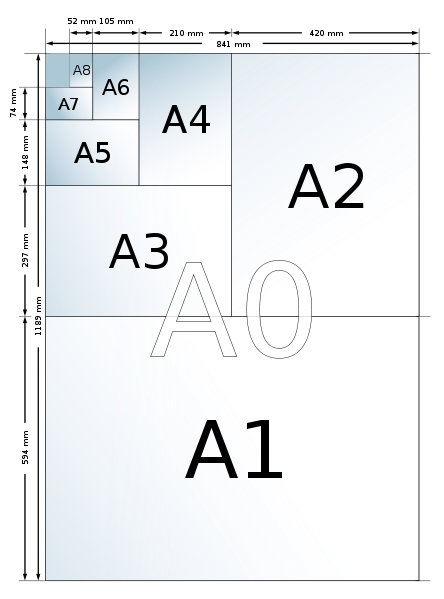
\includegraphics[width=0.5\linewidth]{./graphics/A-sizes.png}
  \caption{When a sheet whose proportions are $1$:$\surd{2}$ is folded in half, the result is a sheet half as large but with \emph{the same proportions}. Standard paper sizes on this principle have been in use in Germany since the early 1920s. The basis of this system is the A0 sheet, which has an are of 1 m$^2$. Yes because it is \textit{reciprocal with nothing but itself}, the ISO page in isolation is the least musical of all the major page shapes. It needs a textblock of another shape or contrast.}
   \label{fig:marginfig1}
\end{figure}

The advantages of basing a paper size upon an aspect ratio of $\surd{2}$ were already noted in 1786 by the German scientist Georg Christoph Lichtenberg, in a letter to Johann Beckmann[2]. The formats that became |A2|, |A3|, |B3|, |B4| and |B5| were developed in France, and published in 1798 during the French Revolution, but were subsequently forgotten. \cite{letimbre2136}

Early in the twentieth century, Dr Walter Porstmann turned Lichtenberg's idea into a proper system of different paper sizes. Porstmann's system was introduced as a DIN standard (DIN 476) in Germany in 1922, replacing a vast variety of other paper formats. Even today the paper sizes are called "DIN Ax" in everyday use in Germany.

The main advantage of this system is its scaling: if a sheet with an aspect ratio of $\surd{2}$ is divided into two equal halves parallel to its shortest sides, then the halves will again have an aspect ratio of $\surd{2}$. Folded brochures of any size can be made by using sheets of the next larger size, e.g. |A4| sheets are folded to make |A5| brochures. The system allows scaling without compromising the aspect ratio from one size to another – as provided by office photocopiers, e.g. enlarging |A4| to |A3| or reducing |A3| to |A4|. Similarly, two sheets of |A4| can be scaled down and fit exactly 1 sheet without any cutoff or margins.

%\cxset{try grid=false}
%\thispagestyle{grid}


The weight of each sheet is also easy to calculate given the basis weight in grams per square metre (g/m² or `'gsm"). Since an |A0| sheet has an area of 1m² , its weight in grams is the same as its basis weight in g/m². A standard |A4| sheet made from 80 g/m² paper weighs 5g, as it is one 16th (four halvings) of an A0 page. Thus the weight, and the associated postage rate, can be easily calculated by counting the number of sheets used.

Unlike the |A4| standard paper, the origin of the dimensions of letter size paper are lost in tradition. The American Forest and Paper Association argues that the dimension originates from the days of manual paper making, and that the 11-inch length of the page is about a quarter of ``the average maximum stretch of an experienced vatman's arms".[1] However, this does not explain the width or aspect ratio. What is known is that Ronald Reagan made this the paper size for U.S. federal forms; previously, the smaller "official" size (8 in × 10½ in or 203.2 mm × 266.7 mm) was used.[1] Letter or US Letter is the most common paper size for office use in the United States and Canada. It is 8$\frac{1}{2}$ by 11 inches (exactly 215.9 mm × 279.4 mm).

\section{The Typearea}

According to \cite{bringhurst2005}, in typography margins must do three things. They must lock the
textblock to the page and lock the facing pages to each other through the force of their proportions. Second, they must frame the textblock in a manner that suits its design. Third, they must protect the textblock, leaving it easy for the reader to see and convenient to handle. 

In most well designed books fifty per cent of the character and integrity of a printed page lies in its letterforms. Much of the other fifty per cent resides in its margins.


\subsection{Readability}

Another aspect that determines the text area, is the readability of the text. Here you need to take into account the readers of your book. For children and older persons a larger type and shorter lines are preferred.

\begin{macro}{\alphabetlength}
The macro |\alphabetlength| prints the length of the alphabet. The length of the alphabet in this text is \alphabetlength. If this is a good choice is debatable, but after all this is just a long document, with many chapters and my aim was to produce a reference and a test document. The macro is defined in the |xlayouts|  package, which is loaded automatically by the |phd| package or class. 
\end{macro}

Traditionally  a line that is approximately 1.4 times the alphabet length is considered good practice. The length of one line of text in this document is \the\textwidth giving a ratio of \alphabetsperline.

\DescribeMacro{\printreadability} prints a small table with some readability figures. If LuaTeX is used, this table is slightly longer and prints some other statistics as well. 

\begin{figure}[htbp]
\drawtriallayout
\bigskip

\printreadability
\captionof{figure}{Page layout diagram and readability statistics (using the \pkgname{xlayouts} package).}
\end{figure}

The macros described above are loaded by the |xlayouts| package, which forms part of the |phd| budle. There are macros for drawing trial layouts 


\section{Examples}
Folowing the nomenclature introduced b Bringhurst in analyzing the examples on the following pages, 
these symbols are used:

%% Align at the = sign 
\begin{table}[htbp]
\begin{tabular}{l l @{ = } p{6cm}}
\textit{Proportions:}      &P  &  page proportion $h/w$\\
~                      &T &  textblock proportion: $d/m$\\
\textit{Page size:}         &w &  width of page (trim-size)\\
~                      &h  & height of page (trim-size)\\
\textit{Textblock:}           &m & measure (width of primary textblock)\\
~                      &d  & depth of primary textblock (excluding running heads, folios etc)\\                      
~                      &$\lambda$ & line height (type size plus added lead)\\
~                      &$n$ & secondary measure (width of secondary column)\\
~                      &$c$  & column width, where there are even multiple columns\\
\textit{Margins}  &$s$  & spine margin (back margin)\\
~                      &$t$   & top margin (header margin)\\
                        &$e$  & fore-edge (front margin)\\
                        &$f$   & foot margin\\
                        &$g$  & internal gutter (on a multiple-column page)\\
\end{tabular}
\caption{Symbols used to demonstrate various ratios in books}
\end{table}
\medskip

\begin{figure}
  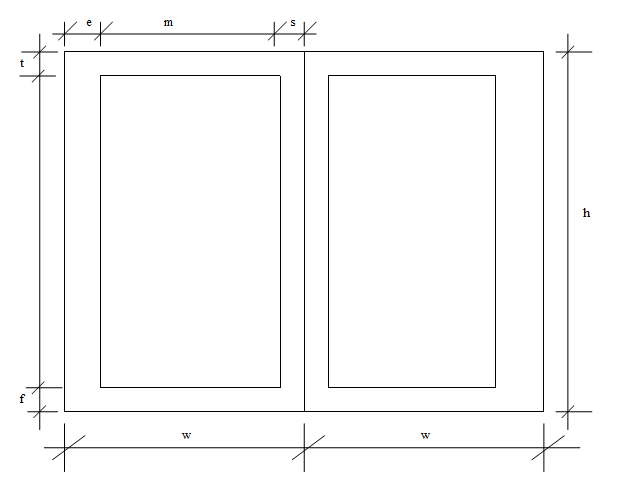
\includegraphics[width=\linewidth]{./graphics/page.png}
  \caption{Page nomenclature}
   \label{fig:marginfig1}
\end{figure}

More variables are necessary to specify all the variables handled by a \latex\
page. For the time being the examples refer to dimensions from historical works
in typography and should sufffice.

\subsection{Hypneroto}

\begin{figure}[htbp]
\centering
  \includegraphics[width=\linewidth]{./graphics/hypneroto.jpg}
\caption{The work is lauded for the originality of its
design. Several sequential double page
illustrations add a visual dimension to the
progression of the narrative, and act like an
early form of the strip cartoon. There is an
obsession with movement throughout which is driven
on by the illustrations, resulting in the
impression of bodies moving from one page to the
next. Other typographical innovations include
playing with the traditional layout of the text;
in the opening shown here, for example, the pages
are shaped in the form of goblets. The dimensions
of the text are: $P=1.5[2:3]$; T=1.7 (tall pentagon);
Margins: s=t=w/9; e=2 s. The text is a fantasy
novel, Francesco Colonna's Hypnerotomachia
Poliphili, set in a roman font cut by Francesco
Griffo. (Aldus Manutius, Venice, 1499). Original
size: $20.5\times31$\thinspace cm.}
\label{fig:hypneroto}
\end{figure}


%  \label{fig:layout}



The book was printed by Aldus Manutius in Venice in December 1499. The book is anonymous, but an acrostic formed by the first, elaborately decorated letter in each chapter in the original Italian reads \textsc{\small POLIAM FRATER FRANCISCVS COLVMNA PERAMAVIT}, \enquote{Brother Francesco Colonna has dearly loved Polia.} However, the book has also been attributed to Leon Battista Alberti by several scholars, and earlier, to Lorenzo de Medici. The latest contribution in this respect was the attribution to Aldus Manutius, and arguably, a Francesco Colonna, a wealthy Roman Governor. The author of the illustrations is even less certain, but contemporary opinion gives the work to Benedetto Bordone.

\section{Contemporary book layouts}

All these sound mystical with religious undertones, but we need to remember that early printers made their livelihoods from printing mostly religious books.

From the mystics to the modern, let us study Figure~\ref{fig:nudes}

\begin{figure}[htbp]
\centering

\fbox{\includegraphics[width=\linewidth]{nudes.jpg}}

\caption{In this layout, the placement of various size images on the right pages, makes the margins disappear to the eye. As the whole book, is made of similar pages\ldots }
\end{figure}

Modern designers are more cryptic. One book that I found more useful is Ambrose/Harris \textit{Layout}. The book brings together examples of layout, both contemporary  and historic, from aroudnd the world. It contains examples from leading graphic designers to provide a sample of rich and diverse possibilities for the creative use of layout.

As it will become apparent from what follows, although at first look it appears that all design principles have disappeared into post modern designs, all design is undertaken with reference to a certain set of principles, either by consciously
choosing to follow or by deliberately ignoring or subverting them. The collective body of principles represents different approaches to design and layout construction.

The principles in this section have been used
through the ages to produce designs that are
pleasing to the eye and that organise information
clearly and efficiently, two of the challenges facing
every graphic designer. These principles affect
decisions made at the heart of the design process,
as they provide the basis of how space is divided.

\section{A design must capture the spirit of the times.}

The word \emph{zeitgeist} originates from the German zeit (time) and geist (spirit),
and so literally means spirit of the age. In graphic design, each decade can
be defined by several predominant zeitgeists that somehow seem to capture
their essence. Today, in graphic design, we can see a zeitgeist for the use of
sophisticated computer graphics giving a very close approximation to reality
in addition to another, which is a backlash to this, in the form of rough-and-ready
hand-drawn designs.

\section{Objects on a Page}

How an object is placed on a page has a dramatic
impact on how it is received and interpreted by
the viewer, and the message that it delivers. We
have looked at how grids can be used to guide
element placement on a page, but maintaining a
sense of order is not the only consideration when
laying out a design.

Object placement helps form the narrative of
a design and is constructed from an understanding
of how we read a page. The narrative of a design
can be created and altered by a wide range of
placement and intervention strategies, such as
how white space is used, the balance and relative
weight given to other objects, the juxtaposition or
contrast of objects and so on.

This chapter will outline some of the
fundamental approaches to object placement.

\section{White Space}

White space is not necessarily white, as it refers to any space in the design
without text or graphic elements. Designers naturally insert white space into
their designs to help the composition and make the information the design
contains easier to access, such as leaving margins at the sides of the page that
create space around text blocks. Swiss typographer Jan Tschichold called white
space ‘the lungs of a good design’. Without white space, with every part of the
design area filled, there is a danger that a design would look cramped and
difficult to understand.

White space can instil different perceptions in a viewer depending on how it is
used and the content it is associated with. White space may give the impression
of luxury and extravagance for a full-page photograph. However, it may also give
the impression that there are gaps in a layout that is rather full, or worse, that
there is insufficient content to fill a page. Newspapers try to establish a rational
balance between giving space to page elements to meet the conflicting demands
of the need for typographical sensitivity and readability, while filling a page with
news so that the reader feels they are getting value for money. Habitually readers
expect a newspaper to be ‘full’, which means it is harder to achieve typographic
balance. In contrast, where filling space is of less concern, such as the example
below, white space becomes a more overt part of the design.



\section{Grids}

\subsection{The Baseline Grid}

The baseline grid is the (invisble) graphic foundation upon which a design is constructed and provides a visual guide for positioning and ligning page elements with an accuracy that is difficult to achieve by eye alone. Knuth's TeX focuses almost primarily on getting this one right.

\section{Pace}

It came to me as a big surprise that a books layout must have \textit{pace}. This essentially is the alternation of pages, between say images and text.

\begin{figure}[htbp]
\parindent=0pt
\includegraphics[width=\textwidth]{pace}

\end{figure}

Thumbnails are smaller versions of the spreads of a publication presented on a
page that allow a designer to gauge its pace and balance at the macro level
without focusing on details. Thumbnails allow a designer to look at the
narrative of the publication and tune it as a whole, rather than on a spread-byspread
basis.

Pictured are thumbnails for Miss X, a book for underwear retailer Agent
Provocateur art directed by Mike Figgis and published by Anova, with design by
Gavin Ambrose. The absence of folios and minimal text mean the image flow
takes prominence.

The images can let us set a method for defining such spreads. 


\chapter{Temporarily changing the text width}

\index{pagewidth>change temporarily}


Margins in a page can be changed temporarily by adjusting, the lengths of \cmd{\leftskip} and \cmd{\rightskip}. The |memoir| class provides an environment |adjustwidth| see page 422 (based on This code is based on the \pkgname{chngpage} package.) for doing so and the \class{tufte-book} class provides an environment \textit{fullwidth}. The following code is an adaptation of that found in the \class{memoir} class.


\begin{teXX}
\begin{adjustmargins}{left}{right} 
\end{teXX}


adds the given lengths to the left and
right hand margins. A positive value will shorten the text and a negative value
will widen it. The starred version of the environment will cause the margin changes to switch between odd and even pages. 



\eject
\newgeometry{left=10mm,right=10mm,bottom=1.5cm,top=1cm}

\section*{The \texttt{adjustmargins} environment}
\lorem

\vfill\vfill
\begin{multicols}{2}
\lorem
\end{multicols}

\begin{adjustmargins}{0cm}{0in}
{\leftskip1em\rule{13cm}{.4pt}\par}

\centering



\parbox{\textwidth}{{\leftskip1em\rightskip1em There are no engineers in the hottest parts of hell, because the existence of a 'hottest part' implies a temperature difference, and any marginally competent engineer would immediately use this to run a heat engine and make some other part of hell comfortably cool.  This is obviously impossible.\par}
}
\par
\medskip
\par
\noindent\includegraphics[width=0.9\textwidth]{./graphics/lilian.jpg}\par


\end{adjustmargins}

\clearpage

\restoregeometry


\lipsum[1]


\begin{adjustmargins}{-0.4\textwidth}{0.1\textwidth}
\fboxsep2pt%
\fbox{\includegraphics[width=1.2\textwidth]{./graphics/leoncroll.jpg}}
\end{adjustmargins}

\lipsum[2]

\begin{teX}
\begingroup
\makeatletter
 \catcode`\Q=3
 \long\gdef\@ifmtarg#1{\@xifmtarg#1QQ\@secondoftwo\@firstoftwo\@nil}
 \long\gdef\@xifmtarg#1#2Q#3#4#5\@nil{#4}
 \long\gdef\@ifnotmtarg#1{\@xifmtarg#1QQ\@firstofone\@gobble\@nil}
 \endgroup


\newenvironment{adjustmargins}[2]{%
  \begin{list}{}{%
    \topsep\z@%
    \listparindent\parindent%
    \parsep\parskip%
   \@ifmtarg{#1}{\setlength{\leftmargin}{\z@}}%
   {\setlength{\leftmargin}{#1}}%
   \@ifmtarg{#2}{\setlength{\rightmargin}{\z@}}%
   {\setlength{\rightmargin}{#2}}%
}
\item[]}{\end{list}}
\makeatother
\end{teX}

 
\section{Setting Dimensions in \latex}

To set dimensions for page layout in \latex is not straightforward. You need to adjust several \latex
native dimensions to place a text area where you want. If you want to center the text area in the paper
you use, for example, you have to specify native dimensions as follows:

\begin{verbatim}
\usepackage{calc}
\setlength\textwidth{7in}
\setlength\textheight{10in}
\setlength\oddsidemargin{(\paperwidth-\textwidth)/2 - 1in}
\setlength\topmargin{(\paperheight-\textheight
-\headheight-\headsep-\footskip)/2 - 1in}.
\end{verbatim}

Without package |calc|, the above example would need more tedious settings. To adjust all parameters from scratch one should have a good understanding, of \latexe's definitions of all parameters. The companion package |xlayouts| can be used to display these parameters on an actual printed page. All settings are parameterized and I find the use of colours assists in viewing the rulers better.


\subsection{The Geometry package}

The package \pkg{geometry} \cite{geometry} provides
an easy way to set page layout parameters. In this case, what you have to do is just load the package and set
the page geometry using keys.

\begin{teX}
\usepackage[text={7in,10in},centering]{geometry}.
\end{teX}

Besides centering problem, setting margins from each edge of the paper is also troublesome. But geometry
also make it easy. If you want to set each margin to 1.5in, you can type

\begin{comment}
\label{sec:geometry}

\def\OpenB{{\ttfamily\char`\{}}
 \def\Comma{{\ttfamily\char`,}}
 \def\CloseB{{\ttfamily\char`\}}}
 \def\Gm{\textsf{geometry}}
\newcommand\gpart[1]{\textsf{\textsl{\color[rgb]{.0,.45,.7}#1}}}%

\newcommand\glen[1]{\textsf{#1}}

\bgroup
\makeatletter
 \begin{figure}
  \small
  \unitlength=.65pt
  \begin{picture}(450,250)(0,-10)
  \put(20,0){\framebox(170,230){}}
  \put(20,235){\makebox(170,230)[br]{\gpart{paper}}}
  \begingroup\thicklines
  \put(40,30){\framebox(120,170){}}
  \put(40,30){\makebox(120,165)[tr]{\gpart{total body}~}}
  \put(45,30){\makebox(0,170)[l]{|height|}}
  \put(40,35){\makebox(120,0)[bc]{|width|}}
  \put(50,-20){\makebox(120,0)[bc]{|paperwidth|}}
  \put(10,45){\makebox(0,170)[r]{|paperheight|}}
  \put(90,200){\makebox(0,30)[lc]{|top|}}
  \put(90,0){\makebox(0,30)[lc]{|bottom|}}
  \put(10,70){\makebox(0,0)[r]{|left|}}
  \put(10,55){\makebox(0,0)[r]{(|inner|)}}
  \put(200,70){\makebox(0,0)[l]{|right|}}
  \put(200,55){\makebox(0,0)[l]{(|outer|)}}
  \put(80,230){\vector(0,-1){30}}\put(80,30){\vector(0,-1){30}}
  \put(80,200){\vector(0,1){30}}\put(80,0){\vector(0,1){30}}
  \put(20,70){\vector(1,0){20}}\put(40,70){\vector(-1,0){20}}
  \put(160,70){\vector(1,0){30}}\put(190,70){\vector(-1,0){30}}
  \multiput(160,30)(5,0){24}{\line(1,0){2}}
  \multiput(160,200)(5,0){24}{\line(1,0){2}}
  \begingroup\thicklines
  \put(280,30){\framebox(120,170){}}\endgroup
  \put(283,133){\makebox(0,12)[l]{|textheight|}}
  \put(295,130){\vector(0,-1){100}}\put(295,150){\vector(0,1){50}}
  \multiput(280,220)(5,0){24}{\line(1,0){3}}
  \put(280,208){\makebox(120,20)[bc]{\gpart{head}}}
  \multiput(280,207)(5,0){24}{\line(1,0){3}}
  \put(420,225){\makebox(0,0)[l]{|headheight|}}
  \put(418,225){\line(-2,-1){20}}
  \put(420,213){\makebox(0,0)[l]{|headsep|}}
  \put(418,213){\line(-2,-1){20}}
  \put(420,12){\makebox(0,0)[l]{|footskip|}}
  \put(418,12){\line(-2,1){20}}
  \put(280,40){\makebox(120,140)[c]{\gpart{body}}}
  \put(305,45){\vector(-1,0){25}}\put(375,45){\vector(1,0){25}}
  \put(80,230){\vector(0,-1){30}}\put(80,30){\vector(0,-1){30}}
  \put(280,48){\makebox(120,0)[c]{|textwidth|}}
  \put(280,15){\makebox(120,10)[c]{\gpart{foot}}}
  \multiput(280,14)(5,0){24}{\line(1,0){2}}
  \put(410,30){\dashbox{3}(30,170){}}
  \put(415,30){\makebox(30,170)[l]{\gpart{marginal note}}}
  \put(425,45){\vector(-1,0){15}}\put(425,45){\vector(1,0){15}}
  \put(450,70){\makebox(0,0)[l]{|marginparsep|}}
  \put(448,70){\line(-3,-1){43}}
  \put(450,45){\makebox(0,0)[l]{|marginparwidth|}}
  \end{picture}
\caption{Dimension names used in the geometry package. width $=$ textwidth and height $=$ textheight by default. left, right, top and bottom are margins. If margins on verso pages are swapped by twoside option, margins specified by left and right options are used for the inside and outside margins respectively. inner and outer are aliases of left and right
respectively.}
\label{fig:geometrylayout}
\end{figure}
\makeatother
\egroup
\end{comment}

 The \pkg{geometry} package provides a flexible and easy interface to page dimensions.
 You can change the page layout with intuitive parameters. For instance,
 if you want to set a margin to 2cm from each edge of the paper,
 you can type just |\usepackage[margin=2cm]{geometry}|. 
 The page layout can be changed in the middle of the document
 with \cs{newgeometry} command.  The \ref{fig:geometrylayout}, reproduced from the package documentation, illustrates the variety of parameters that can be set using the package.


\section{Footnotes}
The history of footnotes is as long and complicated as the history of scholarship and commentary. Hebrew scholars more than two thousand years ago used systems of glossing and annotation to work on religious texts. 

Scribes in the Christian tradition in the medieval period made use of annotations in their manuscript copying practices: surrounding the original text with glosses in small letters. After the advent of printing, similar kinds of marginal annotation appeared in printed texts of the late fifteenth century. 

Humanist scholars producing printed editions of classical learning in the sixteenth century also made use of the resources of typography to display both the surviving classical text and their commentary on the same page. References to classical sources - and to modern printed editions - became more systematic, as did the expectation that such references would be consistent with scholarly practices. Scholars increasingly marked their professionalism by using complex citational conventions, which by the seventeenth century were so well established as to be the subject of parody and satire. Scriblerian satire of the early eighteenth century, whose purpose was to mock the pedantry and folly of the works of the learned, frequently included extensive parodies of footnotes and the scholarly contests they encoded. Nonetheless, during the eighteenth century, to appear authoritative and learned an author had to adopt the scholarly machinery of the reference citation.

The footnote was born out of a desire to rationalise the relation between text and citation. 

Robert Connors argues that marginal notations fell out of favour for two practical reasons: they left too much blank paper at the side of the text; and they were difficult for typographers to set. The same notes placed at the bottom of the page were more efficient, both in paper and time[1]. 

Anthony Grafton's The Footnote: A Curious History suggests the modern footnote, inaugurated by Pierre Bayle's Dictionaire Critique et Historique in 1697, signalled an epistemic revolution in historical scholarship, indicating the end of credulous scholasticism and the emergence of analytical historical methodologies. Both scholars note the considerable impact of historians such as David Hume and Edward Gibbon on the stylistic development of the discursive and citational footnote as a location for the display of gentlemanly ease as much as scholarly acumen. In the nineteenth century, German scholars such as Leopold von Ranke and Alexander von Humboldt established a systematic basis for the footnote citation, creating a methodical methodological approach that all competing scholars had to obey. In this way, the idea of the footnote was established, yet no there was no general agreement on the form these footnotes should adopt. A systematic approach to the form of the footnote was needed.

In this section we will discuss how lines and paragraphs are turned into pages and how elements of pages such as footnotes, headers etc are inserted. As with the other chapters we will mix TeX basic commands with the more convenient \LaTeXe\ commnads. We will also look at some of the packages and classes that are availble to assist us with page layouts. 


Besides illustrations that are inserted at the top of a page, plain TEX will also
insert footnotes at the bottom of a page. The ootnote macro is provided
for use within paragraphs;  for example, the footnote in the present sentence was typed
in the following way:


There are two parameters to a footnote[ first comes the reference mark, which will
appear both in the paragraph** and in the footnote itself, and then comes the text of
the footnote.45 The latter text may be several paragraphs long, and it may contain
\footnote{Sidenote: ``Where God meant footnotes to go.'' ---Tufte}

\marginpar{

The history of footnotes is as long and complicated as the history of scholarship and commentary. Hebrew scholars more than two thousand years ago used systems of glossing and annotation to work on religious texts. Scribes in the Christian tradition in the medieval period made use of annotations in their manuscript copying practices: surrounding the original text with glosses in small letters. After the advent of printing, similar kinds of marginal annotation appeared in printed texts of the late fifteenth century. Humanist scholars producing printed editions of classical learning in the sixteenth century also made use of the resources of typography to display both the surviving classical text and their commentary on the same page. References to classical sources - and to modern printed editions - became more systematic, as did the expectation that such references would be consistent with scholarly practices. Scholars increasingly marked their professionalism by using complex citational conventions, which by the seventeenth century were so well established as to be the subject of parody and satire. Scriblerian satire of the early eighteenth century, whose purpose was to mock the pedantry and folly of the works of the learned, frequently included extensive parodies of footnotes and the scholarly contests they encoded. Nonetheless, during the eighteenth century, to appear authoritative and learned an author had to adopt the scholarly machinery of the reference citation.

The footnote was born out of a desire to rationalise the relation between text and citation. Robert Connors argues that marginal notations fell out of favour for two practical reasons: they left too much blank paper at the side of the text; and they were difficult for typographers to set. The same notes placed at the bottom of the page were more efficient, both in paper and time[1]. Anthony Grafton's The Footnote: A Curious History suggests the modern footnote, inaugurated by Pierre Bayle's Dictionaire Critique et Historique in 1697, signalled an epistemic revolution in historical scholarship, indicating the end of credulous scholasticism and the emergence of analytical historical methodologies. Both scholars note the considerable impact of historians such as David Hume and Edward Gibbon on the stylistic development of the discursive and citational footnote as a location for the display of gentlemanly ease as much as scholarly acumen. In the nineteenth century, German scholars such as Leopold von Ranke and Alexander von Humboldt established a systematic basis for the footnote citation, creating a methodical methodological approach that all competing scholars had to obey. In this way, the idea of the footnote was established, yet no there was no general agreement on the form these footnotes should adopt. A systematic approach to the form of the footnote was needed.}

Further reading:

Connors, Robert J., 'The Rhetoric of Citation Systems, Part I: The Development of Annotation Structures from the Renaissance to 1900', Rhetoric Review, 17 (1998), 6-48.

Connors, Robert J., 'The Rhetoric of Citation Systems, Part II: Competing Epistemic Values in Citation', Rhetoric Review, 17 (1999), 219-245.

Grafton, Anthony, The Footnote: A Curious History (London: Faber and Faber, 1997)

Grafton, Anthony, 'The Footnote from De Thou to Ranke', History and Theory, 33 (1994), 53-76

Zerby, Chuck, The Devil's Details: A History of Footnotes (Lancaster: Gazelle, 2002)

[1] Robert J. Connors, The Rhetoric of Citation Systems, Part I: The Development of Annotation Structures from the Renaissance to 1900, Rhetoric Review, 17 (1998), 6-48 (p. 30).
 
%\makeatletter

\cxset{geometry textwidth/.store in=\textwidth@cx,
          geometry textheight/.store in=\textheight@cx,
          geometry tufte/.code={
             \newgeometry{a4paper,left=24.8mm,top=27.4mm,headsep=2\baselineskip,%
             textwidth=107mm,marginparsep=8.2mm,marginparwidth=49.4mm,%
             textheight=\textheight@cx\baselineskip,
             headheight=\baselineskip}
            \@twosidefalse \@mparswitchfalse 
    }
}


\def\pregeometry{\geometry{%
     left=74.8mm,
     top=27.4mm,
     headsep=2\baselineskip,%
     marginparsep=8.2mm,
     marginparwidth=49.4mm,
     textheight=\textheight@cx\baselineskip,%
     headheight=\baselineskip}%
     \@twosidefalse \@mparswitchfalse %
     \reversemarginpar}
     
     
\def\postgeometry{  \newgeometry{%
     left=74.8mm,
     top=27.4mm,
     headsep=2\baselineskip,%
     marginparsep=8.2mm,
     marginparwidth=49.4mm,
     textheight=\textheight@cx\baselineskip,%
     headheight=\baselineskip}%
     \@twosidefalse \@mparswitchfalse %
     \reversemarginpar}
     
\cxset{geometry oxford/.code=
\if@phdpreamble
    \expandafter\pregeometry
   \else
    \expandafter\postgeometry
   \fi
 }
   
  


\cxset{geometry textheight=49,
          geometry oxford,
           }
\cxset{marginpar push/.store in=\marginparpush@cx,
          marginpar font/.store in=\marginparfont@cx,
          marginpar justification/.is choice,
          marginpar justification/justifying/.code=\gdef\marginparjustification@cx{\justifying},
          marginpar justification/raggedright/.code=\gdef\marginparjustification@cx{\raggedright},
          marginpar justification/RaggedRight/.code=\gdef\marginparjustification@cx{\RaggedRight},
          marginpar justification/RaggedLeft/.code=\gdef\marginparjustification@cx{\RaggedLeft},
 }
\cxset{marginpar push=10pt,
          marginpar font=\normalfont\footnotesize\sffamily,
          marginpar justification=RaggedLeft}



%This is a sidenote without the footnote mark
\newcommand\marginnote[2][0pt]{%
  \marginpar{\hbox{}\vspace*{#1}\marginparfont@cx\marginparjustification@cx\vspace*{-1\baselineskip}\noindent #2}%
             
}


\def\asidecaption{\parbox{\marginparwidth}{{\bfseries Image \thefigure}\par\lorem}%
  \addtocontents{lof}{This is image 8}
}

\def\ps@caption{%
     \let\@oddfoot\@empty\let\@evenfoot\@empty%
     \edef\leftx{-\marginparwidth-\marginparsep}
    \def\@evenhead{%
           \begin{picture}(0,0)%
           \put(-\marginparwidth-\marginparsep,-\headheight-\topsep-5pt){ \line(1, 0){\marginparwidth}}%
           \put(-\marginparwidth-\marginparsep,-\headheight-\headsep){ \line(1, 0){\marginparwidth}}%
            \put(\leftx,-90){\asidecaption\par}%
            \stepcounter{figure}%
           \put(\leftx,-370){\asidecaption}%
        \end{picture}%
      }%
    \let\@oddhead\@evenhead%
    \let\@mkboth\@gobbletwo%
    \let\chaptermark\@gobble%
    \let\sectionmark\@gobble%
 }

\def\ps@bigpicture{%
    \setlength\headheight{19cm}%
    \let\@oddfoot\@empty\let\@evenfoot\@empty%
    \def\@evenhead{%
         \begin{picture}(0,0)%
          \put(-149,0){\includegraphics[width=\dimexpr(\textwidth+150pt)]{stuartpearson}}%
         \end{picture}%
      }%
    \let\@oddhead\@evenhead%
    \let\@mkboth\@gobbletwo%
    \let\chaptermark\@gobble%
    \let\sectionmark\@gobble%
 }


\def\doubletakeimage{%
  \renewcommand{\topfraction}{.95}%
  \begin{figure}[t]
      \includegraphics[width=\textwidth]{matron}%
       \thispagestyle{caption}
  \end{figure}

  \begin{figure}[tp]
   \hspace*{-\marginparwidth}\includegraphics[height=0.9\textheight]{stuartpearson}
 \end{figure}
}



\chapter{Geometry and Page Dimensions}

Many modern books have pages with large margins, where either images or notes are added. The style we will
examine has mostly the captions of images. The advantage of such layouts is that firstly it improves the readability of the text by having shorter lines and secondly the images have reasonable dimensions. They also look very
good.

The textual treatment can easily be handled by \latexe so we will not be spending too much time discussing it, as 
we will focus our attention on the treatment of images and their captions.

The first thing we need to do is to specify the geometry of the page. Unlike Tufte’s books the Oxford University Press as well as the Cambridge University Press have all the margin material at the left. The \pkgname{phd} provides a style for such geometry named \textbf{oxford}

\begin{scriptexample}{}{}
\begin{verbatim}
\cxset{geometry=oxford}
\end{verbatim}
\end{scriptexample}

The interesting aspect of this style is the asynchronous floating of the margin captions as compared with
the images. 

\latexe’s   cs{marginpar} has not been designed with such problem in mind and is notoriously difficult
to get right especially if there are a lot of margninal material. The method I am proposing for here
is to use some of the abilities of pdfTeX engine to leverage the routines by using absolute positioning
thus in a way, we will build our own output routine rather than using the primitive cs{output} to process
the placement of the algorithm for images and their captions. 

Although the style is essentially what is termed a \texttt{oneside} style in real terms the captions (depending on the image size)  need to know if they are to be placed next to the image or at the previous page or at the next page margin. In practical terms the margin becomes another page. The typographical algorithm is described in the next section and the placement of the margin is a function of the image height and the set of page parameters $f: (i_h, p_m)$. 
For example if a page is a chapter opening page and is preceded  by a full page image then the caption is almost universally palaced at the bottom of the the chapter opening margin.

If we are to try and do all the manipulation ourselves rather than leaving it to standard \latexe routines, we will
need some helper macros and also we need to decide on the interaface we want to offer the user. 

\doubletakeimage

\section{Handling the image captions}

At first look the images should not present any difficulties and could be handled by normal
floating \latexe objects. On closer examination the larger images will need special treatment. In Fig~\ref{unequal}
the figure is shown as fullwidth, with the image caption placed in the margin of the \emph{previous} page. One of the major limitations of the \tex typesetting engine is that once a page is constructed the information on that page is lost. Before we attempt to program the palcements, let us define typographical rules for such image placements.

\begin{enumerate}
\item Measure the image width. If the image is $\le l_t$ then the image can be placed either at the top
         or bottom of the page and the side caption at the left of the image.
\item Measure the image height ($h_i$) and the height of the image caption ($h_{i,c}$). If the sum of the two exceeds the limit $l_m$ then signal that the image caption must be placed at the margin of the left page. If it does not then place it at the same page on top of the image.

\item Write the page object-1 to the auxiliary file.

\item When reading the auxiliary place the caption at the margin of the previous page. The placement will
depend on other marginal material, but preferably balance it by placing it at the bottom. 
\end{enumerate}
  
The central idea would be to write to the auxiliary file for every page, some information that we want to preserve
then we can by-pass to a large extend the output routine and tex engine limitations.

The information we need to be stored as an object of the form.

\begin{verbatim}
pagenumber = object(marginmaterial, placement preferences)
t = {pagenumber,
       image,
       caption,
       caption placement rules
       caption placement manual adjustments}
\end{verbatim}
 
\begin{figure}[tbp]
\fbox{\includegraphics[width=\textwidth]{2-unequal-02}}
\caption{Page construction with the caption of the right page image, being placed on the margin of the page at the left. There is no standard way to automate such captions and images with \latexe, but with manual
intervention it is possible.}
\label{unequal}
\end{figure}

Another issue we need to handle is that images that are full width and height need to be treated differently. If they are on an even page then the caption needs to be moved forward to the next right page and placed either at the top or bottom, depending if the page has other images, if it is a heading opening page and the like.

The central idea to the algorithm is that all pages will have a page object defined and stored in the auxiliary
file. 

To achieve this we will try and define the objects using Lua rather than normal \tex routines although it could be as easy to do it with \tex commands. Writing to the auxiliary file should take place when we are in the output routine so that we can pick up the page number. This asynchronous or rather stateless output routine can be bypassed this way.\marginnote{See also similar routines that were developed as an extension to the Tufte-class.}

\begin{figure}[tbp]
\centering

\fbox{\includegraphics[width=\textwidth]{elizabeth}}

\caption{Page construction with the captioe  of the right page image, being placed on the margin of the page at the left. There is no standard way to automate such captions and images with \latexe, but with manual
intervention it is possible.}

\label{elizabeth}
\end{figure}

\begin{enumerate}
\item If full height image. If at the left page caption need to be placed at the right page.
\item If the right page has an image the caption of the left page needs to be placed first.
         For an example of this rule see Figure~\ref{elizabeth}.
\end{enumerate}

\section{Full width two images}

\begin{figure}[tbp]
\fbox{\includegraphics[width=\textwidth]{bazille}}
\caption{Page construction with the caption  of the right page image, being placed on the margin of the page at the left. There is no standard way to automate such captions and images with \latexe, but with manual
intervention it is possible.}
\label{elizabeth}
\end{figure}

Another interesting observation is what to do when we have to fullwidth images on the page. Again in ths case the image captions are placed on the next page. Here the captions are placed at preferred locations. The first caption
is set flush with the top margin and the second one is placed at the same height as the top of the image. What this means is that when the images are typeset we will  need to also store the position of the object at the page. This can also be observed on larger images see Figure~\ref{laura}

\begin{figure}[tbp]
\fbox{\includegraphics[width=\textwidth]{laura}}
\caption{Page construction with the captioe  of the right page image, being placed on the margin of the page at the left. There is no standard way to automate such captions and images with \latexe, but with manual
intervention it is possible.}
\label{elizabeth}
\makeatletter
%\write\@auxout{\protect\def\hello{hello \thepage}}


\end{figure}

\restoregeometry
A RESET EVERYTHING AT END OF CHAPTER


\addtocounter{chapter}{-2}
\@toctrue\@specialtrue

\makeatother     
%       
%\def\storyi{The best graphics package ever developed is the TikZ package. 
Its parent package is PGF which is short of a miracle that has been programmed
using \tex, a more than thirty years old program. This has taken over almost all other
packages and is very popular with newcomers to \latex. It is frustrating at first, but once 
you over the basic ideas and concepts it opens infinite possibilities for typesetting
great articles and books.}



\cxset{chapter format=stewart,
       texti=\storyi,
       textii=\storyi}

\newcommand\seepgfmanual[1]{%
    \textit{see} the PGFmanual page #1}%
    
%\cxset{chapter format = traditional}    
\chapter{TikZ}

\section{The \protect\texttt{TikZ} package}
\pkg{TikZ}, a high-level interface to \pkg{PGF}, is a language-based tool for specifying graphics.
It uses familiar graphics-related concepts, such as point, line, and circle and
has a concise and natural syntax. It meshes well with pdfLATEX in the sense that
no additional processing steps are needed. Another positive aspect of \pkg{TikZ} is
its ability to blend \tex fonts, symbols, and mathematics within the generated
graphics
.
\begin{center}
\begin{tikzpicture}

\draw (0,0) ellipse (5 and 1.8);

\filldraw [black]  (-3,-0.5) circle (1pt);

\filldraw [black] (0.5,-0.5) circle (1pt);
\filldraw [black] (1.5,-0.5) circle (1pt);
\filldraw [red] (1.0,0.5) circle (1pt);
\filldraw [green] (2.0,0.5) circle (1pt);


\draw [->>] (0.5,-0.5) .. controls (0.5,-0.2) and (0.7,0.3) .. (0.9,0.45);
\draw [->>] (1.5,-0.5) .. controls (1.5,-0.2) and (1.7,0.3) .. (1.9,0.45);

\draw (-3.1,-0.5) node[anchor=east]  {$1_G$};

\draw (0.5,-0.5) node[anchor=north] {$g$};
\draw (1.5,-0.5) node[anchor=north] {$gs$};
\draw (1.0,0.5) node[anchor=south] {$gt$};
\draw (2.0,0.5) node[anchor=south] {$gst$};
\draw (0.5,-0.5)-- (1.5,-0.5);


\end{tikzpicture}
\end{center}

All the TikZ commands can be used inline using \docAuxCommand{tikz} or within the \docAuxCommand{tikzpicture} environment. When we want to use captions and labels, we enclose it in the figure environment or use \docAuxCommand{captionof}, but it can be called anywhere in the text or math of a Tex document:

\begin{teX}
\begin{figure}
\centering
%\tikzset{external/force remake}
\begin{tikzpicture}
... TikZ commands ...
\end{tikzpicture}
\caption{A diagram drawn with TikZ.}
\label{Fig:_diagram1}
\end{figure}
\end{teX}

We can also use them in math:

\begin{teX}
\begin{align*}
\int dx\; f(x) =
\alpha
%\tikzset{external/force remake}
\begin{tikzpicture}
... TikZ commands ...
\end{tikzpicture}
\end{align*}
\end{teX}



\section{Draw simple lines}

\begin{texexample}{Draw a Line}{ex:line}
\begin{tikzpicture}
\node[draw] (S1) at (0,0) {Paris};
\node[draw] (S2) at (3,0) {Stratsbourg};
\draw (S1) -- (S2);
\end{tikzpicture}
\end{texexample}


The syntax of the command is:

|\node|\oarg{options} (\meta{name}) at (\meta{position}) |{|\meta{contents}|}|

If we look
 carefully, we see that the two writings give
Slightly different results:
- In the first case, node is an operation executed on a path. We
Can consider each node as a decoration of the point at which it
is associated. The line drawn by the draw command joins two points, the
Nodes are objects added later and centered on points. The option
Draw of the node trace operation the node outline.
- In the second case, \ node is a TikZ command which allows to define
A node, to name it and to draw it. One can then consider the
Nodes as pre-existing objects that will then be linked with the \docAuxCommand{node}.


\begin{texexample}{Draw a Line}{ex:line}
\begin{tikzpicture}
\node[draw] (S1) at (0,0) {Paris};
\node[draw] (S2) at (0,3) {Stratsbourg};
\draw[->] (S1) -- (S2);
\end{tikzpicture}
\end{texexample}

The basic building block of all pictures in \tikzname is the path. A path is a series of straight lines and curves
that are connected (that is not the whole picture, but let us ignore the complications for the moment). You
start a path by specifying the coordinates of the start position as a point in round brackets, as in (0,0).
This is followed by a series of \enquote{path extension operations.}


\begin{texexample}{Draw a Line}{ex:line}
\begin{tikzpicture}
\draw[->] (0,0) -- (1.5,0) -- (0, 1.2);
\end{tikzpicture}
\end{texexample}


\subsection*{Adding Text} 

So far we have seen how to draw lines and arcs. However, an important component is still missing the addition of text. When
\tikzname is constructing a path and it encounters the keyword |node| typically followed by some options  it reads a \textit{node specification}. Options can typically follow and then it terminates by curly brackets. 
 

\begin{texexample}{Draw a Line}{ex:line}
\begin{tikzpicture}
\draw[->] (0,0) -- (1.5,0) node {First Node} -- (0, 1.2) node[shape = circle] {Second Node};
\end{tikzpicture}
\end{texexample}


The \docAuxCommand*{node} can be used to abbreviate the operation. A longer example can demonstrate this better. How can we draw the following figure?

\begin{tikzpicture}
\node[circle,fill=black,inner sep=0.8pt,draw] (a) at (0,0) {};
\node[circle,fill=black,inner sep=0.8pt,draw] (b) at (1.5,0) {};
\node[circle,fill=black,inner sep=1.5pt,draw] (c) at (.75,2) {};
\node[circle,fill=black,inner sep=0.8pt,draw] (d) at (0.75,.75) {};
\node[circle,fill=black,inner sep=0.8pt,draw] (e) at (2,1) {};


\node () at (-0.3,0) {\tiny$1$};
\node () at (0.75,0.45) {\tiny$2$};
\node () at (0.75,2.3) {\tiny$4$};
\node () at (2,1.3) {\tiny$-1$};
\node () at (1.8,0) {\tiny$-1$};

\draw (a)--(b)--(e)--(c) --(a)--(d)--(b)--(c);
\draw (c)--(d);

\node at (3,1) {\Large{$\sim$}};

\begin{scope}[shift={(+4,0)}]
\node[circle,fill=black,inner sep=0.8pt,draw] (a) at (0,0) {};
\node[circle,fill=black,inner sep=0.8pt,draw] (b) at (1.5,0) {};
\node[circle,fill=black,inner sep=0.8pt,draw] (c) at (.75,2) {};
\node[circle,fill=black,inner sep=0.8pt,draw] (d) at (0.75,.75) {};
\node[circle,fill=black,inner sep=0.8pt,draw] (e) at (2,1) {};


\node () at (-0.3,0) {\tiny$2$};
\node () at (0.75,0.45) {\tiny$3$};
\node () at (0.75,2.3) {\tiny$0$};
\node () at (2,1.3) {\tiny$0$};
\node () at (1.8,0) {\tiny$0$};

\draw (a)--(b)--(e)--(c) --(a)--(d)--(b)--(c);
\draw (c)--(d);

\end{scope}
\end{tikzpicture}

\begin{texexample}{A larger example}{ex:larger}
\begin{tikzpicture}
\node[circle,fill=black,inner sep=0.8pt,draw] (a) at (0,0) {};
\node[circle,fill=black,inner sep=0.8pt,draw] (b) at (1.5,0) {};
\node[circle,fill=black,inner sep=1.5pt,draw] (c) at (.75,2) {};
\node[circle,fill=black,inner sep=0.8pt,draw] (d) at (0.75,.75) {};
\node[circle,fill=black,inner sep=0.8pt,draw] (e) at (2,1) {};


\node () at (-0.3,0) {\tiny$1$};
\node () at (0.75,0.45) {\tiny$2$};
\node () at (0.75,2.3) {\tiny$4$};
\node () at (2,1.3) {\tiny$-1$};
\node () at (1.8,0) {\tiny$-1$};

\draw (a)--(b)--(e)--(c) --(a)--(d)--(b)--(c);
\draw (c)--(d);

\node at (3,1) {\Large{$\sim$}};

\begin{scope}[shift={(+4,0)}]
\node[circle,fill=black,inner sep=0.8pt,draw] (a) at (0,0) {};
\node[circle,fill=black,inner sep=0.8pt,draw] (b) at (1.5,0) {};
\node[circle,fill=black,inner sep=0.8pt,draw] (c) at (.75,2) {};
\node[circle,fill=black,inner sep=0.8pt,draw] (d) at (0.75,.75) {};
\node[circle,fill=black,inner sep=0.8pt,draw] (e) at (2,1) {};


\node () at (-0.3,0) {\tiny$2$};
\node () at (0.75,0.45) {\tiny$3$};
\node () at (0.75,2.3) {\tiny$0$};
\node () at (2,1.3) {\tiny$0$};
\node () at (1.8,0) {\tiny$0$};

\draw (a)--(b)--(e)--(c) --(a)--(d)--(b)--(c);
\draw (c)--(d);

\end{scope}
\end{tikzpicture}
\captionof{figure}{The larger vertex fires once to move from the left configuration to the right configuration.}
\end{texexample}

Behind the scenes pgf uses the basic system command \docAuxCommand{pgfnode} to create the nodes. The syntax of the command is given on \seepgfmanual{1026} as:

\begin{docCommand}{pgfnode}{\marg{shape}\marg{anchor}\marg{label text}\marg{name}\marg{path usage command}}
This command creates a new node. The \marg{shape} of the node must have been declared previously using
\lstinline{pgfdeclareshape}.

The shape is shifted such that the \marg{anchor} is at the origin. In order to place the shape somewhere else,
use the coordinate transformation prior to calling this command.
The hnamei is a name for later reference. If no name is given, nothing will be “saved” for the node, it
will just be drawn.

The \marg{path usage command} is executed for the background and the foreground path (if the shape defines
them).
\end{docCommand}


A good workflow, is to first define the nodes, next label them and then draw any connecting lines.

\begin{texexample}{Named nodes}{ex:named} 
\begin{tikzpicture}
\node[circle,fill=black,inner sep=0.8pt,draw] (a) at (0,0) {};
\node[circle,fill=black,inner sep=0.8pt,draw] (b) at (1.5,0) {};
\node[circle,fill=black,inner sep=1.5pt,draw] (c) at (.75,2) {};
\node[circle,fill=black,inner sep=0.8pt,draw] (d) at (0.75,.75) {};
\node[circle,fill=black,inner sep=0.8pt,draw] (e) at (2,1) {};
\end{tikzpicture}
\end{texexample}

\begin{texexample}{Named nodes}{ex:named} 
\begin{tikzpicture}
\node[circle,fill=black,inner sep=0.8pt,draw] (a) at (0,0) {};
\node[circle,fill=black,inner sep=0.8pt,draw] (b) at (1.5,0) {};
\node[circle,fill=black,inner sep=1.5pt,draw] (c) at (.75,2) {};
\node[circle,fill=black,inner sep=0.8pt,draw] (d) at (0.75,.75) {};
\node[circle,fill=black,inner sep=0.8pt,draw] (e) at (2,1) {};
% absolute labelling
\node () at (-0.3,0) {\tiny$1$};
\node () at (0.75,0.45) {\tiny$2$};
\node () at (0.75,2.3) {\tiny$4$};
\node () at (2,1.3) {\tiny$-1$};
\node () at (1.8,0) {\tiny$-1$};
\end{tikzpicture}
\end{texexample}

\begin{texexample}{Named nodes}{ex:named} 
\begin{tikzpicture}
\pgfdeclarelayer{background}
\pgfdeclarelayer{foreground}
\pgfsetlayers{background,main,foreground}
\node[circle,fill=black,inner sep=0.8pt,draw] (a) at (0,0) {};
\node[circle,fill=black,inner sep=0.8pt,draw] (b) at (1.5,0) {};
\node[circle,fill=black,inner sep=1.5pt,draw] (c) at (.75,2) {};
\node[circle,fill=black,inner sep=0.8pt,draw] (d) at (0.75,.75) {};
\node[circle,fill=black,inner sep=0.8pt,draw] (e) at (2,1) {};
% absolute labelling
\node () at (-0.3,0) {\tiny$1$};
\node () at (0.75,0.45) {\tiny$2$};
\node () at (0.75,2.3) {\tiny$4$};
\node () at (2,1.3) {\tiny$-1$};
\node () at (1.8,0) {\tiny$-1$};
% draw connecting lines
\draw (a)--(b)--(e)--(c) --(a)--(d)--(b)--(c);
\draw (c)--(d);
%\begin{pgfonlayer}{background}
\begin{scope}[on background layer={color=blue!10}]
\node [fill=blue!10,fit=(a) (b) (c)
(d) (e)] {};
\end{scope}
%\end{pgfonlayer}
\end{tikzpicture}
\end{texexample}

Just to recap, using \docAuxCommand*{node} and the \textbf{at} we can position accurately any node. We could have used the much longer command |path node|, but in our case above this is unecessary (\seepgfmanual{49}), for more explanations if you are still unsure.

Nodes can be named or unnamed. There are two ways to name them, with the key \docValue{name} or within brackets. The second method is to be preferred. Names for nodes can be pretty arbitrary, but they should not contain commas, periods, parentheses, colons, and some other special characters. However, they can contain underscores and hyphens

\subsection{Layers and Scope}

We can add a backround layer, using the library \textit{backgrounds}, which provides key values for adding backgrounds. \pgfname\ provides a layering mechanism for composing graphics from
multiple layers. (This mechanism is not to be confused with the
conceptual ``software layers'' the \pgfname\ system is composed of.)
Layers are often used in graphic programs. The idea is that you can
draw on the different layers in any order. So you might start drawing
something on the ``background'' layer, then something on the
``foreground'' layer, then something on the ``middle'' layer, and then
something on the background layer once more, and so on. At the end, no
matter in which ordering you drew on the different layers, the layers
are ``stacked on top of each other'' in a fixed ordering to produce
the final picture. Thus, anything drawn on the middle layer would come
on top of everything of the background layer.

Normally, you do not need to use different layers since you will have
little trouble ``ordering'' your graphic commands in such a way that
layers are superfluous. However, in certain situations you only
``know'' what you should draw behind something else after the
``something else'' has been drawn.

For example, suppose you wish to draw a yellow background behind your
picture. The background should be as large as the bounding box of the
picture, plus a little border. If you know the size of the bounding box
of the picture at its beginning, this is easy to accomplish. However,
in general this is not the case and you need to create a
``background'' layer in addition to the standard ``main'' layer. Then,
at the end of the picture, when the bounding box has been established,
you can add a rectangle of the appropriate size to the picture.

\subsection{Declaring Layers}

In \pgfname\ layers are referenced using names. The standard layer,
which is a bit special in certain ways, is called |main|. If nothing
else is specified, all graphic commands are added to the |main|
layer. You can declare a new layer using the following command:

\begin{docCommand}{pgfdeclarelayer}{\marg{name}}
  This command declares a layer named \meta{name} for later
  use. Mainly, this will set up some internal bookkeeping.
\end{docCommand}

The next step toward using a layer is to tell \pgfname\ which layers
will be part of the actual picture and which will be their
ordering. Thus, it is possible to have more layers declared than are
actually used.

\begin{docCommand}{pgfsetlayers}{\marg{layer list}}
  This command tells \pgfname\ which layers will be used in
  pictures. They are stacked on top of each other in the order
  given. The layer |main| should always be part of the list. Here is
  an example:
\begin{codeexample}[code only]
\pgfdeclarelayer{background}
\pgfdeclarelayer{foreground}  
\pgfsetlayers{background,main,foreground}
\end{codeexample}

  This command should be given either outside of any picture or ``directly inside'' of a picture.
  Here, the ``directly inside'' means that there should be no further level of \TeX\ grouping between |\pgfsetlayers| and the matching |\end{pgfpicture}| (no closing braces, no |\end{...}|). It will also work if |\pgfsetlayers| is provided before |\end{tikzpicture}| (with similar restrictions).
\end{docCommand}


\subsection{Using Layers}

Once the layers of your picture have been declared, you can start to
``fill'' them. As said before, all graphics commands are normally
added to the |main| layer. Using the |{pgfonlayer}| environment, you
can tell \pgfname\ that certain commands should, instead, be added to
the given layer.

\begin{docEnvironment}{pgfonlayer}{\marg{layer name}}
\end{docEnvironment}

The whole \meta{environment contents} is added to the layer with the
name \meta{layer name}. This environment can be used anywhere inside
a picture. Thus, even if it is used inside a |{pgfscope}| or a \TeX\
group, the contents will still be added to the ``whole'' picture.
Using this environment multiple times inside the same picture will
cause the \meta{environment contents} to accumulate.

  \emph{Note:} You can \emph{not} add anything to the |main| layer
  using this environment. The only way to add anything to the main
  layer is to give graphic commands outside all |{pgfonlayer}|
  environments. 



\begin{codeexample}[]
\pgfdeclarelayer{background layer}
\pgfdeclarelayer{foreground layer}
\pgfsetlayers{background layer,main,foreground layer}
\begin{tikzpicture}
  % On main layer:
  \fill[blue] (0,0) circle (1cm);
  
  \begin{pgfonlayer}{background layer}
    \fill[yellow] (-1,-1) rectangle (1,1);
  \end{pgfonlayer}
  
  \begin{pgfonlayer}{foreground layer}
    \node[white] {foreground};
  \end{pgfonlayer}
  
  \begin{pgfonlayer}{background layer}
    \fill[black] (-.8,-.8) rectangle (.8,.8);
  \end{pgfonlayer}

  % On main layer again:
  \fill[blue!50] (-.5,-1) rectangle (.5,1);
\end{tikzpicture}
\end{codeexample}



\long\gdef\mytriangle{
\node[circle,fill=black,inner sep=0.8pt,draw] (a) at (0,0) {};
\node[circle,fill=black,inner sep=0.8pt,draw] (b) at (1.5,0) {};
\node[circle,fill=black,inner sep=1.5pt,draw] (c) at (.75,2) {};
\node[circle,fill=black,inner sep=0.8pt,draw] (d) at (0.75,.75) {};
\node[circle,fill=black,inner sep=0.8pt,draw] (e) at (2,1) {};
% absolute labelling
\node () at (-0.3,0) {\tiny$1$};
\node () at (0.75,0.45) {\tiny$2$};
\node () at (0.75,2.3) {\tiny$4$};
\node () at (2,1.3) {\tiny$-1$};
\node () at (1.8,0) {\tiny$-1$};
% draw connecting lines
\draw (a)--(b)--(e)--(c) --(a)--(d)--(b)--(c);
\draw (c)--(d);
}

\begin{texexample}{Adding backgrouns}{ex:backgrounds}
\begin{tikzpicture}
\pgfdeclarelayer{background}
\pgfdeclarelayer{foreground}
\pgfsetlayers{background,main,foreground}
\mytriangle
%\begin{pgfonlayer}{background}
\begin{scope}[on background layer={color=blue!10}]
\mytriangle
\node [fill=blue!10,fit=(a) (b) (c)
(d) (e)] {};
\end{scope}
%\end{pgfonlayer}
\end{tikzpicture}
\end{texexample}


\begin{texexample}{Adding backgrouns}{ex:backgrounds}
\begin{tikzpicture}
\pgfdeclarelayer{background}
\pgfdeclarelayer{foreground}
\pgfsetlayers{background,main,foreground}
\mytriangle
%\begin{pgfonlayer}{background}
\begin{scope}[on background layer={color=blue!10}]
\node [fill=blue!10,fit=(a) (b) (c)
(d) (e)] {};
\end{scope}

\begin{scope}[shift={(+4,0)}]
\mytriangle
\begin{pgfonlayer}{background}
\node [pattern=checkerboard light gray,fit=(a) (b) (c)
(d) (e)] {};
\end{pgfonlayer}
\end{scope}
\end{tikzpicture}
\end{texexample}

This brings us to the end of our discussion. Time for a coffee and a break.                

\section{Adding styles}

In our previous example, we cut and pasted many of the repetitive keys. \pgfname offers a way to set a new key to the values of other keys using the handler |.style|. This is a very powerful way of redefining new keys, but also simplifying the code. Styles in \tikzname can be considered similar to macros in standard LaTeX. When I made a drawing, we can still tweak the styles and look how the drawing changes, until it's perfect. You should never have to tweak each node.

\begin{texexample}{Using styles}{ex:usingstyles}
\tikzset{BN/.style = {circle,fill=black,inner sep=0.8pt,draw},
         tiny/.style = {font=\tiny}, 
}
\begin{tikzpicture}
\node[BN] (a) at (0,0) {};
\node[BN] (b) at (1,0) {};
\node[BN] (c) at (1,1) {};
\node[BN] (d) at (0,1) {};
\node[BN] (e) at (-1,0) {};

\node () at (-1.3,0) [tiny]{$v_1$};
\node () at (-.3,1)  [tiny]{$v_2$};
\node () at (1.3,0)  [tiny]{$w_1$};
\node () at (1.3,1)  [tiny]{$w_2$};

\node[tiny] () at (0.5,-0.2) {$a$};
\node[tiny] () at (0.5,1.2) {$b$};
\node[tiny] () at (0.2,0.5) {$c$};
\node[tiny] () at (-0.5,-.2) {$d$};

\draw (e) -- (a) -- (b) -- (c) -- (d) -- (a);
\draw (e) -- (d);

\end{tikzpicture}
\end{texexample}



\section{Arcs and options for lines}

\begin{texexample}{Draw a Line}{ex:line}
\begin{tikzpicture}
\draw[->] (0,0) -- (1.5,0) node[draw, ellipse] {First Node} -| (0, 1.2) node[draw,ellipse,rotate=45] {Second Node};
\end{tikzpicture}
\end{texexample}

\begin{texexample}{Drawing arcs}{ex:matharcs}
We define 
\begin{gather*}
    \bar{d}_{k,l}:=\hspace{6pt}
    \begin{tikzpicture}[baseline=(current bounding box.center)]
    \draw[->] (3,2) arc (-180:180:5mm);
	  \fill (3.95,2.2) circle [radius=2pt];
    \draw (3.95,1.8) circle [radius=2pt];
    \node at (4.2,1.8) {$l$};
    \node at (4.2,2.2) {$k$};
    \end{tikzpicture}
    \hspace{0.5cm}
    \text{and}
    \hspace{0.5cm}
    d_{k,l}:=\hspace{6pt}
    \begin{tikzpicture}[baseline=(current bounding box.center)]
    \draw[<-] (3,2) arc (-180:180:5mm);
    \fill (3.95,2.2) circle [radius=2pt];
    \draw (3.95,1.8) circle [radius=2pt];
    \node at (4.2,1.8) {$l$};
    \node at (4.2,2.2) {$k$};
    \end{tikzpicture}
    \hspace{0.5cm}
    \text{for}
    \hspace{2mm} k,l\in\mathbb{Z}_{\geq 0}.
\end{gather*}
\end{texexample}


Here is a figure that you should try and reproduce.
\newcommand{\G}{\Gamma}

\begin{tikzpicture}
\draw (-3.5,-1)--(-2.5,0); \draw (-2.5,-1)--(-3.5,0); \draw (-1.5,-1)--(-1.5,0);\draw[fill=black] (-3,-0.5) circle (0.1cm); \draw (-3.5,0)--(-3.5,1); \draw (-2.5,0)--(-1.5,1); \draw (-1.5,0)--(-2.5,1);\draw[fill=black] (-2,0.5) circle (0.1cm); \draw[->] (-3.5,1)--(-2.5,2); \draw[->] (-2.5,1)--(-3.5,2); \draw[->] (-1.5,1)--(-1.5,2); \draw[fill=black] (-3,1.5) circle (0.1cm); \draw (-3.6,0)--(-3.4,0);\draw (-2.6,0)--(-2.4,0);\draw (-1.6,0)--(-1.4,0); \draw (-3.6,1)--(-3.4,1);\draw (-2.6,1)--(-2.4,1);\draw (-1.6,1)--(-1.4,1); \node at (-3.5,-1.2) {$x_1$};\node at (-2.5,-1.2) {$x_2$};\node at (-1.5,-1.2) {$x_3$}; \node at (-3.5,2.2) {$y_1$};\node at (-2.5,2.2) {$y_2$};\node at (-1.5,2.2) {$y_3$}; \node at (-3.8,0) {$t_1$};\node at (-2.2,0) {$t_2$};\node at (-1.2,0) {$t_3$}; \node at (-3.8,1) {$t_4$};\node at (-2.8,1) {$t_5$};\node at (-1.2,1) {$t_6$}; \node at (-2.5,-1.65) {$\Gamma$};
\draw[->] (0,0)--(1,1); \draw[->] (1,0)--(0,1); \draw[fill=black] (0.5,0.5) circle (0.1cm); \draw[->] (2,0)--(3,1); \draw[->] (3,0)--(2,1); \draw[fill=black] (2.5,0.5) circle (0.1cm); \draw[->] (4,0)--(5,1); \draw[->] (5,0)--(4,1); \draw[fill=black] (4.5,0.5) circle (0.1cm); \draw[->] (6,0)--(6,1); \draw[->] (7,0)--(7,1); \draw[->] (8,0)--(8,1);
\node at (0,-.2) {$x_1$};\node at (1,-.2) {$x_2$}; \node at (2,-.2) {$t_2$};\node at (3,-.2) {$t_3$}; \node at (4,-.2) {$t_4$};\node at (5,-.2) {$t_5$}; \node at (6,-.2) {$x_3$}; \node at (7,-.2) {$t_1$}; \node at (8,-.2) {$t_6$};
\node at (0,1.2) {$t_1$};\node at (1,1.2) {$t_2$}; \node at (2,1.2) {$t_5$};\node at (3,1.2) {$t_6$}; \node at (4,1.2) {$y_1$};\node at (5,1.2) {$y_2$}; \node at (6,1.2) {$t_3$}; \node at (7,1.2) {$t_4$}; \node at (8,1.2) {$y_3$};
\node at (0.5,-0.65) {$\G_1$}; \node at (2.5,-0.65) {$\G_2$}; \node at (4.5,-0.65) {$\G_3$}; \node at (6,-0.65) {$\G_4$};\node at (7,-0.65) {$\G_5$};\node at (8,-0.65) {$\G_6$}; 
\end{tikzpicture}

This brings us to the end.




The |node| can take numerous options who are then used to set the typesetting of the text that follows:


\begin{texexample}{Draw a Line}{ex:line}
\begin{tikzpicture}
\draw[->] (0,0) -- (1.5,0) node[draw, ellipse] {First Node} -| (0, 1.2) node[draw,ellipse,rotate=45, text width=3cm, fill=creamy, text justified] {\lorem};
\end{tikzpicture}
\end{texexample}


\begin{texexample}{Draw a Line}{ex:line}
\begin{tikzpicture}[funny ellipse/.style = {draw,ellipse,rotate=45, text width=3cm, fill=creamy, text justified} ]
\draw[->] (0,0) -- (1.5,0) node[draw, ellipse] {First Node} -| (0, 1.2) node[funny ellipse] {\lorem};
\end{tikzpicture}
\end{texexample}

This can also be written by using \docAuxCommand{tikzset} for setting out all the keys. This can written just before the environment or within the scope of the environment. See \href{https://tex.stackexchange.com/questions/52372/should-tikzset-or-tikzstyle-be-used-to-define-tikz-styles}{TX.SX discussion}, for the option to set |\tikzstyle| which should not be used, even if it is quicker to write.


\begin{texexample}{Draw a Line}{ex:line}
\tikzset{funny ellipse/.style = {draw,ellipse,rotate=45, text width=3cm, fill=creamy, text justified} }
\begin{tikzpicture}
\draw[->] (0,0) -- (1.5,0) node[draw, ellipse] {First Node} -| (0, 1.2) node[funny ellipse] {\lorem};
\end{tikzpicture}
\end{texexample}

A |node| can possibly be rendered with a choice from a list of over 720 keys.

ed. 



Using the |TikZ| package you can draw figures and intermingle them with text. To draw a simple diamond as shown in \fref{fig:diamond} we use
the following commands. The package comes with a very comprehensive manual of over 500 pages long. One can state that there is nothing that you cannot draw with PGF/TikZ, if you have the patience and perseverance. TikZ's language has a syntax of its own with very little connection to what we have used so far. You will need to set aside adequate time to study this, especially if your work has a lot of specially drawn figures that you need. The result like anything else in \tex make the effort worthwhile.

\begin{texexample}{Draw a Diamond}{fig:diamond}
\begin{tikzpicture}
 \draw (1,0) -- (0,1) -- (-1,0) -- (0,-1) -- cycle;
\end{tikzpicture}
\end{texexample}


\begin{texexample}{Text long path}{ex:decorations}
\begin{tikzpicture}
\draw [help lines] grid (3,2);
\draw [red, dashed]
[postaction={decoration={text along path, text={a big juicy apple},
text align=fit to path}, decorate}]
(0,0) .. controls (0,2) and (3,2) .. (3,0);
\node (A) at (1.5,0) {!};
\end{tikzpicture}
\end{texexample}


\begin{texexample}{Text long path}{ex:decorations}

Hello \begin{pgfpicture}
\pgfpathrectangle{\pgfpointorigin}{\pgfpoint{2ex}{1ex}}
\pgfusepath{stroke}
\end{pgfpicture} World!

\end{texexample}


\emphasis{-,draw,begin,end,tikzpicture}
\begin{teXXX}
\begin{tikzpicture}
\draw (1,0) -- (0,1) -- (-1,0) -- (0,-1) -- cycle;
\end{tikzpicture}
\end{teXXX}



\makeatletter
The value of $x$ is \pgfsys@markposition{here}important.

Lots of text.
\hbox{\pgfsys@markposition{myorigin}%
\begin{pgfpicture}
% Switch of size protocol
\pgfpathmoveto{\pgfpointorigin}
\pgfusepath{use as bounding box}
\pgfsys@getposition{here}{\hereposition}
\pgfsys@getposition{myorigin}{\thispictureposition}
\pgftransformshift{\pgfpointscale{-1}{\thispictureposition}}
\pgftransformshift{\hereposition}
\pgfpathcircle{\pgfpointorigin}{1cm}
\pgfusepath{draw}
\end{pgfpicture}}

\makeatother


You cannot write directly into a picture environment. The command \docAuxCommand{pgftext} can be used. 

\begin{texexample}{Using text directly}{ex:pgftext}
\tikz{\draw[help lines] (0,0) grid (3,2);
\pgftext[base,x=1cm,y=0.5cm] {lovely}}
\end{texexample}





Sometimes it is quite useful when debugging to add a backround grid. 


\begin{centering}
\begin{tikzpicture}
\draw[step=0.25cm,color=creamy] (-1,-1) grid (1,1);
\draw [color=bgsexy](1,0) -- (0,1) -- (-1,0) -- (0,-1) -- cycle;
\end{tikzpicture}
\captionof{figure}{You can add a background grid using \texttt{step=0.25cm, color=green} as an option}
\end{centering}


\emphasis{step,color,green,grid,begin,end}
\begin{teXXX}
\begin{tikzpicture}
  \draw[step=0.25cm,color=green] (-1,-1) grid (1,1);
  \draw (1,0) -- (0,1) -- (-1,0) -- (0,-1) -- cycle;
\end{tikzpicture}
\end{teXXX}

The grid is specified by providing two diagonally opposing points: (-1,-1)
and (1, 1). The two options supplied give a step size for the grid lines and a
specification for the color of the grid lines, using the \docpkg{xcolor} package

\subsection{Specifying points and paths}

\begin{texexample}{Specifying points and paths}{ex:points}
\centering
\begin{tikzpicture}[scale=1.8]
% Define the points of a regular pentagon
\path (0,0) coordinate (origin);
\path (0:1cm) coordinate (P0);
\path (1*72:1cm) coordinate (P1);
\path (2*72:1cm) coordinate (P2);
\path (3*72:1cm) coordinate (P3);
\path (4*72:1cm) coordinate (P4);
% Draw the edges of the pentagon
\draw[color=bgsexy] (P0) -- (P1) -- (P2) -- (P3) -- (P4) -- cycle;
% Add "spokes"
\draw[color=red800] (origin) -- (P0) (origin) -- (P1) (origin) -- (P2)
(origin) -- (P3) (origin) -- (P4);
\end{tikzpicture}
\captionof{figure}{Drawing a complicated polygon, using paths and the \texttt{draw} command}
\end{texexample}


Two key ideas used in \tikzname\ are points and paths. Both of these ideas were used
in the diamond examples. Much more is possible, however. For example, points
can be specified in any of the following ways:
\begin{enumerate}
\item  Cartesian coordinates
\item  Polar coordinates
\item  Named points
\item  Relative points
\end{enumerate}



\subsection{coordinates}
The cartesian coordinates can be defined and named using the following syntax.

%\emphasis{begin,end,coordinate,at,draw}
%\begin{teXXX}
%\begin{tikzpicture}
%  \coordinate (A) at (0,0);
%  \coordinate (B) at (1.25,0.25);
%  \draw[blue] (A) -- (B);
%\end{tikzpicture}
%\end{teXXX}

\noindent This produces:
\begin{tikzpicture}
\coordinate (A) at (0,0);
\coordinate (B) at (1.25,0.25);
\draw[blue] (A) -- (B);
\end{tikzpicture}


We can add labels to the points by using the |label| option. A label is distinct from the text of a |node|.

\begin{tikzpicture}
\coordinate [label=left:\textcolor{orange}{$A$}] (A) at (0,0);
\coordinate [label=right:\textcolor{orange}{$B$}]  (B) at (1.15,0.25);
\draw[blue] (A) -- (B);
\end{tikzpicture}

\emphasis{label,left,label:,right}
\begin{teXXX}
\begin{tikzpicture}
  \coordinate [label=left:\textcolor{orange}{$A$}] (A) at (0,0);
  \coordinate [label=west:\textcolor{orange}{$B$}] (B) at (1.25,0.25);
  \draw[blue] (A) -- (B);
\end{tikzpicture}
\end{teXXX}




If you tempted to write \texttt{label=top:} it will not work, as the command accepts the following keywords.

\begin{tikzpicture}
  \coordinate [label=left:\textcolor{orange}{east}]  (A) at (0,0);
  \coordinate [label=right:\textcolor{orange}{west}] (B) at (0,0);
  \draw[blue] (A)--(B);
\end{tikzpicture}


\section{Graphic Parameters: Line Width, Line Cap, and Line Join}

The width of lines can be specified using the key:

\begin{docKey}[tikz]{line width}{=\marg{dimension}} {no default, initially 0.4pt}
Specifies the line width \seepgfmanual{166}
\end{docKey}



\bgroup
\def\mkl#1{\tikz \draw[#1] (0,0)--(1.0, 1.5ex);}
\scriptsize\arial
\begin{tabular}{|l|l|l|l|l|l|l|l|}
\hline
\mkl{line width=2pt}& \mkl{ultra thin} &\mkl{very thin} & \mkl{thin} & \mkl{semithick} & \mkl{thick} &\mkl{very thick} &\mkl{ultra thick} \\
\hline
line width=2pt &ultra thin & very thin & thin &semithick & thick & very thick & ultra thick \\
\hline
\end{tabular}
\egroup

\begin{docKey}[tikz]{line cap}{=\marg{dimension}} {no default, initially 0.4pt}
Specifies how lines “end.” Permissible types are round, rect, and butt \seepgfmanual{167}. 
\end{docKey}

\bgroup
\def\mkl#1{\begin{tikzpicture} \draw[line width=10pt, line cap=#1] (0,0)--(1.0, 1.5ex);\draw[white,line width=2pt]
(0,0 )--(1.0,1.5ex);\end{tikzpicture}}
\scriptsize\arial
\begin{tabular}{|l|l|l|}
\hline
\mkl{rect}& \mkl{butt} &\mkl{round}  \\
\hline
rect &butt & round \\
\hline
\end{tabular}
\egroup




\begin{docKey}[tikz]{line join}{=\marg{type}}{no default, initially miter}
Specifies how lines “join.” Permissible type are round, bevel, and miter. They have the following
effects:
\end{docKey}

\begin{texexample}{Joining Lines}{es:joinlines}
\begin{tikzpicture}[line width=10pt]
\draw[line join=round] (0,0) -- ++(.5,1) -- ++(.5,-1);
\draw[line join=bevel] (1.25,0) -- ++(.5,1) -- ++(.5,-1);
\draw[line join=miter] (2.5,0) -- ++(.5,1) -- ++(.5,-1);
\end{tikzpicture}
\end{texexample}


\begin{docKey}[tikz]{dash pattern}{=\marg{dash pattern}}{no default}
Sets the dashing pattern. The syntax is the same as in \metafontlogo. For example following pattern on
2pt off 3pt on 4pt off 4pt means \enquote{draw 2pt, then leave out 3pt, then draw 4pt once more, then
leave out 4pt again, repeat}.
\end{docKey}

\bgroup
\def\ml#1{\tikz \draw[ #1] (0pt,0pt) -- (50pt,0pt);}
\def\alist{solid, dotted, densely dotted, loosely dotted,% 
           dashed,densely dashed, loosely dashed, %
           dash dot, densely dash dot, loosely dash dot, %
           dash dot dot, densely dash dot dot, loosely dash dot dot.}

For patterns there are numerous settings {\arial \alist }


\scriptsize
\begin{tabular}{lll}
\hline
\ml{solid} &  & \\
solid      &  & \\
\hline
\ml{dotted} &\ml{densely dotted} & \ml{loosely dotted}\\
\textit{dotted} & densely dotted  &loosely dotted \\
\hline
\ml{dashed} & \ml{densely dashed} & \ml{loosely dashed}  \\
\textit{dashed}      & densely dashed & loosely dashed            \\
\hline

\ml{dash dot} & \ml{densely dash dot} & \ml{loosely dash dot} \\
\textit{dash dot} & densely dash dot & loosely dash dot \\
\hline

\ml{dash dot dot} & \ml{densely dash dot dot} & \ml{loosely dash dot dot} \\
\textit{dash dot dot} & densely dash dot dot & loosely dash dot dot \\
\hline
\end{tabular}
\egroup


\subsection{Pattern Library}

The library patterns can be used to draw predetermined patterns. This will be a longer than usual section as it explains how to create new patterns. Most of the content is straight from the \pgfname manual. Before we start with the creation f a new pattern let us examine how a pattern is used.

\begin{texexample}{Using Library Patterns}{ex:libpatterns}
\begin{tikzpicture}
\pattern [path fading=west,pattern=checkerboard light gray]
      (0,0) rectangle (5cm,2em);
\end{tikzpicture}
\end{texexample}


\label{section-library-patterns}


The package defines patterns for filling areas. \docAuxCommand*{usetikzlibrary}\marg{patterns}.




\subsection{Form-Only Patterns}

\begin{tabular}{ll}
  \emph{Pattern name} & \emph{Example (pattern in black, blue, and red
    on faded checkerboard)} \\ 
  \patternindex{horizontal lines} 
  \patternindex{vertical lines} 
  \patternindex{north east lines} 
  \patternindex{north west lines} 
  \patternindex{grid} 
  \patternindex{crosshatch} 
  \patternindex{dots} 
  \patternindex{crosshatch dots} 
  \patternindex{fivepointed stars} 
  \patternindex{sixpointed stars} 
  \patternindex{bricks}
  \patternindex{checkerboard}
\end{tabular}
  
\subsection{Inherently Colored Patterns}


\begin{tabular}{ll}
  \emph{Pattern name} & \emph{Example} \\
  \patternindexinherentlycolored{checkerboard light gray} 
  \patternindexinherentlycolored{horizontal lines light gray} 
  \patternindexinherentlycolored{horizontal lines gray} 
  \patternindexinherentlycolored{horizontal lines dark gray} 
  \patternindexinherentlycolored{horizontal lines light blue} 
  \patternindexinherentlycolored{horizontal lines dark blue} 
  \patternindexinherentlycolored{crosshatch dots gray} 
  \patternindexinherentlycolored{crosshatch dots light steel blue} 
\end{tabular}
  


% Copyright 2006 by Till Tantau
%
% This file may be distributed and/or modified
%
% 1. under the LaTeX Project Public License and/or
% 2. under the GNU Free Documentation License.
%
% See the file doc/generic/pgf/licenses/LICENSE for more details.


\section{Creating Patterns}

\label{section-patterns}

\subsection{Overview}

There are many ways of filling a path. First, you can fill it using a
solid color and this is also the fastest method. Second, you can also
fill it using a shading, which means that the color changes smoothly
between two (or more) different colors. Third, you can fill it using a
tiling pattern and it is explained in the following how this is done.

A tiling pattern can be imagined as a rectangular tile (hence the
name) on which a small picture is painted. There is not a single tile,
but (conceptually) an infinite number of tiles, all showing the same
picture, and these tiles are arranged horizontally and vertically to
fill the plane. When you use a tiling pattern to fill a path, what
happens is that the path clips out a ``window'' through which we see
part of this infinite plane.

Patterns come in two versions: \emph{inherently colored patterns} and
\emph{form-only patterns}. (These are often called ``color patterns''
and ``uncolored patterns,'' but these names are misleading since
uncolored patterns do have a color and the color changes. As I said,
the name is misleading\dots) An inherently colored pattern is just a
colored tile like, say, a red star with a black outline. A form-only
pattern can be imagined as a tile that is a kind of rubber stamp. When
this pattern is used, the stamp is used to print copies of the stamp
picture onto the plane, but we can use a different stamp color each
time we use a form-only pattern.

\pgfname\ provides a special support for patterns. You can declare a
pattern and then use it very much like a fill color. \pgfname\
directly maps patterns to the pattern facilities of the underlying
graphic languages (PostScript, \textsc{pdf}, and \textsc{svg}). This
means that filling a path using a pattern will be nearly as fast as if
you used a uniform color.

There are a number of pitfalls and restrictions when using
patterns. First, once a pattern has been declared, you cannot change
it anymore. In particular, it is not possible to enlarge it or change
the line width. Such flexibility would require that the repeating of
the pattern were not done by the graphic language, but on the
\pgfname\ level. This would make patterns orders of magnitude slower
to produce and to render. However, \pgfname{} does provide a
more-or-less successful emulation of ``mutable'' patterns, although
internally, a new (fixed) instance of a pattern is declared when
the parameters of a pattern change.

Second, the phase of patterns is not well-defined, that is, it is not
clear where the origin of the ``first'' tile is. To be more precise,
PostScript and \textsc{pdf} on the one hand and \textsc{svg} on the
other hand define the origin differently. PostScript and \textsc{pdf}
define a fixed origin that is independent of where the path lies. This
has the highly desirable effect that if you use the same pattern to
fill multiple paths, the outcome is the same as if you had filled a 
single path consisting of the union of all these paths. By
comparison, \textsc{svg} uses the upper-left (?) corner of the path to
be filled as the origin. However, the \textsc{svg} specification is a
bit vague on this question.


\subsection{Declaring a Pattern}

Before a pattern can be used, it must be declared. The following
command is used for this:

\begin{docCommand}{pgfdeclarepatternformonly}{%
	\oarg{variables}%
	\marg{name}%
	\marg{bottom left}%
	\marg{top right}%
	\marg{tile size}%
	\marg{code}}

	This command declares a new form-only pattern. The \meta{name} is a
  name for later reference. The two parameters \meta{lower left} and
  \meta{upper right} must describe a bounding box that is large enough
  to encompass the complete tile.
\end{docCommand}

  The size of a tile is given by \meta{tile size}, that is, a tile is
  a rectangle whose lower left   corner is the origin and whose upper
  right corner is given by \meta{tile size}. This might make you
  wonder why the second and third parameters are needed. First, the
  bounding box might be smaller than the tile size if the tile is
  larger than the picture on the tile. Second, the bounding box might
  be bigger, in which case the picture will ``bleed'' over the tile.

  The \meta{code} should be \pgfname\ code than can be protocolled. It
  should not contain any color code.


\begin{codeexample}[]
\pgfdeclarepatternformonly{stars}
{\pgfpointorigin}{\pgfpoint{1cm}{1cm}}
{\pgfpoint{1cm}{1cm}}
{
  \pgftransformshift{\pgfpoint{.5cm}{.5cm}}
  \pgfpathmoveto{\pgfpointpolar{0}{4mm}}
  \pgfpathlineto{\pgfpointpolar{144}{4mm}}
  \pgfpathlineto{\pgfpointpolar{288}{4mm}}
  \pgfpathlineto{\pgfpointpolar{72}{4mm}}
  \pgfpathlineto{\pgfpointpolar{216}{4mm}}
  \pgfpathclose%
  \pgfusepath{fill}
}
\begin{tikzpicture}
  \filldraw[pattern=stars] (0,0)   rectangle (1.5,2);
  \filldraw[pattern=stars,pattern color=red]
                           (1.5,0) rectangle (3,2);
\end{tikzpicture}
\end{codeexample}

	The optional argument \meta{variables} consists of a comma
	separated	list of macros,	registers or keys, representing the
	parameters of the pattern that may vary. If a variable is a key,
	then the full path name must be used (specifically, it must start
	with |/|).
	As an example, a list might look like the following:
	|\mymacro,\mydimen,/pgf/my key|. Note that macros and keys should
	be ``simple''. They should only store values in themselves.
	
	The effect of \meta{variables}, is the following:
  Normally, when this argument is empty, once a pattern has been
  declared, it becomes ``frozen''. This means that it is not possible
  to enlarge the pattern or change the line width later on.
  By specifying \meta{variables}, no pattern is actually created.
  Instead, the arguments are stored away
  (so the macros,	registers or keys do not have to be defined in advance).

  When the fill pattern is set, \pgfname{} checks if the pattern has
  already been created with the \meta{variables} set to their current
  values (\pgfname{} is usually ``smart enough'' to distinguish between
  macros, registers and keys). If so, this already-declared-pattern
  is used as the fill pattern.
  If not, a new instance of the pattern (which will have a
  unique internal name) is declared using the current values of
  \meta{variables}. These values are then saved and the fill pattern
  set accordingly.
	
	The following shows an example of a pattern which varies
	according to the values of the macro |\size|, the key |/tikz/radius|,
	and the \TeX{} dimension |\thickness|.

\begin{texexample}{New Pattern Example}{ex:newpattern}
\pgfdeclarepatternformonly[/tikz/radius,\thickness,\size]{rings}
{\pgfpoint{-0.5*\size}{-0.5*\size}}
{\pgfpoint{0.5*\size}{0.5*\size}}
{\pgfpoint{\size}{\size}}
{
  \pgfsetlinewidth{\thickness}
  \pgfpathcircle\pgfpointorigin{\pgfkeysvalueof{/tikz/radius}}
  \pgfusepath{stroke}
}
\newdimen\thickness
\tikzset{
  radius/.initial=4pt,
  size/.store in=\size, size=20pt,
  thickness/.code={\thickness=#1},
  thickness=0.75pt
}
\begin{tikzpicture}[rings/.style={pattern=rings}]
  \filldraw [rings, radius=2pt, size=6pt]      (0,0)   rectangle +(1.5,2);
  \filldraw [rings, radius=2pt, size=8pt]      (2,0)   rectangle +(1.5,2);
  \filldraw [rings, radius=6pt, thickness=2pt] (0,2.5) rectangle +(1.5,2);
  \filldraw [rings, radius=8pt, thickness=4pt] (2,2.5) rectangle +(1.5,2);
\end{tikzpicture}
\end{texexample}



\begin{docCommand}{pgfdeclarepatterninherentlycolored}{\oarg{variables}
    \marg{name}
    \marg{lower left}
    \marg{upper right}
    \marg{tile size}
    \marg{code}}
  This command works like |\pgfdeclarepatternuncolored|, only the
  pattern will have an inherent color. To set the color, you should
  use \pgfname's color commands, not the |\color| command, since this
  fill is not protocolled.
\end{docCommand}

\begin{texexample}{Inherently Colored}{ex:ingerentlycolored}
\pgfdeclarepatterninherentlycolored{green stars}
{\pgfpointorigin}{\pgfpoint{1cm}{1cm}}
{\pgfpoint{1cm}{1cm}}
{
  \pgfsetfillcolor{green!50!black}
  \pgftransformshift{\pgfpoint{.5cm}{.5cm}}
  \pgfpathmoveto{\pgfpointpolar{0}{4mm}}
  \pgfpathlineto{\pgfpointpolar{144}{4mm}}
  \pgfpathlineto{\pgfpointpolar{288}{4mm}}
  \pgfpathlineto{\pgfpointpolar{72}{4mm}}
  \pgfpathlineto{\pgfpointpolar{216}{4mm}}
  \pgfpathclose%
  \pgfusepath{stroke,fill}
}
\begin{tikzpicture}
  \filldraw[pattern=green stars] (0,0) rectangle (3,2);
\end{tikzpicture}
\end{texexample}



\subsection{Setting a Pattern}

Once a pattern has been declared, it can be used.

\begin{docCommand}{pgfsetfillpattern}{\marg{name}\marg{color}}
  This command specifies that paths that are filled should be filled
  with the ``color'' by the pattern \meta{name}. For an inherently
  colored pattern, the \meta{color} parameter is ignored. For
  form-only patterns, the \meta{color} parameter specifies the color
  to be used for the pattern.
\end{docCommand}
  
\begin{codeexample}[]
\begin{tikzpicture}
  \pgfsetfillpattern{stars}{red}
  \filldraw (0,0) rectangle (1.5,2);

  \pgfsetfillpattern{green stars}{red}
  \filldraw (1.5,0) rectangle (3,2);
\end{tikzpicture}
\end{codeexample}



\endinput
%To summarize, what we have been doing so far is to learn a set of primitive TikZ commands for drawing paths, drawing shapes and labeling them. All TikZ command work by passing options to them. For example to change the above line to an arrow, we just pass the option |->| to the |draw| command.
%

%\begin{tikzpicture}
%  \coordinate [label=left:\textcolor{orange}{$A$}] (A) at (0,0);
%  \coordinate [label=right:\textcolor{orange}{$B$}] (B) at (1.25,0.25);
%  \draw[->,o-stealth] (A)--(B);
%\end{tikzpicture}
%\caption{Effect of the option \protect\texttt{draw[->]}.}

%\emphasis{begin,end,->,draw}
%\begin{teXXX}
%\begin{tikzpicture}
%  ...
%  ...
%  \draw[->,blue] (A)--(B);
%\end{tikzpicture}
%\end{teXXX}
%
%\section*{Relative coordinates}
%\index{TikZ!coordinates, relative}
%A coordinate can be made "relative" by prefixing it with |++|. relative coordinates are useful in many applications.
%\medskip
%
%\noindent The code is simple, except before the coordinate you add the |++| signs. This tells the PGF engine to add the x,y dimensions of the new coordinate to that of its predecessor's. In many instances this is more intuitive and easier to determine.



%\begin{tikzpicture}
%\draw[step=0.5cm,color=gray] (-1,-1) grid (3.5,3);
%\draw[->,red,thick] (0,0) -- ++(1,0) -- ++(0,1) -- ++(-1,0) -- cycle;
%\draw[->,red,thick] (2,0) -- ++(1,0) -- ++(0,1) -- ++(-1,0) -- cycle;
%\draw[arrows=o-stealth,blue] (1.5,1.5) -- ++(1,0) -- ++(0,1) -- ++(-1,0) -- cycle;
%\end{tikzpicture}
%\caption{Example of use of the \protect\texttt{++} to specify relative coordinates.}
%\label{fig:relative}

%\begin{teXXX}
%\begin{tikzpicture}
%  \draw[step=0.5cm,color=gray] (-1,-1) grid (3.5,3);
%  \draw[red,very thick] (0,0) -- ++(1,0) -- ++(0,1) -- ++(-1,0) -- cycle;
%  \draw[red,very thick] (2,0) -- ++(1,0) -- ++(0,1) -- ++(-1,0) -- cycle;
%  \draw[->,red,very thick] (1.5,1.5) -- ++(1,0) -- ++(0,1) -- ++(-1,0) -- cycle;
%\end{tikzpicture}
%\end{teXXX}
%
%Instead of |++| you can also use a single |+|. This also specifies a relative coordinate, but it does not "update"
%the current point for subsequent usages of relative coordinates. Thus, you can use this notation to specify
%numerous points, all relative to the same "initial" point:
%

%\begin{tikzpicture}
%\draw[step=0.5cm,color=gray] (-1,-1) grid (3.5,3);
%\draw[purple, fill=white] (0,0) -- +(1,0) -- +(1,1) -- +(0,1) -- cycle;
%\draw[purple, fill=white] (2,0) -- +(1,0) -- +(1,1) -- +(0,1) -- cycle;
%\draw[purple, fill=white] (1.5,1.5) -- +(1,0) -- +(1,1) -- +(0,1) -- cycle;
%\path (0,0) node [shape=circle,draw]{(0,0)};
%\end{tikzpicture}
%\caption{Example of use of the \protect\texttt{+} to specify relative coordinates.}
%\label{fig:relative1}

%\begin{teXXX}
%  \draw (0,0) -- +(1,0) -- +(1,1) -- +(0,1) -- cycle;
%  \draw (2,0) -- +(1,0) -- +(1,1) -- +(0,1) -- cycle;
%  \draw (1.5,1.5) -- +(1,0) -- +(1,1) -- +(0,1) -- cycle;
%\end{teXXX}
%
%
%Personally, I don't favour this method of specifying co-ordinates, but it can be useful, if you are automating the production of figures through an external script\sidenote{For drawing Bezier curves, the \texttt{+} behaves differently.  You can refer to the PGF Manual for more details.}.
%
%
%\section*{Arrows}
%\index{TikZ>arrows}
%The function |->| creates a tooltip arrow. You can use different arrow tips and there is a long section for them in the PGF manual. You can even define your own.

\bgroup
%\centering
%\begin{tikzpicture}
%  \draw[->] (0,0) -- (2,0);
%  \draw[arrows=o-stealth,blue] (0,-0.3) -- (2,-0.3);
%  \draw[->,o-stealth,orange] (0,-0.6) -- (2,-0.6);
%  \draw[arrows=|-stealth,purple] (0,-0.9) -- (2,-0.9);
%\end{tikzpicture}
%\captionof{figure}{Special arrow endings}
%\label{fig:specials}
\egroup
%
%\emphasis{o,stealth,begin,end,draw}
%\begin{teXXX}
%\begin{tikzpicture}
% \draw[->] (0,0) -- (2,0);
% \draw[arrows=o-stealth,blue] (0,-0.3) -- (2,-0.3);
% \draw[->,o-stealth,orange] (0,-0.6) -- (2,-0.6);
% \draw[arrows=X-stealth,purple] (0,-0.9) -- (2,-0.9);
%\end{tikzpicture}
%\end{teXXX}

%

\begin{verbatim}
\begin{tikzpicture}
% Define the points of a regular pentagon
\path (0,0) coordinate (origin);
\path (0:1cm) coordinate (P0);
\path (1*72:1cm) coordinate (P1);
\path (2*72:1cm) coordinate (P2);
\path (3*72:1cm) coordinate (P3);
\path (4*72:1cm) coordinate (P4);
% Draw the edges of the pentagon
\draw (P0) -- (P1) -- (P2) -- (P3) -- (P4) -- cycle;
% Add "spokes"
\draw (origin) -- (P0) (origin) -- (P1) (origin) -- (P2)
(origin) -- (P3) (origin) -- (P4);
\end{tikzpicture}
\end{verbatim}





\section{Nodes}

A node is a small part of a picture. When a node is created, you provide a position where the node
should be drawn and a shape. A node of shape circle will be drawn as a |circle|, a node of shape |rectangle|
as a rectangle, and so on. A node may also contain same text, which is why they can used nodes to show text.

Finally, a node can get a name for later reference.



\emphasis{node,shape,draw}
\begin{teXXX}
\begin{tikzpicture}
\path ( 0,2) node [shape=circle,draw] {.}
( 0,1) node [shape=circle,draw] {..}
( 0,0) node [shape=circle,draw] {...}
( 1,1) node [shape=rectangle,draw] {....}
(-2,1) node [shape=rectangle,draw] {rectangle (-2,1)};
\end{tikzpicture}
\end{teXXX}
\medskip

\begin{tikzpicture}
\path ( 0,2) node [shape=circle,draw] {1}
( 0,1) node [shape=circle,draw] {\textbf{10}}
( 0,0) node [shape=circle,draw] {\textbf{100}}
( 1,1) node [shape=circle,draw] {\textbf{1000}}
(-2,1) node [shape=circle,draw] {\textbf{10000}};
\end{tikzpicture}

In the above code, this text is empty (because of the
|empty {}|). So, why do we see anything at all at all the nodes? The answer is the draw option for the node operation: It
causes the |shape| around the text" to be drawn. If you have an empty |{}|, PGF still sees the empty space as a character and justs draws around it. The reason is than TikZ automatically adds some space around the text. The amount is set
using the option |inner sep|. So, to increase the size of the nodes. Modifying the example slightly we get.



\begin{tikzpicture}
\path ( 0,2) node [shape=circle,draw] {.}
( 0,1) node [shape=circle,draw] {..}
( 0,0) node [shape=circle,draw] {...}
( 1,1) node [shape=circle,draw] {....}
(-1,1) node [shape=circle,draw] {.....};
\end{tikzpicture}

As you can observe the size of the circle has been adjusted to fit the text that is enclosing it. 
Another way to simply add a node is using the |at| syntax:

\begin{texexample}{The node command}{}
\begin{tikzpicture}
\node at (0,0) [circle, draw] {\textbf{100}};
\node at (1,1) [diamond,draw] {\textbf{100}};
\end{tikzpicture}
\end{texexample}

The \cmd{\node} is an abbreviation of the |\path| node. This is a much shorter syntax than |\path| where one would need to add a lot of redundant move-tos  \seepgfmanual{215}.

If you have many nodes another way of achieving the example outlined above is to use the |\draw| command in comination with node and at.

\begin{texexample}{The node command}{}
\begin{tikzpicture}
\tikz \draw[fill=yellow!80!black]
(0,0) node {first node}
-- (1,1) node[draw, behind path] {second node}
-- (0,2) node[fill=red!20,draw,double,rounded corners] {third node};

\node at (0,0) [circle, draw] {\textbf{100}};
\node at (1,1) [diamond,draw]{\textbf{100}};
\end{tikzpicture}
\end{texexample}

\subsection*{Drawing shapes}

PGF abd \tikzname\ come with a number of predefined shapes:
\begin{itemize}
\item rectangle
\item circle, and
\item coordinate
\end{itemize}


\begin{tikzpicture}
\draw (0,0) circle (1cm);
\draw (0.5,0) circle (0.5cm);
\draw (0,0.5) circle (0.5cm);
\draw (-0.5,0) circle (0.5cm);
\draw (0,-0.5) circle (0.5cm);
\end{tikzpicture}



A circle is specified by providing its center point and the desired radius. The
command:

\medskip

\begin{tikzpicture}
  \draw[step=0.25cm,color=green] (-1,-1) grid (1,1);
  \draw (0,0) circle (1cm);
\end{tikzpicture}
\medskip

\begin{teXXX}
\begin{tikzpicture}
  \draw (x,y) circle (dia);
\end{tikzpicture}
\end{teXXX}



You  can use one |\draw| command to draw multiple circles as shown in \fref{fig:circles}


\begin{tikzpicture} 
 \draw (0,0) 
  circle (1cm)
  circle (0.6cm)
  circle (0.2cm)
 ;
\end{tikzpicture}

\emphasis{circle,begin,end}
\begin{teXXX}
\begin{tikzpicture} 
 \draw (0,0) 
  circle (1cm)
  circle (0.6cm)
  circle (0.2cm)
 ;
\end{tikzpicture}
\end{teXXX}





\begin{center}
\begin{tikzpicture}
\draw (0,0) circle (1cm)
circle (0.6cm)
circle (0.2cm);
\end{tikzpicture}
\captionof{figure}{You can use one draw command to draw multiple circles}
\label{fig:circles}
\end{center}
\captionof{figure}{Drawing multiple circles, using mutiple \texttt{circle} commands}


\subsection{Drawing ellipses}

Ellipses can be drawn in a similar fashion to circles. As an ellipse needs two center points to be specified the command used has the following general form:

\begin{verbatim}
\draw (a,b) ellipse (r1 dim and r2 dim);
\end{verbatim}

We can draw two ellipses as shown in the figure, using the code:
\begin{teX}
\begin{tikzpicture}[scale=0.6]
\draw[color=red] (0,0) ellipse (2cm and 1cm);
\draw[color=red] (0,0) ellipse (1cm and 2cm);
\end{tikzpicture}
\end{teX}

\begin{centering}
\begin{tikzpicture}[scale=0.6]
\draw[color=red] (0,0) ellipse (2cm and 1cm);
\draw[color=red] (0,0) ellipse (1cm and 2cm);
\end{tikzpicture}
\caption[Drawing ellipses]{Use the draw command in combination with ellipse to draw ellipses}
\end{centering}


\begin{teX}
\begin{tikzpicture}
\draw (0,0) ellipse (2cm and 1cm)
ellipse (0.5cm and 1 cm)
ellipse (0.5cm and 0.25cm);
\end{tikzpicture}
\caption{Drawing multiple circles, using mutiple \texttt{draw} commands}
\end{teX}

\section{Drawing more complicated shapes}
we can place a parabola in a rectangle as shown in \fref{fig:parabola}, by using the |rectangle| and the |parabola| options.

\bgroup
\centering

\begin{tikzpicture}
\draw[color=blue] (0,0) rectangle (1,1.5)
(0,0) parabola[color=orange] (1,1.5);
\draw[xshift=1.5cm] (0,0) rectangle (1,1.5)
(0,0) parabola[bend at end] (1,1.5);
\draw[xshift=3cm] (0,0) rectangle (1,1.5)
(0,0) parabola bend (.75,1.75) (1,1.5);
\end{tikzpicture}
\captionof{figure}{Parabolas drawn using the parabola and rectangle options.}
\label{fig:parabola}
\egroup




\emphasis{parabola,rectangle}
\begin{teX}
\begin{tikzpicture}
\draw[color=blue] (0,0) rectangle (1,1.5)
(0,0) parabola[color=orange] (1,1.5);
\draw[xshift=1.5cm] (0,0) rectangle (1,1.5)
(0,0) parabola[bend at end] (1,1.5);
\draw[xshift=3cm] (0,0) rectangle (1,1.5)
(0,0) parabola bend (.75,1.75) (1,1.5);
\end{tikzpicture}
\caption{Parabolas drawn using the parabola command}
\label{fig:parabola}
\end{teX}

\subsection*{The shape library}

\begin{tikzpicture}
\draw [help lines] (0,0) grid (2,2);
\draw [blue, dashed] (1,1) circle(1cm);
\draw [red, dashed] (1,1) circle(.5cm);
\node [star, star point height=.5cm, minimum size=2cm, draw]
at (1,1) {S};
\end{tikzpicture}

\section{Iterations}
One convenient construct provided with TikZ is a |foreach| command sequence

\begin{texexample}{Tikz loops}{tz:ex}
\centering
\begin{tikzpicture}[scale=2, color=bgsexy]
\foreach \i in {1,...,4}
{
  \path (\i,0) coordinate (X\i);
  \fill (X\i) circle (1pt);
}
  \foreach \j in {1,...,3}
{
  \path (\j,1) coordinate (Y\j);
  \fill (Y\j) circle (1pt);
}
\foreach \i in {1,...,4}
{
  \foreach \j in {1,...,3}
  {
     \draw[color=bgsexy] (X\i) -- (Y\j);
  }
}
\end{tikzpicture}
\captionof{figure}{Drawing a bi-partite garph using foreach loops}
\end{texexample}



\section{The pgfplots package}



\subsection{Loading data from files}

Scientific work, especially that associated with research tends to generate
a lot of data. The data would normally come from external applications and stored in files. With |TikZ| one can import the data
by using the word |file|:

\emphasis{addplot,file,x}
\begin{teXXX}
 \addplot file {./raw/wavefunctions/wavefunc\x.dat};
\end{teXXX}

In the example we use a file with a path. The data is saved in
files with the same name but a different ending. We use a |foreach| function to add the ending i.e, the file names are |wavefunc1|, |wavefunc2| and |wavefunc3|. By using external data files and the foreach command it can substantially reduce the amount of text in the macros. This improves debugging and readability.

\begin{texexample}[colback=white]{Loading files}{ex:lfiles}
\centering
\begin{tikzpicture}[scale=0.8]
    \begin{axis}[smooth,
    xlabel=$n$,
    ylabel=$\Theta{j}{n}$]
    \foreach \x in {0,...,2}
    {
        \addplot file {./raw/wavefunctions/wavefunc\x.dat};
    }
    \legend{$j=0$,$j=1$,$j=2$};
    \end{axis}
\end{tikzpicture}
\captionof{figure}{Example plot with data imported from external files, using \texttt{file}}
\end{texexample}


\begin{teXXX}
\begin{tikzpicture}[scale=0.6]
  \begin{axis}[
    xlabel=$n$,
    ylabel=$\Theta{j}{n}$]
    \foreach \x in {0,...,2}
    {
      \addplot file {./raw/wavefunctions/wavefunc\x.dat};
    }
    \legend{$j=0$,$j=1$,$j=2$};
  \end{axis}
\end{tikzpicture}
\end{teXXX}



\section*{Plotting functions}
Functions can be defined for plotting using a variety of methods. They are powerful but generally difficult to remember.



\section{Saving Data to a file}

You can save your data to a file in many ways. One easy way is to use
the \docpkg{filecontents} package. This package extends the LaTeX environment
with the same name, but allows you to overwrite the file {\protect\ctan{filecontents}}.

\begin{teXXX}
\documentclass[justified]{tufte-book}
\usepackage{pgfplots,lipsum,booktabs}
\usepackage{pgfplotstable}
\pgfplotsset{compat=newest}
\usepackage{filecontents*}
\begin{filecontents}{my1.dat}
    Label       value       num
    Integrity     33         4
    Standalone    14         3
    Interface      6         2
    Overall       18         1
\end{filecontents*}
\begin{document}
    your code here ...
\end{document}
\end{teXXX}

It is good practice to keep, such data at the top of your file, although with
the |filecontents| package, they can be inserted anywhere. Sometimes it maybe
easier to have a number of minimal files with the type of charts you using regularly and just update the data on top. In general if the data is entered
by hand rather than generated automatically by software this is a good way
to keep your work tidy.

\newenvironment{Chart}[1][black!70!green]{%
%%  defaults
    \gdef\level##1{Level ##1}
    \def\setchartwidth##1{%
      \def\chartwidth{##1}}%
    \setchartwidth{3.9cm}%
    \def\chartcolor{#1}
    \newcommand\addTitle[2][test]{
    
    
%% For the chart title we set it in a minipage for
%% better control
    \def\charttitle{\minipage{4cm}%
       \footnotesize %
       \centering\textbf{##2}\\##1%
       \endminipage}}%
   \def\xlabel{Completion (\%)}%
%% renders the chart 
    \def\renderChart{%
%%
    \footnotesize%
%%
%%
    \IfFileExists{#1.dat}{Test}{}
   \begin{tikzpicture}
   \begin{axis}[
    xbar, width=\chartwidth,title=\charttitle,
    y=0.5cm, enlarge y limits={true, abs value=0.75},
    xmin=0, xmax=100,enlarge x limits={upper, value=0.25},
    xlabel=\xlabel,
    %ylabel=Label,
    xmajorgrids=true,
    ytick=data,
    yticklabels from table={\dataTable}{Label},
    nodes near coords, nodes near coords align=horizontal
     ]
    \addplot[draw=none, fill=\chartcolor] table [x=value, y=num]
    {\dataTable};
    \end{axis}%
    \end{tikzpicture}}}
{}

\begin{comment}
\begin{figure*}
\centering

\hskip-2cm\begin{Chart}
 \addTitle[Mechanical Systems]{Shangri-la}
 \def\dataTable{SH-mechanical.dat}
 \renderChart
\end{Chart}\hspace{0.3cm}
\begin{Chart}
 \addTitle[FM-200 System]{All areas}
 \def\dataTable{my1.dat}
 \renderChart
\end{Chart}
\begin{Chart}
 \addTitle[Electrical Works]{Merweb}
 \def\dataTable{my6.dat}
 \renderChart
\end{Chart}
\caption{Mechanical Systems Shangrila. Commissioning status}
\end{figure*}


\begin{filecontents*}{my1.dat}
Label     value       num
Integrity         33            4
Standalone      14            3
Interface        6            2
Overall           18            1
\end{filecontents*}

\begin{filecontents*}{SH-mechanical.dat}
Label     value       num
{Fan coil units}       43             8
{Air Handling Units}       13             7 
{CW Pumps}       13             6
{ECU}       11             5
{Pressurization Fans}        15             4
{Smoke Extract Fan}       5             3
{Jet fan}       5             2
{Overall}       12              1
\end{filecontents*}

\begin{filecontents*}{my6.dat}
Label    value         num   other
{Level 7}  50           11   13
L6         90           10   12
L5       80             9    16
L4       90             8    18
L3       70             7    90
L2       80             6    21
L1       70             5    22
\end{filecontents*}

\begin{filecontents*}{carparkventilation.dat}
Label    value         num   other
L5         50           11   13
L4         90           10   12
L3         80           9    16
GR         90           8    18
B1         70           7    90
B2         80           6    21
B3         70           5    22
\end{filecontents*}
%% CO SYSTEM
%% DATA
\begin{filecontents*}{carparkco.dat}
Label    value         num   other
L5         78           7   13
L4         90           6   12
L3         80           5    16
GR         90           4    18
B1         70           3    90
B2         80           2    21
B3         70           1    22
B5         50          {}    {}
\end{filecontents*}

\begin{filecontents*}{carparkco2.dat}
value,   num,   other,
78,       7,   13,
90,       6,   12,
80,       5,    16,
90,       4,    18,
70,       3,    90,
80,       2,    21,
70,       1,    22,
\end{filecontents*}
\end{comment}






















%\input{./mep/claim}  
%\input{./mep/dewa} 
%\input{./mep/busbar}
%\input{./mep/disruption}
%\input{./mep/RFI-mechanical}
%\input{./mep/RFI-electrical}
%%\input{./mep/internal}
%\input{./mep/provisional-sums}
% \begin{epigraphpage}
 \epigraph{Begin at the beginning,'' the King said, gravely, ``Then
 go till you come to the end; then stop.''}{Lewis Carroll, {\it Alice
 in Wonderland}}

 \epigraph{You can never get a cup of tea large enough or a book long enough to
 suit me''}{C. S. Lewis}
 \end{epigraphpage}

\parindent1em
%\cxset{style13}
%\cxset{title margin bottom=10pt,
%          title beforeskip=1pt}

\chapter{Introduction}
\addtocimage{-12pt}{-20pt}{../images/tocblock-fish}


\epigraph{``Begin at the beginning,'' the king said
"and then go on till you come to the end, then stop."}{
---Lewis Carroll, Alice in Wonderland}

 \parskip3pt plus 5pt 
\noindent This package and its documentation attempts to eliminate some common 
problems encountered when using \LaTeX2e. The first one is the loading of 
recommended packages for a large and perhaps complicated document and 
the second is the re-designing of styles for a document.

 \LaTeX2e, does not provide a standard library, but comes equipped with
 a package mechanism that allows code extensions to be loaded as required.
 This has created a strong vibrant community, hundreds of packages and a 
 headache to both new and seasoned users. What packages are available, when
 to use them and in which order is a common theme for many questions on
 lists and |TX.SE|.

 It is quite common during the writing of a thesis or book
 for the author to keep on adding macros and packages
 at the preamble of the document. In most cases this can
 be satisfactory but in many others it leads to
 incompatibilities and errors. This package aims at
 minimizing one's preamble, by prefetching a number of
 commonly used packages. It also aims at loading them
 in the right order and providing patches for conflicts.
 
 I am hoping that using this package, will lead to less
 frustrations with the intricacies of \LaTeX2e\ packages.

The package code is complicated, but its usage is simple. You first load the package and then
you use one of the available templates:

 \begin{commands}[]{}
 \begin{verbatim}
 \usepackage{phd}
 \usetemplate{style13}
 \end{verbatim}
 \end{commands}

This is what you need to typeset a good looking book or thesis. The rest of this book is a footnote and you can skip them if you want. 

It will be better for the longer projects to just fork the
 package and adapt it to your needs. In this respect, I have
 uploaded the package to |github|.\footnote{\url{https://github.com/yannisl/phd}}

 My goal in selecting the packages and adding a number of 
 commands for the authors was to be able to typeset a 
 document for most common use cases, without the need of
 additional packages. The packages I selected are biased
 towards academic publications, although they can find use
 in almost any fields. The package provides a mechanism via
 PGF keys to provide a settings file. 
 
 Most of the documentation can be found in the implementation part.

Browse any books in a library or bookshop and the striking thing is that their design is very individualistic. They might have similarities but their main features vary. In many respects they resemble people's faces where minor differences have striking effects.

This package arose out of a question at stackexchange. How to redefine chapter heads. Having seen the popularity of the |pgf| package \cite{pkg-pgf} I realized that \latex users prefer this method of styling rather the traditional \latex method.

The user interface can be extended to basically all major packages. The principle is to keep to a minimum changes that can affect the LaTeX core commands. If there are any additions a key setting is provided to be able to revert back to normal LaTeX.

The workflow can be simplified. In addition I want to believe that the interface can provide a useful addition to the open source community and that other people will contribute style libraries, which will be simpler to write. It is also possible
to device an easy and uncomplicated web interface to handle
such a great number of variables.


Most people when they get started with \LaTeX\ will either use one of the standard classes such as the \docFile{book.cls} or one of the generic classes notably koma-script or memoir. Most students will be forced to use on of the many thesis classes available.

\section{The key value concept}

The key-value concept that originated with \LaTeX\ has been extended many times, the last and most serious implementation of it by Tantau in the PGF package. What essentially Tantau developed is a scripting language to script TeX code. The \tikzname and pgfplots packages are two major packaged that use keys effectively. Their popularity is growing and what this package does is to offer a user interface that has been modelled to be similar to that of \texttt{css} (cascade style sheets). 
\smallskip

\begin{scriptexample}{}{}
\textit{chapter number} font-size = Large,\\
\textit{chapter number}     color = theblue
\end{scriptexample}
\smallskip

The main idea behind the package, is that you are configuring a document style by means of \emph{settings} rather than writing macros. In the example above the \emph{number, chapter} can be thought of as class or id names in css style sheets and the |font-size, color| as property settings that apply to the particular element. 


\subsection{Settings}

Settings are activated either by using the command |\cxset|  or by loading a full style sheet. In most cases you will probably import a style sheet and then modify some of the properties using |cxset|.  For example this heading has a dot after the subsection number. This was accomplished by setting,

We can de-activate it for the next and subsequent subsection headings with the setting:

\lorem

\begin{scriptexample}{}{}
\begin{verbatim}
\cxset{subsection number after=\quad}
\end{verbatim}
\end{scriptexample}




\subsection{Cascading}

Most values once set for a higher section will be seen in a cascade by all subsectioning commands in a similar fashion similar to CSS. These include properties such as color, font families and alignment. Best though to specify all of them for maximum flexibility to your users.

\section{On typography}

This package hopefully will assist in improving the typography of books set with \latexe. Any typographical comments on the various styles are just my own ramblingss and not necessarily absolute truths. Like fashion and art typography has opinions rather than absolute truths. In many styles the design is slightly adapted to blend a bit better with this manual. Also I did not select fonts as per the samples but this is left on you the user to decide.



\section{Packages and Fonts}

This manual has been typeset with numerous fonts in order to enable the typsetting of almost all the scripts provided by the Unicode standard. In order to process it from the |.dtx| file, these fonts must be available in your system, otherwise \XeLaTeX\ will have a problem finding the fonts and it will take an awful long time to process. This is especially true for the scripts section, where virtually all the Unicode defined scripts are discussed. You will need a fast computer and a fast hard disk to process the document within a reasonable time. When using \pkg{fontspec} always define your fonts with the \cmd{\newfontfamily} this will speed up processing by an order of magnitude. Compiling from the command prompt will speed up compilation. Average speed 2-3 pages per second.

Many of \tex's parameters are stretched to the limit with a complicated document such as this manual. You will require a full distribution otherwise expect some errors. Important packages is \pkg{morefloats} and \pkg{morewrites}. The package will also expect that you have |e-tex| installed. Ubuntu users are normally one year behind in updates, so you might wish to update manually. It will take upwards of 5 minutes to compile fully on an old laptop and a couple of minutes on a state of the art computer.

The |dtx| should be processed best with its own make file provided for Windows only |phd-lua.bat|. The make file will process the documentation using \lualatex. You can also process the document with \xelatex but is prone to produce errors. Using \latexe the sections on scripts etc will not be printed and a much shorter version of the manual is provided. 

\section{Scripts and Languages}

The package and the documentation offer a full repertoire of font selection keys for different scripts and languages. It hasn't been possible, however hard I tried to compile this section of the documentation with \xelatex, as it kept giving errors of too many files open. This was also not possible even with the \pkg{morewrites} package loaded. With \lualatex the document compiled with no major problems other than the font rendering being of a lower quality to that of XeLaTeX on windows, other than disabling incompatible packages and a number of commands that were redefined. 

Some good news for multi-script typesetting is the |Noto| fonts from Google. These fonts named Noto from "No Tofu" meaning you do not see any little square blocks for undefined glyphs, are fast to load. Disantvantage you need to switch between font commands fairly often.

\section{This book}

When developing the templates, I started using \emph{lorem ipsum} text as samples. Half-way through this
became a jumble mass of uninteresting pages interspersed with code. Headings and the contents of the book
determine both the structure and the selection of fonts, so I went back and wrote narratives  to accompany
the headings. Many of the narratives are semi-autobiographical in nature; others are clustered around books I read and my own interests. Some I stumbled on them accidentally and are mostly there to demonstrate some code.

Besides the templates and the code there is another narrative which is based on notes I kept on \tex and its friends over the years and are offered as a more advanced introduction to coding \latexe and \tex. The whole manual was typeset in a |ltxdoc| class, slightly modified to turn into a book class.

The implementation code is also available and it was mostly for my own benefit. The whole manual with the exception of the |\cxset| introduction, is just a test document. The notes and the “dissection” of the standard \latexe and the standard classes are there to explain the background to the many coding decisions that I took while I was developing the package.

PhD students are notorious for going in all directions and exploring many adjacent fields before they sit down and write their theses. Some become life-time students. To all these new men and women of the Renaissance that slave away to inch knowledge one thesis at a time, I dedicate this book and the name of the package.

\subsection{The TeX hacking sections}

To start programming \tex you need to have a knowldge of \tex basic commands and approach. \latex2015 is a format build on top of \tex to provide a more structured approach. To program \latexe packages you need to understand \latexe concepts, code organization and conventions. To program in \latex3, you need to learn a whole new language and you still need to understand \tex, \latexe and the expl3 language and conventions. To program using LuaTeX, other than the Lua language you need to understand \tex very well.
None of these can be found in one place.  I have gathered a lot of material and put it together. This is not a language you can master easily or quickly, but can teach you a lot about typesetting, computer science and many other interesting topics.


 \section{Version control with Git and Github}
 
 If you are involved with code or a publication that will have frequent changes, you should consider
 some type of version control system. My own recommendation is to use |git| and an online repository such
 as |github|. The latter is currently very fashionable and makes sharing code easier. Note that the |github|
 offers both public as well as private repositories. The general recommendation is that for unpublished work
 such as a thesis or code under development, it is preferable to go for a private repository. 
 
 \lorem\lorem

 \section{Ordering of Packages}
 
One package that normally leads to errors is the 
\pkg{hyperref}. The package which is an outstanding example of software engineering and supported single handledy by Heiko Oberdiek\footcite{hyperref} redefines a a lot of internal commands of the kernel. As a lot of other packages do the same it has to be loaded at the end of the preable with the exception of some packages! 
 
 This manual is typeset according to the conventions of the
 \LaTeX \textsc{docstrip} utility which enables the automatic
 extraction of the \LaTeX{} macro source files~\cite{GOOSSENS94}.

 
 \href{http://tex.stackexchange.com/questions/96350/problem-with-algorithmic-and-hyperref}{problem with algorithmic and hyperref}

 \begin{verbatim}
\usepackage{float}  % load float package first!

\usepackage{hyperref} % let hyperref patch the float package stuff
.
 \usepackage{algorithm} % let algorithm use the patched version of the float package
 \end{verbatim}
 

\section{Known problems}

Perhaps the biggest issue with the package is the speed of
compilation with \XeLaTeX\ or \LuaTeX. This is to be expected, as both engines spend a lot of resources in font management. On demand loading of packages is something I have in the back of my mind. This should be done via document styles i.e., if a book is for the humanities, perhaps only a rudimentary amount of maths packages should be loaded.

\section{Future Directions}

\latexe and \tex usage appears to be increasing. This is mostly by programs that export results with \latexe code rather than authors writing books.  The method adopted here is easier to automate all sorts of reports and automated texts. I would like too develop a web interface for processing such templates and at the same time export into html instead of just producing pdfs. I have already a prototype.   

\section{Tooling}

Some of the scripts on a Windows machine need MSYS\footnote{\url{http://mingw.org/wiki/MSYS}}









%
%\input{./styles/style01}
%\input{./styles/style02}
%\input{./styles/style03}
%\input{./styles/style04}
%\input{./styles/style05}
%\cxset{chapter format=block}
%\makeatletter
\cxset{defaults/.style ={% 
    chapter title margin-top-width    =  0cm,
    chapter title margin-right-width  =  1cm,
    chapter title margin-bottom-width = 10pt,
    chapter title margin-left-width   = 0pt,
    chapter align                     = left,
    chapter title align               = left, %checked
    chapter name                      = CHAPTER,
    chapter format                    = block,
    chapter font-size                 = Huge,
    chapter font-weight               = bold,
    chapter font-family               = sffamily,
    chapter font-shape                = upshape,
    chapter background-color          = white,
  % chapter label    
    chapter color               = black,
    chapter number prefix             = ,
    chapter number suffix             = ,
    chapter numbering                 = arabic,
    chapter indent                    = 0pt,
    chapter beforeskip                = -3cm,
    chapter afterskip                 = 30pt,
    chapter afterindent               = off,
    chapter number after              = ,
    chapter arc                       = 0mm,
    chapter label background-color    = white,
    chapter label color               = black,
   % chapter afterindent               = on,
    chapter grow left                 = 0mm,
    chapter grow right                = 0mm,
    chapter rounded corners           = northeast,
    chapter shadow                    = fuzzy halo,
    chapter border-left-width         = 0pt,
    chapter border-right-width        = 0pt,
    chapter border-top-width          = 0pt,
    chapter border-bottom-width       = 0pt,
    chapter padding-left-width        = 0pt,
    chapter padding-right-width       = 10pt,
    chapter padding-top-width         = 10pt,
    chapter padding-bottom-width      = 10pt,
    %  
    chapter number color              = black,
    chapter number background-color   = white,
    chapter number font-size        = huge,
    chapter number font-weight      = bfseries,
    chapter number font-family      = sffamily,
    chapter number font-shape       = upshape,
    chapter number align            = Centering,
    %
    chapter title font-size        = Huge,
     chapter title font-weight      = bold,
     chapter title font-family      = sffamily,
     chapter title font-shape       = upshape,
     chapter title color            = black,
     chapter title background-color = white,
     }%
   }  
\makeatother     
%\makeatletter
%\cxset{toc image=\@empty,
%       chapter toc=true,
%       title beforeskip=1pt}
%
%\@specialfalse
%
%
%\renewcommand\stewart[2][]{%
%\fancypagestyle{fancy}{%
%\lhead{}\rhead{}
%\chead{}
%\cfoot{}
%\lfoot{}
%\rfoot{\thepage}
%\def\footrule#1{{\color{blue}%
%  \hrule width\paperwidth}\vskip3pt
%}
%
%\renewcommand{\headrulewidth}{0pt}
%\renewcommand{\footrulewidth}{0.4pt}}
%
%\clearpage
%
%\begin{tikzpicture}[remember picture,overlay]
%% Main shading block
%\node [xshift=5cm,yshift=-\paperheight] at (current page.north west)
%[text width=0.98\textwidth,text height=\paperheight, fill=thecream!30,rounded corners,above right]
%{};
%\node [xshift=6.5cm,yshift=-1.5cm-\soffsety] at (current page.north west)
%[text width=0.9\textwidth,below right]{\sffamily \bfseries \huge #2};
%
%\node [xshift=3cm,yshift=-1.5cm] at (current page.north west)
%[text width=3cm,align=center,minimum height=2.5cm, fill=blue,below right]
%{\[\text{\HHUGE\bfseries\sffamily\color{white}\thechapter}\]
%\par\vspace*{3pt}
%};
%
%\node [xshift=-0.2cm,yshift=-21.5cm] at (current page.north west)
%[text width=3cm,above right]%
%{\includegraphics[width=1.0\paperwidth]{\image@cx}};
%% second box left
%\node [xshift=3cm,yshift=-19.5cm] at (current page.north west)
%[text width=9cm,minimum height=2.5cm,inner sep=0.5em, fill=blue,below right]
%{\color{white}
%  \bfseries\sffamily \texti@cx
%};
%% Last block
%\node [xshift=6.5cm,yshift=-26cm] at (current page.north west)
%[text width=12cm,above right]
%{\textii@cx
%};
%\end{tikzpicture}
%\par
%\clearpage
%}





\cxset{steward,
  chapter numbering=arabic,
  chapter format = stewart,
  offsety=0cm,
  image= {./images/hine02.jpg},
  texti={When Lamport designed the original \LaTeX\ sectioning commands he did not provide a fully comprehensive interface for modifying their design. With current tools available improvements are much easier to program and this chapter provides the details.},
  textii={\precis{In this chapter we discuss a method that allows the production of fancy chapter headings and formatting, based on a set of key values. Central  to this process is the separation of content from presentation.
We also discuss the basic formatting tools that are available and how one can modify them to mould new book designs.}
 }
}


\chapter{Designing Chapter Headings}
\addtocimage{-12pt}{-20pt}{./images/tocblock-man-01.jpg}

\section*{Introduction}

A \textls*{crowded} first page is as unsightly as a crowded title page, wrote De Vinne in \emph{Modern Methods of Book Composition} in 1904.  Not much has changed since. A new chapter must make a good impression and must give an immediate signal that a different topic is going to be discussed. Traditionally chapter openings in LaTeX are an unimpressive and dry event. Our aim is to brighten it up a bit, while keeping true separation of content from presentation, but avoiding the pit traps of over ornamenting the design. A book is to be read and we should provide minimal ornamentation. \index[phdkeys]{chapter> ornamentation}

% \usepackage{array,tabularx}
%\newcolumntype{Y}{>{\raggedleft\arraybackslash}X}% see tabularx
%\tcbset{enhanced,fonttitle=\bfseries\large,fontupper=\normalsize\sffamily,
%colback=yellow!10!white,colframe=red!50!black,colbacktitle=thecodebackground,
%coltitle=black,center title,
%tabularx={X||Y|Y|Y|Y||Y},% this sets ’before upper’ and ’after upper’
%before upper app={Group & One & Two & Three & Four & Sum\\\hline\hline} }
%
%\begin{tcolorbox}[title=My table]
%Red & 1000.00 & 2000.00 & 3000.00 & 4000.00 & 10000.00\\\hline
%Green & 2000.00 & 3000.00 & 4000.00 & 5000.00 & 14000.00\\\hline
%Blue & 3000.00 & 4000.00 & 5000.00 & 6000.00 & 18000.00\\\hline\hline
%Sum & 6000.00 & 9000.00 & 12000.00 & 15000.00 & 42000.00
%\end{tcolorbox}

\begin{figure}[htbp]
\centering
\parindent=0pt
\fbox{\includegraphics[width=\textwidth]{metropolitan-spread}}
\par
\caption{A chapter opening from the Metropolitan Museum of Art publicaion, \textit{Assyrian Reliefs and Ivories} by Vaughn. E. Crawford et. al., 1980. The spread is simple and the chapters are not numbered. This is a common characteristic of many more recently published books.}
\end{figure}


What is to us now a common occurence with instant book-printing was not always so. The cost of illustrated books was a prime factor and as Tschichold wrote:
\begin{quotation}
In the area of book design, in the last few years a revolution has taken place, until recently recognized by only a few. but which now begins to influence a much wider range of action.
It means placing much greater emphasis on the appearance of the book and a wholly contemporary use of typographic and photographic means. Before the invention of printing, literature of that time was spread around by the mouth of the author himself or by professional bards. The books of the Middle Ages - like the "Mannessische Liederhandschrift" - had
\end{quotation}

The type of book you are writing and its contents will determine an appropriate design for chapter headings and the type of design and numbering if any for subsections. Here we are merely providing a mechanism to produce them. These methods can produce a mastepiece or an ugly piece of work. Some simple suggestions follow (from my observations of styles in books I like). In general you need to think what type of book you are developing. For example a novel, should be sectioned very carefully. Many books avoid marking of sections other than chapters totally, perhaps marking them just with a soft ornament such as three centered asterisks.

\section{Numbering of Sections}


In general books do not number sections beyond subsection. You can avoid them all together, if you are not going to reference the sections extensively. 

In works of fiction, authors sometimes number their chapters eccentrically, often as a metafictional statement. For example:
Seiobo There Below by László Krasznahorkai has chapters numbered according to the Fibonacci sequence.

The Curious Incident of the Dog in the Night-Time by Mark Haddon only has chapters which are prime numbers.

At Swim-Two-Birds by Flann O'Brien has the first page titled Chapter 1, but has no further chapter divisions.

God, A Users' Guide by Seán Moncrieff is chaptered backwards (i.e., the first chapter is chapter 20 and the last is chapter 1). The novel The Running Man by Stephen King also uses a similar chapter numbering scheme.
Every novel in the series A Series of Unfortunate Events by Lemony Snicket has thirteen chapters, except the final instalment (The End), which has a fourteenth chapter formatted as its own novel.

Mammoth by John Varley has the chapters ordered chronologically from the point of view of a non-time-traveler, but, as most of the characters travel through time, this leads to the chapters defying the conventional order.


\begin{pgfpicture}
\pgfpathmoveto{\pgfpointorigin}
\pgfpathlineto{\pgfpoint{1cm}{1cm}}
\pgfpathlineto{\pgfpoint{1cm}{0cm}}
\pgfusepath{fill}
\end{pgfpicture}




\begin{figure}[tbp]
\centering
\parindent=0pt
\fbox{\includegraphics[width=\textwidth]{fantasy-architecture}}
\par
\caption{A chapter opening from the Metropolitan Museum of Art publicaion, \textit{Assyrian Reliefs and Ivories} by Vaughn. E. Crawford et. al., 1980. The spread is simple and the chapters are not numbered. This is a common characteristic of many more recent books.}
\end{figure}


\begin{figure}[tbp]
\centering
\parindent=0pt
\fbox{\includegraphics[width=\textwidth]{fantasy-architecture-02}}
\par
\caption{A chapter opening from the Metropolitan Museum of Art publicaion, \textit{Assyrian Reliefs and Ivories} by Vaughn. E. Crawford et. al., 1980. The spread is simple and the chapters are not numbered. This is a common characteristic of many more recent books.}
\end{figure}


\section*{Use of Color}

The modern books that Tschilchod was discussing have long been overwhelmed by the appearance of larger, coffee book type of books. Our brains our now conditioned by branding and graphic design is everywhere. 

Once you have decided that the book is going to be a bit more colorfull, the choice of color will follow. The decision what to color will be an important one, which brings us to color theory. The history of color is perhaps as colorfull as the rest. Attempts to formalize and recognize order date back to Aristotle (384-322 bce) but began in earnest with Leonardo da Vinci (1452-1519) and have progressed ever since. Leonardo noted that certain colors intensify each other, discovering \textit{contrary} and \textit{complementary} colors. The first color wheel was invented by Britain's Sir Isaac Newton (1642-1727), who split white light into red, orange, yellow, green, blue, indigo and violet beams, then joined the two ends of the spectrum to form a circle showing the natural progression of colors. When Newton created the color wheel, he noticed that mixing two colors from opposite positions produced a neutral or \textit{anonymous} color.


\begin{figure}[htbp]
\parindent=0pt
\centering
\fbox{\includegraphics[width=\textwidth]{line-designs} }
\caption{Spread from \textit{Beautiful Geometry}, Eli Maor and Eugen Jost, Princeton Univeristy Press, 2014. A subtle coloring of the chapter heading, de-emphasizing the chapter number and coloring the chapter title. There is no chapter label. A dropcap with the same color starts the first paragraph. This style is easy to achive with the phd system.}
\end{figure}


\begin{figure}[htbp]
\parindent=0pt
\centering
\fbox{\includegraphics[width=\textwidth]{color-book01.jpg} }
\bigskip

\fbox{\includegraphics[width=\textwidth]{color-book02.jpg} }
\end{figure}

One would expect a book written for the sole purpose of describing color theory and its application to the Graphic Arts, is expected to be colorful. Note the de-emphasizing of the label and number. 

\begin{figure}[htbp]
\parindent=0pt
\centering
\fbox{\includegraphics[width=\textwidth]{color-book-03.jpg} }
The chapter heading label and number are almost invisible. The heading text, is typeset in large bold letters, shouting what is coming next. Not your typical scintific book\ldots
\bigskip

\fbox{\includegraphics[width=\textwidth]{color-book-04.jpg} }
\end{figure}

Advertizing people understand that they need to present the message of an advertizement loud and clear so as to catch the busy eye. A heading's message is the title description. Neither the label not the chapter if any are necessary to convey the message. The chapter heading is analogous to the stop at the end of a sentence. The brain gets a signal to absorb what was written before it and get ready for the next. The heading signals the end of a topic. One must not dwell on it.


\section{Contemporary Chapter Headings}

In the book \textit{China} the designer used both a chapter heading on a spread of two images, as well as repeated the chapter number on the text pages \ref{fig:threepage}. The images distill the message of the chapter, although the chapter subtitle is almost unreadable, dominated by the surrounding text. From a technical perspective, the chapter command must paint the two images, set the right type of heading for each page and then without increasing the counter, change the counter to one that displays the chapter number in words and then continue with typesetting the text. A careful choice of images is necessary for such chapters, as well as cropping the images to match the aspect ratio of the book pages. One also needs to be carefull for \latexe not to place any floats in between the page spreads. 

\begin{figure}[htbp]
\parindent=0pt
\centering
\fbox{\includegraphics[width=\textwidth]{beijing.jpg} }\par
\vfill

\fbox{\includegraphics[width=\textwidth]{beijing-01.jpg} }\par
%\fbox{\includegraphics[width=\textwidth]{pearl-river.jpg} }
\caption{A full page chapter spread.}
\label{fig:threepage}
\end{figure}

\begin{figure}[htbp]
\parindent=0pt
\centering
\fbox{\includegraphics[width=\textwidth]{beijing.jpg} }\par
\vfill

\fbox{\includegraphics[width=\textwidth]{beijing-01.jpg} }\par
%\fbox{\includegraphics[width=\textwidth]{pearl-river.jpg} }
\caption{A full page chapter spread.}
\label{fig:threepage}
\end{figure}


\clearpage



In Figure~\ref{fig:photospread} the bands are black, but position low on the page. The size of the pages are 9.69 \texttimes 11.42. The books sections are not numbered. Text i sbroken through inserts of bigger text. Many of the examples here are from
commercial nude photography books, as they tend to break with tradition. In the 1970s and 1980s, fashion photographers began to present a
new, confrontational image of the female body. The pioneer in this
respect was the German Helmut Newton (1920–2004). Newton’s
photographs of nudes were overtly sexual, with an undertone of
menace, and although his models tended to be depicted as part
of the social elite they were often placed, apparently caught out
in reportage style, in sordid environments engaged in fantasy and
fetish. His work made him highly influential in fashion photography,
though some of it was thought too highly sexual for American
magazines and appeared only in those published in Europe.


\begin{figure}[htbp]
\parindent=0pt
\includegraphics[width=\textwidth]{baetens-01.jpg} \par
\vfill\vfill\vfill\vfill
\includegraphics[width=\textwidth]{baetens-02.jpg}\par
\caption{Chapter spread and first pages after the chapter title which is on the right page of the chapter spread. From \textit{New Photography, Art and the Craft}, Pascal Baetens, DK Publications. }
\label{fig:photospread}
\end{figure}

In the 1980s, Newton undressed the dynamic and independent
female in a series called Big Nudes. In this series the women are
indeed naked and very tall, wearing nothing but makeup and high
heels. The Big Nudes were exhibited in the form of life-size prints
that were intended to provoke the viewer by showing self-confident
women who knew what they wanted and were very aware of their
beauty and sexuality



\chapter{Package Usage}

To use the package include it just like any other package:

\begin{teXXX}
\documentclass{book}
\usepackage{phd}
\cxset{style13}
\begin{document}
\chapter{Introduction}
\end{document}
\end{teXXX}

The command \docAuxCommand{cxset} sets the default style for the example to the style defined as \meta{style13}. The package currently offers  100 templates and numerous keys to manipulate them further. Styles are similar to \enquote{themes} used in web programming; they are a collection of keys that resemble in many ways \texttt{css}. Styles can have any names and I am sure as package usage increases and evolve,they will get better names. 

\section{Background}

Before describing in detail how to specify a new layout for headings, we offer an overview of how the task can be accomplished and the design philosophy behind the approach. 

Irrespective of the technique and tools used, the creation of new layouts can always be divided into the following three tasks: constructing a document from “layout bricks”, which we can term as “blocks” or “elements”; establishing the layout semantics of each block; and finally, creating a layout engine supporting any document constructed from such blocks.

\begin{description}
\item [Canned Layouts] At one end of the spectrum, the most accessible approach consists of picking, a canned layout, such as LaTeX itself and perhaps only provide rudimentary macros to manipulate it.
\item [Constraints] Constraints offer a middle ground between canned layouts and handwritten layout engines. Constraints are arguably the most widespread and successful layout programming technique. For, instance, the foundations of \tex are laid upon constraint. CSS, the ubiquitous web template language, also relies on constraints, although in a more restricted and indirect manner.
\end{description}

\subsection{Blocks and Elements}

We define an \emph{element} as a document block, that cannot be subdivided further. For example the chapter title element, is composed of the text of the chapter title. 

A \emph{block} on the other hand is can contain other blocks and or numerous elements. We can consider the chapter headings as \emph{blocks}, composed of three blocks the chapter, number and title. Each block is then composed of elements. Each element has properties and traits. One of these mandary properties is the name. 

Blocks are either \emph{configured} (all constraints are mandatory), or flexible (there are optional/alternative constraints). By bundling optional constraints, flexible blocks make their specification customizable by non-technical users. 

\subsection{Language semantics}

One of the aims of the syntax of the templates was to offer familiar terminology and to remove the use
of \tex macros as far as possible from templates. 
\medskip

{\parindent0pt

 \textit{section}| font-family=serif,|\\
 \textit{section}| font-size=LARGE,|\\
 \textit{section}| font-weight=bold,|\\
}

The restriction I imposed is problematic when dealing with fractions of linewidths and textwidths. So
at present we allow for example |title text-width=0.5\texwidth| or |title text-width=10cm| or any other valid units. Ideas for improvements can only come from user feedback in the future.

Some experimental ideas incorporated are:

\begin{verbatim}
title text-width = 0.5 text-width,
title text-width = 1.2 text-width,
\end{verbatim}

A better parser will need to be programmed for dimensions, which are all currently handled as etex |dimexpr|. 

The syntax must allows both for microtypography as well as macro-typographical features. The former would deal with mostly fonts, spacing and text justification, where the latter deals with layouts, borders shapes and the positioning of elements on the page and also reletively to other elements or blocks.

An advantage of this approach is that it also opens the possibility of parsing the text with a language other than \tex and translating the document to another format, such as |HTML| or |XML| either fully or partially. Next we will describe both the syntax as well as the usage of the settings.

\section{Chapter opening page}

The standard \latexe classes offer only two options to either open a chapter on an odd page or at any page. This package offers five alternatives:

\begin{docKey}[phd]{chapter opening}{=\meta{any, left, right, anywhere, ifafter}}{default none, initial=any}
For documents that are primarily to be read on the web, use |any| for normal books, use \textit{right}. Some templates that we provide use |any| and the examples use |anywhere| to enable us to display the heading at any position on the page.
\end{docKey}

\begin{decription}
\item [any] Opens a chapter at any page, either \textit{verso} or \textit{recto}.
\item [left] Opens a chapter on an even page
\item [right] Opens a chapter on a right page.
\item [anywhere] Opens a chapter at the point where the \cs{chapter} is typed.
\item [none] Alias for \marg{anywhere}.
\item [ifafter] Opens a chapter at the next page if the page has material that does not exceed a certain portion of \cs{textheight}.
\end{description}

\colorlet{theoption}{bgsexy}

To change a setting you just modify the value of the key \oarg{\option{chapter opening}} to one of the values described earlier. 

\begin{dispListing}
\cxset{chapter opening = anywhere}
\end{dispListing}
 
We use this key to print the many examples typesetting chapter heads that follow (see the example~\ref{ex:anywhere}).  


\begin{texexample}{title=Inline Chapter Example}{ex:anywhere}
\cxset{examplestyle/.style = {chapter format = block,
       chapter opening = anywhere,
       chapter name = CHAPTER, 
       %label
       chapter label font-family      = sffamily,
       chapter label color            = primary,
       chapter label background-color = white,
       % number
       chapter number font-family = sffamily,
       chapter number font-size = HUGE,
       chapter number color     = primary,
       chapter label align = centering,
       chapter number background-color = white,
       %title
       chapter title font-family = rmfamily,
       chapter title align = centering,
       chapter title background-color = bgsexy!15,
       chapter title before background-color=white}}
\cxset{examplestyle}       
\lorem
\chapter{Typography Example}
\lorem
\chapter{Another Chapter Heading}
\lorem
\end{texexample}


%\cxset{toc chapter = true}
\addtocounter{chapter}{-1}

Examples for other types of chapter openings follow in the rest of the documentation.

\subsection{Blank pages before chapters}

In the standard LaTeX book class when the \texttt{openany} option is not given or in the report class when the openright is given, chapters start at odd-numbered pages. This can cause a blank page to be printed. Some book designers prefer this page to be completely empty, without any headers or footers. This cannot be done with \lstinline{\thispagestyle} as this command will have to be issued on the \textit{previous} page. However by a suitable redefinition of the
\lstinline{\clearpage} this can be done automatically.
\medskip

\begin{teXXX}
\makeatletter
\def\cleardoublepage{\clearpage\if@twoside\ifodd\c@page\else
  \hbox{}
  \vspace*{\fill}
  \begin{center}
    This page left intentionally blank.
  \end{center}
  \vspace{\fill}
  \thispagestyle{empty}
  \newpage
  \if@twocolumn\hbox{}\newpage\fi\fi\fi}
\makeatother
\end{teXXX}


This is achieved easily by setting the following options:
\bigskip

\begin{tcolorbox}
\lstinline{chapter blank page=empty}\par
\lstinline{chapter blank page text=Some text.}\par
\lstinline{chapter blank page=plain}\par
\end{tcolorbox}
\medskip



The last one refers to a \lstinline!\thispagestyle{plain}!.
\cxset{chapter opening = right, chapter format = block}
\chapter{Test}

\cxset{defaults, chapter opening= anywhere}



\section*{Keys for chapter head formatting}

A chapter heading can be considered of being constructed of several parts, the \textit{chapter number}, the chapter name typically \textit{chapter} and the \textit{title}. Predefined keys handle all the elements of formatting. Additional keys are defined to handle other elements such as inclusion of images or producing complicated examples with graphics constructed with \texttt{TikZ} and other similar packages.


\bigskip\bigskip\bigskip\bigskip
\let\oldrefkey\refKey
\let\refKey\texttt
\makeatletter
\long\def\demobox#1#2{%
\par\bigskip\bigskip\bigskip
\begin{tcolorbox}[enhanced,left=0pt, top=0pt, bottom=0pt,width=\textwidth,
  enlarge top initially by=1cm,enlarge bottom finally by=1cm,left skip=1cm,right skip=1cm,
  colframe=white,colback=white,
  colbacktitle=red!30!white,colupper=black!7!white,
  code={\appto\kvtcb@shadow{%
    \path[fill=white,draw=yellow!50!black,dashed,line width=0.4pt]
      ([xshift=-1cm,yshift=-1cm]frame.south west) rectangle
      ([xshift=1cm,yshift=1cm]frame.north east);
     \path[fill=blue!20!white, 
              opacity=0.3, draw=yellow!50!black,solid,line width=1pt]
      ([xshift=-2cm,yshift=-2cm]frame.south west) rectangle
      ([xshift=2cm,yshift=2cm]frame.north east);  
    }},
  finish={
  \draw[thick,<->] ([yshift=-1.3cm]frame.north west)-- node[below]{\texttt{#1 width}}
    ([yshift=-1.3cm]frame.north east);
  \draw[thick,<->] ([xshift=-15mm]frame.north east)-- node[above]{\refKey{#1 height}}
    ([xshift=-15mm]frame.south east);
  \draw[thick,<->] (frame.north)-- node[right]{\refKey{#1 padding-top}} +(0,1);
  \draw[thick,<->] ([yshift=1cm]frame.north)-- node[right]{\refKey{#1 margin-top}} +(0,1);
  \draw[thick,<->] (frame.south)-- node[right, align=left]{\refKey{#1 padding-bottom}}+(0,-1);
  %left padding
  \draw[thick,<->] (frame.west)-- node[below right,align=center]{\refKey{#1 padding-left }}+(-1,0);
  %left margin
  \draw[thick,<->] ([xshift=-1cm,yshift=-0.9cm]frame.west)-- node[below right,xshift=-1,align=left]{\refKey{#1 margin-left }\\\refKey{#1 grow to left by}}+(-1,0);
  %right padding
  \draw[thick,<->] (frame.east)-- node[below left,align=center]{\refKey{#1 padding-right}}+(1,0);
 %right margin
  \draw[thick,<->] ([xshift=1cm,yshift=-0.9cm]frame.east)-- node[below left,xshift=1, align=right]{\refKey{#1 margin-right}\\\refKey{#1 grow to right by}}+(1,0);
 \draw[thick,<->] ([yshift=-2cm]frame.south)-- node[right, align=left]{\refKey{#1 margin-bottom},\\ \refKey{#1 after skip}}+(0,1);
  }
    ]
#2%
%\hrule width0pt height4.5cm depth0pt\relax% \vspace*{4.5cm}% \lipsum[1]
\end{tcolorbox}\par
\bigskip\bigskip\bigskip}
\makeatother

\demobox{chapter}{\scalebox{1.17}{\HHHUGE Chapter}}

The number box is again drawn in a box similar to a chapter with all properties generalized.

\demobox{number}{\scalebox{1.15}{\HHHUGE Thirteen}}



All parameters shown in the diagram can be set using the command \cs{cxset}. The property names follow conventions similar to those of |css|, rather than typical conventions of \tikzname that are more widely known to the programming community. The prefix to these properties (in the example \textit{chapter}) can be thought of
as similar to a |class| or |id| name in |css|.  

\begin{docCommand}{cxset}{\marg{options}}
  Sets options for every following \refEnv{tcolorbox} inside the current \TeX\ group.
  By default, this does not apply to nested boxes, see \Vref{subsec:everybox}.\par
  For example, the colors of the boxes may be defined for the whole document by this:
\begin{dispListing}
\cxset{chapter numbering = Roman,
       chapter number color = blue}
\end{dispListing}
\end{docCommand}

\begin{docKey}[]{chapter padding-top}{=\meta{dimension}}{no default, initial value 0pt}
All padding keys take one argument, which is a dimension. The length is also stored in a register
\cmd{\chapterpaddingtop}. In this chapter it was set at %\the\chapterpaddingtop.
\begin{dispListing}
\cxset{colback=red!5!white,colframe=red!75!black, chapter padding-top=2pt}
\end{dispListing}
\end{docKey}



\begin{docKey}[]{chapter padding-right}{=\meta{dimension}}{no default, initial value 0pt}
All padding keys take one argument, which is a dimension. The length is also stored in a register
\cmd{\chapterpaddingright}.  In this chapter it was set at %\the\chapterpaddingright.
\end{docKey}

\begin{docKey}[]{chapter padding-bottom}{=\meta{dimension}}{no default, initial value 0pt}
All padding keys take one argument, which is a dimension. The length is also stored in a register
\cmd{\chapterpaddingbottom}.  In this chapter it was set at %\the\chapterpaddingbottom.
\end{docKey}

\begin{docKey}[]{chapter padding-left}{=\meta{dimension}}{no default, initial value 0pt}
All padding keys take one argument, which is a dimension. The length is also stored in a register
\cmd{\chapterpaddingleft}.  In this chapter it was set at %\the\chapterpaddingleft.
\end{docKey}

%% margin

\begin{docKey}[]{chapter margin-top}{=\meta{dimension}}{no default, initial value 0pt}
All padding keys take one argument, which is a dimension. The length is also stored in a register
\cmd{\chaptermargintop}. In this chapter it was set at .
\end{docKey}

\begin{docKey}[]{chapter margin-right}{=\meta{dimension}}{no default, initial value 0pt}
All padding keys take one argument, which is a dimension. The length is also stored in a register
\cmd{\chapterpaddingright}.  In this chapter it was set at %\the\chapterpaddingright.
\end{docKey}

\begin{docKey}[]{chapter margin-bottom}{=\meta{dimension}}{no default, initial value 0pt}
All padding keys take one argument, which is a dimension. The length is also stored in a register
\cmd{\chapterpaddingbottom}.  In this chapter it was set at %\the\chapterpaddingbottom.
\end{docKey}

\begin{docKey}[]{chapter margin-left}{=\meta{dimension}}{no default, initial value 0pt}
All padding keys take one argument, which is a dimension. The length is also stored in a register
\cmd{\chaptermarginleft}.  In this chapter it was set at %\the\chaptermarginleft.
\end{docKey}

\subsection{Borders}

Border have three properties \emph{width, color} and \emph{style}. They can set individually for
each side of the box or using the shorter key .

\begin{docKey}[]{chapter border-top-width}{ = \meta{dimension}}{no default, initial value 0pt}
All border keys take one argument, which is a dimension.
\end{docKey}

\begin{docKey}[]{chapter border-right-width}{=\meta{dimension}}{no default, initial value 0pt}
All border keys take one argument, which is a dimension.
\end{docKey}

\begin{docKey}[]{chapter border-bottom-width}{ = \meta{dimension}}{no default, initial value 0pt}
All border keys take one argument, which is a dimension.
\end{docKey}

\begin{docKey}[]{chapter border-left-width}{ = \meta{dimension}}{no default, initial value 0pt}
All border keys take one argument, which is a dimension.
\end{docKey}

\subsubsection{Border Colors}

The colors follow the same pattern for |border-width| and again they can be set individually or using
a shorter key to set all of them in one color. 

\begin{docKey}[]{chapter border-top-color}{=\meta{color name}}{no default, initial value black}
All border keys take one argument, which is a dimension.
\end{docKey}

\begin{docKey}[]{chapter border-right-color}{=\meta{color name}}{no default, initial value black}
All border keys take one argument, which is a dimension.
\end{docKey}

\begin{docKey}[]{chapter border-bottom-color}{=\meta{color name}}{no default, initial value black}
All border keys take one argument, which is a dimension.
\end{docKey}

\begin{docKey}[]{chapter border-left-color}{=\meta{color name}}{no default, initial value black}
This key is stored in \cmd{\chapterborderrightcolor} and the value in this chapter is 
%\ExplSyntaxOn \l_phd_chapter_border_right_color_tl.
\ExplSyntaxOff
\end{docKey}



\subsubsection{Border Styles}

Standard |css|  offers four styles \emph{dotted, solid, double, dashed}. We offer almost an unlimited set of styles.

\begin{docKey}[phd]{chapter border-top-style}{=\meta{style name}}{no default, initial value \texttt{none}}
The |border-style| properties take a value, which can be |solid, double, dotted, dashed, asterisk|.
\end{docKey}

\begin{docKey}[phd]{chapter border-right-style}{=\meta{style name}}{no default, initial value \texttt{none}}
The |border-style| properties take a value, which can be |solid, double, dotted, dashed, asterisk|.
\end{docKey}

\begin{docKey}[]{chapter border-bottom-style}{=\meta{style name}}{no default, initial value \texttt{none}}
The |border-style| properties take a value, which can be |solid, double, dotted, dashed, asterisk|.
\end{docKey}

\begin{docKey}[]{chapter border-left-style}{=\meta{style name}}{no default, initial value \texttt{none}}
The |border-style| properties take a value, which can be |solid, double, dotted, dashed, asterisk|.
\end{docKey}

\begin{docKey}[phd]{chapter border-style}{=\meta{style name}}{no default, initial value \texttt{none}}
This key sets all chapter-border-\meta{top,right,bottom,left}-style to a single value.
\end{docKey}

\subsubsection{Fonts and colors}

All font parameters can be set using individual keys. The naming scheme in general follows |css| conventions.

\begin{docKey}[phd]{chapter color}{=\meta{color name}}{no default, initial value \texttt{black}}
This key sets the color for the \textit{chapter element}. The color name is stored in \cmd{\chaptercolor@cx}.
The value in this chapter is% \makeatletter\texttt{\chaptercolor@cx}\makeatother.
\end{docKey}

\begin{docKey}[phd]{chapter font-size}{=\meta{Huge, Large}}{no default, initial value \texttt{Huge}}
This sets the size for rendering the \textit{chapter element}. Use one of the following predefined values.
Note that you can either use a command i.e, |chapter font-size=|\cmd{\huge} 
or the command name i.e., |chapter font-size=huge|. The latter is the recommended method.
\end{docKey}

\begin{marglist}
\item [tiny] renders as {\tiny tiny}.
\item[footnotesize] renders as {\footnotesize footnotesize}
\item [small] Opens a chapter on an even page
\item [large] Opens a chapter on a right page.
\item [LARGE] Opens a chapter at the point where the \cs{chapter} is typed.
\item [huge] Alias for \marg{anywhere}.
\item [Huge] Opens a chapter at the next page if the page has material that does not exceed a certain portion of
 \cs{textheight}.
 \item[HUGE] renders as {\HUGE HUGE}.
 \item[HHUGE] renders as {\HHUGE HUGE}.
\end{marglist}

\begin{texexample}{Sizing settings}{}
\cxset{
          chapter format = block,
          chapter label font-size= HUGE,
          chapter name = Chapter,
          chapter format=block,
          chapter number font-size= HUGE,
          chapter title font-size=LARGE,
         % 
         % chapter padding-top=0pt,
         % chapter padding-bottom=0pt,
         % title margin-top=3pt,
         %
          }
\chapter{Setting font-sizes}          
\lorem

\end{texexample}


\begin{docKey}{chapter font-family}{ = \meta{sffamily, rmfamily etc.}}{no default, initial value \texttt{sffamily}}
The |font-family| key accepts \latexe conventional family names or |css| names such as |serif| and |non-serif|. The
value is stored in \docAuxCommand{chapter_font_family}, in this chapter it is set as {\ExplSyntaxOn\meaning\chapter_font_family\ExplSyntaxOff}
\end{docKey}


\begin{marglist}
\item [sffamily] The \emph{chapter element} is rendered in the document default \cmd{\sffamily}.
\item [rmfamily] The \emph{chapter element} is rendered in the document default \cmd{\rmfamily}.
\end{marglist}

%% Font weights
\begin{docKey}[]{chapter font-weight}{=\meta{mdseries,bfseries,etc.}}{no default, initial value \texttt{bfseries}}
The |font-weight| key accepts \latexe conventional family names or |css| names such as |bold| and |bfseries|. The
value is stored in \cmd{\chapterfontweight@cx}, in this chapter it is set as 
{\ExplSyntaxOn\expandafter\string\l_phd_chapter_label_fontweight_tl\ExplSyntaxOff}

\begin{texexample}{Setting chapter element font-weights}{fontweight}
\cxset{chapter label font-weight=normal}
\chapter{Font-weight is normal}
\cxset{chapter label font-weight= bfseries}
\chapter{Font-weight is bfseries}
\lorem
\end{texexample}
\end{docKey}


\begin{marglist}
\item [normal] The \emph{chapter element} is rendered in the document default \cmd{\sffamily}.
\item [bold] The \emph{chapter element} is rendered in the document default \cmd{\rmfamily}.
\item[bfseries] Renders as bold.
\item[mdseries] renders as medium series.
\item[light] This is an alias for normal.
\item[\upshape\ttfamily\string\bfseries] The command version of the setting.
\item[\upshape\ttfamily\string\mdseries] The command version of the setting.
\end{marglist}



\begin{docKey}[]{chapter font-shape}{=\meta{itshape,upshape,etc.}}{no default, initial value \texttt{upshape}}
The |font-weight| key accepts \latexe conventional family names or |css| names such as |bold| and |bfseries|. The
value is stored in |chapter_font_weight|, in this chapter it is set as %\ExplSyntaxOn \texttt{\chapter_font_shape}\ExplSyntaxOff.
\end{docKey}

In |css| the |font-shape| is named as |font-style| so we alias it as well. 

%\begin{marglist}
%\item[normal] normal font-style, defaults to |upshape|.
%\item[upshape] normal font-style, defaults to |upshape|. 
%\item[italic] italic shape, renders as {\itshape italic}. For some fonts it might not be available.
%\item[itshape] italic shape, alias of |italic|.
%\item[oblique] oblique font, in \latexe is equivalent to \cmd{\slshape} and renders as {\slshape slshape}, which might be slightly different than {\itshape italic}.
%\end{marglist}


\begin{texexample}{Setting up Fonts}{chapterfonts}
\cxset{   chapter format = block,
          chapter opening=anywhere,
          chapter label font-weight=normal,
          chapter label font-shape=upshape,
          %chapter border-width=0pt,
          %chapter border-style=none,
          %chapter padding-top=0pt,
          chapter label font-size=large,
          chapter number font-size=large,
          chapter number color=black,
          %title font-size=large,
          }
\chapter[fonts]{Test Font Weights}
\lorem
\cxset{chapter label font-shape=itshape}
\chapter{Test Italic Shape}
\lorem
\cxset{chapter label font-shape=normal}
\chapter{Test normal font-shape}
\lorem
\end{texexample}



The specification of font families is somewhat problematic. In the web the |css| allows |font-family|  to hold several font names as a ``fallback” system. If the browser does not support the first font, it tries the next font.

There are two types of font family names:

\begin{description}
\item[family-name] The name of a font-family, like “times”, “courier”, “arial”, etc.
\item[generic-family] The name of a generic family, like “serif”, “sans-serif”, “cursive”, “fantasy”, “monospace”.
\end{description}

Generally in the \tex community leaving the choice of font  open to what is available on a user’s computer is frowned upon. Knuth’s original aim to render consistently documents, irrespective of a user’s computer installation has served the community well, and it is possible three decades later to produce documents identical in all respects to the original. 

If this is still a valid requirement for documents is debatable. Current document processing requirements are focusing more in the preservation of content and document structure rather than form. Typeset documents in soft copy are now widely preserved in |pdf| or |postcript|  formats. One can archive the |.tex| file as well as the |pdf| file.  Back to the provision of keys, a key defined in a 
similar fashion to those of |css| could help, but there is also the issue of slow compilation. If a font cannot be
found, with the current code, it can slow down compilation tremendously. I am leaving the choice where it belongs to the user and the package writer. It makes no harm if a more flexible definition is provided. The user can then decide to only provide one or many fonts. 

This avoids complicated and almost unintelligible commands such as:

\begin{dispListing}
\setkomafont{subsection}{\usefont{T1}{fvm}{m}{n}}
\setkomafont{section}{\usefont{T1}{fvs}{b}{n}\Large}
\end{dispListing}

Here are some examples. 

\begin{texexample}{Serif and non-serif}{ex:fontfamily}
\cxset{chapter label font-family=serif, 
       chapter opening=anywhere}
\chapter{Serif font}
\lorem
\end{texexample}


\section{Floating and Alignment} 

This particular key bothered me, as the term \emph{float} has a different meaning in \latexe. However, to
be consistent with |css| terminology I have yielded to the temptation and included it.

\begin{docKey}[]{chapter float}{=\meta{left,center,right,none}}{no default, initial value \texttt{none}}
Key that controls the horizontal alignment of the \emph{chapter element}. I order for the
element to float, its |display| property must be set to |inline|.
\end{docKey}

%\begin{texexample}{Floating}{chapter:float}
%\cxset{chapter opening=anywhere, chapter float=center}
%\chapter{Centered Chapter}
%\lorem
%\cxset{chapter float=left}
%\chapter{Left Aligned}
%\lorem
%\cxset{chapter float=right}
%\chapter{Right Aligned}
%\lorem
%\end{texexample}


\subsection{The display property}

Both the |css| box model as well as the \TeX layout engine provide numerous complex algorithms in managing the floating of elements. This is normally controlled using two properties |display| and |float|.


\makeatletter

\begin{docKey}[phd]{chapter position}{ = \meta{absolute, relative}}{no default, initial value black}
This positioning directive instructs the engine to position the element at an exact position.
\end{docKey}



\tcbox[nobeforeafter]{$box_1$}\tcbox[nobeforeafter]{$box_2$}\tcbox[nobeforeafter]{$box_3$}\dotfill\tcbox[nobeforeafter]{$box_n$}
\tcbox[before skip=0.2cm, after skip=0pt, width=1cm, enlarge left by=10cm,width=5cm,enhanced,show bounding box]{title before element}
\tcbox[before skip=0pt, width=1cm, enlarge left by=10cm,width=5cm,enhanced,show bounding box]{
\tcbox{tb}\tcbox{title}\tcbox[nobeforeafter, width=1cm,]{tb}}
\tcbox[before skip=0pt, after skip=12pt, width=1cm, enlarge left by=10cm,width=5cm,enhanced,show bounding box]{\emph{title after} element \fbox{some}}
\makeatother

\begin{docKey}[phd]{chapter float}{=\meta{left,center,right,none}}{no default, initial value \texttt{none}}
Key that controls the horizontal alignment of the \emph{chapter element}. I order for the
element to float, its |display| property must be set to |inline|.
\end{docKey}
In document preparation systems or web page development the layout is user generated, i.e., the user is expected to type the html and the |css| will then specify as to how the page will be rendered by the browser. In our case for documents we can specify how we want the headings to look. The layout manager for each element, creates other associated elements, as shown for the title here. This way most layouts can be accomplished with the declarative visual language of the \pkgname{phd} package. 

\subsubsection{In-line elements}

When an element is specified as |inline| the rendering algorithm places the boxes after each other. This is widely used in |chapter elements| to render the number inline with the chapter name.
\medskip
\bgroup

\noindent
\tcbox[nobeforeafter,width=3cm, height=1cm]{Chapter}\tcbox[nobeforeafter]{twelve}
 
When the property is set as |block| the elements are stacked below each other.
\medskip

\tcbox{chapter  display=block   CHAPTER}
\tcbox{number display=block    TWELVE}

The elements can be considered to be enclosed in a \emph{ghost} element. If the property is set to float we
\begin{figure}[htbp]
\makeatletter
\parindent0pt\fboxsep0pt
\fbox{\vbox to 0pt{\hbox to \dimexpr(\textwidth)\relax{{\hss\tcbox[capture=minipage,width=5cm, height=2cm, top=0pt]{\raggedright number display=block\\ number float=right }}%
}%
}%
}\par
\vspace*{2cm}
\makeatother
\end{figure}
signalling to the layout engine that the element must be placed to the right of the page, as shown in the figure. 


\begin{figure}[htbp]
\makeatletter
\parindent0pt\fboxsep0pt
\fbox{\vbox to 0pt{\hbox to \dimexpr(\textwidth+2cm)\relax{{\hss\tcbox[capture=minipage,width=5cm, height=2cm, top=0pt]{\raggedright number display=block\\ \emph{element} float=right }
\tcbox[capture=minipage,width=5cm, height=2cm, top=0pt]{\raggedright \emph{element} display=block\\ \emph{element} float=right }
}%
}%
}%
}\par
\vspace*{2cm}
\makeatother
\end{figure}

\subsection{Absolute positioning}

Absolute positioning mode, will place an element at an exact position on the page. They are more difficult to
achieve and inflexible. 

\begin{docKey}{position}{=\meta{absolute},\meta{relative}}{no default, initial none}{}

\end{docKey}



This positioning directive instructs the engine to position the element at an exact position.


\begin{docKey}[]{chapter float}{=\meta{left,center,right,none}}{no default, initial value \texttt{none}}
Key that controls the horizontal alignment of the \emph{chapter element}. In order for the
element to float, its |display| property must be set to |inline|.
\end{docKey}
\egroup



\section{Number Element Keys}


\subsection*{Keys for numbering}

Chapter numbering follows that of the standard \LaTeX\ classes and is extended to cover some additional cases such as fully spelled out numbers. This of course is only good for languages that use the arabic numeralsn. For other languages numerals in different formats can be added with simple keys and without the need of \pkgname{polyglossia} or \pkgname{babel}. 

Note that the package uses Heiko Oberdiek's package \pkgname{alphalph} to allow for alphabetic numbering that extends beyond the normal 26 letters of the alphabet. Examples for numbering can be seen in \ref{ex:romannumbering}


\begin{docKey}[phd]{number numbering}{= \oarg{alph,Alph,roman,Roman,none,WORDS,words,none}}{default arabic}
Style of numbering.
\end{docKey}

\begin{marglist}
\item [arabic] Despite that the Arabs call what the West calls Arabic numbers Indian numbers, we provide the value arabic to have normal numbers printed.
\item [alph] Lowercase alphabetic numbering.
\item [Alph] Uppercase alphabetic numbering.
\item [roman] Lowercase roman numbering.
\item [Roman] Uppercase roman numbering.
\item [words] The number is in lowercase words.
\item [WORDS] The number is in uppercase literal numerals.
\item [Words] Prints the number in words and capitalizes the first letter, for example the number 21 will be printed as `Twenty One'\footnote{Currently limited to the first hundred numbers}.
\index{chapter design>numbering>words}
\item [ordinals] Prints the number as ordinal.
\item [Ordinals] Prints the number as Ordinal.
\item [ORDINALS] Prinst the number as ORDINALS.
\item [none] This is equivalent to using the star version of the command. It does not print any number and does not increment the chapter counter.\footnote{I am ambivalent about this, perhaps it will be better to increment it, as it can give a more general approach.}

\end{marglist}
\begin{texexample}{Literal Numbering}{ex:literal}
\cxset{chapter numbering=WORDS} 
\chapter{Literal numbering}
\lorem
\cxset{chapter numbering=words,chapter name=chapter}
\chapter{Literal numbering} 
\lorem
\end{texexample}




\cxset{chapter opening=anywhere, chapter numbering=Roman, chapter number font-shape=upshape}
\index{chapter design>numbering>roman}

\begin{texexample}{Setting up keys for numbering}{ex:romannumberingx}
\bgroup
\cxset{chapter format = traditional, 
       chapter name = CHAPTER, 
       chapter numbering = Roman,
       chapter label color = bgsexy}
\chapter{Roman numbering}
\lorem
\egroup
\end{texexample}





To emulate some old books we also offer an ordinal numbering scheme.

\begin{texexample}{Literal Numbering}{ex:ordinals}
\cxset{chapter numbering=ORDINALS} 
\chapter{Ordinals numbering}
\lorem
\cxset{chapter numbering=words,chapter name=chapter}
\chapter{Literal numbering} 
\lorem
\end{texexample}

\cxset{chapter numbering=arabic}

\subsection{Fonts and colors}
\begin{docKey}[phd]{number color}{=\meta{color name}}{no default, initial value \texttt{black}}
This key sets the color for the \textit{number element}. The color name is stored in %\cmd{\numbercolor@cx}.
The value in this chapter is %\makeatletter\texttt{\numbercolor@cx}\makeatother.
\end{docKey}

\begin{docKey}[phd]{number font-size}{=\meta{Huge, Large}}{no default, initial value \texttt{Huge}}
This sets the size for rendering the \textit{number element}. Use one of the predefined values, as described
in the section for the \emph{chapter} element.
Note that you can either use a command i.e, |number font-size=|\cmd{\huge} 
or the command name i.e., |number font-size=huge|. The latter is the recommended method.
\end{docKey}

Letter spacing can be achieved using the soul package in a combination with the key |spaceout|.
The following examples illustrate the usage.

\index[phdkeys]{{\ttfamily phd/chapter design test}}

%\begin{texexample}{Letter Spacing}{ex:letterspacing}
%\cxset{numbering=Roman,
%        % number letter-spacing=soul,
%        % chapter spaceout=soul,
%         %title spaceout=soul,
%         title font-size=Large,
%         title font-family=rmfamily,
%         title font-shape=scshape}
%\chapter{Letter Spacing}
%
%\lorem
%\end{texexample}

\begin{docKey}[phd]{chapter number letter-spacing}{=\meta{none, true, etc.}}{no default, initial value \texttt{none}}.
\end{docKey}

\begin{marglist}
\item[none] Default value no tracking is used and the letters are spaced as per the basic font information.
\item[inherit] Inherits the letter-spacing settings from the \emph{chapter} element.
\item[true] Letter spacing is employed, using the |soul| package.
\item[false] Alias for |none|.
\item[soul] The \pkgname{soul} package is used for letter-spacing.
\item[microtype] The \pkgname{microtype} package is used for letter-spacing. When the microtype package is used more fine tuning of parameters is available.
\end{marglist}

The example that follows, explains how the features offered by the \pkgname{microtype} package can be used to
set different tracking options.

\begin{texexample}{Microtypography}{micro}
\bgroup

\SetTracking
 [ no ligatures = {f},
 spacing = {600*,-100*, },
 outer spacing = {450,250,150},
 outer kerning = {*,*} ]
 { encoding = * }
 { 100 }

{\huge \textls{Chapter Twenty}}

\SetTracking
 [ no ligatures = {f},
 spacing = {600*,-100*, },
 outer spacing = {450,250,150},
 outer kerning = {*,*} ]
 { encoding = * }
 { 200 }
 
{\huge \textls{Chapter Twenty}}

\egroup
\end{texexample}


\hbox{\drawfontbox{\huge \upshape\textls(Chapter Twenty}}

\hbox{\drawfontbox{\huge \upshape\textls{Chapter Twenty}}}


\section{Styling the chapter title}

Similarly to the number and chapter styling keys exist for styling the chapter title. We summarize the available standard keys below:

\index{chapter design!labels!letter spacing}
\begin{texexample}{Styling the Title}{ex:title} 
\cxset{chapter numbering=arabic, chapter title font-shape=itshape}
\chapter{Chapter title}
\lorem
\end{texexample}


\begin{docKey}[phd]{chapter title font-family}{=\marg{family}}{no default, initial inherit document font}
Selects a predefined font family
\end{docKey}

\begin{texexample}{Title element font styling}{}
\cxset{chapter title font-family=sffamily}
\chapter{Title font family settings}
\lorem
\cxset{chapter title font-shape=itshape}
\chapter{Title font-style settings}
\lorem
\end{texexample}


\begin{docKey}[phd]{chapter title font-weight}{ = \marg{\cs{bfseries},\cs{normalseries}}} {}
Font weight.
\end{docKey}

\begin{docKey}[phd]{chapter title font-size}{= \marg{large, Large, huge, Huge, HUGE, HHuge}}{}
Font sizing commands or their names. Both \docAuxCommand{\HUGE} and HUGE are allowed to be used as values for the key.
\end{docKey}

\begin{docKey}[phd]{chapter title color} { = \marg{color}} {}
The color of the chapter title letters. This takes any predefined color name. 
\end{docKey}


\begin{docKey}[phd]{chapter title spaceout}{ = \marg{soul,none}} {no default, initial = none}
 This key will space out the title. 
\end{docKey}

\begin{texexample}{Title element spacing}{}
\cxset{chapter name=none,
       chapter numbering=none,
       chapter title font-size=Large,
       chapter title color=black,
       chapter title width=0.6\textwidth,
       %title spaceout=soul,
         }
\chapter{The Prehistoric Period in South-East Asia: 2300 BC--AD 400}        
\lorem 
    
\end{texexample}
\cxset{defaults}


\subsection*{Adding content before and after the title element}

Like all the other elements, the title element can be decorated with additional content,
before and after the text. There are two different forms. 

\begin{docKey}[phd]{title before}{=\marg{code}}{default none}
Contents before the title (vertical material)
\end{docKey}

\begin{docKey}[phd]{title after}{=\marg{code}}{default none}
Contents after the title (vertical material)
\end{docKey}

\begin{docKey}[phd]{title content before}{=\marg{code}}{default none}
Contents before the title (horizontal material)
\end{docKey}

\begin{docKey}[phd]{title content after}{=\marg{code}}{default none}
Contents after the title (horizontal material)
\end{docKey}

The difference between the two type of settings, consider the following situation. Assume you have a title that has a rule at the top and bottom and the text is surrounded by two ornaments. The surrounding ornaments will be inserted using the |title before content|, and the rules using the |title before| form. The |title before| is a full fledged element on its own. 

%{
%\hrule
%\centering
%*** Introduction ***
%\par
%\hrule
%}
%
%{
%\MakePercentComment
%\startlineat{200}
%\lstinputlisting{./styles/style13.tex}
%\MakePercentIgnore
%}



 
\begin{docKey}{/phd/ chapter title before skip}{= \marg{soul,none}}{}
Before title string skip.
\end{docKey}

\begin{docKey}{/phd/ chapter title after skip}{ = \marg{soul,none} }{}
After title string skip.
\end{docKey}

\lorem 
%
%\begin{texexample}{letter spacing the chapter title block}{ex:title3}
%
%\cxset{chapter spaceout=none,
%         numbering=arabic}
%         
%\chapter{Chapter Title Styling}
%\end{texexample}
%
%\end{document}



\cxset{chapter opening=right}
\section{Table of Contents}\index{table of contents!key settings}

Traditionally a chapter will be added to the Table of Contents if the \cs{chapter} command is issued. The starred version will not produce a number and will not add a contents line. Since we have adopted an approach where we use a key value interface we can dispense with the starred version of the command, by setting the \option{chapter toc} option to false. For example if we want to define a command for a ``Foreward'' or ``Epiloque'' without wishing them to be added to the table of contents we can use the following setting.\index{Foreward>definitions}\index{Epilogue>definitions}



\begin{texexample}{changing the chapter label name}{}
\cxset{chapter name=Chapteris, chapter numbering=arabic,}
\chapter{Foreward}
\lorem
\end{texexample}

Note that the key \option{numbering=none} still has to be set.


Please note that when \textbf{numbering=none} the chapter number is not available anymore and yo may have to reset it if required again. Although this might be seen as rather cumbersome than simply using \cs{chapter*} the advantage is consistency in the user interface and the use of appropriate semantic definitions for all sectioning commands thus achieving a bit more separation of context from style.


%\cxset{chapter toc=true}

\section{Defining styles}

Named styles can be defined using the standard \textsc{PGF} conventions. To define a style for the forward above we can use:

\begin{texexample}{}{}
\cxset{foreward/.style={chapter numbering=none,
          chapter name=none,
          chapter title font-size= Large,
          chapter title font-family= sffamily,
          chapter numbering=none}}
\cxset{foreward}
\chapter{Foreward.}
\lorem
\end{texexample}



\cxset{chapter numbering=arabic}
\section{Creating semantic names for commands and environments}

To keep our search for semantic commands and true separation of contents it is prudent to define some macros for typesetting the  `foreward' section.

\bgroup
\begin{texexample}{defining a \textit{Foreward} macro.}{}
\begin{lstlisting}
\cxset{foreward/.style={chapter toc=false,
          name=none,
          title font-size = Large,
          title font-family = sffamily,
          numbering=none}}
\newcommand\forewardname{foreward}
\expandafter\newenvironment\expandafter{\forewardname}{%
\cxset{foreward}\chapter{Foreward}}%
{}
\begin{foreward}
\lorem
\end{foreward}
\end{lstlisting}
\end{texexample}
\egroup

Notice the use of a new command \cmd{\forewardname} to allow for internationlization using Babel or other methods. One is tempted to let the English name, but a better approach perhaps is to define both.

\makeatletter



%%\makeatletter\@specialtrue\makeatother
%\cxset{custom = stewart}
%\cxset{steward,
%  numbering=arabic,
%  custom=stewart,
%  offsety=0cm,
%  image={./images/hine03.jpg},
%  texti={When Lamport designed the original \LaTeX\ sectioning commands, limitations of computer power forced him to restrict the abstraction of complicated chapter layouts. With current tools available improvements are much easier to program.},
%  textii={In this chapter we discuss a method that allows the production of fancy section headings and formatting, based on a set of key values. Central  to this process is the separation of content from presentation.
%We also discuss the basic formatting tools that are available and how one can modify them to mould new book designs.
% }
% }


\cxset{defaults, chapter format=traditional, 
       chapter opening = left, 
       }


\chapter{Lower Level Headings}


\section{Introduction}

Good book design dictates that sectioning styles follow that the general book design and theme. An academic publication for example might have chapters and section numbered in arabic numerals, whereas a high school textbook might have sections marked in colored boxes. Most traditional books had very humble headings,
set in black ink and the reason was economics. Nowdays most publications will be read online and the use
of color can be useful.

Similarly to the chapter key value interface, the package offers a key value interface to adjust sectioning command parameters.



\cxset{section afterskip={10pt}}

\section{Section styling}

In a similar fashion to the chapter commands the following keys are provided.

\subsection{Fonts and numerals}

Font and numeral keys are shown below.
\medskip
\begin{docKey}[phd]{section font-size}{ = \marg{sizing commands}} {no default, intial=Large}
The font-size command takes arguments
of the  type |Large|, |large| both as commands or without the backslash, which is the recommended way
of setting styles with the |phd| package. 
\end{docKey}

\begin{docKey}[phd] {section font size} {= \marg{sizing commands}} {normal size} 
All the font commands, come in two flavours,
with a hyphen or without, in order to present a user interface that is similar to |pgf/TikZ| conventions for that
are familiar with \latex and another for those used to |CSS| conventions.
\end{docKey}

\begin{docKey}{/phd/section font-family}{= \marg{sizing commands}}{no default, initial value normal} The font-family key, accepts normal LateX values
related to families, but if LuaTeX or XeLaTeX are present it can also accept commands created with |\newfontfamily| 
command of the |fontspec| package, which is loaded automatically by the |phd| package. The package has a database of a number of human friendly names for fonts and commands. If one of these are detected the
family is created at run-time to avoid overloading too many fonts at start-up. 
\begin{verbatim}
\cxset{section font-family = Arial}
\cxset{section font-family = sffamily}
\cxset{section font-family = ttfamily}
\end{verbatim}
The family command family name (if undeined by the user), defaults to the human friendly version name but without the spaces. 
\end{docKey}

%
%  \keyval{section font-weight}{\marg{cmd}}{Font weight command such as \cs{bfseries.}}
%  \keyval{section font-family}{\marg{cmd}}{Font family command such as \cs{sffamily.}}
%  \keyval{section font-shape}{\marg{cmd}}{Font shape command such as \cs{itshape}}
%  \keyval{section color}{\marg{color}}{Color of section.}
%  \keyval{section numbering}{\marg{arabic|roman|Roman|alph|Alph|words|WORDS}}{Section number style.}
  \begin{marglist}
  \item [arabic] Typesers the section number in arabic numerals.
  \item [roman] Typesets the section number in lowercase roman numerals.
  \item [Roman] Typesets the section number in uppercase roman numerals.
  \item [alph] Typesets the section number in lowercase alphabetic numbering.
  \item [Alph] Typesets the section number in uppercase alphabetic numerals.
  \item [words] Typesets the numbers in words (lowercase).
  \item [WORDS] Typesets the number in words (uppercase).
  \end{marglist}

\subsection{Skip and indentation commands}

The keys for indentation and above and below skips are shown below.
\medskip

\keyval{section beforeskip}{}{}
\keyval{section afterskip}{}{}
\keyval{section indent}{\marg{dim}}{Indentation from margin as per standard LaTeX class definitions.}
\keyval{section spaceout}{}{}
\begin{marglist}
 \item[soul]
 \item[none]
\end{marglist}



\subsection{align}

\keyval{section align}{\marg{cmd}}{One of the alignment commands centering, ragged right, raggedleft}

\subsection{Hooks}

Hooks for adding material are shown in the following sketch.
\medskip

\fbox{aboveskip}

\fbox{indent} \fbox{number}\fbox{hook}\fbox{title}

\fbox{belowskip}


\section{Example usage}

In our first example we will use a predefined style for the chapter headings, so we do not need to clutter the example with the chapter commands that we have previously discussed. Our first example will number the section in lower roman, enclosed in brackets and center it.


\makeatletter\@specialfalse
\cxset{
% chapter toc=false,
% chapter  name=CHAPTER,
% numbering=arabic,
% number font-size=huge,
% number font-family=sffamily,
% number font-weight=bfseries,
% number before=,
% number dot=,
% number after=\hspace{1em},
% number position=rightname,
% chapter opening=anywhere,
% chapter font-family=sffamily,
% chapter font-weight=bfseries,
% chapter font-size=huge,
% chapter before={\vspace*{0.1\textheight}\hfill},
% chapter after={\hfill\hfill\vskip0pt\thinrule\par},
% chapter color=black!90,
% number color= black!90,
% title beforeskip={\vspace*{30pt}},
% title afterskip={\vspace*{30pt}\par},
% title before={\hfill},
% title after={\hfill\hfill},
% title font-family=\sffamily,
% title font-color= black!90,
% title font-weight=bfseries,
% title font-size=huge,
 section font-size= LARGE,
 section font-weight= bold,
 section font-family= sffamily,
 section align= centering,
 section numbering=arabic,
 section indent=0em,
 section align= centering,
 section beforeskip=20pt,
 section afterskip=10pt,
 section font-shape= itshape,
}

\cxset{book/.style={
 section numbering=arabic,
 section font-size=Large,
 section font-weight=bfseries,
 section font-family=rmfamily,
 section font-shape=normalfont,
 section align=\raggedright,
 subsection font-size=\large
 section indent=0em,
 section beforeskip=-3.5ex \@plus -1ex\@minus -0.2ex,
 section afterskip=2.3ex\@plus.2ex,
 subsection beforeskip=-3.5ex \@plus -1ex\@minus -0.2ex,
 subsection afterskip= 1.5ex \@plus .2ex,
}}
\makeatother


\begin{texexample}{Adjusting section parameters}{ex:sec}
\cxset{ section font-size= LARGE,
 section font-weight= bold,
 section font-family= sffamily,
 section font-shape=upshape,
 section numbering=(roman), 
 section indent=0em,
 section align= centering,
 section beforeskip=20pt,
 section afterskip=10pt,
 subsection afterskip=3pt,
 subsubsection afterskip=3pt,
 section align=right}
\chapter{A First Look at the Sectioning Keys}
\section{First section}
\lorem
  % adjust counter number so it does not affect the
  % rest of the document
%\addtocounter{section}{-1}
\end{texexample}


The keys are mostly self-explanatory. We have used a |beforeskip| and |afterskip| without any glue. The numbering is just a continuation of the document sections. 

One notable thing to keep in mind is that the numbering of the chapter is independent of that for the section, so if you need to have strange combinations rather define a section numbering custom.\index{section formatting>vertical space}


\cxset{section numbering=arabic}

\subsection{Adjusting vertical spaces}

Perhaps the most important issues we need to consider is the adjusting of vertical spaces; example~\ref{ex:latex}, that follows illustrates settings from the Octavo class and compare them with those of standard the \LaTeXe\ book class. The Octavo class through settings that are based on baselineskip fractions and multiples endeavours to achieve a grid layout. The class also tones down the `loudness' of some of the headings compared to those of the book class.

\makeatletter
\cxset{octavo/.style={
 section font-size=large,
 section font-weight=,
 section font-family=rmfamily,
 section font-shape=scshape,
 section indent=0em,
 section align=\centering,
 section beforeskip=-1.666\baselineskip\@minus -2\p@,
 section afterskip=0.835\baselineskip \@minus 2\p@,
 section after indent = false,
 subsection numbering=none,
 subsection font-family= rmfamily,
 subsection font-size=,
 subsection font-shape=scshape,
 subsection font-weight=,
 subsection indent=1em,
 subsection align=RaggedRight,
 subsection beforeskip=-0.666\baselineskip\@minus -2\p@,
 subsection afterskip=0.333\baselineskip \@minus 2\p@,
 subsection color=spot!50,
 subsubsection color=spot!50,
 }}


\cxset{book/.style={
 section numbering=arabic,
 section font-size= Large,
 section font-weight= bfseries,
 section font-family= rmfamily,
 section font-shape= upshape,
 section align= RaggedRight,
 subsection font-size= large,
 section indent=0em,
 section beforeskip=-3.5ex plus -1ex minus -0.2ex,
 section afterskip=2.3ex plus 0.2ex,
 subsection font-size= large,
 subsection font-weight= bfseries,
 subsection numbering=arabic,
 subsection indent=0pt,
 subsection beforeskip=-3.5ex \@plus -1ex\@minus -0.2ex,
 subsection afterskip= 1.5ex \@plus .2ex,
}}

\cxset{octavo headings/.style={
 section numbering=none,
 section font-size=Large,
 section font-weight=,
 section font-family=rmfamily, section font-shape= scshape,
 section indent=0em, 
 section align=centering, 
 section afterindent=off,
 section beforeskip=-1.666\baselineskip\@minus -2\p@,
 section afterskip=0.835\baselineskip \@minus 2\p@, 
 %
 subsection numbering=none,
 subsection font-family=\rmfamily, 
 subsection font-size=, subsection font-shape=scshape,
 subsection font-weight=, subsection indent=1em, 
 subsection align= RaggedRight,
 subsection beforeskip=-0.666\baselineskip\@minus -2\p@,
 subsection afterskip=0.333\baselineskip \@minus 2\p@,
 subsubsection numbering=none,
 subsubsection font-family= rmfamily,
 subsubsection font-size=,
 subsubsection font-shape= itshape,
 subsubsection font-weight=,
 subsubsection indent = 0em,
 subsubsection align= raggedright,
 subsubsection beforeskip= 0.666\baselineskip\@minus -.2\p@,
 subsubsection afterskip= 3pt, %1.5\baselineskip \@minus .2\p@,
 subsubsection color=spot!50,
 paragraph numbering=none,
 paragraph font-family= rmfamily,
 paragraph font-size=,
 paragraph font-shape=itfamily,
 paragraph font-weight=,
 paragraph color = spot!50,
 paragraph indent=0em,
 paragraph align= RaggedRight,
 paragraph beforeskip=10pt,
 paragraph afterskip=1em,
}}
\makeatother

%\cxset{octavo headings}


%\begin{texexample}{Octavo class headings, settings}{}
%\cxset{octavo headings/.style={
% section numbering=none,section font-size=large,
%section font-weight=,
% section font-family=rmfamily, section font-shape=scshape,
% section indent=0em, 
% paragraph numbering=none,
% paragraph font-family=rmfamily,
% paragraph font-size=,
% paragraph font-shape=,
% paragraph font-weight=,
% paragraph indent=-1em,
% paragraph align=raggedright,
% paragraph beforeskip= 0pt,
% paragraph afterskip=0pt,
%}}
%
%\cxset{octavo headings}
%\renewsection\renewsubsection\renewsubsubsection
%\section{Octavo Class Heading}
%\lorem
%\subsection{Octavo subsection}
%This is some text short text\par
%\subsubsection{Octavo sub-subsection}
%\lorem
%\paragraph{paragraph heading} This is some short text.
%\makeatother
%\end{texexample}

\begin{comment}
The following example was set using the |style| |\cxset{Octavo headings}| with some minor adaptations to enable us to show it inline with the rest of the material on this page\footnote{We set it using \cs{cxset}\marg{chapter opening = anywhere}}. We kept the use of a typical colour throughout the text, whereas the Octavo class, does not allow the use of color.

\cxset{chapter opening = anywhere,
          chapter color = spot!50,
          title font-color = spot!50,
          chapter name={},
          chapter numbering = none,
          chapter before = \addvspace{\baselineskip},
          chapter after = ,
          title spaceout=soul,
          title before =,
          title afterskip=\bigskip\bigskip,
          number before=,
          number after=,
          }
          
\bgroup
\parindent=0pt
\par

\chapter{Octavo Chapter Heading}
\lorem

\section{Octavo Class Heading (Section) }
\lorem

\subsection{Octavo subsection}
\lorem

\subsubsection{Octavo sub-subsection}
\lorem

\paragraph{Paragraph heading} This is some short text.
\lorem

\paragraph{paragraph heading} This is some short text.
\lorem

\egroup
\end{comment}

\begin{texexample}{\LaTeXe\ book class headings settings}{ex:latex}
\makeatletter
\bgroup
\cxset{book/.style={
 section number prefix = \thechapter.,
 section numbering=Roman,
 section number after=,
 section font-size= Large,
 section font-weight=bfseries,
 section font-family=rmfamily,
 section font-shape=upshape,
 section align=RaggedRight,
 section beforeskip=10pt,
 section spaceout = none,
 section color  = red,
 subsection font-size=large,
 section indent=0em,
 section beforeskip=-3.5ex plus1ex minus0.2ex,
 section afterskip=2.3ex\@plus.2ex,
 subsection color = blue,
 subsection font-size=large,
 subsection font-shape=upshape,
 subsection font-weight=bfseries,
 subsection number prefix=\thesection.,
 subsection numbering = arabic,
 subsection beforeskip=-3.5ex \@plus -1ex\@minus -0.2ex,
 subsection indent= 0pt,
 subsection afterskip= 1.5ex \@plus .2ex,
 subsubsection color=black,
}}

\cxset{book}


\section{LaTeX Book  Class Heading}
\lorem
\subsection{A subsection}
\lorem
\subsubsection{A subsubsection}
\egroup

\makeatother
\end{texexample}



\section{Grid example}

One problem sometimes is that the sectioning commands create problems with grid layouts. Example~\ref{ex:grid} shows example settings.

\begin{texexample}{Section styles from the grid package}{ex:grid}
\makeatletter
\cxset{grid/.style={
 section numbering=arabic,
 section font-size=,
 section font-weight=bfseries,
 section font-family=rmfamily,
 section font-shape=upshape,
 section beforeskip=-.999\baselineskip,
 section afterskip=0.001\baselineskip,
 section align= RaggedRight,
 subsection font-size=,
 section indent=0em,
 subsection font-shape=,
 subsection font-weight=bfseries,
 subsection numbering=arabic,
 subsection indent=0pt,
 subsection beforeskip=1\baselineskip,
 subsection afterskip= -.35\baselineskip,
 subsubsection font-shape=itshape,
 subsubsection font-weight=bfseries,
 subsubsection numbering= roman,
 subsubsection number prefix = (,
 subsubsection number suffix =),
 subsubsection indent=0pt,
 subsubsection beforeskip=1\baselineskip,
 subsubsection afterskip= 3pt, %1\baselineskip,
}}
\cxset{grid}




\begin{multicols}{2}
\section{Grid  Class Heading}
\lorem
\subsection{Grid  subsection.}
\lorem
\subsubsection{A subsubsection heading.}
\lorem
\subsubsection{Another subsection heading.}
\lorem
\end{multicols}
\makeatother
\end{texexample}



The key \option{\bfseries section numbering custom}=\marg{code} is quite powerfull and can be used to define any type of section number style. Just remember that the numbering so far depends on two counters, the \docCounter{c@chapter} and \docCounter{c@section}. What the section numbering does, it redefines the macro \docAuxCommand{thesection} to the new definition provided as argument for the key.

Although the temptation to define a lot of key combinations one would rather define new styles as a more user friendly approach.

\cxset{section numbering=arabic, section align= RaggedRight, section font-shape=upshape, section font-family=rmfamily}

\section{Handling Other Section Levels}

Other sectioning commands such as \cs{subsubsection}, \cs{paragraph} and \cs{subparagraph} have equivalent keys. Examples can be found in the chapters that follow for specific styles.

\section{Technical discussion}

The standard LaTeX classes, book report and article have sections showing dot leaders, whereas in the article class the sections are shown without the dotted lines, as the |\l@section| macro is redefined for articles. With the \pkgname{phd} the distinction is unecessary and style files can do the trick that is, either load style article or book or for that matter any other style that has the relevant settings.

\index{macros!\textbackslash @seccntformat}

\subsection{Lower Section Headings}

\LaTeXe\ offers two pathways in redefining section commands, the first one is \refCom{@startsection} and the second is \refCom{@seccntformat} \index{sectioning macros}. It also uses the macro \cs{secdef} to create the starred and unstarred versions of the sectioning commands.

 In the article document class the entry in the table of contents
 for sections looks much like the chapter entries for the report
 and book document classes.
\begin{tcolorbox}{}
\begin{lstlisting}
% \begin{macro}{\l@section}

%
%    First we make sure that if a pagebreak should occur, it occurs
%    \emph{before} this entry. Also a little whitespace is added and a
\newcommand*\l@section[2]{%
  \ifnum \c@tocdepth >\z@
    \addpenalty\@secpenalty
    \addvspace{1.0em \@plus\p@}%
%    \end{macrocode}
%
%    The macro |\numberline| requires that the width of the box that
%    holds the part number is stored in \LaTeX's scratch register
%    |\@tempdima|. Therefore we put it there. We begin a group, and
%    change some of the paragraph parameters (see also the remark at
%    \cs{l@part} regarding \cs{rightskip}).
%    \begin{macrocode}
    \setlength\@tempdima{1.5em}%
    \begingroup
      \parindent \z@ \rightskip \@pnumwidth
      \parfillskip -\@pnumwidth
%    \end{macrocode}
%    Then we leave vertical mode and switch to a bold font.
%    \begin{macrocode}
      \leavevmode \bfseries
%    \end{macrocode}
%    Because we do not use |\numberline| here, we have do some fine
%    tuning `by hand', before we can set the entry. We discourage but
%    not disallow a pagebreak immediately after a section entry.
%    \begin{macrocode}
      \advance\leftskip\@tempdima
      \hskip -\leftskip
      #1\nobreak\hfil \nobreak\hb@xt@\@pnumwidth{\hss #2}\par
    \endgroup
  \fi}
%</article>
\end{lstlisting}
\end{tcolorbox}



As you can see the dot leaders are not present in the above definition. Although we can get rid of dot leaders in other section by redefining them, it is not as easy to add them back.

As our aim is to be able to have all the classes used a common denominator we can define a command as follows (using book as a base)

\begin{tcolorbox}{}
\begin{lstlisting}
\def\articlesection{
\newcommand*\l@section[2]{%
  \ifnum \c@tocdepth >\z@
    \addpenalty\@secpenalty
    \addvspace{1.0em \@plus\p@}%
    \setlength\@tempdima{1.5em}%
    \begingroup
      \parindent \z@ \rightskip \@pnumwidth
      \parfillskip -\@pnumwidth
      \leavevmode \bfseries
      \advance\leftskip\@tempdima
      \hskip -\leftskip
      #1\nobreak\hfil \nobreak\hb@xt@\@pnumwidth{\hss #2}\par
    \endgroup
  \fi}
}
\end{lstlisting}
\end{tcolorbox}


\begin{docCommand}{@startsection}{}
The \cs{@startdsection} macro is one of those locomotive type of commands. It takes 7 required arguments and 2 optional ones and hidden within it are two booleans. The full set looks like this:

\cs{@startsection} \marg{name} \marg{level} \marg{indent} \marg{beforeskip} \marg{afterskip} \marg{style}[*]
  [\marg{altheading}]\marg{heading}.
\end{docCommand}

\begin{marglist}
\item[name] The name of the level command.
\item [level] A number denoting the depth of the section, chapter=1, section=2, etc. A section number will be printed only if \marg{level} is equal or smaller than the value of \textit{secnumdepth}
\item[indent] The indentation of the heading from the left margin.
\item[beforeskip]  The absolute value of this argument is the skip to leave above the heading. If it is negative, then the paragraph indent of the text following the heading is suppressed.
\item [afterskip] If positive, it is the skip to leave below the heading, else it is the skip to the right of a run-in heading.
\item [style] Sets the style of the heading.
\item[\textup{[*]}] When this is missing the heading is numbered and the corresponding counter is incremented.
\item[\textup{[\textit{altheading}]}] Gives an alternative heading to use in the table of contents and in the running heads. This should be present when the * form is used.
\item[heading] The heading of the new section.
\end{marglist}

%\begin{texexample}{Example formatting run-in section}{}
%\makeatletter
%\bgroup
%\renewcommand\section{
%    \@startsection{section}
%    {1}
%    {0em}
%    {-0.8em}
%    {-0.5em}
%    {\large\normalfont\scshape}}
%\makeatother
%\section[]{test}
%\lorem
%\egroup
%\end{texexample}



Note we run the example in a group so that we will not influence the formatting of this document.

As mentioned earlier there is an additional way to introduce formatting for sections and this is using the command \cs{@seccntformat}, which is responsible for typesetting the counter part of a section title. The default definition of the command typesets the \cs{the} representation of the section counter.

%\begin{texexample}{}{}
%\bgroup
%\renewcommand\section{%
%    \@startsection{section}%
%    {1}%
%    {0em}%
%    {-0.8em}%
%    {-0.5em}%
%    {\large\normalfont\scshape}}
%\renewcommand\@seccntformat[1]{\fbox
%{\csname the#1\endcsname}\hspace{0.5em}}
%\makeatother
%\section[]{test}\label{sec:ok}
%\lorem
%
%See section \ref{sec:ok}.
%\egroup
%\end{texexample}



\cxset{section color=spot!50,
          subsection color = spot!50 }
          
\section{Custom headings}

\begin{docCommand*}{@secdef}{\marg{star command} \marg{unstar command}}
So far we have used the |phd|’s keys to set keys that are affecting the standard commands used by
\latexe to set headings. Another way to achieve this,  is to use the macro
 \cs{@secdef}. Therefore, if you wish to use different definitions of \cs{@seccntformat}
for different headings, you must put the appropriate code into every heading
definition.
\end{docCommand*}



\begin{teXXX}
\newcommand\part{\secdef\starcmd\unstarcmd}
\end{teXXX}

The |part| and |chapter| and sometimes |appendix| are defined this way, but nothing stops us from doing the same for other sectioning commands. What the \cs{secdef} command does it will produce the definitions required for a star or unstarred version of the sectioning command, such as |\section|.\footnote{See \ttfamily File F: ltsect.dtx Date: 2014/09/29 Version v1.0z 360} 

\begin{texexample}{}{}
\bgroup
\makeatletter
\renewcommand\section[2] [?]{%
    \refstepcounter{section}
    \addcontentsline{toc}{section}
    {\protect\numberline{section-\thesection}#1}
    {\raggedright\large\bfseries SECTION-\thesection\par \centering#2\par}
    \sectionmark{#1}
    \@afterheading 
   \addvspace{\baselineskip}
 }%
\section[test]{Section Heading}
\lorem
\makeatother
\egroup
\end{texexample}

Many other strategies can also be implemented that are perhaps easier to grasp.

\begin{teX}
\def\@seccntformat##1{\csname the##1\endcsname{}}
\end{teX}

\begin{comment}
\begin{texexample}{}{}
\makeatletter
\bgroup
\def\strut{\vrule height12pt depth1pt width0pt}
  \renewcommand\section[2] []{% % Complex form:
  \refstepcounter{section}% % step counter/ set label
  \addcontentsline{toc}{section}% % generate toc entry
  {\protect\numberline{\thesection} }%
  {\raggedright\large\bfseries\scshape %
  \parbox[b]{\dimexpr(\linewidth-0.5\columnsep)}{\colorbox{brown!80}%
  {{\vbox{\strut\raise2pt\hbox{#2}}}}}}\vskip0pt% % and number
  \sectionmark{#1}% % add to running header
  \@afterheading % prepare indentation handling
  \vspace{\dimexpr\baselineskip+6pt}%must have a parameter
}
\chapter{Fossil Insects}
\begin{multicols*}{2}\raggedcolumns
\section[Insect Fossilization]{\raggedright \thinspace Insect Fossilization}
\lipsum[1]
\end{multicols*}
\egroup
\makeatother
\end{texexample}
\end{comment}

Of course some work is needed to center the text properly in the middle of the colour box. For all practical purposes it is lining up as per the sample.

In Chapter we discussed a forward, but this may not apply if there are no chapters or we need to treat these as sections, the example \ref{ex:forwardsection} shows such a method.


\begin{texexample}{Defining a Foreward Section}{ex:forwardsection}
\makeatletter
\newcommand\prematter@sp[1]{
\addcontentsline{toc}{section}
{\protect\numberline{}#1}
\sectionmark{#1}
{\LARGE\centering\normalfont\sffamily\colorbox{brown!80}{ \textsc{#1}}\par}%
\@afterheading
\addvspace{\baselineskip}
\@afterindentfalse
}

\newenvironment{prematter}[1]{%
   \prematter@sp{#1}}
{}
\begin{multicols}{2}
\label{theok}
\begin{prematter}{Foreward}
\lipsum[1]
\end{prematter}\ref{theok}
\end{multicols}
\makeatother
\end{texexample}


\section{underlining}

I am aware that some people have no choice but have some sections underlined as dictated by archaic regulations in some establishments for thesis submission. If nobody is forcing you to underline it is best to avoid it. We use Donald Arsenau's ulem package to achieve underlining. \footnote{\protect\url{http://tex.stackexchange.com/questions/52998/change-title-to-small-caps-but-not-in-toc}}
\endinput

\makeatletter
\gdef\sectionopen{}
\def\@sectionsuffix{}
\def\@sectionprefix{\sectionname\space}
\newif\if@sectioncase \@sectioncasefalse

\cxset{
  section special/.code =\def\specialsection@cx{#1},
  section xcolor/.store in = \sectionxcolor@cx,
  section opening/.is choice,
  section opening/openany/.code=\gdef\sectionopen{\clearpage},
  section opening/right/.code = \gdef\sectionopen{\cleardoublepage},
  section opening/none/.code = \gdef\sectionopen{},
  section top rule/.is choice, 
  section top rule/true/.code =\DeclareRobustCommand\sectiontoprule{%
        \leavevmode\par\noindent\rule{\textwidth}{1pt}\vskip3.5pt},
  section top rule/true/.code=\def\sectiontoprule{\leavevmode\par\noindent\tikzrule},      
  section top rule/false/.code=\gdef\sectiontoprule{},
  % bottom rule
  section bottom rule/.is choice, 
  section bottom rule/true/.code =\DeclareRobustCommand\sectionbottomrule{%
        \leavevmode\par\noindent\rule{\textwidth}{1pt}\vskip.5pt},
  section bottom rule/true/.code=\def\sectionbottomrule{\vskip-0.5\baselineskip\rlap{\tikzrule}},      
  section bottom rule/false/.code=\gdef\sectionbottomrule{},
  % upper and lower case - TODO in lua
  section case/.is choice,
  section case/lower/.code=\def\sectioncase@cx{\@sectioncasetrue
                             \if@sectioncase\expandafter\MakeTextLowercase\fi},
  section  case/upper/.code=\def\sectioncase@cx{\@sectioncasefalse
                    \if@sectioncase\else\expandafter\MakeTextUppercase \fi},
  section  case/none/.code=\def\sectioncase@cx{\@empty},
}
\cxset{
          section special = sectionspecialruled@cx,
          section xcolor=spot!50,
          section afterindent=false,
          section opening=right,
          section top rule=true,
          section bottom rule=true,
          section afterskip=20pt,
          section case=lower,
          section font-family=aegean
          }


%\def\specialsection@cx{sectionspecialruled@cx}
\def\secdef#1#2{\@ifstar{\@dblarg{#2}}{\@dblarg{#1}}}
%
\newcommand\sectionx{%
  \par  
  \sectionopen   %determines if it is to be treated like a chapter
  \addpenalty\@secpenalty\nobreak
  \secdef\sectionspecialruled@cx\@ssection
   } 
  

% The macro sectionspecial@cx is a more generic macro that typesets the block of tex
% for the section heading.
% 
\def\sectionspecialruled@cx[#1]#2{%
   \sectiontoprule
  \ifnum\c@secnumdepth>0\relax
     \refstepcounter{section}%
     \addcontentsline{toc}{section}{%
      \@sectionprefix\thesection\@sectionsuffix
       \texorpdfstring{\quad}{ }#1}%
  \else
     \addcontentsline{toc}{section}{#1}%
  \fi
  {% start the title
    \color{\sectionxcolor@cx}%
    \noindent\centering\interlinepenalty\@M
   \setfont@cx{\sectionfontweight@cx}%
       {\sectionfontfamily@cx}{\sectionfontsize@cx}{\sectionfontshape@cx}%
     \ifnum\c@secnumdepth>0\relax
        \@sectionprefix\thesection\@sectionsuffix
        \quad\sectioncase@cx{#2}%
    \else %
       \sectioncase@cx{#2}
      % \luadirect{tex.print(string.upper(#2))}%
   \fi%
   \sectionbottomrule
   %\expandafter\addvspace\sectionafterskip@cx\relax%
%   \tikzrule 
   %\rule{\textwidth}{3pt}%
   \afterindent@cx
   \nobreak\par}}


\def\@ssection[#1]#2{%
  \phantomsection
  \addcontentsline{toc}{section}{#1}%
  {\noindent\centering\interlinepenalty\@M
   \color{\sectioncolor@cx}
     \setfont@cx{\sectionfontweight@cx}%
       {\sectionfontfamily@cx}{\sectionfontsize@cx}{\sectionfontshape@cx}%
       \sectiontoprule
       
        \sectioncase@cx{#2}%
        \sectionbottomrule
       %\expandafter \addvspace\sectionafterskip@cx \relax
      \afterindent@cx
   \nobreak\par}}
\makeatother

\let\section\sectionx

\section{Special Sections}

When we described the usage of the chapter setting keys, we extended the system to describe commands
for specially constructed chapter heads that do not follow the normal style of \latexe.

This section describes how to design and program, sectioning styles that go a little bit more than those that
can be defined so far and that they will require you to have a bit more knowledge of \tex and \latexe programming skills.

For example, the heading of this section started on a new page and has rules above and below the title and section number. In addition the title was capitalized automatically, despite having been typed as:

\begin{verbatim}
\section{Special Sections}
\end{verbatim}

By setting the key and calling the section again, we can typeset it on the same page

\begin{verbatim}
   \cxset{section opening=none}
   \section{Another example}
\end{verbatim}

\cxset{section opening=none,
          section case=upper,
          section top rule=false,
          section bottom rule=true,
          section afterindent=false}
          
\section{Another example}

Special sections have their own user provided macros, that have been pre-defined by the user and are invoked using the key |section special|. In the example below we have predefined a macro |\sectionsspecialruled@cx|.
Do not use a command in the value just the literal name of the command as shown below,

\begin{verbatim}
\cxset{section special = ruled,}
\end{verbatim}

\cxset{section opening=none,
          section case=none,
          section top rule=true,
          section bottom rule=false}
          
The star section of the command omits the section number from the heading. It will still insert an entry into the toc. If it is provided with an optional argument it will insert the optional text into the toc.

Check the Table of Contents to see the rendering.

\begin{verbatim}
\section*{No number test}
\section*[Short Title]{No number test}
\end{verbatim}

\section*{No number test}
\lorem

\cxset{section bottom rule=true,
         section afterindent=false,
         section font-family=agean}

\section*[Short Title]{No number test}

\lorem

\cxset{chapter opening=any,
          chapter toc=true,
          chapter numbering=arabic}

One can extend these \emph{specials} to much more complicated sections (which can resemble) chapter openings.
\makeatletter 
\newif\if@debug \@debugtrue
\bgroup
\leftskip-3cm \rightskip2cm
\def\hook{\node[right=5pt, yshift=-12pt] at (0,-3) {\HUGE\color{purple} This is the  Title}; }
\def\hook{}

\cxset{chapter name = CHAPTER}
%\expandafter\ifnum\thechapter=0\stepcounter{chapter}\else\fi

\hspace*{-2cm}\begin{tikzpicture}
\if@debug\draw [help lines] (0,0) grid (18,-13);\else\fi
\draw[fill=red]  (0,0) circle (1.5pt) ;
\node[rectangle,draw, right, baseline] (x) at (0,1) {\LARGE\color{black!30}{before}\relax};
\draw[fill=red]  (0,1) circle (1.5pt) ;
\node[rectangle,draw, right=1sp] at (0,0) {\LARGE\color{black!20} \so\chaptername\relax};

\node[rectangle,draw, color=white, below right, fill=blue!50, text=white] at +(\textwidth,0) {\scalebox{2}{\HUGE \thechapter}};
\draw[fill=red]  (0,-3) circle (1.5pt) ;
% The title of the block
\node[rectangle, draw, text width=9cm,below right, yshift=-1pt] at (0,-3) {%
         \sffamily
         \HUGE Title Format\vskip1sp \medskip\Large Blue colors in jeans, dresses skirts\\ and hats.\\
         How to dress in stylish blues. \\Getting your partner to get\\ into LaTeX. }; 
\node at (12.5,-9) {\includegraphics[width=7cm]{./images/fashion.jpg}};
\hook
\end{tikzpicture}
\makeatother
\tikzrule 
\egroup 

For such complex layouts, it is always best to start from a piece of paper where you roughly outline
the design of the template. I call such layouts templates, because we will insert a number of variables
to parameterize them. All the typesetting commands will need to be inserted in a macro, which you
should give it a unique name. We will name the above template \emph{fashion} and we will later on define
a macro \cmd{\fashion}. The sectioning mechanism provided by the \pkgname{phd} will enable the
setting of such layouts to be carried out as:

\begin{verbatim}
\cxset{section custom = fashion}
\end{verbatim}

Everytime we call the above in our document settings, in the preamble or elswehere or subsequent sections will
be typeset using this format. 

Also before you get into too much detail in programming you should define the \emph{new} parameters
that may have to be introduced. In the example above most of the fields are already defined either
using the |phd|  key value interface or by LaTeX itself. What is new here is only the introduction of an image
and perhaps some rules as to its exact location. For example you can establish a rule that if half the width of
the image is less than the right margin then it should be centered at the right side of the textblock, alternatively it should be lined at the end of the page. We will see how to achieve this a bit later on.

It is also best to start with a MWE and to first achieve the layout you want without any parameters being introduced. We assume that we will be using TikZ to position the text and the image exactly where we 
want them, although nothing stops us from using either plain TeX boxes or the picture environment.
Since we are loading the TikZ package it is best though to use it for the graphical layout.

Introduce a |debug| boolean to help you with switching grid lines on and off. Depending on what you are trying to accomplish you may want to also add some hooks into the definitions. Start from the layout first.

\begin{verbatim}
\begin{tikzpicture}
\if@debug
   \draw [help lines] (0,0) grid (18,-13);
\else
\fi
...
\fashionposthook
\end{tikzpicture}
\end{verbatim}

We draw a grid of $18\times13$ cells which just happens to suit this particular layout well; The command 
\cmd{\fashionposthook} was just added to provide any further tikz instructions at runtime.

We then draw the layout first as best as we can and without too much consideration for parameterizing the layout at this stage.

\emphasis{if@debug,else,fi}
\begin{scriptexample}{}{}
\begin{teX}
\begin{tikzpicture}
\if@debug
  \draw [help lines] (0,0) grid (18,-13);
  \draw[fill=red]  (0,0) circle (1.5pt) ;
  \draw[fill=red]  (0,-3) circle (1.5pt) ;
\else
\fi
% draw debug rectangles
\node[rectangle,draw, right, baseline] (x) at (0,1) {\LARGE\color{black!30}{before}\relax};
\draw[fill=red]  (0,1) circle (1.5pt) ;
\node[rectangle,draw, right=1sp] at (0,0) {\LARGE\color{black!20} \so\chaptername\relax};

\node[rectangle,draw, color=white, below right, fill=blue!50, text=white] at +(\textwidth,0) {\scalebox{2}{\HUGE \thechapter}};

% The title of the block
\node[rectangle, draw, text width=9cm,below right, yshift=-1pt] at (0,-3) {%
         \sffamily
         \HUGE Title Format\vskip1sp \medskip\Large Blue colors in jeans, dresses skirts\\ and hats.\\
         How to dress in stylish blues. \\Getting your partner to get\\ into LaTeX. }; 
   \IfFileExists{\fashionimage@cx}%   
         {\node at (12.5,-9) {\includegraphics[width=7cm]{fashion}};}
         { \node at (12.5,-9) {\includegraphics[width=7cm]{fashion}};}
\hook
\end{tikzpicture}
\end{teX}
\end{scriptexample}

As I mentioned earlier, adding parameters increases the complexity of the layout and it might onfuse you
at first, but we do need to go back and iterate to improve the template.

\begin{description}
\item [odd or even pages]  Most opening layouts such as this one, might be redrawn differently for left or right pages. We need to check for this.
\item [fonts] You should never restrict your template to fixed size fonts or families. Here we can use all the |phd|
keys that are available.
\item [fine tuning positioning] This can be done by defining new keys.
\item [image] Some form of key for the image is required as well as checking, if the image is available or not. If the user forgot to type it in, we will just show a message  and typeset our standard template image.
\makeatletter

\begin{teXX}
\cxset{fashion image/.store in = \fashionimage@cx} (*@\label{fashionimage}@*)
\cxset{fashion image = {./images/fashion.jpg}}
\IfFileExists{\fashionimage@cx}{Found image file code}{Image File not found code}
\end{teXX}



%\IfFileExists{\fashionimage@cx}{image found code}{image not found code}


The line \ref{fashionimage} simply stores the image path and filename in the \cmd{\fashionimage@cx}. We then immediately set it to a default value, to ensure that it is always available. We could just also use a draft
key when we load the image. We will revisit this, once we get ready to test the template. Make sure that you add the \% at the end of the curly brackets when you testing, otherwise you may get weird errors. This is due to the TiKz’s parser. 

\end{description}
\makeatletter
\cxset{fashion image/.code = \gdef\fashionimage@cx{#1}}
\cxset{fashion image = shock.jpg}

\cxset{subtitle font-color/.store in=\subtitlefontcolor@cx}
\cxset{subtitle font-color=black!35}
%default value for the image width
\def\imagewidth@cx{5cm}
\def\fashionnumberbg@cx{gray!30}
\if@debug
   \tikzset{fashion/.style = rectangle, draw}
\else   
\fi
\@debugfalse
\long\gdef\fashion{%
\begin{tikzpicture}

\if@debug
  \draw [help lines] (0,0) grid (18,-13);
  \draw[fill=red]  (0,0) circle (1.5pt) ;
  \draw[fill=red]  (0,-3) circle (1.5pt) ;
\else
\fi
% draw debug rectangles
\node[fashion, right, baseline] (x) at (0,1) {\LARGE\color{black!30}{before}\relax};
\draw[fill=red]  (0,1) circle (1.5pt) ;
\node[fashion, right=1sp] at (0,0) {\LARGE\color{black!20} \so\chaptername\relax};

\node[rectangle,draw, color=white, below right, fill=\fashionnumberbg@cx, text=white] at +(13,0) {\scalebox{2}{\HUGE \thechapter}};

% The title of the block
\node[fashion, text width=9cm,below right, yshift=-1pt] at (0,-3) {%
         \sffamily
         \Huge\color{\titlefontcolor@cx}Title Format\vskip1sp \medskip\Large% 
         \color{\subtitlefontcolor@cx}Blue colors in jeans, dresses skirts\\ and hats.\\
         How to dress in stylish blues. \\Getting your partner to get\\ into LaTeX. }; 
        \IfFileExists{\fashionimage@cx}%   
           {\node at (12.5,-9) {\includegraphics[width=\imagewidth@cx]{\fashionimage@cx}};}%
           { \node at (12.5,-9) {\includegraphics[width=7cm]{shock.jpg}};}%
\end{tikzpicture}
}

At this point let us try the new code and see the small improvements we have done.

\cxset{title font-color=spot!50}
\cxset{subtitle font-color/.store in=\subtitlefontcolor@cx}
\cxset{subtitle font-color=black!35}
\cxset{fashion image=shock.jpg}

% Image needs debugging, something is not capturing it.
\fashion

We have also used a different image and as you can observe with shock, our layout has lost its appeal, will
probably offend some people and the color scheme seems messed up. What we will probably have to do
is add a few more parameters, as well as measure the image’s dimension and implement different rules for
different aspect ratios. Try at this stage and use your own code to modify the layout.

\long\def\storyi{
         In antiquity men and women saw each other as different; 
         accordingly, they developed
        complex taxonomies (philosophical explanations) 
        for understanding anatomical,
        physiological, emotional, and rational differences. \par

Some of these differences seem
profoundly odd to us moderns. Modern discussions about erotic art have often concerned the place of women: to what
extent are they objects of social manipulation, to what extent can they be subjects?
}
\long\gdef\fashion#1{%
\begin{tikzpicture}

\if@debug
  \draw [help lines] (0,0) grid (18,-13);
  \draw[fill=red]  (0,0) circle (1.5pt) ;
  \draw[fill=red]  (0,-3) circle (1.5pt) ;
\else
\fi
% draw debug rectangles
\node[fashion, right, baseline] (x) at (0,1) {\LARGE\color{black!30}{before}\relax};
\draw[fill=red]  (0,1) circle (1.5pt) ;
\node[fashion, right=1sp] at (0,0) {\LARGE\color{black!20} \so\chaptername\relax};

\node[rectangle,draw, color=white, below right, fill=\fashionnumberbg@cx, text=white] at +(12,0) {\scalebox{2}{\HUGE \thechapter}};

% The title of the block
\node[fashion, text width=9cm,below right, yshift=-1pt] at (0,-3) {%
        { \sffamily\raggedleft
        \Huge\bfseries\color{\titlefontcolor@cx}#1\par}
         \bigskip
         \Large% 
         \centering
         \color{\subtitlefontcolor@cx}%
         \raggedleft
        \storyi\par}; 
        \IfFileExists{\fashionimage@cx}%   
           {\node at (12.5,-9) {\includegraphics[width=\imagewidth@cx]{\fashionimage@cx}};}%
           { \node at (12.5,-9) {\includegraphics[width=7cm]{shock.jpg}};}%
\end{tikzpicture}
}

\fashion{SEXUALITY IN ANCIENT GREECE}
\makeatother
\bigskip

Using your document as a User Interface is  programming in a hostile environment. As mentioned
earlier, try pen and paper, it is the quickest way to get a layout right. Adding and removing text, in layouts such
as the one we have been developing is an essential part in getting the layout to get the layout aesthetics right.
Of course other people might have different taste than you and what you like would probably be distateful to other persons.
This is a common lamentation of Graphic Designers, who complain about the value systems of their Clients.

\subsection{Hooking onto LaTeX}

I think the layout is now much better and it has evolved to transform itself from a modern and colorful template to a more serious one, perhaps more appropriate for scientific work.

We have now won half the battle, the next battle is to hook into the |\section| or |\chapter| command using |\secdef|. As you might have noticed, the chapter number has not been incremented. We will need to also
add it to the Table of Contents and also get the indentation after the heading to work correctly. We do not want our users to have to worry about this and adding |\noindent|’s all over the place. At this point we will also 
add functions to add the chapter number and title to the Table of Contents. 

\makeatother

%\makeatletter\@specialfalse\makeatother
%\input{./sections/more-on-boxes}
%\input{./styles/style87}
%\cxset{section align=left}
%\cxset{section font-weight=bold}
%\cxset{section font-family=sffamily} 
%\cxset{section top rule=false,
%          section bottom rule = false,
%}
          
          
          
\newfontfamily\aegean{Aegean.ttf}
%\cxset{steward,
  chapter format   = stewart,
  chapter numbering=arabic,
  offsety=0cm,
  image={fellah-woman.jpg},
  texti={An introduction to the use of font related commands. The chapter also gives a historical background to font selection using \tex and \latex. },
  textii={In this chapter we discuss keys that are available through the \texttt{phd} package and give a background as to how fonts are used
in \latex.
 },
}

\pagestyle{headings}
%\pgfpagesuselayout{2 on 1}[a3paper,landscape,border shrink=0mm]

\chapter{Ancient and Historic Scripts}

\epigraph{Now that all the old women have died, grandmas, great grandmas and other
assorted persons of that ilk, they have managed to engender within me a heap of
profound perplexities about persons and things old and extiguished forever. As long
as they were alive, I don't know why, I practically never wanted to ask}{---\textit{Beginning of Ioannou 1974.}}

Writing was perhaps the most important human invention. \tex authors and developers either due to need or fascination developed macros and fonts for many archaic writing systems. Many of these packages are now outdated, as the Unicode standard and the newer engines opened up a fascinating world. My own fascination with writing systems prompted me to add support for such scripts in the \pkgname{phd} package. The development to an extend was frustrating as the overloading of numerous fonts caused compilation to be very slow. Finding the right font was also problematic in many cases, as we opted to identify Open Source fonts. The \tex engine of preference is \luatex. To avoid loading too many fonts, unless they are required, we provide the keys:

\def\loadscripts{}
\cxset{scripts/.store in = \loadscripts}

\begin{docKey}[phd]{scripts}{ = \meta{all, lineara, linearb, phaestos,\ldots}} {default none, initial=none}
 The scripts key takes a list of options to enable or disable the loading of fonts and the usage of the key is explained later on. You set it with our only command |\cxset|\meta{key value list}
\end{docKey}

Supplementary keys, exist for each individual script enabling the setting of specific fonts to a particular script. However, if all the recommended fonts have been installed is quicker to use the |scripts| key.

\def\olmecfontstore{}

\cxset{olmec font/.store in=\olmecfontstore}

\cxset{olmec font=epiolmec}

\begin{docKey}[phd]{olmec font}{ = \meta{font name}} {default none, initial=none}
\end{docKey}

The key |script| can be used on its own. It will then load the default fonts built-in, in the |phd| package.

\cxset{script/.store in = \scripttempt}

\begin{docKey}[phd]{script =}{ \meta{script name}}{}
\end{docKey}

\begin{figure}[b]
\centering
\includegraphics[width=0.6\textwidth]{./images/rongo.jpg}
\caption{Rongo rongo writing. Tablet B Aruku kurenga, verso. One of four texts which provided the Jaussen list, the first attempt at decipherment. Made of Pacific rosewood, mid-nineteenth century, Easter Island.
(Collection of the SS.CC., Rome)}

\end{figure}

The first attempt  at communication via writing was through ideographic or mnemonic symbols. Undoubtedly symbolic writing must have existed much earlier than the surviving artifacts, carved in woord or scribled on muddy walls. The earliest surviving symbolic writing are the Jiahu symbols. They were carved on tortoise shells in Jiahu, ca.~6600~BC. Jiahu was a neolithic Peligang culture site found in Henan, China. In Europe the Tărtăria tablets are three tablets, discovered in 1961 by archaeologist Nicolae Vlassa at a Neolithic site in the village of Tărtăria (about 30 km (19 mi) from Alba Iulia), in Romania.[1] The tablets, dated to around 5300 BC,[2] bear incised symbols - the Vinča symbols - and have been the subject of considerable controversy among archaeologists, some of whom claim that the symbols represent the earliest known form of writing in the world. The Indus script appeared ca. 3500 BC and the Nsibidi script of Nigeria, ca. before 500 AD. 

The history of the world was carved in stone, bones, wood. Later they became manuscripts, typographed in books and now locked in os and 1s. To understand the history of the world one needs to understand the scripts. Ideas and society are locked in these scripts. One of the scripts of China is Nüshu, which was exclusively used by women.  During the Cultural Revolution of the 1960s, the Red Guard prosecuted women who used Nushu and burned Nushu books and artifacts. More recently, China has made an effort to preserve Nushu, training five women to be “Nushu transmitters” and teach classes in the Nushu script, but the last woman proficient in Nushu died in September, 2004, at the age of 98.

No type of writing system is superior or inferior to another, as the type is often dependent on the language they represent. For example, the syllabary works perfectly fine in Japanese because it can reproduce all Japanese words, but it wouldn't work with English because the English language has a lot of consonant clusters that a syllabary will have trouble to spell out. The pretense that the alphabet is more \enquote{efficient} is also flawed. Yes, the number of letters is smaller, but when you read a sentence in English, do you really spell individual letters to form a word? The answer is no. You scan the entire word as if it is a logogram.

And finally, writing system is not a marker of civilization. There are many major urban cultures in the world did not employ writing such as the Andean cultures (Moche, Chimu, Inca, etc), but that didn't prevent them from building impressive states and empires whose complexity rivals those in the Old World. For us to preserve the remnants of their civilization we need to write it down in a romanized version.

Unicode encodes a number of ancient scripts, which have not been in normal use for a millennium or more, as well as historic scripts, whose usage ended in recent centuries. Although these scripts are no longer used to write living languages, documents and inscriptions using these languages exist, both for extinct languages and for precursors of modern languages. The primary user communities for these scripts are scholars, interested in studying the scripts and the languages written in them. A few, such as Coptic, also have contemporary liturgical or other special purposes. Some of the historic scripts are related to each other as well as to modern alphabets. The following are provides as of Unicode version~7.2.
\index{Ancient and Historic Scripts>Ogham}
\index{Ancient and Historic Scripts>Old Italic}
\index{Ancient and Historic Scripts>Runic}
\index{Ancient and Historic Scripts>Gothic}
\index{Ancient and Historic Scripts>Akkadian}
\index{Ancient and Historic Scripts>Old Turkic}
\index{Ancient and Historic Scripts>Hieroglyphs}
\index{Ancient and Historic Scripts>Linear B}
\index{Ancient and Historic Scripts>Linear A}
\index{Ancient and Historic Scripts>Phoenician}
\index{Ancient and Historic Scripts>Old South Arabian}
\index{Ancient and Historic Scripts>Mandaic}
\index{Ancient and Historic Scripts>Avestan}
\index{Ancient Anatolian Alphabets}
\index{Old South Arabian}
\index{Phoenician}
\index{Imperial Aramaic}
\begin{center}
\begin{tabular}{lll}
\ref{s:ogham}           
&\ref{s:anatolian}
&\ref{s:avestan}\\

Old Italic \ref{s:olditalic}      
&Old South Arabian \S\ref{s:oldsoutharabian}          
&Ugaritic \S\ref{s:ugaritic} \\
Runic \S\ref{s:runic}
&Phoenician\S\ref{s:phoenician} 
&Old Persian \ref{s:oldpersian} \\
 \S\ref{s:gothic}            
    
&\nameref{s:imperialaramaic}            
&\nameref{s:sumero} \\

    \nameref{s:oldturkic}   
& \nameref{s:mandaic} 
& \nameref{ch:hieroglyphics}\\

 \nameref{s:linearb} 
&\nameref{s:parthian}       
&\nameref{s:meroitic}\\

 Cypriote (\pageref{s:cypriot})
&Inscriptional Pahlavi\S\ \ref{s:inscriptionalpahlavi}       
&Linear A \S\ \ref{s:lineara}\\
\end{tabular}
\end{center}

The following scripts are also encoded but following the Unicode
convention are described in other sections

\begin{center}
\begin{tabular}{llllll}
Coptic &Glagolitic \S\ref{s:glagolitic} &Phags-pa. &Kaithi &Kharoshi &Brahmi \S\ref{s:brahmi}.\\
\end{tabular}
\end{center}

Some scripts such as Olmec \S\ref{s:olmec} are not described in the Unicode standard, but we provide support for them.

%


\chapter{Aegean}

We are fortunate that the frescoes that survived on the walls of the palaces and building at Knossos and other places give us a view of the material culture of the Minoans. These have been studied extensively. Cameron's\footcite{Cameron1976} thesis reviewed the development of the murals beginning with  Neolithic architectural muse of mud plasters, the first painted plasters occuring in EM II settlements and simple decorative schemes in the First Palaces (1900-1700 B.C.). The sudden rise of pictorial naturalism in MM IIIA is explained by native cultural developments of the First Palace Period, not by foreign influences or \enquote{eideticism}  which he rejects convincingly altogether. 
\begin{figure}[htbp]
\centering
\includegraphics[width=0.7\textwidth]{crete-safron-gatherer}
\caption{Painted limestone head from Myccnre. Mainland type with
tattooing}
\end{figure}
A review of the motival repertory leads to considerations of six main \enquote{cycles of ideas} whence the painters derived their themes. The most important, confined to Knossos palace, depicts a major festival of grand processions and athletic activities before the chief Minoan goddess, and it illuminates the palatial architechural design. But five different systems of mural decoration characterise Minoan architecture as a whole, with regional and perhaps autonomous variations at Cycladic sites. Technical considerations confirm \enquote{buon fresco} as the normal painting technique and distinguish Knossian town house and palace murals in construction and purpose. Similar distinctions in compositional design are also described. A review of eleven \enquote{schools} of Knossian painters and of regional artists precedes a detailed reconstruction of the dates of the frescoes on stratigraphical, stylistic and comparative evidence. Cameron suggests that Sir Arthur Evans's fresco dating should generally be lowered by one Minoan phase. Minoan pictorial painting ceases with the palace destruction at Knossos, c.1375 B.C. Major differences appear between pre- and post-LM IB frescoes, tentatively explained on the evidence of Aegean and Egyption pictorial representations by the arrival at Knossos of a Mycenaean military dynasty, c.1450 B.C. Minoan wall painting finally disappeared in the LM IIIB period.

\begin{figure}[htbp]
\centering
\includegraphics[width=0.8\textwidth]{crete-tatoo}
\caption{Painted limestone head from Myccnre. Mainland type with
tattooing}
\end{figure}

Many early societies used tatoos to decorate the body. Glotz\footcite{Glotz2003} thought the some women had tatoos on their body and faces and offered the example of the . Later this form of painting disappeared. The Cretan woman was always depicted elegantly. Tattooing, which is universally practised by primitive
communities, and is perpetuated by the primitive menlbers
of advanced communities, was known among all the Neolithic
populations of the \Ae gean. Crete was no exception. At
Phaistos a figurine of a steatopygous woman is marked with
a little cross on one side. In the metal age the custom
survived in the Cyclades and in Argolis, where faces are often
marked with horizontal lines of red dots, with vertical or
oblique lines, or with circles of dots around a central point.

\begin{figure}[htbp]
\centering
\includegraphics[width=\textwidth]{crete-evans}
\caption{Painted limestone head from Myccnre. Mainland type with
tattooing}
\end{figure}


In the tombs, within reach of the dead, were
placed the tools and vessels required for this ritual operation,
such as needles or awls, vases containing red or blue pigment,
and palettes. But in Crete there is no trace of tattooing
after the Stone Age. Certain small vases, discovered in
Cretan tombs and houses, and mistaken for paint pots, were
really receptacles for offerings.1 The very most that may
be supposed is that the Cretans placed a stigma upon the faces
of their slaves . This would explain the fact that the CupBearer,
a brachycephalic type, has a blue mark carefully
painted on his temple (Fig. 53) , though it is probable that
he is a foreigner bringing tribute. This haste to get rid of
marks disfiguring the face is an early sign of the aesthetic
sense.

\begin{figure}[htbp]
\centering
\includegraphics[width=0.5\textwidth]{crete-parisienne}
\caption{A fragment of the Campstool Fresco showing a woman at a banquet. Knossos, Final-Palatial Period (1400-1350 BCE). In early descriptions, the image is referred to as the "Parisienne", as the Archaeologists thought it bore resemblance to 19th century Parisienne women}
\end{figure}

The scripts during the Aegean Bronze Age form and independent group distinct from the
contemporary Egyptian and Babylonian systems.\footcite{packard1974}\textsuperscript{,}\footcite{booktabs} Four major branches are attested during the
second millenium: the Cretan Hieroglyphic script, Linear A, Linear B, and Cypro-Minoan.  By the end of the Broze Age this family of scripts had fallen out of use, and Greece remained illiterate until the introduction of the Phoeneician script centuries later. A single descendant of the earlier Aegean scripts survived in the first millenium on the island of Cyprus in the form of the Cypriot Syllabary.\footnote{test}\footnote{testing} \label{s:lineara}\index{scripts>Linear A}

\begin{figure}[htbp]
\centering
\includegraphics[width=0.50\textwidth]{iraklion-poppy-goddess}
\caption{Poppy Godess}
\end{figure}

The Greeks had evidently already occupied the mainland and islands of the
Ægean, including Crete, by the middle of the third millennium
BC. Around 2000 BC, following their consolidation of power on
Crete, new wealth from trade with cosmopolitan Canaan
allowed the creation of a complex palace economy, with major
centres at Knossos, Phaistos and other Cretan sites – Europe’s
first high civilization, the Minoan. Trade with Canaan had evidently
also brought Greeks into contact with Byblos’ pictorial
syllabic writing, whose underlying principle the Minoans borrowed.
Now, Cretans could also write their Minoan Greek language
using a small corpus of syllabo-logographic signs
representing \textit{in-di-vi-du-al} syllables. The signs themselves and
their phonetic values – nearly all V (e) or CV (te) – were wholly
indigenous: what the rebus signs, all originating from the
Cretan world, depicted, one pronounced in Minoan Greek, not
in a Semitic language. (Minoan Greek appears to have been an
archaic sister tongue of the mainland’s Mycenæan Greek.\footnote{A History of Writing. })

Three separate but related forms of syllabo-logographic
writing emerged in the Ægean between c. 2000 and 1200 BC: the
Minoan Greeks’ ‘hieroglyphic’ script and Linear A, and the
later Mycenæan Greeks’ Linear B. Minoan Greeks apparently
also took their writing at an early date to Cyprus, where it experienced
two stages: Cypro-Minoan (evidently derived from
Linear A is one of two currently undeciphered writing systems used in ancient Greece. Cretan hieroglyphic is the other. Linear A was the primary script used in palace and religious writings of the Minoan civilization. It was discovered by archaeologist Arthur Evans. It is the origin of the Linear B script, which was later used by the Mycenaean civilization.

Linear A and its daughter Linear C, the ‘Cypriote Syllabic
Script’. All Ægean and Cypriote scripts are clearly syllabologographic,
as the objective identity of each rebus sign would
have been immediately recognizable to each learner and user. It
seems that determinatives were never employed in any of the
Ægean or Cypriote scripts; however, logograms additionally
depicted most spelt-out items on accounting tablets. All Ægean
and Cypriote scripts, but for these separate logograms, were
completely phonetic.
\medskip

\subsection{Cretan Hieroglyphic}

\begin{figure}[htbp]
\centering

\includegraphics[width=0.8\textwidth]{./images/cretan-hieroglyphs.png}

\end{figure}


Crete’s \enquote{hieroglyphic} script is the patriarch of this robust
family, its inspiration perhaps derived from Byblos via Cyprus.\footfullcite{packard1974}
As its name implies, this script used pictorial signs to reproduce the syllabic inventory of the Minoan
Greek language, here used in rebus fashion as at Byblos. This
writing occurs on seal stones (and their clay impressions), baked
clay, and metal and stone objects, most of these discovered at
Knossos and dating from 2000– 1400 BC (the script was concurrent
with Linear A). There exist about 140 different signs in all –
that is, 70 to 80 syllabic signs and their alloglyphs (different signs
with the same sound value), as well as logograms: human figures,
parts of the body, flora, fauna, boats and geometrical shapes.
Writing direction was open: from left to right, from right to left,
with every other line reversed, even spiral. That this script also
included logograms and numerals suggests that it was initially
used for book-keeping, among other things, until its replacement
in this function with its simplification, Linear A. Thereafter, like
Anatolian hieroglyphs, the Cretan hieroglyphic script appears to
have assumed a ceremonial role in Minoan Greek society,
reserved for sacred inscriptions, dedications and royal proclamations
on round clay disks.



In the 1950s, Linear B was largely undeciphered and found to encode an early form of Greek. Although the two systems share many symbols, this did not lead to a subsequent decipherment of Linear A. Using the values associated with Linear B in Linear A mainly produces unintelligible words. If it uses the same or similar syllabic values as Linear B, then its underlying language appears unrelated to any known language. This has been dubbed the Minoan language.\footnote{\url{http://www.people.ku.edu/~jyounger/LinearA/LinAIdeograms/}}

\begin{scriptexample}[]{Linear A}
\unicodetable{lineara}{  
\number"10600,"10610,"10620,"10630,"10640,"10650,"10660,"10670,
"10680,"10690,"106A0,"106B0,"106C0,"106D0,"106E0,"106F0,"10710,"10720,"10730,"10740,"10750,"10760,"10770}
\end{scriptexample}

Many of the characters form group and specialists name them such as vases in transliterations.

\begin{scriptexample}[]{Vases}
\begin{center}
\scalebox{3}{{\lineara \char"106A6}}
\scalebox{3}{{\lineara \char"106A5}}
\scalebox{3}{{\lineara \char"106A7}}
\scalebox{3}{{\lineara \char"106A9}}
\end{center}
\end{scriptexample}

Linear A contains more than 90 signs (open vowels and consonants+vowels) in regular use and a host of
logograms, many of which are ligatured with syllabograms and/or fractions; about 80\% of these
logograms do not appear in Linear B. While many of Linear A’s signs are also found in Linear B, some
signs are unique to A (e.g., A *301 and following), while some signs found in Linear B are not yet found
in Linear A (e.g., B 12, 14-15, 18-19, 25, 32-33, 36, 42-43, 52, 62-64, 68, 71-72, 75, 83-84, 89-91).

The Unicode Linear A encoding is broadly based on the GORILA ([{\arial ɡɔɹɪˈlɑː}]) catalogue
(Godart and Olivier 1976–1985)\parencite{gorila}, which is the basic set of characters used in decipherment efforts.However, “ligatures” which consist of simple horizontal juxtapositions are not uniquely encoded here, as
these may be composed of their constituent parts. On the other hand, “ligatures” which consist of stacked
or touching elements have been encoded.\footnote{An online resource for ancient writing systems in the mediterranean\protect\url{http://lila.sns.it/mnamon/index.php?page=Risorse&id=19&lang=en}. } 








%\newfontfamily\linearb{Aegean.ttf}
\section{Linear B}
\label{s:linearb}
\index{scripts>Linear B}
The Linear B script is a syllabic writing system that was used on the island of Crete and
parts of the nearby mainland to write the oldest recorded variety of the Greek language.

Linear B clay tablets predate Homeric Greek by some 700 years; the latest tablets date from
the mid- to late thirteenth century \bce. Major archaeological sites include Knossos, first
uncovered about 1900 by Sir Arthur Evans, and a major site near Pylos. The majority of
currently known inscriptions are inventories of commodities and accounting records.

The first tablets bearing the scripts were discovered by Sir Arthur Evans (1851-1941) while he was excavating the Minoan palace at Knossos in Crete. 


\medskip

\begin{figure}[ht]
\centering
\begin{minipage}{5cm}
\includegraphics[width=5cm]{./images/iklaina.jpg}
\end{minipage}\hspace{2em}
\begin{minipage}{7cm}
\captionof{figure}{Recently discovered fragment with Linear B, inscription. Found in an olive grove in what's now the village of Iklaina, the tablet was created by a Greek-speaking Mycenaean scribe between 1450 and 1350 B.C. (See \protect\href{http://news.nationalgeographic.com/news/2011/03/110330-oldest-writing-europe-tablet-greece-science-mycenae-greek/}{National Geographic}).}
\end{minipage}

\end{figure}


Early attempts to decipher the script failed until Michael Ventris, an architect and amateur
decipherer, came to the realization that the language might be Greek and not, as previously
thought, a completely unknown language. Ventris worked together with John Chadwick,
and decipherment proceeded quickly. The two published a joint paper in 1953. See \fullcite{ventrisa}.




Linear B was added to the Unicode Standard in April, 2003 with the release of version 4.0.

The Linear B Syllabary block is \unicodenumber{U+10000–U+1007F}. The Linear B Ideograms block is {\smallcps U+10080–U+100FF}. The Unicode block for the related Aegean Numbers is U+10100–U+1013F.

\begin{scriptexample}[]{Linear B}
\unicodetable{linearb}{"10000,"10010,"10020,"10030,"10040,"10050,"10060,"10070}

\captionof{table}{Linear B Typeset with command \protect\string\linearb\ and the \texttt{Aegean} font.}
\end{scriptexample}

\begin{scriptexample}[]{Linear B}
\unicodetable{linearb}{"10080,"10090,"100A0,"100B0,"100C0,"100D0,"100E0,"100F0}
\captionof{table}{Linear B Ideograms. Typeset with command \protect\string\linearb\ and the \texttt{Aegean} font.}
\end{scriptexample}


\begin{scriptexample}[]{Aegean Numbers}
\unicodetable{linearb}{"10100,"10110,"10110,"10120,"10130}

\captionof{table}{Aegean Numbers}
\end{scriptexample}





\section{Phaestos Disc}


One of the puzzles of Minoan Crete is the Phaestos disc. The Phaistos Disc was discovered in the Minoan palace-site of Phaistos, near Hagia Triada, on the south coast of Crete;[1] specifically the disc was found in the basement of room 8 in building 101 of a group of buildings to the northeast of the main palace. This grouping of four rooms also served as a formal entry into the palace complex. Italian archaeologist Luigi Pernier recovered the intact \enquote{dish}, about 15 cm (5.9 in) in diameter and uniformly slightly more than 1 centimetre (0.39 inches) in thickness, on 3 July 1908 during his excavation of the first Minoan palace.

It was found in the main cell of an underground \enquote{temple depository}. These basement cells, only accessible from above, were neatly covered with a layer of fine plaster. Their content was poor in precious artifacts, but rich in black earth and ashes, mixed with burnt bovine bones. In the northern part of the main cell, in the same black layer, a few inches south-east of the disc and about 20 inches (51 centimetres) above the floor, Linear A tablet PH 1 was also found. The site apparently collapsed as a result of an earthquake, possibly linked with the eruption of the Santorini volcano that affected large parts of the Mediterranean region during the mid second millennium B.C.

\begin{figure}[htp]
\centering

\includegraphics[width=0.67\textwidth]{./phaistosdiscs.jpg}
\caption{Phaistos discs.}
\end{figure}

The Phaistos Disc is generally accepted as authentic by archaeologists.[2] The assumption of authenticity is based on the excavation records by Luigi Pernier. This assumption is supported by the later discovery of the Arkalochori Axe with similar but not identical glyphs.[3]


The possibility that the disc is a 1908 forgery or hoax has been raised by two scholars.[4][5][6] In his 2008 review, Robinson does not endorse the forgery arguments, but argues that \enquote{a thermoluminescence test for the Phaistos Disc is imperative. It will either confirm that new finds are worth hunting for, or it will stop scholars from wasting their effort.}[4]

A gold signet ring from Knossos (the Mavro Spilio ring), found in 1926, contains a Linear A inscription developed in a field defined by a spiral—similar to the Phaistos Disc.\footnote{See University of Cologne website \url{http://arachne.uni-koeln.de/arachne/index.php?view[layout]=objekt_item\&search[constraints][objekt][searchSeriennummer]=159123}} A sealing found in 1955 shows the only known parallel to sign 21 (the \enquote{comb}) of the Phaistos disc.[9] This is considered as evidence that the Phaistos Disc is a genuine Minoan artifact.[10]

\begin{figure}[htbp]
\centering

\includegraphics[width=4.5cm]{crete-spiral-ring}\includegraphics[width=4.5cm]{crete-spiral-ring-01}\includegraphics[width=4.5cm]{crete-spiral-ring-02}

\caption{A gold signet ring from Knossos (the Mavro Spilio ring), found in 1926, contains a Linear A inscription developed in a field defined by a spiral—similar to the Phaistos Disc}
\end{figure}

The disc is made of fine clay.  Both side of the disc carry an inscription arranged in a spiral around the centre. The characters were impressed with a punch or stamp before the clay was fired. There are
241 or 242 characters (one is damaged), which
comprise 45 signs of variable frequency. For
comparison, there are thousands of characters in a few pages of printed English text, comprising the 26 signs we call letters. Lines partition
the disc’s characters into 31 short sections on
side A and 30 on side B, most of which contain
three, four or five characters. It is tempting to
speculate that these sections represent words
in the language of the disc.

That the characters were printed, not carved,
is beyond dispute. But no one knows why the disc’s maker bothered to produce a punch or stamp for each sign, rather than inscribing each character afresh. Egyptian hieroglyphs or Mesopotamian cuneiform of the second
millennium bce are inscribed on stone or clay;
simlarly the Minoan scripts Linear A and B found
at Phaistos, Knossos and other Cretan sites. If
the punch or stamp was to \enquote{print} many copies of documents, one would expect further sam-
ples to have turned up in a century of intensive Mediterranean excavatio

There is patchy and inconclusive evidence for and against the disc’s Cretan origin. The
signs look nothing like those of Linear A, Linear B or any other Minoan script, except coincidentally. This has led some, including Evans and Chadwick, to propose that the disc — and presumably its language, too — was an import.

One sign bears a remarkable resemblance to the architecture of rock tombs found in Anatolia in modern Turkey. One or two others
resemble signs found on a few contemporaneous objects from different sites in Crete. Most
scholars today, including Duhoux, think it a plausible working hypothesis that the disc was made in Crete. Gareth Owens and his Team claim to have read the disc and you can hear how it sounded at a TED Talk\footnote{\url{https://www.youtube.com/watch?v=6Chcplx3tZ8}}.



\subsection{Signs}

There are 242 tokens on the disc, comprising 45 distinct signs. Many of these 45 signs represent easily identifiable every-day things. In addition to these, there is a small diagonal line that occurs underneath the final sign in a group a total of 18 times. The disc shows traces of corrections made by the scribe in several places. The 45 symbols were numbered by Arthur Evans from 01 to 45, and this numbering has become the conventional reference used by most researchers. Some symbols have been compared with Linear A characters by Nahm,[17] Timm,[3] and others. Other scholars (J. Best, S. Davis) have pointed to similar resemblances with the Anatolian hieroglyphs, or with Egyptian hieroglyphs (A. Cuny). In the table below, the character "names" as given by Louis Godart (1995) are given in upper case; where other description or elaboration applies, they are given in lower case.




\PrintUnicodeBlock{./languages/phaistos.txt}{\linearb}




The ideograms are symbols, not pictures of the objects in question, e.g. one tablet records a tripod with missing legs, but the ideogram used is of a tripod with three legs. In modern transcriptions of Linear B tablets, it is typically convenient to represent an ideogram by its Latin or English name or by an abbreviation of the Latin name. Ventris and Chadwick generally used English; Bennett, Latin. Neither the English nor the Latin can be relied upon as an accurate name of the object; in fact, the identification of some of the more obscure objects is a matter of exegesis.

\begingroup

\linearb

Vessels
\let\l\unicodenumber

\begin{tabular}{l>{\smallcps}l>{\smallcps}l>{\smallcps}l>{\smallcps}l}
𐃟	&U+100DF	&200	&\l{sartāgo}	&\l{Boiling Pan}\\
𐃠	&U+100E0	&201	&\l{tripūs}	&\l{Tripod Cauldron}\\
𐃡	&U+100E1	&202	&\l{pōculum}	&\l{Goblet}\\
𐃢	&U+100E2	&203	&\l{urceus}	&\l{Wine Jar?}\\
𐃣	&U+100E3	&204  &\l{Tahirnea}	&\l{Ewer}\\
𐃤	&U+100E4	&205  &\l{Tnhirnula}	&\l{Jug}\\
𐃥	&U+100E5	&206	&\l{hydria}	&Hydria\\
𐃦	&U+100E6	&207	&\l{TRIPOD}  &AMPHORA\\
𐃧	&\l{U+100E7}	&\l{208}	&\l{PAT patera}	&\l{BOWL}\\
𐃨	&U+100E8	&209	&AMPH amphora	&AMPHORA\\
𐃩	&U+100E9	&210	&STIRRIP &JAR\\
𐃪	&U+100EA	&211	&WATER &BOWL?\\
𐃫	&U+100EB	&212	&SIT situla	&WATER JAR?\\
𐃬	&U+100EC	&213	&LANX lanx	&COOKING BOWL\\
\end{tabular}




\subsection{Online Resources}

Corpora and GORILA \url{http://www.people.ku.edu/~jyounger/LinearA/\#3}



\endgroup











\newfontfamily\cminoan[Scale=1.5]{Cminoan.ttf}

\newfontfamily\cypriote{Aegean.ttf}

\chapter{Cypriot Syllabary}
\label{s:cypriot}

\epigraph{History in this island is almost too profuse.}
{Robert Byron, \textit{The Road to Oxiana} (London, 1937; repr. 1950), 22}
\section{Introduction}

One crucial feature of the Cypro-Archaic period was a continuity of styles, indicating a period of calm without discontinuities caused by hostile invasions.\footcite[page 4, \ldots different foreign powers were perhaps less hostile than is
generally thought. The crucial feature of the Cypro-Archaic period was
not the series of disruptions apparently resulting from invasion, but the
continuity of styles evident in the archaeology.]{Reyes1994} 


Cyprus, an island comprising 9,251 sq. km. or about 3,572 sq. miles,\footcite{Reyes1994} had at least ten separate
kingdoms by the second quarter of the seventh century, according to a prism inscription of the Assyrian king Esarhaddon, dated to 673/2 BC. On that count, the average size of a kingdom would have been 925 sq.km. or 357 sq. miles at most, 'larger than any contemporary Greek polis of the homeland, apart from the two outsize instances of Sparta and
Athens, larger, therefore, than the hundreds of smaller poleis of historical Greece'.20 The extent to which one kingdom interacted with another requires examination, then, since previous studies have simply concentrated on the effects of foreign dominations on the local culture.\footnote{one}\footnote{two} 

\citeauthor{Reyes1994} considered briefly the cultural and social framework of the island, and examined the textual and archaeological sources for Cypriot history from the eighth to the sixth centuries BC, he also investigated the internal and external relations between the different parts of the island.

\section{Cypro-Minoan}

The Cypro-Minoan syllabary (CM) is an undeciphered syllabary used on the island of Cyprus during the late Bronze Age (ca. 1550–1050 BC). The term "Cypro-Minoan" was coined by Arthur Evans in 1909 based on its visual similarity to Linear A on Minoan Crete, from which CM is thought to be derived.[1] Approximately 250 objects—such as clay balls, cylinders, and tablets and votive stands—which bear Cypro-Minoan inscriptions, have been found. Discoveries have been made at various sites around Cyprus, as well as in the ancient city of Ugarit on the Syrian coast.



Before we delve further into the texts and attempts at decipherment, it is prudent to review the conventions and terminology, used in the literature. First we need to understand references to the corpora of epigraphs. These are normally referenced as ENKO Atab 001. The first is an abbreviation for an area, ENKO is for Enkomi, Atab is an abbreviation for the type of object, i.e., ring, stone etc and the number is just an arbitrary number.\footfullcite[][page 27-30]{valerio2016}

\begin{alltt}\cminoan
{\arial ENKO Atab 001} 
󱀀󱀁󱀂󱀃󱀄󱀅󱀆󱀈
 󱀊󱀋󱀌󱀍󱀎󱀏󱀐
󱀑󱀒󱀓󱀔󱀕󱀖
󱀇󱀉
\end{alltt}

\subsection{Place}

\begin{longtable}[l]{>{\ttfamily}ll}
ALAS &Alassa-Palaeotaverna (Limassol)\\
ARPE &Arpera (Larnaca)\\
ATHI &Athienou (Larnaca)\\
CYPR &Cyprus\\
DHEN &Dhenia, or Deneia (Nicosia)\\
ENKO &Enkomi (Famagusta)\\
HALA &Hala Sultan Tekke (Larnaca)\\
IDAL &Idalion (Nicosia)\\
KALA &Kalavasos-Ayios Dhimitrios (Larnaca)\\
KATY &Katydhata (Nicosia)\\
KLAV &Klavdia (Larnaca)\\
KITI &Kition (Larnaca)\\
KOUR &Kourion (Limassol)\\
MAAP &Maa-Palaeokastro (Paphos)\\
MARO &Maroni (Larnaca)\\
MYRT &Myrtou-Pigadhes (Kyrenia)\\
PARA &Ayia Paraskevi (Nicosia)\\
PPAP &Palaeopaphos-Skales (Paphos)\\
PSIL &Psilatos (Famagusta)\\
PYLA &Pyla-Verghi (Famagusta)\\
RASH &Ras Shamra / Ugarit (Syria)\\
SALA &Salamis (Famagusta)\\
SANI &Sanidha (Limassol)\\
SYRI &Syria\\
TIRY &Tiryns (Greece)\\
TOUM &Toumba tou Skourou (Nicosia)\\
\end{longtable}

\subsection{Typological Description}


\begin{longtable}[l]{>{\ttfamily}ll}
Abou & Clay ball (or boule)\\
Adis & Clay disk\\
Aéti & Clay label\\
Aost & Clay ostracon\\
Apes & Clay weight\\
Apla & Clay plaque\\
Arou & Clay cylinder\\
Asta & Clay figurine\\
Atab & Clay tablet\\
Avas & Pottery (complete or fragmentary)\\
Inst & Ivory tool\\
Ipla & Ivory plaque\\
Mbij & Metal jewelry\\
Mexv & Metal ex-voto\\
Mins & Metal tool\\
Mlin & Metal ingot\\
Mvas & Metal base\\
Pblo & Stone block\\
Pfus & Stone spindle whorl\\
Ppla & Stone plaque\\
Psce & Stone seal\\
Vsce & Glass seal\\
\end{longtable}


Since the publication of HoChyMin, it seems to have become the common
practice to cite the inscriptions by absolute sequential number. In this book, however, following I have 
opted to refer to them by label. While this may seem less economical in terms of space,
labels are more informative and probably easier to associate to the actual inscriptions.
Hopefully, this will become clear in Chapter 3, where they are useful to infer the
epigraphical support of particular paleographical variants in the inter-script comparative
tables.

One potential shortcoming of the system, noted by Olivier himself, is that the
typological descriptions are in a certain measure arbitrary and empirical.17 For example,
in the case of |ENKO Apes 001| the name implies that the object inscribed is a weight
("pes"), but this interpretation is debated and it has also been proposed that the support
was actually used as a label.18 Still, such cases are a minority and will be duly signaled.
To facilitate the reading of this dissertation and comparisons with other publications, the
correspondence between sequential numbers and labels is given in the Concordance that
precedes this Introduction.

For reasons of economy, in the transnumeration of sign-sequences I use a system
slightly different from the one found in HoChyMin and now followed on publications
on Cypro-Minoan. Signs whose numbers are below 100 are transnumerated with only
two digits. For example, the sign-group 102-009-082-085 is here given as 102-09-82-85. 
In tentative transliterations, untransliterated signs are kept in transnumeration but
preceded by an asterisk (*): e.g. i?-li?-*71-ni?.

\section{History of Scholarship}

The CM script was studied in 1900 when Arthur Evans analyses three clay \textit{boules}
found during the British excavations in 1896 and the gold ring from Hala Sultan Tekke (HST 3).\footnote{Evans (1909):71, fig.39 (table 3): he matches 15 out of the 15 signs with alleged parallels to Linear A and B; those signs that do not show conformity with the signaries are paralleled with the Cretan Hieroglyphic script.}

In 1935 Evan's reinforced the palaeographical connections between the Aegean scripts and Cypro-Minoan, adding the
evidence provided by a further clay \textit{boule} ENK. 3 the Ayia Paraskevi cylinder seal, and of ceramic fragment Enkomi A 1507 (ENK. 105)


\section{The Signary}



\section{Cypriote syllabary}

The Cypriot or Cypriote syllabary is a syllabic script used in Iron Age Cyprus, from ca. the 11th to the 4th centuries BCE, when it was replaced by the Greek alphabet. A pioneer of that change was king Evagoras of Salamis. It is descended from the Cypro-Minoan syllabary, in turn a variant or derivative of Linear A. Most texts using the script are in the Arcadocypriot dialect of Greek, but some bilingual (Greek and Eteocypriot) inscriptions were found in Amathus.\footfullcite{powell1991}\tcbdocmarginnote{rev. after china}

\begin{figure}[htbp]
\includegraphics[width=\textwidth]{Tablet_cypro-minoan_2_Louvre_AM2336}
\end{figure}

The existence of a local Cypriote script was first demonstrated in
1852 by the collector and antiquarian, the Due de Luynes, on the basis of
some inscribed coins and a few other inscriptions.39 The Assyriologist
George Smith offered the key to decipherment in 1871, though he
remained reluctant, because of the writing's oddity when compared with
Greek alphabetic writing, to conclude that the underlying language was
Greek. By 1875, through the efforts of philologists in several countries, the
decipherment was substantially complete, and the language of most of the
inscriptions was proved to be written in what is now called the Arcado-
Cypriote dialect of Greek. Many later finds allow one to make the
following general description of Cypriote writing.\footcite{powell1991}

From c. 1600 to 1050 B.C. an undeciphered writing similar in form to the
classical Cypriote syllabary was in use on Cyprus and in Ras Shamra in
North Syria. Sir Arthur Evans aptly called this script ``Cypro-Minoan'' by
reason of its formal affinities with Linear A and Β and with the classical
Cypriote writing;40 the term is now standard. Formal similarities make it
probable that Cypro-Minoan is derived from Cretan writing, but their
exact relation cannot be determined. Most will agree that Cypro-Minoan
records pre-Greek languages spoken on Cyprus.

\begin{figure}[htb]
\parindent0pt
\centering

\includegraphics[width=\textwidth]{./images/idalion-tablet.jpg}

\caption[Idalion tablet.]{The bronze Idalion Tablet, from Idalium, (Greek: Ιδάλιον), is from the 5th century BCE Cyprus. The tablet is inscribed on both sides. The script of the tablet is in the Cypro-Minoan syllabary, and the inscription is in Greek. The tablet records a contract between "the king and the city":[1] the topic of the tablet rewards a family of physicians, of the city, for providing free health services to individuals fighting an invading force of Persians.}
\label{fig:idalion}
\end{figure}


The oldest dated inscriptions in the classical Cypriote syllabary are from
the eighth century B.C., very close to the date of the invention of the
alphabet. We are thus left with a troubling hiatus of 300 years between the
latest attestation of Cypro-Minoan writing and the first of classical
Cypriote writing.42 Nonetheless the Cypriote syllabary is doubtless an
adaptation of the Cypro-Minoan. It is notable that the Cypriote syllabary
remained the preferred means of recording Greek on the island of Cyprus,
even after alphabetic writing was also known. The two scripts were used
side-by-side, until, under foreign rule by the Ptolemies, the syllabary was
driven out sometime in the late third century B.C.

About 500 texts written in the Cypriote syllabary are extant. A few
record an unknown, non-greek language usually called Eteocypriote.43
The wide subject matter of the Greek-language texts, inscribed on a
diversity of objects, includes sepulchral, votive, and honorary topics.
There are even four hexameters (below, inrT.). We can identify two
principal varieties of the Cypriote syllabary; one was confined to the
southwest of the island in the area of Old and New Paphos, Rantidi, and
Kition (so-called syllabaire paphien); the other, formally somewhat
different, was used over the rest of the island. The Paphian texts are
written from right to left, the others from left to right.

Cypriote writing is a pure syllabary, without logograms (except for
numerals) and associated indicative signs and devices. Five signs stand for
the pure vowels [a], [e], [i], [o], [u] (just as in Linear B). 

About fifty other signs represent open syllables, consisting of a consonant plus one of the
five vowels (see Table~\ref{tbl:cypriote}). No distinction is made between voiced, aspirated, and unvoiced stops so that, for example, πα, φα, βα are all represented by the same sign, as are τα, θα, δα44 and κα, χα, γα.45 There
seem to be special signs for [xa] and [xe]. Because the syllabograms stand
for open syllables and Greek contains many consonant clusters and final
closed syllables, complicated rules govern the working of Cypriote in the
spelling of Greek (the same is true of Linear B).

The characters are \textit{syllabic}. There is one character for each  vowel, \textit{a, e, i, o, u,} and perhaps one for \textit{o}. There is no distinction between long and short vowels. The other characters represent what are called \textit{open syllables}\footnote{ If a syllable ends with a consonant, it is called a closed syllable. If a syllable ends with a vowel, it is called an open syllable. }, i.e., beginning with a consonant and ending with a vowel. 

No distinction is made between smooth, middle and rough mutes. The same character stands for τά τ\'ασs, δα in Εδαλιον ανδ δα ιν Αθανα  κε, κη, γε, γη, χε, χη. This fact constitutes the greatest difficulty in reading Cypriote.  

Let us now examine a sentence from the celebrated bronze tablet from
Idalion (Fig.~\ref{fig:idalion}), one of the earliest Cypriote inscriptions found, and still
the longest. The tablet, now in the Cabinet des Medailles in the
Bibliotheque Nationale in Paris, was acquired in 1850 by the Due de
Luynes. It had been suspended from an attached ring in the temple of
Athena at Idalion to record an agreement between a certain King
Stasikypros, probably the last king of the city of Idalion, and a physician
by the name of Onasilos, concerning the treatment of the wounded after
a siege of Idalion by the Medes and the people of Kition. The inscription
informs us that the king and the city will reimburse the physicians for their
labors with money and land. 

The document evidently reflects the military
campaigns against Idalion just before Idalion was absorbed into the
kingdom of Kition c. 470; O. Masson dates it to 478-70 B.C. Fig. 9 gives
the Cypriote text with interlinear transliteration into Roman characters.46
The original reads from right to left, but for convenience I have rewritten
the text to read from left to right; numerals in parentheses indicate line
numbers in the original text.

\section{Dedication to Demeter}

\begin{figure}[htbp]
\includegraphics[width=\linewidth]{cypriote-63}
\caption{Dedication to Demeter and kore of Hellooikos, son of Poteisis. Late fourth century bc. \textit{London, British Museum, Reg. no. 96, 2-1, 215. From the Temenos of Demeter, excavations of the British Museum.}}
\end{figure}

Mitford describes the pedestral as:

\begin{quotation}
Pedestral of a fine white marble, undamaged, with molded cap and base. Width 0.28m.; height 0.065 m.; Found in the early months of 1895 in excavations conducted by H.B. Walters "on temple-site (C)" (plan 1).

\indent The inscription, equally undamaged, is composed of two alphabetic lines above one syllabic. Both texts are admirably cut, their characters regular, clear, well formed, without serifs or \textit{apices}. Height of the former from to o.008 m.; of the latter, 0.006 to 0.008 m.
\end{quotation}



\ExplSyntaxOn
\def\startCypriote{\begingroup\par\leavevmode\cypriote
\def\a{%
       $\stackrel{
          \mbox{\strut\char"10800}
          }%
          {\mbox{\strut\arial a-}%    
          }$
   }%  
\def\e{
       $\stackrel{\mbox{\char"10801}}{\mbox{\arial e - }}$
      }
\def\i{
       $\stackrel{\mbox{\strut\char"10802}}{\mbox{\strut\arial i - }}$
      }
\def\o{$\stackrel{\mbox{\char"10803}}{\mbox{\arial o - }}$}
\def\u{$\stackrel{\mbox{\char"10804}}{\mbox{\arial u - }}$}
\def\wa{$\stackrel{\mbox{\char"10832}}{\mbox{\arial wa -}}$}
\def\we{\char"10833}%
\def\wi{\char"10834}%
\def\wo{\char"10835}%
\def\za{\char"1083C}%
\def\zo{\char"1083F}%
\def\ja{}%
\def\jo{}%
\def\ka{\char"1082F}%
\def\ke{\char"1080B}%
\def\ki{\char"1080C}%
\def\ko{\char"1080D}%
\def\ku{\char"1080E}%
\def\la{\char"10816}%
\def\le{\char"10810}%
\def\li{\char"10811}%
\def\lo{\char"10812}%
\def\lu{\char"10813}%
\def\ma{\char"10814}%
\def\me{\char"10815}%
\def\mi{\char"10816}%
\def\mo{\char"10817}%
\def\mu{\char"10818}%
\def\na{\char"10819}
\def\ne{\char"1081A}
\cs_set:Npn\ni{\char"1081B}
\cs_set:Npn\no{\char"1081C}
\cs_set:Npn\nu{\char"1081D}
\def\ksa{\char"10837}
\def\kse{\char"10838}
\def\pa{\char"1081E}
\def\pe{\char"1081F}
\def\pi{\char"10820}
\def\po{\char"10821}
\def\pu{\char"10822}

\def\ra{\char"10823}
\def\re{\char"10824}
\def\ri{\char"10825}
\def\ro{\char"10826}
\def\ru{\char"10827}
% s-
\def\sa{\char"10828}
\def\se{\char"10829}
\def\si{\char"1082A}
\def\so{\char"1082B}
\def\su{\char"1082C}
% t-
\def\ta{\char"1082D}
\def\te{\char"1082E}
\def\ti{\char"1082F}
\def\to{\char"10830}
\def\tu{\char"10831}
}

\def\stopCypriote{\endgroup}
\ExplSyntaxOff

\captionof{table}{The Cypriote Syllabary}
\label{tbl:cypriote}
\startCypriote
\let\ar\arial\cypriote\large
\begin{longtable}{>{\ar}c| c c c c c}
   &\ar a &\ar e &\ar i &\ar o &\ar u\\
   \hline
  &\a &\e &\i &\o &\u\\
 w &\wa &\we         &\wi         &\wo         &           \\ 
 z & \za           &            &            &\zo            &           \\ 
 j &               &            &            &               &           \\
 k-,g-,kh- &\ka       &\ke            &\ki            &\ko               &\ku     \\
 l         &\la       &\le            &\li            &\lo               &\lu     \\
 m         &\ma       &\me            &\mi            &\mo              &\mu        \\
 n         &\na       &\ne            &\ni            &\no               &\nu     \\
 ks-       &\ksa      &\kse           &               &                  &     \\
 p-,b-,ph  &\pa       &\pe            &\pi            &\po               &\pu   \\
 r-        &\ra       &\re            &\ri            &\ro               &\ru   \\
 s-        &\sa       &\se            &\si            &\so               &\su   \\
 t-, d-,th-  &\ta     &\te            &\ti            &\to               &\tu   \\ 
\end{longtable}  

\stopCypriote

From the above the Cypriote syllabary may at first appear ill-suited to the writing of the Greek language. Powell\footcite[][page 44]{powell1991} correctly observes that it is in fact surprisingly well designed as it
imparts phonetic information about the underlying language once one has
mastered the spelling rules. Lacking the apparatus of logograms, sign
indicators, phonetic and semantic complements, and adjective signs of the
ancient logo-syllabic writings, and therefore different in kind from its
Egyptian or Akkadian antecedents, the Cypriote syllabary is a purely
phonetic writing of admirable simplicity and clarity, a high achievement
in the history of writing:

\subsection{Annotations}

The text is annotated in the following lines, where also the rules are outlined.

\begin{enumerate}
\item The script does not distinguish between aspirated and unaspirated vowels. O-TE (line 1) stands for "Οτε and
A stands for ά (line 7).

\item Final consonants are always rendered by the " e " series of syllabic
signs, i.e. the appropriate consonant plus the vowel e (§39.3). Thus the
sign for NE renders final [n] of πτόλιν (line ι), ' Εδάλιον (line 2),
κατέfοργον (line 2), Φιλοκύπρων (line 5), άνωγον (line 9), Όνασίλον
(line 10), τον (line 10), ίνατήραν (line 11), and μισθών (line 17).
SE by the same principle stands for final [s] in κά (lines 3, 12), κετιήρες
(line 4), βασιλεύς (line 6), Στασίκυπρος (line 7), πτόλι (line 8),
Έδαλιήρες (line 9), τό (line 12), κασιγνήτος (line 13), ά(ν)θρώποs
(line 14), and ικμαμένος (line 16).

The appearance of signs in the " e " series in final .position without
word-dividers seems to show that in position before another word
beginning with a vowel final NE or SE are regarded as virtual
consonants; except in the case of diphthongs, or when an internal letter
such as [s] or [p] has dropped out, two or more vowels do not appear
together in the Cypriote syllabary (§35.2—4).
\item  Observe that the prosodic use of word-dividers is not consistent. For
some reason they are particularly apt to be omitted in the first lines of
a text between words in close association, as here between
PO-TO-LI-NE (τττόλι*) and E-TA-LI-O-NE ('Εδάλιον) (line 1);
between PI-LO-KU-PO-RO-NE (Φιλοκύπρων), WE-TE-I
(ρέτει), and TO-O-NA-SA-KO-RA-U (τω Όνασαγόραυ) (lines
4-5); and between TO-NO-NA-SI-KU-PO-RO-NE (τον
Όνασικύπρων) and TO-NI-YA-TE-RA-NE (τον iycnfpav) (lines
10-11). 

Word division is also readily omitted between a subject and
its predicate, as here between \textsc{KA-TE-WO-RO-KO-NE} (κατέρ-opyov) and MA--TO--Ι (Μάδοι) (lines 2—3); and between
A - N O - K O - N E (avcoyov) and O-NA-SI-LO-NE (Όνασίλον)
(line 9).


\item When, in an internal consonant cluster, the consonants belong to
separate syllables (not as in annotation no. 4), then the first consonant
is rendered by the sign that has the vowel belonging to the preceding
syllable (§42.4). Thus:

I-YA-SA-TA-I = Ινάσθαι (line 13)

(But in this case the rule is disguised because the syllable that follows
SA — namely TA - has the same vowel as the syllable that precedes SA
— namely YA).

MI-SI-TO-NE (not *MI-SO-TO-NE) for μισθών (line 17)
MCJ-MA-ME-NO-SE (not *I=KA-MA-ME-NO-SE) for ίκ(?)μαμένοs (lines
15-16).
\end{enumerate}

\section{Writing Medium}
\lorem\lorem\lorem

\begin{figure}[htbp]
\centering

\includegraphics[width=0.6\textwidth]{oldest-book}

\end{figure}

\subsection{Transliteration}
Using a set of macros we can easily type in the syllabary with little effort

{\Large\startCypriote \a{\arial-}\i\o  \te\ta\po\to\to\li\ne\e\ta\li \stopCypriote}


\subsection{Unicode encoding}
The Cypriot syllabary was added to the Unicode Standard in April, 2003 with the release of version 4.0.
The Unicode block for Cypriot is \unicodenumber{U+10800–U+1083F}. The Unicode block for the related Aegean Numbers is \unicodenumber{U+10100–U+1013F}.



\begin{scriptexample}[]{Cypriot Syllabary}
\unicodetable{cypriote}{"10800,"10810,"10820,"10830}

\cypriote \symbol{"10803}
\end{scriptexample}


\section{Refs}

In \cite{Reyes1994} we find the relationships between Cyprus and its neighbours as well as evidence between trading in the City Kingdoms.\footcite[See pages 5-34]{Reyes1994}





\printunicodeblock{./languages/cyprus.txt}{\cypriote}

\endinput

\bgroup
\newfontfamily\ipafont{Charis SIL}

\ipafont


\begin{IPA}
\textipa{[""Ekspl@"neIS@n]}
\textipa{\;B \;E \;A \;H \;L \;R}\\
\textipa{\!b \!d \!g \!j \!G \!o}\\
\tone{55}ma ‘‘mother’’, \tone{35}ma ‘‘hemp’’


\textipa{iDa}
\end{IPA}

\LARGE
\noindent p t̪ t ʈ t͡ʃ c k\\
pʰ t̪ʰ ʈʰ t͡ʃʰ cʰ kʰ \\
b d̪ ɖ d͡ʒ ɟ ɡ \\
bʱ d̪ʱ ɖʱ d͡ʒʱ ɟʱ ɡʱ \\
f s ʂ ʃ h \\
m n̪ n ɳ ɲ ŋ \\
r ɽ ͏ɻ\\
l ɭ \\
w v j
W+ 
a=sdfɡtⱳsᵭ v

ᵭ ħ ʞ ɭ ɲ ɱ ɭ ᵽ 
\egroup


With Unicode and the right font, there is no problem  in typesetting IPA phonetic symbols. However the problem is the input.

I recommend that you get familiar with a Unicode IPA keyboard overlay. I have used Keyman. When the keyboard is turned on, certian keys (`,@,=) are activated.

As long as your editor allows Unicode input (most do these days) and you're compiling with XeLaTeX or LuaLaTeX, you can just use the IPA keyboard to type directly into the editor just as you can in most other applications. You can also copy and paste your Unicode text from other applications too.

p̛ tt≠pljk ᶊ˥



ɑ ɲ ɲ ɸ β ɹ ɬ ɭ ɮ l ʘ ɓ ǂ ʍ w Waiting ɧ ħ ʌ ɒ 

ɨmnƙ ɮ ʠɰɜɾƭƭyʌiƥ

kʰ 

t̥ataraṭ tʷara zʷara ɣ anɣᵘish ma˨˥˨ a᷅ āltoʃ

This will take time to get upto speed. One can also ofcourse write his own macros for commonly used symbols or words.

d, g,h
˘
d, g, ʂʃs̥s̊å, s, z 

ɬ = 
l̊ at
ɭ  < 
ɮ  >
l̥  ̥
lˈ 
l` l'

I found it frustrating at first to try and remember all the combinations of symbols, especially since I am not a linguist---although I have done a lot of background self-study. In my estimation, handwriting is probably still the fastest way to typeset anything to do with phonetics.

Gâteau Basque, like


ɐ ɑ a ʈ ᵵ ʇ ᴛ ʦ ʧ ʨ ṣ

\textit{da:ta, gaːka, etc.}, 

Hittite vowel phonemes
{\obeylines\large\panunicode
i u ī ū
e a ē ā 
}
Diphthongal combination like that of ˘¯ a and the glides w and y, noted (a-)a-i, (a-)a-u, are
also permitted h₂, h₃
 u, ú, ù, u$_4$


\emph{ši-ú-ni-iš} 

In addition, the order in which the supplementals occur differs in the blue
and red abeecdaria: blue shows the sequence 0, χ, ψ, with the respective values
p\textsuperscript{h}, [kh], [ps] (though the light blue alphabets lack ψ, as discussed above); on
the other hand, the order is χ. Φ. ψ. with the respective values [ks], [ph], [kh],
in the red.

\def\codex#1{\emph{Codex #1}\index{codex>#1}}
%\newfontfamily{\gothicfamily}{Noto Sans Gothic}
\newfontfamily{\gothicfamily}{code2001.ttf}
\section{Gothic}

\label{s:gothic}\index{scripts>Gothic}

\subsection{Introduction}

East Germanic Goths rose to prominence during the Great
Migrations of the fourth and fifth centuries AD 31 Their Gothic
languages are primarily known to us today through a few surviving
fragments of Bible translations. It was the Visigothic bishop
Wulfila († AD 383), according to three ecclesiastical historians
writing a century later, who created ‘Gothic letters’ in order to
translate the Bible into the Visigothic language. The fourth century
Greek alphabet was Wulfila’s only apparent source.

Though the bishop’s original Visigothic hand has not survived,
closely related derivative scripts preserved in two later Gothic
manuscripts no older than the sixth century have been preserved
(illus. 116).

‘Wulfila’s script’, as it perhaps should properly be designated,
is an alphabetic script written from left to right without word
separation. Spaces indicate sentences or passages, as does a
colon or a centred dot (as with the Iberian scripts). Nasal suspension
– that is, marking where an /m/ or /n/ should be – is
sometimes indicated by a macron (a topping stroke) above the
preceding letter. Ligatures are even rarer than macrons. There
are frequent contractions: for example, ius is often used to spell
‘Jesus’. Apart from rare profane relics – witness the sixth-century
Latin-Gothic Deed of Naples – Wulfila’s script, measured
by those few inscriptions that have survived, appears to have
conveyed exclusively ecclesiastical texts.

\begin{figure}[htb]
\includegraphics[width=.45\textwidth]{gothic}
\caption{Codex Carolinus}
\end{figure}

The Gothic script that Wulfila devised from the Greek
alphabet did not engender daughter scripts. After the sixth century
AD, it was replaced almost everywhere by related descendants
of Greek and Latin alphabets. Gothic’s last sentinel, the
ninth-century \codex{Vindobonensis} 795, was perhaps by then
only an antiquarian curiosity. The \emph{Codex Carolinus} preserves papal correspondence
with Frankish rulers, including letters exchanged by popes from Gregory III (731-741) to Hadrian I (772-795). the Codex was written in 791 on the orders of Charlemagne in order to rescue papyrus copies threatened with decay. It contains 99 letters, almost exclusively papal, and survives today in Vienna, \"Osterreichische Nationalbibliotek 449, in a copy probably made at Colone during the pontificate of Archbishop Willibert (870-889). The preface of the \codex{Carolinus} appears to refer to a second part that may have contained letters to byzantine rulers, now lost. Parallel copies of the Codex have not turned up. \citep{jasper2001papal}. 

\subsection{Unicode}

The Gothic alphabet was added to the Unicode Standard in March, 2001 with the release of version 3.1.

The Unicode block for Gothic is U+10330–U+1034F in the Supplementary Multilingual Plane. As older software that uses UCS-2 (the predecessor of UTF-16) assumes that all Unicode codepoints can be expressed as 16 bit numbers (U+FFFF or lower, the Basic Multilingual Plane), problems may be encountered using the Gothic alphabet Unicode range and others outside of the Basic Multilingual Plane.

\begin{scriptexample}[]{Gothic}
\unicodetable{gothicfamily}{"10330,"10340}
\end{scriptexample}
{\gothicfamily
𐍀	𐍁	𐍂	𐍃	𐍄	𐍅	𐍆	𐍇	𐍈	𐍉	𐍊}
%http://www.gotica.de/carolinus.html

%\begin{thebibliography}
%\bibitem[Fitzmyer(1995)]{fitzmyer}
%J.~A. Fitzmyer.
%\newblock \emph{The Aramaic inscriptions of Sefīre}, volume~19 of
%  \emph{Biblica et orientalia Sacra Scriptura antiquitatibus orientalibus
%  illustrata}.
%\newblock Pontificial Biblical Institute, Rome, 1995.
%\newblock URL
%  \url{http://web.archive.org/web/20051104215025/http://www.nelc.ucla.edu/Faculty/Schniedewind_files/NWSemitic/Aramaic_ABD.pdf}.
%\end{thebibliography}  





\chapter{Albanian}

Albania's national culture came into being at the crossroads of three great civilizations:
that of Latin Catholicism from the West, that of Byzantine Greek Orthodoxy from the south, and
that of Islam imported by the Ottoman Turks, who had invaded the country in the late 14th
century and who ruled it until the declaration of independence in 1912. Early writing in this tiny
Balkan country, very much a product of these three extremely diverse cultures, was as a result a
hybrid creation. 

\section{Elbasan}
\label{s:elbasan}
\newfontfamily\elbasan{Albanian.otf}
The Elbasan script is a mid 18th-century alphabetic script used for the Albanian language. It was named after the city of Elbasan where it was invented. It was mainly used in the area of Elbasan and Berat. It is widely considered to be the first original alphabet developed for transcribing the Albanian language.

The primary document associated with the alphabet is the Elbasan Gospel Manuscript, known in Albanian as the Anonimi i Elbasanit (The Anonymous of Elbasan).[1] The document was created at St. Jovan Vladimir's Church in central Albania, but is preserved today at the National Archives of Albania in Tirana. Its 59 pages contain Biblical content written in an alphabet of 40 letters,[1] of which 35 frequently recur and 5 are rare. Dots are used on three characters as inherent features of them to indicate varied pronunciation (pre-nasalization and gemination) found in Albanian. The script generally uses Greek letters as numerals with a line on top.

Another original script used for Albanian, was Beitha Kukju's script of the 19th century. This script did not have much influence either.

Elbasan is a simple alphabetic script written from left to right horizontally. The alphabet consists of forty letters.

\subsection{Accents and Other Marks}

The Elbasan manuscript contains breathing accents, similar to
those used in Greek. Those accents do not appear regularly in the orthography and have
not been fully analyzed yet. Raised vertical marks also appear in the manuscript, but are
not specific to the script. Generic combining characters from the Combining Diacritical
Marks block can be used to render these accents and other marks.

\subsection{Names}

The names used for the characters in the Elbasan block are based on those of the
modern Albanian alphabet.

\subsection{Numerals and punctuation}

There are no script-specific numerals or punctuation marks.
A separating dot and spaces appear in the Elbasan manuscript, and may be rendered with
U+00B7 middle dot and U+0020 space, respectively. For numerals, a Greek-like system
of letter and combining overline is in use. Overlines also appear above certain letters in
abbreviations, such as $\overline{\text{\elbasan\char "10507\char"1051D}}$ to indicate Zot (Lord). The overlines in numerals and abbreviations
can be represented with U+0305 combining overline. (See also \href{http://www.unicode.org/charts/}{unicode charts}.)

\subsection{unicode}

Elbasan is a Unicode block containing the historic Elbasan characters for writing the Albanian language. Free fonts for personal use can be found at \href{http://www.fontspace.com/category/unicode\%20font\%20for\%20elbasan}{fontspace}, which I have used here. Commercial fonts can be found at Evertype.

\begin{scriptexample}[]{Elbasan}
\unicodetable{elbasan}{"10500,"10510,"10520}
\end{scriptexample}

\section{Old Persian}
\label{s:oldpersian}


Old Persian, like Hittite an Indo-European language, was written in cuneiforms as of the first millenium BC, mostly between 550 and 350. King Darius’ monumental inscription at
Bisothum – in Old Persian, Elamite and Neo-Babylonian – furnished
the ‘key’ to cuneiform’s decipherment and the reconstruction
of these languages.28 Darius’ Old Persian scribes
effected the most drastic simplification of the borrowed Near
Eastern script (illus. 35). They reduced the cuneiform inventory
to only 41 signs of both syllabic (ka) and phonemic (/k/) values.
Thus, Old Persian cuneiform is ‘half syllabic, half letter writing’.
29 It appears to be on the fence between the Babylonians’
cuneiforms and the Levantines’ consonantal writing, a hybrid
solution using only four logograms and 36 syllabo-phonemic
signs written in wedges. Of particular significance is the fact
that Old Persian also conveys the individual long and short
vowels /a/ (pronounced AH), /i/ (EE) and /u/ (OO) that the
Ugaritic system had conveyed a thousand years earlier.

Old Persian cuneiform is a semi-alphabetic cuneiform script that was the primary script for the Old Persian language. Texts written in this cuneiform were found in Persepolis, Susa, Hamadan, Armenia, and along the Suez Canal.[1] They were mostly inscriptions from the time period of Darius the Great and his son Xerxes. Later kings down to Artaxerxes III used corrupted forms of the language classified as “pre-Middle Persian”.

\begin{scriptexample}[]{Old Persian}
\unicodetable{oldpersian}{"103A0,"103B0,"103C0,"103D0}
\end{scriptexample}

Scholars today mostly agree that the Old Persian script was invented by about 525 BC to provide monument inscriptions for the Achaemenid king Darius I, to be used at Behistun. While a few Old Persian texts seem to be inscribed during the reigns of Cyrus the Great (CMa, CMb, and CMc, all found at Pasargadae), the first Achaemenid emperor, or Arsames and Ariaramnes (AsH and AmH, both found at Hamadan), grandfather and great-grandfather of Darius I, all five, specially the later two, are generally agreed to have been later inscriptions.
Around the time period in which Old Persian was used, nearby languages included Elamite and Akkadian. One of the main differences between the writing systems of these languages is that Old Persian is a semi-alphabet while Elamite and Akkadian were syllabic. In addition, while Old Persian is written in a consistent semi-alphabetic system, Elamite and Akkadian used borrowings from other languages, creating mixed systems.
\medskip

% increa the width by a given dimension to oversize the image and then shift it to the left, irrespective if we are on left
% or right page.
{\leftskip-1.25cm
\includegraphics[width=\textwidth+2.5cm]{./images/naghshe.jpg}
\captionof{figure}{Panoramic view of the Naqsh-e Rustam. This site contains the tombs of four Achaemenid kings, including those of Darius I and Xerxes. (\textit{Wikimedia})}
}
\section{Inscriptional Pahlavi}
\label{s:inscriptionalpahlavi}

Pahlavi or Pahlevi denotes a particular and exclusively written form of various Middle Iranian languages. The essential characteristics of Pahlavi are[1]
the use of a specific Aramaic-derived script, the Pahlavi script;
the high incidence of Aramaic words used as heterograms (called hozwārishn, "archaisms").

Pahlavi compositions have been found for the dialects/ethnolects of Parthia, Parsa, Sogdiana, Scythia, and Khotan.[2] Independent of the variant for which the Pahlavi system was used, the written form of that language only qualifies as Pahlavi when it has the characteristics noted above.


Pahlavi is then an admixture of
written Imperial Aramaic, from which Pahlavi derives its script, logograms, and some of its vocabulary.

spoken Middle Iranian, from which Pahlavi derives its terminations, symbol rules, and most of its vocabulary.
Pahlavi may thus be defined as a system of writing applied to (but not unique for) a specific language group, but with critical features alien to that language group. It has the characteristics of a distinct language, but is not one. It is an exclusively written system, but much Pahlavi literature remains essentially an oral literature committed to writing and so retains many of the characteristics of oral composition.

\begin{scriptexample}[]{Pahlavi}
\unicodetable{inscriptionalpahlavi}{"10B60,"10B70}
\end{scriptexample}

\section{Imperial Aramaic}
\label{s:imperialaramaic}

\subsection{History}

Aramaic is the best-attested and longest-attested
member of the NW Semitic subfamily of languages
(which also includes inter alia \nameref{s:hebrew}, \nameref{s:phoenician},
\nameref{s:ugaritic}, Moabite, Ammonite, and Edomite). The
relatively small proportion of the biblical text
preserved in an Aramaic original (Dan 2:4–7:28; Ezra
4:8–68 and 7:12–26; Jeremiah 10:11; Gen 31:47 [two
words] as well as isolated words and phrases in
Christian Scriptures) belies the importance of this
language for biblical studies and for religious studies
in general, for Aramaic was the primary international
language of literature and communication throughout
the Near East from ca. 600 B.C.E. to ca. 700 C.E. and
was the major spoken language of Palestine, Syria,
and Mesopotamia in the formative periods of
Christianity and rabbinic Judaism. 



Aramaic survived over a period of 3,000 years, during which time its grammar, vocabulary and usage experienced great changes. Aramaic scholars found it useful to divide the several Aramaic dialects into periods, groups and subgroups based both on the chronology as well as the geography.

\begin{enumerate}
\item Old Aramaic
\item Imperial Aramaic
\item  Middle Aramaic
\item Late Aramaic
\item Modern Aramaic
\end{enumerate}


\subsection{Old Aramaic (to ca. 612 BCE)}
This period
witnessed the rise of the Arameans as a major force
in ANE history, the adoption of their language as an
international language of diplomacy in the latter days
of the Neo-Assyrian Empire, and the dispersal of
Aramaic-speaking peoples from Egypt to Lower
Mesopotamia as a result of the Assyrian policies of
deportation. The scattered and generally brief
remains of inscriptions on imperishable materials
preserved from these times are enough to
demonstrate that an international standard dialect had
not yet been developed. The extant texts may be
grouped into several dialects:

\subsection{Middle Aramaic (to ca. 250 C.E.)}
In the Hellenistic and Roman periods, Greek replaced
Aramaic as the administrative language of the Near
East, while in the various Aramaic-speaking regions
the dialects began to develop independently of one
another. Written Aramaic, however, as is the case
with most written languages, by providing a
somewhat artificial, cross-dialectal uniformity,
continued to serve as a vehicle of communication
within and among the various groups. For this
purpose, the literary standard developed in the
previous period, Standard Literary Aramaic, was
used, but lexical and grammatical differences based
on the language(s) and dialect(s) of the local
population are always evident. It is helpful to divide
the texts surviving from this period into two major
categories: epigraphic and canonical.

\subsection{Late Aramaic (to ca. 1200 C.E.)}
The bulk of
our evidence for Aramaic comes from the vast
literature and occasional inscriptions of this period.
During the early centuries of this period Aramaic
dialects were still widely spoken. During the second
half of this period, however, Arabic had already
displaced Aramaic as the spoken language of much
of the population. Consequently, many of our texts
were composed and/or transmitted by persons whose
Aramaic dialect was only a learned language.
Although the dialects of this period were previously
divided into two branches (Eastern and Western), it
now seems best to think rather of three: Palestinian,
Syrian, and Babylonian.

The Aramaic alphabet is adapted from the \nameref{s:phoenician} alphabet and became distinctive from it by the 8th century BCE.  The letters all represent consonants, some of which are \emph{matres lectionis}, which also indicate long vowels.

\subsection{Modern Aramaic (to the present day)}

These dialects can be divided into the same three
geographic groups.

\begin{description}

\item[a. Western]
Here Aramaic is still spoken only in
the town of Ma’lula (ca. 30 miles NNE of Damascus)
and surrounding villages. The vocabulary is heavily
Arabized.

\item[b. Syrian]
Western Syrian (Turoyo) is the language
of Jacobite Christians in the region of Tur-Abdin in
SE Turkey. This dialect is the descendant of
something very like classical Syriac. Eastern Syrian
is spoken in the Kurdistani regions of Iraq, Iran,
Turkey, and Azerbaijan by Christians and, formerly,
by Jews. Substantial communities of the former are
now found in North America. The Jewish speakers
have mostly settled in Israel. These dialects are
widely spoken by their respective communities and
have been studied extensively during the past
century. It has become clear that they are not the
descendants of any known literary Aramaic dialect.

\item[c. Babylonian] 

Mandaic\ref{s:mandaic} is still used, at least until
recently, by some Mandaeans in southernmost Iraq
and adjacent areas in Iran.

In addition, in recent years classical \nameref{s:syriac} has
undergone somewhat of a revival as a learned vehicle
of communication for Syriac Christians, both in the
Middle East and among immigrant communities in
Europe and North America.
\end{description}

\begin{figure}[htbp]
\centering
\includegraphics[width=0.6\textwidth]{./images/elephantine-papyrus.jpg}

\caption{The Elephantine papyri are ancient Jewish papyri dating to the 5th century BC, requesting the rebuilding of a Jewish temple. It also name three persons mentioned in Nehemiah: Darius II, Sanballat the Horonite and Johanan the high priest.}

\end{figure}


\subsection{Alphabet and typesetting}

The Aramaic alphabet is historically significant, since virtually all modern Middle Eastern writing systems can be traced back to it, as well as numerous non-Chinese writing systems of Central and East Asia. This is primarily due to the widespread usage of the Aramaic language as both a \emph{lingua franca} and the official language of the Neo-Assyrian Empire, and its successor, the Achaemenid Empire. Among the scripts in modern use, the Hebrew alphabet bears the closest relation to the Imperial Aramaic script of the 5th century BC, with an identical letter inventory and, for the most part, nearly identical letter shapes.

Writing systems that indicate consonants but do not indicate most vowels (like the Aramaic one) or indicate them with added diacritical signs, have been called abjads by Peter T. Daniels to distinguish them from later alphabets, such as Greek, that represent vowels more systematically. This is to avoid the notion that a writing system that represents sounds must be either a syllabary or an alphabet, which implies that a system like Aramaic must be either a syllabary (as argued by Gelb) or an incomplete or deficient alphabet (as most other writers have said); rather, it is a different type.

The Imperial Aramaic alphabet was added to the Unicode Standard in October 2009 with the release of version 5.2.
The Unicode block for Imperial Aramaic is \unicodenumber{U+10840–U+1085F}.

\begin{scriptexample}[]{Aramaic}
\unicodetable{imperialaramaic}{"10840,"10850}
\end{scriptexample}




\PrintUnicodeBlock{./languages/imperial-aramaic.txt}{\imperialaramaic}
\section{Ogham}
\label{s:ogham}
\newfontfamily\ogham{code2000.ttf}

Ogham /ˈɒɡəm/[1] (Modern Irish [ˈoːm] or [ˈoːəm]; Old Irish: ogam [ˈɔɣam]) is an Early Medieval alphabet used primarily to write the early Irish language (in the so-called "orthodox" inscriptions, 4th to 6th centuries), and later the Old Irish language (so-called scholastic ogham, 6th to 9th centuries). There are roughly 400 surviving orthodox inscriptions on stone monuments throughout Ireland and western Britain; the bulk of them are in the south of Ireland, in Counties Kerry, Cork and Waterford.\footnote{McManus (1991) is aware of a total of 382 orthodox inscriptions. The later scholastic inscriptions have no definite endpoint and continue into the Middle Irish and even Modern Irish period, and record also names in other languages, such as Old Norse, (Old) Welsh, Latin and possibly Pictish. See Forsyth, K.; "Abstract: The Three Writing Systems of the Picts." in Black et al. Celtic Connections: Proceedings of the Tenth International Congress of Celtic Studies, Vol. 1. East Linton: Tuckwell Press (1999), p. 508; Richard A V Cox, The Language of the Ogam Inscriptions of Scotland, Dept. of Celtic, Aberdeen University ISBN 0-9523911-3-9 [1]; See also The New Companion to the Literature of Wales, by Meic Stephens, page 540.} A rare example of a Christianised Ogham stone can be seen in St. Mary's Collegiate Church Gowran Co. Kilkenny. The largest number outside of Ireland is in Pembrokeshire in Wales.\footnote{O'Kelly, Michael J., '\textit{Early Ireland, an Introduction to Irish Prehistory}', p. 251, Cambridge University Press, 1989} The vast majority of the inscriptions consist of personal names.

Ogham is sometimes called the "Celtic Tree Alphabet", based on a high medieval Bríatharogam tradition ascribing names of trees to the individual letters. The etymology of the word ogam or ogham remains unclear. One possible origin is from the Irish og-úaim 'point-seam', referring to the seam made by the point of a sharp weapon.[4]

Ogham was added to the Unicode Standard in September 1999 with the release of version 3.0.

The spelling of the names given is a standardization dating to 1997, used in Unicode Standard and in Irish Standard 434:1999.
The Unicode block for ogham is \texttt{U+1680–U+169F}.

\begin{scriptexample}[]{Ogham}
\unicodetable{ogham}{"1680,"1690}

With the Titus font

\unicodetable{titus}{"1680,"1690}
\end{scriptexample}


\printunicodeblock{./languages/ogham.txt}{\ogham}

\newfontfamily\brill{brill}
\large\brill
\parindent1em
\parskip10pt

\section{Ancient Anatolian Alphabets}
\label{s:anatolian}
The Anatolian scripts described in this section all date from the first millenium BCE, and were used to write various ancient Indo-European languages of western and southwestern Anatolia (now Turkey). All are related to the Greek script and are probably adaptations of it. 



\section{Lydian}
\label{sec:lydian}
 Lydian script was used to write the Lydian language. That the language preceded the script is indicated by names in Lydian, which must have existed before they were written. Like other scripts of Anatolia in the Iron Age, the Lydian alphabet is a modification of the East Greek alphabet, but it has unique features. The same Greek letters may not represent the same sounds in both languages or in any other Anatolian language (in some cases it may). Moreover, the Lydian script is alphabetic.



Early Lydian texts are written both from left to right and from right to left. Later texts are exclusively written from right to left. One text is boustrophedon. Spaces separate words except that one text uses dots. Lydian uniquely features a quotation mark in the shape of a right triangle.

The first codification was made by Roberto Gusmani in 1964 in a combined lexicon (vocabulary), grammar, and text collection.

\begin{scriptexample}[]{Lydian}
\unicodetable{lydianfont}{"10920,"10930}

\medskip

Typeset with the \idxfont{Aegean.ttf} and the command \cmd{\lydian}
\end{scriptexample}

Examples of words

\bgroup\lydian
𐤬𐤭𐤠  - Ora - "Month"

𐤬𐤳𐤦𐤭𐤲𐤬𐤩  - Laqrisa - "Wall"

𐤬𐤭𐤦𐤡  - "House, Home"

\egroup

Herodotus Hdt. 1.94 
Chapter on the Lydians is well known, but in order to evaluate it properly it will be
helpful to recall exactly what it says54:

\begin{latexquotation}
The Lydians have about the same customs as the Greeks, except that the
Lydians prostitute their female children. The Lydians are the first people
we know to have coined money of silver and gold, and they were the first to
be shopkeepers. The Lydians themselves also claim the invention of the
games that both they and the Greeks now play. They say that the invention
occurred at the same time that they colonized Tyrsenia. What they say
about these things goes like this (the following is in indirect discourse):
In the reign of Atys, son of Manes, there was a terrible famine
throughout Lydia. Although in hard straits, the Lydians persevered for
some time. But finally, when there was no let-up, they sought respite,
some trying one thing and others another. It was then that they invented
dice, and astragals, and ball, and all the other kinds of games, except for
draughts. For the Lydians don't claim to have invented draughts. After
their inventions, this is what they did about the famine. Every second
day they would play, all day, so as not to want food, and on the day
between they would eat, and not play. In this way they persevered for
eighteen years. Since the evil did not abate, but pressed them even
worse, their king divided them up into two parts, by lot: the one group
for staying on, the other group to emigrate from the country. And the
king himself was to be in charge of the group that remained, while in
charge of the departing group was the king's son, whose name was
Tyrsenos. The group whose lot it was to depart from the land went down
to Smyrna and built boats. They put everything they needed into the
boats and sailed away in search of life and land; passing by many
nations, they sailed until they reached the Ombrikians, where they built
cities for themselves and they still live there today. Instead of "Lydians",
they adopted a new name from the king's son, the man who led them.
Taking their eponym from him, they were called Tyrsenoi.

Well, then, the Lydians were enslaved by the Persians\ldots
\end{latexquotation}



\chapter{Carian Language and Scripts}
\def\textcarian#1{\begingroup\bfseries\lydianfont\color{red}#1\endgroup}

\section{Background}

It is not clear when Caria and the Carians enter into ancient History.
This is dependent on equating classical Caria with the land of Karkiya/
Karkisa mentioned in Hittite sources. This supposition, eminently suitable
from a purely linguistic point of view (karkº in Karkisa, Karkiya
is practically identical to the Old Persian word for ‘Carian’, kºka-), is
complicated by the uncertainties regarding the exact location of Karkisa/
Karkiya on the map, a problem intimately bound to the complex question
of Hittite geography, a topic still subject to controversy despite the
great progress made in recent years.\footcite{adiego}

Classical writers did not agree as to the exact extent of Caria. The first mention of Caria is by Homer\footnote{Homer, Iliad, B', 867-869.} (800 BC). According to Homer the Carians lived around Miletus and the Mykale mountain\footnote{Currently in Turkey Samsun Dağı.} and the valley of Meander. 
Strabo\footnote{63 or 64 BC- c.24 AD} considered that the South border of Caria was in the area of Tralleis, south of Meander and that in the valley of Meander there were Carian living, Lydians, Ioanians and Aoelians. 
Xenophon\footnote{Xenophon, Greek, III, 2, 19.} (427-355 BC) places also Tralley in Caria, Diodorus Sicilus (is century BC)\footnote{Diodorus Sicilus was a Greek historian famous for hus monumental universalDiodorus Sicilus, XIV, 36, 3.} wrote that the area was under Ionian rule. 
Accordind to Herodotus (484-425 BC) who was born in Caria, considers that the south west borders of  history Bibliotheca historica, much of which survives, between 60 and 30 BCCaria the Ionian cities of Prieni, Myous and Miletus were part of Caria.

Broadly, one can consider that Caria was within what is now the Turkish province Muğla. The area is rich in ancient ruins, with over 100 excavated sites including the UNESCO Heritage Site of Letoon, near Fethiye.

The history of Caria is entangled with that of the Greek-speaking world; 
the cultural and religious character of the region was shaped by sustained interaction with both east and west.[1] Ionian and Dorian settlements were established along the Anatolian seaboard from the tenth century BCE onwards, and over the subsequent centuries there was sustained contact and assimilation between the \enquote{Karian} communities of the interior and the \enquote{Greek} cities along the coast. Geographically, Karia was recognised in antiquity as the area south of the Maeander River, extending east to the Salbakos Mountains (Map 1); it shared borders with Lydia to the north, Phrygia to the east, and Lykia to the southeast. As an ethnos, the “Karians” are more difficult to define; while the Karian language has now been identified as an Indo-European language of the “Luwic” subgroup, related to other Anatolian languages including Luwian and Lykian,[2] identifying this population in the archaeological record remains problematic. The cultural coherence of the region as a whole is also not assured; the limit of Karia as a geographical unit seems to have been greater than the area traditionally inhabited by the “Karian” people, who are thought to have been concentrated in the southwestern area.[3]\footnote{See Naomi Carless Unwin, \textit{What's in a Name? Linguistic Considerations in the Study of Karian Religion} \protect \url{http://brewminate.com/whats-in-a-name-linguistic-considerations-in-the-study-of-karian-religion/}}

The land of Caria lay during the first millennium BC in the southwest of Anatolia between
Lydia and Lycia. A few dozen texts in the epichoric language, mostly very short or fragmentary,
have been found in Caria itself or on objects likely to have originated there. These
are dated very approximately to the fourth to third centuries BC. There is also a very fragmentary
Carian–Greek bilingual from Athens, dated to the sixth century. By far the largest
number of Carian texts consists of tomb inscriptions and graffiti left by Carian mercenaries
in Egypt, dating from the seventh to fifth centuries BC. A new epoch in Carian studies has
now begun with the dramatic discovery in 1996 of an extensive Carian–Greek bilingual
by Turkish excavators in Kaunos and its remarkably swift publication by Frei and Marek
(1997).\footcite{frei1997}



\label{sec:carian}
The Carian language is an extinct language of the Luwian subgroup of the Anatolian branch of the Indo-European language family. The Carian language was spoken in Caria, a region of western Anatolia between the ancient regions of Lycia and Lydia, by the Carians, a name possibly first mentioned in Hittite sources. Carian is closely related to Lycian and Milyan (Lycian B), and both are closely related to, though not direct descendants of, Luwian. Whether the correspondences between Luwian, Carian, and Lycian are due to direct descent (i.e. a language family as represented by a tree-model), or are due to dialect geography, is disputed.[3]


\section{Decipherment}

Prior to the late 20th century the language remained a total mystery even though many characters of the script appeared to be from the Greek alphabet. Using Greek phonetic values of letters investigators of the 19th and 20th centuries were unable to make headway and classified the language as non-Indo-European. Speculations multiplied, none very substantial. Progress finally came as a result of rejecting the presumption of Greek phonetic values.

The Carian script surely stands in some relationship to the Greek alphabet. The direction
of writing is predominantly right to left in texts from Egypt, and left to right in those from
Caria. \emph{Scriptio continua} is frequent, and use of word-dividers is sporadic.

Decipherment of the Carian script has been a long and arduous task. Pioneering efforts
by A. H. Sayce at the end of the nineteenth century were followed by several false steps
based on the erroneous assumption of a syllabic or semisyllabic system and a long period of
relative neglect. It was the merit of V. Shevoroshkin (1965) to have shown that the Carian
script is an alphabet. However, the specific values he and others assigned to individual letters
led to no breakthrough in our understanding of the language. Particularly striking was the
virtually complete absence of any matches between Carian personal names, as attested in
Greek sources, and putative examples in the native alphabet.

A new era began in 1981 when John Ray first successfully exploited the evidence of
the Carian–Egyptian bilingual tomb inscriptions to establish radically new values for several
Carian letters, as well as to confirm the values of others. Additional investigation,
notably by Ray, Ignacio-Javier Adiego, and Diether Schurr, has led to further revisions ¨
and refinements of the new system. The basic validity of this approach was shown by its
correct prediction of Carian personal names which have subsequently appeared in Greek
sources. Nevertheless, many uncertainties and unsolved problems remained, and several
reputable experts were skeptical of the new interpretation of the Carian alphabet. One can
conveniently gain a sense of the state of Carian studies prior to 1997 from Giannotta et al.
1994.

The new Carian–Greek bilingual from Kaunos has shown conclusively the essential validity
of the Ray–Adiego–Schurr system, while also confirming the suspicion of local variation 
in the use of the Carian alphabet. While some rarer signs remain to be elucidated, the question
of the Carian alphabet may be viewed as decided. The new bilingual has not led to
immediate equally dramatic progress in our grasp of the language. One reason for this is
that the Greek text of the Kaunos Bilingual is a formulaic proxenia decree, while the corresponding
Carian is manifestly quite independent in its phrasing of what must be essentially
the same contents. 

\section{Athens Bilingual}

The clearest of the bilingual inscriptions is the one from Athens, although it is laconic and fragmentary (Adiego 1993, no.18):

\begin{figure}[htbp] 
\centering
\includegraphics[width=.70\textwidth]{greek-carian-athens}
\caption{Greek-Carian bilingual inscription from Athens.}
\end{figure}

\section{The Kaunos Bilingual}

Most of what follows is based on the description of the discovery of the Kaunos bilingual
and the description of the texts and analysis as published by Frei et al.

The Kaunos bilingual, consists of three fragment and in the interest 
of clarity, the three fragments are numbered as:

Fragment I: the upper fragment, the only Carian text (lines 1-12),\\
Fragment II: the lower left fragment, the Carnic (lines ISIS left part) and Greek (lines 1-8 left part) contains text,\\
Fragment III: this was discovered later than the first two fragments (newly found) right lower fragment, the Carian (line 12-17 right-hand part) and Greek (lines 1-7 right part) contains text. It has the dimensions: height 0.24 m, Width 0.14 m, thickness 0.085 m.

The three fragments close together in depth without joints. At the surface, on the other hand, has its edges bumped or chipped off, so that here partly small, partly, in particular between fragment I and Fragments II and III, larger spaces were created,
which led to the almost complete loss of line 12.\footcite{frei1997}

\begin{figure}[htbp]
\includegraphics{kaunos-bilingual}
\caption{The Kaunos bilingual. From:\protect\cite{frei1997}}
\end{figure}

The Kaunos Bilingual has provided welcome confirmation of the view
that Carian is an Indo-European Anatolian language, and indeed, of the western type of
Luvian, Lycian, and Lydian. However, one cannot speak of a complete decipherment until
there are generally accepted interpretations of a substantial body of textsThis 
remark applies even to the new bilingual, as one can easily confirm by
reading the competing linguistic analyses in Blumel, Frei, and Marek 1998.

\begin{quote}
1 Έδοξε Καυν[ί]οις, επί δημιο-\\
2 ργοΰ Ίπποσθένους· Νικοκ-\\
3 λέα Λυοικλέους Άΰηναΐό(ν]\\
4 και Λυσικλέα Λυσικράτ[ους]\\
5 [Α]θηναΐον προξένους ε[ίναι κ-]\\
6 [α] l εύεργέτας Καυνίω[ν αυτό-]\\
7 ύς και έκγόνφυς και [υπάρχει-]\\
8 ν αύτοΐς Ε[-------------]\\
\end{quote}



The Carian people, are renowned for having travelled widely: as mercenaries in the service of foreign armies, Carians are found
throughout the ancient Near East. Their most celebrated achievement away from home was in
Egypt, where a large Carian community flourished on the military needs of an unstable political
climate in the seventh and sixth centuries BC.3 In Babylonia, the presence of Carians (Karsaja or
BannE]aja) is recorded but documentation is thin: a group of Carians, presumably mercenaries,
occupied a fief (Hatru) close to Nippur,4 perhaps already in the time of Cambyses's there were
Carians among the war captives held by Nebuchadnezar II in Babylon (Weidner, Fs. Dussaud);
and finally there were Carians in Borsippa. Caroline Waerzeggers (2006) provides a detailed
article on the \enquote{The Carians of Borsippa} in which she examined tablet evidence of taxation
for the provision of food rations to Carians by inhabitants of Borsippa.\footcite{caroline2006}

It is also possible that they have travelled to what is now Izrael as masons. If they were paid for the work or they were enslaved we probably never know.

Carian is known from a limited number of sources:

\begin{enumerate}
\item Personal names with a suffix of -ασσις (-assis), -ωλλος (-ōllos) or -ωμος (-ōmos) in Greek records.
\item Twenty inscriptions from Caria including four bilinguals.
\item Inscriptions of the Caromemphites, an ethnic enclave at Memphis, Egypt.
\item Graffiti elsewhere in Egypt.
\item Scattered inscriptions elsewhere in the Aegean world.
\item Words stated to be Carian by ancient authors.
\end{enumerate}


\begin{figure}[htbp]
\centering
\includegraphics[width=0.8\textwidth]{carian-inscription}
\caption[Thessaloniki, Sherd with a Carian inscription]{Thessaloniki, Sherd with a Carian inscription, dated ca. 600 BCE-ca. 300 BCE.} 
%\href{credit livius.org}{http://www.livius.org/pictures/greece/thessaloniki/thessaloniki-museum-pieces/thessaloniki-sherd-with-a-carian-inscription/}

\end{figure}


\subsection{Carian Alphabets} 



The Carian alphabets are a number of regional scripts used to write the Carian language of western Anatolia. They consisted of some 30 alphabetic letters, with several geographic variants in Caria and a homogeneous variant attested from the Nile delta, where Carian mercenaries fought for the Egyptian pharaohs. They were written left-to-right in Caria (apart from the Carian–Lydian city of Tralleis) and right-to-left in Egypt. Carian was deciphered primarily through Egyptian–Carian bilingual tomb inscriptions, starting with John Ray in 1981; previously only a few sound values and the alphabetic nature of the script had been demonstrated. The readings of Ray and subsequent scholars were largely confirmed with a Carian–Greek bilingual inscription discovered in Kaunos in 1996, which for the first time verified personal names, but the identification of many letters remains provisional and debated, and a few are wholly unknown.

Adiego \cite{adiego} writes that: \enquote{For years, the temptation has existed to attribute any inscription from
Asia Minor written in an unknown or barely recognizable alphabet to
Carian. In a sort of \textit{obscurum per obscurius}, such materials were classed
as Carian at a time when the Carian alphabet itself remained un-deciphered.

Today, we have a better understanding of the Carian alphabet
(letter values, geographical variants, a complete inventory of signs)
and we can reject the theory that these materials are Carian (canonical
Carian, at least).}


The Carian scripts, which have a common origin, have long puzzled scholars. Most of the letters resemble letters of the Greek alphabet, but their sound values are generally unrelated to the values of the Greek letters. This is unusual among the alphabets of Asia Minor, which generally approximate the Greek alphabet fairly well, both in sound and shape, apart from sounds which had no equivalent in Greek. However, the Carian sound values are not completely disconnected: 𐊠 /a/ (Greek Α), 𐊫 /o/ (Greek Ο), \textcarian{𐊰} /s/ (Greek Ϻ san), and \textcarian{𐊲} /u/ (Greek Υ) are as close to Greek as any Anatolian alphabet, and {\carian 𐊷}, which resembles Greek Β, has the similar sound /p/, which it shares with Greek-derived Lydian \textcarian{𐤡}.

Adiego (2007) therefore suggests that the original Carian script was adopted from cursive Greek, and that it was later restructured, perhaps for monumental inscription, by imitating the form of the most graphically similar Greek print letters without considering their phonetic values. Thus a /t/, which in its cursive form may have had a curved top, was modeled after Greek qoppa (Ϙ) rather than its ancestral tau (Τ) to become \textcarian{𐊭}. Carian /m/, from archaic Greek 𐌌, would have been simplified and was therefore closer in shape to Greek Ν than Μ when it was remodeled as 𐊪. Indeed, many of the regional variants of Carian letters parallel Greek variants: \textcarian{𐊥 𐅝} are common graphic variants of digamma, \textcarian{𐊨 ʘ} of theta, \textcarian{𐊬 Λ} of both gamma and lambda, \textcarian{𐌓 𐊯 𐌃} of rho, \textcarian{𐊵 𐊜} of phi, \textcarian{𐊴 𐊛} of chi, 𐊲 V of upsilon, and \textcarian{𐋏 𐊺} parallel \textcarian{Η 𐌇} eta. This could also explain why one of the rarest letters, \textcarian{𐊱}, has the form of one of the most common Greek letters.[13] 
However, no such proto-Carian cursive script is attested, so these etymologies are speculative.

Further developments occurred within each script; in Kaunos, for example, it would seem that \textcarian{𐊮} /š/ and \textcarian{𐊭} /t/ 
both came to resemble a Greek P, and so were distinguished with an extra line in one: \textcarian{𐌓} /t/, \textcarian{𐊯} /š/


\subsection{Description of Alphabets}

Now it remains to list the letters of the Carian alphabet. Table~\ref{tbl:carian} that follows lists the widely accepted signs and their variants. The last column shows the possible greek origin.\footcite[207ff]{adiego}

\begin{longtable}[L]{ 
>{\carian}l|
>{\carian}l| 
>{\carian}l| 
>{\carian}l| 
>{\carian}l| 
>{\carian}l| 
>{\carian}l| 
>{\carian}l| 
>{\panunicode}l| 
>{\panunicode}l|
p{3.5cm}}
\caption{Carian Alphabets}\label{tbl:carian}\\
\hline
 \rotatebox{90}{Hyllarima} 
&\rotatebox{90}{Euromos} 
&\rotatebox{90}{Mylasa} 
&\rotatebox{90}{Stratonicea} 
&\rotatebox{90}{Sinuri-Kildara} 
&\rotatebox{90}{Kaunos} 
&\rotatebox{90}{Iasos} 
&\rotatebox{90}{Mephis} 
&\rotatebox{90}{transliteration} 
&\rotatebox{90}{greek origin}\\
\hline
𐊠   &𐊠	 &𐊠	 &𐊠	  &𐊠	 &𐊠	    &𐌀	    &𐊠	       & a	  &Α    \\
𐊡   &--  &-- &« ? &𐋉[4]  &--    &𐋌 𐋍	&𐋌?[5]	   & 𐋌[5] & β    &Not a Greek value; perhaps a ligature of Carian \textcarian{𐊬𐊬}. \textcarian{𐊡} directly from Greek Β.\\
𐊣	&𐊣	 &𐊣	&𐊣	 &𐊣	&𐊣	&𐊣	&𐊣	&l	&Λ\\
𐊤	&𐊤	 &    &𐋐   &𐊤	&𐋈	&𐊤	&𐊤 𐋐?	&𐊤 Ε	&y	&Not a Greek sound value; perhaps a modified \textcarian{Ϝ}.\\
--	&--	 &--  &--  &	&𐊥	&𐊥	&𐊥	&r	&Ρ\\
𐋎	&--  &--  &𐊦   &𐊦	&𐋏	&𐊦	&𐊦	&λ & &Not a Greek value. \textcarian{𐋎} from \textcarian{Λ} plus diacritic, others not Greek\\
\panunicode{ʘ}	& \panunicode{ʘ}	 &\panunicode{ʘ}	&\panunicode{ʘ}	&\panunicode{ʘ} 𐊨?	&𐊨	&𐊨 \panunicode{ʘ}	&𐊨	&q	&Ϙ &\\

Λ	&Λ	&Λ &--	&Λ 𐊬	&Γ	&Λ	 &𐊬 Λ	&b  &  & Archaic form of Β, for example in Crete\\
𐊪	&𐊪	&𐊪	&𐊪	&𐊪 &𝈋	&𝈋	&𝈋	 &𝈋	    &m	&𐌌 \\
𐊫	&𐊫	&𐊫	&𐊫	&𐊫 &𐊫	&𐊫	&𐊫	 &o	    &Ο  &\\
𐊭	&𐊭	&𐊭	&𐊭	&𐊭	&𐌓	&𐊭	&𐊭	 &t	    &Τ  &\\
𐤭	&𐤭	&	𐤭	&𐤭     & 𐤭 𐌓   & 𐊯    & 𐤭 𐤧 𐌃   & 𐊮 Ϸ &{\panunicode š}& &Not a Greek value.\\
𐊰	&𐊰	&𐊰	&𐊰	&𐊰	   &𐊰	&𐊰	&𐊰	  &s	&Ϻ\\
&--&--&--&𐊱	&𐊱	&𐊱		&𐊱	&-- &? &\\
𐊲	&𐊲	&𐊲	&𐊲	&𐊲 V	&𐊲	&𐊲 V	&V 𐊲	&u	&Y &Υ /u/\\
𐊳	&--&--	&𐊳	&𐊳	&𐊳	&-- &--		&\panunicode ñ&\\
	&𐊴	&𐊴	&𐊛	&𐊴	&𐊴	&𐊴 𐊛	&𐊴 𐊛	&k̂	&&Not a Greek value. Maybe a modification of Κ, Χ, or \textcarian{𐊨}.\\
𐊵	&𐊵 &𐊜	&𐊵	&𐊵	&𐊵 𐊜	&𐊵	&𐊵	&𐊜 𐊵	&n	& {\panunicode 𐌍} Archaic form of Ν\\	
𐊷	&	&𐊷	&𐊷	&𐊷	&𐊷	&𐊷	&𐊷	&p	&Β\\
𐊸	&𐊸	&𐊸	&𐊸	&𐊸	&Θ	&𐊸	&𐊸 Θ	&ś	& &Not a Greek value. Perhaps from Ͳ sampi?\\
𝈣	&𐊹-	&⊲-	&𐊮-	&𐤧-	&𐊹	&𐊹	&𐊹	&i	&Ε, ΕΙ, or {\panunicode 𐌇}\\
𐋏	&𐋏	&𐋏	&𐊺	&𐊺	&𐊺	&𐊺	&𐊺	&e	&&Η, {\panunicode 𐌇}\\
\end{longtable}


The Carian alphabetic system has no parallels in other scripts found in Anatolia during the first millenium BC. In all these cases, 
the adaptation of the Greek alphabet was much more straightforward and natural: for sounds existing both in Greek and in
the local language, Greek letters with their sound values were used, and for sounds that were not present in Greek, new
letters were created, or Greek letters still available were recycled (for instance N for {\panunicode ñ} in Lycian). Although we find some
exceptions to this system of adaptation (for instance, the use of  for p (not b) in Lydian, or the use of W for i, not for e,
in Lycian), there are usually clear phonetic or formal reasons for all these exceptions.\footnote{Brun, P., L. Cavalier, K. Konuk et F. Prost, éd. (2013) : Euploia. La Lycie et la Carie antiques. Actes du colloque de Bordeaux 5, 6, 7 novembre 2009, Ausonius Mémoires 34, Bordeaux. 17-28} 


\paragraph{Unicode}
Carian was added to the Unicode Standard in April, 2008 with the release of version 5.1. It is encoded in Plane 1 (Supplementary Multilingual Plane).
The Unicode block for Carian is \unicodenumber{U+102A0–U+102DF}:


\begin{scriptexample}[]{Carian}
\unicodetable{carian}{"102A0,"102B0,"102C0,"102D0}
\end{scriptexample}



\PrintUnicodeBlock{./languages/carian.txt}{\carian}


\section{LaTeX}

The Carian script can be typeset using \latexe, using a number of control sequences provided by the |phd-scripts| package. Although most researchers in the field use different methods and Word, using \latexe can provide many efficiencies in inputting the text. With unicode fonts, the text can also be easily copied and entered into other documents. Like most scripts the following control sequences are provided. Linguistic and archaic texts are time consuming and difficult to set. 

\begin{docEnvironment}{CarianScript}{\oarg{color}}
\end{docEnvironment}

The \docAuxEnv{CarianScript} environment can be used to typeset the Carian script in a more friendly way, rather than looking at the right
unicode codepoint. The letters have menomonics based on their shapes or transliteration values.

\newenvironment{CarianScript}[1][blue]
{
 \def\A{\color{#1}{\carian\char"102A0}\xspace}
 \let\a\A
 \def\B{{\color{#1}\carian\char"102A1}\xspace}
 \let\b\B
 \def\Uuu{{\color{#1}\carian\char"102A4}\xspace} 
 \def\R{{\color{#1}\carian\char"102A5}\xspace}
 \def\Omega{{\color{#1}\carian\char"102B6}\xspace}
 \def\lamda{{\color{#1}\carian\char"102A6}\xspace}
 \def\s{{\color{#1}\carian\char"102B0}\xspace}
 \def\q{{\color{#1}\carian\char"102A8}\xspace}
 \def\m{{\color{#1}\carian\char"102AA}\xspace}
}
{}

\begin{texexample}{Writing in Carian}{ex:carian}
\begin{CarianScript}[red]
The character \B is thought to have been derived from the Greek shaped B, whereas \Omega is almost identical to the Greek form,
where a letter such as \R or \lamda\ldots

The character \q and /m/ is given by \m and /a/ by \a.
\end{CarianScript}
\end{texexample}

\section{The Carian Inscriptions from Egypt}

\subsection{Saqqara}
There are approximately a hundred graffiti in hieroglyphic and demotic, and one solitary example
i Carian. Some of the demotic ones are mason's marks and directions, but the vast majority are
the inscriptions of visitors, mainly in the form 'the worthy servant of Osiris the Ape, X son of Y,
his mother being Z; often these include several members of a single family, as with the Serapeum
stelae. Not all the visitors use the same description; some describe themselves as worthy servants
or souls of Osiris-Apis or occasionally of Thoth. In general the incised graffiti are later than the
ink ones, and the hieroglyphic ones late in the sequence, which perhaps lasts from the fourth
century B.C. into the Roman period; unfortunately, though several are dated to a regnal year, in
no instance is the king's name given. At one point, two adjoining blocks are built into the masonry,
one upside down, bearing a most bizarre Greek inscription.\cite{emery1970}

\begin{figure}[htbp]
\includegraphics[width=0.95\textwidth]{carian-saqqara}
\caption{Stelae with Carian texts; no.5 also bears Egyptian texts. From \protect\cite{emery1970}}
\end{figure}

The Carian Inscriptions from Egypt have been described by Masson and the later Ray.\footcite{ray1982}.
It may as
well be added here that the methods of writing Carian found in Egypt themselves vary,
and the system or systems used at Abu Simbel and Abydos are not the same as the one
used rather later by the Caromemphite community of Saqqara. This may be due to
reasons of chronology as much as to the places of origin of the Carians in question,
and in a settled community such as the Carian one in Memphis there is always the
likelihood of independent development. Ray in his 1982 paper, offered an attempted transliteration of most of the surviving Carian inscriptions from Egypt. 

The original corpus used by Ray was published by Masson. The corpus is numbered by Ray as 
M1\ldots--M$_n$. References are also sometimes extended with a lowercase letter, such as |M10a|. 

\begin{description}
\item[M37] 1. \textit{t}(?)]\textit{-d-a-ld-e-s}\\
2. ]e-a-m-\'s-h-e\\
3. a-d-o-s-h-a-r-k'-o-s \\
\end{description}

`Tdaldes, son of [. ]eam, the adoshark'os.' The first name is tentatively restored from M29; it is a
pity that one cannot be certain about this, as it would confirm that the nominative of such names
ended in -es. The title (?) at the end is discussed by Gusmani, \textit{Kadmos} 17 (1978), 74, since it occurs
in a variant spelling on one of his bronze bowls: cf. also Meriggi, BiOr 37 (I980), 35 who discusses this extensively. 


\begin{description}
\item[M55] 1. \textit{j-\'e-p-s-a-d}\\
           2. \textit{p-u-o-j-\'s a-\'s-r-\'s}\\
           3. \textit{u-r-s-j-a-h-29-h-e} 
\end{description}



Texts published in O. Masson and J. Yoyotte, \textit{Objets pharaoniques a inscription
carienne}, Cairo 1956. Abbreviated MY. He described MY text A-- MY text M. 

The next texts discussed were those collected by V. V. \v{S}evoro\v{s}kin, Issledovanija po desifrovke karijskih nadpisej,
Moscow 1965. Abbreviated \v{S}ev.

In his paper Ray compared the Egyptian to the Carian and provided a detailed study.
of the inscriptions.

\subsection{Graffiti from Abu Simbel}

Graffiti from Abu Simbel were published by O.Masson in \textit{Hommages a la memoire de
S. Sauneron}, Cairo, 1979), 35-49. Abbreviated in the literature as |AS|. 

\begin{description}
\item[AS 1] \textit{p-a-r-\'s-o(?)-d(?)-o-u}\\
   2. ]\textit{-o-j}
\end{description}

Ray writes that the first name may be part of the Para- family, but gives no further commentary.



\^{S}jk`urq. 

\subsection{Labraunda}
Labraunda\footnote{Ancient Greek: Λάβρανδα Labranda or Λάβραυνδα Labraunda} is an  archaeological site five kilometers west of Ortaköy, 
Muğla Province, Turkey, in the mountains near the coast of Caria. In ancient times, it was held sacred by Carians and Mysians alike. 
The site amid its sacred platanus trees\footnote{Herodotus, v.119} was enriched in the Hellenistic style by the Hecatomnid dynasty of Mausolus, satrap (and virtual king) of Persian Caria (c. 377 – 352 BCE), and also later by his successor and brother Idrieus; Labranda was the dynasty's ancestral sacred shrine. The prosperity of a rapidly hellenised Caria occurred in the during the 4th century BCE.[2] Remains of Hellenistic houses and streets can still be traced, and there are numerous inscriptions. The cult icon here was a local Zeus Labrandeus (Ζεὺς Λαβρανδεύς), a standing Zeus with the tall lotus-tipped scepter upright in his left hand and the double-headed axe, the labrys, over his right shoulder. The cult statue was the gift of the founder of the dynasty, Hecatomnus himself, recorded in a surviving inscription.

A grafito from Lambraunda was described in an interesting article in \textit{Kadmos} by Karlsson Lars and Henry Olivier (2009).\footcite{Karlsson2009}

\begin{figure}[htbp]
 \includegraphics[width=\textwidth]{labraunda}
 \end{figure}

\begin{quotation}
 The excavation trenches were laid out in this area, which was used as barracks, i.e.
the rooms in which the soldiers on duty had their living quarters. On
the threshold leading into Room 2, on July 12, 2007, we discovered
the base of an Attic black-gloss bowl. It was decorated on the inside
with palmettes joined by large circle segments. On the underside of the
bowl a Carian graffi to was found, perhaps a name. The base profile
and decoration date it to 375--350 B.C. based on a comparison with
similar examples from the Maussolleion in Halikarnassos,4
 as well
 as already published bases from Labraunda.
 \end{quotation}

The graffito has been named C.La 1, this being the first real Carian text discovered in Labraunda
\begin{description}
  \item[C.La 1]  \textit{bziom}
\end{description}

\section{The Carian Stonemasons}

The Persepolis Treasury Tablets specifically mentioned the Carians as being stonemasons (Hallock 1960:99, Cameron 1965). In the Treasury at Persepolis there are one hundred and eighty-one mason's marks, consisiting of ten basic signs, appear on the earliest stonework in Apadana at Suza. These ten basic signs have parallels amongst the thirty basic signs used at Persepolis and were attributed to Anatolian workmen by Nylander (1974:216-7;1975:322-3). Although the mason's marks differ from sculptors' marks, both have affinities with the Lydian, Aramaic or South Arabian alphabets (Roaf 1983:92-93).

The \enquote{Lydian Wall} at Sardis has mason's marks from Carian, Lydian and Phrygian alphabets (Gusmani 1988:33), while Gosline (1988:59) cites the use of sixty-nine Carian alphabetic masons' marks. Excavations at Carian Labraunda revealed seven mason's marks incised on limestone ashlars\footnote{Ashlar is finely dressed (cut, worked) stone, either an individual stone that has been worked until squared or the structure built of it} (S\={a}flund 1953). Carian alphabetic marks have also been found engraved in stone quarries in Egypt. At Elephantine, four hundred and twenty-eight alphabetic marks have been recognized by Gosline (1992;1998:60).


\section{Postscript}

Writing a book like this one, presents many challenges. One is how to write efficiently, as lingusitic texts are full of citations and also of specialized symbols, diagrams and enumerations.

The choice of programming macros for most of the languages and transliterations, has a big advantage, as one can use the macro names more efficiently than hunting to find the right unicode character. Cut-and-paste from older books is next to impossible in pre-unicode days. Still many journals suffer from this. 

\section{Phoenician}
\label{s:phoenician}
\arial

The Phoenician alphabet and its successors were widely used over a broad area surrounding the Mediterranean Sea.

\let\phoenician\lycian

\begin{scriptexample}[]{Phoenician}

\unicodetable{phoenician}{"10900,"10910}

\end{scriptexample}

The Phoenician alphabet, called by convention the Proto-Canaanite alphabet for inscriptions older than around 1200 BCE, is the oldest verified consonantal alphabet, or abjad.[1] It was used for the writing of Phoenician, a Northern Semitic language, used by the civilization of Phoenicia. It is classified as an abjad because it records only consonantal sounds (matres lectionis were used for some vowels in certain late varieties).

Phoenician became one of the most widely used writing systems, spread by Phoenician merchants across the Mediterranean world, where it evolved and was assimilated by many other cultures. The Aramaic alphabet, a modified form of Phoenician, was the ancestor of modern Arabic script, while Hebrew script is a stylistic variant of the Aramaic script. The Greek alphabet (and by extension its descendants such as the Latin, the Cyrillic, and the Coptic) was a direct successor of Phoenician, though certain letter values were changed to represent vowels.

\begin{figure}[ht]
\includegraphics[width=\textwidth]{./images/phoenician.jpg}
\captionof{figure}{
Phoenician votive inscription from Idalion (Cyprus), 390 BC. BM 125315 from The Early Alphabet by John F. Healy.}
\end{figure}

As the letters were originally incised with a stylus, most of the shapes are angular and straight, although more cursive versions are increasingly attested in later times, culminating in the Neo-Punic alphabet of Roman-era North Africa. Phoenician was usually written from right to left, although there are some texts written in boustrophedon.


\PrintUnicodeBlock{./languages/phoenician.txt}{\phoenician}


\newpage
\section{Palmyrene}
\idxlanguage{Palmyrene}
\arial

Palmyrene is the very widely attested Aramaic dialect and script
of Palmyra in the Syrian desert. The texts date from the midfirst century to the destruction of Palmyra by the Romans in AD 272. Palmyra in the Roman period was a major trading centre.
\medskip

\begin{figure}[ht]
\centering

\includegraphics[width=0.9\textwidth]{./images/palmyrene.jpg}
\captionof{figure}{\protect\arial Limestone bust with Palmyrene inscription. Palmyra late 2nd century AD. BM WA 102612}

\end{figure}

\medskip
The longest of the Palmyrene texts, is the bilingual  taxation tariff written for the year 137 AD in Palmyrene Aramaic and Greek.\footnote{For more details see:MILIK J.T., Dédicaces faites par des dieux (Palmyre, Hatra, 
Tyr) et de thiases sémitiques à l'époque romaine, Paris 1972; ROSENTHAL R., Die 
Sprache der palmyrenischen Inschriften, Leipzig 1936; STARK J.K., Personal Names in 
Palmyrene Inscriptions, Oxford 1971; DRIJVERS H.J.W., The Religion of Palmyra, 
Leiden 1976; TEIXIDOR J., 'Palmyre et son commerce d'Auguste à Caracalla', in 
Semitica 34, (1984) 1-127.  } Trade connections 
took the Palmyrene script to other places, some not far away, such as Dura Europos on the Euphrates, butothers at a great distance. A particular inscription is from South Shields, Roman Arbeia, in the north-east of England, carved on behalf of a Palmyrene mechant for his deceased wife and probably dating to the early third century AD. 

The Palmyrene script existed in two main varieties, a monumental and a cursive one, though the latter is little known and the evidence  mostly from Palmyra itself. The Syriac script of Edessa in southern Turkey, is often regarded as derived or closely related to the Palmyrene---similarities are found in the letters: ', b, g, d, w, h, y, k, l, m, n, `, r and t---though a strong case can also be made for connecting Syriac with a northern Mesopotamian script-family represented principally in texts from Hatra, a city more or less contemporary with Palmyra in Upper Mesopotamia. 


\begin{figure}[ht]
\includegraphics[width=\textwidth]{./images/regina-epigraph.jpg}
\caption{It was customary for Palmyrenes to offer bilingual texts (Greek or Latin) on funerary monuments. The final line of Regina's epitaph is Barates' personal lament in Palmyrene: Regina, freedwoman of Barate, alas. (See \href{http://www2.cnr.edu/home/araia/regina.html}{regina}.)}
\end{figure}

A good article on the classification of Aramaic languages can be found in \textit{The Aramaic language and Its Classification} by Efrem Yildiz.\footnote{\url{http://www.jaas.org/edocs/v14n1/e8.pdf}}

I could not find any fonts for Palmyrene paid or unpaid.






\cxset{quotation font-size=\normalsize,
       quote font-size=\normalsize}


\section{Mandaic}
\label{s:mandaic}
\newfontfamily\mandaic{NotoSansMandaic-Regular.ttf}


The Mandaic script is used to write a dialect of Eastern Aramaic, which, in its classical
form, is currently used as the liturgical language of the Mandaean religion. A living language descended
from Classical Mandaic is spoken by a small number of people living in and around Ahvaz, Khūzestān,
in southwestern Iran; speakers are also found in emigrant communities in Sweden, Australia, and the
United States. There is a considerable amount of Iranian influence on the lexicon of Classical Mandaic,
and Arabic and Persian influence on the grammar and lexicon of the contemporary dialect. The script
itself is likely derived from the Parthian chancery script.

Mandaic is a right-to-left script. It is a true alphabet, using letters regularly for vowels
rather than as the \emph{matres lectionis} from which they derived. The three diacritical marks are used in
teaching materials to differentiate vowel quality. At present, at least, the rule is that they may be omitted
from ordinary text. In this regard they are very like the Arabic fatha, kasra, and damma or the Hebrew
vowel points.

The only so far I could find that can display the script is the Google \idxfont{NotoSansMandaic.ttf}.

\begin{scriptexample}[]{Mandaic}
\bgroup
\unicodetable{mandaic}{"0840,"0850}
\egroup
\end{scriptexample}

In 1943, Lady Ethel Drower published extracts from several magic “recipe books” that served the writers of amulets in Baghdad in the early 20th century, in particular from two manuscripts in her possession, DC 45 and DC 46.

\begin{figure}[hb]
\centering

\includegraphics[height=4cm]{./magic-letters.jpg}
\includegraphics[height=4cm]{./45-453.jpg}
\includegraphics[height=4cm]{./36-448.jpg}

\captionof{figure}{Mandaic Incantation vessels. The left image is from \protect\href{http://thesacredalphabet.blogspot.ae/}{thesacredalphabet}, whereas the last two are from \protect\href{http://www.archaeological-center.com/en/auctions/45-453}{archaeological-center} }
\end{figure}

 While Drower, following her native informants, entitled the work ‘A Mandæan Book of Black Magic’, the manuscripts themselves contain a wide range of formulae for amulets and talismans for various purposes, as Drower herself was well aware. Alongside spells for healing, protection and success, we find others for enflaming love or stirring up enmity.

 The manuscripts themselves appear to have been copied in the late 19th or early 20th centuries; in particular, DC 46, a substantial codex of 264 sides, is written on an extremely modern “clean” paper. DC 45 is written on a rougher paper and appears to be somewhat earlier. It is also more fragmentary, and contains several leaves that were copied by a different hand and inserted into the main part of the manuscript at a later date, though it is clear from their contents that they were intended to replace pages that had been worn or damaged, as they begin and end exactly as required by the preceding and following pages. As it survives today, DC 45 is also considerably shorter than DC 46; however, it also contains several spells that are not found in DC 46.\footnote{\protect\href{http://www.academia.edu/8294938/Arabic_Magic_Texts_in_Mandaic_Script_A_Forgotten_Chapter_in_Near-Eastern_Magic}{Magic Texts}}

Lady Drower inform us that among the Mandaens:

\begin{quote}
Writing in itself is a magic art, and the alphabet is sacred.
Each letter is supposed to invoke a spirit of light and is a thing of power. It is a practice to write the letters separately and to sleep each night with a letter beneath the pillow. If the sleeper sees in a dream something which will enlighten him, the letters upon which he slept that night is taken to a silversmith and a replica in gold or silver is made and worn around the neck as amulet See Mandaic Incantation Texts by Edwin M Yamauchi.
\end{quote}













\newfontfamily\aegyptus{AegyptusR.ttf}
\def\texthiero#1{{\color{black!95}\hiero #1}}
\ExplSyntaxOn
\NewDocumentCommand\basket{ o }{
\bgroup
  \aegyptus %use aegyptus font
  \scalebox{7}{\char"F300C} /nb/, `basket';
\egroup
}

\NewDocumentCommand\water{ o }{
\bgroup
  \aegyptus
  \scalebox{7}{\char"F300B} /ne/
\egroup
}


\ExplSyntaxOff

%\bgtitle{Aegyptian\\ Hieroglyphics}{Aegyptian Hieroglyphics}

\chapter{Aegyptian Hieroglyphics}
\label{ch:hieroglyphics}

\index{fonts>Aegyptus}\index{Aegyptus (font)}
\index{fonts>Hieroglyphics}\index{languages>hieroglyphics}

\newfontfamily\hiero{NotoSansEgyptianHieroglyphs-Regular.ttf}

Hieroglyphic writing appeared in Egypt at the end of the fourth millennium bce. The writing
system is pictographic: the glyphs represent tangible objects, most of which modern
scholars have been able to identify. A great many of the pictographs are easily recognizable
even by non-specialists. Egyptian hieroglyphs represent people and animals, parts of the
bodies of people and animals, clothing, tools, vessels, and so on.

\basket

The water is written as,

\water[test]  

Hieroglyphs were used to write Egyptian for more than 3,000 years, retaining characteristic
features such as use of color and detail in the more elaborated expositions. Throughout the
Old Kingdom, the Middle Kingdom, and the New Kingdom, between 700 and 1,000 hieroglyphs
were in regular use. During the Greco-Roman period, the number of variants, as
distinguished by some modern scholars, grew to somewhere between 6,000 and 8,000.

Hieroglyphs were carved in stone, painted on frescoes, and could also be written with a reed
stylus, though this cursive writing eventually became standardized in what is called \emph{hieratic}\index{hieratic}
writing. Unicode does not encode the hieratic forms separately, but considers them as cursive forms of the hieroglyphs encoded block.

The Demotic script and then later the Coptic script replaced the earlier hieroglyphic and
hieratic forms for much practical writing of Egyptian, but hieroglyphs and hieratic continued
in use until the fourth century ce. An inscription dated August 24, 394 ce has been
found on the Gateway of Hadrian in the temple complex at Philae; this is thought to be
among the latest examples of Ancient Egyptian writing in hieroglyphs

\begin{figure}[htb]
\includegraphics[width=\textwidth]{./images/bookofthedead.jpg}
\caption{Extract from \textit{Book of the Dead.}}
\end{figure}


Specialists distinguish six stages in the development of Egyptian:

\begin{enumerate}
\item Old Egyptian of the third millenium BC. These are known from the Pyramid Texts and they represent the most archaic form of Egyptian, and from funerary inscriptions of the fifth and sixth Dynasties.
\item Classical or Middle Egyptian, covering the period 2240-1780 BC (Dynasties 9 to 12).
\item Late Classical: 1780-1350 BC (Dynasties 13 to 18). The \textit{The Book of the Dead} was compiled in this period.
\item Late Egyptian: fourteenth to eighth centuries BC (Dynasties 18 to 24).
\item Demotic: eighth century BC to fifth century AD.
\item Coptic.
\end{enumerate}


The hieroglyphic writing was deciphered by Champollion in the 1820s. Several thousand hieroglyphs are known, many of them being very rare or \textit{hapax legomena}. The hieroglyphic script is sub-divided into:

\begin{description}
\item [Ideograms] These represent objects in purely graphic fashion with no phonetic elements; e.g:
day, sun
house

\item[Phonograms] These are signs indicating pronunciation; e.g. mouth In the course of the centuries such symbols were converted to represent the sign /r/, and a series of such single valued signs ultimately produces an alphabet. At no stage before Coptic are vowels notated. To faciliate pronunciation, modern practice is to vaocalize the Egyptian consonants with /e/. Thus, \textit{pr} is read as /per/;sn `brother', as /sen/, nfr `beautiful' as \texttt{/nefer/}.

\end{description}


In hieroglyphic texts, these drawings are not only simply arranged in sequential order, but also grouped on top of and next to each other. This rather complicates matters trying to register and reproduce hieroglyphic texts using a computer.

\section{Computer Typesetting}

Typesetting hieroglyphics with computers presents a number of problems. First is the method of inputting the characters and second the various methods required to stack hieroglyphics, the direction of writing which can be one of four different directions.

When the first computers were introduced in Egyptology in the late 1970s and the beginning of the 1980s, the graphical capacity of the machines was still in its infancy. Early attempts to register the hieroglyphic pictorial writing on computer therefore chose an encoding system to do this, using alphanumeric codes to represent or replace the graphics. To prevent many people from reinventing the wheel, during the first "Table Ronde Informatique et Egyptologie" in 1984 a committee was charged with the task to develop a uniform system for the encoding of hieroglyphic texts on computer. The resulting Manual for the Encoding of Hieroglyphic Texts for Computer-input (Jan Buurman, Nicolas Grimal, Jochen Hallof, Michael Hainsworth and Dirk van der Plas, Informatique et Egyptologie 2, Paris 1988), simply called Manuel de Codage, presents an easy to use and intuitive way of encoding hieroglyphic writing as well as the abbreviated hieroglyphic transcription (transliteration). The system proposed by the Manuel de Codage has since been adopted by international Egyptology as the official common standard for registering hieroglyphic texts on computer. Mark-Jan Nederhof proposed an enhanced encoding scheme to remove many of the limitations in the Manuel de Codage.

\pkgname{HieroTeX} is a \latexe package developed by to typeset hieroglyphic texts and still works well. The advantages of using \tex is of course its excellent typesetting capabilities and the usage of macros. Although inputting the texts as MdC codes is not that difficult, repeating the same codes over and over can be avoided with easily constructed simple substitution macros. 

\subsection{fonts}

One of the best fonts I came across is \idxfont{Aegyptus} from \url{http://users.teilar.gr/~g1951d/}\footnote{The site also has fonts for Aegean Numbers, Ancient Greek Musical Notation, Ancient Greek Numbers, Ancient Roman Symbols, Arkalochori Axe, Carian, Cypriot Syllabary, Dispilio tablet, Linear A, Linear B Ideograms, Linear B Syllabary, Lycian, Lydian, Old Italic, Old Persian, Phaistos Disc, Phoenician, Phrygian, Sidetic, Troy vessels’ signs and Ugaritic. Cretan Hieroglyphs and Cypro-Minoan script(s) are offered in separate files.}. The font provides all the unicode characters and also offers an additional number of glyphs that are not in the Unicode standard. The font uses the Unicode Private Use Areas to encode the glyphs. 

Another font is the Noto Egyptian Hieroglyphics from Google. This is a lightweight font with the symbols in their proper unicode slots. Mark-Jan Nederhof's \idxfont{NewGardiner} font is another one with support only for the Gardiner set. The codepoint mappings are incorrect, as the font has been  
encoded to EGPZ. The font is similar to the Aegyptus font, however it is just transposed and not recommended unless it is transposed. 

The editor software JSesh\footnote{\protect\url{http://jsesh.qenherkhopeshef.org/}} also provides a free font |JSeshFont.ttf|. This offers a correctly mapped unicode and is another good alternative. The symbols are drawn somewhat simpler and is just a matter of taste what you want to use.

My recommendation is for short demonstration purposes, the Noto font is to be preferred while for more serious work the Aegyptus font will be more useful. Using Lua the font can be transposed automatically to allow the use of commands that refer to unicode numbers. Another advantage of the Aegyptus font is that the glyphs are named with their Gardiner numbers, so it is somewhat easier to programmatically access them by name.\footnote{Unicode does not name the glyphs, but simply calls the Egyptian Hieroglyph $n$. } 

\medskip

\ifxetex
\bgroup
\centering 
\font\myfont = "Aegyptus"
\scalebox{7}{\myfont\XeTeXglyph 201}
\scalebox{7}{\myfont\XeTeXglyph 203}
\scalebox{7}{\myfont\XeTeXglyph 163}
\scalebox{7}{\myfont\XeTeXglyph 164}
\scalebox{7}{\myfont\XeTeXglyph 165}
\scalebox{7}{\myfont\XeTeXglyph 168}
\captionof{table}{Example of Egyptian Hieroglyphics typeset with the \textit{Aegyptus} font.} 
\egroup
\fi

\ifluatex
\bgroup
\centering 
\aegyptus
\scalebox{7}{\char"F300C}
\scalebox{7}{\char"F3001}
\scalebox{7}{\char"F3010}
\scalebox{7}{\char"F308B}
\scalebox{7}{\char"F3097}
\scalebox{7}{\char"F3091}
\captionof{table}{Example of Egyptian Hieroglyphics typeset with the \textit{Aegyptus} font.} 
\egroup

\fi


\subsection{Unicode Block}

Egyptian hieroglyphs is a Unicode block containing the Gardiner's sign list of Egyptian hieroglyphics.
The code points, in the range |0x13000| to |0x1342E|, are available starting from
\href{http://unicode.org/charts/PDF/U13000.pdf}{Unicode 5.2}

\begin{scriptexample}[]{Hieroglyphic}
\bgroup
\unicodetable{hiero}{"13000,"13010,"13020,"13030,"13040,"13050,"13060,"13070,%
"13080,%
"13090,"130A0,"130B0,"130C0,"130D0,"130E0,"130F0,%
"13100,"13110,"13120,"13130,"13140,"13150,"13060,"13070,"13080,"13090}
\egroup
\end{scriptexample}

\subsection{Gardiner's classification}

The standard reference on Egyptian hieroglyphics is Gartiner's Sign List, which lists common Egyptian hieroglyphs. These are grouped in categories from |A-Aa|. Each category represents a theme for example category A, is "man and his occupations". Based on this list ``Queen with flower'' is denoted as \texttt{B7}. 

\subsection{Character Names} 

Egyptian hieroglyphic characters have traditionally been designated in
several ways:

\begin{enumerate}
\item  By complex description of the pictographs: \texttt{GOD WITH HEAD OF IBIS}, and so forth.
\item By standardized sign number: C3, E34, G16, G17, G24.
\item For a minority of characters, by transliterated sound.
\end{enumerate}

The characters in the Unicode Standard make use of the standard Egyptological catalog
numbers for the signs. Thus, the name for {\hiero\char"130F9} |U+13049| egyptian hieroglyph e034 refers
uniquely and unambiguously to the Gardiner list sign E34, described as a “{\aegean DESERT HARE}” ({\hiero \char"130FA}) and used for the sound “wn”. The Unicode catalog values are padded to three places with
zeros, so where the Gardiner classification is shown as \texttt{E34}, the unicode value is \texttt{E034}. 

Names for hieroglyphic characters identified explicitly in Gardiner 1953 or other sources as
variants for other hieroglyphic characters are given names by appending “A”, “B”, ... to the sign number. In the sources these are often identified using asterisks. Thus Gardiner’s G7,
G7*, and G7** correspond to U+13146 egyptian sign g007 {\hiero \char"13147}, U+13147 egyptian sign g007a, and U+13148 egyptian sign g007b, respectively.



\begin{longtable}{>{\Large}lll>{\ttfamily}l}
{\hiero \char"13000}&A1-A70 & Man and his occupations &U+13000-1304F\\
{\hiero \char"13050}&B1-B9  &Woman and her occupations &U+13050-13059\\
{\hiero \char"1305A} &C1-C24 &Anthropomorphic Deities &U+1305A-13075\\
{\hiero \char"13076} &D1-D67 &Parts of the Human Body &U+13076-130D1\\
{\hiero \char"130D2} &E1-E38 &Mammals &U+13076-130D1\\
{\hiero \char"130FE}  &F1-F53	&Parts of Mammals &U+130FE-1313E\\
{\hiero\char"1313F}	&G1-G54	&Birds &U+1313F-1317E\\
{\hiero \char"1317F}	&H1-H8	&Parts of Birds &U+1317F-13187\\
\texthiero{\char"13188}	&I1-I15	&Amphibious Animals, Reptiles, etc. &U+13188-1319A\\
\texthiero{\char"1319B}	&K1-K8	&Fishes and Parts of Fishes &U+1319B-131A2\\
\texthiero{\char"131A3}	&L1-L8	&Invertebrata and Lesser Animals &U+131A3-131AC\\
\texthiero{\char"131AD}	&M1-M44	&Trees and Plants &U+13AD-131EE\\
\texthiero{\char"131EF}	&N1-N42	&Sky, Earth, Water &U+131EF-1321F\\
\texthiero{\char"13250}	&O1-O51	&Buildings and Parts of Buildings &U+13250-1329A\\
\texthiero{\char"1329B}	&P1-P11	&Ships and Parts of Ships &U+1329B-132A7\\
\texthiero{\char"132A8}	&Q1-Q7	& Domestic and Funerary Furniture &U+132A8-132AE\\
\texthiero{\char"132AF}	&R1-R29	&Temple Furniture and Sacret Emblems &U+132AF-132D0\\
\texthiero{\char"132D1}	&S1-S46	&Crowns, Dress, Staves, etc. &U+132D1-13306\\
\texthiero{\char"13307}	&T1-T36	&Warfare, Hunting, Butchery &U+13307-13332\\
\texthiero{\char"13333}	&U1-42	&Agriculture, Crafts and Professions &U+13333-13361\\
\texthiero{\char"13362}	&V1-V40a	&Rope, Fibre, Baskets, Bags, etc. &U+13362-133AE\\
\texthiero{\char"133AF}	&W1-W25	&Vessels of Stone and Earthenware &U+133AF-133CE\\
\texthiero{\char"133CF}	&X1-X8a	&Loaves and Cakes &U+133CF-133DA\\
\texthiero{\char"133DB}	&Y1-Y8	&Writing, Games, Music &U+133DB-133E3\\
\texthiero{\char"133E4}	&Z1-Z16H	&Strokes, Geometrical Figures, etc. &U+133E4-1340C\\
\texthiero{\char"1340D}	&Aa1-Aa32	&Unclassified &U+1340D-1342E\\
\end{longtable}

I particularly like the crocodile sign \def\crocodile{\color{teal}{\Huge\texthiero{\char"13188}}} {\crocodile}, as it is applicable to describe people in my field of work. 

\begin{scriptexample}[]{Woman and her occupations}
\unicodetable{hiero}{"13050}
\end{scriptexample}

\section{Positioning}

One of the core assumptions of any hieroglyphic encoding or mark-up scheme following the MdC is that signs and groups of signs maybe positioned next to each other or above each other. The former is indicated by the operator * and the latter by :. One may also use -, which functions as * for horizontal texts and as : for vertical text. 

In some dialects of the MdC relative positioning has been extended by the use of the |&| operator. This is used to form a kind of ligature, such as |D&t| can be defined to represent the \textit{Cobra at rest} sign I10 with sign X1 underneath, as follows:

\begin{center}
{\hiero\HUGE
       \mbox{\rlap{\char"133CF}\char"13193\hfill\hfill}\\
       {\large|insert[bs](I10,X1)|}

\mbox{\rlap{\scalebox{0.5}{\char"133E3}}\char"13193\hfill\hfill}\\
 	
}
\end{center}

This is only a partial solution and to automate it via kerning tables, will require hundreds of entries in the kerning tables. It will also need constant modifications as researchers discover new combinations. A better approach and which is easily applied to \tex based systems would be to adopt Nederhof's method of creating a new command |insert[bs](I10,X1)|. 

In \tex one could simply define a command \cmd{\insert} with one optional argument to handle the positioning. The positioning uses the letters [b,t,s,e] to position the glyph. the letters s and e stand for start and end, whereas b,t for bottom and top respectively. When there are only two symbols involved, this is not such a difficult operation, but when three or more symbols are to be grouped and kerned together, inserting with some form of scaling is necessary.

\subsection{Enclosures}

Enclosures. The two principal names of the king, the \emph{nomen} and \emph{prenomen}, were normally
written inside a \emph{cartouche}: a pictographic representation of a coil of rope.

In the Unicode representation of hieroglyphic text, the beginning and end of the cartouche
are represented by separate paired characters, somewhat like parentheses. The Unicode manual states that `rendering of a full cartouche surrounding a name requires specialized layout software', which is of course an easy task for \tex.

\begin{macro}{\cartouche}
The commands \cmd{\cartouche} and \cmd{\cartouche}, from Peter Wilson's \pkgname{hierglyph} package have been used for many years to demonstrate the use of hieroglyphics with \latexe. 
\end{macro}

There are a several characters for these start and end cartouche characters, reflecting various styles for the enclosures.

\cartouche{{\hiero \char"13147}$sin^{2} x + cos^{2} x = 1$}
\Cartouche{{\hiero \char"13147}$sin^{2} x + cos^{2} x = 1$}

Unicode:{\hiero 𓇓𓏏𓊵𓏙𓊩𓁹𓏃𓋀𓅂𓊹𓉻𓎟𓍋𓈋𓃀𓊖𓏤𓄋𓈐𓎟𓇾𓈅𓏤𓂦𓈉 }

\textpmhg{\HQ} 

\cartouche{\pmglyph{K:l-i-o-p-a-d:r-a}}
%\translitpmhg{\HK\Hl\Hi\Ho\Hp\Ha\Hd\Hr\Ha}

\printunicodeblock{./languages/hieroglyphics.txt}{\hiero}
\printunicodeblock{./languages/hieroglyphics-13100.txt}{\hiero}
\printunicodeblock{./languages/hieroglyphics-13200.txt}{\hiero}
\printunicodeblock{./languages/hieroglyphics-13300.txt}{\hiero}
\printunicodeblock{./languages/hieroglyphics-13400.txt}{\hiero}
\section{Numerals}

Egyptian numbers are encoded following the same principles used for the
encoding of Aegean and Cuneiform numbers. Gardiner does not supply a full set of
numerals with catalog numbers in his Egyptian Grammar, but does describe the system of
numerals in detail, so that it is possible to deduce the required set of numeric characters.

Two conventions of representing Egyptian numerals are supported in the Unicode Standard.
The first relates to the way in which hieratic numerals are represented. Individual
signs for each of the 1s, the 10s, the 100s, the 1000s, and the 10,000s are encoded, because in
hieratic these are written as units, often quite distinct from the hieroglyphic shapes into
which they are transliterated. The other convention is based on the practice of the \emph{Manual
de Codage}, and is comprised of five basic text elements used to build up Egyptian numerals.
There is some overlap between these two systems.

%% Needs some work to get it into LuaLaTeX
%% omitted for the time being
%\ifxetex
%\begin{texexample}{TeXeXglyph}{ex:xetexglyph}
%\raggedright
%\font\myfont = "Aegyptus"
%\setcounter{glyphcount}{136}
%
%\whiledo
%{\value{glyphcount}<\XeTeXcountglyphs\myfont}
%{\arabic{glyphcount}:~
%{\myfont\XeTeXglyph\arabic{glyphcount}}\quad
%\stepcounter{glyphcount}}
%\end{texexample}
%\fi

\section{Input Methods}

If you writing a document with a lot of hieroglyphics inputting of hieroglyphics can be problematic. Most researchers in the field will use special keyboards or editors. They also use MS/Word or OpenOffice. They can both be coerced to produce reasonable documents, but with \tex obviously better results can be achieved. One such editor is \href{http://jsesh.qenherkhopeshef.org/}{jsesh}. 

Developing a parser either through TeX or Lua or even better with a language such as Go, is not difficult. The advantage of TeX are its boxes, as overlapping of hieroglyphic signs can easily be achieved. The difficulty lies with determining the scaling factors to be used. However, once someone has a table with all the glyph sizes strategies can be developed for overlapping. Such a system is akin to Knuth's math typesetting algorithms. 

\begin{luacode*}
    local h = {}
          h = dofile("hiero.lua")
    local options = {style="block",
                     echo=true,
                     direction="RL",
                     size = "\\Huge",
                     color = "green",
                     headings = "captionof{figure}"  -- section/tablecaption/figurecaption
                     }
   -- prints full symbol list
   h.printgardiner(t,options)

   tex.print("\\par")
   local options = {style="block",
                     echo=true,
                     heading="\\par",
                     direction="RL",
                     color = "teal",
                     scale = 8}

   h.printhierochar("hiero","1317D",options)
   h.printhierochar("hiero","13000",{direction="RL",
                                        color = "teal",
                                        scale = 8})
   h.printhierochar("hiero","13003",{direction="LR",
                                        color = "teal",
                                        scale = 1})
   h.parseMdC([[M23-X1-R4-X8-Q2-D4-W17-R14-G4-R8-O29-
               V30-U23-N26-D58-O49-Z1-F13-N31-V30-N16-
               N21-Z1-D45-N25!]])

   tex.print("\\par")
   h.printgardinercat("B")

\end{luacode*}

\newcommand\hierochar[2][direction = "LR",
                         color     = "teal",
                         scale     = 1]{% 
               \luaexec{
                h = h or {}
                h = require("hiero.lua")  
                h.parseMdC(#2,{#1})}}
               
\newcommand\printhierochar[3][direction = "LR",
                              color     = "teal",
                              scale     = 4]{% 
               \luaexec{
                h = h or {}
                h = require("hiero.lua")  
                h.printhierochar(#2,#3,{#1})}}

This file just tests the various commands available for manipulating hieroglyphics. We tried to 
generalize the commands, so they can be re-used for other type of hieroglyphics.

{
\hierochar{"A1-A2-A3!"}

\centering 

\def\options{direction = "LR",
             color     = "teal",
             scale     = 7}

\def\fontname{"hiero"}

\def\hierochar#1{\printhierochar[\options]{\fontname}{#1}}
}


\begin{scriptexample}[]{Some Example}
Sometimes kerning might be required, especially if the
glyphs are scaled.This is easily achieved with a \cmd{\kern}
command and a suitable skip dimension.

\medskip

\bgroup
\fboxsep=0pt\fboxsep.4pt
\def\options{direction = "RL",
             color     = "black!95",
             scale     = 5}
\centering

\color{teal}
\fbox{\hierochar{"13051"}}
\kern-4mm
\hierochar{"13003"}
\def\options{direction = "LR",
             color     = "black!95",
             scale     = 5}
\fbox{\hierochar{"13003"}}\color{red}
\kern-4mm
\hierochar{"13051"}
\color{black!95}
\egroup
\begin{verbatim}
\centering
\hierochar{"13051"}
\kern-4mm
\hierochar{"13003"}
\def\options{direction = "RL",
             color     = "black!95",
             scale     = 5}
\hierochar{"13003"}
\kern-4mm
\hierochar{"13051"}
\end{verbatim}
\end{scriptexample}

A bit of a diversion is appropriate at this point. Our attempt after the historical overview, is to provide some routines for the capturing and display of hieroglyphic texts using LuaTeX. This involves getting low level information from the system regarding fonts. 

\begin{figure}[ht]
\begin{minipage}{0.45\textwidth}
\centering
\includegraphics[width=0.6\textwidth]{./images/fontforge.jpg}
\end{minipage}
\begin{minipage}[t]{0.45\textwidth}
\caption{Viewing font information with fontforge.}
\end{minipage}
\end{figure}

For each glyph, we are interested to get its unicode number, the position in the font table, its name and most importantly the font metrics. The font metrics are a set of parameters that are used to measure the bounding box, any ascenders or descenders and similar information. Using fontforge, these parameters can easily be viewed. However, we are not interested to make any modifications manually; what we are interested is to programmatically obtain this information using Lua. Lua's philosophy and a mantra repeated often by the developers, is that it provides the tools and not the solutions. What this means to the LuaTeX programmer, is that we need to reach very low level  to get this information, which is a road with many bumps. Luckily the tools have been provided by the LuaTeX developers. This comes with a lot of benefits as we can also do our own on the fly mapping, such as creating an index table holding all the Gardiner numbers. 

The |fontloader.open| function loads a font, but it's not usable by itself; the result should be turned into a table with
\textbf{fontloader.to\_table}, as follows:

\begin{verbatim}
  local f = fontloader.open
     ("c:/windows/fonts/NotSansEgyptianHieroglyphics-
       Regulat.ttf")
  fonttable = fontloader.to_table(f)
  fontloader.close(f)
\end{verbatim}

We will use the Google No Tofu Egyptian Hieroglyphic font to experiment with our hieroglyphics. I have used a full path to load the font, which resides on my windows machine in the fonts folder. Once we load all the information in the |fonttable| we use |fontloader.close| to discard the userdata from which the table is extracted. 

What makes OpenType fonts special is that they describe every aspect that you might be able to think of when you think of putting letters together to form words. In addition to the obvious "this is what letters look like" information, OpenType fonts also specify things like the name of each letter that is available in the font, how much of the Unicode standard the font implements, which horizontal and vertical metrics apply to which letters, exactly how the letters are arranged inside the font so that they can quickly be read out, what kind of font classifications apply (is it a fantasy font? is it bold face? is it fixed width? etc), what kind of memory allocation a printer needs to perform in order to be able to even load the font, etc. etc. etc. All these are stored in tables upon tables, similat to a collection of Russian dolls.

To view the values in the fonttable, we will first iterate over the \textbf{fonttable} and extract all the first level keys.

\begin{texexample}{Iterating through a font table}{}
\begin{luacode*}
local z={}
local src = "c:/windows/fonts/NotoSansEgyptianHieroglyphs-Regular.ttf"
local src = "c:/windows/fonts/Albanian.otf"
tf=fontloader.to_table(fontloader.open(src))

-- we sort the keys to create a table
-- important keys to us are tf.glyphs

for k,v in pairs (tf) do
   --tex.print(k.."\\par")
   table.insert(z, k)
end

table.sort(z)
tex.print("\\begin{multicols}{3}\\raggedright")
for k,v in pairs (z) do
   z[k] = string.gsub(z[k],"%_","\\textunderscore ")
   local s = tf[v]
   tex.print("\\textbullet\\hskip3pt\\hangindent2em " .. z[k].." [\\textit{"..type(s).."}] ","\\par")
end
tex.print("\\end{multicols}")
\end{luacode*}
\end{texexample}

We iterate through the \textbf{fonttable} using the Lua  "pair" iterator and we simply print all the keys and the type of the values in a human readable form as shown in the example. Note the use of |\textunderscore| that replaces all underscores in the fields with its text equivalent to sanitize the output. This is a quick and dirty way to avoid the use of catcodes. Many of the keys, bear intuitive names and are not difficult to discern: \textit{version}, \textit{copyright} and the like. Getting the type of Lua variables is important in order to use them for error trapping. When you attempt for example to print a nil value an error will occur.

Now that we have peeked under the font we will iterate and capture the information of interest, which we will put into another table with two keys \textbf{info}  and \textbf{metrics}. In the metrics file we will get the bounding box related metrics of each and every glyph in the font and save it, into our own table. 

\begin{texexample}{More Metrics}{}
  \begin{luacode*}
   tex.print("units per em = ", tf.units_per_em,"\\par")
   for i,j in ipairs (tf.glyphs[6].boundingbox) do
      tex.print("bounding box["..i.."]".." = ", j,"\\par")
   end 
   local w = (tf.glyphs[6].boundingbox[3]-tf.glyphs[6].boundingbox[1])/tf.units_per_em
   local h = tf.glyphs[6].boundingbox[4]/tf.units_per_em
   tex.print("glyph width = ", w,"em\\par")
   tex.print("glyph height = ", h,"em\\par")

-- presents a nicely typeset table 

local rep, write = string.rep, tex.print
function ExploreTable (tab, offset)
    offset = offset or ""
    for k, v in pairs (tab) do
        local newoffset = offset .. "\\mbox{.}"
        if type(v) == "table" then
           -- if k == "boundingbox" then write("BB") end
           write(offset..k .. " = \\{\\par ")
           ExploreTable(v, newoffset)
           write(offset..newoffset .. "\\}\\par")
         else
           write(offset..k .. " = "..tostring(v),"\\par")
         end
      end
end

write("\\par{\\ttfamily ")
ExploreTable(tf.glyphs[38],"\\mbox{.}")
write("}")
  \end{luacode*}
\end{texexample}

The OpenType fonts standard, provides for so much information that we will ignore most of the items and focus on only a few tables and fields. A small utility after Paul Isambert's article is necessary to enable us to view tables easily within this book,


\begin{texexample}{ExploreTable utility}{}
\begin{luacode*}
-- presents a nicely typeset table 

local rep, write = string.rep, tex.print
function ExploreTable (tab, offset)
    offset = offset or ""
    for k, v in pairs (tab) do
        local newoffset = offset .. "\\mbox{.}"
        if type(v) == "table" then
           -- if k == "boundingbox" then write("BB") end
           write(offset..k .. " = \\{\\par ")
           ExploreTable(v, newoffset)
           write(offset..newoffset .. "\\}\\par")
         else
           write(offset..k .. " = "..tostring(v),"\\par")
         end
      end
end

write("\\par{\\ttfamily ")
ExploreTable(tf.glyphs[38],"\\mbox{.}")
write("}")
  \end{luacode*}
\end{texexample}

A good utility also is |TTX| that will convert an OTF font to XML and back. This requires that you have python installed.\footnote{See some good guidelines as to how to install it at \url{http://www.glyphrstudio.com/ttx/}.} The utility uses python to do the conversion. The archive can be downloaded from \url{http://sourceforge.net/projects/fonttools/files/latest/download}. This is a three prong attack. You need to have python install, the numpy library and then the TTX package. The |TTX| program was written by the font designer Just van Rossum, brother of the creator of the Python language, Guido van Rossum\index{Guido van Rossum}. The tool converts TrueType into human-readable |XML| format. The most attractive feature of this tool is that it also perform the opposite operation that is create a TruType font from an |XML| file. The |XML| format makes the hierarchy of the format clearer. Since SVG fonts are also described in |XML| it becomes an easier task to convert an |SVG| font to a TrueType font. To convert |bar.ttf| into |bar.ttx| you simply write:

\begin{verbatim}
ttx bar.ttf
\end{verbatim}

Similarly for the opposite conversion, from |.ttx| to |.ttf|

\begin{verbatim}
ttx bar.ttx
\end{verbatim}

The generated |ttx| file is approximately ten times larger than the original |.ttf| file. The files generated are huge affairs and difficult to manage.The command line option |-l| prints a list of the tables in the font. |TTX| is indispensable in the ``humanization'' of TrueType fonts. The details of the tables and what each field represents are eloquently described in that indispensable book by \person{Yannis Haralambous} \textit{Fonts \& Encodings.} Although the book is now somewhat dated, it is still the best source of information on many esoteric topics related to fonts. 






\section{Meroitic}
\label{s:meroitic}

The Meroitic script is an alphabetic script, used to write the Meroitic language of the Kingdom of Meroë in Sudan. It was developed in the Napatan Period (about 700–300 BCE), and first appears in the 2nd century BCE. For a time, it was also possibly used to write the Nubian language of the successor Nubian kingdoms. Its use was described by the Greek historian Diodorus Siculus (c. 50 BCE).

Although the Meroitic alphabet did continue in use by the Nubian kingdoms that succeeded the Kingdom of Meroë, it was replaced by the Coptic alphabet with the Christianization of Nubia in the sixth century CE. The Nubian form of the Coptic alphabet retained three Meroitic letters.

The script was deciphered in 1909 by Francis Llewellyn Griffith, a British Egyptologist, based on the Meroitic spellings of Egyptian names. However, the Meroitic language itself has yet to be translated. In late 2008 the first complete royal dedication was found,[1] which may help confirm or refute some of the current hypotheses.

The longest inscription found is in the Museum of Fine Arts, Boston.

\newfontfamily\meroitic{Nilus.ttf}^^A

\unicodetable{meroitic}{"109A0,"109B0,"109C0,"109E0,"109F0}%


The examples here use the \idxfont{Nilus.ttf} font of George Douros\footnote{\url{http://users.teilar.gr/~g1951d/}}.

The name of the queen of Amenhotp III is rendered Teie, i.e. Teye, in the Armana 
tablets. The name of the city dedicated to her in Nubia was therefore pronounced 
Ha-Teye and appears in Meroitic as eyita (1916:119)









\chapter{Ugaritic}
\label{s:ugaritic}
\index{Ugaritic fonts>Noto Sans Ugaritic}
\index{Ugaritic}
\index{Akkadian}
\index{Unicode>Ugaritic}
\parindent1em
\newfontfamily\ugaritic{NotoSansUgaritic-Regular.ttf}

\section{Background}
Sometime between 1190-1185 bce, the houses of Ugarit were abandoned by their inhabitants, then pillaged and burned. If they were destroyed by the Sea Peoples we will never know for sure, although this is very likely. This catastrophe ended a history of almost 6000 years. Ugarit was never rebuild and the ruins were buried for centuries before they were discovered in 1929. 

\begin{figure}[htbp]
\centering
\includegraphics[width=\textwidth]{ugarit-excavations}
%http://www.persee.fr/docAsPDF/syria_0039-7946_1936_num_17_2_3887.pdf
\end{figure}

Merchants figure prominently in Ugarit’s archives. The citizens engaged in trade, and many foreign merchants were based in the state, for example from Cyprus exchanging copper ingots in the shape of ox hides. The presence of Minoan and Mycenaean pottery suggests Aegean contacts with the city. It was also the central storage place for grain supplies moving from the wheat plains of northern Syria to the Hittite court.

common defence system (§ 11.5.4.3). The abundance of Cypriot
pottery,173 the Cypro-Minoan texts found in Ugarit ( L i v e r a n i 1979a,
1322-3) as well as letters18 and administrative texts,19 are also witness
to relationhips between the two communities at both the cultural
and the commercial levels. 

Some Cypriots (ally, altyy, DLU, 33)
receive from the Ugaritian administration food and clothing,20 others
belong to the guild of craftsmen.21 On the other hand, from its structure
the administrative text KTU 4.102 = RS 11.857 seems to be
a list of prisoners of war, or of persons detained for some reason,
who come from Cyprus ( V i t a 1995a, 108). An unpublished letter
found in Ras Shamra in 1994, which reports the dispatch of an
emissary of the king of Cyprus to Ugarit to deal with the freeing of
Cypriots detained on Ugaritic soil,22 could support this hypothesis

The \idxlanguage{Ugaritic} language  is written in alphabetic cuneiform. This was an innovative blending of an alphabetic script (like \hyperref[s:hebrew]{Hebrew}) and cuneiform (like Akkadian). The development of alphabetic cuneiform seems to reflect a decline in the use of Akkadian as a \textit{lingua franca} and a transition to alphabetic scripts in the eastern Mediterranean. Ugaritic, as both a cuneiform and alphabetic script, bridges the cuneiform and alphabetic cultures of the ancient Near East.


\begin{figure}[hb]
\centering
\includegraphics[width=\textwidth]{ugaritic-first-tablet}
\caption{A list of offerings with the first tablet number (KTU 1.39 = RS 1.001; Photo: UGARIT - FORSCHUNG Archive)}
\end{figure}

The Ugaritic script is a cuneiform (wedge-shaped) abjad used from around either the fifteenth century BCE[1] or 1300 BCE[2] for Ugaritic, an extinct Northwest Semitic language, and discovered in Ugarit (modern Ras Shamra), Syria, in 1928. It has 30 letters. Other languages (particularly Hurrian) were occasionally written in the Ugaritic script in the area around Ugarit, although not elsewhere.


\section{Material Culture}

Excavations at Ugarit have yielded an abundance of objects of everyday life that we can deduce the every day life of its inhabitants in a higher level of detail than many other civilizations. Objects recovered include mirrors, combs, cooking and drinking utensils, pottery, gems. An interesting item is the clepsydra shown in Figure~\ref{fig:clepsidra} used as a shower head. The religion and cults is also well represented. This is not easy to use as an individual and it was probably used with the help of a servant.

The Ugarites were actively interacting in trading. 

\begin{figure}[htbp]
\includegraphics[width=\textwidth]{clepsidra}
\caption{“Clepsydra” or shower vase RS 81.509
1981, City Center, House E, room 1201. Latakia Museum
H 19.5 cm, Diameter (max.) 18 cm. Fine plain buff pottery with burnished surface. Jug with a large,
ovoid body. The opening is narrow, contracting to a small hole 1 cm in diameter. The bottom is
pierced with 22 small holes to form a strainer. The narrowness of the opening does not permit filling
by any means other than plunging the vase entirely into a large container full of water. It holds about
1 liter. The function of this sort of vase is obvious. The container remained full if the opening was
sealed with one’s thumb to prohibit the entrance of air; the liquid could not flow out through the
bottom. When the thumb was removed (allowing air to enter the jug), the water could flow out
through the bottom, creating a type of shower head.
This object matches the definition of a clepsydra mentioned by ancient authors (Hieron): in its
primary sense, the term clepsydra is not restricted to a measure of time. What we have here is an instrument
used for washing, like a shower in a bathing installation (or shower stall). This was an object
of everyday life, but only in a relatively refined context. This vase was found with other personal
funerary objects fallen from the upper floor of a house of medium status in the city center. Other examples
(e.g., RS 30.325) show that this was not an uncommon item in homes at Ugarit.\\
– Bib.: M. Yon, P. Lombard, and M. Renisio, in RSO III, 1987, p. 106, fig. 87; P. Lombard, ibid., pp. 351–57.}
\label{fig:clepsidra}
\end{figure}

Clay tablets written in Ugaritic provide the earliest evidence of both the North Semitic and South Semitic orders of the alphabet, which gave rise to the alphabetic orders of Arabic (starting with the earliest order of its abjad), the reduced Hebrew, and more distantly the Greek and Latin alphabets on the one hand, and of the Ge'ez alphabet on the other. Arabic and Old South Arabian are the only other Semitic alphabets which have letters for all or almost all of the 29 commonly reconstructed proto-Semitic consonant phonemes. 

According to Dietrich and Loretz in Handbook of Ugaritic Studies (ed. Watson and Wyatt, 1999): "The language they [the 30 signs] represented could be described as an idiom which in terms of content seemed to be comparable to Canaanite texts, but from a phonological perspective, however, was more like Arabic."
The script was written from left to right. Although cuneiform and pressed into clay, its symbols were unrelated to those of the Akkadian cuneiform.

\begin{scriptexample}[]{Ugaritic}
\unicodetable{ugaritic}{"10380,"10390}
\end{scriptexample}

{\let\aegean\arial
\printunicodeblock{./languages/ugaritic.txt}{\ugaritic}
}

\bgroup

\let\a\arial
\Large
\begin{longtable}[l]{%
>{\arial\large}r|
>{\ugaritic}c| 
>{\arial\large}c 
>{\arial\large}c 
>{\arial\large}c >{\arial\large}c
}

&\a Sign	&\a Trans.	&\a IPA	&\a Hebrew	&\a Arabic \\
\hline
\inc &𐎀	&ʾa	& ʔa	&א	&أ \\
\inc &𐎁	&b	& b	    &ב	&ب \\
\inc &𐎂	&g	&ɡ	&ג	&ج\\
\inc &𐎃	&ḫ	&x	&	&خ\\
\inc &𐎄	&d	&d	&ד	&د\\
\inc &𐎅	&h	&h	&ה	&ه\\
\inc &𐎆	&w	&w	&ו	&و\\
\inc &𐎇	&z	&z	&ז	&ز\\
\inc &𐎈	&ḥ	&ħ	&ח	&ح\\
\inc &𐎉	&ṭ	&t̴	&ט	&ط\\
\inc &𐎊	&y	&j	&י	&ي\\
\inc &𐎋	&k	&k	&כ	&ك\\
\inc &𐎌	&š	&ʃ	&ש	&ش\\
\inc &𐎍	&l	&l	&ל	&ل\\
\inc &𐎎	&m	&m	&מ	&م\\
\inc &𐎏	&ḏ	&ð	&	&ذ\\
\inc &𐎐	&n	&n	&נ	&ن\\
\inc &𐎑	&ẓ	&θ̴	&	&ظ\\
\inc &𐎒	&s	&s	&ס	&س\\
\inc &𐎓	&ʿ 	&ʕ	&ע	&ع\\
\inc &𐎔	&p	&p	&פ	&ف\\
\inc &𐎕	&ṣ	&s̴	&צ	&ص\\
\inc &𐎖	&q	&q	&ק	&ق\\
\inc &𐎗	&r	&r	&ר	&ر\\
\inc &𐎘	&ṯ	&θ	&	&ث\\
\inc &𐎙	&ġ	&ɣ	&	&غ\\
\inc &𐎚	&t	&t	&ת	&ت\\
\inc &𐎛	&ʾi	&ʔi	&	&ئ\\
\inc &𐎜	&ʾu	&ʔu	&	&ؤ\\
\end{longtable}
\egroup


\textit{\LARGE$$\stackrel{\mbox{ho}}{.}$$}

% Tranliteration macros 
% 
\bgroup\ugaritic
\def\a{\char"10380}
\def\b{\char"10381}
\def\g{\char"10382}
\LARGE \a \b \g 
\egroup

\section{Online Collections}

http://digital.library.stonybrook.edu/











%\chapter{Sumero Akkadian Cuneiform}
\label{s:sumero}
\newfontfamily\sumero{NotoSansSumeroAkkadianCuneiform-Regular.ttf}




The cuneiform writing system of the ancient Middle East was deeply influential in
world culture. For over three millennia, until about two thousand years ago, it was the
vehicle of communication from (at its greatest extent) Iran to the Mediterranean,
Anatolia to Egypt. A complex script, written mostly on clay tablets by professional
scribes, it was used to record actions, thoughts, and desires that fundamentally
shaped the modern world, socially, politically, and intellectually. Unlike other ancient
media, such as papyri, writing-boards, or leather rolls, cuneiform tablets survive in their
hundreds of thousands, oW en excavated from the buildings in which they were created,
used, or disposed of. Primary evidence of cuneiform culture thus comes from a wide
variety of physical and social contexts in abundant quantities, which enables the close
study of very particular times and places.


Sumero-Akkadian cuneiform has the advantage that most objects are now in open digitized libraries and easily accessible to specialists as well as the interested general reader. The images are normally accompanied by line diagrams, especially for the more important objects, with details of their provenance and publications. 

\begin{figure}[htbp]
\centering
\includegraphics[height=0.8\textheight]{P222322}
\end{figure}

The line diagram

\begin{figure}[htbp]
\includegraphics[height=0.8\textheight]{P222322_l}
\end{figure}

To compensate for the deficiencies of clay tablets, writing boards (Akkadian lē’u ) with
erasable waxed surfaces were used alongside them from at least the 21st century bc
(Steinkeller 2004 ) , plus papyrus (Akkadian niāru ) from the mid-second millennium
and parchment or leather rolls (Akkadian giṭṭu, magallatu ) from the early fi rst millennium
onwards (see Philippe Clancier in Chapter 35 ) . Practically no such artefacts survive—
apart from a few now surfaceless Neo-Assyrian writing boards—although they
are occasionally mentioned in tablets and sometimes depicted visually (Figure 1.8 ). We
must never forget that cuneiform culture was only one literate culture amongst several
in the ancient Near East, albeit the most longlived and prestigious.



\section{Encoding}

In Unicode, the Sumero-Akkadian Cuneiform script is covered in two blocks:
U+12000–U+1237F Cuneiform
U+12400–U+1247F Cuneiform Numbers and Punctuation
These blocks, in version 6.0, are in the Supplementary Multilingual Plane (SMP).

The sample glyphs in the chart file published by the Unicode Consortium[2] show the characters in their Classical Sumerian form (Early Dynastic period, mid 3rd millennium BCE). The characters as written during the 2nd and 1st millennia BCE, the era during which the vast majority of cuneiform texts were written, are considered font variants of the same characters.


The character set as published in version 5.2 has been criticized, mostly because of its treatment of a number of common characters as ligatures, omitting them from the encoding standard.


\unicodetable{sumero}{"12000,"12010,"12020,"12030,"12040,"12050,"12060,"12070,
"12080,"12090, "120A0, "120B0, "120C0, "120D0, "120E0,"120F0,"12400,"12410,"12420,"12430}


\begin{table}[b]
\begin{scriptexample}{textbox}
\parindent1em
From Plato's dialogue Phaedrus 14, 274c-275b:

Socrates: [274c] I heard, then, that   in Egypt, was one of the ancient gods of that country, the one whose sacred bird is called the ibis, and the name of the god himself was Theuth. He it was who [274d] invented numbers and arithmetic and geometry and astronomy, also draughts and dice, and, most important of all, letters. 

Now the king of all Egypt at that time was the god Thamus, who lived in the great city of the upper region, which the Greeks call the Egyptian Thebes, and they call the god himself Ammon. To him came Theuth to show his inventions, saying that they ought to be imparted to the other Egyptians. But Thamus asked what use there was in each, and as Theuth enumerated their uses, expressed praise or blame, according as he approved [274e] or disapproved.  

"The story goes that Thamus said many things to Theuth in praise or blame of the various arts, which it would take too long to repeat; but when they came to the letters, [274e] “This invention, O king,” said Theuth, “will make the Egyptians wiser and will improve their memories; for it is an elixir of memory and wisdom that I have discovered.” But Thamus replied, “Most ingenious Theuth, one man has the ability to beget arts, but the ability to judge of their usefulness or harmfulness to their users belongs to another; [275a] and now you, who are the father of letters, have been led by your affection to ascribe to them a power the opposite of that which they really possess.  

"For this invention will produce forgetfulness in the minds of those who learn to use it, because they will not practice their memory. Their trust in writing, produced by external characters which are no part of themselves, will discourage the use of their own memory within them. You have invented an elixir not of memory, but of reminding; and you offer your pupils the appearance of wisdom, not true wisdom, for they will read many things without instruction and will therefore seem [275b] to know many things, when they are for the most part ignorant and hard to get along with, since they are not wise, but only appear wise." 
\end{scriptexample}
\end{table}


\printunicodeblock{./languages/cuneiform.txt}{\sumero}





\newfontfamily\parthian{NotoSansInscriptionalParthian-Regular.ttf}
\section{Inscriptional Parthian}
\label{s:parthian}
\index{Ancient and Historic Scripts>Inscriptional Parthian}
\index{Inscriptional Parthian fonts>Noto Sans Inscriptional Parthian}
\index{scripts>Inscriptional Parthian}

The Parthian script developed from the Aramaic alphabet around the 2nd century BCE and was used during the Parthian and Sassanid periods of the Persian Empire. The latest known inscription dates from 292 CE. 

We use the font |NotoSansInscriptionalParthian-Regular.ttf| to render the script. 


Inscriptional Parthian is a Unicode block containing characters of the official script of the Sassanid Empire.

\newenvironment{parthiannumbers}{%
\def\1{\parthian\char"10B58}%
\def\2{\parthian\char"10B59}%
\def\3{\text{\parthian\char"10B5A}}%
\def\4{\text{\parthian\char"10B5B}}% 
\TextOrMath\4 \4 %
\TextOrMath\3 \3 %
}{}
\index{Parthian (script)>Parthian numbers}
\begin{scriptexample}[]{}
\unicodetable{parthian}{"10B40,"10B50}
\end{scriptexample}

Inscriptional Parthian has its own numbers, which have right-to-left
directionality. The numbers are built up out of 1, 2, 3, 4, 10, 20, 100, and 1000 which indicates a rather rudimentary numbering system. The inscriptions are not
normalized uniformly. The units are sometimes written with strokes of the same height, or with a final
stroke that is longer, either descending or ascending to show the end of the number; compare 5 in 15 ({\parthian \char"10B59 \char"10B5B}
or 2 + 3) and in 45 (òõ or 1 + 4); compare 6 in 16 (öö or 3 + 3) and in 36 (òôö or 1 + 2 + 3). The
encoding here allows the specialist to choose his or her preferred representation. 

The |phd| package offers only rudimentary support for Parthian numbers in the form of an environment |parthiannumbers|, which can be used as follows:

\begin{texexample}{Inscriptional Parthian numbers}{parth}
\begin{parthiannumbers}
\1 $= 1$
\2 $= 2$
\begin{align*}
\3 &= 3\\
\4 &= 4\\
\3\4 &=7
\end{align*}
\end{parthiannumbers}
\end{texexample}

\subsection{The Inscriptional Parthian Unicode Block in Detail}

\printunicodeblock{./languages/inscriptional-parthian.txt}{\parthian}



\footnote{\url{http://www.unicode.org/L2/L2007/07207-n3286-parthian-pahlavi.pdf}} 


\section{Old Italic}

\epigraph{A society grows great when old men plant
trees in whose shade they know they will never sit.}{Greek proverb}
\label{s:olditalic}
\index{scripts>Old Italic}
\newfontfamily\olditalic{Noto Sans Old Italic}


Old Italic refers to any of several now extinct alphabet systems used on the Italian Peninsula in ancient times for various Indo-European languages (predominantly Italic) and non-Indo-European (e.g. Etruscan) languages. The alphabets derive from the Euboean Greek Cumaean alphabet, used at Ischia and Cumae in the Bay of Naples in the eighth century BC.

Various Indo-European languages belonging to the Italic branch (Faliscan and members of the Sabellian group, including Oscan, Umbrian, and South Picene, and other Indo-European branches such as Celtic, Venetic and Messapic) originally used the alphabet. Faliscan, Oscan, Umbrian, North Picene, and South Picene all derive from an Etruscan form of the alphabet.

\section{Etruscan}

Many peoples took the system that the Greeks had elaborated and
adapted it to their own language. This was particularly true in Lemnos and
in Etruria, where signs inspired by Greek letters were put to the service of
languages that probably were closely related to Greek—signs that we can
read without fully comprehending them. The Etruscans seem to have used
writing largely for religious purposes. According to Cicero (De divinatione)
they bequeathed their sacred texts to the Romans, who held the Etruscan
religion to be the religion of the Book par excellence.\cite{henri1994}

\begin{figure}[htbp]
\centering
\includegraphics[width=0.7\textwidth]{marsiliana}
\caption{The Marsiliana Tablet}
\end{figure}

The Germanic runic alphabet was derived from one of these alphabets by the 2nd century.


Old Italic is a Unicode block containing a unified repertoire of the three stylistic variants of pre-Roman Italic scripts.

\begin{scriptexample}[]{Testing}
\unicodetable{olditalic}{"10300,"10310,"10320}

{\leavevmode
\hfill\hfill\hfill\footnotesize Typeset with \texttt{Noto Sans Old Italic~}
}
\end{scriptexample}
\section{Old South Arabian}
\label{s:oldsoutharabian}

\index{Ancient and Historic Scripts>Old South Arabian}
\index{Old South Arabian fonts>Noto Sans Old South Arabian}
\index{alphabets>Yemeni}

\newfontfamily\oldsoutharabian{NotoSansOldSouthArabian-Regular.ttf}

The ancient Yemeni alphabet (Old South Arabian ms3nd; modern Arabic: {\arabicfont المُسنَد‎}  musnad) branched from the Proto-Sinaitic alphabet in about the 9th century BC. It was used for writing the Old South Arabian languages of the Sabaic, Qatabanic, Hadramautic, Minaic (or Madhabic), Himyaritic, and proto-Ge'ez (or proto-Ethiosemitic) in Dʿmt. The earliest inscriptions in the alphabet date to the 9th century BC in Akkele Guzay, Eritrea[3] and in the 10th century BC in Yemen. There are no vowels, instead using the \emph{mater lectionis} to mark them.

Its mature form was reached around 500 BC, and its use continued until the 6th century AD, including Old North Arabian inscriptions in variants of the alphabet, when it was displaced by the Arabic alphabet.[4] In Ethiopia and Eritrea it evolved later into the Ge'ez alphabet,[1][2] which, with added symbols throughout the centuries, has been used to write Amharic, Tigrinya and Tigre, as well as other languages (including various Semitic, Cushitic, and Nilo-Saharan languages).

It is usually written from right to left but can also be written from left to right. When written from left to right the characters are flipped horizontally (see the photo).
The spacing or separation between words is done with a vertical bar mark (\textbar).
Letters in words are not connected together.

Old South Arabian script does not implement any diacritical marks (dots, etc.), differing in this respect from the modern Arabic alphabet.

\begin{scriptexample}[]{South Arabian}
\unicodetable{oldsoutharabian}{"10A60,"10A70}
\end{scriptexample}

Support in \latexe is provided via Peter Wilson's package \pkgname{sarabian}\citep{sarabian}. The package provides all the |metafont| sources as well as transliteration commands and other utilities \seedocs{\SARAB}. The package is based on fonts developed originally by Alan Stanier of Essex University.

The package provides the commands \docAuxCmd{sarabfamily} that selects the South Arabian font family. The family name is \texttt{sarab}. Another command \docAuxCmd{textsarab}\meta{text} typesets \meta{text} in the South Arabian font. The package provides two ways of accessing
glyphs: (a) by \texttt{ASCII} character commands, and (b) via commands. These are illustrated in
Table~\ref{sarabian1} which is a modified version of that provided in the Comprehensive Symbols.



\def\SAtdu{\oldsoutharabian\char"10A77}

A comparison between  the unicode and the rendering (scaled 5) \pkgname{sarabian} is shown below.

\centerline{\scalebox{3}{\SAtdu} \scalebox{3}{\textsarab{\SAtd}}}

There is no real advantage in using unicode fonts, if all you interested is to write some South Arabian text for inscriptions. 

\begin{symtable}[SARAB]{\SARAB\ South Arabian Letters}
\index{South Arabian alphabet}
\index{alphabets>South Arabian}
\label{sarabian1}
\begin{tabular}{*4{ll@{\qquad}}ll}
\K[\textsarab{\SAa}]\SAa   & \K[\textsarab{\SAz}]\SAz   & \K[\textsarab{\SAm}]\SAm   & \K[\textsarab{\SAsd}]\SAsd & \K[\textsarab{\SAdb}]\SAdb \\
\K[\textsarab{\SAb}]\SAb   & \K[\textsarab{\SAhd}]\SAhd & \K[\textsarab{\SAn}]\SAn   & \K[\textsarab{\SAq}]\SAq   & \K[\textsarab{\SAtb}]\SAtb \\
\K[\textsarab{\SAg}]\SAg   & \K[\textsarab{\SAtd}]\SAtd & \K[\textsarab{\SAs}]\SAs   & \K[\textsarab{\SAr}]\SAr   & \K[\textsarab{\SAga}]\SAga \\
\K[\textsarab{\SAd}]\SAd   & \K[\textsarab{\SAy}]\SAy   & \K[\textsarab{\SAf}]\SAf   & \K[\textsarab{\SAsv}]\SAsv & \K[\textsarab{\SAzd}]\SAzd \\
\K[\textsarab{\SAh}]\SAh   & \K[\textsarab{\SAk}]\SAk   & \K[\textsarab{\SAlq}]\SAlq & \K[\textsarab{\SAt}]\SAt   & \K[\textsarab{\SAsa}]\SAsa \\
\K[\textsarab{\SAw}]\SAw   & \K[\textsarab{\SAl}]\SAl   & \K[\textsarab{\SAo}]\SAo   & \K[\textsarab{\SAhu}]\SAhu & \K[\textsarab{\SAdd}]\SAdd \\
\end{tabular}

\bigskip
\begin{tablenote}
  \usefontcmdmessage{\textsarab}{\sarabfamily}.  Single-character
  shortcuts are also supported: Both
  ``\verb+\textsarab{\SAb\SAk\SAn}+'' and ``\verb+\textsarab{bkn}+''
  produce ``\textsarab{bkn}'', for example.  \seedocs{\SARAB}.
\end{tablenote}
\end{symtable}

\section{Avestan script}
\label{s:avestan}
The Avestan alphabet is a writing system developed during Iran's Sassanid era (AD 226–651) to render the Avestan language.
As a side effect of its development, the script was also used for Pazend, a method of writing Middle Persian that was used primarily for the Zend commentaries on the texts of the Avesta. In the texts of Zoroastrian tradition, the alphabet is referred to as \emph{din dabireh} or \emph{din dabiri}, Middle Persian for "the religion's script".

The Avestan alphabet was replaced by the Arabic alphabet after Persia converted to Islam during the 7th century CE. 


Notable Features

The alphabet is written from right to left, in the same way as Syriac, Arabic and Hebrew.
See more at: \url{http://www.iranchamber.com/scripts/avestan_alphabet.php#sthash.ZRu7AkEb.dpuf}


\begin{scriptexample}[]{Avestan}
\ifxetex\TeXXeTstate=1
\beginR\fi
\avestan\raggedleft
𐬄	
𐬅	
𐬆	
𐬇	
𐬈	
𐬉	
𐬊	
𐬋	
𐬌	
𐬍	
𐬎	
𐬏	
𐬐	
	
𐬒	
𐬓	
𐬔	
	
𐬖	
𐬗	
𐬘	
𐬙	
𐬚	
𐬛	
𐬜	
𐬝	
𐬞	
𐬟	
𐬠	
𐬡	
𐬢	
𐬣	
𐬤	
𐬥	
𐬦	
𐬧	
𐬨	
𐬩	
𐬪	
𐬫	
𐬬	
𐬭	
𐬮	
𐬯	
𐬰	
𐬱	
𐬲	
𐬳	
𐬴	
𐬵	
\ifxetex\endR
\TeXXeTstate=0\fi
\end{scriptexample}

The recent Google font \idxfont{NotoSansAvestan-Regular.ttf} can be used to typeset the Avestan script, but I am not sure if it is suitable for any serious study of the language.
\section{Old Turkic}
\label{s:oldturkic}

Old Turkic (also East Old Turkic, Orkhon Turkic, Old Uyghur) is the earliest attested form of Turkic, found in Göktürk and Uyghur inscriptions dating from about the 7th century to the 13th century. It is the oldest attested member of the Orkhon branch of Turkic, which is extant in the modern Western Yugur language. Confusingly, it is not the ancestor of the language now called Uighur; the contemporaneous ancestor of Uighur to the west is called Middle Turkic.

Old Turkic is attested in a number of scripts, including the Orkhon-Yenisei runiform script, the Old Uyghur alphabet (a form of the Sogdian alphabet), the Brāhmī script, the Manichean alphabet, and the Perso-Arabic script.

\newfontfamily\oldturkic{Segoe UI Symbol}
\begin{scriptexample}[]{Old Turkish}
\oldturkic
\obeylines
Orkhon	Yenisei
variants	Transliteration / transcription
Old Turkic letter  𐰀	𐰁 𐰂	a, ä
Old Turkic letter  𐰃	𐰄 𐰅	y, i (e)
Old Turkic letter  𐰆		o, u
Old Turkic letter  𐰇	𐰈	ö, ü

	0	1	2	3	4	5	6	7	8	9	A	B	C	D	E	F
U+10C0x	𐰀	𐰁	𐰂	𐰃	𐰄	𐰅	𐰆	𐰇	𐰈	𐰉	𐰊	𐰋	𐰌	𐰍	𐰎	𐰏
U+10C1x	𐰐	𐰑	𐰒	𐰓	𐰔	𐰕	𐰖	𐰗	𐰘	𐰙	𐰚	𐰛	𐰜	𐰝	𐰞	𐰟
U+10C2x	𐰠	𐰡	𐰢	𐰣	𐰤	𐰥	𐰦	𐰧	𐰨	𐰩	𐰪	𐰫	𐰬	𐰭	𐰮	𐰯
U+10C3x	𐰰	𐰱	𐰲	𐰳	𐰴	𐰵	𐰶	𐰷	𐰸	𐰹	𐰺	𐰻	𐰼	𐰽	𐰾	𐰿
U+10C4x	𐱀	𐱁	𐱂	𐱃	𐱄	𐱅	𐱆	𐱇	𐱈	

\hfill  Typeset with \texttt{Segoe UI Symbol} \cmd{\oldturkic} 
\end{scriptexample}

Irk Bitig or Irq Bitig (Old Turkic: {\bfseries\Large\oldturkic 𐰃𐰺𐰴 𐰋𐰃𐱅𐰃𐰏}), known as the Book of Omens or Book of Divination in English, is a 9th-century manuscript book on divination that was discovered in the "Library Cave" of the Mogao Caves in Dunhuang, China, by Aurel Stein in 1907, and is now in the collection of the British Library in London, England. The book is written in Old Turkic using the Old Turkic script (also known as "Orkhon" or "Turkic runes"); it is the only known complete manuscript text written in the Old Turkic script.[1] It is also an important source for early Turkic mythology.

The Old Turkic text does not have any sentence punctuation, but uses two black lines in a red circle as a word separation mark in order to indicate word boundaries as shown in Figure~{\ref{omen}}

\begin{figure}[htb]
\centering

\includegraphics[width=0.5\textwidth]{./images/omen.jpg}
\caption{Omen 11 (4-4-3 dice) of the Irk Bitig (folio 13a): "There comes a messenger on a yellow horse (and) an envoy on a dark brown horse, bringing good tidings, it says. Know thus: (The omen) is extremely good."}
\label{omen}
\end{figure}

\begin{figure}[htb]
\centering

\includegraphics[width=0.8\textwidth]{./images/old-turkic.jpg}
\caption{Runic U 5
Fragment of an Old Turkish Manichaean story in Runic script; well preserved folio of a Manichaean book in codex format. \protect\href{http://turfan.bbaw.de/projekt-en/sprachen-und-schriften}{turfan}.}
\end{figure}


\PrintUnicodeBlock{./languages/old-turkic.txt}{\oldturkic}



Sources of Old Turkic are divided into three corpora:
the 7th to 10th century Orkhon inscriptions in Mongolia and the Yenisey basin (Orkhon Turkic, or Old Turkic proper) and the 650 Elegest inscription about Alp Urungu named a Kyrgyz khan at around Elegest River.

9th to 13th century Uyghur manuscripts from Xinjiang (Old Uyghur), in various scripts including Brahmi, the Manichaean, Syriac and Uyghur alphabets, treating religious (Buddhist, Manichaean and Nestorian), legal, literary, folkloric and astrologic material as well as personal correspondence.



\section{Runic}
\label{s:runic}
\newfontfamily\runic{NotoSansRunic-Regular.ttf}

Runes (Proto-Norse:{\runic ᚱᚢᚾᛟ }(runo), Old Norse: rún) are the letters in a set of related alphabets known as runic alphabets, which were used to write various Germanic languages before the adoption of the Latin alphabet and for specialised purposes thereafter. The Scandinavian variants are also known as futhark or fuþark (derived from their first six letters of the alphabet: F, U, Þ, A, R, and K); the Anglo-Saxon variant is futhorc or fuþorc (due to sound changes undergone in Old English by the names of those six letters)

\begin{scriptexample}[]{Runic}
 \unicodetable{runic}{"16A0,"16B0,"16C0,"16D0,"16E0,"16F0}
\end{scriptexample}


\printunicodeblock{./languages/runic.txt}{\runic}

\newfontfamily\glagolitic{MPH 2B Damase}

\section{Glagolitic}

\epigraph{The average Ph.D. thesis is nothing but a transference of bones from one graveyard to another.}{%
J. Frank Dobie (1888-1964)}


\label{s:glagolitic}
\fboxrule0pt\fboxsep0pt

\noindent
The Glagolitic alphabet /{\glagolitic ˌɡlæɡɵˈlɪtɨk/}, also known as Glagolitsa, is the oldest known Slavic alphabet, from the 9th century.

It was created in the 9th century by Saint Cyril, a Byzantine monk from Thessaloniki. He and his brother, Saint Methodius, were sent by the Byzantine Emperor Michael III in 863 to Great Moravia to spread Christianity among the West Slavs in the area. The brothers decided to translate liturgical books into the Old Slavic language that was understandable to the general population, but as the words of that language could not be easily written by using either the Greek or Latin alphabets, Cyril decided to invent a new script, Glagolitic, which he based on the local dialect of the Slavic tribes from the Byzantine Salonika region.
After the deaths of Cyril and Methodius, the Glagolitic alphabet ceased to be used in Moravia, but their students continued to propagate it in the west and south. 

After a long career, Glagolitic writing stopped being used, except for
religious purposes in certain dioceses of Bosnia and Dalmatia (Croatia).
The Cyrillic alphabet was adopted by all Orthodox Slays and served to note
their literary language. Most of the Slays who rallied to Rome rejected it,
however, which created the paradoxical situation in ex-Yugoslavia, where
two peoples who speak the same language write in different scripts, the
Serbs in Cyrillic and the Croats with Roman characters. Finally, as is
known, the ex-Soviet Union did much to put into writing the languages
spoken by the peoples within its borders, for the most part noting them in
adaptations of the Cyrillic alphabet, while Russian became the language of
culture throughout the Soviet Union.\cite{henri1994}

Slavic printing in Glagolitic characters originated in Venice, where a
\textit{Sluzebnik} (or \textit{Leitourgikon}) was published in 1483, followed by missals and
breviaries, all printed by Andrea Torresani, the future father-in-law and
associate of Aldus Manutius. After 1494 some attempts were made to create
printshops in Croatia itself, first in Senj in 1508, then, after 1530, in
Rijeka (Fiume). The work of these firms was almost totally liturgical (religious,
at any rate), and it had strong competition from manuscript works
that were better adapted to the diversity of local liturgical customs. Religion
also dictated the output of a printshop founded to provide Protestant propaganda
that was set up in Tubingen between 1560 and 1564 by Baron
Hans von Ungnad and that printed the great Lutheran texts in Glagolitic
characters.\footfullcite{henri1994}

Figure~\ref{fig:zograf} illustrates an example of the language.\footnote{\url{https://en.wikipedia.org/wiki/Glagolitic_script\#/media/File:ZographensisColour.jpg}}

\begin{figure}[htbp]
\centering

\includegraphics[width=0.45\linewidth]{glagolitic}
\caption[The first page of the Gospel of Mark from the 10th–11th century Codex Zographensis, found in the Zograf Monastery in 1843.]{The first page of the Gospel of Mark from the 10th–11th century Codex Zographensis, found in the Zograf Monastery in 1843.}
\label{fig:zograf}
\end{figure}

\section{Unicode Support}
The Glagolitic alphabet was added to the Unicode Standard in March 2005 with the release of version 4.1.
The Unicode block for Glagolitic is U+2C00–U+2C5F.



\begin{scriptexample}[]{glacolitic}

\unicodetable{glagolitic}{%
"2C00,"2C10,"2C20,"2C30,"2C40,"2C50}

\texttt{typeset with Damase version 2.0 MPH 2B Damase}
\end{scriptexample}
\bgroup
\glagolitic

The name was not coined until many centuries after its creation, and comes from the Old Church Slavonic glagolъ "utterance" (also the origin of the Slavic name for the letter G). The verb glagoliti means "to speak". It has been conjectured that the name glagolitsa developed in Croatia around the 14th century and was derived from the word glagolity, applied to adherents of the liturgy in Slavonic.[1]

In Old Church Slavonic the name is {\glagolitic ⰍⰫⰓⰊⰎⰎⰑⰂⰋⰜⰀ}, Кѷрїлловица.
The name Glagolitic in Bulgarian, Russian, Macedonian глаголица (glagolica), Belarusian is глаголіца (hłaholica), Croatian glagoljica, Serbian глагољица / glagoljica, Czech hlaholice, Polish głagolica, Slovene glagolica, Slovak hlaholika, and Ukrainian глаголиця (hlaholyća).



\egroup


\ifscriptolmec
  \section{Epi-Olmec}
\label{s:olmec}
Epi-Olmec is an ancient Mesoamerican logosyllabic script which has been deciphered by Terrence Kaufman and John Justeson. A complete description of the script has been described by \cite{kaufman}. The most famous inscription is on the Tuxtla Statuette. The Tuxtla Statuette is a small 6.3 inch (16 cm) rounded greenstone figurine, carved to resemble a squat, bullet-shaped human with a duck-like bill and wings. Most researchers believe the statuette represents a shaman wearing a bird mask and bird cloak.[1] It is incised with 75 glyphs of the Epi-Olmec or Isthmian script, one of the few extant examples of this very early Mesoamerican writing system. The Tuxtla Statuette is particularly notable in that its glyphs include the Mesoamerican Long Count calendar date of March 162 CE, which in 1902 was the oldest Long Count date discovered. A product of the final century of the Epi-Olmec culture, the statuette is from the same region and period as La Mojarra Stela 1 and may refer to the same events or persons.[3] Similarities between the Tuxtla Statuette and Cerro de las Mesas Monument 5, a boulder carved to represent a semi-nude figure with a duckbill-like buccal mask, have also been noted.[4]

\begin{figure}[ht]
\centering
\includegraphics[height=0.35\textheight]{./images/tuxtla-statuette.png}\hspace{1em} 
\includegraphics[height=0.35\textheight]{./images/tuxtla-statuette-01.jpg}
\caption{Frontal view of the Tuxtla Statuette. Note the Mesoamerican Long Count calendar date of March 162 CE (8.6.2.4.17) down the front of the statuette. The left figure is from wikipedia and the right from the original \protect\href{http://www.readcube.com/articles/10.1525/aa.1907.9.4.02a00030}{Holmes} paper.\citep{holmes1907}}
\end{figure}

\subsection{The epiolmec package}

The script has not been as yet encoded as by the Unicode consortium. Syropoulos \citep{syropoulos} created a font for the script and also wrote an article for TUGboat. Interestingly the paper describes the procedure used to develop the font. The package \pkgname{epiolmec} which is available both in \TeX live and Mik\tex, provides commands to access the glyphs. It is also possibly easier to typeset the script using traditional \latexe techniques, as they provide transcription commands rather than using a unicode font with the glyphs allocated in the private area directly.

\begin{verbatim}
\documentclass{article}
\usepackage{epiolmec,multicol}
\begin{document}
  \begin{center}
      \begin{minipage}{80pt}
      \begin{multicols}{3}
         \EOku\\ \EOji\\  
         \EOtze\\ \EOstep \\
       \end{multicols}    
     \end{minipage}       
  \end{center}
\end{document}
\end{verbatim}

Since the Epi-Olmec script is a logosyllagraphy we
need some practical way to access the symbols of the
script. Originally Syropoulos used the Ω translation
process that mapped words and “syllables” to the
corresponding glyphs of the font. In this way one obtains
a natural way for typing in Epi-Olmec texts. In addition,
in order to avoid the problem mentioned above,
he used a wrapper that typesets the text vertically.
For short texts \cmd{\shortstacks} is adequate, while
for longer texts, he used a |multicols| environment
inside a relatively narrow minipage. 

\begin{scriptexample}{Epi-Olmec}
\bgroup
\HUGE
\centering
\EOpi   \EOofficerI \EOofficerII \EOofficerIII

\captionof{figure}{The output of \string\EOpi, \string\EOofficerI, \string\EOofficerII\ and \string\EOofficerIII\ commands. }
\egroup
\end{scriptexample}

\subsection{Numbering System}\index{Epi-Olmec>vigesimal system}

The Epi-Olmec people used the same numbering system  
 as the Maya. Their numbering system was a vigesimal system and
 the digits were written in a top-down fashion. Thus, we need a macro
 that will typeset numbers in this fashion when it is used with \LaTeX\
 (actually $\epsilon$-\LaTeX). In addition, we need a macro that will
 just output the vigesimal digits. Such a macro could be used with
 $\Lambda$ with the |LTL| text and paragraph directions. To recapitulate,
 we need to define two macros that will basically typeset vigesimal numbers
 in either horizontal or vertical mode.

 For the various calculations that are performed, we need at least three
 counter variables. The fourth is needed for the macro that typesets the
 vigesimal numbers vertically and its usage is explained below. 

\begin{scriptexample}{EpicOtmec}
\def\textb#1{\text{\makebox[6em]{\hss#1~~   \protect\string#1\hfill}}}
\begin{multicols}{3}
\bgroup
\parindent0pt
$\textb{\EOzero}=0$\\
$\textb{\EOi} = 1$\\
$\textb{\EOii} = 2$\\
$\textb{\EOiii} =3$\\
$\textb{\EOiv}  =4$\\
$\textb{\EOv}   =5$\\
$\textb{\EOvi}  =6$\\
$\textb{\EOvii} =7$\\
$\textb{\EOviii} =8$\\
$\textb{\EOix} =9$\\ 
$\textb{\EOx} =10$\\
$\textb{\EOxi} =11$\\
$\textb\EOxii =12$\\
$\textb{\EOxiii} =13$\\
$\textb{\EOxiv} =14$\\
$\textb{\EOxv} =15$\\
$\textb{\EOxvi} =16$\\
$\textb\EOxvii =17$\\
$\textb{\EOxviii} =18$\\
$\textb{\EOxix} =19$\\
$\textb{\EOxx} =20$\\
\egroup
\end{multicols}
\end{scriptexample}


%% TODO add to index all symbols

\begin{multicols}{4}
\bgroup
\def\K#1{\makebox[3em]{{\color{theunicodesymbolcolor}\hss#1\hfill}} \string#1}
\parindent0pt
\K\EOSpan\\ 
\K\EOJI \\
\K\EOvarji\\ 
\K\EOvarki \\
\K\EOpi \\
\K\EOpe \\
\K\EOpuu \\
\K\EOpa \\
\K\EOvarpa\\ 
\K\EOpu \\
\K\EOpo \\
\K\EOti \\
\K\EOte \\
\K\EOtuu \\
\K\EOta \\
\K\EOtu \\
\K\EOto \\
\K\EOtzi \\
\K\EOtze \\
\K\EOtzuu \\
\K\EOtza \\
\K\EOvartza\\ 
\K\EOtzu \\
\K\EOki \\
\K\EOke \\
\K\EOkuu \\
\K\EOvarkuu\\ 
\K\EOku\\ 
\K\EOko \\
\K\EOSi \\
\K\EOvarSi\\ 
\K\EOSuu \\
\K\EOSa \\
\K\EOSu \\
\K\EOSo \\
\K\EOsi \\
\K\EOvarsi\\ 
\K\EOsuu \\
\K\EOsa \\
\K\EOsu \\
\K\EOji \\
\K\EOje \\
\K\EOja \\
\K\EOvarja\\ 
\K\EOju \\
\K\EOjo \\
\K\EOmi \\
\K\EOme \\
\K\EOmuu \\
\K\EOma \\
\K\EOni \\
\K\EOvarni\\
\K\EOne \\
\K\EOnuu \\
\K\EOna \\
\K\EOnu \\
\K\EOwi \\
\K\EOwe \\
\K\EOwuu \\
\K\EOvarwuu\\
\K \EOwa\\
\K\EOwo \\
\K\EOye \\
\K\EOyuu \\
\K\EOya \\
\K\EOkak \\
\K\EOpak \\
\K\EOpuuk\\
\K\EOyaj \\
\K\EOScorpius\\
\K\EODealWith\\
\K\EOYear \\
\K\EOBeardMask \\
\K\EOBlood \\
\K\EOBundle \\
\K\EOChop \\
\K\EOCloth \\
\K\EOSaw \\
\K\EOGuise \\
\K\EOofficerI\\
\K\EOofficerII \\
\K\EOofficerIII \\
\K\EOofficerIV \\
\K\EOKing \\
\K\EOloinCloth \\
\K\EOlongLipII \\
\K\EOLose \\
\K\EOmexNew \\
\K\EOMiddle \\
\K\EOPlant \\
\K\EOPlay \\
\K\EOPrince \\
\K\EOSky \\
\K\EOskyPillar \\
\K\EOSprinkle \\
\K\EOstarWarrior\\
\K\EOTitleII \\
\K\EOtuki \\
\K\EOtzetze\\
\K\EOChronI \\
\K\EOPatron \\
\K\EOandThen\\
\K\EOAppear \\
\K\EODeer \\
\K\EOeat \\
\K\EOPatronII \\
\K\EOPierce \\
\K\EOkij \\
\K\EOstar  \\
\K\EOsnake \\
\K\EOtime \\
\K\EOtukpa  \\
\K\EOflint \\
\K\EOafter \\
\K\EOvarBeardMask \\
\K\EOBedeck \\
\K\EObrace \\
\K\EOflower  \\
\K\EOGod \\
\K\EOMountain \\
\K\EOgovernor \\
\K\EOHallow \\
\K\EOjaguar \\
\K\EOSini \\
\K\EOknottedCloth \\
\K\EOknottedClothStraps \\
\K\EOLord \\
\K\EOmacaw \\
\K\EOmonster \\
\K\EOmacawI \\
\K\EOskyAnimal\\
\K\EOnow \\
\K\EOTitleIV \\
\K\EOpenis \\
\K\EOpriest  \\
\K\EOstep\\
\K\EOsing \\
\K\EOskin \\
\K\EOStarWarrior \\
\K\EOsun \\
\K\EOthrone\\
\K\EOTime \\
\K\EOHallow \\
\K\EOTitle \\
\K\EOturtle \\
\K\EOundef \\
\K\EOGoUp \\
\K\EOLetBlood \\
\K\EORain \\
\K\EOset \\
\K\EOvarYear\\
\K\EOFold \\
\K\EOsacrifice \\
\K\EObuilding \\
\egroup
\end{multicols} 

\subsection{Technical}

The font is defined with the local encoding \texttt{LEO}. 

\begin{verbatim}
\DeclareFontEncoding{LEO}{}{}
\DeclareFontSubstitution{LEO}{cmr}{m}{n}
\DeclareFontFamily{LEO}{cmr}{\hyphenchar\font=-1}
\end{verbatim}

Note the |\hyphenchar\font=-1| that disables hyphenation in the |\DeclareFontFamily|  declaration. You cannot behead the \EOofficerII\ in order to hyphenate the text!



\fi

%\newfontfamily\aegyptus{AegyptusR.ttf}
\def\texthiero#1{{\color{black!95}\hiero #1}}
\ExplSyntaxOn
\NewDocumentCommand\basket{ o }{
\bgroup
  \aegyptus %use aegyptus font
  \scalebox{7}{\char"F300C} /nb/, `basket';
\egroup
}

\NewDocumentCommand\water{ o }{
\bgroup
  \aegyptus
  \scalebox{7}{\char"F300B} /ne/
\egroup
}


\ExplSyntaxOff

%\bgtitle{Aegyptian\\ Hieroglyphics}{Aegyptian Hieroglyphics}

\chapter{Aegyptian Hieroglyphics}
\label{ch:hieroglyphics}

\index{fonts>Aegyptus}\index{Aegyptus (font)}
\index{fonts>Hieroglyphics}\index{languages>hieroglyphics}

\newfontfamily\hiero{NotoSansEgyptianHieroglyphs-Regular.ttf}

Hieroglyphic writing appeared in Egypt at the end of the fourth millennium bce. The writing
system is pictographic: the glyphs represent tangible objects, most of which modern
scholars have been able to identify. A great many of the pictographs are easily recognizable
even by non-specialists. Egyptian hieroglyphs represent people and animals, parts of the
bodies of people and animals, clothing, tools, vessels, and so on.

\basket

The water is written as,

\water[test]  

Hieroglyphs were used to write Egyptian for more than 3,000 years, retaining characteristic
features such as use of color and detail in the more elaborated expositions. Throughout the
Old Kingdom, the Middle Kingdom, and the New Kingdom, between 700 and 1,000 hieroglyphs
were in regular use. During the Greco-Roman period, the number of variants, as
distinguished by some modern scholars, grew to somewhere between 6,000 and 8,000.

Hieroglyphs were carved in stone, painted on frescoes, and could also be written with a reed
stylus, though this cursive writing eventually became standardized in what is called \emph{hieratic}\index{hieratic}
writing. Unicode does not encode the hieratic forms separately, but considers them as cursive forms of the hieroglyphs encoded block.

The Demotic script and then later the Coptic script replaced the earlier hieroglyphic and
hieratic forms for much practical writing of Egyptian, but hieroglyphs and hieratic continued
in use until the fourth century ce. An inscription dated August 24, 394 ce has been
found on the Gateway of Hadrian in the temple complex at Philae; this is thought to be
among the latest examples of Ancient Egyptian writing in hieroglyphs

\begin{figure}[htb]
\includegraphics[width=\textwidth]{./images/bookofthedead.jpg}
\caption{Extract from \textit{Book of the Dead.}}
\end{figure}


Specialists distinguish six stages in the development of Egyptian:

\begin{enumerate}
\item Old Egyptian of the third millenium BC. These are known from the Pyramid Texts and they represent the most archaic form of Egyptian, and from funerary inscriptions of the fifth and sixth Dynasties.
\item Classical or Middle Egyptian, covering the period 2240-1780 BC (Dynasties 9 to 12).
\item Late Classical: 1780-1350 BC (Dynasties 13 to 18). The \textit{The Book of the Dead} was compiled in this period.
\item Late Egyptian: fourteenth to eighth centuries BC (Dynasties 18 to 24).
\item Demotic: eighth century BC to fifth century AD.
\item Coptic.
\end{enumerate}


The hieroglyphic writing was deciphered by Champollion in the 1820s. Several thousand hieroglyphs are known, many of them being very rare or \textit{hapax legomena}. The hieroglyphic script is sub-divided into:

\begin{description}
\item [Ideograms] These represent objects in purely graphic fashion with no phonetic elements; e.g:
day, sun
house

\item[Phonograms] These are signs indicating pronunciation; e.g. mouth In the course of the centuries such symbols were converted to represent the sign /r/, and a series of such single valued signs ultimately produces an alphabet. At no stage before Coptic are vowels notated. To faciliate pronunciation, modern practice is to vaocalize the Egyptian consonants with /e/. Thus, \textit{pr} is read as /per/;sn `brother', as /sen/, nfr `beautiful' as \texttt{/nefer/}.

\end{description}


In hieroglyphic texts, these drawings are not only simply arranged in sequential order, but also grouped on top of and next to each other. This rather complicates matters trying to register and reproduce hieroglyphic texts using a computer.

\section{Computer Typesetting}

Typesetting hieroglyphics with computers presents a number of problems. First is the method of inputting the characters and second the various methods required to stack hieroglyphics, the direction of writing which can be one of four different directions.

When the first computers were introduced in Egyptology in the late 1970s and the beginning of the 1980s, the graphical capacity of the machines was still in its infancy. Early attempts to register the hieroglyphic pictorial writing on computer therefore chose an encoding system to do this, using alphanumeric codes to represent or replace the graphics. To prevent many people from reinventing the wheel, during the first "Table Ronde Informatique et Egyptologie" in 1984 a committee was charged with the task to develop a uniform system for the encoding of hieroglyphic texts on computer. The resulting Manual for the Encoding of Hieroglyphic Texts for Computer-input (Jan Buurman, Nicolas Grimal, Jochen Hallof, Michael Hainsworth and Dirk van der Plas, Informatique et Egyptologie 2, Paris 1988), simply called Manuel de Codage, presents an easy to use and intuitive way of encoding hieroglyphic writing as well as the abbreviated hieroglyphic transcription (transliteration). The system proposed by the Manuel de Codage has since been adopted by international Egyptology as the official common standard for registering hieroglyphic texts on computer. Mark-Jan Nederhof proposed an enhanced encoding scheme to remove many of the limitations in the Manuel de Codage.

\pkgname{HieroTeX} is a \latexe package developed by to typeset hieroglyphic texts and still works well. The advantages of using \tex is of course its excellent typesetting capabilities and the usage of macros. Although inputting the texts as MdC codes is not that difficult, repeating the same codes over and over can be avoided with easily constructed simple substitution macros. 

\subsection{fonts}

One of the best fonts I came across is \idxfont{Aegyptus} from \url{http://users.teilar.gr/~g1951d/}\footnote{The site also has fonts for Aegean Numbers, Ancient Greek Musical Notation, Ancient Greek Numbers, Ancient Roman Symbols, Arkalochori Axe, Carian, Cypriot Syllabary, Dispilio tablet, Linear A, Linear B Ideograms, Linear B Syllabary, Lycian, Lydian, Old Italic, Old Persian, Phaistos Disc, Phoenician, Phrygian, Sidetic, Troy vessels’ signs and Ugaritic. Cretan Hieroglyphs and Cypro-Minoan script(s) are offered in separate files.}. The font provides all the unicode characters and also offers an additional number of glyphs that are not in the Unicode standard. The font uses the Unicode Private Use Areas to encode the glyphs. 

Another font is the Noto Egyptian Hieroglyphics from Google. This is a lightweight font with the symbols in their proper unicode slots. Mark-Jan Nederhof's \idxfont{NewGardiner} font is another one with support only for the Gardiner set. The codepoint mappings are incorrect, as the font has been  
encoded to EGPZ. The font is similar to the Aegyptus font, however it is just transposed and not recommended unless it is transposed. 

The editor software JSesh\footnote{\protect\url{http://jsesh.qenherkhopeshef.org/}} also provides a free font |JSeshFont.ttf|. This offers a correctly mapped unicode and is another good alternative. The symbols are drawn somewhat simpler and is just a matter of taste what you want to use.

My recommendation is for short demonstration purposes, the Noto font is to be preferred while for more serious work the Aegyptus font will be more useful. Using Lua the font can be transposed automatically to allow the use of commands that refer to unicode numbers. Another advantage of the Aegyptus font is that the glyphs are named with their Gardiner numbers, so it is somewhat easier to programmatically access them by name.\footnote{Unicode does not name the glyphs, but simply calls the Egyptian Hieroglyph $n$. } 

\medskip

\ifxetex
\bgroup
\centering 
\font\myfont = "Aegyptus"
\scalebox{7}{\myfont\XeTeXglyph 201}
\scalebox{7}{\myfont\XeTeXglyph 203}
\scalebox{7}{\myfont\XeTeXglyph 163}
\scalebox{7}{\myfont\XeTeXglyph 164}
\scalebox{7}{\myfont\XeTeXglyph 165}
\scalebox{7}{\myfont\XeTeXglyph 168}
\captionof{table}{Example of Egyptian Hieroglyphics typeset with the \textit{Aegyptus} font.} 
\egroup
\fi

\ifluatex
\bgroup
\centering 
\aegyptus
\scalebox{7}{\char"F300C}
\scalebox{7}{\char"F3001}
\scalebox{7}{\char"F3010}
\scalebox{7}{\char"F308B}
\scalebox{7}{\char"F3097}
\scalebox{7}{\char"F3091}
\captionof{table}{Example of Egyptian Hieroglyphics typeset with the \textit{Aegyptus} font.} 
\egroup

\fi


\subsection{Unicode Block}

Egyptian hieroglyphs is a Unicode block containing the Gardiner's sign list of Egyptian hieroglyphics.
The code points, in the range |0x13000| to |0x1342E|, are available starting from
\href{http://unicode.org/charts/PDF/U13000.pdf}{Unicode 5.2}

\begin{scriptexample}[]{Hieroglyphic}
\bgroup
\unicodetable{hiero}{"13000,"13010,"13020,"13030,"13040,"13050,"13060,"13070,%
"13080,%
"13090,"130A0,"130B0,"130C0,"130D0,"130E0,"130F0,%
"13100,"13110,"13120,"13130,"13140,"13150,"13060,"13070,"13080,"13090}
\egroup
\end{scriptexample}

\subsection{Gardiner's classification}

The standard reference on Egyptian hieroglyphics is Gartiner's Sign List, which lists common Egyptian hieroglyphs. These are grouped in categories from |A-Aa|. Each category represents a theme for example category A, is "man and his occupations". Based on this list ``Queen with flower'' is denoted as \texttt{B7}. 

\subsection{Character Names} 

Egyptian hieroglyphic characters have traditionally been designated in
several ways:

\begin{enumerate}
\item  By complex description of the pictographs: \texttt{GOD WITH HEAD OF IBIS}, and so forth.
\item By standardized sign number: C3, E34, G16, G17, G24.
\item For a minority of characters, by transliterated sound.
\end{enumerate}

The characters in the Unicode Standard make use of the standard Egyptological catalog
numbers for the signs. Thus, the name for {\hiero\char"130F9} |U+13049| egyptian hieroglyph e034 refers
uniquely and unambiguously to the Gardiner list sign E34, described as a “{\aegean DESERT HARE}” ({\hiero \char"130FA}) and used for the sound “wn”. The Unicode catalog values are padded to three places with
zeros, so where the Gardiner classification is shown as \texttt{E34}, the unicode value is \texttt{E034}. 

Names for hieroglyphic characters identified explicitly in Gardiner 1953 or other sources as
variants for other hieroglyphic characters are given names by appending “A”, “B”, ... to the sign number. In the sources these are often identified using asterisks. Thus Gardiner’s G7,
G7*, and G7** correspond to U+13146 egyptian sign g007 {\hiero \char"13147}, U+13147 egyptian sign g007a, and U+13148 egyptian sign g007b, respectively.



\begin{longtable}{>{\Large}lll>{\ttfamily}l}
{\hiero \char"13000}&A1-A70 & Man and his occupations &U+13000-1304F\\
{\hiero \char"13050}&B1-B9  &Woman and her occupations &U+13050-13059\\
{\hiero \char"1305A} &C1-C24 &Anthropomorphic Deities &U+1305A-13075\\
{\hiero \char"13076} &D1-D67 &Parts of the Human Body &U+13076-130D1\\
{\hiero \char"130D2} &E1-E38 &Mammals &U+13076-130D1\\
{\hiero \char"130FE}  &F1-F53	&Parts of Mammals &U+130FE-1313E\\
{\hiero\char"1313F}	&G1-G54	&Birds &U+1313F-1317E\\
{\hiero \char"1317F}	&H1-H8	&Parts of Birds &U+1317F-13187\\
\texthiero{\char"13188}	&I1-I15	&Amphibious Animals, Reptiles, etc. &U+13188-1319A\\
\texthiero{\char"1319B}	&K1-K8	&Fishes and Parts of Fishes &U+1319B-131A2\\
\texthiero{\char"131A3}	&L1-L8	&Invertebrata and Lesser Animals &U+131A3-131AC\\
\texthiero{\char"131AD}	&M1-M44	&Trees and Plants &U+13AD-131EE\\
\texthiero{\char"131EF}	&N1-N42	&Sky, Earth, Water &U+131EF-1321F\\
\texthiero{\char"13250}	&O1-O51	&Buildings and Parts of Buildings &U+13250-1329A\\
\texthiero{\char"1329B}	&P1-P11	&Ships and Parts of Ships &U+1329B-132A7\\
\texthiero{\char"132A8}	&Q1-Q7	& Domestic and Funerary Furniture &U+132A8-132AE\\
\texthiero{\char"132AF}	&R1-R29	&Temple Furniture and Sacret Emblems &U+132AF-132D0\\
\texthiero{\char"132D1}	&S1-S46	&Crowns, Dress, Staves, etc. &U+132D1-13306\\
\texthiero{\char"13307}	&T1-T36	&Warfare, Hunting, Butchery &U+13307-13332\\
\texthiero{\char"13333}	&U1-42	&Agriculture, Crafts and Professions &U+13333-13361\\
\texthiero{\char"13362}	&V1-V40a	&Rope, Fibre, Baskets, Bags, etc. &U+13362-133AE\\
\texthiero{\char"133AF}	&W1-W25	&Vessels of Stone and Earthenware &U+133AF-133CE\\
\texthiero{\char"133CF}	&X1-X8a	&Loaves and Cakes &U+133CF-133DA\\
\texthiero{\char"133DB}	&Y1-Y8	&Writing, Games, Music &U+133DB-133E3\\
\texthiero{\char"133E4}	&Z1-Z16H	&Strokes, Geometrical Figures, etc. &U+133E4-1340C\\
\texthiero{\char"1340D}	&Aa1-Aa32	&Unclassified &U+1340D-1342E\\
\end{longtable}

I particularly like the crocodile sign \def\crocodile{\color{teal}{\Huge\texthiero{\char"13188}}} {\crocodile}, as it is applicable to describe people in my field of work. 

\begin{scriptexample}[]{Woman and her occupations}
\unicodetable{hiero}{"13050}
\end{scriptexample}

\section{Positioning}

One of the core assumptions of any hieroglyphic encoding or mark-up scheme following the MdC is that signs and groups of signs maybe positioned next to each other or above each other. The former is indicated by the operator * and the latter by :. One may also use -, which functions as * for horizontal texts and as : for vertical text. 

In some dialects of the MdC relative positioning has been extended by the use of the |&| operator. This is used to form a kind of ligature, such as |D&t| can be defined to represent the \textit{Cobra at rest} sign I10 with sign X1 underneath, as follows:

\begin{center}
{\hiero\HUGE
       \mbox{\rlap{\char"133CF}\char"13193\hfill\hfill}\\
       {\large|insert[bs](I10,X1)|}

\mbox{\rlap{\scalebox{0.5}{\char"133E3}}\char"13193\hfill\hfill}\\
 	
}
\end{center}

This is only a partial solution and to automate it via kerning tables, will require hundreds of entries in the kerning tables. It will also need constant modifications as researchers discover new combinations. A better approach and which is easily applied to \tex based systems would be to adopt Nederhof's method of creating a new command |insert[bs](I10,X1)|. 

In \tex one could simply define a command \cmd{\insert} with one optional argument to handle the positioning. The positioning uses the letters [b,t,s,e] to position the glyph. the letters s and e stand for start and end, whereas b,t for bottom and top respectively. When there are only two symbols involved, this is not such a difficult operation, but when three or more symbols are to be grouped and kerned together, inserting with some form of scaling is necessary.

\subsection{Enclosures}

Enclosures. The two principal names of the king, the \emph{nomen} and \emph{prenomen}, were normally
written inside a \emph{cartouche}: a pictographic representation of a coil of rope.

In the Unicode representation of hieroglyphic text, the beginning and end of the cartouche
are represented by separate paired characters, somewhat like parentheses. The Unicode manual states that `rendering of a full cartouche surrounding a name requires specialized layout software', which is of course an easy task for \tex.

\begin{macro}{\cartouche}
The commands \cmd{\cartouche} and \cmd{\cartouche}, from Peter Wilson's \pkgname{hierglyph} package have been used for many years to demonstrate the use of hieroglyphics with \latexe. 
\end{macro}

There are a several characters for these start and end cartouche characters, reflecting various styles for the enclosures.

\cartouche{{\hiero \char"13147}$sin^{2} x + cos^{2} x = 1$}
\Cartouche{{\hiero \char"13147}$sin^{2} x + cos^{2} x = 1$}

Unicode:{\hiero 𓇓𓏏𓊵𓏙𓊩𓁹𓏃𓋀𓅂𓊹𓉻𓎟𓍋𓈋𓃀𓊖𓏤𓄋𓈐𓎟𓇾𓈅𓏤𓂦𓈉 }

\textpmhg{\HQ} 

\cartouche{\pmglyph{K:l-i-o-p-a-d:r-a}}
%\translitpmhg{\HK\Hl\Hi\Ho\Hp\Ha\Hd\Hr\Ha}

\printunicodeblock{./languages/hieroglyphics.txt}{\hiero}
\printunicodeblock{./languages/hieroglyphics-13100.txt}{\hiero}
\printunicodeblock{./languages/hieroglyphics-13200.txt}{\hiero}
\printunicodeblock{./languages/hieroglyphics-13300.txt}{\hiero}
\printunicodeblock{./languages/hieroglyphics-13400.txt}{\hiero}
\section{Numerals}

Egyptian numbers are encoded following the same principles used for the
encoding of Aegean and Cuneiform numbers. Gardiner does not supply a full set of
numerals with catalog numbers in his Egyptian Grammar, but does describe the system of
numerals in detail, so that it is possible to deduce the required set of numeric characters.

Two conventions of representing Egyptian numerals are supported in the Unicode Standard.
The first relates to the way in which hieratic numerals are represented. Individual
signs for each of the 1s, the 10s, the 100s, the 1000s, and the 10,000s are encoded, because in
hieratic these are written as units, often quite distinct from the hieroglyphic shapes into
which they are transliterated. The other convention is based on the practice of the \emph{Manual
de Codage}, and is comprised of five basic text elements used to build up Egyptian numerals.
There is some overlap between these two systems.

%% Needs some work to get it into LuaLaTeX
%% omitted for the time being
%\ifxetex
%\begin{texexample}{TeXeXglyph}{ex:xetexglyph}
%\raggedright
%\font\myfont = "Aegyptus"
%\setcounter{glyphcount}{136}
%
%\whiledo
%{\value{glyphcount}<\XeTeXcountglyphs\myfont}
%{\arabic{glyphcount}:~
%{\myfont\XeTeXglyph\arabic{glyphcount}}\quad
%\stepcounter{glyphcount}}
%\end{texexample}
%\fi

\section{Input Methods}

If you writing a document with a lot of hieroglyphics inputting of hieroglyphics can be problematic. Most researchers in the field will use special keyboards or editors. They also use MS/Word or OpenOffice. They can both be coerced to produce reasonable documents, but with \tex obviously better results can be achieved. One such editor is \href{http://jsesh.qenherkhopeshef.org/}{jsesh}. 

Developing a parser either through TeX or Lua or even better with a language such as Go, is not difficult. The advantage of TeX are its boxes, as overlapping of hieroglyphic signs can easily be achieved. The difficulty lies with determining the scaling factors to be used. However, once someone has a table with all the glyph sizes strategies can be developed for overlapping. Such a system is akin to Knuth's math typesetting algorithms. 

\begin{luacode*}
    local h = {}
          h = dofile("hiero.lua")
    local options = {style="block",
                     echo=true,
                     direction="RL",
                     size = "\\Huge",
                     color = "green",
                     headings = "captionof{figure}"  -- section/tablecaption/figurecaption
                     }
   -- prints full symbol list
   h.printgardiner(t,options)

   tex.print("\\par")
   local options = {style="block",
                     echo=true,
                     heading="\\par",
                     direction="RL",
                     color = "teal",
                     scale = 8}

   h.printhierochar("hiero","1317D",options)
   h.printhierochar("hiero","13000",{direction="RL",
                                        color = "teal",
                                        scale = 8})
   h.printhierochar("hiero","13003",{direction="LR",
                                        color = "teal",
                                        scale = 1})
   h.parseMdC([[M23-X1-R4-X8-Q2-D4-W17-R14-G4-R8-O29-
               V30-U23-N26-D58-O49-Z1-F13-N31-V30-N16-
               N21-Z1-D45-N25!]])

   tex.print("\\par")
   h.printgardinercat("B")

\end{luacode*}

\newcommand\hierochar[2][direction = "LR",
                         color     = "teal",
                         scale     = 1]{% 
               \luaexec{
                h = h or {}
                h = require("hiero.lua")  
                h.parseMdC(#2,{#1})}}
               
\newcommand\printhierochar[3][direction = "LR",
                              color     = "teal",
                              scale     = 4]{% 
               \luaexec{
                h = h or {}
                h = require("hiero.lua")  
                h.printhierochar(#2,#3,{#1})}}

This file just tests the various commands available for manipulating hieroglyphics. We tried to 
generalize the commands, so they can be re-used for other type of hieroglyphics.

{
\hierochar{"A1-A2-A3!"}

\centering 

\def\options{direction = "LR",
             color     = "teal",
             scale     = 7}

\def\fontname{"hiero"}

\def\hierochar#1{\printhierochar[\options]{\fontname}{#1}}
}


\begin{scriptexample}[]{Some Example}
Sometimes kerning might be required, especially if the
glyphs are scaled.This is easily achieved with a \cmd{\kern}
command and a suitable skip dimension.

\medskip

\bgroup
\fboxsep=0pt\fboxsep.4pt
\def\options{direction = "RL",
             color     = "black!95",
             scale     = 5}
\centering

\color{teal}
\fbox{\hierochar{"13051"}}
\kern-4mm
\hierochar{"13003"}
\def\options{direction = "LR",
             color     = "black!95",
             scale     = 5}
\fbox{\hierochar{"13003"}}\color{red}
\kern-4mm
\hierochar{"13051"}
\color{black!95}
\egroup
\begin{verbatim}
\centering
\hierochar{"13051"}
\kern-4mm
\hierochar{"13003"}
\def\options{direction = "RL",
             color     = "black!95",
             scale     = 5}
\hierochar{"13003"}
\kern-4mm
\hierochar{"13051"}
\end{verbatim}
\end{scriptexample}

A bit of a diversion is appropriate at this point. Our attempt after the historical overview, is to provide some routines for the capturing and display of hieroglyphic texts using LuaTeX. This involves getting low level information from the system regarding fonts. 

\begin{figure}[ht]
\begin{minipage}{0.45\textwidth}
\centering
\includegraphics[width=0.6\textwidth]{./images/fontforge.jpg}
\end{minipage}
\begin{minipage}[t]{0.45\textwidth}
\caption{Viewing font information with fontforge.}
\end{minipage}
\end{figure}

For each glyph, we are interested to get its unicode number, the position in the font table, its name and most importantly the font metrics. The font metrics are a set of parameters that are used to measure the bounding box, any ascenders or descenders and similar information. Using fontforge, these parameters can easily be viewed. However, we are not interested to make any modifications manually; what we are interested is to programmatically obtain this information using Lua. Lua's philosophy and a mantra repeated often by the developers, is that it provides the tools and not the solutions. What this means to the LuaTeX programmer, is that we need to reach very low level  to get this information, which is a road with many bumps. Luckily the tools have been provided by the LuaTeX developers. This comes with a lot of benefits as we can also do our own on the fly mapping, such as creating an index table holding all the Gardiner numbers. 

The |fontloader.open| function loads a font, but it's not usable by itself; the result should be turned into a table with
\textbf{fontloader.to\_table}, as follows:

\begin{verbatim}
  local f = fontloader.open
     ("c:/windows/fonts/NotSansEgyptianHieroglyphics-
       Regulat.ttf")
  fonttable = fontloader.to_table(f)
  fontloader.close(f)
\end{verbatim}

We will use the Google No Tofu Egyptian Hieroglyphic font to experiment with our hieroglyphics. I have used a full path to load the font, which resides on my windows machine in the fonts folder. Once we load all the information in the |fonttable| we use |fontloader.close| to discard the userdata from which the table is extracted. 

What makes OpenType fonts special is that they describe every aspect that you might be able to think of when you think of putting letters together to form words. In addition to the obvious "this is what letters look like" information, OpenType fonts also specify things like the name of each letter that is available in the font, how much of the Unicode standard the font implements, which horizontal and vertical metrics apply to which letters, exactly how the letters are arranged inside the font so that they can quickly be read out, what kind of font classifications apply (is it a fantasy font? is it bold face? is it fixed width? etc), what kind of memory allocation a printer needs to perform in order to be able to even load the font, etc. etc. etc. All these are stored in tables upon tables, similat to a collection of Russian dolls.

To view the values in the fonttable, we will first iterate over the \textbf{fonttable} and extract all the first level keys.

\begin{texexample}{Iterating through a font table}{}
\begin{luacode*}
local z={}
local src = "c:/windows/fonts/NotoSansEgyptianHieroglyphs-Regular.ttf"
local src = "c:/windows/fonts/Albanian.otf"
tf=fontloader.to_table(fontloader.open(src))

-- we sort the keys to create a table
-- important keys to us are tf.glyphs

for k,v in pairs (tf) do
   --tex.print(k.."\\par")
   table.insert(z, k)
end

table.sort(z)
tex.print("\\begin{multicols}{3}\\raggedright")
for k,v in pairs (z) do
   z[k] = string.gsub(z[k],"%_","\\textunderscore ")
   local s = tf[v]
   tex.print("\\textbullet\\hskip3pt\\hangindent2em " .. z[k].." [\\textit{"..type(s).."}] ","\\par")
end
tex.print("\\end{multicols}")
\end{luacode*}
\end{texexample}

We iterate through the \textbf{fonttable} using the Lua  "pair" iterator and we simply print all the keys and the type of the values in a human readable form as shown in the example. Note the use of |\textunderscore| that replaces all underscores in the fields with its text equivalent to sanitize the output. This is a quick and dirty way to avoid the use of catcodes. Many of the keys, bear intuitive names and are not difficult to discern: \textit{version}, \textit{copyright} and the like. Getting the type of Lua variables is important in order to use them for error trapping. When you attempt for example to print a nil value an error will occur.

Now that we have peeked under the font we will iterate and capture the information of interest, which we will put into another table with two keys \textbf{info}  and \textbf{metrics}. In the metrics file we will get the bounding box related metrics of each and every glyph in the font and save it, into our own table. 

\begin{texexample}{More Metrics}{}
  \begin{luacode*}
   tex.print("units per em = ", tf.units_per_em,"\\par")
   for i,j in ipairs (tf.glyphs[6].boundingbox) do
      tex.print("bounding box["..i.."]".." = ", j,"\\par")
   end 
   local w = (tf.glyphs[6].boundingbox[3]-tf.glyphs[6].boundingbox[1])/tf.units_per_em
   local h = tf.glyphs[6].boundingbox[4]/tf.units_per_em
   tex.print("glyph width = ", w,"em\\par")
   tex.print("glyph height = ", h,"em\\par")

-- presents a nicely typeset table 

local rep, write = string.rep, tex.print
function ExploreTable (tab, offset)
    offset = offset or ""
    for k, v in pairs (tab) do
        local newoffset = offset .. "\\mbox{.}"
        if type(v) == "table" then
           -- if k == "boundingbox" then write("BB") end
           write(offset..k .. " = \\{\\par ")
           ExploreTable(v, newoffset)
           write(offset..newoffset .. "\\}\\par")
         else
           write(offset..k .. " = "..tostring(v),"\\par")
         end
      end
end

write("\\par{\\ttfamily ")
ExploreTable(tf.glyphs[38],"\\mbox{.}")
write("}")
  \end{luacode*}
\end{texexample}

The OpenType fonts standard, provides for so much information that we will ignore most of the items and focus on only a few tables and fields. A small utility after Paul Isambert's article is necessary to enable us to view tables easily within this book,


\begin{texexample}{ExploreTable utility}{}
\begin{luacode*}
-- presents a nicely typeset table 

local rep, write = string.rep, tex.print
function ExploreTable (tab, offset)
    offset = offset or ""
    for k, v in pairs (tab) do
        local newoffset = offset .. "\\mbox{.}"
        if type(v) == "table" then
           -- if k == "boundingbox" then write("BB") end
           write(offset..k .. " = \\{\\par ")
           ExploreTable(v, newoffset)
           write(offset..newoffset .. "\\}\\par")
         else
           write(offset..k .. " = "..tostring(v),"\\par")
         end
      end
end

write("\\par{\\ttfamily ")
ExploreTable(tf.glyphs[38],"\\mbox{.}")
write("}")
  \end{luacode*}
\end{texexample}

A good utility also is |TTX| that will convert an OTF font to XML and back. This requires that you have python installed.\footnote{See some good guidelines as to how to install it at \url{http://www.glyphrstudio.com/ttx/}.} The utility uses python to do the conversion. The archive can be downloaded from \url{http://sourceforge.net/projects/fonttools/files/latest/download}. This is a three prong attack. You need to have python install, the numpy library and then the TTX package. The |TTX| program was written by the font designer Just van Rossum, brother of the creator of the Python language, Guido van Rossum\index{Guido van Rossum}. The tool converts TrueType into human-readable |XML| format. The most attractive feature of this tool is that it also perform the opposite operation that is create a TruType font from an |XML| file. The |XML| format makes the hierarchy of the format clearer. Since SVG fonts are also described in |XML| it becomes an easier task to convert an |SVG| font to a TrueType font. To convert |bar.ttf| into |bar.ttx| you simply write:

\begin{verbatim}
ttx bar.ttf
\end{verbatim}

Similarly for the opposite conversion, from |.ttx| to |.ttf|

\begin{verbatim}
ttx bar.ttx
\end{verbatim}

The generated |ttx| file is approximately ten times larger than the original |.ttf| file. The files generated are huge affairs and difficult to manage.The command line option |-l| prints a list of the tables in the font. |TTX| is indispensable in the ``humanization'' of TrueType fonts. The details of the tables and what each field represents are eloquently described in that indispensable book by \person{Yannis Haralambous} \textit{Fonts \& Encodings.} Although the book is now somewhat dated, it is still the best source of information on many esoteric topics related to fonts. 






\DocInput{\jobname.dtx}
%\input{./tests/test-colorpalette}

%\cxset{chapter format=block}
%\cxset{steward,
%  offsety=0cm,
%  image={europa.jpg},
%  texti={An introduction to the use of font related commands. The chapter also gives a historical background to font selection using \tex and \latex. },
%  textii={In this chapter we discuss keys that are available through the \texttt{phd} package and give a background as to how fonts are used
%in \latex.
% },
% pagestyle = empty,
%}

\chapter{European Alphabetic Scripts}

\section{Introduction}

Modern European alphabetic scripts are derived from or influenced by the Greek script,
which itself was an adaptation of the Phoenician alphabet. A Greek innovation was writing
the letters from left to right, which is the writing direction for all the scripts derived from or
inspired by Greek

The European alphabetic scripts and additional characters described in this chapter follow the Unicode blocks:
\medskip


\begin{center}
\begin{tabular}{lll}
\hyperref[s:latin]{Latin} 
& \hyperref[s:cyrillic]{Cyrillic} 
& \hyperref[s:georgian]{Georgian}\\
  \hyperref[s:greek]{Greek} 
& \hyperref[s:glagolitic]{Glagolitic}
&Modifier letters\\
   \hyperref[s:coptic]{Coptic} 
&  \hyperref[s:armenian]{Armenian} 
&Combining marks\\
\end{tabular}
\end{center}

\section{Latin Script}
\label{s:latin}
Latin script, or Roman script, is an alphabet based on the letters of the classical Latin alphabet. It is used as the standard method of writing in most Western and Central European languages, as well as many languages from other parts of the world. Latin script is the basis for the largest number of alphabets of any writing system[1] and is the most widely adopted writing system in the world (commonly used by about 70\% of world's population). It is also the basis of the International Phonetic Alphabet. The 26 most widespread letters are the letters contained in the ISO basic Latin alphabet.

The script is either called Roman script or Latin script, in reference to its origin in ancient Rome. In the context of transliteration the term "romanization" or "romanisation" is often found.[2][3] Unicode uses the term "Latin"[4] as does the International Organization for Standardization (ISO).[5] The numerals are called Roman numerals.


\subsection{Ligatures}

\newfontfamily\pan{code2000.ttf}

Ligatures for the Latin script are found in the Unicode block Alphabetic Presentation Forms which contains standard ligatures for the Latin, Armenian, and Hebrew scripts.

\begin{scriptexample}[]{Ligatures}
\unicodetable{pan}{"FB00,"FB10,"FB20,"FB30,"FB40}
\end{scriptexample}

\newfontfamily\georgian[Script=Georgian,Scale=1.2]{code2000.ttf}
\newfontfamily\georgianarial[Script=Georgian,Scale=1.2]{Arial Unicode MS}

\section{Georgian}
\label{s:georgian}
The Georgian scripts are the three writing systems used to write the Georgian language: Asomtavruli, Nuskhuri and Mkhedruli. Their letters are equivalent, sharing the same names and alphabetical order and all three are unicameral (make no distinction between upper and lower case). Although each continues to be used, Mkhedruli (see below) is taken as the standard for Georgian and its related Kartvelian languages\footnote{Unicode Standard, V. 6.3. U10A0, p. 3}. 

\bgroup
\topline



\begin{scriptexample}[]{}
\georgian 

\centering
 
ყველა ადამიანი იბადება თავისუფალი და თანასწორი თავისი ღირსებითა და უფლებებით. მათ მინიჭებული აქვთ გონება და სინდისი და ერთმანეთის მიმართ უნდა იქცეოდნენ ძმობის სულისკვეთებით.
\medskip

\georgianarial
ყველა ადამიანი იბადება თავისუფალი და თანასწორი თავისი ღირსებითა და უფლებებით. მათ მინიჭებული აქვთ გონება და სინდისი და ერთმანეთის მიმართ უნდა იქცეოდნენ ძმობის სულისკვეთებით.
\bottomline
\captionof{table}{Article 1 of the Universal Declaration of Human Rights in Georgian, typeset in \texttt{code2000} (top) and \texttt{Arial Unicode MS } (bottom).}

\end{scriptexample}

The scripts originally had 38 letters. Georgian is currently written in a 33-letter alphabet, as five of the letters are obsolete in that language. The Mingrelian alphabet uses 36: the 33 of Georgian, one letter obsolete for that language, and two additional letters specific to Mingrelian and Svan. That same obsolete letter, plus a letter borrowed from Greek, are used in the 35-letter Laz alphabet. The fourth Kartvelian language, Svan, is not commonly written, but when it is it uses the letters of the Mingrelian alphabet, with an additional obsolete Georgian letter and sometimes supplemented by diacritics for its many vowels.

\chapter{Albanian}

Albania's national culture came into being at the crossroads of three great civilizations:
that of Latin Catholicism from the West, that of Byzantine Greek Orthodoxy from the south, and
that of Islam imported by the Ottoman Turks, who had invaded the country in the late 14th
century and who ruled it until the declaration of independence in 1912. Early writing in this tiny
Balkan country, very much a product of these three extremely diverse cultures, was as a result a
hybrid creation. 

\section{Elbasan}
\label{s:elbasan}
\newfontfamily\elbasan{Albanian.otf}
The Elbasan script is a mid 18th-century alphabetic script used for the Albanian language. It was named after the city of Elbasan where it was invented. It was mainly used in the area of Elbasan and Berat. It is widely considered to be the first original alphabet developed for transcribing the Albanian language.

The primary document associated with the alphabet is the Elbasan Gospel Manuscript, known in Albanian as the Anonimi i Elbasanit (The Anonymous of Elbasan).[1] The document was created at St. Jovan Vladimir's Church in central Albania, but is preserved today at the National Archives of Albania in Tirana. Its 59 pages contain Biblical content written in an alphabet of 40 letters,[1] of which 35 frequently recur and 5 are rare. Dots are used on three characters as inherent features of them to indicate varied pronunciation (pre-nasalization and gemination) found in Albanian. The script generally uses Greek letters as numerals with a line on top.

Another original script used for Albanian, was Beitha Kukju's script of the 19th century. This script did not have much influence either.

Elbasan is a simple alphabetic script written from left to right horizontally. The alphabet consists of forty letters.

\subsection{Accents and Other Marks}

The Elbasan manuscript contains breathing accents, similar to
those used in Greek. Those accents do not appear regularly in the orthography and have
not been fully analyzed yet. Raised vertical marks also appear in the manuscript, but are
not specific to the script. Generic combining characters from the Combining Diacritical
Marks block can be used to render these accents and other marks.

\subsection{Names}

The names used for the characters in the Elbasan block are based on those of the
modern Albanian alphabet.

\subsection{Numerals and punctuation}

There are no script-specific numerals or punctuation marks.
A separating dot and spaces appear in the Elbasan manuscript, and may be rendered with
U+00B7 middle dot and U+0020 space, respectively. For numerals, a Greek-like system
of letter and combining overline is in use. Overlines also appear above certain letters in
abbreviations, such as $\overline{\text{\elbasan\char "10507\char"1051D}}$ to indicate Zot (Lord). The overlines in numerals and abbreviations
can be represented with U+0305 combining overline. (See also \href{http://www.unicode.org/charts/}{unicode charts}.)

\subsection{unicode}

Elbasan is a Unicode block containing the historic Elbasan characters for writing the Albanian language. Free fonts for personal use can be found at \href{http://www.fontspace.com/category/unicode\%20font\%20for\%20elbasan}{fontspace}, which I have used here. Commercial fonts can be found at Evertype.

\begin{scriptexample}[]{Elbasan}
\unicodetable{elbasan}{"10500,"10510,"10520}
\end{scriptexample}
\chapter{Armenian}

\label{s:armenian}\index{Armenian}\index{scripts>Armenian}

As we present the scripts in alphabetic order, the first script we will typeset is in Armenian. There are many fonts available for the language. We use two in the example, the first one is \textit{FreeSans} and the second is \textit{Sylphaen} which is found on Windows Operating systems. The language is not supported by the \pkg{Babel} and partially supported by the \pkgname{Polyglossia}. \tcbdocmarginnote{china revision}

\def\ucfirst#1#2;{\MakeUppercase#1#2}


\def\armeniantest#1#2{
  {\parindent0pt
  \topline \vskip3pt
  \noindent\mbox{
     \ucfirst#1;\hfill\hbox{[\texttt{U+0530-U+058F}]}
  }}
 \nobreak

\begin{minipage}{0.45\textwidth}
\bgroup
%\setotherlanguage{#1}
\begin{#1}
#2
[\today]
\end{#1}
\egroup
\end{minipage}\hspace*{1em}
\begin{minipage}{0.45\textwidth}
\bgroup
  \parindent0pt
  \ttfamily\raggedright
  \string\documentclass\{article\}\par
  \string\usepackage[no-math]\{fontspec\}\\
  \string\newfontfamily\textbackslash#1font[Script=\ucfirst #1;,\\   ~~~~~~~Scale=MatchLowercase]
\{FreeSans\}\par
  \string\begin\{document\}\\
  \string\setotherlanguage\{#1\}\\
  \string\begin\{#1\}\\
  \egroup
\begin{#1}
\hskip10pt\vbox{#2}
\end{#1}
\bgroup
  \ttfamily[\detokenize{\today}]\\
  \string\end\{#1\}\\
  \string\end\{document\}
\egroup
\end{minipage}


\textit{FreeSans}: \url{ http://www.gnu.org/software/freefont/}
}

\armeniantest{armenian}{Բոլոր մարդիկ ծնվում են ազատ ու հավասար իրենց
արժանապատվությամբ ու իրավունքներով։       
Նրանք ունեն բանականություն ու խիղճ և միմյանց
պետք է եղբայրաբար վերաբերվեն։}

The Armenian script was invented around 407 AD, by Mesrop Maštoc, a cleric who wanted to 
translate Greek and Syriac scriptures and liturgical texts into Armenian. The system he devised 
is a pure alphabet, closely modelled on the traditional order of Greek phonetic values, with 
additional graphemes to represent Armenian sounds not found in Greek. The orthography is, 
phonetically, a near perfect representation of the Armenian language, and has remained almost 
entirely unchanged since its invention. In recent times, the letterforms in many Armenian 
typefaces have consciously modelled Latin types in their treatment of serifs, stroke weight and 
stress, and other details. This is the approach that Geraldine adopted for the Sylfaen Armenian, 
in order to harmonise the different scripts within the font. 

This kind of harmonisation has to be 
very carefully handled, as there is, of course, a point at which one can corrupt the normative 
letterforms and produce something which will be unacceptable to native readers. Once again, 
we sought expert review of the design, this time from Manvel Shmavonyan, an Armenian type designer, and his Russian colleague Vladimir Yefimov at 
ParaType in Moscow.

\bgroup
\medskip
\fontspec[Script=Armenian,Scale=1.7]{Sylfaen}
\centering

Աա Բբ Գգ Դդ Եե Զզ Էէ Ըը Թթ Ժժ Իի \\
Լլ Խխ Ծծ Կկ Հհ Ձձ Ղղ Ճճ Մմ Յյ Նն \\
Շշ Ոո Չչ Պպ Ջջ Ռռ Սս Վվ Տտ Րր Ցց \\
Ււ Փփ Քք Օօ Ֆֆ / և ﬓ ﬔ ﬕ ﬖ ﬗ\\
\egroup
\captionof{table}{Armenian, showing the basic alphabet (typeset using the \textit{Sylfaen} font.}
\medskip

\bgroup
\def\m#1 #2 #3\\{\makebox[2em]{#1}\makebox[2em]{{\fontspec{code2000.ttf}#2}}\makebox[2em]{\hfill#3 \\ }}
\fontspec[Script=Armenian,Scale=1.1]{Sylfaen}

\begin{multicols}{4}
\m Ա	A	1\\
\m Բ	B	2\\
\m Գ	G	3\\
\m Դ	D	4\\
\m Ե	E	5\\
\m Զ	Z	6\\
\m Է	ē	7\\
\m Ը	ə	8\\
\m Թ	tʿ	9\\
\m Ժ	ž	10\\
\m Ի	I	20\\
\m Լ	L	30\\
\m Խ	X	40\\
\m Ծ	C	50\\
\m Կ	K	60\\
\m Հ	H	70\\
\m Ձ	J	80\\
\m Ղ	ł	90\\
\m Ճ	č	100\\
\m Մ	M	200\\
\m Յ	Y	300\\
\m Ն	N	400\\
\m Շ	š	500\\
\m Ո	O	600\\
\m Չ	čʿ	700\\
\m Պ	P	800\\
\m Ջ	ǰ	900\\
\m Ռ	ṙ	1000\\ 
\m Ս	S	2000\\
\m Վ	V	3000\\
\m Տ	T	4000\\
\m Ր	R	5000\\
\m Ց	cʿ	6000\\
\m Ւ	W	7000\\
\m Փ	pʿ	8000\\
\m Ք	kʿ	9000\\

\end{multicols}
\captionof{table}{Armenian Numerals \textit{(from Wikipedia).}
The first column is the classical Armenian numeral, the second the transliteration and the third the arabic numeral it represents.}

\medskip

Numbers in the Armenian numeral system are obtained by simple addition. Armenian numerals are written left-to-right (as in the Armenian language). Although the order of the numerals is irrelevant since only addition is performed, the convention is to write them in decreasing order of value.

\begin{align*}
\text{ՌՋՀԵ} &= 1975 = 1000 + 900 + 70 + 5\\
\text{ՍՄԻԲ} &= 2222 = 2000 + 200 + 20 + 2\\
\text{ՍԴ}   &= 2004 = 2000 + 4\\
\text{ՃԻ}   &= 120 = 100 + 20\\
\text{Ծ}    &= 50
\end{align*}

To write numbers greater than 9999, it is necessary to have numerals with values greater than 9000. This is done by drawing a line over them, indicating their value is to be multiplied by 10000:

\begin{align*}
\overline{\text{Ա}} &= 10000\\
\overline{\text{Ջ}} &= 9000000\\
\overline{\text{ՌՃԽԳ}}\text{ՌՄԾԵ} &= 11431255
\end{align*}
\egroup

\cxset{image=greek-men}

\parindent1em

\chapter{Greek}
\epigraph{The Pleiads have left the sky, and\\
the moon has vanished. It’s midnight:\\
the time for meeting is over.\\
And me—I am lying, lonely}{Sappho}
\label{s:greek}
\index{languages>Greek}\index{Herodotus}\index{alphabets>Greek}



\enquote{The Phoenicians who came with Kadmos,} wrote Herodotus in the fifth century BC of the legendary Phoenician prince of Tyre and brother of Europa, ``\ldots introduced into Greece, after their settlement in the country, a number of accomplishments of which the most important was writing, an art which probably was unknown to the Greeks until then''. 

A basis for the remarkable history of the Greek language is
the invention of the Greek alphabet. It was modelled after
Semitic scripts, with the important improvement that not only
consonants but also vowels are represented by independent
letters.\footnote{Cover image, from \href{http://www.pappaspost.com/todays-undesirable-muslims-were-yesteryears-greeks-pure-american-no-rats-no-greeks/}{papaspost.com}, showing Greek immigrants arriving at Ellis Island in 1911.}

The poet Sappho had access to an alphabetic script, invented
for the Greek language just a couple of hundred years before her
time. The Greek alphabet is very similar to the Latin one, which
is the one used for English. In fact, the Latin alphabet is derived
from a variant of the Greek one.The similarity is easy to observe.
Here is the original poem, written in the Greek alphabet:\footcite{janson:2002}


\begin{center}
\arial 
ΔΕΔΗΚΕ ΜΕΝ Α ΣΕΛΑΝΝΑ\\
ΚΑΙ ΠΛΕΙΑΔΕΣ. ΜΕΣΑΙ ΔΕ\\
ΝΥΚΤΕΣ. ΠΑΡΑ Δ'ΕΡΧΕΤ'ΩΡΑ.\\
ΕΓΩ ΔΕ ΜΟΝΑ ΚΑΤΕΥΔΩ\\
\end{center} 

Transcribed in the Latin alphabet:

\begin{center}
DEDUKE MEN A SELANNA\\
KAI PLEIADES. MESAI DE\\
NUKTES. PARA D’ ERKHET’ ORA.\\
EGO DE MONA KATEUDO.\\
\end{center}

The Greek alphabet is the script that has been used to write the Greek language since the 8th century BC. It was derived from the earlier Phoenician alphabet, and was in turn the ancestor of numerous other European and Middle Eastern scripts, including Cyrillic and Latin.[3] Apart from its use in writing the Greek language, both in its ancient and its modern forms, the Greek alphabet today also serves as a source of technical symbols and labels in many domains of mathematics, science and other fields.

In its classical and modern forms, the alphabet has 24 letters, ordered from alpha to omega. Like Latin and Cyrillic, Greek originally had only a single form of each letter; it developed the letter case distinction between upper-case and lower-case forms in parallel with Latin during the modern era.

\tex has built-in commands for the usage of the Greek alphabet see section \ref{greek} in the Symbols chapter.

\bgroup
\obeylines
\greek\obeyspaces

Α	ἄλφα	aleph	alpha	[alpʰa]	[ˈalfa]	Listeni/ˈælfə/
Β	βῆτα	beth	beta	[bɛːta]	[ˈvita]	/ˈbiːtə/, US /ˈbeɪtə/
Γ	γάμμα	gimel	gamma	[ɡamma]	[ˈɣama]	/ˈɡæmə/
Δ	δέλτα	daleth	delta	[delta]	[ˈðelta]	/ˈdɛltə/
Η	ἦτα	  heth	   eta	 [hɛːta], [ɛːta]	[ˈita]	/ˈiːtə/, US /ˈeɪtə/
Θ	θῆτα	teth	theta	[tʰɛːta]	[ˈθita]	/ˈθiːtə/, US Listeni/ˈθeɪtə/
Ι	ἰῶτα	yodh	iota	[iɔːta]	[ˈʝota]	Listeni/aɪˈoʊtə/
Κ	κάππα	kaph	kappa	[kappa]	[ˈkapa]	Listeni/ˈkæpə/
Λ	λάμβδα	lamedh	lambda	[lambda]	[ˈlamða]	Listeni/ˈlæmdə/
Μ	μῦ	mem	mu	[myː]	[mi]	Listeni/ˈmjuː/; occasionally US /ˈmuː/
Ν	νῦ	nun	nu	[nyː]	[ni]	/ˈnjuː/ (US /ˈnuː/)
Ρ	ῥῶ	reš	rho	[rɔː]	[ro]	Listeni/ˈroʊ/
Τ	ταῦ	taw	tau	[tau]	[taf]	/ˈtaʊ/ or /ˈtɔː/
\egroup

With a suitable font such as |Arial Unicode MS| you do not need to do anything special to typeset short paragraphs of Greek text. Just use any editor set to encode the text in \utfviii. The example below was just cut and pasted. If you are going to write extensively in Greek it would be preferable to get a virtual keyboard. If you are using windows these are pre-build. 

\topline
\begin{quote}
Ἡροδότου Ἁλικαρνησσέος ἱστορίης ἀπόδεξις ἥδε, ὡς μήτε τὰ γενόμενα ἐξ ἀνθρώπων τῷ χρόνῳ ἐξίτηλα γένηται, μήτε ἔργα μεγάλα τε καὶ θωμαστά, τὰ μὲν Ἕλλησι, τὰ δὲ βαρβάροισι ἀποδεχθέντα, ἀκλεᾶ γένηται, τὰ τε ἄλλα καὶ δι' ἣν αἰτίην ἐπολέμησαν ἀλλήλοισι.[2]

Herodotus of Halicarnassus, his Researches are set down to preserve the memory of the past by putting on record the astonishing achievements of both the Greeks and the Barbarians; and more particularly, to show how they came into conflict.[3]
\end{quote}
\bottomline

\begin{scriptexample}{greek}
\unicodetable{greek}{% 
"0370,"0380,"0390,"03A0,"03B0,"03C0,"03D0,"03E0,"03F0}
\end{scriptexample}

\subsection{Greek diacritics}
\index{Greek>polytonic}

The ancient Greek writing included for many accents and diacritics. The extended unicode standard provides slots for all diacritics. Greek orthography has used a variety of diacritics starting in the Hellenistic period. The complex polytonic orthography notates Ancient Greek phonology. The simple monotonic orthography, introduced in 1982, corresponds to Modern Greek phonology, and requires only two diacritics.

Polytonic orthography (πολύς "much", "many", τόνος "accent") is the standard system for Ancient Greek. The acute accent ( ´ ), the grave accent ( ` ), and the circumflex ( ῀ ) indicate different kinds of pitch accent. The rough breathing ( ῾ ) indicates the presence of an /h/ sound before a letter, while the smooth breathing ( ᾿ ) indicates the absence of /h/.

Since in Modern Greek the pitch accent was replaced by a dynamic accent, and the /h/ was lost, most polytonic diacritics have no phonetic significance, and merely reveal the underlying Ancient Greek etymology.

Monotonic orthography (μόνος "single", τόνος "accent") is the standard system for Modern Greek. It retains a single accent or tonos (΄) to indicate stress and the diaeresis (¨) to indicate a diphthong: compare modern Greek παϊδάκια /pajˈðaca/ "lamb chops", with a diphthong, and παιδάκια /peˈðacia/ "little children" with a simple vowel. Tonos and diaeresis can be combined on a single vowel, as in the verb ταΐζω (/taˈizo/ "to feed").

\medskip
\begin{scriptexample}[]{Greek}
\unicodetable{greek}{%
"1F00,"1F10,"1F20}
\end{scriptexample}

%%%%%%%%%%%%%%%%%%%%%%%%%%%%%%%%%%%%
%    Greek Language
%%%%%%%%%%%%%%%%%%%%%%%%%%%%%%%%%%%%

%\documentclass{book}
%\usepackage{phd}
%\usepackage{philokalia}
%\begin{document}

\subsection{Philokalia}

The \pkgname{philokalia} package by Apostolos Syropoulos provides a Greek font in the style of the Philokalia manuscripts. The package modifies the lettrine package, which we cater for in the \pkgname{phd} and hence we adjusted it slightly for this. Also the package needed some modifications to work with LuaTeX.

The Philokalia (Ancient Greek: φιλοκαλία "love of the beautiful, the good", from φιλία philia "love" and κάλλος kallos "beauty") is "a collection of texts written between the 4th and 15th centuries by spiritual masters"[1] of the Eastern Orthodox hesychast tradition. They were originally written for the guidance and instruction of monks in "the practise of the contemplative life".[2] The collection was compiled in the eighteenth-century by St. Nikodemos of the Holy Mountain and St. Makarios of Corinth.

Although these works were individually known in the monastic culture of Greek Orthodox Christianity before their inclusion in The Philokalia, their presence in this collection resulted in a much wider readership due to its translation into several languages. The earliest translations included a Church Slavonic translation of selected texts by Paisius Velichkovsky (Dobrotolublye) in 1793, a Russian translation by Ignatius Bryanchaninov in 1857, and a five-volume translation into Russian (Dobrotolyubie) by St. Theophan the Recluse in 1877.

There were subsequent Romanian, Italian and French translations.[3][4]
The book is a "principal spiritual text" for all the Eastern Orthodox Churches;[5] the publishers of the current English translation state that "The Philokalia has exercised an influence far greater than that of any book other than the Bible in the recent history of the Orthodox Church."[6]
Philokalia (sometimes Philocalia) is also the name given to an anthology of the writings of Origen compiled by Saint Basil the Great and Saint Gregory Nazianzus. Other works on monastic spirituality have also used the same title over the years.[5][7]

The Philokalia fonts consist of three fonts: one that contains
the normal typeface, one that contains the ligatures and one that contains the special ornament characters that decorate the beginning of each chapter. The glyphs were generated from scanned images of the book pages and Apostolos Syropoulos described the process in detail in \cite{syropoulos}. 


{
%\newfontfamily\plk{Philokalia-Regular}
\plk
%\newfontfamily\PHtitl[Script=Greek,RawFeature=+titl;grek]{Philokalia-Regular}
 %\font\PHtitl="[Philokalia-Regular]/ICU:script=grek,+titl"

 
 \lettrine[lines=3]{\usebox{\philobox}}{ερὶ} ποιητικῆς αὐτῆς τε καὶ τῶν εἰδῶν αὐτῆς, ἥν τινα δύναμιν ἕκαστον ἔχει, 
καὶ πῶς δεῖ συνίστασθαι τοὺς μύθους  εἰ μέλλει καλῶς ἕξειν ἡ ποίησις, ἔτι δὲ ἐκ πόσων καὶ ποίων 
ἐστὶ μορίων, ὁμοίως δὲ καὶ περὶ τῶν ἄλλων ὅσα τῆς αὐτῆς ἐστι μεθόδου, λέγωμεν ἀρξάμενοι κατὰ φύσιν 
πρῶτον ἀπὸ τῶν πρώτων.
 
Ἐποποιία δὴ καὶ ἡ τῆς τραγῳδίας ποίησις ἔτι δὲ κωμῳδία καὶ ἡ διθυραμβοποιητικὴ καὶ τῆς αὐλητικῆς 
ἡ πλείστη καὶ κιθαριστικῆς πᾶσαι τυγχάνουσιν οὖσαι μιμήσεις τὸ σύνολον· διαφέρουσι δὲ ἀλλήλων τρισίν, 
ἢ γὰρ τῷ ἐν ἑτέροις μιμεῖσθαι ἢ τῷ ἕτερα ἢ τῷ ἑτέρως καὶ μὴ τὸν αὐτὸν τρόπον. 

Ὥσπερ γὰρ καὶ χρώμασι καὶ σχήμασι πολλὰ μιμοῦνταί τινες ἀπεικάζοντες (οἱ μὲν [20] διὰ τέχνης οἱ δὲ διὰ συνηθείας),
ἕτεροι δὲ διὰ τῆς φωνῆς, οὕτω κἀν ταῖς εἰρημέναις τέχναις ἅπασαι μὲν ποιοῦνται τὴν μίμησιν ἐν ῥυθμῷ καὶ λόγῳ καὶ
ἁρμονίᾳ, τούτοις δ᾽ ἢ χωρὶς ἢ μεμιγμένοις· οἷον ἁρμονίᾳ μὲν καὶ ῥυθμῷ χρώμεναι μόνον ἥ τε αὐλητικὴ καὶ ἡ κιθαριστικὴ
κἂν εἴ τινες [25] ἕτεραι τυγχάνωσιν οὖσαι τοιαῦται τὴν δύναμιν, οἷον ἡ τῶν συρίγγων, αὐτῷ δὲ τῷ ῥυθμῷ [μιμοῦνται]
χωρὶς ἁρμονίας ἡ τῶν ὀρχηστῶν (καὶ γὰρ οὗτοι διὰ τῶν σχηματιζομένων ῥυθμῶν μιμοῦνται καὶ ἤθη καὶ πάθη καὶ πράξεις)· 
 }

The package also modifies the \pkgname{lettrine} package and hence we have modified the \cmd{\lettrine} command to be called \cmd{\lettrinephilokalia} when used with the |philokalia| package. It is a bit long as a command, but easier to remember. 



\section{Greek-derived scripts}

Because of Greece’s military (Alexander the Great), economic
and cultural influence, the Greek alphabet became the
prototype for the ‘complete’ (that is, fully vowelized) alphabets
that emerged in Europe in the following centuries. These eventually
diffused, almost exclusively through Greek’s granddaughter
alphabets Latin and Cyrillic, throughout the entire
world --- a process still going on over two thousand years later
(illus. \ref{fig:greekderived}).

In first-millenium BC Asia Minor (today’s Turkey), the
Greek alphabet inspired an impressive number of non-Greek
peoples to elaborate their own Anatolian alphabets: \nameref{carian},
\nameref{sec:lydian}, \nameref{sec:lycian}, Pamphylian, Phrygian, Pisidian (of the Roman
period) and Sidetic.  Nonetheless, these scripts failed to
acquire lasting significance because of the region’s declining
economic fortunes followed by several major invasions.

%\documentclass{article}
%\usepackage[margin=1cm]{geometry}
%\usepackage{pdflscape}
%\usepackage{forest}
%\usepackage{hyperref}
%\usetikzlibrary{shadows,arrows}
\newgeometry{left=1cm,right=1cm,bottom=1cm}
\newpage

\tikzset{parent/.style={align=center,text width=2cm, fill=blue!40,rounded corners=2pt,inner sep=2pt},
    child/.style={align=center,text width=2.0cm,fill=orange!60,rounded corners=2pt,inner sep=1pt,outer sep=0pt},
    grandchild/.style={fill=white,text width=1.7cm}
}

%\begin{document}

\begin{landscape}
\begin{forest}
for tree={%
    thick,
    drop shadow,
    l sep=1.0cm,
    s sep=0.6cm,
    node options={draw,font={\rmfamily\small}},
    edge={semithick,-latex},
    where level=0{parent}{},
    where level=1{
        minimum height=0.8cm,
        child,
        parent anchor=south west,
        tier=p,
        l sep=0.25cm,
        for descendants={%
            grandchild,
            minimum height=0.6cm,
            %l sep=0.5cm,
%            s sep=0.5cm,
            anchor=115,
            edge path={
                \noexpand\path[\forestoption{edge}]
                (!to tier=p.parent anchor) |-(.child anchor)\forestoption{edge label};
            },
        }
    }{},
}
[(Phoenician)\\ GREEK
    [Palaeo-Hispanic %heading
        [North-east\\
         Celtiberian
            [South-West\\
                South-east
            ]
        ]
    ],
    [Etruscan
        [LATIN
            [\textit{Rhaetian} 
                [\href{http://en.wikipedia.org/wiki/Gallic}{Gallic}
                    [\href{http://en.wikipedia.org/wiki/Venetic}{Venetic}
                      [Faliscan
                        [Northern Picene
                          Southern Picene\\
                            [Oscan
                              [Umbrian]
                            ]
                          ]
                       ]
                    ]
                ]
            ]
        ]
    ]
    [\href{http://en.wikipedia.org/wiki/Gothic_language}{Gothic}]
    [Glagolithic
       [Croatian]
     ]   
    [Cyrillic
        [Russian
         [Ukrainian
            [Bulgarian
             [Serb]
            ] 
        ]  
     ]  
   ]  
  [Anatolian
    [Carian
      [Lydian
        [Lykian
          [Pamphylian
            [Phrygian
              [Pisidian
                [Sidetic]
            ]
          ]
        ]
      ]
  ]
  ]
  ]
  [Armenian]
  [Georgian]
  [Coptic
    [Nubian]
  ]
]
\end{forest}
\captionof{figure}{Abridged family tree of some Greek-derived scripts.}
\label{fig;greekderived}
\end{landscape}


\restoregeometry
\newpage


%\end{document}

The Armenian monk St Mesrob (c. 345–440) is said to have
elaborated the Armenians’ first script c. AD 405 – Armenian is a
separate branch of the Indo-European superfamily of languages
(to which Greek and Germanic, which includes English, also
belong). Based on the Greek alphabet, the Armenian script
originally consisted of around 36 mainly capital letters. By the
1200s, Armenian notrgir, or cursive writing, had been developed,
then replacing writing in capitals (illus. 100).

St Mesrob is also credited with devising the Georgian alphabet
in the early 400s AD – Georgian is a Caucasian, not an Indo-
European, language – as well as the Albanian alphabet. (Such
multiple attributions suggest that Mesrob’s role was apocryphal.)

The ecclesiastical Georgian script used 38 letters; over
time, several styles of writing Georgian developed, with varying
numbers of letters (illus. 101). The mkhedruli, or ‘lay hand’,
which began as a medium for non-sacral texts, is Georgian’s
most frequently employed script, still in use today.

In Egypt, the Greek alphabet inspired the Coptic
alphabet that replaced one of the world’s oldest writing traditions.
In the Balkans, Greek generated the Glagolitic and
Cyrillic scripts, which eventually generated the Russian script,









\newfontfamily\glagolitic{MPH 2B Damase}

\section{Glagolitic}

\epigraph{The average Ph.D. thesis is nothing but a transference of bones from one graveyard to another.}{%
J. Frank Dobie (1888-1964)}


\label{s:glagolitic}
\fboxrule0pt\fboxsep0pt

\noindent
The Glagolitic alphabet /{\glagolitic ˌɡlæɡɵˈlɪtɨk/}, also known as Glagolitsa, is the oldest known Slavic alphabet, from the 9th century.

It was created in the 9th century by Saint Cyril, a Byzantine monk from Thessaloniki. He and his brother, Saint Methodius, were sent by the Byzantine Emperor Michael III in 863 to Great Moravia to spread Christianity among the West Slavs in the area. The brothers decided to translate liturgical books into the Old Slavic language that was understandable to the general population, but as the words of that language could not be easily written by using either the Greek or Latin alphabets, Cyril decided to invent a new script, Glagolitic, which he based on the local dialect of the Slavic tribes from the Byzantine Salonika region.
After the deaths of Cyril and Methodius, the Glagolitic alphabet ceased to be used in Moravia, but their students continued to propagate it in the west and south. 

After a long career, Glagolitic writing stopped being used, except for
religious purposes in certain dioceses of Bosnia and Dalmatia (Croatia).
The Cyrillic alphabet was adopted by all Orthodox Slays and served to note
their literary language. Most of the Slays who rallied to Rome rejected it,
however, which created the paradoxical situation in ex-Yugoslavia, where
two peoples who speak the same language write in different scripts, the
Serbs in Cyrillic and the Croats with Roman characters. Finally, as is
known, the ex-Soviet Union did much to put into writing the languages
spoken by the peoples within its borders, for the most part noting them in
adaptations of the Cyrillic alphabet, while Russian became the language of
culture throughout the Soviet Union.\cite{henri1994}

Slavic printing in Glagolitic characters originated in Venice, where a
\textit{Sluzebnik} (or \textit{Leitourgikon}) was published in 1483, followed by missals and
breviaries, all printed by Andrea Torresani, the future father-in-law and
associate of Aldus Manutius. After 1494 some attempts were made to create
printshops in Croatia itself, first in Senj in 1508, then, after 1530, in
Rijeka (Fiume). The work of these firms was almost totally liturgical (religious,
at any rate), and it had strong competition from manuscript works
that were better adapted to the diversity of local liturgical customs. Religion
also dictated the output of a printshop founded to provide Protestant propaganda
that was set up in Tubingen between 1560 and 1564 by Baron
Hans von Ungnad and that printed the great Lutheran texts in Glagolitic
characters.\footfullcite{henri1994}

Figure~\ref{fig:zograf} illustrates an example of the language.\footnote{\url{https://en.wikipedia.org/wiki/Glagolitic_script\#/media/File:ZographensisColour.jpg}}

\begin{figure}[htbp]
\centering

\includegraphics[width=0.45\linewidth]{glagolitic}
\caption[The first page of the Gospel of Mark from the 10th–11th century Codex Zographensis, found in the Zograf Monastery in 1843.]{The first page of the Gospel of Mark from the 10th–11th century Codex Zographensis, found in the Zograf Monastery in 1843.}
\label{fig:zograf}
\end{figure}

\section{Unicode Support}
The Glagolitic alphabet was added to the Unicode Standard in March 2005 with the release of version 4.1.
The Unicode block for Glagolitic is U+2C00–U+2C5F.



\begin{scriptexample}[]{glacolitic}

\unicodetable{glagolitic}{%
"2C00,"2C10,"2C20,"2C30,"2C40,"2C50}

\texttt{typeset with Damase version 2.0 MPH 2B Damase}
\end{scriptexample}
\bgroup
\glagolitic

The name was not coined until many centuries after its creation, and comes from the Old Church Slavonic glagolъ "utterance" (also the origin of the Slavic name for the letter G). The verb glagoliti means "to speak". It has been conjectured that the name glagolitsa developed in Croatia around the 14th century and was derived from the word glagolity, applied to adherents of the liturgy in Slavonic.[1]

In Old Church Slavonic the name is {\glagolitic ⰍⰫⰓⰊⰎⰎⰑⰂⰋⰜⰀ}, Кѷрїлловица.
The name Glagolitic in Bulgarian, Russian, Macedonian глаголица (glagolica), Belarusian is глаголіца (hłaholica), Croatian glagoljica, Serbian глагољица / glagoljica, Czech hlaholice, Polish głagolica, Slovene glagolica, Slovak hlaholika, and Ukrainian глаголиця (hlaholyća).



\egroup






%\chapter{Additional Modern Scripts}

\begin{center}
\begin{tabular}{lp{5cm}l}
\hyperref[s:ethiopic]{Ethiopic}
&\hyperref[s:vai]{Vai}
& \hyperref[s:deseret]{Deseret}\\
\hyperref[s:mongolian]{Mongolian} 
&\hyperref[s:bamum]{Bamum} &Shavian.\\
\hyperref[s:osmanya]{Osmanya}
& \hyperref[s:cherokee]{Cherokee} 
& \hyperref[s:lisu]{Lisu}\\
\hyperref[s:tifinagh]{Tifinagh}
&Canadian Aboriginal Syllabics. 
&\hyperref[s:miao]{Miao}\\
\hyperref[s:nko]{N’Ko}&&\\
\end{tabular}
\end{center}

Ethiopic, Mongolian, and Tifinagh are scripts with long histories. Although their roots can
be traced back to the original Semitic and North African writing systems, they would not
be classified as Middle Eastern scripts today

The Cherokee script is a syllabary developed between 1815 and 1821, to write the Cherokee
language, still spoken by small communities in Oklahoma and North Carolina. Canadian
Aboriginal Syllabics were invented in the 1830s for Algonquian languages in Canada. The
system has been extended many times, and is now actively used by other communities, including speakers of Inuktitut and Athapascan languages.

Deseret is a phonemic alphabet devised in the 1850s to write English. It saw limited use for
a few decades by members of The Church of Jesus Christ of Latter-day Saints. Shavian is
another phonemic alphabet, invented in the 1950s to write English. It was used to publish
one book in 1962, but remains of some current interest




\newfontfamily\ethiopic{NotoSansEthiopic-Bold.ttf}

\section{Ethiopic}
\label{s:ethiopic}

Ge'ez ({\ethiopic ግዕዝ} Gəʿəz), (also known as Ethiopic) is a script used as an abugida (syllable alphabet) for several languages of Ethiopia and Eritrea. It originated as an abjad (consonant-only alphabet) and was first used to write Ge'ez, now the liturgical language of the Ethiopian Orthodox Tewahedo Church and the Eritrean Orthodox Tewahedo Church. In Amharic and Tigrinya, the script is often called fidäl ({\ethiopic ፊደል}), meaning "script" or "alphabet".

The Ge'ez script has been adapted to write other, mostly Semitic, languages, particularly Amharic in Ethiopia, and Tigrinya in both Eritrea and Ethiopia. It is also used for Sebatbeit, Me'en, and most other languages of Ethiopia. In Eritrea it is used for Tigre, and it has traditionally been used for Blin, a Cushitic language. Tigre, spoken in western and northern Eritrea, is considered to resemble Ge'ez more than do the other derivative languages.[citation needed] Some other languages in the Horn of Africa, such as Oromo, used to be written using Ge'ez, but have migrated to Latin-based orthographies.

For the representation of sounds, this article uses a system that is common (though not universal) among linguists who work on Ethiopian Semitic languages. This differs somewhat from the conventions of the International Phonetic Alphabet. See the articles on the individual languages for information on the pronunciation.

There are a number of fonts available and we have selected the Google \idxfont{NotoSansEthiopic}


\begin{scriptexample}[]{Ethiopic}
\unicodetable{ethiopic}{"1200,"1210,"1220,"1230,"1240,"1250,"1260,"1270,"1280,"1290,^^A
"12A0,"12B0,"12C0,"12E0,"12F0,"1300,"1310,"1330,"1340,"1350,"1360,"1370}
\end{scriptexample}


\printunicodeblock{./languages/ethiopic.txt}{\ethiopic}




\section{Vai}
\label{s:vai}

The Vai syllabary is a syllabic writing system devised for the Vai language by Momolu Duwalu Bukele of Jondu, in what is now Grand Cape Mount County, Liberia.[1] [2] Bukele is regarded within the Vai community, as well as by most scholars, as the syllabary's inventor and chief promoter when it was first documented in the 1830s. It is one of the two most successful indigenous scripts in West Africa.

\newfontfamily\vai{code2000.ttf}
\begin{scriptexample}[]{Vai}
\unicodetable{vai}{"A500,"A510,"A520,"A530,"A540,"A550,"A560,"A570,^^A
"A580,"A590,"A5A0,"A5B0,^^A
"A5C0,"A5D0,"A5E0,"A5F0,"A610,"A620,"A630}
\end{scriptexample}

In the 1920s ten decimal digits were devised for Vai; these were “Vai-style” glyph variants of
European digits (see Figure 11). They were not popular with Vai people  even for historical purposes. All
the modern literature uses European digits.


\begin{scriptexample}[]{Vai}
\bgroup
\vai
\obeylines\Large
0	1	2	3	4	5	6	7	8	9
꘠	꘡	꘢	꘣	꘤	꘥	꘦	꘧	꘨	꘩
\vai
\egroup
\end{scriptexample}



\printunicodeblock{./languages/vai.txt}{\vai}
\section{Deseret script}
\label{s:deseret}
\newfontfamily\deseret{code2001.ttf}

The Deseret alphabet (dɛz.əˈrɛt.) (Deseret: {\deseret 𐐔𐐯𐑅𐐨𐑉𐐯𐐻 or 𐐔𐐯𐑆𐐲𐑉𐐯𐐻}) is a phonemic English spelling reform developed in the mid-19th century by the board of regents of the University of Deseret (later the University of Utah) under the direction of Brigham Young, second president of The Church of Jesus Christ of Latter-day Saints.

In public statements, Young claimed the alphabet was intended to replace the traditional Latin alphabet with an alternative, more phonetically accurate alphabet for the English language. This would offer immigrants an opportunity to learn to read and write English, he said, the orthography of which is often less phonetically consistent than those of many other languages. Similar experiments were not uncommon during the period, the most well-known of which is the Shavian alphabet.

Young also prescribed the learning of Deseret to the school system, stating "It will be the means of introducing uniformity in our orthography, and the years that are now required to learn to read and spell can be devoted to other studies".[2]


Deseret script {\deseret 𐐔𐐯𐑅𐐨𐑉𐐯𐐻}  [U+10400-U+1044F]
\medskip

\bgroup
\par
\noindent
\colorbox{thecodebackground}{\color{black}^^A
\begin{minipage}{\textwidth}^^A
\parindent1pt
\vskip10pt
\leftskip10pt \rightskip\leftskip
\deseret
\large

𐐂 𐑌𐐲𐑉𐑅𐐨𐑉𐐮 𐐮𐑆 𐐪 𐐹𐐨𐑅 𐐱𐑂 𐑊𐐰𐑌𐐼 𐐱𐑌 𐐸𐐶𐐮𐐽 𐑁𐑉𐐭𐐻𐐻𐑉𐐨𐑆 𐐪𐑉 𐑅𐐻𐐪𐑉𐐻𐐯𐐼,


\par
\vspace*{10pt}
\end{minipage}
}

Text: Deseret alphabet http://www.omniglot.com/writing/deseret.htm
\medskip
\egroup

\PrintUnicodeBlock{./languages/deseret.txt}{\deseret}

\chapter{Bamum}
\label{s:bamum}
\epigraph{"No known alphabet was ever invented by a European."}{Jeffreys' translation from the Royal script.}

\label{s:bamum}
\index{scripts>Bamum}
\newfontfamily\bamum{NotoSansBamum-Regular.ttf}

The Bamum scripts are an evolutionary series of six scripts created for the Bamum language by King Njoya of Cameroon at the turn of the 20th century. They are notable for evolving from a pictographic system to a partially alphabetic syllabic script in the space of 14 years, from 1896 to 1910. Bamum type was cast in 1918, but the script fell into disuse around 1931.

\begin{figure}[htbp]
\parindent=0pt

\centering

\includegraphics[width=\textwidth]{bamum}

\caption{King Njoya of Bamum receiving an oil painting of Kaiser Wilhelm II. The gift was in return for his support in the German campaign against the Nso'.}
\end{figure}

The Bamum, sometimes called Bamoum, Bamun, Bamoun, or Mum, are a Bantoid ethnic group of Cameroon with around 215,000 members.



\begin{scriptexample}[]{Bamum}
\unicodetable{bamum}{"A6A0,"A6B0,"A6C0,"A6D0,"A6E0,"A6F0}
\end{scriptexample}
\section{Shavian}
\label{s:shavian}
\def\shaviansetup#1{}
\newfontfamily\shavian{code2001.ttf}
^^A\newfontfamily\shavian{NotoSansShavian-Regular.ttf}
\cxset{shavian font/.code=\shaviansetup{#1}}
\cxset{shavian font=shavian}




\begin{scriptexample}[]{shavian}
\shavian

𐑳 𐑡𐑻𐑯𐑰 𐑑 𐑞 𐑕𐑧𐑯𐑑𐑻 𐑝 𐑞 𐑻𐑔
𐑚𐑲 - ·𐑡𐑵𐑤𐑟 ·𐑝𐑻𐑯

𐑗𐑩𐑐𐑑𐑻 1 - 𐑥𐑲 𐑳𐑙𐑒𐑳𐑤 𐑥𐑱𐑒𐑕 𐑳 𐑜𐑮𐑱𐑑 𐑛𐑦𐑕𐑒𐑳𐑝𐑻𐑰

     𐑤𐑫𐑒𐑦𐑙 𐑚𐑩𐑒 𐑑 𐑷𐑤 𐑞𐑩𐑑 𐑣𐑩𐑟 𐑳𐑒𐑻𐑛 𐑑 𐑥𐑰 𐑕𐑦𐑯𐑕 𐑞𐑩𐑑 𐑦𐑝𐑧𐑯𐑑𐑓𐑳𐑤 𐑛𐑱, 𐑲 𐑩𐑥 𐑕𐑒𐑧𐑮𐑕𐑤𐑰 𐑱𐑚𐑳𐑤 𐑑 𐑚𐑦𐑤𐑰𐑝 𐑦𐑯 𐑞 𐑮𐑰𐑩𐑤𐑳𐑑𐑰 𐑝 𐑥𐑲 𐑩𐑛𐑝𐑧𐑯𐑗𐑻𐑟. 𐑞𐑱 𐑢𐑻 𐑑𐑮𐑵𐑤𐑰 𐑕𐑴 𐑢𐑳𐑯𐑛𐑻𐑓𐑳𐑤 𐑞𐑩𐑑 𐑰𐑝𐑦𐑯 𐑯𐑬 𐑲 𐑩𐑥 𐑚𐑦𐑢𐑦𐑤𐑛𐑻𐑛 𐑢𐑧𐑯 𐑲 𐑔𐑦𐑙𐑒 𐑝 𐑞𐑧𐑥.
     𐑥𐑲 𐑳𐑙𐑒𐑳𐑤 𐑢𐑪𐑟 𐑳 𐑡𐑻𐑥𐑳𐑯, 𐑣𐑩𐑝𐑦𐑙 𐑥𐑧𐑮𐑰𐑛 𐑥𐑲 𐑥𐑳𐑞𐑻𐑟 𐑕𐑦𐑕𐑑𐑻, 𐑩𐑯 𐑦𐑙𐑜𐑤𐑦𐑖𐑢𐑫𐑥𐑳𐑯. 𐑚𐑰𐑦𐑙 𐑝𐑧𐑮𐑰 𐑥𐑳𐑗 𐑳𐑑𐑩𐑗𐑑 𐑑 𐑣𐑦𐑟 𐑓𐑪𐑞𐑻𐑤𐑳𐑕 𐑯𐑧𐑓𐑘𐑵, 𐑣𐑰 𐑦𐑯𐑝𐑲𐑑𐑳𐑛 𐑥𐑰 𐑑 𐑕𐑑𐑳𐑛𐑰 𐑳𐑯𐑛𐑻 𐑣𐑦𐑥 𐑦𐑯 𐑣𐑦𐑟 𐑣𐑴𐑥 𐑦𐑯 𐑞 𐑓𐑪𐑞𐑻𐑤𐑩𐑯𐑛. 𐑞𐑦𐑕 𐑣𐑴𐑥 𐑢𐑪𐑟 𐑦𐑯 𐑳 𐑤𐑪𐑮𐑡 𐑑𐑬𐑯, 𐑯 𐑥𐑲 𐑳𐑙𐑒𐑳𐑤 𐑳 𐑐𐑮𐑳𐑓𐑧𐑕𐑻 𐑝 𐑓𐑳𐑤𐑪𐑕𐑳𐑓𐑰, 𐑒𐑧𐑥𐑳𐑕𐑑𐑮𐑰, 𐑡𐑰𐑪𐑤𐑳𐑡𐑰, 𐑥𐑦𐑯𐑻𐑪𐑤𐑳𐑡𐑰, 𐑯 𐑥𐑧𐑯𐑰 𐑳𐑞𐑻 𐑳𐑤𐑴𐑡𐑰𐑕.

\arial

\hfill Excerpt from Jules Vern,  \textit{Journey to the Center of the Earth from \href{http://shavian.weebly.com/}{shavian}}
\end{scriptexample}

The example is typeset using \texttt{code2001.ttf}. There are numerous fonts that provide Shavian glyphs. \texttt{ESL Gothic Unicode} font by Ethan Lamoreaux\footnote{\url{http://www.fontspace.com/ethan-lamoreaux/esl-gothic-unicode}}. The Noto fonts also have a Shavian font. 

You can activate typesetting in Shavian using the key:

\begin{docKey}[phd]{shavian font}{= \meta{font name}} {}
The key will setup the
default font for the Shavian script and define the commands \cmd{\shavian} and \cmd{\textshavian}. 
\end{docKey}

\PrintUnicodeBlock{./languages/shavian.txt}{\shavian}





\section{Osmanya}
\label{s:osmanya}
\newfontfamily\osmanya{NotoSansOsmanya-Regular.ttf}

\begin{scriptexample}[]{Osmanya}
\unicodetable{osmanya}{"10480,"10490,"104A0}
\end{scriptexample}

The Osmanya alphabet (Somali: Cismaanya; Osmanya: {\osmanya 𐒋𐒘𐒈𐒑𐒛𐒒𐒕𐒀}), also known as Far Soomaali ("Somali writing"), is a writing script created to transcribe the Somali language. It was invented between 1920 and 1922 by Osman Yusuf Kenadid of the Majeerteen Darod clan, the nephew of Sultan Yusuf Ali Kenadid of the Sultanate of Hobyo.

While Osmanya gained reasonably wide acceptance in Somalia and quickly produced a considerable body of literature, it proved difficult to spread among the population mainly due to stiff competition from the long-established Arabic script as well as the emerging Somali alphabet developed by the Somali linguist, Shire Jama Ahmed, which was based on the Latin script.

As nationalist sentiments grew and since the Somali language had long lost its ancient script,[1] the adoption of a universally recognized writing script for the Somali language became an important point of discussion. After independence, little progress was made on the issue, as opinion was divided over whether the Arabic or Latin scripts should be used instead.

In October 1972, due to its simplicity, the fact that it lent itself well to writing Somali since it could cope with all of the sounds in the language, and the already widespread existence of machines and typewriters designed for its use,[2][3] the government of Somali president Mohamed Siad Barre unilaterally elected to use only the Latin script for writing Somali instead of the Arabic or Osmanya scripts.[4] Barre's administration subsequently launched a massive literacy campaign designed to ensure its sole adoption. This led to a sharp decline in use of Osmanya.

\PrintUnicodeBlock{./languages/osmanya.txt}{\osmanya}

\section{Cherokee}
\index{scripts>Cherokee}
\index{scripts>Cherokee>fonts}
\label{s:cherokee}
Windows comes with |Plantagenet Cherokee| font. The |code2000| also has good support for the alphabet. The \texttt{SIL font Charis SIL} also has good support and can be downloaded at \href{http://scripts.sil.org/cms/scripts/page.php?item_id=CharisSIL_download}{scripts.sel.org}, the latest version gave me problems when used with Windows. 

  
\def\textcherokee#1{{\cherokee   #1}}


\begin{docKey}[phd]{cherokee font}{ = \meta{font name}} {default none, initial=code2000}
 Loads the font
command \cmd{\cherokee}. When the command is used it typesets text in
cherokee unicode. There is no need to load the language, unless it is the main document language. For windows the default font is  |Plantagenet Cherokee|. Another font is FreeSerif, which we are using here.
\end{docKey}

\begin{scriptexample}[]{Cherokee}
{\cherokee
\begin{tabular}{lp{8.5cm}}
Translation	  &John (ᏣᏂ) 3:16\\
American Bible Society 1860	&ᎾᏍᎩᏰᏃ ᏂᎦᎥᎩ ᎤᏁᎳᏅᎯ ᎤᎨᏳᏒᎩ ᎡᎶᎯ, ᏕᏅᏲᏒᎩ ᎤᏤᎵᎦ ᎤᏪᏥ ᎤᏩᏒᎯᏳ ᎤᏕᏁᎸᎯ, ᎩᎶ ᎾᏍᎩ ᏱᎪᎯᏳᎲᏍᎦ ᎤᏲᎱᎯᏍᏗᏱ ᏂᎨᏒᎾ, ᎬᏂᏛᏉᏍᎩᏂ ᎤᏩᏛᏗ.\\

(Transliteration)	& nasgiyeno nigavgi unelanvhi ugeyusvgi elohi, denvyosvgi utseliga uwetsi uwasvhiyu udenelvhi, gilo nasgi yigohiyuhvsga uyohuhisdiyi nigesvna, gvnidvquosgini uwadvdi.\\
\end{tabular}}
\end{scriptexample}

\begin{texexample}{Using text...}{cherokee}
\bgroup
\cherokee \large\textbf{ᎾᏍᎩᏰᏃ}
\textcherokee{ᎾᏍᎩᏰᏃ}
\egroup
\end{texexample}

If you have trouble getting them to work\footnote{\url{http://tex.stackexchange.com/questions/132087/displaying-cherokee-text}}

\url{http://www.cherokee.org/AboutTheNation/Language/CherokeeFont.aspx}



%fonts special
\section{Tifnagh}

\newfontfamily\tifinagh{code2000.ttf}

Tifinagh (Berber pronunciation: [tifinaɣ]; also written Tifinaɣ in the Berber Latin alphabet, {\tifinagh  ⵜⵉⴼⵉⵏⴰⵖ} in Neo-Tifinagh, and تيفيناغ in the Berber Arabic alphabet) is a series of abjad and alphabetic scripts used by Berber peoples to write Berber languages.[1]
A modern derivate of the traditional script, known as Neo-Tifinagh, was introduced in the 20th century. A slightly modified version of the traditional script, called Tifinagh Ircam, is used in a number of Moroccan elementary schools in teaching the Berber language to children as well as a number of publications.[2][3]

The word tifinagh is thought to be a Berberized feminine plural cognate of Punic, through the Berber feminine prefix ti- and Latin Punicus; thus tifinagh could possibly mean "the Phoenician (letters)"[4][5] or "the Punic letters".

\bgroup

\noindent\tifinagh
\colorbox{thecodebackground}{\color{black}^^A
\begin{minipage}{\textwidth}
\parindent1pt
\vskip10pt
\leftskip10pt \rightskip\leftskip
Tifnagh     ⵜⵉⴼⵉⵏⴰⵖ [U+2D30-U+2D7F]

ⴰⴳⵍⴷⵓⵏ ⴰⵎⵥⵥⴰ

ⵙ ⵡⴰⵡⴰⵍ ⴳⵔⵉ ⵉⴷⵙ, ⵙⵙⵏⵖ ⵢⴰⵜ ⵜⵖⴰⵡⵙⴰ ⵜⵉⵙⵙ ⵙⵏⴰⵜ  ⵉⵅⴰⵜⵔⵏ: ⵉⵜⵔⵉ ⵙⴳ ⴷⴷ ⵉⴷⴷⴰ ⵓⵔ ⵉⵎⵇⵇⵓⵔ, ⵉⵍⵍⴰ ⵖⴰⵙ ⴰⵏⵛⵜ ⵏ ⵢⴰⵜ ⵜⴰⴷⴷⴰⵔⵜ !

ⴰⵢⴰ ⵓⴽⵣⵖ ⵜ. ⵙⵙⵏⵖ ⵉⵙ ⴱⵕⵕⴰ ⵏ ⵉⵜⵔⴰⵏ ⵣⵓⵏⴷ ⴰⴽⴰⵍ, ⵊⵓⴱⵉⵜⵔ, ⵎⴰⵔⵙ, ⴱⵉⵏⵓⵙ – ⵉⵜⵔⴰⵏ ⵎⵉ ⵏⴽⴼⴰ ⵉⵙⵎⴰⵡⵏ – ⵍⵍⴰⵏ ⴷⵉⵖ ⵉⵜⵔⴰⵏ ⵢⴰⴹⵏ ⵎⵥⵥⵉⵢⵏⵉⵏ, ⵡⵉⵏⵏⴰ ⵓⵔ ⵏⵣⵎⵉⵔ ⴰⴷ ⵏⵥⵔ ⵙ ⵓⵜⵉⵍⵉⵙⴽⵓⴱ. ⴰⴷⴷⴰⵢ ⵢⵓⴼⴰ ⵓⴰⵙⵜⵕⵓⵏⵓⵎ ⵢⴰⵏ ⴷⵉⴳⵙⵏ, ⴷⴰ ⵢⴰⵙ ⵉⵜⵜⴳⴰ ⵙ ⵢⵉⵙⵎ ⵢⴰⵏ ⵡⵓⵜⵜⵓⵏ. ⴷⴰ ⵢⴰⵙ ⵉⵇⵇⴰⵔ ⵙ ⵓⵎⴷⵢⴰⵜ : « ⴰⵙⵜⵔⵓⵉⴷ 3251 ».

ⵓⴽⵣⵖ ⵉⵙ ⴷⴷ ⵉⴷⴷⴰ ⵓⴳⵍⴷⵓⵏ ⵎⵥⵥⵉⵢⵏ ⵙⴳ ⵉⵜⵔⵉ ⵎⵉ ⵇⵇⴰⵔⵏ ⴰⵙⵜⵔⵓⵉⴷ ⴱ612. ⴰⵙⵜⵔⵓⵉⴷ ⴰ, ⵓⵔ ⵉⵜⵓⵥⵔⴰ ⴰⵔ 1909 ⵙ ⵓⵜⵉⵍⵉⵙⴽⵓⴱ. ⵉⵥⵔⴰ ⵜ ⵢⴰⵏ ⵓⴰⵙⵜⵕⵓⵏⵓⵎ ⴰⵜⵓⵔⴽⵉⵢ. ⵉⵙⵙⴽⵏ ⵜⵓⴼⴰⵢⵜ ⵏⵏⵙ ⴳ ⵢⴰⵏ ⵓⴳⵔⴰⵡ ⴰⴳⵔⴰⵖⵍⴰⵏ ⵏ ⵍⴰⵙⵜⵕⵓⵏⵓⵎⵢ. ⵎⴰⵛⴰ, ⴰⴽⴷ ⵢⵉⵡⵏ ⵓⵔ ⵜ ⵢⵓⵎⵏ ⴰⵛⴽⵓ ⵉⵍⵍⴰ ⵉⵍⵙⴰ ⵢⴰⵜ ⵎⵍⵙⵉⵡⵜ ⵓⵔ ⵉⴳⵉⵏ ⴰⵎⵎ ⵜⵉⵏ ⵎⴷⴷⵏ. ⵎⴷⴷⵏ ⵉⵎⵇⵔⴰⵏⴻⵏ, ⴰⵎⴽⴰ ⴰⴽⴽ ⴰⵢ ⴳⴰⵏ.

ⵎⴰⵛⴰ ⵙ ⵓⵎⴷⴰⵣ ⵏ ⵜⵓⵙⵙⵏⴰ ⵏ ⴰⵙⵜⵔⵓⵉⴷ ⴱ612, ⵉⴽⴽⵔ ⵢⴰⵏ ⵓⴷⵉⴽⵜⴰⵜⵓⵔ ⴰⵜⵓⵔⴽⵢ, ⵉⴳⴳ ⴰⵙⵏ ⵛⵛⵉⵍ ⵉ ⵎⴷⴷⵏ ⴰⴷ ⵍⵙⵙⴰⵏ ⵎⵍⵙⵉⵡⵜ ⵏ ⵓⵔⵓⴱⵉⵢⵏ, ⵡⴰⵏⵏⴰ ⵢⴰⴳⵉⵏ ⵉⵏⵖ ⵜ. ⴰⵙⵜⵔⵓⵏⵓⵎ ⵏⵏⴰⵖ, ⵢⵓⵍⵙ ⴷⵉⵖ ⵉ ⵜⵎⵙⴽⴰⵏⵜ ⵏⵏⵙ ⴰⵙⴳⴳⴰⵙ ⵏ 1920, ⵜⵉⴽⴽⵍⵜ ⵏⵏⴰⵖ ⵉⵍⵍⴰ ⵉⵍⵙⴰ ⵢⴰⵜ ⵎⵍⵙⵉⵡⵜ ⵢⵖⵓⴷⴰⵏ ⵛⵉⴳⴰⵏ. ⵜⵉⴽⴽⵍⵜ ⵏⵏⴰⵖ, ⵎⴷⴷⵏ ⴰⴽⴽ ⵓⵎⴻⵏ ⴰⵡⴰⵍ ⵏⵏⵙ.
\par
\vspace*{10pt}
\end{minipage}
}

\section{Unified Canadian Aboriginal Syllabics}

Unified Canadian Aboriginal Syllabics is a Unicode block containing characters for writing Inuktitut, Carrier, several dialects of Cree, and Canadian Athabascan languages. Additions for some Cree dialects, Ojibwe, and Dene can be found at the Unified Canadian Aboriginal Syllabics Extended block.
\medskip

\newfontfamily\aboriginal{code2000.ttf}

\begin{scriptexample}[]{Aboriginal}
\bgroup
\aboriginal
ᒥᓯᐌ ᐃᓂᓂᐤ ᑎᐯᓂᒥᑎᓱᐎᓂᐠ ᐁᔑ ᓂᑕᐎᑭᐟ ᓀᐢᑕ ᐯᔭᑾᐣ ᑭᒋ ᐃᔑ
\bfseries ᑲᓇᐗᐸᒥᑯᐎᓯᐟ ᑭᐢᑌᓂᒥᑎᓱᐎᓂᐠ ᓀᐢᑕ ᒥᓂᑯᐎᓯᐎᓇ᙮
Unicode Block: Unified Canadian Aboriginal Syllabics, UCAS Extended
Text: UDHR: Cree, Swampy ᐯᔭᐠ ᐱᐢᑭᑕᓯᓇᐃᑲᐣ ᐁᐢᐱᑕᐢᑲᒥᑲᐠ ᐊᐢᑭᐠ ᑭᒋ ᐃᑗᐎᐣ ᐃᓂᓂᐎ ᒥᓂᑯᐎᓯᐎᓇ ᐅᒋ
\egroup
\end{scriptexample}

\begin{scriptexample}[]{Unified Canadian Aboriginal Syllabics }
\unicodetable{aboriginal}{"1400,"1410,"1420,"1430,"1450,"1460,"1470,"1480,"1490,"14A0,^^A
"14B0,"14C0,"14D0,"14E0}
\end{scriptexample}
\cxset{section numbering=arabic}

\newfontfamily\miao{MiaoUnicode-Regular.ttf}


\section{Miao}
\label{s:miao}
\parindent1em

The Pollard script, also known as Pollard Miao (Chinese:{\pan 柏格理苗文 Bó Gélǐ} Miao-wen) or Miao, is an abugida loosely based on the Latin alphabet and invented by Methodist missionary Sam Pollard. 

The history of the Miao writing system is very much the story of the myth about the loss of the old Miao writing
system and how this was later recovered. wrote that in all parts of the areas inhabited by the Miao there are
legends of a lost writing system, Due to the expansion ofthe Han people, the Miao
had to migrate southwards, and in connection with that, the writing was
lost during a river crossing or eaten accidentally.
This kind ofmyth is not unique; a similar legend exists among the Karen
in Burma. In the beginning, when the creator was dispensing books to the
various peoples ofthe earth, the Karen overslept and missed out on the gift
of literacy. In some versions of this myth, they were given a book, but it
was consumed in the fires with which they bum their swidden fields. The
Kachin also have a myth that they devoured their own writing out of
hunger,1 as do the Akha,1 while Graham mentions that the ‘legend of a
lost book’ was also found among the Qiang of west Sichuan.2 This myth
about lost books radically influenced the readiness of the Miao to accept
writing.

Peter Mühlhäusler states that it is almost never the case that writing is
created to meet the needs of an aboriginal society, and that writing systems
introduced from the outside are often met with suspicion as the potentialities
of writing are unknown to the people.3 It may seem quite useless, or at
best as some kind of magic. However, counter-examples do exist, like the
Maori in New Zealand and the Cree in Canada. The Miao have, of course,
had contacts with their neighbours, and, with the Chinese as their main
neighbour, the power of writing must always have been well known to
them. The Chinese have probably attached more importance to writing
than any other people in history and this may have strengthened the need
for explaining the absence of writing in Miao society. 

One version of the myth is that the ancient Miao script survived in their embroidery.

The Miao are
famous for their embroidery and usually attach very strong importance to
the amount and quality of embroidery, especially on wedding dresses and
even on the ordinary dresses still worn in most Miao areas even today. The
myth is also partly an explanation of the intricate patterns found in those
embroideries. One such myth is presented by WangJianguang:

\begin{latexquote}
The Miao people originally had writing, but unfortunately it has not been preserved.
As Chiyou was beaten at the battle of Zhuolu by the Yellow Emperor, the Miao
were driven towards the south. When they had to cross various waters, they did not
have time to build boats, so when they forded the riven they were afraid that their
books should become wet. In order to avoid such a disaster they carried the books
on their heads. In this way the people wandered. When they came to the Yangtze
river they all wanted to cross as quickly as possible, but unfortunately the current was
very strong as they came to the middle, and most ofthem were drowned and only a
few managed to get over. The books were also lost and they could not be retrieved.
As [the migration] continued somebody invented a method of embroidering these
characten onto the clothes as a memorial. Therefore traces of the Miao history are
preserved in their clothes and skirts.6
\end{latexquote}

\begin{figure}[htp]
\includegraphics[width=\textwidth]{miao-01}
\caption{According to lengend the ancient Miao script, survived in the Miao embroidery.
source:\protect\href{http://themiaoculture.tumblr.com/}{themiaoculture}}
\end{figure}
Pollard invented the script for use with A-Hmao, one of several Miao languages. The script underwent a series of revisions until 1936, when a translation of the New Testament was published using it. The introduction of Christian materials in the script that Pollard invented caused a great impact among the Miao. Part of the reason was that they had a legend about how their ancestors had possessed a script but lost it. According to the legend, the script would be brought back some day. When the script was introduced, many Miao came from far away to see and learn it.[1][2]

\subsection{Eating Books and Getting a Good Memory}

Another version of the stories claims that the writing was for some reason
eaten by the Miao, resulting in inner qualities, like a good memory for
traditional songs and stories and general cleverness. The first is a legend from
the ‘short skirt Miao’ in Leishan County, Guizhou Province, recorded by Li
Tinggui during the Spring Festival of 1980:

\begin{latexquotation}
In the past the Miao and the Han were brothers who studied under the same
teacher. Both invented a script. Once they had to cross a river and big brother Miao
carried his younger brother Han on his back and therefore he put his script in his
mouth. As he came to the middle ofthe river he slipped and happened to swallow
the script. Therefore the Miao script is in the stomach and is recorded in the heart,
whereas little brother, who sat on his back, held the script in his hand and preserved
it. Thus the Han have a script which they write with their hands and see with their
eyes.23
\end{latexquotation}

Pollard credited the basic idea of the script to the Cree syllabics designed by James Evans in 1838–1841, “While working out the problem, we remembered the case of the syllabics used by a Methodist missionary among the Indians of North America, and resolved to do as he had done” (1919:174). He also gave credit to a Chinese pastor, “Stephen Lee assisted me very ably in this matter, and at last we arrived at a system” (1919:174). In listing the phrases he used to describe devising the script, there is clear indication of intellectual work, not revelation: “we looked about”, “resolved to attempt”, “adapting the system”, “solved our problem” (Pollard 1919:174,175).

Changing politics in China led to the use of several competing scripts, most of which were romanizations. The Pollard script remains popular among Hmong in China, although Hmong outside China tend to use one of the alternative scripts. A revision of the script was completed in 1988, which remains in use.

As with most other abugidas, the Pollard letters represent consonants, whereas vowels are indicated by diacritics. Uniquely, however, the position of this diacritic is varied to represent tone. For example, in Western Hmong, placing the vowel diacritic above the consonant letter indicates that the syllable has a high tone, whereas placing it at the bottom right indicates a low tone.

A still experimental font, that supports Graphite technology is \idxfont{Mia Unicode}\footnote{\url{http://phjamr.github.io/miao.html\#intro}}. The font is licenced under the SIL terms and we are using it in the |phd| package as the default font for the Miao script.



\begin{scriptexample}[]{Miao}
\unicodetable{miao}{"16F00,"16F10,"16F20,"16F30,"16F40,"16F70,"16F80,"16F90}
\end{scriptexample}

{\LARGE\miao 𖼴	𖼵	𖼶	𖼷	𖼸	𖼹	𖼺	}

Features for Miao
There are three features currently available for the Miao script:


The Chuxiong ‘wart’ variant
Stylistic alternates for {\miao 𖼳} and {\miao 𖼴}
Aspiration marker always on right
The ‘wart’ (a translated technical term!) is the small circle in characters like {\miao 𖼁, 𖼅}, and {\miao 𖼾}. In the Chuxiong orthography, it is rendered not as a circle but as a dot on the right of the letter, as shown in point 5 here (pdf).

Miao Unicode has a feature called “chux” for handling this. In LibreOffice you can use this style by typing “Miao Unicode:chux=1” into the font field.


Samuel Pollard was born in Cornwall in 1864.66 After finishing school he
started to work at a bank in London, but in 1886 he decided to become a
missionary. He arrived in China in the year 1887 in order to work for the
Bible Christian China Mission in north Yunnan. After studying Chinese at
the language school in Anqing he and another young missionary, Frank
Dymond, came to the city of Zhaotong in 1888, where missionary work
had been started just a few months before. Premises had been rented in
Jixian Street near the east gate.

In 1890 Pollard married Emma Hainge, who was a missionary of the
CIM at Kunming. Progress was slow in the missionary work among the
Chinese, and the first two Chinese were baptized in 1893. In 1895-6
Pollard and his wife went to England on their first furlough. On his return
two Chinese students of good family took interest in Christianity and were
baptized. Their names were Li Sitifan ‘Stephen Lee’ and Li Yuehan
‘John Lee’.67 They were to play an important role in the work
among the Miao.










\section{N'ko}

\newfontfamily\nko{NotoSansNKo-Regular.ttf}

N'Ko {\nko(ߒߞߏ)} is both a script devised by Solomana Kante in 1949 as a writing system for the Manding languages of West Africa, and the name of the literary language itself written in the script. The term N'Ko means ``I say'' in all Manding languages.

The script has a few similarities to the Arabic script, notably its direction (right-to-left) and the connected letters. It obligatorily marks both tone and vowels.


\begin{scriptexample}[]{N'ko}
\unicodetable{nko}{"07C0,"07D0,"07E0,"07F0}
\end{scriptexample}

The N'Ko alphabet is written from right to left, with letters being connected to one another.

The script is principally used in Guinea and Côte d'Ivoire (respectively by Maninka and Dioula-speakers), with an active user community in Mali (by Bambara-speakers). Publications include a translation of the Qur'an, a variety of textbooks on subjects such as physics and geography, poetic and philosophical works, descriptions of traditional medicine, a dictionary, and several local newspapers. It has been classed as the most successful of the West African scripts.[3] The literary language used is intended as a koine blending elements of the principal Manding languages (which are mutually intelligible), but has a particularly strong Maninka flavour.

The Latin script with several extended characters (phonetic additions) is used for all Manding languages to one degree or another for historical reasons and because of its adoption for "official" transcriptions of the languages by various governments. In some cases, such as with Bambara in Mali, promotion of literacy using this orthography has led to a fair degree of literacy in it. Arabic transcription is commonly used for Mandinka in The Gambia and Senegal.


\section{Mongolian}
^^A\newfontfamily\mongolian{NotoSansMongolian-Regular.ttf}

The classical Mongolian script (in Mongolian script:{\mongolian ᠮᠣᠩᠭᠣᠯ ᠪᠢᠴᠢᠭ᠌} {\pan Mongγol bičig}; in Mongolian Cyrillic: {\pan Монгол бичиг} Mongol bichig), also known as Uyghurjin Mongol bichig, was the first writing system created specifically for the Mongolian language, and was the most successful until the introduction of Cyrillic in 1946. Derived from Uighur, Mongolian is a true alphabet, with separate letters for consonants and vowels. The Mongolian script has been adapted to write languages such as Oirat and Manchu. Alphabets based on this classical vertical script are used in Inner Mongolia and other parts of China to this day to write Mongolian, Sibe and, experimentally, Evenki.

\begin{scriptexample}[]{Mongolian}
\unicodetable{mongolian}{"1820,"1830,"1840,"1850,"1860,"1870,"1880,"1890,"18A0}
\end{scriptexample}

\PrintUnicodeBlock{./languages/mongolian.txt}{\mongolian}


%\chapter{Middle Eastern Scripts}
\label{ch:middleeasternscripts}

The scripts in this section have a common origin in the ancient phoenician (\S~\ref{s:phoenician}) alphabet. They include:

\begin{center}
\begin{tabular}{ll}
\nameref{hebrew} & \nameref{s:samaritan}\\
Arabic & Thaana\\
\nameref{s:syriac} &\\
\end{tabular}
\end{center}

The Hebrew script is used in Israel and for languages of the Diaspora. The Arabic script is
used to write many languages throughout the Middle East, North Africa, and certain parts
of Asia. The Syriac script is used to write a number of Middle Eastern languages. These
three also function as major liturgical scripts, used worldwide by various religious groups.

The Samaritan script is used in small communities in Israel and the Palestinian Territories
to write the Samaritan Hebrew and Samaritan Aramaic languages. The Thaana script is
used to write Dhivehi, the language of the Republic of Maldives, an island nation in the
middle of the Indian Ocean. 

Text in these scripts is written from right to left. Arabic and Syriac are cursive scripts even when typeset, unlike Hebrew, Samaritan  and Thaana, where letters are unconnected. Most letters in Arabic and Syriac assume different forms depending on their position in a word. Shaping rules are not required for Hebrew because only five letters have position-dependent forms, and these forms are separately encoded.

Historically, Middle Eastern  scripts did not write short vowels. In modern scripts they are represented  by marks positioned above or below a consonantal letter. Vowels and other
marks of pronunciation (``vocalization’’) are encoded as combining characters, so support
for vocalized text necessitates use of composed character sequences. Yiddish, Syriac, and
Thaana are normally written with vocalization; Hebrew, Samaritan, and Arabic are usually written unvocalized. 


\section{Samaritan}
\label{s:samaritan}
\newfontfamily\samaritan{NotoSansSamaritan-Regular.ttf}

The Samaritan alphabet is used by the Samaritans for religious writings, including the Samaritan Pentateuch, writings in Samaritan Hebrew, and for commentaries and translations in Samaritan Aramaic and occasionally Arabic.

The Samaritans are, consider themselves to be the descendants of the Northern Tribes of Israel that were not sent into Assyrian captivity, and have continuously resided in the land of Israel.

The Torah Scroll of the Samaritans uses an alphabet that is very different from the one used on Jewish Torah Scrolls. According to the Samaritans themselves and Hebrew scholars, this alphabet is the original "Old Hebrew" alphabet.

Even as far back as 1691, this connection between the Samaritan and the "Old" Hebrew alphabets was made by Henry Dodwell; "[the Samaritans] still preserve [the Pentateuch] in the Old Hebrew characters."

Samaritan is a direct descendant of the Paleo-Hebrew alphabet, which was a variety of the Phoenician alphabet in which large parts of the Hebrew Bible were originally penned. All these scripts are believed to be descendants of the Proto-Sinaitic script. That script was used by the ancient Israelites, both Jews and Samaritans. The better-known "square script" Hebrew alphabet traditionally used by Jews is a stylized version of the Aramaic alphabet which they adopted from the Persian Empire (which in turn adopted it from the Arameans). 

After the fall of the Persian Empire, Judaism used both scripts before settling on the Aramaic form. For a limited time thereafter, the use of paleo-Hebrew (proto-Samaritan) among Jews was retained only to write the Tetragrammaton, but soon that custom was also abandoned.



ShofarRegular StamAshkenazCLM.ttf

\begin{scriptexample}[]{Samaritan}
\bgroup
\TeXXeTstate=1
\unicodetable{samaritan}{"0800,"0810,"0820,"0830}
\egroup
\TeXXeTstate=0
\end{scriptexample}

I battled to get an appropriate font for the Samaritan script and had to use the \idxfont{Noto Sans Samaritan} from Google


^^A\printunicodeblock{./languages/samaritan.txt}{\samaritan}


\url{http://www.ancient-hebrew.org/ahh/ahh.htm#_Toc314842274}




\let\luatextextdir\textdir

\section{Hebrew}
\hebrew
\epigraph{Why does the story of creation begin with bet?... In the same manner that the letter bet is closed on all sides and only open in front, similarly you are not permitted to inquire into what is before or what was behind, but only from the actual time of Creation.}{Babylonian Talmud, Tractate Hagigah, 77c}

\label{s:hebrew}

The Hebrew alphabet (Hebrew:{ אָלֶף־בֵּית עִבְרִי }‎[a], Alefbet Ivri), known variously by scholars as the Jewish script, square script and block script, is an abjad script used in the writing of the Hebrew language, also adapted as an alphabet script in the writing of other Jewish languages, most notably in Yiddish (lit. "Jewish" for Judeo-German), Djudío (lit. "Jewish" for Judeo-Spanish), and Judeo-Arabic. Historically, there have been two separate abjad scripts to write Hebrew. The original, old Hebrew script, is known as the paleo-Hebrew alphabet (which has been largely preserved, in an altered form, in the Samaritan alphabet), while the present "Jewish script" or "square script" to write Hebrew is a stylized form of the Aramaic alphabet and was known by Jewish sages as the Ashuri alphabet (lit. "Assyrian"), since its origins were alleged to be from Assyria.[2] Various "styles" (in current terms, "fonts") of representation of the Jewish script letters described in this article also exist, as well as a cursive form which has also varied over time and place, and today is referred to as cursive Hebrew. In the remainder of this article, the term "Hebrew alphabet" refers to the Jewish square script unless otherwise indicated.

To properly typeset Hebrew texts you first need to choose an appropriate font and also set the directionality of the text. This
is done using the etex commands \docAuxCommand{beginL} and \docAuxCommand{beginR} 

For \XeTeX\ you also need to add near the top of your document |\TeXXeTstate=1|. The package \pkgname{bidi} can be used to set all parameters. Be warned that it redefines almost all of \latexe's commands, so for short mixed texts, I wouldn't recommend its usage. 



The Hebrew alphabet (Hebrew: אָלֶף־בֵּית עִבְרִי[a], alefbet ʿIvri ), known variously by scholars as the Jewish script, square script, block script, is used in the writing of the Hebrew language, as well as other Jewish languages, most notably Yiddish, Ladino, and Judeo-Arabic. There have been two script forms in use; the original old Hebrew script is known as the paleo-Hebrew script (which has been largely preserved, in an altered form, in the Samaritan script), while the present "square" form of the Hebrew alphabet is a stylized form of the Assyrian script. Various "styles" (in current terms, "fonts") of representation of the letters exist. There is also a cursive Hebrew script, which has also varied over time and place. On Windows you can use the \texttt{Miriam} font or \texttt{Arial Unicode MS} or \texttt{Miriam Fixed}.
\medskip

\topline
\bgroup
\ifxetex\TeXXeTstate=1\fi
\raggedleft\arial{}\beginR

הכתב הכנעני הקדום הלך והתפשט וסימניו היו מוכרים כל כך, עד כי המשתמשים בו התחילו "להתעצל" בהשלמת הציורים, והניחו כי הקורא יבין גם מתוך שרטוטים סכמתיים באיזו אות מדובר. כך, למשל, הפך הראש למשולש עם צוואר; כף היד מלאת האצבעות הפכה לשרטוט דל, ומהדג נותר רק הזנב. כשהעברים אמצו את הכתב הכנעני הם התקשו לזהות חלק מהציורים המקוריים והניחו למשל כי הסימן המתאר את המילה "זהה" הוא כלי נשק; שזנב הדג המשולש הוא דלת, ושדווקא הנחש הוא דג. כך נולדו שמותיהם העבריים של האותיות זי"ן, דל"ת ונו"ן (נון הוא דג, כמו אמנון, שפמנון וכו'). הציורים שהפכו לסימנים התגלגלו לכתבים נוספים, ואפילו ליוונית וללטינית. גם בכתב העברי המודרני ניתן לזהות המשך התפתחותי ברור מן הכתב הכנעני הקדום, והשתמרות שמות האותיות מקלה מאוד על פענוח המקור.


בתקופת בית שני, אומץ האלפבית הארמי לשימוש השפה העברית במקום האלפבית העברי העתיק, כאשר בזה האחרון נעשה שימוש מועט כגון כתיבת השמות הקדושים והטבעת מטבעות. עם הזמן, נעלם גם שימוש זה של הכתב העתיק. האלפבית העברי של ימינו הוא אפוא פיתוח של האלפבית הארמי ולא של הכתב העברי העתיק.	
{}

 לֹ֥א תִשָּׂ֛א

\endR


\egroup
\bottomline
\medskip

To make all paragraphs  RL use the \cmd{\everypar}\footnote{See discussions at \url{http://tex.stackexchange.com/questions/141867/minimal-bidi-for-typesetting-rl-text} and \url{http://www.tug.org/pipermail/xetex/2004-August/000697.html}}. 

\begin{verbatim}
\newbox\mybox \everypar{\setbox\mybox\lastbox\beginR\box\mybox}
\everypar={% at the start of each paragraph, do....
    \setbox0=\lastbox % save the paragraph indent, if any
    \beginR % set R-L direction
    \box0 % then re-insert the indent
	}
\end{verbatim}

The Hebrew alphabet has 22 letters, of which five have different forms when used at the end of a word. Hebrew is written from right to left. Originally, the alphabet was an abjad consisting only of consonants. Like other \textit{abjads}, such as the Arabic alphabet, means were later devised to indicate vowels by separate vowel points, known in Hebrew as niqqud. In rabbinic Hebrew, the letters א ה ו י are also used as matres lectionis to represent vowels. When used to write Yiddish, the writing system is a true alphabet (except for borrowed Hebrew words). In modern usage of the alphabet, as in the case of Yiddish (except that ע replaces ה) and to some extent modern Israeli Hebrew, vowels may be indicated. Today, the trend is toward full spelling with these letters acting as true vowels.



\section{Syriac}
\label{s:syriac}
\newfontfamily\syriac[Script=Syriac,OpticalSize=11]{Estrangelo Edessa}

Syriac /ˈsɪriæk/ ({\syriac{ܠܫܢܐ ܣܘܪܝܝܐ}} Leššānā Suryāyā) is a dialect of Middle Aramaic that was once spoken across much of the Fertile Crescent and Eastern Arabia.[1][2][5] 

Having first appeared as a script in the 1st century AD after being spoken as an unwritten language for five centuries,[6] Classical Syriac became a major literary language throughout the Middle East from the 4th to the 8th centuries,[7] the classical language of Edessa, preserved in a large body of Syriac literature.


It became the vehicle of Syriac Christianity and culture, spreading throughout Asia as far as the Indian Malabar Coast and Eastern China,[8] and was the medium of communication and cultural dissemination for Arabs and, to a lesser extent, Persians. Primarily a Christian medium of expression, Syriac had a fundamental cultural and literary influence on the development of Arabic,[9] which largely replaced it towards the 14th century.[3] Syriac remains the liturgical language of Syriac Christianity.

\begin{figure}[htb]
\centering
\includegraphics[width=0.7\textwidth]{./images/syriac.jpg}
\caption{11th century book in Syriac Serṭā.}
\end{figure}

Syriac is a Middle Aramaic language, and, as such, it is a language of the Northwestern branch of the Semitic family. It is written in the Syriac alphabet, a derivation of the Aramaic alphabet.

\begin{scriptexample}[]{Syriac}
\unicodetable{syriac}{"0700,"0710,"0720,"0730,"0740}
\end{scriptexample}

The Syriac Abbreviation (a type of overline) can be represented with a special control character called the Syriac Abbreviation Mark (U+070F {\syriac \char"070F ܘ}).


^^A\PrintUnicodeBlock{./languages/syriac.txt}{\syriac}





\section{Arabic}
\label{s:arabic}

The Arabic script is a writing system used for writing several languages of Asia and Africa, such as Arabic, Sorani and Luri Dialects of Kurdish language, Persian, Pashto and Urdu.[1] Even until the 16th century, it was used to write some texts in Spanish.[2] After the Latin script, Chinese characters, and Devanagari, it is the fourth-most widely used writing system in the world.[3]
The Arabic script is written from right to left in a cursive style. In most cases the letters transcribe consonants, or consonants and a few vowels, so most Arabic alphabets are abjads.

The Arabic script has its roots in the Aramaic language and the Nabataen Arabs who wrote in the Aramaic script between the first century \BC{} and third centuries \AD{}. The Nabataens were a gathering of nomadic Arab tribes living
in a region stretching from the Sinai Peninsula to northern
Arabia and eastern Jordan. In the Hellenistic era following
Alexander the Great’s conquests, they formed a kingdom that
lasted from around 150 BC until conquest by the Romans in 105
AD; their capital was the peerless rock city of Petra. Their
Nabatæn form of Aramaic writing became the immediate
parent of Arabic writing.   

The script was first used to write texts in Arabic, most notably the Qurʼān, the holy book of Islam. With the spread of Islam, it came to be used to write languages of many language families, leading to the addition of new letters and other symbols, with some versions, such as Kurdish, Uyghur, and old Bosnian being abugidas or true alphabets. It is also the basis for a rich tradition of Arabic calligraphy. Like Hebrew, Arabic is an important religious script whose
significance, longevity and expansion are owed to its veneration as a vehicle of faith. Once it was chosen to convey the Koran in the seventh
century, its hegemony in the region, and beyond, was assured.
Today, the Arabic consonantal alphabet is read and written on
the Arabian Peninsula, throughout the Near East, in western,
Central and South-East Asia, in parts of Africa and in all areas of
Europe influenced by Islam (illus. 66). 

The Arabic script has
been adapted to more languages belonging to more families
than any other Semitic script, including Berber, Somali, Swahili
(illus. 67), Urdu, Turkish, Uighur, Kazakh, Farsi (Persian),
Kashmiri, Malay, even Spanish and Slavonic in Europe.37 When
borrowed, Arabic letters were never dropped, but new or
derived letters frequently were added to reproduce sounds not
included in the Arabic inventory. Arabic facilitates this process
by distinguishing between some letters only by varying the
number of dots written with each; this function can then easily
be extended by foreign tongues needing new letters compatible
with Arabic’s fundamental appearance.38 Arabic is one of the
world’s great scripts, and will doubtless survive for many more
centuries.


\begin{Arabic}


ّ هو إذ الغاية؛ شريف الفوائد، جم المذهب، عزيز فنّ التاريخ فنّ أنّ اعلم
والملوك سيرهم، في والأنبياء أخلاقهم، في الأمم من الماضين أحوال على يوقفنا
ّ أحوال في يرومه لمن ذلك في الإقتداء فائدة تتم حتّى وسياستهم؛ دولهم في
والدنيا. الدين


\end{Arabic}

Like all Semitic scripts, Arabic uses a consonantal alphabet
commonly indicating word roots, but with a richer inventory of
28 basic letters and additional augmentations, some created by
adding a dot under existing letters (illus. 68). (A ‘29th’ letter is
the ligature of la¯m and ’a¯lif.) Arabic also inherited the long vowel
use of some consonants and the special diacritics to signal
other vowels. However, vowels in Arabic are consistently indicated
only in the Koran and in poetry. All other texts use only
consonantal writing, with diacritics assisting occasionally in
ambiguous readings. The use of ’a¯lif for long /a:/ is an Arabic
innovation. Short /a/, /i/ and /u/ make use of derived forms of
simplified consonants: for /a/, a horizontal bar over the consonant;
for /i/, a similar bar under the consonant; and for /u/, a
small hook over the consonant. If a tiny circle is written above a
consonant, this means no vowel accompanies the consonant. All
but six Arabic letters occur in four different shapes, each determined
by the letter’s position in a word: independent (the neutral
or standard shape), initial, medial or final (illus. 69).39

The oldest Islamic inscription was found in 1999 and described by ‘{}Ali ibn Ibrahim Ghamman in Zuhayr in 
Saudi Arabia and is dated \AD{644-645}\footnote{ 
The inscription of Zuhayr, the oldest Islamicinscription (24 AH/AD 644–645), the rise of theArabic script and the nature of the early Islamic state.} Hoyland\cite{hoyland2010} gives a good review of the development of Arabic as
a written language during the late Roman period in Palestine and Arabia. 


\section{Unicode}

As of Unicode 7.0, the Arabic script is contained in the following blocks:
Arabic (0600—06FF, 255 characters)
Arabic Supplement (0750—077F, 48 characters)
Arabic Extended-A (08A0—08FF, 39 characters)
Arabic Presentation Forms-A (FB50—FDFF, 608 characters)
Arabic Presentation Forms-B (FE70—FEFF, 140 characters)
Rumi Numeral Symbols (10E60—10E7F, 31 characters)
Arabic Mathematical Alphabetic Symbols (1EE00—1EEFF, 143 characters)[1][2]

The basic Arabic range encodes the standard letters and diacritics, but does not encode contextual forms (U+0621–U+0652 being directly based on ISO 8859-6); and also includes the most common diacritics and Arabic-Indic digits. The Arabic Supplement range encodes letter variants mostly used for writing African (non-Arabic) languages. The Arabic Extended-A range encodes additional Qur'anic annotations and letter variants used for various non-Arabic languages. The Arabic Presentation Forms-A range encodes contextual forms and ligatures of letter variants needed for Persian, Urdu, Sindhi and Central Asian languages. The Arabic Presentation Forms-B range encodes spacing forms of Arabic diacritics, and more contextual letter forms. The presentation forms are present only for compatibility with older standards, and are not currently needed for coding text.[3] 

The Arabic Mathematical Alphabetical Symbols block encodes characters used in Arabic mathematical expressions.


Position in word:	Isolated	Final	Medial	Initial
Glyph form:\scalebox{3}[3]{ب}{ـب}‎	ـبـ‎	 \scalebox{3}{بـ}


\printunicodeblock[2]{./languages/arabic.txt}{\arabicfont}





\section{Thaana}

\newfontfamily\thaana{MV Boli}
Thaana, Taana or Tāna ({\thaana  ތާނަ}‎ in Tāna script) is the modern writing system of the Maldivian language spoken in the Maldives. Thaana has characteristics of both an abugida (diacritic, vowel-killer strokes) and a true alphabet (all vowels are written), with consonants derived from indigenous and Arabic numerals, and vowels derived from the vowel diacritics of the Arabic abjad. Its orthography is largely phonemic.

The Thaana script first appeared in a Maldivian document towards the beginning of the 18th century in a crude initial form known as Gabulhi Thaana which was written scripta continua. This early script slowly developed, its characters slanting 45 degrees, becoming more graceful and spaces were added between words. 

As time went by it gradually replaced the older Dhives Akuru alphabet. The oldest written sample of the Thaana script is found in the island of Kanditheemu in Northern Miladhunmadulu Atoll. It is inscribed on the door posts of the main Hukuru Miskiy (Friday mosque) of the island and dates back to 1008 AH (AD 1599) and 1020 AH (AD 1611) when the roof of the building were built and the renewed during the reigns of Ibrahim Kalaafaan (Sultan Ibrahim III) and Hussain Faamuladeyri Kilege (Sultan Hussain II) respectively.

\begin{scriptexample}[]{Thaana}
\unicodetable{thaana}{"0780,"0790,"07A0,"07B0}

\hfill Typeset with MV Boli and the command \cmd{\thaana}.
\end{scriptexample}


^^A\printunicodeblock{./languages/thaana.txt}{\thaana}



\endinput












\nocite{*}
\printbibliography
\printindex
\end{document}
%</driver>
% \fi
% 
%  \CheckSum{0}
%  \CharacterTable
%  {Upper-case    \A\B\C\D\E\F\G\H\I\J\K\L\M\N\O\P\Q\R\S\T\U\V\W\X\Y\Z
%   Lower-case    \a\b\c\d\e\f\g\h\i\j\k\l\m\n\o\p\q\r\s\t\u\v\w\x\y\z
%   Digits        \0\1\2\3\4\5\6\7\8\9
%   Exclamation   \!     Double quote  \"     Hash (number) \#
%   Dollar        \$     Percent       \%     Ampersand     \&
%   Acute accent  \'     Left paren    \(     Right paren   \)
%   Asterisk      \*     Plus          \+     Comma         \,
%   Minus         \-     Point         \.     Solidus       \/
%   Colon         \:     Semicolon     \;     Less than     \<
%   Equals        \=     Greater than  \>     Question mark \?
%   Commercial at \@     Left bracket  \[     Backslash     \\
%   Right bracket \]     Circumflex    \^     Underscore    \_
%   Grave accent  \`     Left brace    \{     Vertical bar  \|
%   Right brace   \}     Tilde         \~}
%
%
%
% \changes{1.0}{2013/01/26}{Converted to DTX file}
%
% \DoNotIndex{\newcommand,\newenvironment}
% \GetFileInfo{phd.dtx}
% 
%  \def\fileversion{v1.0}          
%  \def\filedate{2012/03/06}
% \title{The \textsf{phd} package.
% \thanks{This
%        file (\texttt{phd.dtx}) has version number \fileversion, last revised
%        \filedate.}
% }
% \author{Dr. Yiannis Lazarides \\ \url{yannislaz@gmail.com}}
% \date{\filedate}
%
%
% 
% ^^A\maketitle
% 
% ^^A\frontmatter
%  ^^A\coverpage{./images/hine02.jpg}{Book Design }{Camel Press}{}{}
%  \newpage
% ^^A\secondpage
% \pagestyle{empty}
%
%
% 
%
%
% \pagestyle{headings}
% \raggedbottom
%  \OnlyDescription
%
% ^^A\StopEventually{\printindex}

% \CodelineNumbered
% \pagestyle{headings}
% 
% 

% ^^A\part{IMPLEMENTATION AND FRIENDS}
% 
%
% \chapter{Code Implementation and Objectives}
%

% 
% 
%
% Having provided for individual control for virtually all document elements, we need
% some form of organizing all the color keys. This package defines different color
% palettes, that make it easier to change all the colors of a document with a single
% key setting (provided of course we have a predefined palette).
%
% We start by outlining what we are trying to achieve with the \pkgname{phd-colorpalette}
% package.
%
% \begin{enumerate}
% \item To provide a declarative interface to enable users to modify colors
%       specifications in logical groups rather than individual elements..  
% \item To provide a number of predefined color themes.
% \item To provide a plug-in architecture for user extensions.
% \end{enumerate}
% 
% \section{Terminology}
%
%  \begin{description}
%  \item [document] Any written item, as a book, article, or letter, especially 
%                  of a factual or informative nature.
%  \item [heading] A division of a document or document series. For a normal
%        book headings are chapters, sections etc. However we allow for
%        specifying a more complex document divided into books, volumes
%        parts etc. For example the Bible has Books, chapters and verses,
%        where a legal document might require divisions such as clauses.
%        In general these divisions are numbered. These document divisions
%        are stored in the comma list 
%  \item [head] A typeset heading, such as chapter head, or section head.
%        This can include a counter, label and title for example, 
%        \emph{Chapter 1 Introduction}.
%  \item [dom] This is a programming interface that provides a structured
%        representation of the document (a tree) and it defines a way
%        that the structure can be accessed. Although \latexe does not
%        offer a standard way to build such a tree (mainly because
%        \tex does not require the marking of paragraphs, it is 
%        useful to think of the document as a tree structure. We also
%        allow for a semi-automated way to build such a tree (with the 
%        exception that paragraphs are not included).
% \item [element] A part of the document tree that can be styled on
%       its own. For example the chapter label, or the section number.
%
% \end{description}
%
%
% \section{Users}
%  We classify users according to the \LaTeX3 terminology as a) programmers b) template designers
%  and c) authors.
% \subsection{Author}
%  We assume that the author has an exising template which she is using but might want to do
%  some minor modifications, for example use an italic shape for the font of the mark, but an 
%  upright font for the page numbers. 
%
%
% We follow the idea of representing the basic elements of documents
% as elements, each one having a parent in order to specify
% the element we need to style as accurate as possible. One can think of
% this approach being congruent with objects in other languages.
% As a matter fact nothing stops us from defining a key value
% interface as shown below.
%
%
% \subsection{Template designer}
% \
% The template designer in the example above would have selected the format style
% from a number of predefined formats (templates) or would have created a style
% called \textit{apa} from an existing template and modified it using declarative
% key style.
%
% \subsection{The Programmer}
%
% The programmer in the example above could have created the basic format
% \textit{apa} by using both declarative as well as defining or using existing
% macros. To the programmer we offer an extension mechanism, where the contents
% of a |ps@| command are defined. For example the programmer can define a new
% style using \tikzname, but without having to worry about defining full |ps@|
% and their interface.
%
% \section{Color Palettes}
%
% Although documents would normally have only a small number of colors, the
% number of variables that need a color setting is quite large. In this package
% we introduce the option of a \textit{color palette}, where all color settings can be
% in one place.\index{color palette}
%
% \section{Companion Go packages}
%
% The Companion Go \pkgname{colornames.go} package can be used to generate Material Design color palettes inspired 
% by Google's  \href{https://material.google.com/style/color.html}{material design}. Color in Material Design
% uses bold hues juxtaposed with muted environments, deep shadows, and bright highlights.
%
% Palettes provided with the package have memorable names. 
% \begin{teXXX}
%\cxset{palette bbc}
%\colorbox{primary}{\color{white}palette bc}
% \end{teXXX}
%
% Once a palette is set a number of colornames are available and are used by the rest of the 
% phd packages to set colors.
%
% For example setting the palette to \textit{unorange} will change \docColor{thesubsectioncolor} to
% an orange color defined with the \textit{unorange} palette.

%
% This renders as follows:
% \begin{texexample}{Example for Changing Heading Colors}{ex:headcolors}
% \bgroup
% \cxset{palette Purple500}
% \subsection{Subsection heading example}
% \subsubsection{Subsubsection example}
% \lorem 
% This is a  \href{http:\\test}{test} link now rendered in a different color. And \hyperref[tosee]{just to see}
% \egroup
% \end{texexample}
%
% \section{Preliminaries}
%
%  Standard file identification. We first announce the package 
%	 and require that it be used with \LaTeX2e. \tcbdocmarginnote{need to upgrade}
% \iffalse
%<*PLT>
% \fi
%    \begin{macrocode}
\NeedsTeXFormat{LaTeX2e}[2017/04/15]%
\RequirePackage[2017/04/15]{latexrelease}
\ProvidesFile{phd-colorpalette}[2015/1/13 v1.0 color palettes (YL)]%
%    \end{macrocode}
%
%    \begin{macrocode}
\@ifpackageloaded{xcolor}{}%
 {\PassOptionsToPackage{\xcolorkeys@cx}{xcolor}
  \RequirePackage{xcolor}}
%    \end{macrocode}
% \section{Palette and Color Naming Conventions}
%
% One of the convetions used in the \pkg{phd} series of packages is that mostly names are lower cased. Another convention to
% avoid conflicts with other packages is to define standard colors with a \enquote{the} prefix, as for example the color
% \docColor{blue} is defined as |the|\meta{blue}. A similar convention is used for document elements. For example,
% the colors \docColor{thechaptercolor}, \docColor{thesectioncolor} and similar color
% definitions are used to color the title of a heading command.
%    \begin{macrocode}
\def\palettename{palette}
\definecolor{glyphbox}{rgb}{0.86,0.86,0.8}
%\definecolor{codebackground}{rgb}{0.8,0.8,1}
\definecolor{theblue} {rgb}{0.02,0.04,0.48}
\definecolor{thered}  {rgb}{0.65,0.04,0.07}


\colorlet{thefontname}{black}%font examples

\colorlet{thehighlight}{yellow}%soul  highlight
\colorlet{thecancel}{thered}%for cancel commands
\definecolor{thegreen}{rgb}{0.06,0.44,0.08}
\definecolor{thelightgreen}{rgb}{0.06,0.44,0.06}
\definecolor{thegrey} {gray}{0.5}
\definecolor{thegray} {gray}{0.5}
\definecolor{thedarkgray} {gray}{0.95}
\definecolor{lightgray}{gray}{0.6}
\definecolor{shadedcolor}{gray}{0.6}
\definecolor{thelightgray}{gray}{0.6}
\definecolor{theshade}{gray}{0.94}
\definecolor{theframe}{gray}{0.75}
\definecolor{thecream}{rgb}{1,0.95,0.4}
\definecolor{spot}{rgb}{0,0.2,0.6}%some shades of blue
\definecolor{sweet}{rgb}{0,.68,.93}%shades of blue
%\colorlet{codebackground}{spot!5!white}
\definecolor{boxframe}{gray}{0.8}
\definecolor{boxfill}{rgb}{0.95,0.95,0.99}
\definecolor{theoption}{gray}{0.6}

\definecolor{ExampleFrame}{rgb}{0.628,0.705,0.942}
\definecolor{ExampleBack}{rgb}{0.963,0.971,0.994}
\colorlet{preciscolor}{sweet}
\colorlet{toccolor}{sweet}
\definecolor{creamy}{HTML}{FDEBD7}
\definecolor{tofu}{HTML}{e7e3d8}
% check this
\newcommand{\TODO}{\textcolor{red}{\bf TODO!}\xspace}
%    \end{macrocode}
%
% \section{Creating new palettes}
%
%  \begin{docCommand}{createpalette}{\marg{name of color palette}\marg{color space} \marg{hex color code}\marg{optional extra code} } 
%    Creates a palette, given a hex code and a name.
%  \end{docCommand}
%
%  Following the design pattern in other sections we try to generalize the command.
%  Given a color applicable to heading titles, I have set the color commands as best 
%  as I could. For some color combinations this is not satisfactory and modifications
%  are necessary. This can be done by the |\addtocolorpalette| function. 
%    \begin{macrocode} 
\ExplSyntaxOn  
\cs_gset:Npn \createpalette #1#2#3#4
  { \tl_gset:cn {auxpalette#1_tl} {} 
    \addtotl {#1}{#2}{#3}{#4}

    \cxset{palette~#1/.code  = \cs:w auxpalette#1_tl \cs_end: }
    % the below are useless
    \definecolor{primary}{#2}{#3}
    \definecolor{#1}{#2}{#3}
   % store the name of the palette 
    \cs_gset:cpn {palette#1} {#1 }
 }

\cs_set:Npn \addtotl #1 #2 #3 #4
  {
    \tl_put_left:cn {auxpalette#1_tl} 
      {
        \definecolor{bgsexy}{#2}{#3} %{D11C23}
        \colorlet{thechaptercolor}{bgsexy} %font examples
        \colorlet{thechapternumbercolor}{bgsexy}
        \colorlet{thesectioncolor}{bgsexy} %font examples
        \colorlet{thesectiontitlecolor}{bgsexy}
        \colorlet{thesubsectioncolor}{bgsexy} %font examples
        \colorlet{thesubsectiontitlecolor}{bgsexy}
        \colorlet{thesubsubsectioncolor}{bgsexy} %font examples
        \colorlet{theparagraphcolor}{bgsexy} %font examples
        \colorlet{thesubparagraphcolor}{bgsexy} %font examples
        \colorlet{thesectionnumbercolor}{bgsexy}
        \colorlet{thesubsectionnumbercolor}{bgsexy}
         \colorlet{thesubsubsectionnumbercolor}{bgsexy}
        \colorlet{thelinkcolor}{bgsexy}
        \colorlet{thecommentstyle}{thegray}
        \colorlet{thestringstyle}{bgsexy}
        \colorlet{thekeywordstyle}{spot!90}
        % code
        \colorlet{thecodebackground}{bgsexy!10}
        \colorlet{thecodeframe}{bgsexy!20}
        \colorlet{theoption}{black}
%    \end{macrocode}
% The following deal with colorchemes for code highlighting in listings
% and documentation commands.
%    \begin{macrocode}        
        \colorlet{thecs}{bgsexy}        
        \colorlet{theoption}{bgsexy}
        \colorlet{themodule}{bgsexy}
        \colorlet{thecomment}{bgsexy}
        \colorlet{thebeginend}{bgsexy}
        \colorlet{theenv}{bgsexy}
        \colorlet{theargument}{bgsexy}
        \colorlet{theoarg}{bgsexy}
        % maybe duplicate of the MANT consider removing.
        \colorlet{themeta}{thegreen}
        \colorlet{versionnote}{black!75}
        \colorlet{bibentry}{thegreen}
        \colorlet{bibentryfield}{black}
        \colorlet{theidx}{thegreen}
        % headers
        \colorlet{theplainoddheaderbgcolor}{white}
        \colorlet{theplainevenheaderbgcolor}{white}
        \colorlet{theplainoddfooterbgcolor}{white}
        \colorlet{theplainevenfooterbgcolor}{white}
        %
        \colorlet{theoddheaderbgcolor}{white}
        \colorlet{theevenheaderbgcolor}{white}
        \colorlet{theoddfooterbgcolor}{white}
        \colorlet{theevenfooterbgcolor}{white}
        %
        \colorlet{theheadingsoddheaderbgcolor}{white}
        \colorlet{theheadingsevenheaderbgcolor}{white}
        \colorlet{theheadingsoddfooterbgcolor}{white}
        \colorlet{theheadingsevenfooterbgcolor}{white}
        #4
        % rules
        \colorlet{theplainnoddheaderframerule}{bgsexy}
        \colorlet{theplainoddfooterframerule}{bgsexy}
        \colorlet{theplainevenheaderframerule}{bgsexy}
        \colorlet{theplainevenfooterframerule}{bgsexy}
        %
        \colorlet{theoddheaderframerule}{bgsexy}
        \colorlet{theoddfooterframerule}{bgsexy}
        \colorlet{theevenheaderframerule}{bgsexy}
        \colorlet{theevenfooterframerule}{bgsexy}
        
        \colorlet{theheadingsoddheaderframerule}{bgsexy}
        \colorlet{theheadingsoddfooterframerule}{bgsexy}
        \colorlet{theheadingsevenheaderframerule}{bgsexy}
        \colorlet{theheadingsevenfooterframerule}{bgsexy}
        
        
        % list bullets
        \colorlet{theitemicolor}{bgsexy}
        \colorlet{theitemiicolor}{bgsexy}
        \colorlet{theitemiiicolor}{bgsexy}
        \colorlet{theitemivcolor}{bgsexy}
        \colorlet{theitemvcolor}{bgsexy}
        \colorlet{theitemvicolor}{bgsexy}
        % phd doc specific
        \colorlet{theunicodesymbolcolor}{bgsexy}
        \colorlet{thecmdcolor}{bgsexy}
        % epigraph rule
        \colorlet{theepigraphrulecolor}{bgsexy}
        %tabulars
        \colorlet{thetablevrulecolor}{bgsexy}
        \colorlet{thetableheadbgcolor}{bgsexy}
    }
}
% We now create a number of color palettes for convenience.  
% These are given various names, mostly from magazines or the web
% that have inspired the color schemes.
%
\createpalette {esquire}     {HTML}  {D11C23} {}  % red shade
\createpalette {fortune}     {HTML}  {EA8A4E} {}  % brick color
\createpalette {oprah}       {HTML}  {F060A8} {}  % nice pinkish modern
\createpalette {vogue}       {HTML}  {F21C93} {}  % nice pinkish modern
\createpalette {bbc}          {HTML}  {991B1e} {}  % dark red 

\tl_put_right:cn {auxpalettebbc_tl}  
  {
    \colorlet{thecodebackground}{thelightgray!20}
  }
% blue shades
\createpalette {architectural} {HTML} {0168FD} {}  % blue shade
\createpalette {instyle}       {HTML} {227CE8} {}  % blue shade    
\createpalette {smithsonian}   {HTML} {60A8C0} {}  % milky blue 
\createpalette {blueprint}     {HTML} {486090} {}  % dark milky blue
%
% green shades
\createpalette {knoll}         {HTML} {88A65E} {}  % nice sweet green
\createpalette {living}        {HTML} {678756} {}  % green shade
\createpalette {spring~onion}  {HTML} {90D228} {}  % bright green shade
\createpalette {olive}         {HTML} {EED38D} {}  % washed out not nice
\createpalette {zealous}       {HTML} {075D6B} {}  % 
% orangey
\createpalette {orange~sakura} {HTML}{E6781E} {}  % nice modern serious book
\createpalette {orange}        {HTML}{FF6927} {}  % bright orange
\createpalette{unorange}       {HTML} {FE6B08} {}  %unbelievable orange 
\createpalette{african~sun}    {HTML} {F76E2A} {}  %african sun http://www.colourlovers.com/palette/567184/Satellite_Of_Love
% brown
\createpalette {brown}         {HTML}{AF0C39} {}  % red brown  
\createpalette {brown~red}     {HTML}{8D2420} {}  % brown red, serious luxury
% purples
\createpalette {black~tulip}   {HTML}{420943} {}  % darkish purple 
\createpalette {helvetica}     {HTML}{404547} {}  % darkish purple 
\createpalette {budapest}      {HTML}{BD7898} {}  % serious purple
%
\createpalette {cerulean}      {HTML}{9bb7d6} {}  % pantone light milky bluish  
\createpalette {sealife }      {HTML}{7c7d89} {}  % sea life from https://www.benjaminmoore.com/en-us/color-overview/color-collections/color-trends-2017
% reds
\createpalette {rouge}         {HTML}{D2476F} {}  %rouge like in hot lips
\createpalette {sugar~hearts}  {HTML}  {FE4365} {}  % red rose http://www.colourlovers.com/palette/629637/()


\createpalette{Purple500}      {HTML} {7B1FA2} {}
%  
%  
\tl_put_right:cn {auxpalettecerulean_tl}  
  {
    \colorlet{thecodebackground}{tofu}
  }
  
\tl_put_right:cn {auxpaletteblueprint_tl}  
  {
    \colorlet{theunicodesymbolcolor}{bgsexy}
    \colorlet{thecodebackground}{thelightgray!20}
  }
\ExplSyntaxOff
\cxset{palette orange sakura}    
%    \end{macrocode}

% \section{Hyperlinks}
% 
% These colors are used for hyperlinking. We normally provide a uniform 
% color for all hyperlinks
%
%    \begin{macrocode}
\colorlet{thelinkcolor}{bgsexy}   %linkcolor (also used in toc)
\colorlet{theanchorcolor}{bgsexy} %anchorcolor
\colorlet{thecitecolor}{bgsexy}   %citecolor
\colorlet{thefilecolor}{bgsexy}   %filecolor
\colorlet{themenucolor}{bgsexy}   %menucolor
\colorlet{theruncolor}{bgsexy}    %runcolor
\colorlet{theurlcolor}{bgsexy}    %urlcolor
\definecolor{Hyperlink}{rgb}{0.281,0.275,0.485}                                     
%    \end{macrocode}
%
% \section{Code listings and documentation macros}
%
%  For publications that require listings or self running
%  examples we need to define a number of colors. We also need
%  to cater for control sequences in the text and the like.
%
%    \begin{macrocode}
\definecolor{lstbgcolor}{rgb}{0.9,0.9,0.9}
\colorlet{examplefill}{yellow!80!black}

%\definecolor{thecodebackground}{HTML}{F2F2EA}
%\definecolor{thecodebackground}{HTML}{DED4B9}
%\definecolor{thecodebackground}{HTML}{F3EFE3} % light 
\definecolor{thekeywordstyle}{HTML}{000000}
\definecolor{thecommentstyle}{HTML}{DF8743}
\definecolor{thestringcolor}{HTML}{DF8743}
\definecolor{theemphasiscolor}{HTML}{DF8743}
\definecolor{theframerulecolor}{HTML}{FF6927}
\definecolor{theframefillcolor}{HTML}{000000}
\definecolor{theidentifiercolor}{HTML}{000000}

% tcolorbox commands
\definecolor{themacro}{rgb}{0.784,0.06,0.176}

%    \end{macrocode}
% 
%    \begin{macrocode}
\def\done{\cellcolor{teal}done}  
\def\partialdone{\cellcolor{yellow}done}
\def\hcyan#1{{\color{teal} #1}}
%    \end{macrocode}
% \iffalse
%</PLT>
% \fi
% \endinput

% If you want to simulate the default |fancyhdr| behaviour you can define the
% \docAuxCommand{tikzpagelayout} as following:
% \iffalse
%<*PAGE>
% \fi
\def\pkgfileversion{1.0}
\def\pkgfiledate{2016/08/22}
% \iffalse
%</PAGE>
% \fi
%
% \title{the \textsc{tikz-page} package }
% \author {Sébastien Gross <seb chezwam org>}
% \date{This file describes version \pkgfileversion\  (\pkgfiledate)}
% \maketitle
% \tableofcontents
% \section{Implementation}
% \iffalse
%<*PAGE>
% \fi
%
%    \begin{macrocode}
\NeedsTeXFormat{LaTeX2e}
\ProvidesPackage{tikz-page}[\pkgfiledate\space (v\pkgfileversion)]
%    \end{macrocode}

% The \meta{textpos} option can be used if you want to use |textpos|
% \meta{overlay} option instead of |current page| to position the page
% layout. Beware that |textpos| with \meta{overlay} option maybe incompatible
% with some other packages. On the other hand |tikz| |current page| requires
% at least 2 compilation to work correctly. Thus you might want to use
% \meta{textpos} at conception time and remove this option for your final
% build or if you have incompatibility issues.

%    \begin{macrocode}
\newif\if@tp@use@textpos\@tp@use@textposfalse
\DeclareOption{textpos}{\@tp@use@textpostrue}
\ProcessOptions

\if@tp@use@textpos
\RequirePackage[absolute]{textpos}
\fi
%    \end{macrocode}

%    \begin{macrocode}
\RequirePackage{fancyhdr}
\RequirePackage{tikz}
\usetikzlibrary{plotmarks,calc,shapes,positioning,decorations.text}
\RequirePackage{graphicx}
\RequirePackage{calc}
%    \end{macrocode}


\makeatletter

% All margin sizes are defined in\docLength{@tp@left@margin},
% \docLength{@tp@right@margin}, \docLength{@tp@top@margin},
% \docLength{@tp@bottom@margin} their values are computed by the
% \refCom{tp@compute@margins}.

%    \begin{macrocode}
\newlength{\@tp@left@margin}
\newlength{\@tp@right@margin}
\newlength{\@tp@top@margin}
\newlength{\@tp@bottom@margin}
%    \end{macrocode}

% \begin{docCommand}{@tp@create@length}{\marg{block name}\marg{length name}}

% Generate a \cs{tp@\meta{block name}@\meta{length name}} length. This
% command is intended to be only used to create block length defined below.

%    \begin{macrocode}
\newcommand\@tp@create@length[2]{%
  \expandafter\newskip\csname tp@#1@#2\endcsname%
}%
%    \end{macrocode}
% \end{docCommand}
% 

% For each standard blocks in the page (|page|, |body|, |marginpar|,
% |header|, |footer|) and additionnal blocks (|top|, |right|, |bottom|,
% |left|), 6 lenths are computed in order to define their anchors. Each
% length is defined using the \refCom{@tp@create@length} macro.

%    \begin{macrocode}
\foreach\@@tp@element in {page,body,marginpar,header,footer,top,right,bottom,left}{%
  \foreach\@@tp@len in {xmin,xmax,xmid,ymin,ymax,ymid}{%
    \@tp@create@length{\@@tp@element}{\@@tp@len}%
}}%
%    \end{macrocode}

% \begin{docCommand}{tcflip}{\marg{odd page code}\marg{even page code}}
% Execute \meta{odd page even code} on odd pages and \meta{even page code}
% on even ones.
% \end{docCommand}
%    \begin{macrocode}
\newcommand{\tpflip}[2]{\ifodd\thepage#1\else#2\fi}
%    \end{macrocode}

% \begin{docCommand}{tp@compute@margins}{}
%
% This is where the magic happens. This command sets all \cs{tp@\meta{block
% name}@\meta{length name}} lengths.
%
% \end{docCommand}

%    \begin{macrocode}
\def\tp@compute@margins{%
  \setlength{\tp@page@xmin}{0pt}%
  \setlength{\tp@page@ymin}{0pt}%
  \setlength{\tp@page@xmax}{\paperwidth}%
  \setlength{\tp@page@ymax}{\paperheight}%
  \setlength{\tp@page@xmid}{\dimexpr(\tp@page@xmin+\tp@page@xmax)/2\relax}%
  \setlength{\tp@page@ymid}{\dimexpr(\tp@page@ymin+\tp@page@ymax)/2\relax}%
  %
  \setlength\@tp@left@margin{\dimexpr(1in+\hoffset+\tpflip{\oddsidemargin}{\evensidemargin})\relax}%
  \setlength\@tp@right@margin{\dimexpr(\paperwidth-\@tp@left@margin-\textwidth)\relax}%
  \setlength\@tp@top@margin{\dimexpr(1in+\voffset+\topmargin+\headheight+\headsep)\relax}%
  \setlength\@tp@bottom@margin{\dimexpr(\paperheight-(\textheight+\@tp@top@margin))\relax}%
  %% Body computation
  \setlength\tp@body@xmin{\dimexpr\tp@page@xmin+\@tp@left@margin\relax}%
  \setlength\tp@body@xmax{\dimexpr\tp@page@xmax-\@tp@right@margin\relax}%
  \setlength\tp@body@xmid{\dimexpr((\tp@body@xmax+\tp@body@xmin)/2)\relax}%
  \setlength\tp@body@ymax{\dimexpr(\tp@page@ymax-\@tp@top@margin)\relax}%
  \setlength\tp@body@ymin{\dimexpr\tp@body@ymin+\@tp@bottom@margin\relax}%
  \setlength\tp@body@ymid{\dimexpr(\tp@body@ymin+(\tp@body@ymax-\tp@body@ymin)/2)\relax}%
  %
  %% Margin computation
  %
  \tpflip{%
    \setlength\tp@marginpar@xmin{\dimexpr\tp@body@xmax+\marginparsep\relax}
    \setlength\tp@marginpar@xmax{\dimexpr\tp@marginpar@xmin+\marginparwidth\relax}%
  }{%
    \setlength\tp@marginpar@xmax{\dimexpr\tp@body@xmin-\marginparsep\relax}%
    \setlength\tp@marginpar@xmin{\dimexpr\tp@marginpar@xmax-\marginparwidth\relax}%
  }%
  \setlength\tp@marginpar@xmid{\dimexpr((\tp@marginpar@xmax+\tp@marginpar@xmin)/2)\relax}%
  \setlength\tp@marginpar@ymax{\tp@body@ymax}%
  \setlength\tp@marginpar@ymin{\tp@body@ymin}%
  \setlength\tp@marginpar@ymid{\tp@body@ymid}%
  %
  %% header
  %
  \setlength\tp@header@xmax{\tp@body@xmax}%
  \setlength\tp@header@xmin{\tp@body@xmin}%
  \setlength\tp@header@xmid{\tp@body@xmid}%
  \setlength\tp@header@ymin{\dimexpr\tp@body@ymax+\headsep\relax}%
  \setlength\tp@header@ymax{\dimexpr\tp@header@ymin+\headheight\relax}%
  \setlength\tp@header@ymid{\dimexpr((\tp@header@ymax+\tp@header@ymin)/2)\relax}%
  %
  %% footer
  %
  \setlength\tp@footer@xmax{\tp@body@xmax}%
  \setlength\tp@footer@xmin{\tp@body@xmin}%
  \setlength\tp@footer@xmid{\tp@body@xmid}%
  \setlength\tp@footer@ymin{\dimexpr\tp@body@ymin-\footskip\relax}%
  \setlength\tp@footer@ymax{\tp@footer@ymin}%
  \setlength\tp@footer@ymid{\dimexpr((\tp@footer@ymax+\tp@footer@ymin)/2)\relax}%
  %%
  %% blocks%
  %%
  \setlength\tp@top@xmin{\tp@page@xmin}%
  \setlength\tp@top@xmax{\tp@page@xmax}%
  \setlength\tp@top@xmid{\dimexpr((\tp@top@xmax+\tp@top@xmin)/2)\relax}%
  \setlength\tp@top@ymin{\tp@body@ymax}%
  \setlength\tp@top@ymax{\tp@page@ymax}%
  \setlength\tp@top@ymid{\dimexpr((\tp@top@ymax+\tp@top@ymin)/2)\relax}%
  %%
  \setlength\tp@bottom@xmin{\tp@page@xmin}%
  \setlength\tp@bottom@xmax{\tp@page@xmax}%
  \setlength\tp@bottom@xmid{\dimexpr((\tp@bottom@xmax+\tp@bottom@xmin)/2)\relax}%
  \setlength\tp@bottom@ymin{\tp@page@ymin}%
  \setlength\tp@bottom@ymax{\tp@body@ymin}%
  \setlength\tp@bottom@ymid{\dimexpr((\tp@bottom@ymax+\tp@bottom@ymin)/2)\relax}%
  %%
  \setlength\tp@left@xmin{\tp@page@xmin}%
  \setlength\tp@left@xmax{\tp@body@xmin}%
  \setlength\tp@left@xmid{\dimexpr((\tp@left@xmax+\tp@left@xmin)/2)\relax}%
  \setlength\tp@left@ymin{\tp@body@ymin}%
  \setlength\tp@left@ymax{\tp@body@ymax}%
  \setlength\tp@left@ymid{\dimexpr((\tp@left@ymax+\tp@left@ymin)/2)\relax}%
  %%
  \setlength\tp@right@xmin{\tp@body@xmax}%
  \setlength\tp@right@xmax{\tp@page@xmax}%
  \setlength\tp@right@xmid{\dimexpr((\tp@right@xmax+\tp@right@xmin)/2)\relax}%
  \setlength\tp@right@ymin{\tp@body@ymin}%
  \setlength\tp@right@ymax{\tp@body@ymax}%
  \setlength\tp@right@ymid{\dimexpr((\tp@right@ymax+\tp@right@ymin)/2)\relax}%
}%%    \end{macrocode}
%
% \section*{Generate Anchors}
%
% \begin{docCommand}{@tp@genanchors}{\marg{block name}}
% Generate all 9 anchors (|northwest|, |north|, |northest|, |west|,
% |center|, |east|, |southwest|, |south|, |southest|) for \meta{block name}.
% \end{docCommand}

%    \begin{macrocode}
\def\@tp@genanchors#1{%
  \anchor{#1 north}{\pgf@x=\csname tp@#1@xmid\endcsname  
                    \pgf@y=\csname tp@#1@ymax\endcsname}%
  \anchor{#1 south}{\pgf@x=\csname tp@#1@xmid\endcsname 
                    \pgf@y=\csname tp@#1@ymin\endcsname}%
  \anchor{#1 west}{\pgf@x=\csname tp@#1@xmin\endcsname 
                   \pgf@y=\csname tp@#1@ymid\endcsname}%
  \anchor{#1 northwest}{\pgf@x=\csname tp@#1@xmin\endcsname 
                        \pgf@y=\csname tp@#1@ymax\endcsname}%
  \anchor{#1 southwest}{\pgf@x=\csname tp@#1@xmin\endcsname 
                        \pgf@y=\csname tp@#1@ymin\endcsname}%
  \anchor{#1 east}{\pgf@x=\csname tp@#1@xmax\endcsname 
                   \pgf@y=\csname tp@#1@ymid\endcsname}%
  \anchor{#1 northeast}{\pgf@x=\csname tp@#1@xmax\endcsname 
                        \pgf@y=\csname tp@#1@ymax\endcsname}%
  \anchor{#1 southeast}{\pgf@x=\csname tp@#1@xmax\endcsname 
                        \pgf@y=\csname tp@#1@ymin\endcsname}%
  \anchor{#1 center}{\pgf@x=\csname tp@#1@xmid\endcsname 
                     \pgf@y=\csname tp@#1@ymid\endcsname}%
}% 
%    \end{macrocode}
%
%    \begin{macrocode}
\newcommand\tp@pgfdeclareanchoralias[3]{%
  \expandafter\def\csname pgf@anchor@#1@#3\expandafter\endcsname
    \expandafter{\csname pgf@anchor@#1@#2\endcsname}}
%    \end{macrocode}
% 
% \section*{Declare the page shape}
% \pgfname provides methods to declare new shapes. There are a number of special commands defined
% that can be used for declaring a shape (See PGF manual page 1039). Our shape will be called page.
% We will used this as a key.
% 
% Next we declare the page shape
% \begin{docCommand}{pgfdeclareshape}{}
%
% \end{docCommand}
%    \begin{macrocode}
\pgfdeclareshape{page}{
  \backgroundpath{
    \pgfpathmoveto{\pgfpoint{\tp@page@xmin}{\tp@page@ymin}}
    \pgfpathlineto{\pgfpoint{\tp@page@xmin}{\tp@page@ymax}}
    \pgfpathlineto{\pgfpoint{\tp@page@xmax}{\tp@page@ymax}}
    \pgfpathlineto{\pgfpoint{\tp@page@xmax}{\tp@page@xmin}}
    \pgfpathclose
  }
  %% basic anchors
  \anchor{north}{\pgf@x=\tp@page@xmid \pgf@y=\tp@page@ymax}%
  \anchor{south}{\pgf@x=\tp@page@xmid \pgf@y=\tp@page@ymin}%
  \anchor{west}{\pgf@x=\tp@page@xmin \pgf@y=\tp@page@ymid}%
  \anchor{northwest}{\pgf@x=\tp@page@xmin \pgf@y=\tp@page@ymax}%
  \anchor{southwest}{\pgf@x=\tp@page@xmin \pgf@y=\tp@page@ymin}%
  \anchor{east}{\pgf@x=\tp@page@xmax \pgf@y=\tp@page@ymid}%
  \anchor{northeast}{\pgf@x=\tp@page@xmax \pgf@y=\tp@page@ymax}%
  \anchor{southeast}{\pgf@x=\tp@page@xmax \pgf@y=\tp@page@ymin}%
  %\anchor{center}{\pgfpointorigin}
  \anchor{center}{\pgf@x=\tp@page@xmid \pgf@y=\tp@page@ymid}
  \anchor{origin}{\pgfpointorigin}%\pgf@x=0pt \pgf@y=0pt}
  \@tp@genanchors{page}
  %% Body anchors
  \@tp@genanchors{body}
  \@tp@genanchors{marginpar}
  \@tp@genanchors{header}
  \@tp@genanchors{footer}
  \@tp@genanchors{top}
  \@tp@genanchors{bottom}
  \@tp@genanchors{left}
  \@tp@genanchors{right}
}
%    \end{macrocode}
%
%
%Create a new |tpx| mark to show anchor location when using
%\refCom{tikzpageputanchors} to display anchors on the page.
%
%    \begin{macrocode}
\newdimen\tp@linewidth
\newdimen\tp@marksize
\setlength\tp@marksize{3pt}
\pgfdeclareplotmark{tpx}{
  \setlength{\tp@linewidth}{\pgflinewidth}
  \pgfsetlinewidth{0.1pt}
  \pgfpathmoveto{\pgfpoint{-\tp@marksize}{-\tp@marksize}}
  \pgfpathlineto{\pgfpoint{\tp@marksize}{\tp@marksize}}
  \pgfpathmoveto{\pgfpoint{-\tp@marksize}{\tp@marksize}}
  \pgfpathlineto{\pgfpoint{\tp@marksize}{-\tp@marksize}}
  \pgfusepathqstroke
  \setlength{\pgflinewidth}{\tp@linewidth}
}
%    \end{macrocode}


% Anchors can be displayed block by block (using
% \cs{tikzpageputanchorsdefaults}, \cs{tikzpageputanchors}
% \cs{tikzpageputanchorsmarginpar}, \cs{tikzpageputanchorsheader},
% \cs{tikzpageputanchorsfooter}, \cs{tikzpageputanchorstop},
% \cs{tikzpageputanchorsright}, \cs{tikzpageputanchorsbottom},
% \cs{tikzpageputanchorsleft}) or globally (using \refCom{tikzpageputanchors}).

%    \begin{macrocode}
\def\tikzpageputanchorsdefaults{
  \foreach \anchor/\placement in {%
    northwest/below right%
    ,north/below%
    ,northeast/below left%
    ,west/right%
    ,center/below%
    ,east/left%
    ,southwest/above right%
    ,south/above%
    ,southeast/above left%
  } \draw[red,shift=(page.\anchor)] plot[mark=tpx%% my plot mark
  ] coordinates{(0,0)}
  node[blue,\placement] {\scriptsize\texttt{(page.\anchor)}};
}

\def\tikzpageputanchorsbody{
  \foreach \anchor/\placement in {%
    body northwest/below right%
    ,body north/below%
    ,body northeast/below left%
    ,body west/right%
    ,body center/below%
    ,body east/left%
    ,body southwest/above right%
    ,body south/above%
    ,body southeast/above left%
  } \draw[red,shift=(page.\anchor)] plot[mark=tpx%% my plot mark
  ] coordinates{(0,0)}
  node[blue,\placement] {\scriptsize\texttt{(page.\anchor)}};
}


\def\tikzpageputanchorsmarginpar{
  \foreach \anchor/\placement in {%
    marginpar northwest/below left%
    ,marginpar north/left%
    ,marginpar northeast/above left%
    ,marginpar west/below%
    ,marginpar center/below%
    ,marginpar east/above%
    ,marginpar southwest/below right%
    ,marginpar south/right%
    ,marginpar southeast/above right%
  } \draw[red,shift=(page.\anchor)] plot[mark=tpx%% my plot mark
  ] coordinates{(0,0)}
  node[blue,\placement, rotate=90] {\scriptsize\texttt{(page.\anchor)}};
}


\def\tikzpageputanchorsheader{
  \foreach \anchor/\placement in {%
    header northwest/above right%
    ,header north/above%
    ,header northeast/above left%
    ,header west/right%
    ,header center/right%
    ,header east/left%
    ,header southwest/below right%
    ,header south/below%
    ,header southeast/below left%
  } \draw[red,shift=(page.\anchor)] plot[mark=tpx%% my plot mark
  ] coordinates{(0,0)}
  node[blue,\placement] {\scriptsize\texttt{(page.\anchor)}};
}


\def\tikzpageputanchorsfooter{
  \foreach \anchor/\placement in {%
    footer northwest/above right%
    ,footer north/above%
    ,footer northeast/above left%
    ,footer west/right%
    ,footer center/right%
    ,footer east/left%
    ,footer southwest/below right%
    ,footer south/below%
    ,footer southeast/below left%
  } \draw[red,shift=(page.\anchor)] plot[mark=tpx%% my plot mark
  ] coordinates{(0,0)}
  node[blue,\placement] {\scriptsize\texttt{(page.\anchor)}};
}

\def\tikzpageputanchorstop{
  \foreach \anchor/\placement in {%
    top northwest/below right%
    ,top north/below%
    ,top northeast/below left%
    ,top west/right%
    ,top center/below%
    ,top east/left%
    ,top southwest/above right%
    ,top south/above%
    ,top southeast/above left%
  } \draw[red,shift=(page.\anchor)] plot[mark=tpx%% my plot mark
  ] coordinates{(0,0)}
  node[blue,\placement] {\scriptsize\texttt{(page.\anchor)}};
}


\def\tikzpageputanchorsbottom{
  \foreach \anchor/\placement in {%
    bottom northwest/below right%
    ,bottom north/below%
    ,bottom northeast/below left%
    ,bottom west/right%
    ,bottom center/below%
    ,bottom east/left%
    ,bottom southwest/above right%
    ,bottom south/above%
    ,bottom southeast/above left%
  } \draw[red,shift=(page.\anchor)] plot[mark=ball%% my plot mark
  ] coordinates{(0,0)}
  node[blue,\placement] {\scriptsize\texttt{(page.\anchor)}};
}


\def\tikzpageputanchorsleft{
  \foreach \anchor/\placement in {%
    left northwest/below left%
    ,left north/left%
    ,left northeast/above left%
    ,left west/below%
    ,left center/below%
    ,left east/above%
    ,left southwest/below right%
    ,left south/right%
    ,left southeast/above right%
  } \draw[red,shift=(page.\anchor)] plot[mark=ball%% my plot mark
  ] coordinates{(0,0)}
  node[blue,\placement, rotate=90] {\scriptsize\texttt{(page.\anchor)}};
}

\def\tikzpageputanchorsright{
  \foreach \anchor/\placement in {%
    right northwest/below left%
    ,right north/left%
    ,right northeast/above left%
    ,right west/below%
    ,right center/below%
    ,right east/above%
    ,right southwest/below right%
    ,right south/right%
    ,right southeast/above right%
  } \draw[red,shift=(page.\anchor)] plot[mark=10-pointed star %%tpx%% my plot mark
  ] coordinates{(0,0)}
  node[blue,\placement, rotate=90] {\scriptsize\texttt{(page.\anchor)}};
}
%    \end{macrocode}

% \begin{docCommand}{tikzpageputanchors}{}
% A simple short hand to display all anchors at once.
% \end{docCommand}
%    \begin{macrocode}
\def\tikzpageputanchors{
  \tikzpageputanchorsdefaults
  \tikzpageputanchorsbody
  \tikzpageputanchorsmarginpar
  \tikzpageputanchorsheader
  \tikzpageputanchorsfooter
  \tikzpageputanchorstop
  \tikzpageputanchorsbottom
  \tikzpageputanchorsleft
  \tikzpageputanchorsright
}
%    \end{macrocode}



% \begin{docCommand}{tpshowframes}{}
% 
% Display |top|, |right|, |bottom| and |left| block using a specific
% background. This can be used in conjunction with \refCom{tikzpageputanchors} for
% debuging purposes.
% 
% \end{docCommand}
%    \begin{macrocode}
\tikzset{bottom style/.style={fill=blue!10, opacity=.3, draw}}
\tikzset{top style/.style={fill=blue!10, opacity=.3, draw}}
\def\tpshowframes{
  \draw[top style] (page.bottom northwest) rectangle (page.bottom southeast);
  \draw[fill=yellow!50, opacity=.3, draw] (page.top northwest) rectangle (page.top southeast);
  \draw[fill=red!50, opacity=.3, draw] (page.left northwest) rectangle (page.left southeast);
  \draw[bottom style] (page.right northwest) rectangle (page.right southeast);
}
%    \end{macrocode}


% \begin{docCommand}{tpfancyhdrdefault}{}
% An example to display headers and footer as |fancyhdr| does.
% \end{docCommand}
%    \begin{macrocode}
\def\tpfancyhdrdefault{
  \node [outer sep=0,inner sep=0, anchor=mid] at (page.header center) {};
  \node [outer sep=0,inner sep=0, anchor=mid east] at (page.header east) {\tpflip{\sl\leftmark}{\sl\rightmark}};
  \node [outer sep=0,inner sep=0, anchor=mid west] at (page.header west) {\tpflip{\sl\rightmark}{\sl\leftmark}};
  \node [outer sep=0,inner sep=0, anchor=base east] at (page.footer east) {};
  \node [,outer sep=0,inner sep=0,anchor=base] at (page.footer center) {\thepage};
  \node [outer sep=0,inner sep=0, anchor=base west] at (page.footer west) {};
}
%    \end{macrocode}

% \begin{docCommand}{tikzpage}{}
% Generate a |tikzpicture| for the whole page. if a \cs{tikzpagelayout}
% command exists, it will be executed.
% \end{docCommand}
%    \begin{macrocode}
\newcommand{\tikzpage}{
  \if@tp@use@textpos
  \begin{textblock*}{\textwidth}[0,0](0pt,0pt)%
    \fi
    \tp@compute@margins%
    \if@tp@use@textpos
    \begin{tikzpicture}[]%
      \clip (0,0) rectangle (\paperwidth, \paperheight);
      \else
      \begin{tikzpicture}[remember picture, overlay]%
      \fi
      \if@tp@use@textpos
      \node[anchor=origin,shape=page] (page) {};
      \else
      \node[anchor=origin,shape=page] (page) at (current page.south west) {};
      \fi
      \@ifundefined{tikzpagelayout}{}{\tikzpagelayout}
    \end{tikzpicture}%
  \if@tp@use@textpos
  \end{textblock*}%
  \fi
}
%    \end{macrocode}
% \newpage
%\tikzpage
% \newpage
% \tikzpage
\makeatother
% \iffalse
%</PAGE>
% \fi
%
% \Finale
%
% \begin{thebibliography}{9}
% 
% \bibitem{Graphical Decoration} Trying to do graphical decorations in
% “ClassicThesis style” \url{http://tex.stackexchange.com/questions/86294}
% \end{thebibliography}
%
% 
% 
\endinput




